\documentclass{book}

\usepackage{fontspec} % used to import Calibri
\usepackage{anyfontsize} % used to adjust font size

% needed for inch and other length measurements
% to be recognized
\usepackage{calc}

% for colors and text effects as is hopefully obvious
\usepackage[dvipsnames]{xcolor}
\usepackage{soul}

% control over margins
\usepackage[margin=1in]{geometry}
\usepackage[strict]{changepage}

\usepackage{mathtools}
\usepackage{amsfonts}
\usepackage{bm}

\usepackage[scr=rsfso, scrscaled=.96]{mathalpha}

% This is how I'm getting the nice caligraphy font :(
\DeclareMathAlphabet{\eulerscr}{U}{eus}{m}{n}
\newcommand{\mathcalli}[1]{\text{\scalebox{1.11}{$\eulerscr{#1}$}}}


\usepackage{amssymb} % originally imported to get the proof square
\usepackage{xfrac}
\usepackage[overcommands]{overarrows} % Get my preferred vector arrows...
\usepackage{relsize}

% Just am using this to get a dashed line in a table...
% Also you apparently want this to be inactive if you aren't
% using it because it slows compilation.
\usepackage{arydshln} \ADLinactivate 
\newenvironment{allowTableDashes}{\ADLactivate}{\ADLinactivate}

\usepackage{graphicx}
\graphicspath{{./158_Images/}}

\usepackage{tikz}
   \usetikzlibrary{arrows.meta}
   \usetikzlibrary{graphs, graphs.standard}

\usepackage{quiver} %commutative diagrams

\usepackage[hidelinks]{hyperref}
\newcommand{\inLinkRap}[2]{{\color{blue}\hyperlink{#1}{\textit{#2}}}}



\newfontfamily{\calibri}{Calibri}
\setlength{\parindent}{0pt}
\definecolor{RawerSienna}{HTML}{945D27}

% ~~~~~~~~~~~~~~~~~~~~~~~~~~~~~~~~~~~~~~~~~~~~~~~~~~
%Arrow Commands:

% Thank you Bernard, gernot, and Sigur who I copied this from:
% https://tex.stackexchange.com/questions/364096/command-for-longhookrightarrow
\renewcommand{\hookrightarrow}{\lhook\joinrel\rightarrow}
\renewcommand{\hookleftarrow}{\leftarrow\joinrel\rhook}
\newcommand{\hooklongrightarrow}{\lhook\joinrel\longrightarrow}
\newcommand{\hooklongleftarrow}{\longleftarrow\joinrel\rhook}
\newcommand{\hookxlongrightarrow}[2][]{\lhook\joinrel\xrightarrow[#1]{#2}}
\newcommand{\hookxlongleftarrow}[2][]{\xleftarrow[#1]{#2}\joinrel\rhook}

% Thank you egreg who I copied from:
% https://tex.stackexchange.com/questions/260554/two-headed-version-of-xrightarrow
\newcommand{\longrightarrowdbl}{\longrightarrow\mathrel{\mkern-14mu}\rightarrow}
\newcommand{\rightarrowdbl}{\rightarrow\mathrel{\mkern-14mu}\rightarrow}
\newcommand{\longleftarrowdbl}{\leftarrow\mathrel{\mkern-14mu}\longleftarrow}

\newcommand{\xrightarrowdbl}[2][]{%
  \xrightarrow[#1]{#2}\mathrel{\mkern-14mu}\rightarrow
}
\newcommand{\xleftarrowdbl}[2][]{%
  \leftarrow\mathrel{\mkern-14mu}\xleftarrow[#1]{#2}
}

\newcommand{\locUConverges}{%
	\xrightarrow{\ell.u.}
}
\newcommand{\UConverges}{%
	\xrightarrow{u.}
}





\newcommand{\mRoman}[1]{%
   \textrm{\MakeUppercase{\romannumeral #1}}%
}




% ~~~~~~~~~~~~~~~~~~~~~~~~~~~~~~~~~~~~~~~~~~~~~~~~~~

\newcommand{\hOne}{%
   \color{Black}%
   \fontsize{14}{16}\selectfont%
}
\newcommand{\hTwo}{%
\color{Black}%
   \fontsize{13}{15}\selectfont%
}
% \newcommand{\scratchWork}{%
%    \color{PineGreen!85!Orange}
%    \fontsize{12}{14}\selectfont%
% }
\newcommand{\hThree}{%
   \color{Black}%
   \fontsize{12}{14}\selectfont%
}
\newcommand{\myComment}{%
   \color{RawerSienna}%
   \fontsize{12}{14}\selectfont%
}
\newcommand{\pracOne}{
   \color{BrickRed}%
   \fontsize{13}{15}\selectfont%
}
\newcommand{\pracTwo}{
   \color{Orange}%
   \fontsize{12}{14}\selectfont%
}
\newcommand{\why}{%
   \color{Orange}%
   \fontsize{12}{14}\selectfont%
	Why:
}
\newcommand{\exOne}{%
   \color{Purple}%
   \fontsize{14}{16}\selectfont%
}
\newcommand{\exTwo}{%
   \color{Purple}%
   \fontsize{13}{15}\selectfont%
}
\newcommand{\exThree}{%
   \color{Purple}%
   \fontsize{12}{14}\selectfont%
}
\newcommand{\exP}{%
   \color{Purple}%
   \fontsize{12}{14}\selectfont%
}
\newcommand{\exTwoP}{%
   \color{RedViolet}%
   \fontsize{13}{15}\selectfont%
}
\newcommand{\exThreeP}{%
   \color{RedViolet}%
   \fontsize{12}{14}\selectfont%
}
\newcommand{\exFourP}{%
   \color{RedViolet}%
   \fontsize{11}{13}\selectfont%
}
\newcommand{\exPP}{%
   \color{RedViolet}%
   \fontsize{12}{14}\selectfont%
}
\newcommand{\exPPP}{%
   \color{VioletRed}%
   \fontsize{12}{14}\selectfont%
}

% Homework standard below (God the bloat in the header is absurd...)
% ~~~~~~~~~~~~~~~~~~~~~~~~~~~~~~~~~~~~~~~~~~~~~~~~
\newcommand{\Hstatement}{%
   \color{MidnightBlue!90!Black}%
   \fontsize{12}{13}\selectfont%
}
\newcommand{\HexOne}{%
   \color{Purple}%
   \fontsize{12}{13}\selectfont%
}
\newcommand{\HexTwoP}{%
   \color{RedViolet}%
   \fontsize{12}{13}\selectfont%
}
\newcommand{\HexPPP}{%
   \color{VioletRed}%
   \fontsize{11}{12}\selectfont%
}

% ~~~~~~~~~~~~~~~~~~~~~~~~~~~~~~~~~~~~~~~~~~~~~~~~

\newcommand{\cyPen}[1]{{\vphantom{.}\color{Cerulean}#1}}
\newcommand{\redPen}[1]{{\vphantom{.}\color{Red}#1}}

\newenvironment{myIndent}{%
   \begin{adjustwidth}{2.5em}{0em}%
}{%
   \end{adjustwidth}%
}

\newenvironment{myDindent}{%
   \begin{adjustwidth}{5em}{0em}%
}{%
   \end{adjustwidth}%
}

\newenvironment{myTindent}{%
   \begin{adjustwidth}{7.5em}{0em}%
}{%
   \end{adjustwidth}%
}

\newenvironment{myConstrict}{%
   \begin{adjustwidth}{2.5em}{2.5em}%
}{%
   \end{adjustwidth}%
}

\newcommand{\udefine}[1]{{%
   \setulcolor{Red}%
   \setul{0.14em}{0.07em}%
   \ul{#1}%
}}

\newcommand{\uprop}[1]{{%
   \setulcolor{Purple}%
   \setul{0.14em}{0.07em}%
   \ul{#1} 
}}

\newcommand{\blab}[1]{\textbf{#1}}
\newcommand{\blect}[1]{{\color{MidnightBlue}\textbf{#1}}}


\newcommand{\uuline}[2][.]{%
{\vphantom{a}\color{#1}%
\rlap{\rule[-0.18em]{\widthof{#2}}{0.06em}}%
\rlap{\rule[-0.32em]{\widthof{#2}}{0.06em}}}%
#2}

\newcommand{\pprime}{{\prime\prime}}
\newcommand{\suchthat}{ \hspace{0.3em}s.t.\hspace{0.3em}}
\newcommand{\rea}[1]{\mathrm{Re}(#1)}
\newcommand{\ima}[1]{\mathrm{Im}(#1)}
\newcommand{\comp}{\mathsf{C}}
\newcommand{\trans}{\mathsf{T}}
\newcommand{\myHS}{ \hspace{0.5em}}
\newcommand{\gap}{\phantom{2}}

\newcommand{\GenLin}{\ensuremath{\mathrm{GL}}}
\newcommand{\Cay}{\ensuremath{\mathrm{Cay}}}

\newcommand{\myId}{\mathrm{Id}}
\newcommand{\myIm}{\mathrm{im}}
\newcommand{\Obj}{\mathrm{Obj}}
\newcommand{\Hom}{\mathrm{Hom}}
\newcommand{\End}{\mathrm{End}}
\newcommand{\Aut}{\mathrm{Aut}}

\newcommand{\df}{\mathrm{d}}
\newcommand{\Df}{\mathrm{D}}

\newcommand{\mcateg}[1]{{\bm{\mathsf{#1}}}}

\newcommand{\mdeg}{\mathrm{mdeg}\phantom{.}}

\newcommand{\dividesDeprecated}{\mathop{\mid}}
\newcommand{\divides}{\mathrel{\mid}}

\newcommand{\card}{\mathrm{card}}
\newcommand{\supp}{\mathrm{supp}}
\newcommand{\diam}{\mathrm{diam}}
\newcommand{\conv}{\mathrm{conv}}
\newcommand{\opnorm}{\mathrm{op}}
\newcommand{\loc}{\mathrm{loc}}
\newcommand{\sgn}{\mathrm{sgn}}
\newcommand{\acc}{\mathrm{acc}}
\newcommand{\mSpan}{\mathrm{span}}
\newcommand{\Interior}{\mathop{\mathrm{Int}}}

\newcommand{\mMat}[1]{\mathbf{#1}}

\newcommand{\NBV}{\ensuremath{\mathrm{NBV}}}
\newcommand{\Acc}{\mathrm{Acc}}
\newcommand{\BV}{\ensuremath{\mathrm{BV}}}
\newcommand{\Var}{\ensuremath{\mathrm{Var}}}

\newcommand{\Alt}{\mathrm{Alt}}
\newcommand{\Sym}{\mathrm{Sym}}

\newcommand{\weakst}{weak$^*$ }

\newcommand{\radtimes}{\mathop{\widehat{\times}}}

\newcommand{\mMod}[1]{\phantom{a}(\mathrel{\mathrm{mod}} #1)}
\newcommand{\Fun}{\mathrm{Fun}}
\newcommand{\act}{\mathrm{act}}
\newcommand{\Fix}{\mathrm{Fix}}
\newcommand{\Sub}{\mathrm{Sub}}
\newcommand{\Cl}{\mathrm{Cl}}
\newcommand{\GL}{\mathrm{GL}}
\newcommand{\SL}{\mathrm{SL}}
\newcommand{\PSL}{\mathrm{PSL}}
\newcommand{\core}{\mathrm{core}}
\newcommand{\Syl}{\mathrm{Syl}}
\newcommand{\Iso}{\mathrm{Iso}}
\newcommand{\Homeo}{\mathrm{Homeo}}
\newcommand{\Inn}{\mathrm{Inn}}
\newcommand{\Out}{\mathrm{Out}}
\newcommand{\ab}{\mathrm{ab}}
\newcommand{\Max}{\mathrm{Max}}
\newcommand{\lt}{\mathrm{lt}}
\newcommand{\Nil}{\mathrm{Nil}}
\newcommand{\Ideal}{\mathrm{Ideal}}
\newcommand{\Spec}{\mathrm{Spec}}
\newcommand{\Res}{\mathrm{Res}}
\newcommand{\prim}{\mathrm{prim}}
\newcommand{\exConv}{\mathrm{ex}}
\newcommand{\mRank}{\mathrm{rank}}
\newcommand{\DivGroup}{\mathrm{Div}}
\newcommand{\divGroup}{\mathrm{div}}
\newcommand{\PrinGroup}{\mathrm{Prin}}
\newcommand{\Ann}{\mathrm{Ann}}
\newcommand{\Tor}{\mathrm{Tor}}
\newcommand{\diag}{\mathrm{diag}}
\newcommand{\Nat}{\mathrm{Nat}}
\newcommand{\Embed}{\mathrm{Embed}}
\newcommand{\Isom}{\mathrm{Isom}}
\newcommand{\mChar}{\mathrm{char}}
\newcommand{\Gal}{\mathrm{Gal}}
\newcommand{\Int}{\mathrm{Int}}
\newcommand{\myTr}{\mathrm{Tr}}
\newcommand{\genus}{\mathrm{genus}}
\newcommand{\Ass}{\mathrm{Ass}}

\DeclareMathOperator{\lcm}{lcm}
\DeclareMathOperator{\Log}{Log}
\DeclareMathOperator{\ord}{ord}
\DeclareMathOperator{\adj}{adj}
\DeclareMathOperator{\symdif}{\triangle}
\DeclareMathOperator{\Average}{Average}
\DeclareMathOperator*{\AverageAst}{Average}




% Thank you Gonzalo Medina and Moriambar who wrote this on stack exchange:
%https://tex.stackexchange.com/questions/74125/how-do-i-put-text-over-symbols%
\newcommand{\myequiv}[1]{\stackrel{\mathclap{\mbox{\footnotesize{$#1$}}}}{\equiv}}

% Thank you chs who wrote this on stack exchange:
%https://tex.stackexchange.com/questions/89821/how-to-draw-a-solid-colored-circle%
\newcommand{\filledcirc}[1][.]{\ensuremath{\hspace{0.05em}{\color{#1}\bullet}\mathllap{\circ}\hspace{0.05em}}}

%Thank you blerbl who wrote this on stack exchange:
%https://tex.stackexchange.com/questions/25348/latex-symbol-for-does-not-divide
\newcommand{\ndiv}{\hspace{-0.3em}\not|\hspace{0.35em}}

\newcommand{\mySepOne}[1][.]{%
   {\noindent\color{#1}{\rule{6.5in}{1mm}}}\\%
}
\newcommand{\mySepTwo}[1][.]{%
   {\noindent\color{#1}{\rule{6.5in}{0.5mm}}}\\%
}
\newcommand{\mySepThree}[1][.]{%
   {\noindent\color{#1}{\rule{6in}{0.25mm}}}\\%
}
\newcommand{\mySepFour}[1][.]{%
   {\noindent\color{#1}{\rule{5.5in}{0.12mm}}}\\%
}

\newenvironment{myClosureOne}[2][.]{%
   \color{#1}%
   \begin{tabular}{|p{#2in}|} \hline \\%
}{%
   \\ \hline \end{tabular}%
}

\newcommand{\retTwo}{\hfill\bigbreak}

\newcommand{\dispDate}[1]{{
   \color{Black}%
   \fontsize{20}{18}\selectfont%
   #1\retTwo
}}

% Hopefully this will be good enough
\NewOverArrowCommand{myVector}{%
   start = {{\smallermathstyle\relbar}},
   middle = {{\smallermathstyle\relbar}},
   end={{\rightharpoonup}}, space before arrow=0.15em,
   space after arrow=-0.045em,
}
\newcommand{\mVec}[1]{\myVector{#1}}
\newcommand{\mVecAst}[1]{\myVector*{#1}}



\title{Math Journal 2}
\author{Isabelle Mills}

\begin{document}
\maketitle{}
\setul{0.14em}{0.07em}
\calibri\hTwo

\setcounter{page}{791}\dispDate{3/22/2026}

\hypertarget{placeholder}{I'm} finally starting a new pdf since the old one was getting so long. Unfortunately I won't be able to have hyperlinks directly to pages in the prior pdf. But oh well. If a hyperlink goes to this page, it means you should look at a previous journal.\retTwo

Journal 1 contains pages 1-790.\retTwo

\mySepTwo

The first thing I want to do now that it is Spring break is finally give a formal justification to the assertion I wrote on \inLinkRap{placeholder}{page 759}.\retTwo

Recall the construction from \inLinkRap{placeholder}{page 753}.
\begin{itemize}
	\item Given a compact set $K \subseteq \mathbb{C}$, and $\delta > 0$, we overlay a grid of squares with side-length $\delta$.
	\item Next, we consider the closed squares $Q_1, \ldots, Q_m$ that intersect $K$.
	\item Having oriented the boundary of each $Q_i$ to be traveling counter-clockwise, we finally let $\sigma_1, \ldots, \sigma_n$ be the edges of $\partial Q_1, \ldots \partial Q_m$ which are not shared by distinct squares.\retTwo
\end{itemize}

\exTwo\ul{Claim:} We can strategically concatenate the $\sigma_j$ in order to get a bunch of continuous closed polygonal paths $\pi_1, \ldots, \pi_\ell$.
\begin{myIndent}\exThreeP
	Proof:\\
	To start off, note that an edge $\sigma_j$ will move up, left, down, or right if and only if the square the edge borders to the left, below, right, or above (respectively) intersects $K$. By using this observation plus the fact that no $\sigma_j$ are shared by two squares which both intersect $K$, we can thus eliminate many possible arrangements of lines. For example, here are all possible cases we can have of four adjacent squares and their shared edges:

	{\centering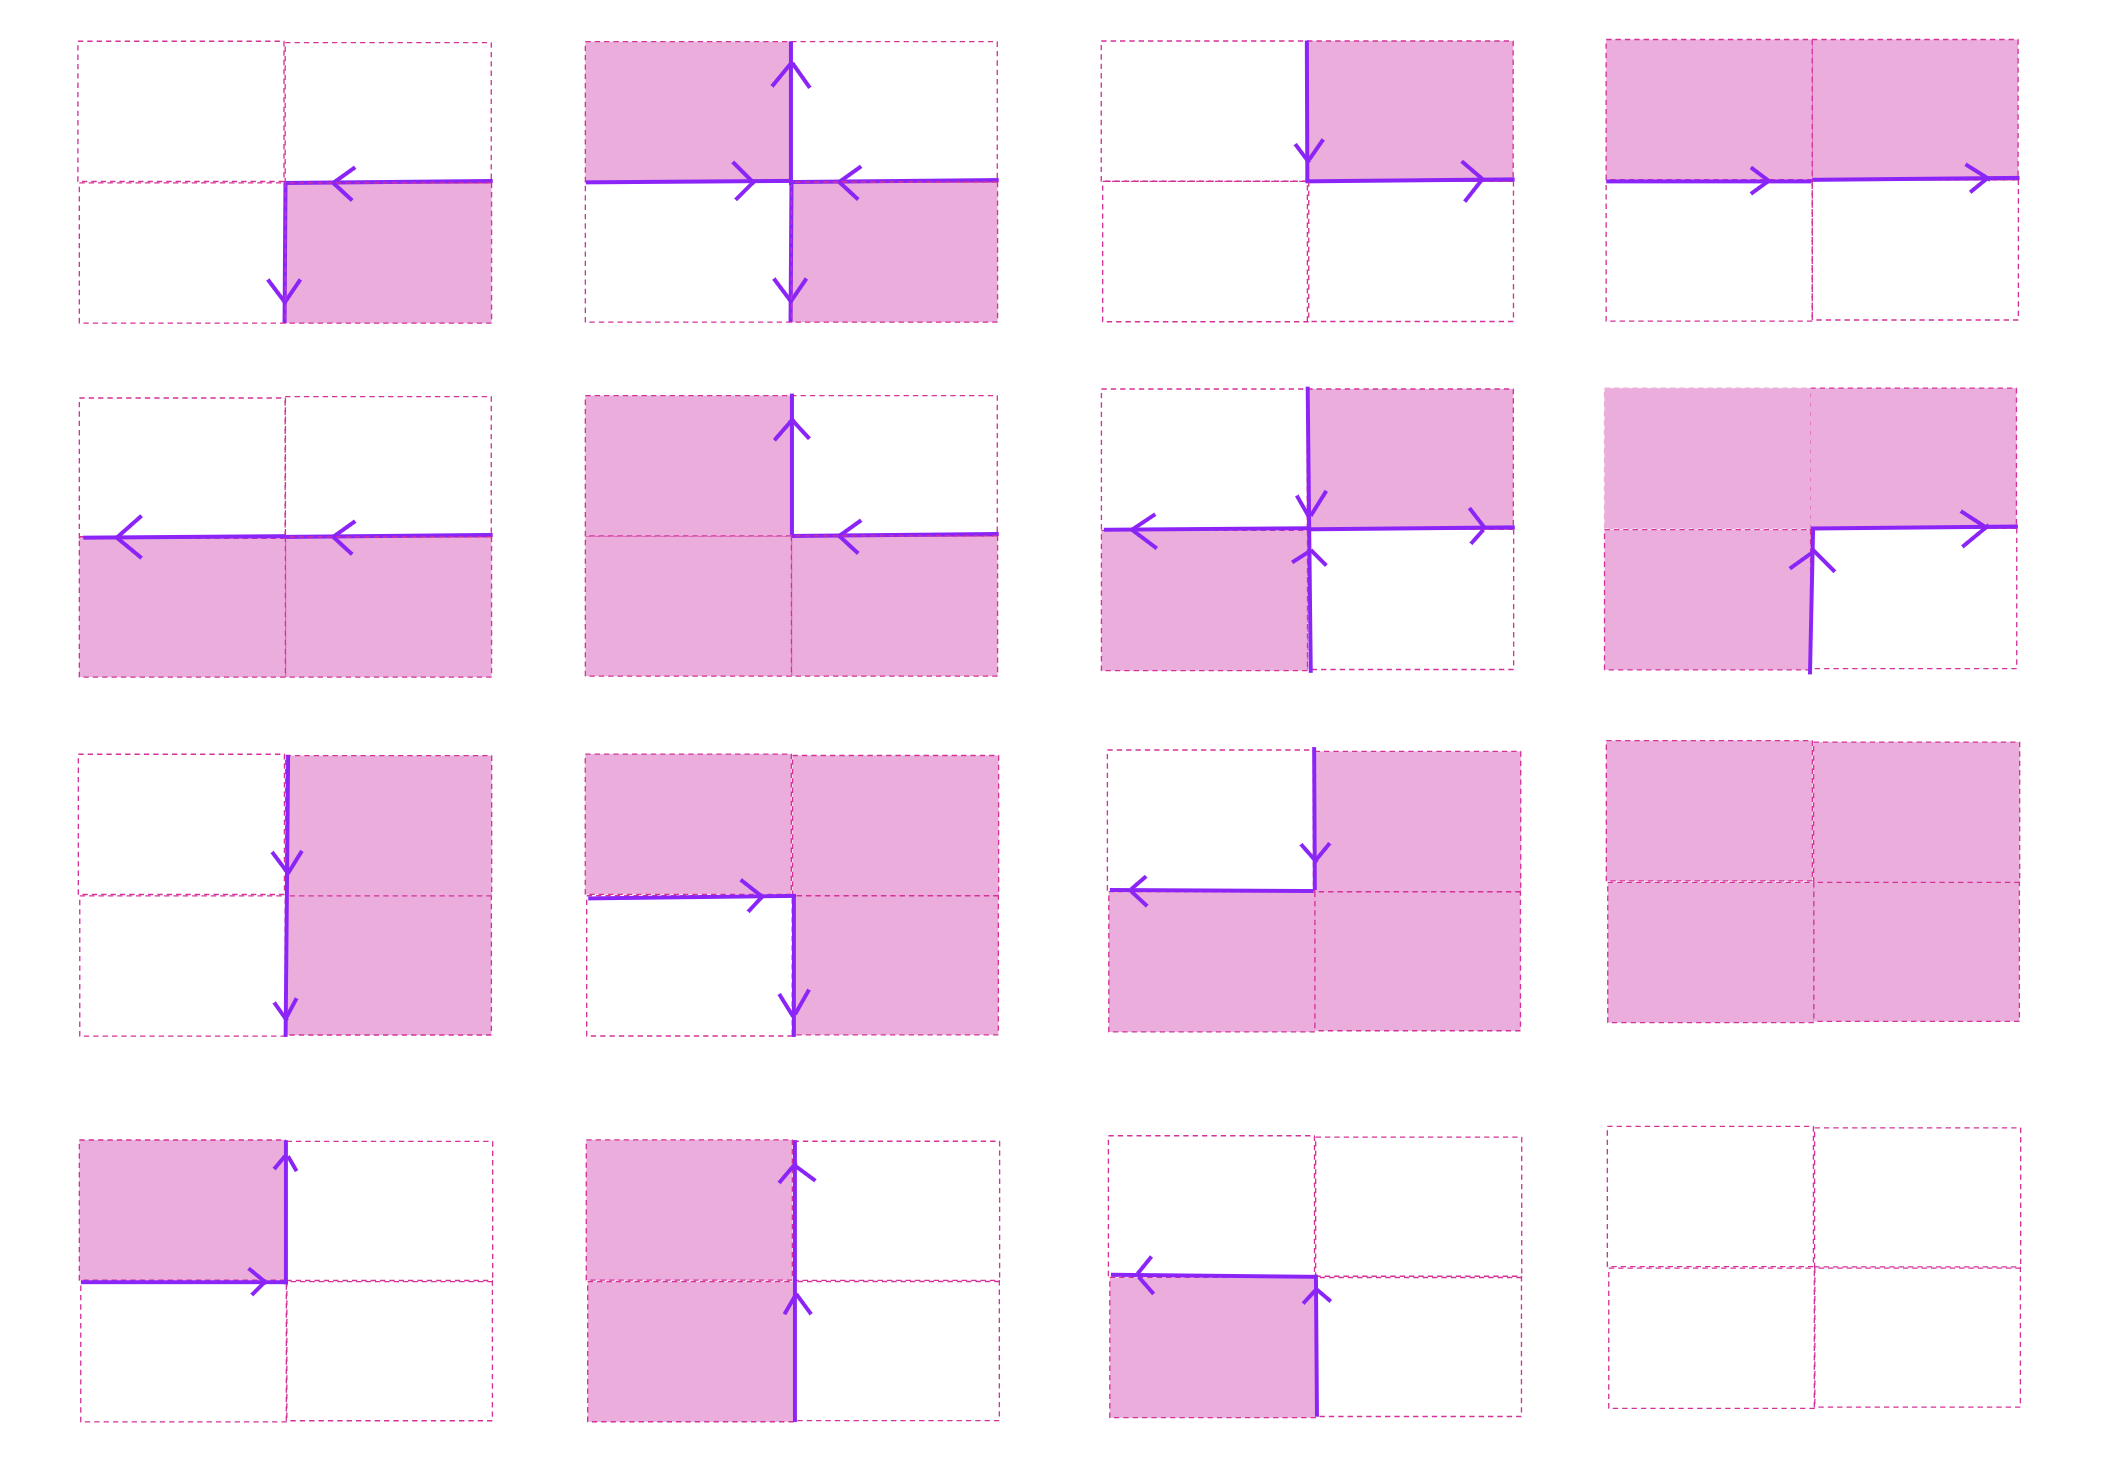
\includegraphics[scale=0.55]{Math_220b_Image_9.png}\newpage\par}

	Based on the prior image, we can assign each edge $\sigma_j$ a successor edge $s(\sigma_j)$ and a\\ predecessor edge $p(\sigma_j)$ such that $p(\sigma_j) + \sigma_j + s(\sigma_j)$ form a connected path. The only times we have any ambiguity on how we can choose $s(\sigma_j)$ and $p(\sigma_j)$ is in the two cases that we have squares diagonal to each other but not sharing any sides. Yet this isn't a big issue since for those two specific cases I can just declare the following convention.

	{\centering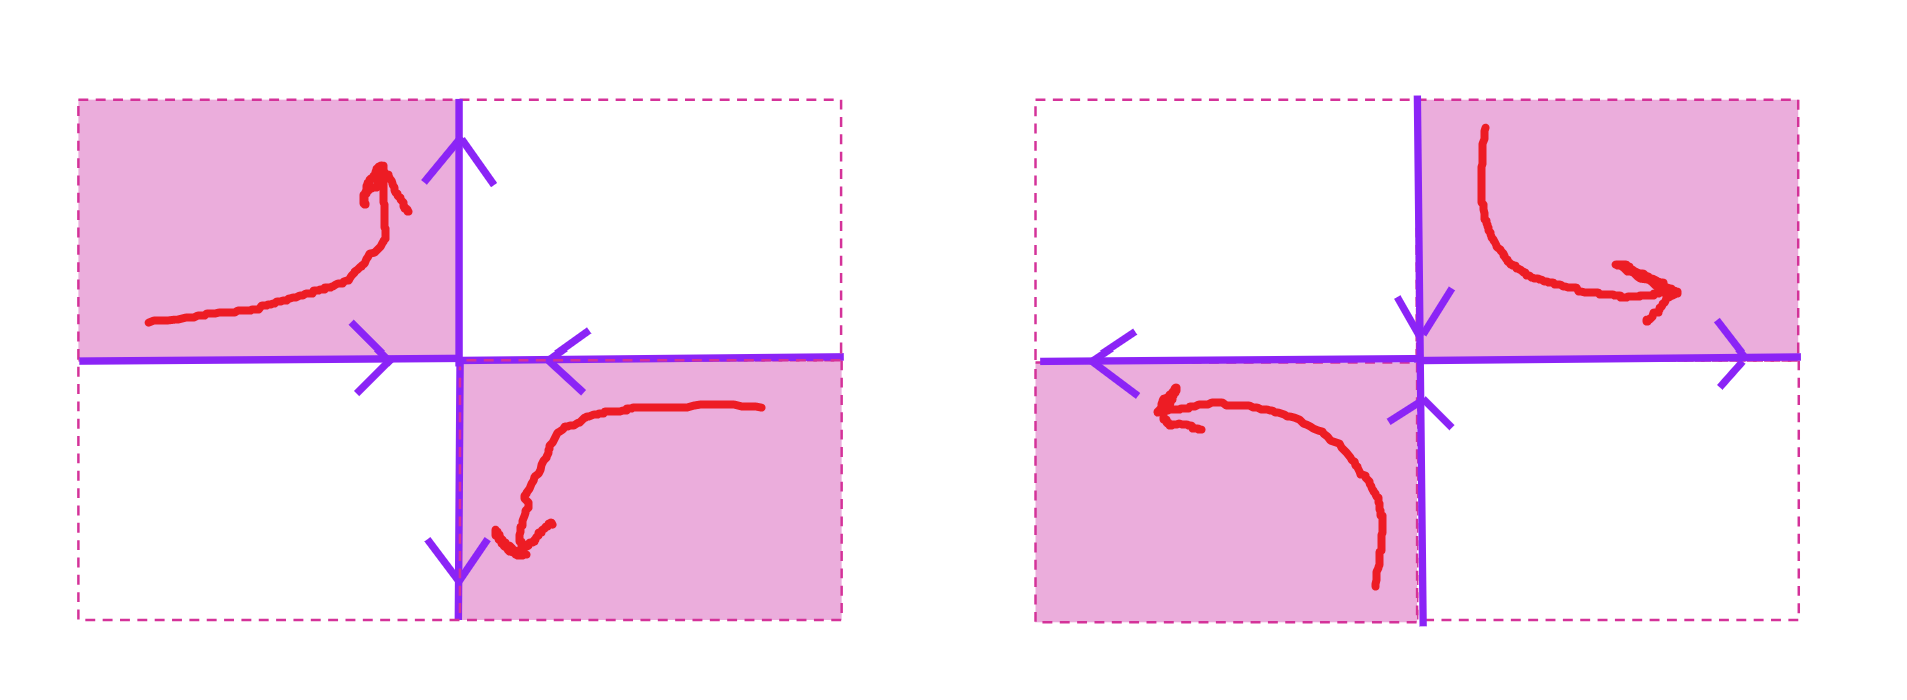
\includegraphics[scale=0.30]{Math_220b_Image_10.png}\retTwo\par}

	With that, we now have that every edge has a unique predecessor and successor edge. Also, we can easily see that $p(s(\sigma_j)) = \sigma_j = s(p(\sigma_j))$. In other words, $s$ and $p$ are inverse functions.\retTwo

	Finally, consider the group action $\mathbb{Z} \curvearrowright \{\sigma_j : 1 \leq j \leq n\}$ given by $k \cdot \sigma_j = s^k(\sigma_j)$. Because there are only finitely many $\sigma_j$, we know every orbit of this group action has only finitely many elements. In particular, given any fixed $\sigma_j$ we claim there exists $N \in \mathbb{N}$ such that $s^{k_1}(\sigma_j) = s^{k_2}(\sigma_j)$ iff $k_2 - k_1 \equiv 0 \mMod{N}$.
	\begin{myIndent}\exPPP
		Why?\\
		Since the orbit of $\sigma_j$ is finite, we know that there exists $0 < k_1^\prime < k_2^\prime$ such that $s^{k_1^\prime}(\sigma_j) = s^{k_2^\prime}(\sigma_j)$. Then by composing on $p^{k_1} = s^{-k_1}$, we get that $\sigma_j = s^{k_2^\prime - k_1^\prime}(\sigma_j)$ where $k_2^\prime - k_1^\prime > 0$. This proves that the set of $k \in \mathbb{N}_{> 0}$ such that $s^k(\sigma_j) = \sigma_j$ is nonempty. So, we can pick a minimal positive $N$ such that $s^N(\sigma_j) = \sigma_j$. It's a basic algebra proof to go from here\dots\retTwo
	\end{myIndent}

	But now the orbit of $\sigma_j$ consists of the collection $\{\sigma_j, s(\sigma_j), \ldots, s^{N-1}(\sigma_j)\}$. This orbit also does not intersect any distinct orbits. Also the concatenated path:
	
	{\center$\sigma_j + s(\sigma_j) + \ldots + s^{N-1}(\sigma_j)$\\ [4pt]\par}
	
	is connected, closed, and does not repeat any distinct edges.\retTwo

	Thus, we define $\pi_1, \ldots, \pi_\ell$ by considering the paths above defined from the orbits of our group action. $\blacksquare$\retTwo
\end{myIndent}

\hTwo\mySepTwo 

The next rabbit hole I want to descend is about $\mathrm{weak}$-$L^p$. After all, this is the one topic from math 240 that even now I've not spent any time trying to learn now that the class is over and my life is somewhat solidified again.\newpage

Let $(X, \mathcalli{M}, \mu)$ be a measure space. Then recall that given any measurable $f: X \to \mathbb{C}$, we define:
\begin{itemize}
	\item the \udefine{distribution function} $\lambda_f: (0, \infty) \to [0, \infty]$ of $f$ to be:
	
	{\centering$\lambda_f(\alpha) \coloneqq \mu(\{x \in X : |f(x)| > \alpha\})$;\retTwo\par}

	\item the \udefine{$\mathrm{weak}$-$L^p$ quasinorm} of $f$ to be:
	
	{\centering $[f]_p \coloneqq \left(\sup\limits_{\alpha > 0} \alpha^p \lambda_f(\alpha)\right)^{1/p} = \sup\limits_{\alpha > 0} \alpha (\lambda_f(\alpha))^{1/p}$ (where $0 < p < \infty$).\retTwo\par}
\end{itemize}

Finally, $\mathrm{weak}$-$L^p$ (also denoted $L^{p,\infty}$) is the collection of all measurable functions $f$ on $X$ such that $[f]_p < \infty$.
\begin{myIndent}\myComment
	Note that by rearranging terms, we can equivalently see that:

	{\centering $[f]_p = \min \{C \in [0, \infty] : \lambda_f(\alpha) \leq \frac{C^p}{\alpha^p} \text{ for all } \alpha > 0\}$ \retTwo\par}

	\begin{myIndent}\pracTwo
		Note that the latter set will in fact always have a minimum. The easiest\\ way to see this is by noting that the latter set's complement (given by\\ $\{C \geq 0 : \lambda_f(\alpha) > \frac{C^p}{\alpha^p} \text{ for some } \alpha > 0\}$) is an open set.
		\retTwo
	\end{myIndent}

	Thus, a function is in $\mathrm{weak}$-$L^p$ precisely iff there is some constant $D > 0$ such that\\ $\mu(\{x : |f(x)| > \alpha\}) \leq \frac{D}{\alpha^p}$ for all $\alpha > 0$.\retTwo
\end{myIndent}

Unsurprisingly we have that $L^p \subseteq \mathrm{weak}$-$L^p$. After all, by Chebishev's inequality we know that $\lambda_f(\alpha) \leq \frac{\|f\|_p^p}{\alpha^p}$ for all $\alpha > 0$. Therefore, it follows that $[f]_p \leq \|f\|_p$. That said, the converse inclusion doesn't generally hold. 
\begin{myIndent}\pracTwo
	For example, consider the sequence $\{\frac{1}{n^{1/p}}\}_{n \in \mathbb{N}}$ as a function in $l^{p}(\mathbb{N})$. Its $l^p$ norm is given by the harmonic series $\sum_{n \in \mathbb{N}} \frac{1}{n}$ which diverges. That said it is in $\mathrm{weak}$-$l^p$. After all:
	
	{\centering$\lambda(\alpha) = \begin{cases} \lfloor \alpha^{-p} \rfloor & \text{ if }\alpha^{-p} \notin \mathbb{N} \\ \alpha^{-p} - 1 & \text{ if } \alpha^{-p} \in \mathbb{N} \end{cases}$\retTwo\par}

	Importantly, this means that $\lambda(\alpha) < \alpha^{-p}$ for all $\alpha > 0$ and we can make their difference arbitrarily small. In turn, we can show that $\sup_{\alpha > 0} \alpha^{p}\lambda(\alpha) = 1$.\retTwo
\end{myIndent}

The big use case of $\mathrm{weak}$-$L^p$ is as follows. Recall that for any $0 < p < \infty$ and measurable function $f$ on $X$ we have that:

{\centering $\int |f|^p \df \mu = p\int_0^\infty \alpha^{p-1}\lambda_f(\alpha) \df \alpha$ \retTwo\par}

But now if $f \in \mathrm{weak}$-$L^p$, we can say that:

{\centering $p\int_0^\infty \alpha^{p-1}\lambda_f(\alpha) \df \alpha \leq p[f]_p^p\int_0^\infty \frac{1}{\alpha} \df \alpha$ \retTwo\par}

In some sense, the latter integral only just barely doesn't converge. So, given slightly more information bounding our function, we can say that $f$ is in $L^p$. To further explore this, here is an exercise from Folland's \textit{Real Analysis}.\newpage

\Hstatement\blab{(Folland) Exercise 6.36:} If $f \in \mathrm{weak}$-$L^p$ and $\mu(\{x : f(x) \neq 0\}) < \infty$, then $f \in L^q$ for\\ all $q < p$.
\begin{myIndent}\HexOne
	Proof:\\
	If $C \coloneqq \mu(\{x : f(x) \neq 0\}) < \infty$, then we know that $\lambda_f(\alpha) \leq C$ for all $\alpha > 0$. In turn,\\ for all $0 < q < p$ we have that:

	{\centering\begin{tabular}{l}
		$\int |f|^q \df \mu = q\int_0^\infty \alpha^{q-1}\lambda_f(\alpha)\df \alpha = q\int_0^1 \alpha^{q-1} \lambda_f(\alpha)\df \alpha + q \int_1^\infty \alpha^{q-1}\lambda_f(\alpha)\df \alpha$\\ [6pt]
		$\phantom{\int |f|^q \df \mu = q\int_0^\infty \alpha^{q-1}\lambda_f(\alpha)\df \alpha} \leq qC\int_0^1 \alpha^{q-1} \df \alpha + q\int_1^\infty \frac{\alpha^{q-1}}{\alpha^p}[f]_p^p \df \alpha$\\ [6pt]
		$\phantom{\int |f|^q \df \mu = q\int_0^\infty \alpha^{q-1}\lambda_f(\alpha)\df \alpha} = C + [f]_p^p \frac{q}{p-q}$.\\ [6pt]
	\end{tabular}\retTwo\par}
\end{myIndent}

On the other hand, if $f \in (\mathrm{weak}$-$L^p) \cap L^\infty$, then $f \in L^q$ for all $q > p$.
\begin{myIndent}\HexOne
	Proof:\\
	If $C \coloneqq \|f\|_\infty < \infty$, then we know that $\lambda_f(\alpha) = 0$ for all $\alpha \geq C$. Hence, we can say for all $p < q < \infty$ that:

	{\centering\begin{tabular}{l}
		$\int |f|^q \df \mu = q\int_0^\infty \alpha^{q-1} \lambda_f(\alpha)\df \alpha = q\int_0^C \alpha^{q-1} \lambda_f(\alpha)\df \alpha$\\ [6pt]
		$\phantom{\int |f|^q \df \mu = q\int_0^\infty \alpha^{q-1} \lambda_f(\alpha)\df \alpha} \leq q\int_0^C [f]_p^p\frac{\alpha^{q-1}}{\alpha^p}\df \alpha = \frac{q}{q - p}C^{q-p}$. $\blacksquare$
	\end{tabular}\retTwo\par}
\end{myIndent}

\hTwo One other thing on this topic I'd like to note is that $[\cdot]_p$ is in fact a \udefine{quasinorm}. After all:
\begin{itemize}
	\item $[f]_p \geq 0$ with $[f]_p = 0$ if and only if $f = 0$ a.e.
	\begin{myIndent}\pracTwo
		$[f]_p \geq 0$ because $\alpha^p \lambda_f(\alpha) \geq 0$ for all $\alpha$. Also, because $\alpha^p > 0$ for all $\alpha > 0$, we have that $\sup_{\alpha > 0}\alpha^p \lambda_f(\alpha) = 0$ if and only if $\lambda_f(\alpha) = 0$ for all $\alpha > 0$. Yet the latter will happen if and only if $\mu(\{x : f(x) \neq 0\}) = 0$.\retTwo
	\end{myIndent}

	\item For any $c \in \mathbb{C}$ we have that $[cf]_p = |c|[f]_p$.
	\begin{myIndent}\pracTwo
		Why?\\
		If $c = 0$ then this is trivial from the last bullet point. Meanwhile, if $c \neq 0$ then:
		
		{\centering$\lambda_{cf}(\alpha) = \mu(\{x : |cf(x)| > \alpha\}) = \mu(\{x : |f(x)| > \frac{\alpha}{|c|}\}) = \lambda_f(\frac{\alpha}{|c|})$\retTwo\par}

		Therefore:

		{\centering $\sup\limits_{\alpha > 0}\alpha^p \lambda_{cf}(\alpha) = \sup\limits_{\alpha > 0} \alpha^p \lambda_{f}(\frac{\alpha}{|c|}) = |c|^p \sup\limits_{\alpha > 0}(\frac{\alpha}{|c|})^p \lambda_f(\frac{\alpha}{|c|}) = |c|^p \sup\limits_{\beta > 0} \beta^p \lambda_f(\beta)$ \retTwo\par}
	\end{myIndent}

	\item \hypertarget{weak L^p has weird triangle inequality}{There} exists $B \geq 1$ such that $[f + g]_p \leq B([f]_p + [g]_p)$ for all measurable functions $f$ and $g$.
	\begin{myIndent}\pracTwo
		Why?\\
		First note that:
		
		{\centering\begin{tabular}{l}
			$\lambda_{f + g}(\alpha) = \mu(\{x : |f(x) + g(x)| > \alpha\}) \leq \mu(\{x : |f(x)| + |g(x)| > \alpha\})$\\ [6pt]
			$\phantom{\lambda_{f + g}(\alpha) = \mu(\{x : |f(x) + g(x)| > \alpha\})} \leq \mu(\{x : |f(x)| > \frac{\alpha}{2}\} \cup \{x : |g(x)| > \frac{\alpha}{2}\})$\\ [6pt]
			$\phantom{\lambda_{f + g}(\alpha) = \mu(\{x : |f(x) + g(x)| > \alpha\})} \leq \mu(\{x : |f(x)| > \frac{\alpha}{2}\}) + \mu(\{x : |g(x)| > \frac{\alpha}{2}\})$\\ [6pt]
			$\phantom{\lambda_{f + g}(\alpha) = \mu(\{x : |f(x) + g(x)| > \alpha\})} = \lambda_f(\frac{\alpha}{2}) + \lambda_g(\frac{\alpha}{2})$
		\end{tabular}\retTwo\par}

		In turn $\sup\limits_{\alpha > 0} \alpha^p \lambda_{f + g}(\alpha) \leq \sup\limits_{\alpha > 0} \alpha^p (\lambda_f(\frac{\alpha}{2}) + \lambda_g(\frac{\alpha}{2})) \leq \sup\limits_{\alpha > 0}\alpha^p \lambda_f(\frac{\alpha}{2}) + \sup\limits_{\beta > 0}\beta^p \lambda_g(\frac{\beta}{2})$.\newpage

		Next note that $\sup\limits_{\alpha > 0}\alpha^p \lambda_f(\frac{\alpha}{2}) = 2^p \sup\limits_{\alpha > 0} (\frac{\alpha}{2})^p \lambda_f(\frac{\alpha}{2}) = 2^p[f]_p^p$.\retTwo Similarly, we have that $\sup\limits_{\beta > 0}\beta^p \lambda_f(\frac{\beta}{2}) = 2^p [g]_p^p$. Thus, we can conclude:

		{\centering $[f + g]_p^p \leq 2^p([f]^p_p + [g]_p^p)$ \retTwo\par}

		In other words, $[f + g]_p \leq 2([f]_p^p + [g]_p^p)^{1/p}$. To finish off, if $p \geq 1$ then this proves that $[f + g]_p \leq 2([f]_p + [g]_p)$.
		\begin{myIndent}\color{VioletRed}
			You can justify to yourself that $(a^p + b^p)^{1/p} \leq a + b$ for all $a, b \geq 0$ when $p \geq 1$ by considering that the $p$-norm on $\mathbb{R}^2$ satisfies the triangle inequality.\retTwo
		\end{myIndent}

		Meanwhile, if $0 < p < 1$, then we need to find a constant $A > 1$ such that\\ $([f]_p^p + [g]_p^p)^{1/p} \leq A([f]_p + [g]_p)$.
	\end{myIndent}
\end{itemize}

\pracOne\mySepTwo
Tangent: While I'm finding this constant $A$, I shall also prove that $L^p$ is a quasinormed space when $0 < p < 1$.\retTwo

\ul{Lemma 1:} If $a, b \geq 0$ and $0 < p < 1$, then $(a + b)^p \leq a^p + b^p$.
\begin{myIndent}\pracTwo
	Proof:\\
	If $a = 0$ then this is obvious. Meanwhile, if $a \neq 0$ then we have that $(a + b)^p \leq a^p + b^p$ if and only if $(1 + \frac{b}{a})^p = (\frac{a + b}{a})^p \leq \frac{a^p + b^p}{a^p} = 1 + (\frac{b}{a})^p$. Therefore, it suffices to show that $(1 + t)^p \leq 1 + t^p$ for all $t \geq 0$.\retTwo

	Set $h(t) = 1 + t^p - (1 + t)^p$. We want to show that $h(t) \geq 0$ for all $t \geq 0$. Fortunately, note that $h(0) = 0$. Also $h^\prime(t) = pt^{p-1} - p(1 + t)^{p-1}$. Since $p - 1 < 0$ and $0 < t < 1 + t$ implies that $(1 + t)^{p-1} < t^{p-1}$, we can conclude that $h^\prime(t) > 0$ for all $t > 0$. This proves that $h$ is strictly increasing for $t > 0$. Hence, we can conclude that $h(t) \geq 0$ for all $t \geq 0$. $\blacksquare$
	\begin{myIndent}\color{VioletRed}
		As a side note, mirror reasoning shows that $h(t)$ is strictly decreasing for $t > 0$\\ if $p > 1$. So, the opposite inequality will hold if $p > 1$.\retTwo
	\end{myIndent}
\end{myIndent}

\ul{Lemma 2:} If $a, b \geq 0$ and $q \geq 1$, then $(a + b)^q \leq 2^{q - 1}(a^q + b^q)$.
\begin{myIndent}\pracTwo
	Proof:\\
	In order to make it clear how someone might have discovered this lemma without seeing the constant $2^{q-1}$ on a google search, I shall specifically write down the process for finding some $A \geq 1$ such that $(a + b)^q \leq A(a^q + b^q)$. Then, it will just so happen to work out that the minimal $A$ that works is $2^{q-1}$.\retTwo
	
	Firstly, note for any $A \geq 1$ that if $a = 0$ then we always have that $(a + b)^q \leq A(a^q + b^q)$. So like before, it suffices to assume $a \neq 0$. Then because $(a + b)^q \leq A(a^q + b^q)$ if and only if $(1 + \frac{b}{a})^q \leq A(1 + (\frac{b}{a})^q)$, it suffices to show that $(1 + t)^q \leq A(1 + t^q)$ for all $t \geq 0$.\retTwo

	Let $h(t) = \frac{A(1 + t^q)}{(1 + t)^q}$. We want to fix $A \geq 1$ such that $h(t) \geq 1$ for all $t \geq 0$. Fortunately, note that $h(0) = A \geq 1$. Also, we can calculate for $t \geq 0$ that:

	{\centering $h^\prime(t) = \frac{Aqt^{q-1}(1 + t)^q - Aq(1 + t^q)(1 + t)^{q-1}}{(1 + t)^{2q}} = \frac{Aq(t^{q-1}(1 + t) - (1 + t^q))}{(1 + t)^{q + 1}} = \frac{Aq(t^{q-1} - 1)}{(1 + t)^{q+1}}$ \newpage\par}

	It follows that $h$ achieves an absolute minimum on $[0, \infty)$ at $t = 1$. So, it suffices to pick $A$ with $h(1) = \frac{2A}{2^q} \geq 1$. The smallest $A$ satisfying this is $A = 2^{q - 1}$. $\blacksquare$\retTwo
\end{myIndent}

As a result of these two lemmas, we can now say for any measurable functions\\ $f, g : X \to \mathbb{C}$ and $0 < p < 1$ that:

{\centering $\|f + g\|_p \leq 2^{\frac{1}{p} - 1}(\|f\|_p + \|g\|_p)$. \retTwo\par}

\begin{myIndent}\pracTwo
	Proof:\\
	As $t \mapsto t^p$ is a strictly increasing function, we can conclude from the triangle inequality that $|f(x) + g(x)|^p \leq (|f(x)| + |g(x)|)^p$ for all $x \in X$. In turn, by applying lemma 1 we get that:

	{\centering\begin{tabular}{l}
		$\int |f(x) + g(x)|^p \df \mu \leq \int (|f(x)| + |g(x)|)^p \df \mu$\\ [6pt]
		$\phantom{\int |f(x) + g(x)|^p \df \mu} \leq \int |f(x)|^p + |g(x)|^p \df \mu = \int |f|^p \df \mu + \int |g|^p \df \mu$
	\end{tabular}\retTwo\par}

	Next, as $\frac{1}{p} > 1$, we can conclude by lemma 2 plus the fact that $t \mapsto t^{1/p}$ is a strictly\\ increasing function that:

	{\centering\begin{tabular}{l}
		$(\int |f(x) + g(x)|^p \df \mu)^{1/p} \leq (\int |f|^p \df \mu + \int |g|^p \df \mu)^{1/p}$\\ [6pt]
		$\phantom{(\int |f(x) + g(x)|^p \df \mu)^{1/p}} \leq 2^{\frac{1}{p} - 1} \left((\int |f|^p \df \mu)^{1/p} + (\int |g|^p \df \mu)^{1/p}\right)$. $\blacksquare$
	\end{tabular}\retTwo\par}
\end{myIndent}

\mySepTwo

\hTwo\begin{itemize}
	\item[\phantom{.}]
	\begin{myIndent}\pracTwo
		Going back to the problem of finding $A$ such that $([f]_p^p + [g]_p^p)^{1/p} \leq A([f]_p + [g]_p)$,\\ [-1pt] note that lemma 2 from the prior tangent tells us that $A = 2^{\frac{1}{p} - 1}$ works. In turn this\\ [2pt] means that $[f + g]_p \leq 2^{1/p}([f]_p + [g]_p)$ if $0 < p < 1$.

		\begin{myIndent}\myComment
			As a side note, in general the $\mathrm{weak}$-$L^p$ quasinorm will not be a true norm (i.e. it won't in general satisfy the triangle inequality). For an example of this, see my notes from math 240b.\retTwo
		\end{myIndent}
	\end{myIndent}
\end{itemize}

Now it's significant that $[\cdot]_p$ is a quasinorm because any vector space $\mathcalli{X}$ equipped with a quasinorm $[\cdot]$ can in turn be equipped with a topology turning that vector space into a topological vector space where convergence is equivalent to  convergence in that quasi-\\norm.
\begin{myIndent}\myComment
	Describing this topology will require another tangent though unfortunately.
	\retTwo
\end{myIndent}

\mySepTwo

\dispDate{3/30/2026}

I'd like to continue the rabbit-hole from yesterday by taking notes on the book \textit{Modern Methods in Topological Vector Spaces} by Albert Wilanksy (see \inLinkRap{Second citation}{citation 2}).\retTwo

To start off, here are some conventions that Wilanksy uses. Given a topological space\\ $(X, \mathcalli{T})$ as well as some $x \in X$, we write $\mathscr{N}_x$ to denote the collection of neighborhoods of $x$. Also, we say a \udefine{local base of neighborhoods of $x$} is a collection $\mathscr{B} \subseteq \mathscr{N}_x$ such that for all $N \in \mathscr{N}_x$ there exists $E \in \mathscr{B}$ with $E \subseteq N$.\newpage
\begin{myIndent}\color{red}\fontsize{12}{14}\selectfont
	Beware: This differs from the definition of a neighborhood base that math 240b and Folland uses in that the sets in $\mathscr{B}$ are \textit{not} required to be open. That said, it is still the case that if $\mathscr{B}$ is a local base of neighborhoods of $x \in X$ then a net $\langle x_i \rangle_{i \in I}$ converges to $x$ if and only if $x_i$ is eventually in each $E \in \mathscr{B}$.\retTwo
\end{myIndent}

While nets have the advantage of looking and acting like sequences, it will also be helpful to introduce a different generalization of the theory of convergence.\retTwo

Given a set $X$ (and denoting its power set as $\mathcal{P}(X)$), we say $\mathscr{F} \subseteq \mathcal{P}(X)$ is a \udefine{filter} if:
\begin{itemize}
	\item $A, B \in \mathscr{F} \Longrightarrow A \cap B \in \mathscr{F}$,
	\item $A \in \mathscr{F}$ and $A \subseteq E \Longrightarrow E \in \mathscr{F}$,
	\item $\emptyset \notin \mathscr{F}$ and $X \in \mathscr{F}$.
\end{itemize}

Also, we say $\mathscr{B} \subseteq \mathcal{P}(X)$ is a \udefine{filterbase} if it is nonempty, doesn't contain $\emptyset$, and is directed by inclusion (i.e if $A, B \in \mathscr{B}$ then there exists $C \in \mathscr{B}$ with $C \subseteq A \cap B$).

\begin{myIndent}\myComment 
	Note that if $\{\mathscr{F}_i\}_{i \in I}$ is a family of filters, then $\bigcap_{i \in I}\mathscr{F}_i$ is also a filter. Therefore, it makes sense to talk about the smallest filter containing some generating collection of sets\\ (assuming any filters containing that collection even exist).\retTwo

	Given a filterbase $\mathscr{B}$, we claim the smallest filter containing $\mathscr{B}$ is the collection:
	
	{\centering$\mathscr{F} \coloneqq \{A \in \mathcal{P}(X) : A \supseteq B \text{ for some } B \in \mathscr{B}\}$.\retTwo\par}

	\begin{myIndent}\pracTwo\fontsize{11}{13}\selectfont
		Why?\\
		It's clear that $\mathscr{F}$ must be contained in any filter containing $\mathscr{B}$. So, it suffices to justify why $\mathscr{F}$ is itself a filter. The only property not obvious from the definition of $\mathcalli{F}$ is that if $A_1, A_2 \in \mathscr{F}$ then so is $A_1 \cap A_2 \in \mathscr{F}$. Fortunately, we can pick $B_1, B_2 \in \mathscr{B}$ with $A_1 \supseteq B_1$ and $A_2 \supseteq B_2$. Next, we can pick $C$ in $\mathscr{B}$ with $C \subseteq B_1 \cap B_2 \subseteq A_1 \cap A_2$. So, $A_1 \cap A_2 \in \mathscr{F}$.\retTwo 
	\end{myIndent}
\end{myIndent}

Given a topological space $(X, \mathcal{T})$ and some $x \in X$, notice that $\mathscr{N}_x$ is a filter. Also a local base of neighborhoods of $x$ is merely a filterbase generating $\mathscr{N}_x$.\retTwo

\pracOne\mySepTwo 
I mentioned before that filters give us an alternate description of convergence to that of nets. Here is what I mean:
\begin{myTindent}\pracTwo
	(note for just this brief aside I'm going back to Folland\dots)\retTwo
\end{myTindent}

Given a topological space $(X, \mathcal{T})$ and a filter $\mathscr{F} \subseteq \mathcal{P}(X)$, we say $\mathscr{F}$ \udefine{converges} to $x$\\ (written as $\mathscr{F} \to x$) iff $\mathscr{N}_x \subseteq \mathscr{F}$. This definition relates to the definition of convergence\\ of nets as follows:
\begin{itemize}
	\item Suppose $\langle x_i\rangle_{i \in I}$ is a net. Then its \udefine{derived filter} is the collection $\mathscr{F}$ of all $E \subseteq \mathcal{P}(X)$ such that $x_i$ is eventually in $E$.
	\begin{myIndent}\pracTwo
		(Hopefully it's obvious why $\mathscr{F}$ is a filter\dots)\retTwo
	\end{myIndent}

	\ul{Lemma:} The net $\langle x_i\rangle_{i \in I}$ converges to $x$ if and only if its derived filter converges to $x$.
	\begin{myIndent}\pracTwo
		This is clear from the fact that $\langle x_i\rangle_{i \in I}$ converges to $x$ iff $x_i$ is eventually in $N$ for all $N \in \mathscr{N}_x$.\newpage
	\end{myIndent}

	\item Given any filter $\mathscr{F}$, we can view $\mathscr{F}$ as a set directed by (reverse) inclusion. Therefore, $\mathscr{F}$ can be used to index a net. We say a net $\langle x_F\rangle_{F \in \mathscr{F}}$ is \udefine{associated} with $\mathscr{F}$ iff $x_F \in F$ for all $F \in \mathscr{F}$.\retTwo
	
	\ul{Lemma:} A filter $\mathscr{F}$ converges to $x$ if and only if all its associated nets converge to $x$.
	\begin{myIndent}\pracTwo
		$(\Longrightarrow)$\\
		Suppose $\langle x_F\rangle_{F \in \mathscr{F}}$ is any net associated with $\mathscr{F}$. To prove that $x_F \to x$, it suffices to show that if $N \in \mathscr{N}_x$ then $x_F$ is eventually in $N$. Fortunately, as $\mathscr{F} \to x$, we know that $N \in \mathscr{F}$. Then for all $F \subseteq N$ we have that $x_F \in N$.\retTwo

		$(\Longleftarrow)$\\
		If $\mathscr{F} \not\to x$ then there must exist some neighborhood $N$ of $x$ such that $N \notin \mathscr{F}$. In turn, given any $F \in \mathscr{F}$ we must have that $F - N \neq \emptyset$. After all we'd have a contradiction if $F \subseteq N$.\retTwo

		For each $F \in \mathscr{F}$ pick $x \in F$ with $x \notin N$. Then $\langle x_F\rangle_{F \in \mathscr{F}}$ is a net associated with $\mathscr{F}$ but it does not converge to $x$ since $x_F$ is not eventually in $N$. $\blacksquare$\retTwo
	\end{myIndent}
\end{itemize}
\mySepTwo

\hTwo One more definition is as follows. If $V$ is a vector space, we say a collection $\mathscr{B} \subseteq \mathcal{P}(V)$ is \udefine{additive} if for each $B \in \mathscr{B}$ there exists $A \in \mathscr{B}$ with $A + A \subseteq B$.\retTwo

\exTwo\ul{Theorem 4-3-5:} Let $\mathcalli{X}$ be a real or complex vector space. Let $\mathscr{B}$ be an additive filterbase\\ of balanced absorbing subsets of $\mathcalli{X}$. Then there is a unique topology turning $\mathcalli{X}$ into a\\ topological vector space and satisfying that $\mathscr{B}$ is a local base of neighborhoods of $0$.
\begin{myIndent}\exThreeP
	\begin{myIndent}\color{RawerSienna}
		(See \inLinkRap{placeholder}{pages 230-232} for a refresher on the definitions of a balanced set and an\\ absorbing set in a real or complex vector space. Importantly, even though I've priorly only used those terms when referring to vector spaces already equipped with some topology, the definitions of those terms are purely algebraic. So it still makes sense to talk about balanced sets and absorbing sets in any real or complex vector space.)\retTwo
	\end{myIndent}

	Proof (Existence):\\
	We define our topology how one would reasonably expect. We shall say $U \subseteq \mathcalli{X}$ is open if and only if for all $x \in U$ there exists $B \in \mathscr{B}$ with $x + B \subseteq U$.\retTwo

	\ul{Claim 1:} This defines a topology on $\mathcalli{X}$.
	\begin{itemize}\exPPP
		\item It's trivial that $\emptyset$ and $\mathcalli{X}$ are both open.
		
		\item Suppose $U_1$, $U_2$ are both open. Then for any $x \in U_1 \cap U_2$, we can pick $B_1, B_2 \in \mathscr{B}$ with $x + B_1 \subseteq U_1$ and $x + B_2 \subseteq U_2$. Since $\mathscr{B}$ is a filterbase, we know there exists $B \in \mathscr{B}$ with $B \subseteq B_1 \cap B_2$. In turn, $x + B \subseteq (x + B_1) \cap (x + B_2) \subseteq U_1 \cap U_2$. As $x$ was arbitrary, this proves that $U_1 \cap U_2$ is open.\retTwo
		
		By induction we can conclude that finite intersections of open sets are open.\newpage

		\item Suppose $\{U_\alpha\}_{\alpha \in A}$ is a family of open sets. Then if $x \in U \coloneqq \bigcup_{\alpha \in A} U_\alpha$, we know that $x \in U_{\alpha_0}$ for some $\alpha_0$. So, there exists $B \in \mathscr{B}$ with $x + B \subseteq U_{\alpha_0} \subseteq U$. Since $x$ was arbitrary, this proves that $\bigcup_{\alpha \in A} U_\alpha$ is open.\retTwo
	\end{itemize}

	\ul{Claim 2:} $\mathscr{B}$ is a local base of neighborhoods of $0$. 
	\begin{myIndent}\exPPP
		To start off, if $N$ is a neighborhood of $0$, then there exists an open set $U$ such that $0 \in U \subseteq N$. In turn, by how we defined our topology we know there exists $B \in \mathscr{B}$ with $B = 0 + B \subseteq N$. This shows that $\mathscr{N}_0$ is contained in the filter generated by $\mathscr{B}$.\retTwo

		To finish showing that $\mathscr{N}_0$ is the filter generated by $\mathscr{B}$, we need to show that $\mathscr{B} \subseteq \mathscr{N}_0$ (i.e. all $B \in \mathscr{B}$ are neighborhoods of $0$ in $\mathcalli{X}$). So consider any $B \in \mathscr{B}$ and define $U \coloneqq \{x \in \mathcalli{X} : x + A \subseteq B \text{ for some } A \in \mathscr{B}\}$.
		\begin{itemize}
			\item Note that as each $A \in \mathscr{B}$ contains $0$ (since each $A$ is balanced), we know that $U \subseteq B$.
			\item Also $0 \in U$ as $0 + B = B$.
			\item Finally, consider any $x \in U$. Then by the definition of $U$ there exists $A \in \mathscr{B}$\\ with $x + A \subseteq B$. And since $\mathscr{B}$ is additive, we can find a set $C \in \mathscr{B}$ with\\ $C + C \subseteq A$. We claim that $x + C \subseteq U$. After all, suppose $y \in x + C$.\\ Then $y + C \subseteq x + C + C \subseteq x + A \subseteq B$. This proves that $y \in U$, and\\ since $y$ was arbitrary, we conclude that $x + C \subseteq U$. Finally, by the definition\\ of an open set plus the arbitrariness of $x$, this proves that $U$ is open.\retTwo
		\end{itemize}
	\end{myIndent}

	As an important side note, by slightly modifying the proof of the prior claim we can also show $x + B$ is a neighborhood of $x$ for all $B \in \mathscr{B}$. Yet also since for any open set $U$ containing $x$ we have that there exists some $B \in \mathscr{B}$ with $x + B \subseteq U$, we can thus conclude that $x + \mathscr{B} \coloneqq \{x + B : B \in \mathscr{B}\}$ is a local base of neighborhoods of $x$ for any $x \in \mathcalli{X}$. This will be used in the proof of the third and final claim.\retTwo

	\ul{Claim 3:} The vector space operations are continuous with respect to our defined topology.
	\begin{myIndent}\exPPP
		First we show vector addition is continuous. Consider any $x, y \in \mathcalli{X}$ and let $N$ be any neighborhood of $x + y$. Then it suffices to show that there are neighborhoods $N_x$ and $N_y$ of $x$ and $y$ respectively such that $x^\prime + y^\prime \in N$ for any $x^\prime \in N_x$ and $y^\prime \in N_y$. Fortunately, we know there exists $B \in \mathscr{B}$ with $x + y + B \subseteq N$. Next as $\mathscr{B}$ is additive, we know there exists $A \in \mathscr{B}$ with $A + A \subseteq B$. So, set $N_x = x + A$ and $N_y = y + A$. Then $N_x + N_y = x + y + A + A \subseteq x + y + B \subseteq N$.\retTwo

		Next, we show scalar multiplication is continuous. Consider any $c \in \mathbb{C}$ (or $\mathbb{R}$) and $x \in \mathcalli{X}$. Then again let $N$ be any neighborhood of $cx$. Then it suffices to find a neighborhood $N_x$ of $x$ in $\mathcalli{X}$ and a disk $\Delta_c$ about $c$ in $\mathbb{C}$ (or $\mathbb{R}$) such that $c^\prime x^\prime \in N$ for all $c^\prime \in \Delta_c$ and $x^\prime \in N_x$.\retTwo

		Let $B \in \mathscr{B}$ satisfy that $cx + B \subseteq N$. Then by the additivity of $\mathscr{B}$ we can pick $A \in \mathscr{B}$ such that $A + A + A + A \subseteq B$. Also, we can pick $D \in \mathscr{B}$ with $D \subseteq A$ and $cD \subseteq A$.
		\begin{myIndent}\color{orange}
			To see why, let $n \in \mathbb{N}_{> 0}$ satisfy that $2^n \geq |c|$. Then choose $D$ such that $\underbracket{D + \ldots + D}_{2^n \text{ terms }} \subseteq A$. Since $D$ is balanced, we have that:
			
			{\centering$cD \subseteq 2^nD  \subseteq \underbracket{D + \ldots + D}_{2^n \text{ terms }} \subseteq A$\newpage\par}
		\end{myIndent}

		Since $D$ is absorbing and contains $0$, we can find some $r > 0$ such that $\alpha x \in D$ when $|\alpha| \leq r$. Let $\Delta_c$ be the disk of radius $r$ centered at $c \in \mathbb{C}$ (or $\mathbb{R}$). Also let $N_x = x + D$. Then we claim that $\Delta_c N_x \subseteq N$.

		\begin{myIndent}\color{orange}
			Suppose $y \in N_x = x + D$ and $c^\prime = c + \alpha \in \Delta_c $ where $|\alpha| < r$. Then:

			{\centering $c^\prime y = (c + \alpha)(y-x + x) = c(y-x) + cx + \alpha(y-x) + \alpha x$ \retTwo\par}

			But $y - x \in D$. Therefore, we can conclude that $c(y - x) \in cD \subseteq A$. Also as $|\alpha| < r$, we have that $\alpha x \in D \subseteq A$.\retTwo

			Finally, without loss of generality we can assume $r < 1$. Then as $D$ is balanced and $|\alpha| < r$, we have that $\alpha(y - x) \in \alpha D \subseteq D \subseteq A$. So, we can conclude that $c^\prime y \in cx + A + A + A \subseteq cx + B \subseteq N$.\retTwo
		\end{myIndent}
	\end{myIndent}

	\mySepThree

	Proof (Uniqueness):\\
	To see that the topology we just defined is unique, first note that any topology satisfying\\ our theorem must have the same collection $\mathscr{N}_0$ of neighborhoods of $0$. In other words,\\ $\mathscr{B}$ uniquely determines the neighborhoods of $0$. Secondly, note that if our topology is\\ specifically a vector space topology, then the convergence of any net is uniquely determined based on the neighborhoods of $0$. Therefore, every topology satisfying our theorem will have the same nets converging. This proves that every topology satisfying our theorem is equal (see \inLinkRap{placeholder}{page 229}). $\blacksquare$\retTwo
\end{myIndent}

\hTwo As a special case of the prior theorem, we can prove that every quasinormed vector space (with quasinorm $[\cdot]$) has a unique vector space topology such that $\langle x_i \rangle_{i \in I}$ converges to $x$ if and only if $[x_i - x] \to 0$.
\begin{myIndent}\exThreeP
	Proof:\\
	Let $\mathscr{B} \coloneqq \{B_r = \{x \in \mathcalli{X} : [x] < r\} : r > 0\}$. Checking that $\mathscr{B}$ is a filterbase consisting of balanced absorbing sets is trivial. The only nonobvious statement is that $\mathscr{B}$ is additive. Consider any $r > 0$ and pick $C \geq 1$ satisfying that $[x + y] \leq C([x] + [y])$ for all $x, y \in \mathcalli{X}$. Then given any $\ell < \frac{r}{2C}$ we have for all $x, y \in B_\ell$ that $[x + y] \leq C([x] + [y]) \leq 2C\ell < r$. Therefore $B_\ell + B_\ell \subseteq B_r$.\retTwo

	By the prior theorem, there is thus a unique vector space topology with $\mathscr{B}$ as a local base of neighborhoods of $0$. Finally, note that a net $\langle x_i\rangle_{i \in I}$ in this topology converges to $0$ iff $x_i$ is eventually in $B_r$ for every $B_r \in \mathscr{B}$, and in turn that happens iff $[x_i] \to 0$. By applying a translation, we can thus see that the topology we constructed here is the topology of convergence with respect to this quasinorm.\retTwo

	\begin{myIndent}\myComment
		As a side note, one particularly cursed observation we can make is that we shouldn't generally expect the balls $B_r \coloneqq \{x : [x] < r\}$ to be open (even though they are\\ neighborhoods of $0$).\retTwo
		
		After all suppose $[x] < r$ and $[z + x] \leq C([z] + [x])$ for all $z \in \mathcalli{X}$. Then if $B_r$ were open we must be able to find a ball $B_\ell(x) \coloneqq \{y : [y - x] < \ell\}$ such that $B_\ell(x) \subseteq B_r$. In other words, given that $[y - x] < \ell$ we'd want to know that\newpage $[y] \leq C([y - x] + [x]) < r$. Yet assuming $C > 1$, we can pick $x$ with $C[x] > r$. Therefore we'd need to have that $C \ell < r - C[x] < 0$. Yet as $C$ and $\ell$ are positive, this is impossible.
		\begin{myIndent}\color{orange}
			On an optimistic note, you can interpret the prior reasoning as proving that $B_{r/C}$ is contained in the interior of $B_r$.\retTwo
		\end{myIndent}

		If we can get a sharper estimate for $[x + y]$ though, then it may be the case that all the balls are open. For example, the quasinorm topology on $\mathrm{weak}$-$L^p$ does contain all the balls $\{f \in \mathrm{weak}$-$L^p : [f - g]_p < r\}$ (where $g \in \mathrm{weak}$-$L^p$ and $r > 0$).\retTwo
	\end{myIndent}
\end{myIndent}

\Hstatement\mySepTwo

\ul{Claim:} Suppose $g \in B_r \coloneqq \{f \in \mathrm{weak}$-$L^p : [f]_p < r\}$. Then there exists a ball\\ $B_\ell(g) \coloneqq \{f \in \mathrm{weak}$-$L^p : [f - g] < \ell\}$ which is contained in $B_r$. Hence, $B_r$ is open.
\begin{myIndent}\HexOne
	Proof:\\
	Given any $t \in (0, 1)$, we can conclude that $\lambda_{f}(\alpha) \leq \lambda_{f - g}((1 - t)\alpha) + \lambda_g(t\alpha)$. Then in turn, like on \inLinkRap{weak L^p has weird triangle inequality}{pages 794-795} we have that:
	
	{\centering$[f]_p \leq \left(\frac{1}{(1 - t)^p}[f - g]_p^p + \frac{1}{t^p}[g]_p^p\right)^{1/p}$\retTwo\par}

	Now we want to find some $\ell$ such that if $[f - g]_p < \ell$ then $[f]_p < r$. Fortunately, for all $t \in (0, 1)$ we have that:
	
	{\centering$\left(\frac{1}{(1 - t)^p}[f - g]_p^p + \frac{1}{t^p}[g]_p^p\right)^{1/p} < r$ if and only if $[f - g]_p^p < (1 - t)^p (r^p - \frac{1}{t^p}[g]_p^p)$\retTwo\par}

	As $[g]_p < r$, we can fix $t$ close enough to $1$ such that $r^p - \frac{1}{t^p}[g]_p^p$ is positive. Then as $(1 - t)^p$ is also positive, we can conclude that $(1 - t)^p (r^p - \frac{1}{t^p}[g]_p^p) > 0$. So, there exists some $\ell > 0$ such that if $\ell^p < (1 - t)^p (r^p - \frac{1}{t^p}[g]_p^p)$. Then $[f - g]_p < \ell$ implies that $[f]_p < r$. $\blacksquare$\retTwo
\end{myIndent}

\ul{Corollary:} The quasinorm topology on $\mathrm{weak}$-$L^p$ is the topology generated (in the typical\\ topological sense) by the balls $B_\ell(g) \coloneqq \{f \in \mathrm{weak}$-$L^p : [f - g] < r\}$ (where $g \in \mathrm{weak}$-$L^p$\\ and $r > 0$).\retTwo

\hTwo\mySepTwo 

\dispDate{3/31/2026}

\blect{Math 220C Lecture Notes:}\retTwo

A convention I will be using during spring quarter is that if $\Omega \subseteq \mathbb{R}^m$ is an open set and $u: \Omega \to \mathbb{R}$ is a function, then I may denote the $j$th partial derivative of $u$ as $u_{x_j}$. Also $u_{x_j, x_k}$ will refer to $(u_{x_j})_{x_k}$ as opposed to $(u_{x_k})_{x_j}$. Usually this distinction won't matter though since we'll typically assume we are working with functions that are $C^2$ if we need second order partial derivatives.\retTwo

In specifically math 220c, we'll often identify $\mathbb{C}$ with $\mathbb{R}^2$ via the isometry $x + iy \mapsto (x, y)$. Thus if $f$ is a complex variable function, we shall refer to $\partial_x f = f_x$ as the resulting partial derivative in the direction of the real axis. And similarly, $\partial_y f = f_y$ will be the partial derivative of $f$ in the direction of the imaginary axis.\newpage

Recall from \inLinkRap{placeholder}{page 332} that if $G \subseteq \mathbb{C}$ is a region, we say $u: G \to \mathbb{R}$ is a \udefine{harmonic} function if $u \in C^2(G)$ and $u_{x,x} + u_{y,y} = 0$.
\begin{myIndent}\pracTwo
	For example, if $f \in O(G)$ then $u = \rea{f}$ and $v = \ima{f} = \rea{-i f}$ are both harmonic functions. In this case, we say $u$ and $v$ are \udefine{harmonic conjugates}.\retTwo
\end{myIndent}

\exTwo\ul{Lemma:} If $G$ is simply connected, then any harmonic function $u: G \to \mathbb{R}$ admits a\\ harmonic conjugate.
\begin{myIndent}\exThreeP
	Proof:\\
	Let $F = u_x - iu_y$ be a function from $G$ to $\mathbb{C}$. Then note that $F \in C^1(G)$ and satisfies the Cauchy-Riemann equations. After all $(u_{x})_x = (-u_y)_y$ by the \udefine{Laplace equation} (i.e. the PDE defining harmonic functions). Meanwhile $(u_x)_y = -(-u_y)_x$ is true since $u \in C^2(G)$. It follows that $F$ is a holomorphic function. And since $G$ is simply connected, we in turn know that $F = f^\prime$ for some $f \in O(G)$.\retTwo

	Write $f(x + iy) = \alpha(x + iy) + i\beta(x + iy)$ where $\alpha, \beta$ are real-valued functions. Since $f^\prime$ exists (and equals $F$), we can get $f^\prime$ by differentiating in whatever direction we find convenient. In other words, we know that $u_x - iu_y = F = f^\prime = \alpha_x + i\beta_x$. In turn, we know that $u_x = \alpha_x$ and $-u_y = \beta_x$. Since $f$ is holomorphic and thus satisfies the Cauchy-Riemann equations, we also know $\beta_x = -\alpha_y$. So, this proves that $u_y = \alpha_y$.\retTwo

	Since $u$ and $\alpha$ have the same partial derivatives, we can thus conclude that $u = \alpha + C$ where $C$ is some constant. Yet without loss of generality we can assume $C = 0$. After all, if not then $f - C$ is as valid a primitive of $F$ as $f$. Finally, we now have that a harmonic conjugate of $u$ is given by the function $\beta$. $\blacksquare$\retTwo
\end{myIndent}

\hTwo We can also prove the converse statement (as is shown by the following homework\\ exercises). The key observation to make is just that even if an open set $U \subseteq \mathbb{C}$ isn't\\ simply connected, every point in $U$ still has a simply connected neighborhood contained in $U$ (namely some disk of small enough radius). Therefore, any harmonic function \textit{locally} admits a harmonic conjugate. And since satisfying a PDE is a local property, that is often enough for our purposes.\retTwo

\Hstatement\mySepTwo 

\blab{Set 1 Problem 1:} \hypertarget{Math 220c Set 1 Problem 1}{If} $U, V$ are connected open sets in $\mathbb{C}$, $g: V \to U$ is holomorphic, and\\ $u: U \to \mathbb{R}$ is harmonic, then $u \circ g: V \to \mathbb{R}$ is harmonic in $V$.
\begin{myIndent}\HexOne
	Proof:\\
	Given any $z \in V$, by the continuity of $g$ we can find disks $\Delta_z \subseteq V$ and $\Delta_{g(z)} \subseteq U$ centered at $z$ and $g(z)$ respectively such that $g(\Delta_{z}) \subseteq \Delta_{g(z)}$. Then as $\Delta_{g(z)}$ is simply connected, we know $u$ has a harmonic conjugate on $\Delta_{g(z)}$. So, we can consider a holomorphic function $f: \Delta_{g(z)} \to \mathbb{C}$ satisfying that $\rea{f} = u$.\retTwo

	To finish off, by chain rule we know that $f \circ g$ is a holomorphic function on $\Delta_z$. Also, we have that $\rea{f \circ g} = u \circ g$. This proves that $u \circ g$ is a harmonic function on $\Delta_z$. Since $z$ was arbitrary, this proves that $(u \circ g)_{x,x} + (u \circ g)_{y,y} = 0$ everywhere on $U$. So, $u \circ g$ is harmonic in $V$. $\blacksquare$\retTwo
\end{myIndent}

\blab{Set 1 Problem 3:} \hypertarget{Math 220c Set 1 Problem 3}{Let} $G \subseteq \mathbb{C}$ be open and connected.\newpage
\begin{enumerate}
	\item[(i)] Show that if $h : G \to \mathbb{C}$ is holomorphic and nowhere zero in $G$, then $u(z) = \log |h(z)|$ is harmonic in $G$.
	\begin{myIndent}\HexOne
		Let $u(z) \coloneqq \log|z|$. If we can show that $u$ is harmonic in $\mathbb{C} - \{0\}$, then the statement we are trying to prove is just an application of problem 1.\retTwo

		Fortunately, note that $u(x + iy) = \log(\sqrt{x^2 + y^2}) = \frac{1}{2}\log(x^2 + y^2)$. Therefore, we can calculate that $u_x(x + iy) = \frac{x}{x^2 + y^2}$ and in turn:
		
		{\centering$u_{x,x}(x + iy) = \frac{x^2 + y^2 - x(2x)}{(x^2 + y^2)^2} = \frac{y^2 - x^2}{(x^2 + y^2)^2}$.\retTwo\par}
		
		By symmetry, we thus also have that $u_{y,y}(x + iy) = \frac{x^2 - y^2}{(x^2 + y^2)^2}$. Hence, $u_{x,x} + u_{y,y} = 0$.\retTwo

		Also $u \in C^\infty(\mathbb{C} - \{0\})$ as $t \mapsto \log(t)$ is a smooth function from $(0, \infty)$ to $\mathbb{R}$ and $(x, y) \mapsto \sqrt{x^2 + y^2}$ is a smooth function from $\mathbb{R}^2 - \{(0, 0)\}$ to $(0, \infty)$. This finishes the proof that $u$ is harmonic in $\mathbb{C} - \{0\}$.
	\end{myIndent}
	
	\item[(ii)] Show that $G$ is simply connected if every harmonic function in $G$ admits a harmonic\\ conjugate.
	\begin{myIndent}\HexOne
		Let $h \in O(G)$ be any nowhere zero holomorphic function on $G$. To prove that $G$ is simply connected, it suffices to proves that $G$ is a logarithm domain, and to do that it suffices to prove that there exists a function $g \in O(G)$ with $h(z) = e^{g(z)}$.\retTwo

		Yet since every harmonic function in $G$ admits a harmonic conjugate and we know from part (i) that $\log |h(z)|$ is harmonic in $G$, we know that there is a holomorphic function $g \in O(G)$ with $\rea{g(z)} = \log|h(z)|$. Next, we consider the function $f(z) \coloneqq \frac{h(z)}{e^{g(z)}}$. Importantly, $f \in O(G)$ and $|f(z)| = \frac{|h(z)|}{e^{\rea{g(z)}}} = \frac{|h(z)|}{e^{\log|h(z)|}} = 1$ for all $z \in G$. By the maximum modulus principle, we can thus conclude that $f$ is a constant function (with magnitude $1$). And this proves that there exists some $C \in \mathbb{C}$ with $|C| = 1$ and $Ce^{g(z)} = h(z)$. Finally, write $C = e^{is}$ for some $s \in [-\pi, \pi)$. Then $h(z) = e^{g(z) + is}$. This proves that $h$ has a logarithm.\retTwo
	\end{myIndent}
	
	\item[(iii)] Show that $u(z) = \log|z|$ admits no harmonic conjugate in $G = \mathbb{C} - \{0\}$.
	\begin{myIndent}\HexOne
		Suppose for the sake of contradiction that $u$ has a harmonic conjugate\\ $v: \mathbb{C} - \{0\} \to \mathbb{R}$. Then, we'd know the function $f(z) \coloneqq u(z) + iv(z)$ is\\ a holomorphic function in $O(\mathbb{C} - \{0\})$ satisfying that $|e^{f(z)}| = e^{u(z)} = |z|$\\ for all $z \in \mathbb{C} - \{0\}$. Thus by identical reasoning to that of part (ii), we can\\ conclude that there exists some $C \in \mathbb{C}$ with $|C| = 1$ and $Ce^{f(z)} = z$ on\\ $\mathbb{C} - \{0\}$. In turn, this would imply the existence of a branch of the logarithm\\ function on $G = \mathbb{C} - \{0\}$.\retTwo

		Yet we know no branch of the logarithm exists on $G$. 
		\begin{myIndent}\HexTwoP
			If such a branch did exist, then we'd have to have that $\frac{1}{z}$ has a primitive on\\ $\mathbb{C} - \{0\}$. In turn, we'd have to have that $\int_{|z| = 1} \frac{1}{z}\df z = 0$. Yet we can\\ calculate that $\int_{|z| = 1} \frac{1}{z}\df z = \pm 2\pi i \neq 0$. \HexOne $\blacksquare$\retTwo
		\end{myIndent}
	\end{myIndent}
\end{enumerate}

\mySepTwo\newpage

\exTwo\ul{Corollary (Elliptic Regularity):} \hypertarget{Page 804 Elliptic Regularity}{If} $U \subseteq \mathbb{C}$ is open and $u: U \to \mathbb{R}$ is a harmonic function then $u$ is smooth.
\begin{myIndent}\exThreeP
	Proof:\\
	Given any $x \in U$ we can consider a disk $\Delta_x \subseteq U$ centered at $x$. Then $u|_{\Delta_x} = \rea{f}$ for\\ [-2pt] some $f \in O(\Delta_x) \subseteq C^\infty(\Delta_x)$. Since $f$ is smooth, we thus know that $u = \rea{f} = \frac{f + \overline{f}}{2}$ is also smooth on $\Delta_x$ (and in particular at $x$). $\blacksquare$\retTwo
\end{myIndent}

\hTwo Given a continuous function $u: G \to \mathbb{R}$, we say $u$ has the \udefine{mean value property} if for all $a \in G$ and $r > 0$ such that $\overline{\Delta}(a, r) \subseteq G$ we have that $u(a) = \frac{1}{2\pi}\int_0^{2\pi} u(a + re^{it})\df t$.\retTwo

\exTwo\ul{Theorem:} \hypertarget{harmonic functions have MVP}{If} $u: G \to \mathbb{R}$ is harmonic then $u$ satisfies the mean value property.
\begin{myIndent}\exThreeP
	Proof:\\
	Suppose $\overline{\Delta}(a, r) \subseteq G$. Then there exists $R > r$ such that $\Delta(a, R) \subseteq G$. And since $\Delta(a, R)$ is simply connected, there exists a holomorphic function $f \in O(a, R)$ such that $u = \rea{f}$.\retTwo

	By Cauchy's formula, we have that:
	
	{\centering$f(a) = \frac{1}{2\pi i}\int_{|z - a| = r}\frac{f(z)}{z - a}\df z = \frac{1}{2\pi i}\int_0^{2\pi} \frac{f(a + re^{it})}{re^{it}}ire^{it}\df t = \frac{1}{2\pi}\int_0^{2\pi} f(a + re^{it})\df t$.\retTwo\par}

	Then by taking the real parts of both sides, we get that $u(a) = \frac{1}{2\pi}\int_0^{2\pi}u(a + re^{it})\df t$. $\blacksquare$\retTwo
\end{myIndent}

\exTwo\ul{Theorem:} \hypertarget{220c Maximal Principle for harmonic functions}{Let} $G \subseteq \mathbb{C}$ be open and connected. If $u: G \to \mathbb{R}$ is continuous and satisfies the mean value property, then $u$ satisfies the \udefine{maximal principle}, meaning that if there exists $a \in G$ with $u(a) \geq u(z)$ for all $z \in G$ then $u$ is a constant function.
\begin{myIndent}\exThreeP
	Proof:\\
	Suppose such an $a$ exists and set $\Omega \coloneqq \{z \in G : u(z) = u(a)\}$. Note that $a \in \Omega$ implies that $\Omega \neq \emptyset$. Also, $\Omega$ is closed as it is the preimage of a closed set under the continuous function $u$. Thus, if we can also show that $\Omega$ is open then we will know that $\Omega = G$ since $G$ is connected.\retTwo

	Let $z_0 \in \Omega$. Then there exists a closed disk $\overline{\Delta}(z_0, r) \subseteq G$. We want to show $\Delta(z_0, r) \subseteq \Omega$. So let $w \in \Delta(z_0, r)$ and pick $\rho = |w - z_0|$. Then as $\overline{\Delta}(z_0, \rho) \subseteq G$, we know by the mean value property that $u(a) = u(z_0) = \frac{1}{2\pi}\int_0^{2\pi} u(z_0 + \rho e^{it})\df t$. In turn, we also have that $\frac{1}{2\pi}\int_0^{2\pi} u(a) - u(z_0 + \rho e^{it})\df t = 0$. Yet as $f(t) \coloneqq u(a) - u(z_0 + \rho e^{it}) \geq 0$, this implies that $f(t) = 0$ a.e. Also because $f$ is continuous, this implies $f = 0$ everwhere. So, $u(a) = u(z_0 + \rho e^{it})$ for all $t$. In particular, this proves that $u(w) = u(a)$. $\blacksquare$\retTwo

	\begin{myIndent}\myComment
		Remark: This also shows that if there exists $a \in G$ with $u(a) \leq u(z)$ for all $z \in G$, then $u$ is a constant function. After all, if $u$ satisfies the mean value property then so does $-u$. Then $u$ having a minimum implies $-u$ has a maximum, which in turn implies $-u$ is constant.\retTwo

		Remark 2: It will be relevent on \inLinkRap{Math 220c Converse to MVP}{page 837} to note that the proof of this theorem still works if we assume the weaker statement that for all $z \in G$ there is a closed disk $\overline{\Delta}(z, r) \subseteq G$ such that $u(a) = \frac{1}{2\pi} \int_0^{2\pi} u(a + \rho e^{it})\df t$ for all $0 \leq \rho < r$.
	\end{myIndent}
\end{myIndent}

\hTwo\mySepTwo\newpage

Given an open connected set $G \subseteq \mathbb{C}$, we define its extended boundary:

{\centering $\partial_\infty G \coloneqq \begin{cases} \partial G & \text{ if } G \text{ is bounded} \\ \{\infty\} \cup \partial G & \text{ if } G \text{ is not bounded.}\end{cases}$\retTwo\par}

\exTwo\ul{Another Maximum Modulus Theorem:} Let $G \subseteq \mathbb{C}$ be a region and $f: G \to \mathbb{C}$ a\\ holomorphic function. Assume $\exists M > 0$ with $\limsup\limits_{z \to a} |f(z)| \leq M$ for all $a \in \partial_\infty G$.\\ [-8pt] Then $|f(z)| \leq M$ for all $z \in G$.
\begin{myIndent}\exThreeP
	\begin{myDindent}\myComment
		Note, if $a \in \mathbb{C}$ then:
		
		{\centering$\limsup\limits_{z \to a} |f(z)| \coloneqq \lim\limits_{r \to 0^+}(\sup(\{|f(z)| : z \in G \text{ and } |z - a| < r\}))$
		\retTwo\par}

		Meanwhile, we define:
		
		{\centering$\limsup\limits_{z \to \infty} |f(z)| \coloneqq \lim\limits_{r \to \infty}(\sup(\{|f(z)| : z \in G \text{ and } |z| > r\}))$\retTwo\par}
	\end{myDindent}

	Proof:\\
	Consider any $\varepsilon > 0$ and put $\Omega \coloneqq \{z \in G : |f(z)| > M + \varepsilon\}$. Our goal will be to prove that $\Omega = \emptyset$. After all, this will let us say that $|f(z)| \leq M + \varepsilon$ for all $z \in G$. And since $\varepsilon$ was arbitrary, we can take $\varepsilon \to 0$ to get that $|f(z)| \leq M$ for all $z \in G$.\retTwo

	To start off, because $|f|$ is a continuous function we know that $\Omega$ is an open set. This is\\ important because it means it makes sense to talk about a function being holomorphic\\ on $\Omega$. Next, note that if $G$ is bounded then so is $\Omega$ automatically. Meanwhile, if $G$ is\\ unbounded then we still know from the fact that $\limsup_{z \to \infty}|f(z)| \leq M$ that $\Omega$ is\\ bounded. This all proves that $\overline{\Omega}$ is a compact subset of $\mathbb{C}$. Thirdly, we can show that\\ $\overline{\Omega} \subseteq G$. After all, as every $a \in \partial G$ has some disk $\Delta_a$ such that $\Delta_a \cap G \subseteq \Omega^\comp$, we know that no point on the boundary of $G$ is an accumulation point of $\Omega$. And since $\Omega \subseteq G$, this implies that $\overline{\Omega} \subseteq \overline{G} - \partial G = G$.\retTwo

	Now if $\Omega$ were nonempty, then we'd be able to conclude by the maximum modulus\\ theorem that:\\ [-20pt]

	{\centering$M + \varepsilon < \max\limits_{z \in \overline{\Omega}}|f(z)| = \max\limits_{z \in \partial \Omega} |f(z)|$\\ [6pt]\par}

	Yet this is a contradiction. After all as $\Omega$ doesn't include its boundary (since $\Omega$ is open), we'd have to have that $|f(z)| \leq M + \varepsilon$ for all $z \in \partial \Omega$.\retTwo

	Thus, we conclude like we wanted that $\Omega = \emptyset$. $\blacksquare$\retTwo
\end{myIndent}

\ul{Theorem (Maximum Principle $+$):} \hypertarget{Math 220c Max modulus principle +}{If} $G \subseteq \mathbb{C}$ is a region and $u : G \to \mathbb{R}$ is continuous and has the mean value property, then the following holds. If $\forall a \in \partial_{\infty}G$ we have that $\limsup\limits_{z \to a}u(z) \leq 0$, then either $u < 0$ on $G$ or $u \equiv 0$ on $G$.
\begin{myIndent}\exThreeP
	Proof:\\
	It suffices to prove that $u \leq 0$ in $G$. After all, we can then conclude from the theorem on the bottom of the prior page that if there exists any $z \in G$ with $u(z) = 0$, then $u \equiv 0$ everywhere.\retTwo

	Suppose for the sake of contradiction that there exists $\alpha \in G$ such that $\varepsilon \coloneqq u(\alpha) > 0$.\\ Then let $K \coloneqq \{z \in G : u(z) \geq \varepsilon\}$. We know $K \neq \emptyset$ as $\alpha \in K$. Also, suppose $\{z_n\}_{n \in \mathbb{N}} \subseteq K$. Since $\mathbb{C}_{\infty}$ is compact, we can pass to a subsequence to get that $z_n \to z$\newpage for some $z \in \mathbb{C}_\infty$. Yet by our limsup assumption we can't have that $z \in \partial_{\infty} G$. So, we must have that $z \in G$. In turn, by the continuity of $u$ we know that $u(z) \geq \varepsilon$ and thus $z \in K$. This proves that $K$ is a nonempty sequentially compact set.\retTwo

	It follows that $u$ achieves a maximum on $K$ and in turn on $G$. Yet by the priorly mentioned theorem on page 804, this means $u$ is a strictly positive constant on $G$. This contradicts that $\limsup_{z \to a}u(z) \leq 0$ for all $a \in \partial_\infty G$. $\blacksquare$\retTwo
\end{myIndent}

\ul{Corollary:} If $G$ is a bounded open set, $u : \overline{G} \to \mathbb{R}$ is continuous and has the mean value property on $G$, and $u \equiv 0$ on $\partial G$, then $u \equiv 0$ in $G$.
\begin{myIndent}\exThreeP
	Proof:\\
	By the prior theorem applied to $u$ and $-u$ on each component of $G$, we have that:
	\begin{itemize}
		\item $u < 0$ or $u \equiv 0$ for each component,
		\item $-u < 0$ or $-u \equiv 0$ for each component.\retTwo
	\end{itemize}

	The only way we don't have a contradiction is if $u \equiv 0$ everywhere on $G$. $\blacksquare$\retTwo
\end{myIndent}

\ul{Corollary 2:} If $u, v : \overline{G} \to \mathbb{R}$ are continuous functions that are harmonic in $G$ (where $G$ is a bounded open set), then $u|_{\partial G} \equiv v|_{\partial G} \Longrightarrow u \equiv v$.
\begin{myIndent}\exThreeP
	Proof:\\
	Apply the previous corollary to the function $u - v$. $\blacksquare$
	\begin{myIndent}\exPPP
		As a side note, it is easily checked that harmonic functions form a vector space. Thus, $u - v$ does have the mean value property.
	\end{myIndent}
\end{myIndent}
\hTwo\mySepTwo 

A major consequence of the corollary right above is that if $u : \overline{G} \to \mathbb{R}$ is continuous and also harmonic on $G$, then $u$ is uniquely determined by its restriction to $\partial G$. This raises two questions (of which only the first will be partially answered during week 1). Suppose $G \subseteq \mathbb{C}$ is a bounded region.
\begin{itemize}
	\item[1.] Given a continuous function $u: \overline{G} \to \mathbb{R}$ that is harmonic on $G$, can we find a formula for $u$ in terms of $u|_{\partial G}$?
	\item[2.] (The \udefine{Dirichlet Problem}) Given a continuous function $f: \partial G \to \mathbb{R}$, can we find a continuous function $u: \overline{G} \to \mathbb{R}$ that is harmonic on $G$ and satisfying that $u|_{\partial G} = f$?\retTwo
\end{itemize}

For now, we will focus on the case that $G = \Delta \coloneqq \Delta(0, 1)$.
\begin{myIndent}\pracOne
	\ul{Remark:} If $u: \overline{\Delta} \to \mathbb{R}$ is continuous and also harmonic on $\Delta$, then:
	
	{\centering$u(0) = \frac{1}{2\pi}\int_0^{2\pi} u(e^{it})\df t$.\par}

	\begin{myIndent}\pracTwo
		Why?\\
		Since $u$ has the mean value property in $\Delta$, we know that $u(0) = \frac{1}{2\pi}\int_0^{2\pi} u(re^{it})\df t$ for all $r \in (0, 1)$. Yet also note that as $u$ is uniformly continuous on $\overline{\Delta}$, we have that $u(re^{it}) \to u(e^{it})$ uniformly as $r \to 1$. Therefore, we can conclude that:

		{\centering $u(0) = \lim\limits_{r \to 1^-}\frac{1}{2\pi}\int_0^{2\pi} u(re^{it})\df t = \frac{1}{2\pi}\int_{0}^{2\pi}\lim\limits_{r \to 1^-}u(re^{it})\df t = \frac{1}{2\pi}\int_0^{2\pi} u(e^{it})\df t$.\retTwo\par}
	\end{myIndent}

	As for any other $a = re^{i\theta} \in \Delta$, recall that $\varphi(z) \coloneqq \frac{z + a}{1 + \overline{a}z}$ is a biholomorphism of $\Delta$ which bijectively maps $\partial \Delta$ to $\partial \Delta$, sends $0$ to $a$, and whose inverse is given by\newpage $\psi(z) \coloneqq \frac{z - a}{1 - \overline{a}z}$.\retTwo

	Let $\widetilde{u} \coloneqq u \circ \varphi$. Then $\widetilde{u}: \overline{\Delta} \to \mathbb{R}$ is continuous. Also by set 1 problem 1 (see \inLinkRap{Math 220c Set 1 Problem 1}{page 802}), we know that $\widetilde{u}$ is harmonic on $\Delta$. Therefore, by the prior remark we know that $u(a) = \widetilde{u}(0) = \frac{1}{2\pi}\int_0^{2\pi} \widetilde{u}(e^{it})\df t = \frac{1}{2\pi}\int_0^{2\pi} u(\varphi(e^{it}))\df t$.\retTwo

	\hypertarget{Poisson Kernel change of variables page 808}{We} can still do better with this formula however. After noting that $\psi(\partial \Delta) = \partial \Delta$, let's try to do a change of variables.
	\begin{myIndent}\pracTwo
		In particular, note that there is a smooth bijective function $f: [\alpha, \beta] \to [0, 2\pi]$ satisfying that $\beta - \alpha = \pm 2\pi$ and $e^{if(s)} = \psi(e^{is})$ for all $s$.\retTwo

		For example, if increasing $s$ causes the argument of $\psi(e^{is})$ to increase then we\\ can pick real numbers $s_0 < s_{\frac{\pi}{2}} < s_{\pi} < s_{\frac{3\pi}{2}} < s_{2\pi} = s_0 + 2\pi$ satisfying that\\ [-2pt] $\psi(e^{is_{(*)}}) = e^{i(*)}$. Then after letting $\Log_{\alpha}$ denote the obvious branch of the\\ logarithm on the set $\{re^{i\xi} : r > 0 \text{ and } \xi \in (\alpha, \alpha + 2\pi)\}$, we define:

		{\centering $f(s) = \begin{cases} -i \Log_{-\frac{\pi}{2}}(\psi(e^{is})) & \text{ if } s \in [s_0, s_\pi) \\ -i \Log_{0}(\psi(e^{is})) & \text{ if } s \in (s_{\frac{\pi}{2}}, s_{\frac{3\pi}{2}}) \\ -i \Log_{\frac{\pi}{2}}(\psi(e^{is})) & \text{ if } s \in (s_{\pi}, s_{0} + 2\pi]  \end{cases}$ \retTwo\par}

		Every subcase of this definition gives a smooth increasing function, every point in $[s_0, s_0 + 2\pi]$ is contained in the interior of one of the domains of the subcases, and the subcases agree with each other on their shared domains due to how we chose the branches of the logarithm. Therefore, by the pasting lemma we can see that $f$ is a well-defined smooth injective function. By the intermediate value theorem it is also then easily seen that $f$ surjectively maps onto $[0, 2\pi]$.\retTwo

		As for the case that increasing $s$ causes the argument of $\psi(e^{is})$ to decrease, then we can do similar reasoning to get a smooth decreasing function $f$.\retTwo
	\end{myIndent}

	Now letting $f$ be from the above note, we have that:
	
	{\centering$\frac{1}{2\pi}\int_{0}^{2\pi} u(\varphi(e^{it}))\df t = \frac{1}{2\pi}\int_{f^{-1}(0)}^{f^{-1}(2\pi)} u(\varphi(e^{if(s)}))f^\prime(s)\df s = \frac{1}{2\pi}\int_{f^{-1}(0)}^{f^{-1}(2\pi)} u(e^{is})f^\prime(s)\df s$\retTwo\par}

	Also, we can see that $f^\prime(s) = \frac{-i\psi^\prime(e^{is})}{\psi(e^{is})} \cdot ie^{is} = \frac{\psi^\prime(z)}{\psi(z)}z$ (where $z = e^{is}$).\retTwo

	To quickly take the logarithmic derivative of $\psi(z) = \frac{z - a}{1 - \overline{a}z}$, it suffices to sum the logarithmic derivatives of $z - a$ and $(1 - \overline{a}z)^{-1}$. Therefore, we get that:

	{\centering $\frac{\psi^\prime(z)}{\psi(z)} = \frac{1}{z - a} + \frac{-(1 - \overline{a}z)^{-2} \cdot -\overline{a}}{(1 - \overline{a}z)^{-1}} = \frac{1}{z - a} + \frac{\overline{a}}{1 - \overline{a}z}$ \retTwo\par}

	In turn, $f^\prime(s) = \frac{z}{z - a} + \frac{\overline{a} z}{1 - \overline{a}z} = \frac{z}{z - a} + \frac{\overline{a} z}{1 - \overline{a}z}\phantom{.}{\color{VioletRed} - \frac{1}{2} + \frac{1}{2}}$.\retTwo

	Next note $\frac{z}{z - a} - \frac{1}{2} = \frac{z + a}{2(z - a)}$. Similarly $\frac{1}{2} + \frac{\overline{a}z}{1 - \overline{a}z} = \frac{1 + \overline{a}z}{2(1 - \overline{a}z)} = \frac{\overline{z}z + \overline{a}z}{2(\overline{z}z - \overline{a}z)} = \frac{\overline{z} + \overline{a}}{2(\overline{z} - \overline{a})}$. (For one of those steps recall that $z\overline{z} = |z| = 1$).\retTwo

	Thus, we get that $f^\prime(s) = \rea{\frac{z + a}{z - a}} = \rea{\frac{1 + \frac{a}{z}}{1 - \frac{a}{z}}}$. And using the fact that $z = e^{is}$ and $a = re^{i\theta}$, we get that $f^\prime(s) = \rea{\frac{1 + re^{i(\theta - s)}}{1 - re^{i(\theta - s)}}}$.\newpage

	To finish off, by rearranging things we get that $\rea{\frac{1 + re^{i(\theta - s)}}{1 - re^{i(\theta - s)}}} = \frac{1 - r^2}{|1 - re^{i(\theta - s)}|^2} > 0$ since $0 < r < 1$. This shows that $f$ is in fact increasing. Hence $f^{-1}(2\pi) > f^{-1}(0)$. So, there are $\beta, \alpha \in \mathbb{R}$ with $\beta - \alpha = +2\pi$ satisfying that:
	
	{\centering$u(a) = \frac{1}{2\pi}\int_\alpha^{\beta} u(e^{is}) \rea{\frac{1 + re^{i(\theta - s)}}{1 - re^{i(\theta - s)}}} \df s$ \retTwo\par}

	As the integrand of this expression is $2\pi$-periodic, we can without loss of generality make $\alpha = 0$ and $\beta = 2\pi$.\retTwo
	
	Thus, our final simplified equation is that for any $a = re^{i\theta} \in \Delta$ we have that:

	{\centering $u(a) = \frac{1}{2\pi}\int_0^{2\pi} u(e^{is}) \rea{\frac{1 + re^{i(\theta - s)}}{1 - re^{i(\theta - s)}}} \df s$. $\blacksquare$ \retTwo\par}
\end{myIndent}

\hTwo\mySepTwo

We define the \udefine{Poisson kernel} as $P_r(\theta) = \sum_{n \in \mathbb{Z}}r^{|n|}e^{in\theta}$. Note that $P_r(\theta)$ converges\\ absolutely on $\mathbb{R}$ for all $r \in [0, 1)$.\retTwo

\exTwo\ul{Lemma:} \hypertarget{Poisson kernel alternate formulas}{If} $z = re^{i\theta}$, then:
\begin{itemize}
	\item[(a)] $P_r(\theta) = \rea{\frac{1 + z}{1 - z}}$
	\item[(b)] $P_r(\theta) = \frac{1 - |z|^2}{|1 - z|^2}$
	\item[(c)] $P_r(\theta) = \frac{1 - r^2}{1 - 2r\cos(\theta) + r^2}$  
\end{itemize}

\begin{myIndent}\exThreeP
	Proof:\\
	To show (a) note $\frac{1 + z}{1 - z} = 1 + \frac{2z}{1 - z} = 1 + 2z\sum_{k=0}^\infty z^k$. (Since $z = re^{i\theta}$ where $0 \leq r < 1$, we know $|z| < 1$ and thus the last equality holds.) It follows that:

	{\centering $\frac{1 + z}{1 - z} = 1 + 2\sum\limits_{k=1}^\infty r^k e^{i k \theta}$ \retTwo\par}

	Taking the real parts of both sides, we get that:

	{\centering $\rea{\frac{1 + z}{1 - z}} = 1 + 2\sum\limits_{k=1}^\infty r^k \cos(k\theta) = 1 + \sum\limits_{k=1}^\infty r^k (e^{ik\theta} + e^{-ik\theta}) = \sum\limits_{k \in \mathbb{Z}}r^{|k|}e^{ik\theta} = P_r(\theta)$ \retTwo\par}

	Next, to show (b) note that $\rea{\frac{1 + z}{1 - z}} = \rea{\frac{(1 + z)(1 - \overline{z})}{|1 - z|^2}} = \rea{\frac{(1 - |z|^2) + (z - \overline{z})}{|1 - z|^2}} = \frac{1 - |z|^2}{|1 - z|^2}$.\retTwo

	Finally, to prove (c) just note that:
	
	{\centering$|1 - z|^2 = (1 - r\cos(\theta))^2 + (r\sin(\theta))^2 = 1 - 2r\cos(\theta) + r^2(\cos^2(\theta) + \sin^2(\theta))$. $\blacksquare$\retTwo\par}
\end{myIndent}

\hTwo We can write our prior result about harmonic functions on the unit disk using the Poisson kernel. Namely:\retTwo

\exTwo\ul{Theorem:} \hypertarget{Math 220c Poisson Integral Formula}{Let} $\Delta$ be the unit disk. Given a continuous function $u: \overline{\Delta} \to \mathbb{R}$ that is harmonic on $\Delta$, we have for all $a = re^{i\theta} \in \Delta$ that:

{\centering $u(a) = \frac{1}{2\pi}\int_0^{2\pi} P_r(\theta - s) u(e^{is})\df s$. \newpage\par}

\hTwo\dispDate{4/2/2026}

\blect{Math 220c Homework:}\retTwo

\Hstatement\blab{Set 1 Problem 2:} Let $u : G \to \mathbb{R}$ be a nonconstant harmonic function on a region $G \subseteq \mathbb{C}$. Show that $u$ is an open map.
\begin{myIndent}\HexOne
	\ul{Lemma:} \hypertarget{Page 809 lemma}{Let} $G \subseteq \mathbb{C}$ be an open region and $u: G \to \mathbb{R}$ be a harmonic function. If there is an open set $U \subseteq G$ such that $u|_U \equiv 0$, then $u \equiv 0$ on $G$.
	\begin{myIndent}\HexTwoP
		Proof:\\
		Let $\Omega$ be the interior of the set $u^{-1}(\{0\})$ in $G$. Then $\Omega$ is automatically an open set. Also, $U \subseteq \Omega$ implies that $\Omega$ is nonempty. So, if, we can show that $\Omega$ is closed (relative to $G$), then we will know from the connectedness of $G$ that $\Omega = G$ and thus $u \equiv 0$ on $G$.\retTwo

		Suppose $a \in G$ is a limit point of $\Omega$, and pick $r > 0$ such that $\Delta(a, r) \subseteq G$ Then there is a holomorphic function $f$ such that $u = \rea{f}$ on $\Delta(a, r)$. Also, we know that there exists $b \in \Delta(a, r) \cap \Omega$. Hence, we can we find some $\rho > 0$ such that $\Delta(b, \rho) \subseteq \Delta(a, r)$ and $u(z) = \rea{f(z)} = 0$ if $|z - b| < \rho$.\retTwo

		However, as $f$ is purely imaginary on the open set $\Delta(b, \rho)$, we must have by the Cauchy-Riemann equations that $f^\prime = 0$ on that disk. Hence, $f|_{\Delta(b, \rho)} \equiv iC$ for some $C \in \mathbb{R}$. In turn, by the identity principle we know $f \equiv iC$ on $\Delta(a, r)$. And then this means that $u \equiv 0$ on $\Delta(a, r)$. This proves that $a \in \Omega$.\retTwo

		Since $\Omega$ contains all its limit points in $G$, we thus know that $\Omega$ is closed in $G$.\retTwo
	\end{myIndent}

	\ul{Corollary:} Suppose $G \subseteq \mathbb{C}$ is an open region and $u: G \to \mathbb{R}$ is harmonic. If $u$ is constant an open set $U \subseteq G$ then $u$ is constant everywhere on $G$.
	\begin{myIndent}\HexTwoP
		Proof:\\
		Applying the prior lemma to the harmonic function $u - C$ where $C \in \mathbb{R}$ is a constant.\retTwo
	\end{myIndent}

	Now we can finally do the problem proper.
	\begin{myIndent}\HexTwoP
		Given any open set $U \subseteq G$, consider any $a \in U$ and let $r > 0$ be such that $\Delta(a, r) \subseteq U$. Then $u = \rea{f}$ for some holomorphic function $f$ on $\Delta(a, r)$. By the prior corollary, we know $u$ is nonconstant on $\Delta(a, r)$. In turn, $f$ is nonconstant on $\Delta(a, r)$. Hence, by the open mapping theorem we know that $f(\Delta(a, r))$ is an open subset of $\mathbb{C}$.\retTwo

		Finishing off, since $z \mapsto \rea{z}$ is an open map from $\mathbb{C} \to \mathbb{R}$, we can conclude that $u(\Delta(a, r)) = \rea{f(\Delta(a, r))}$ is an open subset of $\mathbb{R}$ containing $u(a)$. Also as $\Delta(a, r) \subseteq U$ we have that $u(\Delta(a, r)) \subseteq u(U)$. This proves that for any $a \in U$ there is an open neighborhood of $u(a)$ contained in $u(U)$. Hence, $u(U)$ is open. $\blacksquare$\retTwo
	\end{myIndent}
\end{myIndent}

\blab{Set 1 Problem 4:} Let $G \subseteq \mathbb{C}$ be a region.
\begin{enumerate}
	\item[(i)] Show that if $u: G \to \mathbb{R}$ is harmonic and $e^u + e^{2u}$ is also harmonic, then $u$ is constant.
	\begin{myIndent}\HexOne
		Since $u$ is harmonic we know that $u_{x,x} + u_{y,y} = 0$. Yet also since $e^u + e^{2u}$ is harmonic, we can calculate that:
		
		{\centering\begin{tabular}{l}
			$0 =(u_{x,x} + u_{y,y})e^u + (u_x^2 + u_y^2)e^u + 2(u_{x,x} + u_{y,y})e^{2u} + 4(u_x^2 + u_y^2)e^{2u}$\\ [6pt]
			$\phantom{0} = 0 + (u_x^2 + u_y^2)e^u + 0 + 4(u_x^2 + u_y^2)e^{2u}$
		\end{tabular}\newpage\par}

		Now as $e^u$, and $e^{2u}$ are strictly positive and $(u_x^2 + u_y^2)$ is nonnegative, we must have that $u_x^2 + u_y^2 = 0$ on $G$. In turn, this implies that $u_x = 0 = u_y$ on $G$. And now as $G$ is connected, this implies that $u$ is constant on $G$.\retTwo
	\end{myIndent}

	\item[(ii)] Show that if $h: G \to \mathbb{C}$ is holomorphic and $|h| + |h|^2$ is harmonic, then $h$ is constant.
	\begin{myIndent}\HexOne
		Note that without loss of generality we can assume there exists $a \in G$ such that $h(a) \neq 0$. After all, if no such $a$ existed then we'd already be done as $h$ is trivially the constant zero function. Next, by the continuity of $h$ as well as the openness of $G$, we can pick $r > 0$ such that $\Delta(a, r) \subseteq G$ and $h$ is nowhere zero on $\Delta(a, r)$.\retTwo

		By set 1 problem 3(i) (see \inLinkRap{Math 220c Set 1 Problem 3}{page 803}), we then know that $u(z) \coloneqq \log|h(z)|$ is\\ harmonic on $\Delta(a, r)$. Yet by the assumption of the problem we also know that\\ $e^{u} + e^{2u} = |h| + |h|^2$ is harmonic on $\Delta(a, r)$. So by part (i) we can conclude that\\ $u(z)$ is constant on $\Delta(a, r)$. As $\log$ is injective, this in turn implies that there exists some $R > 0$ such that $|h(z)| = R$ for all $z \in \Delta(a, r)$.\retTwo

		By the maximum modulus principle, this then implies that $h$ is constant on $G$.
	\end{myIndent}
\end{enumerate}

\pracOne\mySepTwo
I had a different very overcomplicated proof of the prior problem that I wrote out before replacing it with the current solution shown. That said, I thought I should keep one of the results I showed during that proof.\retTwo

\ul{Lemma:} Suppose $G \subseteq \mathbb{C}$ is a connected open set and $F \subseteq G$ is a closed set with no limit points in $G$. Then $G - F$ is also connected and open.
\begin{myIndent}\pracTwo
	It's clear that $G - F$ is open. So, we just need to show that it is connected.\retTwo

	Suppose for the sake of contradiction that there exists nonempty open\\ disjoint sets $U_1, U_2$ whose union is $G - F$. Then consider any $a \in F$. By\\ the openness of $G$ plus the fact each point in $F$ is isolated, we can find\\ some $r > 0$ such that $\Delta(a, r) \subseteq G$ and $\Omega \coloneqq \Delta(a, r) - \{a\} \subseteq G - F$.\\ Yet now as $\Omega$ is connected and $\Omega \cap U_1, \Omega \cap U_2$ are disjoint open subsets\\ of $\Omega$ covering $\Omega$, we must have that $\Omega \subseteq U_1$ or $\Omega \subseteq U_2$. It follows that\\ $a \in \overline{U}_j$ for exactly one $j$. Also for the $j$ such that $a \in \overline{U}_j$, we also have\\ that $U_j \cup \{a\}$ is an open subset of $G$ disjoint from $U_{j^\prime} \cup (F - \{a\})$ where\\ $j^\prime \in \{1, 2\} - \{j\}$.\retTwo

	For both $j$ let $A_j \coloneqq \{a \in F : a \in \overline{U}_i\}$ and $V_j \coloneqq \bigcup_{a \in A_i}(U_i \cup \{a\})$. Then:
	\begin{itemize}
		\item Each $V_j$ is open as it is a union of sets which we proved are open in the prior paragraph.
		\item Also as $A_1 \cup A_2 = F$, we know that $V_1 \cup V_2 = G$.
		\item Thirdly, as $U_1 \cup \{a_1\}$ and $U_2 \cup \{a_2\}$ is disjoint for all $a_1 \in A_1$ and $a_2 \in A$, we have that $V_1 \cap V_2 = \emptyset$.
		\item Fourthly, as $\emptyset \neq U_j \subseteq V_j$ for both $j$, we have that neither $V_1$ nor $V_2$ is empty.\retTwo
	\end{itemize}

	This contradicts that $G$ is connected. So, we can conclude no such $U_1, U_2$ exist and thus $G - F$ is also connected. $\blacksquare$\newpage
	\begin{myDindent}\myComment
		The other way I tried going about this proof before I tried this approach was that you can show that any path $\gamma$ in $G$ going between two points $a, b \in G - F$ can be rerouted so as to avoid $F$. I stopped with that approach though because the exact expressions in that rerouting were symbolically messy.
	\end{myDindent}
\end{myIndent}

\mySepTwo

\Hstatement\blab{Set 1 Problem 5:}
\begin{enumerate}
	\item[(i)] (Liouville's theorem) Show that if $u: \mathbb{R}^2 \to \mathbb{R}$ is harmonic and bounded either from below or from above, then $u$ is constant.
	\begin{myIndent}\HexOne
		To start off, it suffices to prove that $u$ is constant if $u$ is harmonic on $\mathbb{R}^2$ and $u \geq 0$. After all:
		\begin{itemize}
			\item $u$ is harmonic and bounded above if and only if $-u$ is harmonic and\\ bounded below. And similarly $u$ is constant if and only if $-u$ is constant.\\ So by replacing $u$ with $-u$ if necessary we can assume without loss of\\ generality that $u$ is bounded below.
			\item Also $u$ is harmonic with $u \geq C$ iff $u - C$ is harmonic with $u - C \geq 0$.\\ Similarly, $u - C$ is constant if and only if $u$ is constant. So, by replacing $u$\\ with $u - C$ we can assume without loss of generality that $u$ is bounded below\\ by $0$.\retTwo
		\end{itemize}

		Now as $\mathbb{R}^2 \cong \mathbb{C}$ is simply connected, there exists an entire function $f \in O(\mathbb{C})$\\ such that $u(x, y) = \rea{f(x + iy)}$. In turn, if we consider the entire function\\ $g(z) \coloneqq e^{-f(z)}$, we have that $|g(x + iy)| = |e^{-f(x + iy)}| = e^{-u(x + iy)} \leq 1$ for\\ all $x, y \in \mathbb{R}$. By Liouville's theorem for holomorphic functions, we can thus\\ conclude that $g = e^{-f} \equiv C$ for some constant $C$.\retTwo

		Since $\{z \in \mathbb{C} : e^z = C\}$ consists entirely of isolated points and $-f$ is\\ continuous, this in turn implies that $f$ must also be consant. So, $u = \rea{f}$\\ is also a constant function.\retTwo
	\end{myIndent}
	
	\item[(ii)] Let $G \subseteq \mathbb{C}$ be a simply connected region. Then show that $G = \mathbb{C}$ if and only if every\\ positive harmonic function $h: G \to \mathbb{R}$ is constant.
	\begin{myIndent}\HexOne
		$(\Longrightarrow)$\\
		This is just a special case of part (i).\retTwo

		$(\Longleftarrow)$\\
		Suppose $G \neq \mathbb{C}$. Then by composing the Cayley transform with a biholomorphism given by the Riemann mapping theorem, we can find a biholomorphism $\varphi: G \to \mathfrak{h}^+$ where $\mathfrak{h}^+$ is the upper half plane. In turn, $u \coloneqq \ima{\varphi}$ is a strictly positive nonconstant harmonic function on $G$. $\blacksquare$\retTwo
	\end{myIndent}
\end{enumerate}

\blab{Set 1 Problem 6 (Hadamard's Three Circle Theorem):} Let $\Delta$ be the unit disk and $f \in O(\Delta)$. Also assume $f(z) \neq 0$ for $z \neq 0$, and for $0 \leq r < 1$ let $M(r) \coloneqq \max\limits_{|z| = r}|f(z)|$.
\begin{enumerate}
	\item[(i)] Show that the function $h_s(z) = s \log |z| + \log|f(z)|$ is harmonic in $\Delta - \{0\}$ for all $s \in \mathbb{R}$.\newpage
	\begin{myIndent}\HexOne
		Firstly, real linear combinations of harmonic functions are also harmonic functions. Also we already showed in problem 3(i) (see \inLinkRap{Math 220c Set 1 Problem 3}{page 803}) that $\log |f(z)|$ and $\log |z|$ are harmonic in $\Delta - \{0\}$ since $f(z)$ and $z$ are holomorphic functions that are nowhere zero on that set. Thus, we can conclude that $h_s$ is harmonic on $\Delta - \{0\}$.\retTwo
	\end{myIndent}
	
	\item[(ii)] Show that there exists $s \in \mathbb{R}$ such that $\max\limits_{|z| = \frac{1}{2}} (h_s(z)) = \max\limits_{|z| = \frac{1}{8}}(h_s(z))$.
	\begin{myIndent}\HexOne
		Note that $\max_{|z| = \frac{1}{2}} (h_s(z)) = -\log(2)s + C$ where $C = \max_{|z| = \frac{1}{2}}(\log |f(z)|)$ is\\ constant with respect to $s$. Similarly, $\max_{|z| = \frac{1}{8}}(h_s(z)) = -3\log(2)s + C^\prime$ where\\ $C^\prime = \max_{|z| = \frac{1}{8}}(\log |f(z)|)$ is constant with respect to $s$.\retTwo

		Next, since $\log$ is an increasing function, we can see that:
		
		{\centering$C = \max_{|z| = \frac{1}{2}}(\log |f(z)|) = \log(\max_{|z| = \frac{1}{2}} |f(z)|) = \log(M(\frac{1}{2}))$.\retTwo\par}

		Similarly, we have that $C^\prime = \log(M(\frac{1}{8}))$.\retTwo

		Finally, we now solve for $s$ such that:
		
		{\centering$-\log(2)s + \log(M(\frac{1}{2})) = -3\log(2)s + \log(M(\frac{1}{8}))$.\retTwo\par}

		The unique $s$ that works is $s = \frac{\log(M(\frac{1}{8})) - \log(M(\frac{1}{2}))}{2\log(2)} = \frac{\log\left(\frac{M(\frac{1}{8})}{M(\frac{1}{2})}\right)}{2\log(2)}$.
		\retTwo
	\end{myIndent}
	
	\item[(iii)] Show that $M(\frac{1}{4})^2 \leq M(\frac{1}{2})M(\frac{1}{8})$.
	\begin{myIndent}\HexOne
		Consider the annulus $G \coloneqq \{z \in \Delta : \frac{1}{8} < z < \frac{1}{2}\}$. As $h_s$ is a continuous function\\ [-2pt] and $\overline{G}$ is a compact subset of $\Delta$, we know that $\max_{z \in \overline{G}} (h_s(z))$ exists. Yet also note that as $G$ is open and connected and $h_s$ is harmonic on $G$, we know that $h_s$ achieves a maximum on $G$ iff $h_s$ is constant on $G$. Yet if the latter happens, then $h_s$ is also constant on $\overline{G}$ by the continuity of $h_s$. So no matter if $h_s$ achieves a maximum on $G$ or not, we can conclude that:

		{\centering $\max_{z \in \overline{G}} (h_s(z)) = \max_{z \in \partial G} (h_s(z))$ \retTwo\par}

		In particular, if we let $s$ be the real number we found in part (ii), then we can say that:

		{\centering\begin{tabular}{l}
			$\max_{z \in \partial G} (h_s(z)) = \max_{|z| = \frac{1}{2}} (h_s(z)) = -\left(\frac{\log\left(\frac{M(\frac{1}{8})}{M(\frac{1}{2})}\right)}{2\log(2)}\right)\log(2) + \log(M(\frac{1}{2}))$\\ [18pt]
			$\phantom{\max_{z \in \partial G} (h_s(z)) = \max_{|z| = \frac{1}{2}} (h_s(z))} = -\frac{1}{2}(\log(M(\frac{1}{8})) - \log(M(\frac{1}{2}))) + \log(M(\frac{1}{2}))$\\ [6pt]
			$\phantom{\max_{z \in \partial G} (h_s(z)) = \max_{|z| = \frac{1}{2}} (h_s(z))} = \frac{3}{2}\log(M(\frac{1}{2})) - \frac{1}{2}\log(M(\frac{1}{8}))$\\ [6pt]
		\end{tabular}\retTwo\par}

		To finish off, note that:\\ [-26pt]
		
		{\centering\begin{tabular}{l}
			$\max_{|z| = \frac{1}{4}}(h_s(z)) = -2\left(\frac{\log\left(\frac{M(\frac{1}{8})}{M(\frac{1}{2})}\right)}{2\log(2)}\right)\log(2) + \log(M(\frac{1}{4}))$\\ [18pt]
			$\phantom{\max_{|z| = \frac{1}{4}}(h_s(z))} = \log(M(\frac{1}{2}))-\log(M(\frac{1}{8})) + \log(M(\frac{1}{4}))$.
		\end{tabular}\newpage\par}
		
		Therefore, as $\max_{|z| = \frac{1}{4}}(h_s(z)) \leq \max_{z \in G}(h_s(z)) \leq \max_{z \in \overline{G}}(h_s(z)) = \max_{|z| = \frac{1}{2}}(h_s(z))$, we've proven that:

		{\centering $\log(M(\frac{1}{4})) \leq \frac{1}{2}\log(M(\frac{1}{2})) + \frac{1}{2}\log(M(\frac{1}{8})) = \log\left(\sqrt{M(\frac{1}{2})M(\frac{1}{8})}\right)$ \retTwo\par}

		This proves that $M(\frac{1}{4})^2 \leq M(\frac{1}{2})M(\frac{1}{8})$.\retTwo
	\end{myIndent}

	\item[(iv)] Show that equality in (iii) holds if and only if $f(z) = az^n$ for some $a \in \mathbb{C}$ and integer $n \geq 0$.
	\begin{myIndent}\HexOne
		$(\Longrightarrow)$\\
		Let $G$ be the annulus from part (iii) and let $s$ be the real number from part (ii). If equality holds then we know $h_s$ achieves a maximum on $G$ and is therefore a constant function on $G$. By the lemma I wrote in my answer to problem 2 (see \inLinkRap{Page 809 lemma}{page 809}), this also in turn lets us conclude that $h_s(z) = s\log|z| + \log|f(z)|$ is constant on $\Delta - \{0\}$. After some rearranging, we can thus conclude that there exist $C > 0$ such that $|f(z)| = C|z|^{-s}$ when $z \in \Delta - \{0\}$.\retTwo
		
		Next, as $f$ is holomorphic on $\Delta$, there exists $\{c_k\}_{k \in \mathbb{N}} \subseteq \mathbb{C}$ such that $f(z) = \sum_{k=0}^\infty c_k z^k$ (where the latter infinite sum converges absolutely when $|z| < 1$). Also let $n$ be the least integer for which $c_k \neq 0$.
		\begin{itemize}
			\item By observing that $c_n = \lim_{z \to 0} |z^{-n}f(z)| = \lim_{z \to 0}C|z|^{-s - n}$, we can see that $-s - n \geq 0$. Or in other words, $-n \geq s$.
			\item Also by observing for any $r > n$ that $\infty = \lim_{z \to 0} |z^{-r}f(z)| = \lim_{z \to 0}C|z|^{-s - r}$, we can see that $-s - r < 0$ for all $r > n$. In particular, for all $\varepsilon > 0$ this shows that $-n - \varepsilon < s$. And by taking $\varepsilon \to 0$ this proves that $-n \leq s$.\retTwo
		\end{itemize}

		This proves that $|f(z)| = C|z|^n = |Cz^n|$ for some integer $n \geq 0$ and $C > 0$.\retTwo

		To finish off, set $g(z) = \frac{f(z)}{z^n}$ when $z \in \Delta - \{0\}$. Then as $|g(z)| = C$ for all\\ $z \in \Delta - \{0\}$, we know by the maximum modulus principle that $g(z) = a$ for\\ some $a \in \mathbb{C}$. In turn, this proves that $f(z) = az^n$ on $\Delta - \{0\}$. By taking the\\ limit as $z \to 0$, we can also then see that $f(z) = az^n$ holds when $z = 0$.
		\retTwo

		$(\Longleftarrow)$\\
		Note that if $f(z) = az^n$ where $a \in \mathbb{C}$ and $n \geq 0$ is an integer, then we can calculate that $M(r) = \max_{|z| = r} |az^n| = |a|r^n$. In particular, this tells us that:
		
		{\centering $M(\frac{1}{4})^2 = |a|^2 (\frac{1}{4})^{2n} = |a|^2(\frac{1}{16})^n = |a|^2 (\frac{1}{2})^n (\frac{1}{8})^n = M(\frac{1}{2})M(\frac{1}{8})$\retTwo\par}
	\end{myIndent}
\end{enumerate}

\hTwo\mySepTwo

\dispDate{4/3/2026}

I'm choosing to audit math 240c this quarter just cause I'm not particularly happy with the amount of Fourier analysis I digested last Spring. And while I'm not planning on fully redoing all my notes for that class, I will be solving some things out which I feel motivated to do so. Also the professor this time for math 240c is the same person as my math 241a professor.\newpage

Given any positive integer $n$, we let $(\mathbb{R}^n, \mathcalli{L}_n, m)$ denote the completion of the Lebesgue measure on the Borel $\sigma$-algebra $\mathcalli{B}_{\mathbb{R}^n}$ of $\mathbb{R}^n$. As a reminder, we say a function $f: \mathbb{R}^{m} \to \mathbb{R}^n$ is:
\begin{itemize}
	\item \udefine{Borel measurable} if $f$ is $(\mathcalli{B}_{\mathbb{R}^m}, \mathcalli{B}_{\mathbb{R}^n})$-measurable;
	\item \udefine{Lebesgue measurable} if $f$ is $(\mathcalli{L}_m, \mathcalli{B}_{\mathbb{R}^n})$-measurable.\retTwo
\end{itemize}

An issue I didn't think to address last Spring was about proving that the measurability of $f * g(x) \coloneqq \int f(x - y)g(y)\df y$ is never an issue. So, I'm going to address that now.\retTwo

Firstly define $s: \mathbb{R}^n \times \mathbb{R}^n \to \mathbb{R}^n$ by $s(x, y) \coloneqq x - y$. Since $s$ is continuous, we always have that $s$ is Borel-measurable. Hence, if $f, g : \mathbb{R}^n \to \mathbb{R}^n$ are also Borel measurable then we have that $f(s(x, y))g(y)$ is $(\mathcalli{B}_{\mathbb{R}^{n} \times \mathbb{R}^n}, \mathcalli{B}_{\mathbb{R}^n})$-measurable.\retTwo

That said, if $f$ and $g$ are merely Lebesgue measurable then we need the following exercise in order to show that $f(s(x, y))g(y)$ is $(\mathcalli{L}_{2n}, \mathcalli{B}_{\mathbb{R}^n})$-measurable.
\begin{myIndent}\myComment
	As a side note $\mathcalli{L}_{2n}$ is equivalently the completion of $\mathcalli{L}_n \otimes \mathcalli{L}_n$ and the completion of\\ $\mathcalli{B}_{\mathbb{R}^n} \otimes \mathcalli{B}_{\mathbb{R}^n}$ (when we identify $\mathbb{R}^{2n}$ with $\mathbb{R}^n \times \mathbb{R}^n$).
\end{myIndent}
\retTwo

\Hstatement\blab{(Folland) Exercise 8.5:} Show that $s$ is $(\mathcalli{L}_{2n}, \mathcalli{L}_n)$-measurable.
\begin{myIndent}\HexOne
	Let $E \subseteq \mathbb{R}^n$ be a Lebesgue measurable set and consider the invertible linear map\\ $T(x, y) = (x - y, x + y)$. It is easy to see that $T(s^{-1}(E)) = E \times \mathbb{R}^n$ and is\\ thus in $\mathcalli{L}_{n} \otimes \mathcalli{L}_n \subseteq \mathcalli{L}_{2n}$. In turn, as $T$ is $(\mathcalli{L}_{2n}, \mathcalli{L}_{2n})$-measurable, we have that\\ $s^{-1}(E) \in \mathcalli{L}_{2n}$. $\blacksquare$\retTwo

	\hThree\mySepFour
\end{myIndent}

\hTwo Now in either the case that $f, g$ are Borel or Lebesgue measurable, we know that\\ $y \mapsto f(x - y)g(y)$ is Lebesgue measurable for all fixed $x$. This is because affine maps of\\ $y$ are both $(\mathcalli{B}_{\mathbb{R}^n}, \mathcalli{B}_{\mathbb{R}^n})$-measurable and $(\mathcalli{L}_{n}, \mathcalli{L}_{n})$-measurable.\retTwo

Also let $E \subseteq \mathbb{R}^n$ be the set of all $x$ such that $\int |f(x, y)g(y)|\df y < \infty$.
\begin{myIndent}\myComment
	As a side note, $K(x, y) \coloneqq f(x, y)g(y)$ being measurable implies $|K(x, y)|$ is as well. Then by either Tonelli's theorem for complete measures (see \inLinkRap{placeholder}{pages 179-181}) or the Tonelli's theorem for product measures in my paper math 240a notes, we can conclude that\\ $H(x) \coloneqq \int |K(x, y)| \df (m \times m)$ is a measurable function into $[0, \infty]$. Therefore,\\ $E = H^{-1}([0, \infty))$ is guarenteed to be a measurable set.\retTwo
\end{myIndent}

Similarly to in that side note, we can also apply Tonelli's theorem to the positive and\\ negative parts of the real and imaginary parts individually and then restrict to $E$ in\\ order to show that the integral of each part is measurable on $E$. In turn, their sum\\ $x \mapsto \int f(x - y)g(y) \df y$ is a Lebesgue measurable function on $E$.\retTwo

\mySepTwo\newpage

\dispDate{4/4/2026}

\blect{Math 200c Lecture Notes:}\retTwo

I would like to start off with an exercise from the optional homework at the end of last quarter. As a side note, while professor Alireza used the convention for field extensions that $F \subseteq K \subseteq E$, professor Rogalski uses the convention that $F \subseteq E \subseteq K$. \retTwo

\Hstatement\blab{(Math 200b) Set 9 Problem 10:} \hypertarget{Math 200b Set 9 Problem 10}{Suppose} $K$ is a splitting field of $f \in F[x]$ over $F$.
\begin{itemize}
	\item[(a)] Prove that $K/F$ is a normal extension.
	
	\begin{myIndent}\HexOne 
		Suppose $\alpha \in K$ and let $g(x) \coloneqq f(x)m_{\alpha; F}(x)$. We need to show $m_{\alpha; F}(x)$ splits\\ into a product of linear polynomials in $K[x]$. In order to do this let $K^\prime$ be a splitting field of $g(x)$ over $F$. Notably, we can embed the field $K$ into $K^\prime$. After all, $f \divides g$. So, $K^\prime$ must contain a splitting subfield of $f$ which is thus isomorphic to $K$.\retTwo

		Consider any $\alpha^\prime \in V_{m_{\alpha; F}}(K^\prime)$. Then there exists a unique isomorphism\\ $\theta: F[\alpha] \to F[\alpha^\prime]$ fixing $F$ and sending $\alpha$ to $\alpha^\prime$ (see \inLinkRap{placeholder}{pages 762-763}). Next,\\ because $g = g^\theta$ and $K^\prime$ is a splitting field of $g$, we can thus conclude that\\ there is a $\theta$-isomorphism $\widetilde{\theta} \in \Aut_\theta(K^\prime)$.\retTwo

		Finally, note that $\widetilde{\theta}$ must permute the zeros of $f$. Hence, $\widetilde{\theta}(K) = K$. Consequently, as $\alpha \in K$ we also know that $\alpha^\prime = \widetilde{\theta}(\alpha) \in K$. This proves that every zero of $m_{\alpha; F}$ is actually in $K$. And now we are done.
		\begin{myIndent}\HexPPP
			As a side note, this also shows $K$ is a splitting field of $f(x)m_{\alpha; F}(x)$ for any $\alpha \in K$\retTwo
		\end{myIndent}
	\end{myIndent}

	\item[(b)] Prove that for every $\alpha \in K$, $\Aut_F(K)$ acts transitively on $V_{m_{\alpha; F}}(K)$. 
	
	\begin{myIndent}\HexOne 
		In the proof of the prior part, $\widetilde{\theta}$ gives us an element of $\Aut_F(K)$ sending $\alpha$ to $\alpha^\prime$ where $\alpha^\prime$ was an arbitrary element of $V_{m_{\alpha; F}}(K)$. Thus if we consider $\Aut_F(K)$ as acting on\\ [-1pt] $V_{m_{\alpha; F}}(K)$ via permuting the elements of that set, then this shows that there is only one orbit.\retTwo
	\end{myIndent}
\end{itemize}

\hTwo Let $K/F$ be a finite extension. On \inLinkRap{placeholder}{pages 775-778}, I wrote down a bunch of theorems\\ concerning a correspondance between $\Sub(\Aut_F(K))$ and $\Int(K/F)$. There are two other theorems related to this correspondance to be aware of.\retTwo

\exTwo\ul{Theorem:} \hypertarget{Galois Correspondance normal subgroups math 200c}{Let} $K/F$ be a finite Galois extension and let $G = \Gal(K/F)$. Also let\\ $E \in \Int(K/F)$.
\begin{enumerate}
	\item[1.] The following are equivalent:
	\begin{enumerate}
		\item[(i)] $E/F$ is a Galois extension;
		\item[(ii)] $E/F$ is a normal extension;
		\item[(iii)] $\sigma(E) = E$ for all $\sigma \in G$
		\item[(iv)] $\Gal(K/E) \lhd G$.\newpage 
	\end{enumerate}

	\begin{myIndent}\exThreeP
		Proof:\\
		$(i \Longleftrightarrow ii)$\\
		$K/F$ being Galois means that $K/F$ is separable. This in turn automatically means $E/F$ is separable. And since $E/F$ is also a finite extension, the only condition of $E/F$ being Galois that is not immediate is that $E/F$ is normal.\retTwo

		$(ii \Longleftrightarrow iii)$\\
		Suppose (ii) and given any $\sigma \in G$, let $a \in E$ and $f = m_{a;F}$. Since $E/F$ is normal we know $f$ splits in $E$. Also $\sigma(a)$ is another root of $f$. So, $\sigma(a) \in E$. And this proves that $\sigma(E) \subseteq E$ for all $\sigma \in G$. Since this reasoning also applies to $\sigma^{-1}$, we can in turn conclude $\sigma(E) = E$.\retTwo

		Conversely, suppose $\sigma(E) = E$ for all $\sigma \in G$. Then pick $a \in E$ with $f = m_{a; F}$. Since $K/F$ is a normal extension, we know $f$ has distinct roots $a_1, \ldots, a_n \in K$ (where $n = \deg(f)$). Yet for each $i$ there also exists some $\sigma \in G$ such that $\sigma(a) = a_i$. (This is a consequence of the problem on the last page). So, every $a_i \in \sigma(E) = E$. And this proves that $f$ splits over $E$.\retTwo

		$(iii \Longleftrightarrow iv)$\\
		Suppose (iii) and then consider any $\tau \in H = \Gal(K/E)$ and $\sigma \in G$. Then if $a \in E$, we have that $\sigma^{-1} \tau \sigma(a) = a$. Hence $\sigma^{-1} \tau \sigma \in H$ and we've shown that $H \lhd G$.\retTwo

		Conversely, if $H \lhd G$, $a \in E$, $\sigma \in G$, and $\tau \in H$, then;
		
		{\centering$\sigma^{-1}\tau \sigma(a) = a \Longrightarrow \tau\sigma(a) = \sigma(a) \Longrightarrow \sigma(a) \in \Fix(H)$.\retTwo\par}
		
		Finally, as $K/E$ is Galois, we have that $\Fix(H) = E$. So, $\sigma(a) \in E$ for all $a \in E$ and $\sigma \in G$. This proves that $\sigma(E) \subseteq E$ for all $\sigma$. By applying this to $\sigma^{-1}$ we also get that $\sigma(E) = E$.
	\end{myIndent}

	\item[2.] If $E/F$ is a normal extension, then $\frac{\Gal(K/F)}{\Gal(K/E)} \cong \Gal(E/F)$.
	
	\begin{myIndent}\exThreeP
		Consider the map $\Phi: \Gal(K/F) \to \Gal(E/F)$ given by $\sigma \mapsto \sigma|_E$.
		\begin{itemize}
			\item This is well-defined because $\sigma(E) = E$ for all $\sigma \in G$.
			\item Also, this is a group homomorphism as $(\sigma \circ \tau)|_E = \sigma|_E \circ \tau|_E$.
			\item $\ker(\Phi) = \{\sigma \in \Gal(K/F) : \sigma|_E = \myId_E\} = \Gal(K/E)$.
			\item $\Phi$ is onto. After all, if $\tau \in \Gal(E/F)$ then since $K$ is a splitting field of some $f(x)$ over $E$, there exists a lif $\widetilde{\tau} \in \Gal(K/E)$ such that $\widetilde{\tau}|_E = \tau$.\retTwo
		\end{itemize}

		Now just apply the first isomorphism theorem. $\blacksquare$\retTwo
	\end{myIndent}
\end{enumerate}

\Hstatement\blab{Set 1 Problem 4:} Let $K/F$ be a finite Galois extension and let $E, L$ be intermediate subfields of $F$ and $K$. Then there's an isomorphism of fields $\theta: E \to L$ with $\theta: E \to L$ with $\theta|_F = \myId_F$ if and only if the subgroups $\Gal(K/L)$ and $\Gal(K/E)$ are conjugate subgroups of $G \coloneqq \Gal(K/F)$.
\begin{myIndent}\HexOne
	$(\Longrightarrow)$\\
	Since $K/F$ is a Galois extension, we know that $K$ is a splitting field of some separable polynomial $f(x) \in F[x]$. In turn, we can also say $K$ is a splitting field of $f$ over both $E$\newpage and $L$. So by the theorem on \inLinkRap{placeholder}{page 764}, there is some automorphism $\widetilde{\theta}: K \to K$ such that $\widetilde{\theta}|_E = \theta$. Because $\theta|_F = \myId_F$, we know that $\widetilde{\theta} \in \Gal(K/F)$. And thus, we've proven that there exists some $\sigma \in \Gal(K/F)$ such that $L = \sigma(K)$.\retTwo

	To finish off, I establish the following result.\retTwo
	
	\ul{Lemma:} Given a Galois extension $K/F$ and an intermediate field $F \subseteq E \subseteq K$, we have that $\Gal(K/\sigma(E)) = \sigma \Gal(K/E)\sigma^{-1}$ for every $\sigma \in \Gal(K/F)$.
	\begin{myIndent}\HexTwoP
		Proof:\\
		Suppose $\tau \in \Gal(K/E)$ and consider any $a \in \sigma(E)$. Then there exists $b \in E$ such that $a = \sigma(b)$. Therefore $(\sigma \circ \tau \circ \sigma^{-1})(a) = (\sigma \circ \tau)(b) = \sigma(b) = a$, and this proves that $\sigma \circ \tau \circ \sigma^{-1} \in \Gal(K/\sigma(E))$ for all $\tau \in \Gal(K/E)$. Hence, $\sigma \Gal(K/E) \sigma^{-1} \subseteq \Gal(K/\sigma(E))$.\retTwo

		As for the other containment, just note that $\sigma^{-1}(\sigma(E)) = E$. So, by the above reasoning we also have that $\sigma^{-1}\Gal(K/\sigma(E))\sigma \subseteq \Gal(K/E)$. Equivalently, this gives us that $\sigma \Gal(K/E) \sigma^{-1} \supseteq \Gal(K/\sigma(E))$.\retTwo
	\end{myIndent}

	As a consequence of the above lemma, we have that $\Gal(K/L) = \sigma \Gal(K/E) \sigma^{-1}$\\ for some $\sigma \in \Gal(L/F)$. In other words, $\Gal(K/L)$ and $\Gal(K/E)$ are conjugate\\ subgroups.\retTwo

	$(\Longleftarrow)$\\
	If $\Gal(K/L)$ and $\Gal(K/E)$ are conjugate subgroups, then we know there exists\\ $\sigma \in \Gal(K/F)$ such that $\Gal(K/L) = \sigma \Gal(K/E)\sigma^{-1}$. Yet by the prior lemma we\\ also know that $\sigma \Gal(K/E)\sigma^{-1} = \Gal(K/\sigma(E))$. Therefore, we must have that:

	{\centering $L = \Fix(\Gal(K/L)) = \Fix(\Gal(K/\sigma(E))) = \sigma(E)$ \retTwo\par}

	It follows that $\sigma|_E$ is an isomorphism of fields from $E$ to $L$ satisfying that $(\sigma|_E)|_F = \myId_F$. $\blacksquare$\retTwo

	\begin{myIndent}\HexPPP
		As a side note which I hopefully will never say again:
		\begin{myIndent}
			The theorem on \inLinkRap{placeholder}{page 774} says $K/F$ is a Galois extension iff $K$ is a splitting field of an irreducible-separable polynomial $f$. Yet by taking the square-free radical of $f$, we are then also able to say that $K/F$ is a splitting field of a separable polynomial. So without loss of generality we can just assume $f$ is a separable polynomial.\retTwo
		\end{myIndent}
	\end{myIndent}
\end{myIndent}

\hTwo\mySepTwo

Given field extensions $F \subseteq E \subseteq K$, we often want to write $E = F[\alpha]$ for some $\alpha$. (We call $\alpha$ a \udefine{primitive element}.) As we will show next, in most cases that we care about we can do this.\retTwo

\exTwo\ul{Lemma:} If $V$ is a finite dimension vector space over an infinite field $F$, then we cannot write $V = \bigcup_{i=1}^m W_i$ where each $W_i$ is a proper $F$-subspace of $V$.
\begin{myIndent}\exThreeP
	Proof:\\
	We proceed by induction on $\dim_F(V)$. In the trivial case that $V = \{0\}$, then there are no proper $F$-subspaces. So the lemma is trivially true. Meanwhile if $\dim_F(V) = 1$, then the only proper subspace of $V$ is $\{0\}$. So, we'd have that $\bigcup_{i=1}^m W_i = \{0\} \neq V$.\newpage

	The actual non-trivial base case we need to prove is when $\dim_F(V) = 2$. As we will see, this is where we need $F$ to be infinite.
	\begin{myIndent}\exPPP
		Let $v_1, v_2$ be a basis of $V$ and suppose for the sake of contradiction that $V = \bigcup_{i=1}^m W_i$ where each $W_i$ is a proper subspace. Without loss of generality we can assume each $W_i$ has dimension $1$. After all, at least one $W_i$ has dimension $1$ (lest  $\bigcup_{i=1}^m W_i = \{0\} \neq V$). Then, the dimension $1$ subspaces each contain all of the dimension $0$\\ subspaces.\retTwo
		
		Write $W_i = \mSpan(a_iv_1 + b_iv_2)$ for some $a_i, b_i \in F$. Then given any $av_1 + b v_2 \in V$ we must have that either $b = 0$ or $a/b = a_i/ b_i$ for some $i$ since $V = \bigcup_{i=1}^m W_i$. Yet as $F$ is infinite, there exists some $c \in F$ such that $c \neq a_i / b_i$ for any $i$. And now we have a contradiction since for any nonzero $d \in F$ we know that $cd v_1 + dv_2 \in V$ but not in $\bigcup_{i=1}^m W_i$.\retTwo
	\end{myIndent}

	Finally, we now assume $\dim_F(V) = n \geq 3$ and that the lemma holds for all finite\\ dimension $F$-vector spaces $W$ where $\dim_F(W) < n$. If the lemma was not true for $V$, then there'd have to exist some minimum $m \in \mathbb{N}$ for which there exists proper subspaces $W_1, \ldots, W_m$ satisfying that $V = \bigcup_{i=1}^m W_i$.\retTwo

	\ul{Claim:} For any fixed $j \in \{1, \ldots, m\}$, we have that $W_j \not\subseteq \bigcup_{i \neq j} W_i$.
	\begin{myIndent}\exPPP
		To see why, note that if $W_j \subseteq \bigcup_{i\neq j} W_i$ then we'd also know $W_j = \bigcup_{i \neq j} (W_j \cap W_i)$. Yet now by our inductive hypothesis, the only way this would be possible is if\\ $W_j \cap W_{i^\prime} = W_j$ for some $i^\prime \neq j$. So, we'd have that $W_j \subseteq W_{i^\prime}$. And this\\ contradicts the minimality assumption about $m$.\retTwo
	\end{myIndent}

	Because of the above claim, we can pick $w \in W_m - \bigcup_{i=1}^{m-1}W_i$ and $w^\prime \in W_1 - \bigcup_{i=2}^m W_i$. Then, after setting $W = \mSpan(w, w^\prime)$, we know that $W$ is a proper subspace of $V$ since $\dim_{F}(V) > 2$. At the same time though, we know that $W \cap W_i \neq W$ for any $i$. Thus, we have a contradiction to our inductive hypothesis since:

	{\centering $W = W \cap V = W \cap (\bigcup_{i=1}^m W_i) = \bigcup_{i=1}^m (W \cap W_i)$. $\blacksquare$\retTwo\par}
\end{myIndent}

\exTwo\ul{Proposition:} \hypertarget{Theorem of the primitive element Math 200c}{Let} $K/F$ be a finite extension of fields. Then the following are equivalent:
\begin{enumerate}
	\item[(a)] $K = F[\alpha]$ for some $\alpha \in K$.
	\item[(b)] There exists finitely many intermediate fields $E$ with $F \subseteq E \subseteq K$. 
	
	\begin{myIndent}\exThreeP
		$(b \Longrightarrow a)$\\
		If $F$ is finite field, then so is $K$ since $K/F$ is a finite extension. In turn, we know that $K^\times$ is cyclic. And if $\alpha \in K$ is a generator for $K^\times$, we know $F[\alpha] = K$.\retTwo

		Meanwhile if $F$ is infinite, then since there are finitely many intermediate fields we can index them to say that $E_1, \ldots, E_m$ are all the proper (i.e. $\neq K$) intermediate fields. By the prior lemma, we then know $K \neq \bigcup_{i=1}^m E_i$. So, if we pick $\alpha \in K - \bigcup_{i=1}^m E_i$ we have that $F[\alpha] = K$.\retTwo

		$(a \Longrightarrow b)$\\
		Assume $K = F[\alpha]$ and consider any intermediate field $F \subseteq E \subseteq K$. Also note that $K = F[\alpha] \subseteq E[\alpha] = K$.\newpage

		Let $f(x) = m_{\alpha; E}(x) = x^m + a_{m-1}x^{m-1} + \ldots + a_1 x + a_0 \in E[x]$. Then if we consider the field $E^\prime \coloneqq F[a_0, a_1, \ldots, a_{m-1}] \subseteq E$, we have that $m_{\alpha; E^\prime} = f$. Hence, it follows that $[K : E] = \deg(f) = [K : E^\prime]$, and in turn we know that $E = E^\prime$.\retTwo

		Also note though that if $g = m_{\alpha; F} \in F[x]$, then we must have that $f \divides g$ in\\ $E[x] \subseteq K[x]$. Therefore, every intermediate field $E$ is given by the coefficients\\ of some monic divisor of $g$ in $K[x]$. But since $K[x]$ is a UFD, $g$ only has finitely\\ many monic divisors. So, there only are finitely many intermediate fields $E$. $\blacksquare$\retTwo
	\end{myIndent}
\end{enumerate}

\hTwo This proposition is useful because we can show as an easy consequence of the following lemma that if $K/F$ is a finite separable extension, then there are guarenteed to be only finitely many intermediate fields $E$ with $F \subseteq E \subseteq K$. Hence, we only possibly have that $K \neq F[\alpha]$ for any $\alpha \in K$ if $K/F$ is \textit{not} a separable extension.\retTwo

\exTwo\ul{Lemma} (Existence of \udefine{Galois closures}): If $K/F$ is a finite separable extension, then there exists a finite extension $L/K$ such that $L/K$ and $L/F$ are Galois extensions.
\begin{myIndent}\exThreeP
	Since $K/F$ is a finite extension, we can write $K = F[\alpha_1 , \ldots, \alpha_n]$. Next, we let\\ $f_i \coloneqq m_{\alpha_i ; F}$. Then each $f_i$ is separable since $K/F$ is a separable extension. If we let $g$\\ be the product of all distinct $f_i$, then $g$ will be separable too.\retTwo

	Let $L$ be a splitting field of $g$ over $K$. Then $L/K$ is automatically a Galois extension. Also if $\beta_1, \ldots, \beta_m$ are the roots of $g$ then $L = K[\beta_1, \ldots, \beta_m]$. Yet also note that each of the $\alpha_i$ are included in the $\beta_j$. So, we have that $F[\beta_1, \ldots, \beta_m] = L$ as well. Hence, $L$ is a splitting field of $g(x)$ over $F$. And this proves that $L/F$ is a Galois extension. $\blacksquare$\retTwo

	\begin{myIndent}\myComment
		Importantly, as $\Gal(L/F)$ has finitely many subgroups, we know there are only finitely many intermediate fields $E$ with $F \subseteq E \subseteq L$. In turn, we also know there are only finitely many intermediate fields $E$ with $F \subseteq E \subseteq K \subseteq L$.
	\end{myIndent}
\end{myIndent}

\hTwo\mySepTwo

Here's one more topic I want to cover before switching to the homework.\retTwo

Let $n$ be a positive integer and let $K$ be the splitting field of $f(x) = x^n - 1$ over $\mathbb{Q}$. The roots of $f(x)$ are $1, \zeta, \ldots, \zeta^{n-1}$ where $\zeta \coloneqq e^{2\pi i / n}$. Hence, $K = \mathbb{Q}[\zeta]$.\retTwo

We define the \udefine{$n$th cyclotomic polynomial} to be $\Phi_n(x) = \hspace{-1em}\prod\limits_{\substack{ 1 \leq i \leq n \\ \gcd(i, n) = 1}}\hspace{-1em} (x - \zeta^i)$.\retTwo

In other words, $\Phi_n(x)$ has as roots all \udefine{primitive} $n$th roots of $1$ (meaning the $\alpha \in \mathbb{C}$ such that $\alpha^n = 1$ and $\alpha^k \neq 1$ for all $1 \leq k < n$).
\begin{myIndent}\pracTwo
	As an example, you can easily work out that $\Phi_1(x) = x - 1$, $\Phi_2(x) = x + 1$,\\ $\Phi_3(x) = x^2 + x + 1$, and $\Phi_4(x) = x^2 + 1$.
	\retTwo
\end{myIndent}

\exTwo\ul{Lemma:} For all $n$ we have that:
\begin{enumerate}
	\item[1.] $x^n - 1 = \prod_{d \divides n} \Phi_d(x)$
	\item[2.] $\Phi_n(x) \in \mathbb{Z}[x]$ and is monic.\newpage
	\begin{myIndent}\exThreeP
		Proof:\\
		To start off, note that
		
		{\centering\begin{tabular}{l}
			$x^n - 1 = \hspace{-0.8em}\prod\limits_{0 \leq k \leq n - 1}\hspace{-0.8em} (x - e^{2\pi i k / n}) = \prod\limits_{d \divides n}(\prod\limits_{\substack{0 \leq k \leq n - 1 \\ \gcd(k, n) = \frac{n}{d}}} \hspace{-1em} (x - e^{2\pi i k / n}))$
		\end{tabular}\retTwo\par}

		% = \prod\limits_{d \divides n}(\prod\limits_{\substack{0 \leq k \leq n - 1 \\ \gcd(\frac{kd}{n}, d) = 1}} \hspace{-1em} (x - e^{\frac{2\pi i (kd/n)}{ d}}))$.

		Next, note that if $0 \leq k \leq n -1$ and $\gcd(k, n) = \frac{n}{d}$, then we know that $\frac{kd}{n}$ is\\ an integer in $\{0, 1, \ldots, d-1\}$ satisfying that $\gcd(\frac{kd}{n}, d) = 1$. Conversely, if\\ $\gcd(j, d) = 1$ and $0 \leq j \leq d - 1$  Then $j\frac{n}{d}$ is an integer in $\{0, 1, \ldots, n\}$ and\\  $\gcd(j\frac{n}{d}, n) = \frac{n}{d}$. Therefore, we can write:

		{\centering $\prod\limits_{\substack{0 \leq k \leq n - 1 \\ \gcd(k, n) = \frac{n}{d}}} \hspace{-1em} (x - e^{2\pi i k / n}) = \prod\limits_{\substack{0 \leq k \leq n - 1 \\ \gcd(k, n) = \frac{n}{d}}} \hspace{-1em} (x - e^{\frac{2\pi i (kd/n)}{ d}}) = \prod\limits_{\substack{0 \leq j \leq d - 1 \\ \gcd(j, d) = 1}} \hspace{-1em} (x - e^{\frac{2\pi i j}{ d}}) = \Phi_d(x)$ \retTwo\par}

		And this proves part 1.\retTwo

		To show part 2 just do induction on $n$ and use the long division theorem on\\ $\frac{x^n - 1}{\prod_{\substack{d \divides n \\ d \neq n}} \Phi_d(x)}$. Our base case is clear since I wrote $\Phi_1$ through $\Phi_4$ on the last page. $\blacksquare$\retTwo
	\end{myIndent}
\end{enumerate}

\exTwo\ul{Theorem:} $\Phi_n(x)$ is irreducible over $\mathbb{Q}[x]$ for each $n$. Hence, $\Phi_n(x) = m_{\zeta_n ; \mathbb{Q}}$ where\\ $\zeta_n = e^{2\pi i / n}$. Also $[\mathbb{Q}[\zeta_n] : \mathbb{Q}] = \det(\Phi_n(x)) = \varphi(n)$ (where $\varphi$ is Euler's totient function).
\begin{myIndent}\exThreeP
	Proof:\\
	Write $\Phi_n(x) = f(x)g(x)$ where $f$ is an irreducible monic polynomial in $\mathbb{Q}[x]$ and\\ $f(\zeta_n) = 0$. By Gauss' lemma, we know $f, g \in \mathbb{Z}[x]$ and are monic.\retTwo

	Given any root $\zeta$ of $f$, notice if $p$ is a prime number with $\gcd(p, n) = 1$, then $\zeta^p$ is another root of $\Phi_n(x)$. We can show as follows that $\zeta^p$ is a root of $f$ and not $g$.
	\begin{myIndent}\exPPP
		Suppose for the sake of contradiction that $\zeta^p$ is a root of $g(x)$, Then as $g(\zeta^p) = 0$, we know that $g(x^p)$ has $\zeta$ as a root. Thus, it follows that $f(x) \divides g(x^p)$. So, let\\ $g(x^p) = f(x)h(x)$ where $h \in \mathbb{Z}[x]$.\retTwo

		By passing to $(\mathbb{Z}/p\mathbb{Z})[x]$, we get that $\overline{g(x^p)} = \overline{f(x)} \cdot \overline{h(x)}$. Yet now since $\overline{a_i}^p = \overline{a_i}$ for all $\overline{a_i} \in \mathbb{Z}/p\mathbb{Z}$, we can conclude by the Frobenius homomorphism on $(\mathbb{Z}/p\mathbb{Z})[x]$ that $\overline{g(x^p)} = \overline{g(x)}^p$. Thus, $\overline{g}^p = \overline{f} \cdot \overline{h}$. And now we can conclude that any irreducible factor of $\overline{f}$ must also divide $\overline{g}$. (After all, $(\mathbb{Z}/p\mathbb{Z})[x]$ is a PID and thus a UFD. So all irreducible factors are prime factors.)\retTwo

		Since $f$ and $g$ must be monic, neither $\overline{f}$ nor $\overline{g}$ are constant polynomials. Hence, they must have a shared irreducible factor. But now that implies that $\overline{\Phi_n(x)} = \overline{f(x)} \cdot \overline{g(x)}$ is not separable, and in turn $\overline{x^n - 1}$ is not separable. This is a contradiction.

		\begin{myIndent}\color{orange}
			In $(\mathbb{Z}/p\mathbb{Z})[x]$ we have that $(\overline{x^n - 1})^\prime = \overline{n}x^{n-1}$. Since $\overline{n} \neq \overline{p}$ since\\ $\gcd(n, p) = 1$, we know that $\overline{n}x^{n-1}$ is not the zero polynomial. Hence,\\ any nonconstant monic factor of $\overline{n}x^{n-1}$ will be of the form $x^j$ for some\\ $j \in \{1, \ldots, n-1\}$. At the same time, $x \not\hspace{0.3em}\divides \overline{x^n - 1}$ as $0^n - 1 \neq 0$ in $\mathbb{Z}/p\mathbb{Z}$. Thus, we know that $\gcd(\overline{x^n - 1}, \overline{n}x^{n-1}) = \overline{1}$. And this proves $\overline{x^n - 1}$ is separable in $(\mathbb{Z}/p\mathbb{Z})[x]$.\newpage
		\end{myIndent}
	\end{myIndent}

	To finish off, suppose $f \neq \Phi_n(x)$ and let $j$ be the minimal positive integer such that $\zeta_n^j$ is not a root of $f$ and $\gcd(j, n) = 1$. Write $j = p_1^{e_1} \cdots p_\ell^{e_\ell}$ where each $p_k$ is a prime number less than $n$ and each $e_k$ is a positive integer.\retTwo

	By our minimality assumption, we know $\zeta^s$ is a root of $f$ where $s = p_1^{e_1} \cdots p_\ell^{e_\ell - 1}$. But then by the reasoning on the prior page, we have that $(\zeta^s)^{p_m} = \zeta^j$ is a root of $f$. This is a contradiction.\retTwo

	Hence, we conclude $f = \Phi_n$ is irreducible over $\mathbb{Q}[x]$. And from there all the other claims of the theorem are obvious from past results. $\blacksquare$\retTwo
\end{myIndent}

\exTwo\ul{Theorem:} \hypertarget{Galois group of cyclotomic polynomials over Q}{Let} $K$ be a splitting field of $x^n - 1$ over $\mathbb{Q}$. I.e. $K = \mathbb{Q}[\zeta]$ where $\zeta = e^{2\pi i /n }$. Then $\Gal(K/\mathbb{Q}) \cong (\mathbb{Z}/n\mathbb{Z})^\times$.
\begin{myIndent}\exThreeP
	Proof:\\
	If $\sigma \in G \coloneqq \Gal(K/\mathbb{Q})$, then $\sigma(\zeta) = \zeta^i$ for some $1 \leq i \leq n -1$ such that $\gcd(i, n) = 1$. This is because $\sigma$ permutes the roots of $\Phi_n(x) = m_{\zeta; \mathbb{Q}}$. Also as $|\Gal(K/\mathbb{Q})| = [K: \mathbb{Q}] = \varphi(n) = \#\text{ roots of }\Phi_n$, we know all choices of $i$ do actually occur for some $\sigma \in G$.\retTwo
	
	Define $\Psi : (\mathbb{Z}/n\mathbb{Z})^\times \to \Gal(K/\mathbb{Q})$ such that $\overline{j} \mapsto \sigma_j$ where $\sigma_j$ is the unique\\ automorphism sending $\zeta$ to $\zeta^j$.
	\begin{itemize}
		\item To see that this is well-defined, just note that $\zeta^{j + kn} = \zeta^j$ for all $k \in \mathbb{Z}$. Also\\ as mentioned before, through a simple cardinality argument we know there does\\ exist an automorphism $\sigma_j$ such that $\sigma(\zeta) = \zeta^j$ for every $j$ such that\\ $\gcd(j, n) = 1$.
		\item Surjectivity is obvious and injectivity then follows because 
		
		{\centering$|(\mathbb{Z}/n\mathbb{Z})^\times| = \varphi(n) = |\Gal(K/\mathbb{Q})|$.\retTwo\par}

		\item To see that $\Psi$ is a group homomorphism, note that both $\Psi(\overline{jk})$ and $\Psi(\overline{j}) \circ \Psi(\overline{k})$\\ send $\zeta$ to $\zeta^{jk}$. $\blacksquare$\retTwo
	\end{itemize}
\end{myIndent}

\hTwo\mySepTwo

\blect{Math 200c Homework:}\retTwo

\Hstatement\blab{Set 1 Problem 3:} Let $\alpha = \sqrt{3 + \sqrt{7}} \in \mathbb{C}$. Let $K$ be a splitting field of $f(x) = m_{\alpha; F}(x)$ over $\mathbb{Q}$. Calculate $[K : \mathbb{Q}]$ and show that $G = \Gal(K/ \mathbb{Q})$ is isomorphic to a familiar group.
\begin{myIndent}\HexOne
	Note that $(\alpha^2 - 3)^2 - 7 = 0$. Hence, $\alpha$ is a zero of the polynomial\\ $(x^2 - 3)^2 - 7 = x^4 - 6x^2 + 2$. Furthermore, the latter polynomial is\\ irreducible by Eisenstein's criterion (using $p = 2$). Hence, we know that\\ $f(x) = x^4 - 6x^2 + 2$.\retTwo

	By the quadratic formula, we know that if $x^4 - 6x^2 + 2 = 0$ then $x^2 = 3 \pm \sqrt{7}$.\\ Hence, the roots of $f$ are $\pm \sqrt{3 \pm \sqrt{7}}$. In particular, if we let $\beta = \sqrt{3 - \sqrt{7}}$, then\\ this shows that $K = \mathbb{Q}[\alpha, \beta]$ ($= \mathbb{Q}[\pm \alpha, \pm\beta]$).\retTwo

	Also note that $\alpha \beta = \sqrt{9 - 7} = \sqrt{2}$. So, we can conclude that $K = \mathbb{Q}[\alpha, \beta] = \mathbb{Q}[\alpha, \sqrt{2}]$.\\ And now it follows by the tower lemma that:

	{\centering\begin{tabular}{l}
		$[K : \mathbb{Q}] = [\mathbb{Q}[\alpha, \sqrt{2}] : \mathbb{Q}[\alpha]] \cdot [\mathbb{Q}[\alpha], \mathbb{Q}] = [\mathbb{Q}[\alpha, \sqrt{2}] : \mathbb{Q}[\alpha]] \cdot \deg(f)$\\ [4pt]
		$\phantom{[K : \mathbb{Q}] = [\mathbb{Q}[\alpha, \sqrt{2}] : \mathbb{Q}[\alpha]] \cdot [\mathbb{Q}[\alpha], \mathbb{Q}]} = [\mathbb{Q}[\alpha, \sqrt{2}] : \mathbb{Q}[\alpha]] \cdot 4$
	\end{tabular}\retTwo\par}

	We can also show that $\sqrt{2} \notin \mathbb{Q}[\alpha]$ and thus $[\mathbb{Q}[\alpha, \sqrt{2}] : \mathbb{Q}[\alpha]] = \deg(x^2 + 2) = 2$.\\ [-8pt]
	\begin{myIndent}\HexTwoP
		Note that $m_{\sqrt{2} ; \mathbb{Q}} = x^2 + 2$ is irreducible in $\mathbb{Q}[\alpha]$ if and only if $m_{\alpha; \mathbb{Q}} = x^4 - 6x^2 + 2$ is irreducible in $\mathbb{Q}[\sqrt{2}]$ as either statements hold iff $[\mathbb{Q}[\alpha, \sqrt{2}] : \mathbb{Q}] = 8$.
		\begin{myIndent}\HexPPP
			(This was also a homework result on \inLinkRap{placeholder}{pages 764-765}.)\retTwo
		\end{myIndent}

		But now as $(\pm \sqrt{3 \pm \sqrt{7}})^2 = 3\pm \sqrt{7}$, we know that if any root of $m_{\alpha; \mathbb{Q}}$ was in $\mathbb{Q}[\sqrt{2}]$ then that would imply $\mathbb{Q}[\sqrt{7}] \subseteq \mathbb{Q}[\sqrt{2}]$. Yet as that is not true, we can conclude that $m_{\alpha; \mathbb{Q}} = x^4 - 6x^2 + 2$ has no linear divisors in $\mathbb{Q}[\sqrt{2}]$.\retTwo

		To show that $m_{\alpha; \mathbb{Q}}$ has no quadratic divisors in $\mathbb{Q}[\sqrt{2}]$, it suffices to show that\\ $(x - \alpha)(x + \alpha)$, $(x + \alpha)(x + \beta)$, and $(x + \alpha)(x - \beta)$ are not in $(\mathbb{Q}[\sqrt{2}])[x]$.\\ [-8pt]
		\begin{itemize}
			\item $(x - \alpha)(x + \alpha) = x^2 - \alpha^2 = x^2 - 3 - \sqrt{7}$. Yet as $\sqrt{7} \notin \mathbb{Q}[\sqrt{2}]$, we thus have that $(x - \alpha)(x + \alpha) \notin (\mathbb{Q}[\sqrt{2}])[x]$.\retTwo
			
			\item Note that $(x + \alpha)(x + \beta) = x^2 + (\alpha + \beta)x + \sqrt{2}$ and similarly that\\ $(x + \alpha)(x - \beta) = x^2 + (\alpha - \beta)x - \sqrt{2}$. Thus, it suffices to show that\\ $\alpha \pm \beta \notin \mathbb{Q}[\sqrt{2}]$ in order to show that our two polynomials are not in $(\mathbb{Q}[\sqrt{2}])[x]$.
			\begin{myIndent}\HexPPP
				Fortunately, note that $g(x) \coloneqq x^4 - 12x^2 + 28$ satisfies that $g(\alpha \pm \beta) = 0$. Also, we can see that $g$ is irreducible in $\mathbb{Q}[x]$ via the$\mMod{3}$ irreducibility criterion (see \inLinkRap{placeholder}{page 523}).\retTwo

				\begin{myIndent}\color{orange}
					By passing to $(\mathbb{Z}/3\mathbb{Z})[x]$, we get that $\overline{g}(x) = x^4 + 1$. We can check that $\overline{g}(x)$ has no linear divisors since $g(0) = 1$, $g(1) = 2$, and $g(2) = 17 \equiv 2$. Also note that the only irreducible monic quadratics in $(\mathbb{Z}/3\mathbb{Z})[x]$ are $x^2 + 1$, $x^2 + x + 2$, and $x^2 + 2x + 2$. Yet by long division we can see that none of those divide $x^4 + 1$ either. So, $x^4 + 1$ is irreducible in $(\mathbb{Z}/3\mathbb{Z})[x]$.\retTwo
				\end{myIndent}

				It follows that $[\mathbb{Q}[\alpha + \beta] : \mathbb{Q}] = 4 = [\mathbb{Q}[\alpha - \beta] : \mathbb{Q}]$. So, we can't have that $\alpha \pm \beta \in \mathbb{Q}[\sqrt{2}]$ since that would contradict that $[\mathbb{Q}[\sqrt{2}] : \mathbb{Q}] = 2$.\retTwo
			\end{myIndent}
		\end{itemize}

		This finishes showing that $m_{\alpha; \mathbb{Q}}$ is irreducible in $\mathbb{Q}[\sqrt{2}]$. So, we can also conclude that $m_{\sqrt{2}; \mathbb{Q}}$ is irreducible in $\mathbb{Q}[\alpha]$.\retTwo
	\end{myIndent}

	With that, we've proven that $[K : \mathbb{Q}] = 8$.\retTwo

	\mySepThree 

	Now since $K = \mathbb{Q}[\alpha, \sqrt{2}]$, every $\sigma \in \Gal(K/\mathbb{Q})$ is uniquely determined by where it sends $\alpha$ and $\sqrt{2}$. Yet we also must have that $\sigma(\alpha) \in \{\pm \alpha, \pm \beta\}$ and $\sigma(\sqrt{2}) = \pm \sqrt{2}$ for every $\sigma \in \Gal(K/\mathbb{Q})$. Thus there are eight possible choices for where we could send $\alpha$ and $\sqrt{2}$.\newpage And since $K/\mathbb{Q}$ is a Galois extension since $K$ is the splitting field of the separable polynomial $x^4 - 6x^2 + 2$, we also know that $|\Gal(K/\mathbb{Q})| = [K : \mathbb{Q}] = 8$. Hence, all possible choices occur.\retTwo

	Let us fix $\tau, \sigma \in \Gal(K/ \mathbb{Q})$ such that:

	{\centering $\tau(\sqrt{2}) = -\sqrt{2}$, $\tau(\alpha) = \alpha$ and $\sigma(\sqrt{2}) = -\sqrt{2}$, $\sigma(\alpha) = \beta$. \retTwo\par}

	Now it's immediate that $\tau^2 = \myId_K$. Meanwhile, we can show from the following scratch work that $o(\sigma) = 4$.

	{\centering\begin{tabular}{l}
		$\sigma^2(\alpha) = \sigma(\beta) = \sigma(\frac{\sqrt{2}}{\alpha}) = \frac{-\sqrt{2}}{\beta} = \frac{-\sqrt{2}}{\frac{\sqrt{2}}{\alpha}} = -\alpha$\\ [6pt]
		$\phantom{\sigma^2(\alpha) = \sigma(\beta) = \sigma(\frac{\sqrt{2}}{\alpha}) = \frac{-\sqrt{2}}{\beta}} \Longrightarrow \sigma^3(\alpha) = -\beta \Longrightarrow \sigma^4(\alpha) = \alpha$.\\ [12pt]

		$\sigma^4(\sqrt{2}) = \sigma^3(-\sqrt{2}) = \sigma^2(\sqrt{2}) = \sigma(-\sqrt{2}) = \sqrt{2}$.
	\end{tabular}\retTwo\par}

	Also note that:
	
	{\centering$\tau \circ \sigma \circ \tau(\alpha) = \tau \circ \sigma(\alpha) = \tau(\frac{\sqrt{2}}{\alpha}) = \frac{-\sqrt{2}}{\alpha} = -\beta$ and $\tau \circ \sigma \circ \tau(\sqrt{2}) = -\sqrt{2}$.\retTwo\par}

	Therefore we have that $\tau \circ \sigma \circ \tau = \sigma^3$. As for one last observation, note that $\tau \notin \langle \sigma\rangle$.\\ After all, $\tau$ fixes $\alpha$ but $\sigma^k(\alpha) \neq \alpha$ whenever $k \not\equiv 0 \mMod{4}$. It follows that $\tau \langle \sigma\rangle$ and $\langle \sigma \rangle$ are distinct cosets.\retTwo

	This lets us say that $\Gal(K/\mathbb{Q})$ is isomorphic to the dihedral group $D_8$.

	\begin{myIndent}\myComment
		I'm moving on even though I haven't constructed that isomorphism. Sorry.\retTwo
	\end{myIndent}
\end{myIndent}

\Hstatement\blab{Set 1 Problem 5:} Let $\zeta \in \mathbb{C}$ be a primitive $p$th. root of $1$ for some prime $p \geq 3$. Let $K = \mathbb{Q}[\zeta]$ be the splitting field of $x^p - 1$ inside $\mathbb{C}$.
\begin{enumerate}
	\item[1.] Let $\alpha = \sum_{i=0}^{p-1} \zeta^{i^2}$. This is called a \udefine{Gauss sum}. Prove that $E = \mathbb{Q}[\alpha]$ is the unique subfield of $K$ such that $[E : \mathbb{Q}] = 2$.
	
	\begin{myIndent}\HexOne
		Recall from \inLinkRap{Galois group of cyclotomic polynomials over Q}{page 821} that $ (\mathbb{Z}/p\mathbb{Z})^\times \cong \Gal(K / \mathbb{Q})$ by the isomorphism such that $\overline{j}$\\ maps to the unique automorphism sending $\zeta$ to $\zeta^j$. In particular, as $\Gal(K/\mathbb{Q})$ is cyclic with order $p - 1$, there exists a unique subgroup with order $\frac{p-1}{2}$. By the Galois\\ correspondance, that then means that there is a unique intermediate field\\ $\mathbb{Q} \subseteq E \subseteq K$ with $[K : E] = \frac{p-1}{2}$. Equivalently, by tower lemma that $E$ is the\\ unique intermediate field with $[E : \mathbb{Q}] = 2$.\retTwo

		So now that we know there is a unique intermediate field $E$ with $[E : \mathbb{Q}] = 2$, it suffices to prove that $E = \mathbb{Q}[\alpha]$. Since it's obvious that $\alpha \in K$, we in turn just need to show that $m_{\alpha ; \mathbb{Q}}(x)$ is a quadratic. Also because $\mathbb{Q}$ has characteristic $0$ and $m_{\alpha ; \mathbb{Q}}(x)$ is irreducible, we know that $m_{\alpha ; \mathbb{Q}}(x)$ is separable. Therefore, we merely need to show that $m_{\alpha ; \mathbb{Q}}(x)$ has two roots. And finally, because $\Gal(K/\mathbb{Q})$ acts transitively on the roots of $m_{\alpha ; \mathbb{Q}}(x)$ (see \inLinkRap{Math 200b Set 9 Problem 10}{page 815}), it suffices to show that the orbit of $\alpha$ under the action of $\Gal(K/\mathbb{Q})$ has two elements.
		\begin{myIndent}\color{red}
			Thanks @hchan for telling me to think in terms of the orbit of the group action of $\Gal(K/\mathbb{Q})$ on $\alpha$. I was completely stuck before being told that idea.\retTwo
		\end{myIndent}

		Now I establish some important facts.\newpage
		\begin{enumerate}
			\item[(a)] $\sum_{i=0}^{p-1} \zeta^i = 0$.
			\begin{myIndent}\HexTwoP
				Why?\\
				For a rigorous reason why this is true, notice that $-(\sum_{i=0}^{p-1} \zeta^i)$ is the\\ coefficient of the $x^{p-1}$ term of the polynomial $\prod_{i=0}^{p-1}(x - \zeta^i) = x^p - 1$. As for an intuitive reason why this is true, note that the $\zeta^i$ are equally spaced around the unit circle. So, we should expect their average point to be the center of the unit circle.\retTwo
			\end{myIndent}

			\item[(b)] We say $k \in \mathbb{Z}/p\mathbb{Z}$ is a \udefine{square residue} if $x^2 - k$ has a zero in $\mathbb{Z}/p\mathbb{Z}$. Otherwise, we say $k$ is a \udefine{square nonresidue}. I shall denote the subset of square residues in $(\mathbb{Z}/p\mathbb{Z})^\times$ as $S$, and similarly I shall denote the subset of square nonresidues in $(\mathbb{Z}/p\mathbb{Z})^\times$ as $N$. Clearly, $\mathbb{Z}/p\mathbb{Z} = \{0\} \cup S \cup N$.\retTwo
			
			\ul{Observation:} $H < (\mathbb{Z}/p\mathbb{Z})^\times$ with $[(\mathbb{Z}/p\mathbb{Z})^\times : H] = 2$.
			\begin{myIndent}\HexTwoP
				Proof:\\
				Consider the group homomorphism $\varphi: (\mathbb{Z}/p\mathbb{Z})^\times \to (\mathbb{Z}/p\mathbb{Z})^\times$ such that $\varphi(j) = j^2$. Then $H = \myIm(\varphi)$. Also $j \in \ker(\varphi)$ iff $j^2 = 1$. As $p$ is an odd prime (so $1 \neq -1$), we thus know that $|\ker(\varphi)| = 2$. Now just apply Lagrange's theorem.\retTwo
			\end{myIndent}

			It follows that $H$ and $N$ are two cosets partitioning $(\mathbb{Z}/p\mathbb{Z})^\times$. In particular if\\ $k \in N$ then the map $j \mapsto kj$ is a bijective map from $H$ to $N$.\retTwo

			\item[(c)] Note that $(p - x)^2 = p^2 - 2px + x^2 = x^2 \mMod{p}$. It follows that the squares of $1, 2, \ldots, \frac{p-1}{2}$ are all distinct and correspond in a bijective fashion to the squares of $\frac{p-1}{2} + 1, \ldots, p-1$. Hence, we may write:
			
			{\centering $\alpha = 1 + \sum_{i=1}^{p-1} \zeta^{i^2} = 1 + 2\sum_{j \in H}\zeta^j$ \retTwo\par}
		\end{enumerate}

		Now we know for any $\sigma \in \Gal(K/\mathbb{Q})$ that there exists $k$ such that:
		
		{\centering$\sigma(\alpha) = 1 + 2\sum_{j \in H} \sigma(\zeta)^{j} = 1 + 2\sum_{j \in H} \zeta^{kj} = 1 + 2\sum_{j \in kH} \zeta^{j}$\retTwo\par}

		Thus, the orbit of $\alpha$ is precisely:

		{\centering $\alpha = 1 + 2\sum_{j \in H} \zeta^{j}$ and $\beta \coloneqq 1 + 2\sum_{j \in N}\zeta^j$ \retTwo\par}

		If we can prove that $\alpha$ and $\beta$ are distinct then we will be done. So, suppose for the sake of contradiction that $\alpha = \beta$.
		\begin{myIndent}\HexTwoP
			Since $\alpha + \beta = 2(\sum_{j=0}^{p-1} \zeta^j) = 2(0)$, we in turn must have that $\alpha = -\beta$.\\ So, we can conclude that both $\alpha$ and $\beta$ are equal to $0$. This implies\\ $\sum_{j \in H} \zeta^j = \frac{-1}{2} = \sum_{j \in N} \zeta^j$. Yet as $1, \zeta, \zeta^2, \ldots, \zeta^{p-2}$ are $\mathbb{Q}$-linearly\\ independent (since $\deg(m_{\zeta; \mathbb{Q}}) = p - 1$), one of the sums over those\\ cosets equaling $\frac{-1}{2}$ will give a contradiction to the linear independence\\ of our $\mathbb{Q}$-basis.

			\begin{myIndent}\myComment
				And yay I managed to figure this all out without resorting to calculating $\alpha$ explicitly (which according to the internet is actually possible).\retTwo
				
				As a side note, since $0 = \sum_{i=0}^{p-1}\zeta^i$ we know $\zeta^{p-1} = - \sum_{i=0}^{p-2} \zeta^{i}$. This lets us then shown that $\zeta^1, \ldots, \zeta^{p-1}$ is a $\mathbb{Q}$-basis for $K$.\newpage
			\end{myIndent}
		\end{myIndent}
	\end{myIndent}

	\item[2.] Show that $L = \mathbb{Q}[\zeta + \zeta^{-1}]$ is the unique subfield of $K$ such that $[K : L] = 2$. Show that in fact $L = K \cap \mathbb{R}$. 
	\begin{myIndent}\HexOne
		We can conclude via identical reasoning as in part 1 there there is a unique\\ intermediate field $\mathbb{Q} \subseteq L \subseteq K$ such that $[K : L] = 2$. So, it suffices to\\ show that $L = \mathbb{Q}[\zeta + \zeta^{-1}]$ and $L = K \cap \mathbb{R}$.\retTwo

		First we establish that $L = \mathbb{Q}[K \cap \mathbb{R}]$. Let $\tau: \mathbb{C} \to \mathbb{C}$ be the map $z \mapsto \overline{z}$. Importantly, $\tau$ is a field automorphism fixing $\mathbb{R} \supseteq \mathbb{Q}$. Also note that $\tau(\zeta^j) = 1/\zeta^{j}$ for all integers $j$. Thus since every element of $K$ is a $\mathbb{Q}$-linear combination of $\zeta, \ldots, \zeta^{p-1}$, we know that $\tau$ maps $K$ to $K$. After all, $\tau$ fixes the coefficients of that linear combination while mapping each spanning element into $K$. This proves that $\tau$ restricted to $K$ is an element of $\Gal(K/ \mathbb{Q})$.\retTwo

		Now $\tau$ has order $2$ in the Galois group. Thus by the Galois correspondance, it follows that $L = \Fix(\langle \tau\rangle) = K \cap \mathbb{R}$.\retTwo

		As for the claim that $L = \mathbb{Q}[\zeta + \zeta^{-1}]$, note that $\tau(\zeta + \zeta^{-1}) = \zeta^{-1} + \zeta$ and thus\\ $\mathbb{Q}[\zeta + \zeta^{-1}] \subseteq L$. At the same time though, I claim that no automorphisms in $\Gal(K/ \mathbb{Q})$ other than the identity and $\tau$ fix $\mathbb{Q}[\zeta + \zeta^{-1}]$. As a result, by the Galois correspondance we can conclude that $\zeta + \zeta^{-1}$ is not in any intermediate field properly contained in $L$. Thus, $\mathbb{Q}[\zeta + \zeta^{-1}] = L$.
		\begin{myIndent}\HexTwoP
			To see why $\sigma \in \Gal(K/ \mathbb{Q})$ fixes $\zeta + \zeta^{-1}$ iff $\sigma \in \langle \tau\rangle$, recall that $\zeta, \ldots, \zeta^{p-1}$ is a $\mathbb{Q}$-basis for $K$. Thus fix $k$ such that $\sigma(\zeta) = \zeta^k$. Then after  writing $\zeta^{-1} = \zeta^j$ for some integer $j$ (which we can do since $\zeta^{-1}$ is a $p$th roots of unity), we know by the linear independence of our basis that $\zeta + \zeta^j = \sigma(\zeta) + \sigma(\zeta^j) = \zeta^{k} + \zeta^{jk}$ if and only if $\{1, j\} = \{k, jk\}$ in $(\mathbb{Z}/p\mathbb{Z})^\times$. Equivalently, this means that either\\ $\sigma(\zeta) = \tau(\zeta)$ or $\sigma(\zeta) = \zeta$. And since $\sigma$ is uniquely determined by where\\ it sends $\zeta$, we are done. $\blacksquare$\retTwo
		\end{myIndent}
	\end{myIndent}
\end{enumerate}

\blab{Set 1 Problem 6:} Let $\zeta = \zeta_{13}$ be a primitive $13$th root of unity and let $K = \mathbb{Q}(\zeta) \subseteq \mathbb{C}$. Find all intermediate subfields $E$ with $\mathbb{Q} \subseteq E \subseteq K$ and write each $E$ explicitly as $E = \mathbb{Q}[\alpha]$ for some $\alpha \in K$.
\begin{myIndent}\HexOne
	Let $C_k$ denote the cyclic group with $k$ elements. Then from \inLinkRap{Galois group of cyclotomic polynomials over Q}{page 821} we know that\\ $G \coloneqq \Gal(K/\mathbb{Q}) \cong C_{12}$. Also, the below diagram gives the subgroups of $C_{12}$ (with\\ the lines denoting containement as you go upwards).
	% https://q.uiver.app/#q=WzAsNixbMSwwLCJDX3sxMn0iXSxbMiwxLCJDXzQiXSxbMCwxLCJDXzYiXSxbMiwyLCJDXzIiXSxbMCwyLCJDXzMiXSxbMSwzLCJcXHtlXFx9Il0sWzEsMCwiIiwwLHsic3R5bGUiOnsiaGVhZCI6eyJuYW1lIjoibm9uZSJ9fX1dLFsyLDAsIiIsMix7InN0eWxlIjp7ImhlYWQiOnsibmFtZSI6Im5vbmUifX19XSxbMiw0LCIiLDAseyJzdHlsZSI6eyJoZWFkIjp7Im5hbWUiOiJub25lIn19fV0sWzEsMywiIiwyLHsic3R5bGUiOnsiaGVhZCI6eyJuYW1lIjoibm9uZSJ9fX1dLFszLDUsIiIsMix7InN0eWxlIjp7ImhlYWQiOnsibmFtZSI6Im5vbmUifX19XSxbNCw1LCIiLDIseyJzdHlsZSI6eyJoZWFkIjp7Im5hbWUiOiJub25lIn19fV0sWzIsMywiIiwxLHsic3R5bGUiOnsiaGVhZCI6eyJuYW1lIjoibm9uZSJ9fX1dXQ==
	\[\begin{tikzcd}[column sep=tiny,row sep=scriptsize]
		& {C_{12}} & \\
		{C_6} && {C_4} \\
		{C_3} && {C_2} \\
		& {\{e\}}
		\arrow[no head, from=2-1, to=1-2]
		\arrow[no head, from=2-1, to=3-1]
		\arrow[no head, from=2-1, to=3-3]
		\arrow[no head, from=2-3, to=1-2]
		\arrow[no head, from=2-3, to=3-3]
		\arrow[no head, from=3-1, to=4-2]
		\arrow[no head, from=3-3, to=4-2]
	\end{tikzcd}\]

	In turn, by the Galois correspondance theorem there exists exactly four intermediate\\ subfields $E_2, E_3, E_4, E_6$, each satisfying that $\dim_\mathbb{Q}(E_k) = k$. From problem 5, we know that $E_2 = \mathbb{Q}[\sum_{i=0}^{12} \zeta_{13}^{i^2}]$ and $E_6 = \mathbb{Q}[\zeta_{13} + \zeta_{13}^{-1}] = K \cap \mathbb{R}$. So, we just need to find\newpage generators for $E_3$ and $E_4$ to finish this problem.\retTwo

	\ul{Observation:} Let $H = (\mathbb{Z}/ 13\mathbb{Z})^\times$ and let $H^s \coloneqq \{a^s : a \in H\}$. Since $H^s$ is the image of the group homomorphism $\varphi_s(a) = a^s$, we know $H^s < H$. Also note that:
	\begin{itemize}
		\item When $s = 3$ then $|\ker(\varphi_s)| = 3$ since $x^3 - 1 = (x - 1)(x - 3)(x - 9)$ in $(\mathbb{Z}/{13}\mathbb{Z})[x]$.
		\item When $s = 4$ then $|\ker(\varphi_s)| = 4$ since:
		
		{\centering $x^4 - 1 = (x - 1)(x + 1)(x - 5)(x + 5)$ in $(\mathbb{Z}/13\mathbb{Z})[x]$ \retTwo\par}
	\end{itemize}

	It follows that $H^3$ has $3$ cosets and $H^4$ has $4$ cosets in $(\mathbb{Z}/13\mathbb{Z})^\times$. One consequence of this is that:

	{\centering $\alpha \coloneqq \sum_{i=0}^{12} \zeta_{13}^{i^3} = 1 + 3\sum_{j \in H^3} \zeta_{13}^j$ and $\beta \coloneqq \sum_{i=0}^{12} \zeta_{13}^{i^4} = 1 + 4\sum_{j \in H^4} \zeta_{13}^j$. \retTwo\par}

	Another consequence of this is that the $G$-orbit of $\alpha$ has only three elements, and similarly the $G$ action of $\beta$ has only four elements.
	\begin{myIndent}\HexPPP
		Note that $\sum_{j \in k_1 H^s}\zeta_{13}^j \neq \sum_{j \in k_2 H^s}\zeta_{13}^j$ if $k_1 H^s \neq k_2 H^s$ since otherwise would contradict the $\mathbb{Q}$-linear independence of $\zeta_{13}, \zeta_{13}^2, \ldots, \zeta_{13}^{12}$.\retTwo
	\end{myIndent}

	By mirror reasoing to that in problem 5a, we thus know that $[\mathbb{Q}[\alpha] : \mathbb{Q}] = 3$ and\\ $[\mathbb{Q}[\beta] : \mathbb{Q}] = 4$. Hence, we may write $E_3 = \mathbb{Q}[\alpha]$ and $E_4 = \mathbb{Q}[\beta]$. $\blacksquare$

	\begin{myIndent}\myComment
		As a side note, we've thus proven the below diagram of the intermediate fields of $K/\mathbb{Q}$ (with the lines denoting containment as you go downwards):

		% https://q.uiver.app/#q=WzAsNixbMSwwLCJcXG1hdGhiYntRfSJdLFswLDEsIlxcbWF0aGJie1F9XFxsZWZ0W1xcc3VtXFxsaW1pdHNfe2k9MH1eezEyfSBcXHpldGFfezEzfV57aV4yfVxccmlnaHRdIl0sWzIsMSwiXFxtYXRoYmJ7UX1cXGxlZnRbXFxzdW1cXGxpbWl0c197aT0wfV57MTJ9IFxcemV0YV97MTN9XntpXjN9XFxyaWdodF0iXSxbMCwyLCJcXG1hdGhiYntRfVxcbGVmdFtcXHN1bVxcbGltaXRzX3tpPTB9XnsxMn0gXFx6ZXRhX3sxM31ee2leNH1cXHJpZ2h0XSJdLFsyLDIsIlxcbWF0aGJie1F9W1xcemV0YSBfezEzfSArIFxcemV0YV97MTN9XnstMX1dID0gSyBcXGNhcCBcXG1hdGhiYntSfSJdLFsxLDMsIksiXSxbNSwzLCIzIiwwLHsic3R5bGUiOnsiaGVhZCI6eyJuYW1lIjoibm9uZSJ9fX1dLFs1LDQsIjIiLDIseyJzdHlsZSI6eyJoZWFkIjp7Im5hbWUiOiJub25lIn19fV0sWzQsMSwiMyIsMCx7InN0eWxlIjp7ImhlYWQiOnsibmFtZSI6Im5vbmUifX19XSxbNCwyLCIyIiwyLHsic3R5bGUiOnsiaGVhZCI6eyJuYW1lIjoibm9uZSJ9fX1dLFszLDEsIjIiLDAseyJzdHlsZSI6eyJoZWFkIjp7Im5hbWUiOiJub25lIn19fV0sWzEsMCwiMiIsMCx7InN0eWxlIjp7ImhlYWQiOnsibmFtZSI6Im5vbmUifX19XSxbMiwwLCIzIiwyLHsic3R5bGUiOnsiaGVhZCI6eyJuYW1lIjoibm9uZSJ9fX1dXQ==
		\[\begin{tikzcd}[column sep=tiny]
			& {\mathbb{Q}} & \\
			{\mathbb{Q}\left[\sum\limits_{i=0}^{12} \zeta_{13}^{i^2}\right]} && {\mathbb{Q}\left[\sum\limits_{i=0}^{12} \zeta_{13}^{i^3}\right]} \\
			{\mathbb{Q}\left[\sum\limits_{i=0}^{12} \zeta_{13}^{i^4}\right]} && {\mathbb{Q}[\zeta _{13} + \zeta_{13}^{-1}] = K \cap \mathbb{R}} \\
			& K
			\arrow["2", no head, from=2-1, to=1-2]
			\arrow["3"', no head, from=2-3, to=1-2]
			\arrow["2", no head, from=3-1, to=2-1]
			\arrow["3", no head, from=3-3, to=2-1]
			\arrow["2"', no head, from=3-3, to=2-3]
			\arrow["3", no head, from=4-2, to=3-1]
			\arrow["2"', no head, from=4-2, to=3-3]
		\end{tikzcd}\]

		Interestingly, we can thus see that both $\sum_{i=0}^{12} \zeta_{13}^{i^2}$ and $\sum_{i=0}^{12} \zeta_{13}^{i^3}$ are real-valued.
	\end{myIndent}
\end{myIndent}

\hTwo\mySepTwo

Before doing problem 7, here is a result that will be helpful from lecture today (4/9/2026):\retTwo

\exTwo\ul{Theorem:} Suppose $p$ is prime. Then $x^{p^n} - x$ in $\mathbb{F}_p[x]$ is the product of all monic irreducible polynomials in $\mathbb{F}_p[x]$ of degree dividing $n$.
\begin{myIndent}\exThreeP
	Proof:\\
	Suppose $f(x)$ is irreducible of degree $d$ over $\mathbb{F}_p$ where $d \divides n$. Then we have that\\ $\mathbb{F}_{p}[x] / \langle f(x)\rangle \cong \mathbb{F}_{p^d}$. Yet also recall from \inLinkRap{placeholder}{page 780} that $\Gal(\mathbb{F}_{p^n}/\mathbb{F}_p) = \langle \sigma_p\rangle \cong C_n$\\ where $\sigma_p$ is the Frobenius homomorphism. It follows that the intermediate fields of the\newpage extension $\mathbb{F}_{p^n} / \mathbb{F}_p$ are precisely the fields $\mathbb{F}_{p^d}$ where $d \divides n$. So, we can say that $f$ has a root $\alpha \in \mathbb{F}_{p^d} \subseteq \mathbb{F}_{p^n}$. And since $\alpha$ is also a root of $x^{p^n} - x$, we can conclude that $f \divides x^{p^n} - x$ in $\mathbb{F}_p[x]$. (The last part works because $f(x) = m_{\alpha ; \mathbb{F}_p}(x)$.)\retTwo

	Conversely, if $f \divides x^{p^n} - x$ in $\mathbb{F}_p[x]$ and $f$ is irreducible over $\mathbb{F}_p$, then if $\alpha$ is a root of $f$ in $\mathbb{F}_{p^n}$ we have that $\mathbb{F}_p \subseteq \mathbb{F}_p[\alpha] \subseteq \mathbb{F}_{p^n}$. Thus by our prior observation about the intermediate fields of $\mathbb{F}_{p^n}/\mathbb{F}$, we know that $\mathbb{F}_{p}[x]/\langle f \rangle \cong \mathbb{F}_{p}[\alpha] = \mathbb{F}_{p^d}$ for some integer $d$ dividing $n$. It follows that $\deg(f) = d$.\retTwo
	
	Finally, each irreducible factor of $x^{p^n} - x$ only divides $x^{p^n} - x$ once since our polynomial\\ is separable. Hence, we can conclude what we wanted. $\blacksquare$\retTwo
\end{myIndent}

\hTwo\mySepTwo

\Hstatement\blab{Set 1 Problem 7:} Let $p$ be prime and let $\mathbb{F}_{p^n}$ be a field with $p^n$ elements. Let $S$ be the set of generators of the multiplicative group $(\mathbb{F}_{p^n})^\times$ (recall that $S \neq \emptyset$ since the multiplicative group of a finite field is cyclic).
\begin{enumerate}
	\item[(a)] Let $f \in \mathbb{F}_p[x]$ be an irreducible polynomial of degree $n$. Show that $f$ splits in $\mathbb{F}_{p^n}$ and that either all of its roots are in $S$ or none of them are.
	\begin{myIndent}\HexOne
		By the prior theorem we know that $f$ divides $x^{p_n} - x$ where the latter is a separable polynomial splitting in $\mathbb{F}_{p^n}$. It follows that $f$ splits in $\mathbb{F}_{p^n}$ as well.\retTwo

		Next suppose $f$ has some zero $a \in S$. Then $a$ has multiplictive order $p^n - 1$. Yet also note that $\Gal(\mathbb{F}_{p^n}/\mathbb{F}_p)$ acts transitively on the set of zeros of $f$. Plus $\sigma(a)$ and $a$ must have the same multiplicative order for all $\sigma \in \Gal(\mathbb{F}_{p^n}/\mathbb{F}_p)$. It follows that all zeros of $f$ have multiplicative order $p^n - 1$. Or in other words, all zeros of $f$ are in $S$.\retTwo
	\end{myIndent}

	\item[(b)] Show that $n \divides \varphi(p^n - 1)$ for all primes $p$ and all $n \geq 1$ (where $\varphi$ is Euler's totient function).
	\begin{myIndent}\HexOne
		To start off, we have that $|S| = \varphi(p^n - 1)$. Yet also note that since for every $\alpha \in S$ we have that $\mathbb{F}_p[\alpha] = \mathbb{F}_{p_n}$, we in turn must have that $\deg(m_{\alpha; \mathbb{F}_p}) = n$. Thus every element of $S$ is the root of some irreducible polynomial of degree $n$ in $\mathbb{F}_p[x]$.\retTwo

		By part (a), we thus know that $S$ is a disjoint union of zero sets of certain irreducible\\ degree $n$ polynomials. Finally, as every irreducible polynomial in $\mathbb{F}_p$ is separable (or\\ alternatively because our polynomials divide the separable polynomial $x^{p^n} - x$),\\ we can conclude that each zero set has $n$ elements. This proves that:
		
		{\centering$|S| = n \cdot (\# \text{polynomials with roots in }S)$.\retTwo\par}
	\end{myIndent}

	\item[(c)] Consider the explicit case of the field $\mathbb{F}_{16}$. Find all irreducible polynomials of degree $4$ over $\mathbb{F}_2$. Which ones have roots in $S$?
	\begin{myIndent}\HexOne
		To start off, note by the chinese remainder theorem (see \inLinkRap{placeholder}{page 593}) that we have an algebra isomorphism $\frac{\mathbb{Z}}{15\mathbb{Z}} \cong \frac{\mathbb{Z}}{5\mathbb{Z}} \oplus \frac{\mathbb{Z}}{3\mathbb{Z}}$. In particular, we know that an element is a unit in one $\mathbb{Z}$-algebra iff its image in the other $\mathbb{Z}$-algebra is a unit. Thus, we can restrict to a group isomorphism $(\frac{\mathbb{Z}}{15\mathbb{Z}})^\times \cong (\frac{\mathbb{Z}}{5\mathbb{Z}} \oplus \frac{\mathbb{Z}}{3\mathbb{Z}})^\times$. Then upon noting that $(\frac{\mathbb{Z}}{5\mathbb{Z}} \oplus \frac{\mathbb{Z}}{3\mathbb{Z}})^\times = (\frac{\mathbb{Z}}{5\mathbb{Z}})^\times \times (\frac{\mathbb{Z}}{3\mathbb{Z}})^\times$, we can conclude that $\varphi(15) = \varphi(5)\varphi(3) = 4 \cdot 2 = 8$.\newpage
		
		All of this let's us say by part (b) that there are two irreducible polynomials of degree $4$ over $\mathbb{F}_2$ with roots in $S \subseteq \mathbb{F}_{16}$.
		\begin{myIndent}\HexPPP
			(I did this reasoning first just so that I'd hopefully know when I can stop looking for\\ polynomials with roots in $S$.)\retTwo
		\end{myIndent}

		Now for any polynomial in $\mathbb{F}_2[x]$ of degree $> 1$ to have no linear factors, it must have a constant coefficient of $1$ (else $0$ will be a root). In turn, we then also know it must have an even number of $x^j$ factors with nonzero coefficients (else $1$ will be a root). So, we can say that the only degree $4$ polynomials in $\mathbb{F}_2[x]$ with no linear factors are:

		{\centering $x^4 + x + 1$,\hspace{0.5em} $x^4 + x^2 + 1$,\hspace{0.5em} $x^4 + x^3 + 1$, and $x^4 + x^3 + x^2 + x + 1$. \retTwo\par}

		It could be the case though that these polynomials fail to be irreducible if they  have quadratic factors. Yet fortunately, we can check that the only quadratic factor satisfying our criterion for not having linear factors is $x^2 + x + 1$. Thus, $x^2 + x + 1$ is the unique quadratic irreducible polynomial in $\mathbb{F}_2[x]$. In turn, it follows that our only candidate quartic polynomial that fails to be irreducible is $(x^2 + x + 1)^2 = x^4 + x^2 + 1$.\retTwo

		So, now we can conclude that the only degree $4$ irreducible polynomials in $\mathbb{F}_2[x]$ are $x^4 + x + 1$,\hspace{0.5em} $x^4 + x^3 + 1$, and $x^4 + x^3 + x^2 + x + 1$. As discussed before, we know two of these have roots in $S$ and the other doesn't. If we can find which of the three doesn't have roots in $S$, then we will be done.\retTwo

		Finally, note that if $f(x)$ is one of our three irreducible quartic polynomials then\\ $\mathbb{F}_{16} \cong \frac{\mathbb{F}_2[x]}{\langle f\rangle}$ and that $x + \langle f\rangle$ is a zero of $f$ in the latter field. So, it follows by the former reasoning plus part (a) that $f$ has a root in $S$ iff $k = 15$ is the first integer such that $x^{15} + \langle f\rangle = 1 + \langle f\rangle$. However, we want to find the $f$ without any roots in $S$. Hence, we instead want to find an $f$ such that $x^5 + \langle f\rangle = 1$.
		\begin{myIndent}\HexPPP
			Technically by Lagrange's theorem, if $o(x + \langle f\rangle) \neq 15$ then it must equal $1$, $3$, or $5$. However, it is trivial to see that $o(x + \langle f\rangle) \neq 1, 3$ for any candidate $f$. So we only need to worry about finding the $f$ such that $o(x + \langle f\rangle) = 5$.\retTwo
		\end{myIndent}

		Now we just plug and chug.
		\begin{myIndent}\HexTwoP
			Note that $x^4 + \langle x^4 + x^3 + x^2 + x + 1\rangle = x^3 + x^2 + x + 1 + \langle x^4 + x^3 + x^2 + x + 1\rangle$. In turn we have that:

			{\centering\begin{tabular}{l}
				$x^5 + \langle x^4 + x^3 + x^2 + x + 1\rangle = x^4 + x^3 + x^2 + x + \langle x^4 + x^3 + x^2 + x + 1\rangle$\\ [4pt]
				$\phantom{x^5 + \langle x^4 + x^3 + x^2 + x + 1\rangle} = 2x^3 + 2x^2 + 2x + 1 + \langle x^4 + x^3 + x^2 + x + 1\rangle$\\ [4pt]
				$\phantom{x^5 + \langle x^4 + x^3 + x^2 + x + 1\rangle} = 1 + \langle x^4 + x^3 + x^2 + x + 1\rangle$\\ [4pt]
			\end{tabular} \retTwo\par}
		\end{myIndent}
		
		Thus $x^4 + x^3 + x^2 + x + 1$ is the irreducible polynomial without roots in $S$. $\blacksquare$
	\end{myIndent}
\end{enumerate}

\hTwo\mySepTwo

\dispDate{4/9/2026}

I have not written up problems 1 and 2 yet for my math 200c homework. That said, I am desperately behind and need to move on to notes for a PDE class I decided to take at the\newpage very last minute. However, I won't be including much of the homework for this class in my typed notes since the homework doesn't look to have as much note-taking value (it's an undergrad class).\retTwo

\blect{Math 148 Lecture Notes:}\retTwo

A \udefine{partial differential equation} (PDE) is an equation $F(X, u, \Df u, \Df^2u, \ldots, \Df^k u)$ where:
\begin{itemize}
	\item $k \in \mathbb{N}$ is the \udefine{order} of our PDE,
	\item $\Omega \subseteq \mathbb{R}^N$ is an open set;
	\item $u: \Omega \to \mathbb{R}^M$ is our unknown function of $X \in \Omega$
	\begin{myIndent}\pracTwo
		(here $\Df^j u$ denotes the vector of all $j$th. order partial derivatives of $u$).
	\end{myIndent}
	\item $F: \Omega \times \mathbb{R}^{M(1 + N + \ldots + N^k)} \to \mathbb{R}^L$ is the actual differential equation.\retTwo
\end{itemize}

In theory $N, M, L$ can be any positive integers. However in this class we will always\\ have that $M = L = 1$. Also, in a lot of differential equations that arise in nature, it is useful to distinguish between \udefine{spatial} variables and \udefine{time}. In other words, we might want to write $X = (t, \mVecAst{x})$. \retTwo

As an example, the \udefine{heat equation} in $N$ dimensions is defined on a domain $\Omega \subseteq \mathbb{R}^{N+1}$. Specifically, the heat equation is:

{\centering $\frac{\partial u}{\partial t} - \kappa \triangle u = 0$,\\ [4pt]\par}

where $\kappa$ is a real number and $\triangle u = \sum_{i=1}^{N} \frac{\partial^2}{\partial x_i^2}$ is the \udefine{spatial Laplacian}.\retTwo

\pracOne\mySepTwo 
\ul{Example:} \hypertarget{Math 148 first ever PDE page 829}{Consider} the PDE $u_{x,y} = 0$ on $\mathbb{R}^2$.
\begin{myIndent}\pracTwo
	Solution:\\
	$u_{x,y} = 0$ implies that $u_x(x, y) = f(x)$ for some $f: \mathbb{R} \to \mathbb{R}$. In turn, we have that $u(x, y) = F(x) + G(y)$ where $F, G: \mathbb{R} \to \mathbb{R}$ and $F$ is differentiable with $F^\prime = f$.\retTwo

	Conversely, one can also check that if $u(x, y) =  F(x) + G(y)$ where $F$ is a single time differentiable, then $u_{x,y} = 0$.\retTwo
\end{myIndent}

Note that similarly we have that $u_{y,x} = 0$ on $\mathbb{R}^2$ iff $u(x, y) = F(x) + G(y)$ where\\ $F, G : \mathbb{R} \to \mathbb{R}$ and $G$ is a differentiable function.\retTwo

In this class we'll typically require solutions to be in $C^k(\Omega)$ where $k = \text{ the order of the PDE}$. Applying this condition to our example PDE, we can now see that $u_{x,y} = u_{y,x}$. And sure enough, both solutions are now the same. $u(x, y) = F(x) + G(y)$ where $F, G \in C^2(\mathbb{R})$.
\mySepTwo

\hTwo Here are some derivative operators to be aware of: 
\begin{itemize}
	\item We write $\nabla u \coloneqq (u_{x_1}, \ldots, u_{x_N})$ to be the \udefine{(spatial) gradient} of $u$.\newpage
	
	\item $\nabla \cdot (F_1, \ldots, F_N) = \sum_{n=1}^N (F_n)_{x_n}$ is the \udefine{divergence} of $(F_1, \ldots, F_N)$.
	
	\item The spatial Laplacian is $\triangle u = \nabla \cdot (\nabla u)$.
	
	\item Given a vector $\mVecAst{a}$, we write $\frac{\partial u}{\partial \mVecAst{a}} \coloneqq \mVecAst{a} \cdot \nabla u$ to be the \udefine{directional derivative} of $u$ with respect to $\mVecAst{a}$.\retTwo
\end{itemize}

If a PDE models a physical phenonenon, then the science will also give initial/boundary condition which in turn hopefully let us have a unique solution.\retTwo

An \udefine{initial / boundary value problem} is a PDE along with initial / boundary conditions. Its solution is any solution to the PDE in some class of functions attaining our initial / boundary conditions.\retTwo

If an initial / boundary value problem satisfies that a solution exists, is unique, and depends continuously on the initial / boundary conditions (with respect to some topology), then we say the problem is \udefine{well-posed}.\retTwo

\hTwo\mySepTwo

\blab{Solutions to Linear PDEs in 2D:}\retTwo

We'll start by supposing our PDE is homogeneous with no $0$th order term. In other words, we will first consider a PDE:

{\centering $a(x, y) u_x  + b(x, y)u_y = 0$ \retTwo\par}

\begin{myIndent}\hThree
	If we write $\mVecAst{\alpha}(x, y) \coloneqq (a(x, y), b(x, y))$, then note that:

	{\centering $\frac{\partial u}{\partial \mVecAst{\alpha}} = a(x, y) u_x  + b(x, y)u_y$ \retTwo\par}

	Also if $\gamma(t) = (x(t), y(t))$ is any curve in our domain with derivative vectors $\mVec{\alpha}(\gamma(t))$, then we can see by chain rule that $\frac{\df}{\df t} u(\gamma(t)) = \frac{\partial u}{\partial \mVecAst{\alpha}}(x(t), y(t))$. We call such a curve $\gamma$ a \udefine{characteristic} of the PDE. And importantly our differential equation is stating that $u$ must be constant on characteristics.\retTwo

	To find a characteristic passing through a point $(x_0, y_0)$, we must solve the autonomous ODE system:

	{\centering $x^\prime = a(x, y)$, $y^\prime = b(x, y)$ where $x(0) = x_0$ and $y(0) = y_0$. \retTwo\par}

	\begin{myIndent}\pracTwo
		Remark:\\
		If $a, b$ are locally Lipschitz, then we know from the tangent on \inLinkRap{placeholder}{pages 289-294} that this ODE has a unique solution.\retTwo
		
		Importantly, note that the uniqueness theorem tells us that any two characteristics $\gamma_1(t), \gamma_2(t)$ can only intercept each other if there exists some $t_0$ such that $\widetilde{\gamma}_1(t) \coloneqq \gamma_1(t - t_0)$ equals $\gamma_2(t)$ on their shared domain. In particular, any two "distinct" characteristics don't intercept.\newpage
	\end{myIndent}
\end{myIndent}

\pracOne\mySepTwo 
\ul{Example:} Consider the PDE $u_x - yu_y = 0$.
\begin{myIndent}\pracTwo
	Solution:\\
	Any characteristic must satisfy that $\left(\begin{smallmatrix} x^\prime \\ y^\prime \end{smallmatrix}\right) = \left(\begin{smallmatrix} 1 \\ -y \end{smallmatrix}\right)$. Thus every characteristic has the form $(x_0 + s, y_0e^{-s})$ (where $(x_0, y_0)$ is the point the characteristic passes through at $t = 0$).\retTwo

	In particular, $u(x_0 + s, y_0 e^{-s}) = u(x_0, y_0)$ can be said to be an \udefine{implicit solution} to our differential equation. After all, we can uniquely evaluate $u$ if we are given as a boundary condition the value of $u$ at a point in each characteristic.\retTwo

	As for getting an \udefine{explicit solution}, note that if $x = x_0 + s$ and $y = y_0 e^{-s}$, then we\\ can rearrange to get that the characteristic is traced by the function $y = y_0 e^{x_0 - x}$. Or\\ equivalently, we can say that the characteristics are precisely the level sets\\ $ye^x = C$ ($= y_0e^{x_0}$).\retTwo

	So, our explicit solution will be $u(x, y) = f(ye^{x})$ where $f$ is a $C^1$ function on $\mathbb{R}$.
\end{myIndent}
\mySepTwo

\hTwo Now we are equipped to handle a more general equation:

{\centering $a(x, y)u_x + b(x, y)u_y + c(x, y)u = g(x, y)$ \retTwo\par}

\begin{myIndent}\hThree
	Suppose $u \in C^1$ is a solution to this PDE and $(x(s), y(s))$ is a characteristic (which\\ is still defined as being a curve $\gamma(s)$ satisfying that $\gamma^\prime(s) = \alpha(\gamma(s))$ where\\ $\alpha(x, y) = (a(x, y), b(x, y))$). If we set $\zeta(s) = u(x(s), y(s))$, then we have\\ that:

	{\center\begin{tabular}{l}
		$\zeta^\prime(s) = u_x(x(s), y(s))x^\prime(s) + u_y(x(s), y(s))y^\prime(s)$\\ [4pt]
		$\phantom{\zeta^\prime(s)} = u_x(x(s), y(s))a(x(s), y(s)) + u_y(x(s), y(s))b(x(s), y(s))$\\ [4pt]
		$\phantom{\zeta^\prime(s)} = g(x(s), y(s)) - c(x(s), y(s))\zeta(s)$\\ [4pt]
	\end{tabular}\retTwo\par}

	Hence, the value of $u$ along a characteristic must satisfy a certain nonautonomous ODE. If we solve this ODE, then we will get an expression for $u$ along the characteristic.\retTwo
\end{myIndent}
\pracOne\mySepTwo
\ul{Example:} Consider the PDE $u_x - yu_y = u$.
\begin{myIndent}\pracTwo
	Solution:\\
	We know from before that the characteristics of this PDE have the form $(x(s), y(s)) = (x_0 + s, y_0 e^{-s})$. Now supposing that $\zeta(s) \coloneqq u(x(s), y(s))$ (where $u$ is a solution to the PDE), then:

	{\centering $\zeta^\prime(s) = \zeta(s) \Longrightarrow \zeta(s) = \zeta(0)e^s = u(x_0, y_0)e^s$ \retTwo\par}

	Hence, our implicit solution is:

	{\centering $u(x_0 + s, y_0 e^{-s}) = u(x_0, y_0)e^s$ for all $x_0, y_0, s \in \mathbb{R}$ \retTwo\par}

	To get an exact solution, fix $x_0 = 0$. Then $(x, y) = (s, y_0e^{-s})$ implies that $s = x$ and\\ $y_0 = ye^x$. In turn, we have that:

	{\centering $u(x, y) = u(0, ye^x)e^x = \varphi(ye^x)e^x$,\newpage\par}

	where $\varphi: \mathbb{R} \to \mathbb{R}$ is a differentiable or $C^1$ function. In particular note that\\ $\varphi(y) = u(0, y)$.
\end{myIndent}
\mySepTwo

\hTwo \hypertarget{Nonautonomous ODEs page 832}{On} \inLinkRap{placeholder}{pages 289-294} I proved that autonomous systems of ordinary differential equations combined with an initial condition have a unique solution in some interval $J_0$ provided that the function defining our ODE is locally Lipschitz continuous. Now, I want to explain why that theorem extends to nonautonomous systems of differential equations.\retTwo

\begin{myIndent}\myComment
	As a reminder on notation:\\
	Let $\Omega \subseteq \mathbb{R}^{n+1}$ be an open set and suppose $V_1, \ldots, V_n$ are continuous real-valued\\ functions defined on $\Omega$. Let us write $V = (V_1, \ldots, V_n)$. Then given any initial condition $(t_0, \mVecAst{c}) = (t_0, c_1, \ldots, c_n) \in \Omega$, we consider the problem of finding some function\\ $y: J_0 \to \mathbb{R}^n$ such that:
	\begin{itemize}
		\item $y^\prime(t) = V(t, y(t))$
		\item $y(t_0) = \mVecAst{c}$\retTwo
	\end{itemize}

	\begin{myTindent}\color{Red} 
		Note: from here on out I will assume $\Omega = J \times U$ where $J \subseteq \mathbb{R}$ is an open interval and $U \subseteq \mathbb{R}^n$ is an open set.\retTwo
	\end{myTindent}
\end{myIndent}

Observe that we can turn the above potentially nonautonomous ODE into an equivalent autonomous ODE as follows.

\begin{myIndent}\hThree
	Define the functions:
	\begin{itemize}
		\item Let $W_0 : \mathbb{R} \times J \times U \to \mathbb{R}$ be given by $W_0 \equiv 1$.
		\item Also for $1 \leq i \leq n$ let $W_i : \mathbb{R} \times J \times U \to \mathbb{R}$ be given by $W_i(s, t, \mVecAst{y}) = V_i(t, \mVecAst{y})$.\retTwo
	\end{itemize}

	\exThree\ul{Observation:} If $V = (V_1, \ldots, V_n)$ is locally Lipschitz continuous then we also know\\ $W = (W_0, W_1, \ldots, W_n)$ is. Similarly, if $V$ is $C^k$ then so will be $W$.\retTwo

	\hThree Next consider the initial value problem:
	\begin{itemize}
		\item $y_0^\prime(t) = W_0(t, y_0(t), y_1(t), \ldots, y_n(t)) = 1$,
		\item $y_i^\prime(t) = W_i(t, y_0(t), y_1(t), \ldots, y_n(t))$ for all $1 \leq i \leq n$,
		\item $y_0(t_0) = t_0$,
		\item $y_i(t_0) = c_i$ for all $1 \leq i \leq n$.\retTwo
	\end{itemize}

	\exThree\ul{Observation:} $(y_1(t), \ldots, y_n(t))$ is a solution to the original ODE (with $V$) if  and only if\\ $(y_0(t) = t, y_1(t), \ldots, y_n(t))$ is a solution to the new ODE (with $W$).\retTwo
\end{myIndent}

But now we can apply the theorems from pages 289-294 to the new autonomous ODE in order to prove the existence and uniqueness of solutions for our nonautonomous ODE (assuming $V$ is locally Lipschitz in all arguments).\retTwo

As a side note, similar reasoning also lets us apply the existence and uniqueness theorem from pages 289-294 to $n$th order ODEs (where $n > 1$) even though those theorems are only stated for $1$st order ODEs.\newpage

There's a stronger result I want to prove specifically in the case of linear ODEs (which I will be using a bunch). That said, I don't have time to prove it now since I need to switch over to taking complex analysis notes. So I will continue this topic on \inLinkRap{idk reference 1}{page 849}.

\mySepTwo 

\dispDate{4/10/2026}

\blect{Math 220c Lecture Notes:}\retTwo

Recall that if $\Delta \subseteq \mathbb{C}$ is the unit disk, then given a continuous function $u: \overline{\Delta} \to \mathbb{R}$ that is harmonic on $\Delta$ we gave a formula for $u$ in terms of $u|_{\partial \Delta}$. This was on \inLinkRap{Math 220c Poisson Integral Formula}{page 808}. This formula is called the \udefine{Poisson integral formula}.\retTwo

Since $u|_\Delta = \rea{f}$ for some $f \in O(\Delta)$, a natural next question is if we can write down $f$ explicitly in terms of $u|_{\partial \Delta}$\retTwo

\exTwo\ul{Theorem (Schwarz Integral Formula):} Suppose $u: \overline{\Delta} \to \mathbb{R}$ is continuous and that $u$ is harmonic on $\Delta$. Then for any $a \in \Delta$ set:

{\center $f(a) = \frac{1}{2\pi i}\int_{|z| = 1} \frac{z + a}{z - a} \cdot \frac{u(z)}{z}\df z$\\ [4pt]\par}

We claim $f$ is holomorphic in $\Delta$ and $\rea{f} = u$ in $\Delta$.

\begin{myIndent}\exThreeP
	Proof:\\
	To show $f$ is holomorphic, just apply \inLinkRap{placeholder}{(Conway) exercise IV.2.2 on pages 380-381}. As for the other claim, note that:

	{\centering $\rea{f(a)} = \rea{\frac{1}{2\pi i}\int_{0}^{2\pi} \frac{e^{it} + a}{e^{it} - a} \cdot \frac{u(e^{it})}{e^{it}} \cdot ie^{it} \df t} = \frac{1}{2\pi} \int_0^{2\pi} \rea{\frac{e^{it} + a}{e^{it} - a}} u(e^{it}) \df t$ \retTwo\par}

	If we write $a = re^{i\theta}$, we get that:

	{\centering $\rea{\frac{e^{it} + a}{e^{it} - a}} = \rea{\frac{1 + re^{i(\theta - t)}}{1 - re^{i(\theta - t)}}} = P_r(\theta - t)$ \retTwo\par}

	And thus, we can conclude that $\rea{f} = u$ by the Poisson integral formula. $\blacksquare$\retTwo
\end{myIndent}

\hTwo The Schwarz integral formula will be a vital tool for proving the Dirichlet problem on $\overline{\Delta}$. That said, before attacking that problem we need to establish a few more facts about the Poisson kernel.\retTwo

\exTwo\ul{Lemma:}
\begin{itemize}
	\item[(i)] $P_r(t)$ is an even, $2\pi$-periodic, nonnegative function for all $r \in [0, 1)$
	\item[(ii)] $\frac{1}{2\pi}\int_{-\pi}^\pi P_r(t)\df t  = 1$ for all $r \in [0, 1)$.
	\item[(iii)] $\forall \delta > 0$, $P_r(t) \to 0$ on $[\delta, \pi] \cup [-\pi, -\delta]$ uniformly as $r \to 1$.
	
	\begin{myIndent}\exThreeP
		Proof:\\
		(i) is obvious from the formulas we proved for $P_r$ on \inLinkRap{Poisson kernel alternate formulas}{page 808}.\retTwo

		To show (ii), apply the Poisson integral formula to the function $u \equiv 1$ on $\overline{\Delta}$. By doing this we get $1 = u(re^{i\theta}) = \frac{1}{2\pi} \int_{0}^{2\pi}P_r(\theta - t)u(e^{it})\df t = \frac{1}{2\pi} \int_{0}^{2\pi}P_r(\theta - t)\df t$. Then by the $2\pi$-periodicity and evenness of $P_r$, we in turn get by plugging in $\theta = 0$ that:\newpage
		
		{\centering$\int_{0}^{2\pi}P_r(-t)\df t = \int_{0}^{2\pi} P_r(t)\df t = \int_{-\pi}^\pi P_r(t)\df t$\retTwo\par}

		Finally to show (iii), fix any $\delta > 0$. By the evenness of $P_r$ it suffices to show\\ uniform convergence on the interval $[\delta, \pi]$. Fortunately, as $P_r(t) = \frac{1 - r^2}{1 - 2r\cos(t) + r^2}$,\\ we can see that $P_r(t)$ is decreasing for all $t \in [0, \pi]$. Hence:

		{\centering $\sup_{t \in [\delta, \pi]}|P_r(t)| = P_r(\delta) = \frac{1 - r^2}{1 - 2r\cos(\delta) + r^2}$.\retTwo\par}
		
		And since $\cos(\delta) \neq 1$, we can conclude that the latter expression goes to $0$ as\\ $r \to 1$. $\blacksquare$

		\begin{myIndent}\myComment
			Intuitively, this can be thought of as saying that the Poisson kernel converges\\ to the dirac delta function on $[-\pi, \pi]$ as $r \to 1$.\retTwo
		\end{myIndent}
	\end{myIndent}
\end{itemize}

\hTwo Now we are ready to solve the Dirichlet problem on $\overline{\Delta}$.\retTwo

\exTwo\ul{Theorem:} Suppose $f: \partial \Delta \to \mathbb{R}$ is continuous. Then if we define:

{\centering $u(re^{i\theta}) = \begin{cases} \frac{1}{2\pi} \int_{-\pi}^\pi P_r(\theta - t)f(e^{it})\df t & \text{ if } r < 1 \\ f(e^{i\theta}) & \text{ if } r = 1\end{cases}$ \\ [4pt]\par}

we have that $u|_{\partial \Delta} = f$ and that $u$ is harmonic in $\Delta$.
\begin{myIndent}\exThreeP
	Proof:\\
	There are two things we need to accomplish. Firstly, we need to show that $u$ is harmonic on $\Delta$. Fortunately this is easy. After all, in the proof of the Schwarz integral formula we saw that the given formula for $u(a)$ at any $a \in \Delta$ is equal to $\rea{F(a)}$ where:

	{\centering $F(a) = \frac{1}{2\pi i}\int_{|z| = 1} \frac{z + a}{z - a} \cdot \frac{f(z)}{z}\df z$ is holomorphic on $\Delta$. \retTwo\par}

	Thus, we know that $u$ is harmonic on $\Delta$.
	\begin{myIndent}\exPPP
		As a side note, we can change the bounds from $0$ and $2\pi$ to $-\pi$ and $\pi$ in the definition of $u$ since $P_r(\theta - t)f(e^{it})$ is $2\pi$-periodic.\retTwo
	\end{myIndent}

	The other thing we need to do is show that $u$ is continuous on the boundary. To accomplish this, we first make two simplifying observations.
	\begin{itemize}
		\item[1.] If we want to show continuity at $e^{i\theta_0}$, we can let $\widetilde{f}(z) \coloneqq f(e^{i\theta_0}z)$ and
		
		{\centering $\widetilde{u}(re^{i\theta}) = \begin{cases} \frac{1}{2\pi} \int_{-\pi}^\pi P_r(\theta - t)\widetilde{f}(e^{it})\df t & \text{ if } r < 1 \\ \widetilde{f}(e^{it}) & \text{ if } r = 1\text{.}\phantom{\int^{\int^b}}\end{cases}$\retTwo\par}

		Then we can see that $\widetilde{u}(z) = u(e^{i\theta_0}z)$. Consequently, $\widetilde{u}$ is continuous at $1$ iff $u$ is continuous at $e^{i\theta_0}$. And hence, for our proof it suffices to prove why $u$ is continuous at $1 \in \partial \Delta$.\retTwo

		\item[2.] We already know $u$ is continuous when restricted to $\partial \Delta$. So, we just need to show that the limit from the interior of the disk approaches $f(1)$. I.e, we need to show that:
		
		{\centering $\lim\limits_{\substack{r \to 1 \\ \theta \to 0}} \frac{1}{2\pi} \int_{-\pi}^\pi P_r(\theta - t)f(e^{it})\df t = f(1)$.\newpage\par}
	\end{itemize}

	Fix $\varepsilon > 0$. We will show there exists $\delta, \rho > 0$ such that:
	\begin{enumerate}
		\item[(a)] $|u(re^{i\theta}) - u(r)| < \varepsilon$ if $|\theta| < \delta$;
		\item[(b)] $|u(r) - f(1)| < 2\varepsilon$ if $\rho < r < 1$.
	\end{enumerate}

	\begin{myIndent}\exPPP
		To start off, as $t \mapsto f(e^{it})$ is a continuous function on a compact interval $[-3\pi, 3\pi]$, we can find some $0 < \delta < \pi$ such that for all $x, y \in [-2\pi, 2\pi]$ we have that:
		
		{\centering$|x - y| < \delta \Longrightarrow |f(e^{ix} - f(e^{iy}))| < \varepsilon$\retTwo\par}

		\begin{myIndent}\color{orange}
			As a side note, the bounds of the interval $[-2\pi, 2\pi]$ aren't particularly\\ important. I just want them big enough so that I can always apply\\ the implication in the manipulations below.\retTwo
		\end{myIndent}

		Also by the extreme value theorem we can pick out $M \geq 0$ such that $|f| \leq M$ on $\partial \Delta$.\retTwo

		Proof (a):\\
		Suppose $|\theta| < \delta$. Then:

		{\centering\begin{tabular}{l}
			$|u(re^{i\theta}) - u(r)| = \frac{1}{2\pi}\left|\int_{-\pi}^\pi P_r(\theta - t)f(e^{it}) \df t - \int_{-\pi}^\pi P_r(-t)f(e^{it})\df t\right|$\\ [4pt]
			$\phantom{|u(re^{i\theta}) - u(r)|} = \frac{1}{2\pi}\left|\int_{-\pi}^\pi P_r(-t)f(e^{i(t + \theta)}) \df t - \int_{-\pi}^\pi P_r(-t)f(e^{it})\df t\right|$\\ [4pt]
			$\phantom{|u(re^{i\theta}) - u(r)|} \leq \frac{1}{2\pi}\int_{-\pi}^\pi P_r(-t)\left|f(e^{i(t + \theta)}) - f(e^{it})\right|\df t$\\ [4pt]
			$\phantom{|u(re^{i\theta}) - u(r)|} \leq \frac{1}{2\pi}\int_{-\pi}^\pi P_r(-t)\varepsilon\df t = \varepsilon$\\ [4pt]
		\end{tabular} \retTwo\par}

		Proof (b):

		{\centering\begin{tabular}{l}
			$|u(r) - f(1)| = \left|\frac{1}{2\pi}\int_{-\pi}^\pi P_r(-t)f(e^{it})\df t  - \left(\frac{1}{2\pi}\int_{-\pi}^\pi P_r(-t)\df t\right)f(1)\right|$\\ [4pt]
			$\phantom{|u(r) - f(1)|} = \frac{1}{2\pi}\left| \int_{-\pi}^\pi P_r(-t)(f(e^{it}) - f(1))\df t \right|$\\ [4pt]
			$\phantom{|u(r) - f(1)|} \leq \frac{1}{2\pi}\int_{-\pi}^\pi P_r(-t)\left|f(e^{it}) - f(1)\right|\df t $\\ [4pt]
			$\phantom{|u(r) - f(1)|} = \frac{1}{2\pi}\int_{\delta \leq |t| \leq \pi} P_r(-t)\left|f(e^{it}) - f(1)\right|\df t + \frac{1}{2}\int_{-\delta}^\delta P_r(-t)\left|f(e^{it}) - f(1)\right|\df t$.
		\end{tabular} \retTwo\par}

		By how we chose $\delta$, we know that:

		{\centering\begin{tabular}{l}
			$\frac{1}{2}\int_{\delta}^\delta P_r(-t)\left|f(e^{it}) - f(1)\right|\df t \leq \frac{1}{2}\int_{\delta}^\delta P_r(-t)\varepsilon\df t \leq \frac{1}{2}\int_{-\pi}^\pi P_r(-t)\varepsilon\df t = \varepsilon$.
		\end{tabular} \retTwo\par}

		On the other hand, we know from part (iii) of the prior lemma that there exists $\rho < 1$ such that $|P_r(-t)| < \frac{\varepsilon}{2M}$ if $\rho < r < 1$. In turn:

		{\centering\begin{tabular}{l}
			$\frac{1}{2\pi}\int_{\delta \leq |t| \leq \pi} P_r(-t)\left|f(e^{it}) - f(1)\right|\df t \leq \frac{1}{2\pi} \int_{\delta \leq |t| \leq \pi} \frac{\varepsilon}{2M}\cdot 2M \df t \leq \frac{1}{2\pi}\int_{-\pi}^\pi \varepsilon \df t = \varepsilon$.
		\end{tabular} \retTwo\par}
	\end{myIndent}

	Finally by triangle inequality we know that $|u(re^{i\theta}) - u(1)| < 3\varepsilon$ whenever $|\theta| < \delta$ and $\rho < r < 1$. $\blacksquare$\retTwo
\end{myIndent}

\myComment As an interesting side note, if we consider the Poisson kernel $P_r(\theta - t) = \rea{\frac{e^{it} + z}{e^{it} - z}}$ where $z = re^{i\theta}$ as being a function $P: \Delta \times S^1 \to \mathbb{R}$, then $f \mapsto \frac{1}{2\pi}\int_0^{2\pi} P(z, e^{it})f(t)\df t$ will be a bounded integral operator from $L^\infty(S^1)$ to $L^\infty(\Delta)$. I won't go into further depth on this here. But it is good to see connections to stuff I've already done. Also, this proves that the Dirichlet problem on $\overline{\Delta}$ is well-posed.\retTwo

\hTwo\mySepTwo\newpage

Using the solution to the Dirichlet problem on $\overline{\Delta}$, we can also solve the Dirichlet problem for harmonic functions in simply connected regions whose boundary is a Jordan curve.\\ [-6pt]
\begin{myIndent}\hThree
	Since $G$ is simply connected and not equal to $\mathbb{C}$ since $G$ has a nonempty boundary,  we know there exists a biholomorphism $\varphi: G \to \Delta$. By Carathéodory's theorem (see \inLinkRap{placeholder}{pages 744-749}), we know $\varphi$ extends continuously to the boundary of $G$ such that $\varphi|_{\partial G}$ is a\\ homeomorphism from $\partial G$ to $\partial \Delta$.\retTwo

	Now given $f: \partial G \to \mathbb{R}$, we can solve the Dirichlet problem for $f \circ \varphi^{-1}$ on the unit disk to get a continuous function $h: \overline{\Delta} \to \mathbb{R}$ that is harmonic on $\Delta$. In turn, the function $u \coloneqq h \circ \varphi$ satisfies that $u|_{\partial G} = f$. Also, $u$ is harmonic on $G$ by \inLinkRap{Math 220c Set 1 Problem 1}{set 1 problem 1 on page 802}.\retTwo
\end{myIndent}

As a special case of this, we can solve for the Poisson integral Formula on $\Delta(a, R)$ (where $a \in \mathbb{C}$ and $R > 0$):\\ [-6pt]
\begin{myIndent}\pracTwo
	Consider the biholomorphism $\varphi: \mathbb{C} \to \mathbb{C}$ given by $\varphi(z) = \frac{1}{R}(z - a)$ and\\ $\varphi^{-1}(z) = a + Rz$. By restricting these functions we can observe that:
	
	{\centering$\varphi(\Delta(a, R)) = \Delta$ and $\varphi(\partial \Delta(a, R)) = \partial \Delta$.\retTwo\par}

	Now suppose $f: \partial \Delta(a, R)$ is a continuous function. We can solve the Dirichlet problem on $\overline{\Delta}$ to get that:

	{\centering $h(re^{i\theta}) = \begin{cases} \frac{1}{2\pi}\int P_r(\theta - t)f(a + Re^{it})\df t & \text{ if } r < 1 \\ f(a + Re^{i\theta}) & \text{ if } r = 1\end{cases}$ \retTwo\par}

	satisfies that $h$ is continuous on $\overline{\Delta}$, harmonic on $\Delta$, and equals $f \circ \varphi^{-1}$ on $\partial \Delta$. In turn $u \coloneqq h \circ \varphi$ satisfies that $u$ is continuous on $\overline{\Delta(a, R)}$, harmonic on $\Delta(a, R)$, and equals $f$ on $\partial \Delta(a, R)$.\retTwo

	As for explicitly calculating $u$, note for any $r < R$ that:

	{\centering\begin{tabular}{l}
		$u(a + re^{i\theta}) = h(\frac{r}{R}e^{i\theta}) = \frac{1}{2\pi}\int_{0}^{2\pi} P_{r/R}(\theta - t)f(a + Re^{it})\df t$\\ [4pt]
		$\phantom{u(a + re^{i\theta}) = h(\frac{r}{R}e^{i\theta})} = \frac{1}{2\pi}\int_{0}^{2\pi} \frac{1 - (\frac{r}{R})^2}{1 - 2\frac{r}{R}\cos(\theta - t) + (\frac{r}{R})^2}f(a + Re^{it})\df t$\\ [6pt]
		$\phantom{u(a + re^{i\theta}) = h(\frac{r}{R}e^{i\theta})} = \frac{1}{2\pi}\int_{0}^{2\pi} \frac{R^2 - r^2}{R^2 - 2rR\cos(\theta - t) + r^2}f(a + Re^{it})\df t$\\ [6pt]
	\end{tabular}\retTwo\par}
\end{myIndent}

\exTwo\ul{Lemma:} Suppose $u: G \to \mathbb{R}$ is harmonic, $u \geq 0$, and $\overline{\Delta}(a, R) \subseteq G$, and $r = |z - a| < R$. Then $\frac{R - r}{R + r}u(a) \leq u(z) \leq \frac{R + r}{R - r}u(a)$.\\ [-10pt]
\begin{myIndent}\exThreeP
	Proof:\\
	Suppose $z = a + re^{i\theta}$. Then since $u \geq 0$ and:
	
	{\centering$R^2 - 2Rr\cos(\theta) + r^2 \geq R^2 - 2rR + r^2 \geq (R - r)^2 > 0$,\\ [4pt]\par}
	
	we can conclude by the Poisson integral formula on $\Delta(a, R)$ that:

	{\centering $u(z) \leq \frac{1}{2\pi} \int_0^{2\pi} \frac{R^2 - r^2}{R^2 - 2Rr + r^2}u(a + Re^{it})\df t = \frac{R + r}{R - r} \cdot \frac{1}{2\pi}\int_0^{2\pi} u(a + Re^{it})\df t$ \retTwo\par}

	Also by the mean value property of harmonic functions (see \inLinkRap{harmonic functions have MVP}{page 804}) we know that\\ $\int_0^{2\pi} u(a + Re^{it})\df t = u(a)$. This proves one inequality. The other inequality is proven similarly. $\blacksquare$\newpage
\end{myIndent}

\exTwo\ul{Corollary (Harnack's inequality):} If $u: G \to \mathbb{R}$ is harmonic and $u$ is also nonnegative on\\ [1pt] $\overline{\Delta}(a, R) \subseteq G$, then for all $z \in \overline{\Delta}(a, \frac{R}{2}) $ we have that $\frac{1}{3}u(a) \leq u(z) \leq 3u(a)$.
\begin{myIndent}\exThreeP
	Proof:\\
	$\frac{1}{3} \leq \frac{R - r}{R + r}$ and $\frac{R + r}{R - r} \leq 3$ when $r \leq \frac{R}{2}$. $\blacksquare$\retTwo
\end{myIndent}

\hTwo\mySepTwo

Even though professor Oprea isn't strictly teaching from Conway, he is supposed to mirror Conway. As such, he brought up an oversight that Conway makes in his book \textit{Functions of\\ One Complex Variable}. Namely, while Conway defined the mean value property identically to how we did:

{\centering $\forall a \in G, \forall r > 0,\myHS \overline{\Delta}(a, r) \subseteq G \Longrightarrow u(a) = \frac{1}{2\pi}\int_0^{2\pi} u(a + re^{it})\df t$\\ [6pt]\par}

the property Conway actually uses in proofs is:

{\centering $\forall a \in G, \exists R > 0 \suchthat \overline{\Delta}(a, R) \subseteq G \text{ and } \forall 0 < r < R,\myHS u(a) = \frac{1}{2\pi}\int_0^{2\pi} u(a + re^{it})\df t$.\retTwo\par}

We'll briefly call the second property the \udefine{local mean value property}. That said, this is not standard terminology. Also, it is a simple corollary of the following theorem that the local mean value property is equivalent to the mean value property.\retTwo

\exTwo\ul{Theorem (converse to the mean value property):} \hypertarget{Math 220c Converse to MVP}{If} $u: G \to \mathbb{R}$ is continuous and has the local mean value property, then $u$ is harmonic in $G$.
\begin{myIndent}\exThreeP
	Proof:\\
	Let $a \in G$. By the local mean value property of $u$, we can find $R > 0$ such that\\ $\overline{\Delta}(a, R) \subseteq G$ and for all $0 < r < R$, $u(a) = \frac{1}{2\pi}\int_0^{2\pi} u(a + re^{it})\df t$. Also, let\\ us set $f = u|_{\partial \Delta(a, R)}$. Then $f$ is continuous since $u$ is.\retTwo
	
	We can solve the Dirichlet problem in $\Delta(a, R)$ to find a continuous function $h: \overline{\Delta}(a, R)$ that is harmonic on $\Delta(a, R)$ and satisfies that $h|_{\partial \Delta(a, R)} = f$. If we let $\Phi \coloneqq u - h$ on $\overline{\Delta}(a, R)$ we then have that $\Phi$ is continuous, has the local mean value property on $\Delta(a, R)$, and satisfies that $\Phi|_{\partial \overline{\Delta}(a, R)} \equiv 0$.\retTwo

	Now $\Phi$ must achieve a max and min on $\overline{\Delta}(a, r)$ since it is a continuous function on a\\ compact set. That said, by the theorem on the bottom half of \inLinkRap{220c Maximal Principle for harmonic functions}{page 804}, we know that if $\Phi$ achieves a max or min in $\Delta(a, r)$ then $\Phi$ is constant. So, we can always conclude that $\Phi$ achieves its min or max in $\partial \Delta(a, r)$. Hence, $\Phi \equiv 0$. In turn, $u \equiv h$ is harmonic in $\Delta(a, r)$. $\blacksquare$\retTwo
\end{myIndent}

\exTwo\ul{Corollary:} If $u: G \to \mathbb{R}$ is continuous, the following are equivalent.
\begin{enumerate}
	\item[(a)] $u$ is harmonic;
	\item[(b)] $u$ has the mean value property;
	\item[(c)] $u$ has the local mean value property.  
\end{enumerate}

\hTwo\mySepTwo\newpage

\exTwo\ul{Lemma:} If $\{u_n : G \to \mathbb{R}\}$ is a sequence of harmonic functions such that $u_n \locUConverges u$, then\\ $u$ is harmonic.
\begin{myIndent}\exThreeP
	Proof:\\
	Since the $u_n$ are continuous, so is $u$. So, we only need to show that $u$ is harmonic. By the prior theorem, it equivalently suffices to show that $u$ satisfies the mean value property.\\ But this is incredibly easy.\retTwo

	Suppose $a \in G$. Then for any $R > 0$ such that $\overline{\Delta}(a, R) \subseteq G$, we have that\\ $u_n(a) = \frac{1}{2\pi} \int_0^{2\pi}u_n(a + Re^{it})\df t$ for all $n$. Next, since $u_n \to u$ uniformly on $\partial\Delta(a, R)$,\\ we can conclude that:

	{\center\begin{tabular}{l}
		$u(a) = \lim\limits_{n \to \infty} \frac{1}{2\pi}\int_0^{2\pi} u_n(a + Re^{it})\df t$\\ [9pt]
		$\phantom{u(a)} = \frac{1}{2\pi}\int_0^{2\pi}\lim\limits_{n \to \infty} u_n(a + Re^{it})\df t = \frac{1}{2\pi}\int_0^{2\pi}u(a + Re^{it})\df t$. $\blacksquare$ 
	\end{tabular}\retTwo\par}
\end{myIndent}

\exTwo\ul{Theorem (Harnack):} Suppose $\{u_n : G \to \mathbb{R}\}_{n \in \mathbb{N}}$ is a sequence of harmonic functions on\\ [-2pt] a region satisfying that $u_1 \leq u_2 \leq \cdots$. Then either $u_n \locUConverges u$ for some function $u$ or $u_n \locUConverges \infty$.
\begin{myIndent}\exThreeP
	\begin{myIndent}\myComment
		Note: By $u_n \locUConverges \infty$ I mean that for all compact $K \subseteq G$ and $M > 0$ we can find $N \in \mathbb{N}$ with $|u_n(z)| > M$ for all $n \geq N$.\retTwo
	\end{myIndent}

	Proof:\\
	Without loss of generality we can assume $u_n \geq 0$ for all $n$. After all, if this is not true then we can just prove the theorem for the sequence $\{u_n - u_1\}_{n \in \mathbb{N}}$.\retTwo

	Let $A \coloneqq \{z \in G : \lim_{n \to \infty} u_n(z) < \infty\}$ and $B \coloneqq \{z \in G : \lim_{n \to \infty} u_n(z) = \infty\}$.\\ Then $A \cup B = G$ and $A \cap B = \emptyset$. We'll also show below that $A$ and $B$ are both open.\\ So by the connectivity of $G$ we know that either $A = G$ or $B = G$.
	\begin{itemize}\exPPP
		\item Suppose $a \in A$ and let $R > 0$ be such that $\overline{\Delta}(a, R) \subseteq G$. Then by Harnack's\\ inequality we have that $u_n(z) \leq 3u_n(a)$ when $z \in \overline{\Delta}(a, \frac{R}{2})$. So, the sequence $\{u_n(z)\}_{n \in \mathbb{N}}$ is bounded for all $z \in \overline{\Delta}(a, \frac{R}{2})$ (since $\lim_{n \to \infty}u_n(a) < \infty$). And this proves that $\Delta(a, \frac{R}{2}) \subseteq A$.
		\item Similarly, if $b \in B$ and $R > 0$ satisfies that $\overline{\Delta}(b, R) \subseteq G$, then by Harnack's inequality we have that $u_n(z) \geq \frac{1}{3}u_n(b)$ for all $z \in \overline{\Delta}(b, \frac{R}{2})$. Hence, $\Delta(b, \frac{R}{2}) \subseteq B$.\retTwo
	\end{itemize}

	This proves that either $\{u_n\}_{n \in \mathbb{N}}$ converges to a function on $G$ or $u$ converges pointwise to $\infty$. We still need to show that though that this convergence is locally uniform.\retTwo

	Case 1: Suppose $u_n(a) \to \infty$.
	\begin{myIndent}\exPPP
		Then for all $M > 0$ there exists $N \in \mathbb{N}$ such that $u_n(a) \geq 3M$. In turn if $R > 0$ satisfies that $\overline{\Delta}(a, R) \subseteq G$ then we have that $u_n(z) \geq M$ for all $n \geq N$ and $z \in \overline{\Delta}(a, \frac{R}{2})$ by Harnack's inequality. This shows that $u_n \UConverges \infty$ in $\overline{\Delta}(a, \frac{R}{2})$.\retTwo
	\end{myIndent}

	Case 2: Suppose $u_n(a) \to u(a) < \infty$.
	\begin{myIndent}\exPPP
		Since $\{u_n(a)\}_{n \in \mathbb{N}}$ converges, we know it is Cauchy. Hence, for any fixed $\varepsilon > 0$ and $R > 0$ such that $\overline{\Delta}(a, R) \subseteq G$, we have that there exists $N \in \mathbb{N}$ such that for all $n \geq m \geq N$ we have that $0 \leq u_n(a) - u_m(a) < \varepsilon$.\newpage

		By Harnack's inequality applied to $u_n - u_m$ (which is nonnegative since $\{u_n\}_{n \in \mathbb{N}}$ is an increasing sequence), we in turn know that $0 \leq u_n(z) - u_m(z) < 3\varepsilon$ for all $z \in \overline{\Delta}(a, \frac{R}{2})$ and $n \geq m \geq N$. This proves that $\{u_n\}_{n \in \mathbb{N}}$ is uniformly Cauchy (and thus uniformly converges) in $\overline{\Delta}(a, \frac{R}{2})$. $\blacksquare$\retTwo
	\end{myIndent}
\end{myIndent}

\hTwo\mySepTwo

If $\varphi: G \to \mathbb{R}$ is continuous and for all $a \in G$ there exists $\overline{\Delta}(a, R) \subseteq G$ such that:

{\centering $\varphi(a) \leq \frac{1}{2\pi} \int_0^{2\pi} \varphi(a + re^{it})\df t$ for all $0 \leq r \leq R$,\\ [4pt]\par}

then $\varphi$ is called \udefine{subharmonic}.\retTwo

Meanwhile if $\varphi$ satisfied the opposite inequality for all $0 \leq r \leq R$, then we'd instead call $\varphi$ \udefine{superharmonic}.\retTwo

\myComment Remarks:\\ [-22pt]
\begin{itemize}
	\item $\varphi$ is subharmonic if and only if $-\varphi$ is superharmonic.\\ [-18pt]
	\item $\varphi$ is harmonic if and only if $\varphi$ is both subharmonic and superharmonic.\retTwo
\end{itemize}

\Hstatement\blab{Set 2 Problem 0:} Find the formula for the Laplacian $\triangle = \partial_{x,x} + \partial_{y,y}$ in polar coordinates.
\begin{myIndent}\HexOne
	Consider the change in variables from Cartesian coordinates to polar coordinates,\\ $(r, \theta) \mapsto (r\cos(\theta) + x_0, r\sin(\theta) + y_0)$. Then for any function $u: G \to \mathbb{C}$ with all\\ second derivatives existing, we have by chain rule that:
	\begin{itemize}
		\item $u_r = \cos(\theta)u_x + \sin(\theta)u_y$,
		\item $u_{r,r} = \cos^2(\theta)u_{x,x} + \sin(\theta)\cos(\theta)u_{x,y} + \sin(\theta)\cos(\theta)u_{y,x} + \sin^2(\theta)u_{y,y}$,
		\item $u_\theta = -r\sin(\theta)u_x + r\cos(\theta)u_y$,
		\item $u_{\theta, \theta} = -r\cos(\theta)u_x + r^2\sin^2(\theta)u_{x,x} - r^2\sin(\theta)\cos(\theta)u_{x,y}$\\
		$\phantom{u_{\theta, \theta} = -r\cos(\theta)u_x} - r\sin(\theta)u_y - r^2\cos(\theta)\sin(\theta)u_{y,x} + r^2\cos^2(\theta)u_{y,y}$.\retTwo
	\end{itemize}

	Now $u_{r,r} + \frac{u_{\theta, \theta}}{r^2} = u_{x,x} + u_{y,y} - \frac{\cos(\theta)u_x}{r} - \frac{\sin(\theta)u_y}{r} = \triangle u - \frac{u_r}{r}$. Therefore, we can\\ conclude that:

	{\centering \fbox{$\partial_{x,x} + \partial_{y,y} = \Delta = \partial_{r,r} + \frac{1}{r}\partial_r + \frac{1}{r^2}\partial_{\theta,\theta}$}. \retTwo\par}
\end{myIndent}

\blab{Set 2 Problem 1:} \hypertarget{Math 220c Set 2 Problem 1}{Assume} that $\varphi: G \to \mathbb{R}$ is a $C^2$ function such that $\triangle \varphi = \varphi_{x,x} + \varphi_{y,y} \geq 0$. Let $a \in G$ and pick $R > 0$ such that $\overline{\Delta}(a, R) \subseteq G$. Then for $r \in [0, R)$ define the function:

{\centering $h(r) = \frac{1}{2\pi}\int_0^{2\pi} \varphi(a + re^{it})\df t$ \retTwo\par}

\begin{enumerate}
	\item[(i)] Show that $h$ is non-decreasing.
	
	\begin{myIndent}\HexOne
		Let $u(r, t) = \varphi(a + re^{it})$. I already showed how to calculate $u_r$ and $u_{r,r}$ in problem 0. So I won't repeat that calculation. All that's important to know is that $u_r$ and $u_{r,r}$ are continuous (since $\varphi$ is $C^2$). Therefore, we can conclude by Leibniz' rule that: 
		
		{\centering\begin{tabular}{l}
			$h^\prime(r) = \frac{1}{2\pi}\int_0^{2\pi} \frac{\partial}{\partial r} u \df t \Longrightarrow rh^\prime(r) = \frac{1}{2\pi}\int_0^{2\pi} r\frac{\partial}{\partial r} u \df t$\\ [6pt]
			$\phantom{h^\prime(r) = \frac{1}{2\pi}\int_0^{2\pi} \frac{\partial}{\partial r} u \df t} \Longrightarrow (rh^\prime)^\prime(r) = \frac{1}{2\pi}\int_0^{2\pi} \frac{\partial}{\partial}(r \frac{\partial}{\partial r} u)\df t = \frac{1}{2\pi}\int_0^{2\pi} u_r + ru_{r,r} \df t$\\ [6pt]
			$\phantom{h^\prime(r) = \frac{1}{2\pi}\int_0^{2\pi} \frac{\partial}{\partial r} u \df t} \Longrightarrow r(rh^\prime)^\prime(r) = \frac{1}{2\pi}\int_0^{2\pi} ru_r + r^2u_{r,r} \df t$
		\end{tabular}\newpage\par}

		But now by problem 0, we have that $ru_r + r^2u_{r,r} = r^2 \triangle \varphi - u_{t,t}$. Therefore, we have that:

		{\centering\begin{tabular}{l}
			$r(rh^\prime)^\prime(r) = \frac{1}{2\pi}\int_0^{2\pi} r^2\triangle \varphi(a + re^{it}) \df t - \frac{1}{2\pi}\int_0^{2\pi} u_{t,t}(r, t)\df t$\\ [4pt]
			$\phantom{r(rh^\prime)^\prime(r)} = \frac{1}{2\pi}\int_0^{2\pi} r^2\triangle \varphi(a + re^{it}) \df t - \frac{1}{2\pi}(u_t(r, 2\pi) - u_t(r, 0))$
		\end{tabular}\retTwo\par}

		Yet $u$ and thus $u_t$ is $2\pi$-periodic with respect to $t$. Thus $\frac{1}{2\pi}(u_t(r, 2\pi) - u_t(r, 0)) = 0$ and we are left with:

		{\centering\begin{tabular}{l}
			$r(rh^\prime)^\prime(r) = \frac{1}{2\pi}\int_0^{2\pi} r^2 \triangle \varphi(a + re^{it})\df t \geq 0$
		\end{tabular}\retTwo\par}

		This proves that $(rh^\prime)^\prime \geq 0$ when $r > 0$. Thus, we can conclude that $rh^\prime$ is a\\ non-decreasing function on $[0, R)$. Then since $(0)h^\prime(0) = 0$, this tells us that\\ $rh^\prime(r) \geq 0$ for all $r \in [0, r)$. The only way that is possible is if $h^\prime(r) \geq 0$ when\\ $r > 0$. So finally, we get that $h$ is non-decreasing on $[0, r)$.
	\end{myIndent}

	\item[(ii)] Using (i), show that $\varphi$ is subharmonic if $\varphi$ is $C^2$ and $\triangle \varphi \geq 0$ on $G$.
	\begin{myIndent}\HexOne
		Let $h$ be function from part (i). Then we know $h$ is non-decreasing. Also,\\ $h(0) = \frac{1}{2\pi}\int_0^{2\pi}\varphi(a)\df t = \varphi(a)$. Therefore, for all $r \in [0, R)$ we have that:

		{\centering $\varphi(a) \leq h(r) = \frac{1}{2\pi}\int_0^{2\pi}\varphi(a + re^{it})\df t$ \retTwo\par}
	\end{myIndent}

	\item[(iii)] Now suppose $\psi: G - \{a\} \to \mathbb{R}$ is a harmonic function, and like before set\\ $h(r) \coloneqq \frac{1}{2\pi}\int_0^{2\pi} \psi(a + re^{it})\df t$ for all $r \in (0, R)$. Show that $r(rh^\prime)^\prime \equiv 0$ and\\ conclude that $h(r) = \alpha \log(r) + \beta$ for some $\alpha, \beta \in \mathbb{R}$.
	\begin{myIndent}\HexOne
		To start off, we can conclude by identical reasoning as that in part (i) that\\ $r(rh^\prime)^\prime(r) = \frac{1}{2\pi}\int_0^{2\pi} r^2\triangle \psi(a + re^{it})\df t$.
		\begin{myIndent}\HexPPP
			Technically Leibniz's rule only applies to $h$ when $h$ is restricted to a compact subinterval $[\rho_1, \rho_2] \subseteq (0, R)$. That said, this isn't a limitation as we can just take $\rho_1 \to 0$ and $\rho_2 \to R$ to prove that $r(rh^\prime)^\prime(r) = \frac{1}{2\pi}\int_0^{2\pi} r^2\triangle u(r, t)\df t$ for all $r \in (0, R)$.\retTwo

			I realize now I should have also mentioned this when doing part (i). During that part\\ of the problem, Leibniz' rule only technically applied to the compact subinterval\\ $[0, \rho] \subseteq [0, R)$. That said, you could just take $\rho \to R$ to get the desired result.\retTwo
		\end{myIndent}

		But now since $\psi$ is harmonic on $G - \{a\}$, this proves that $r(rh^\prime)^\prime(r) \equiv 0$.\\ Equivalently, we have that $rh^\prime(r) = \alpha$ for some $\alpha \in \mathbb{R}$. Then by integrating\\ $h^\prime(r) = \frac{\alpha}{r}$, we get that $h(r) = \alpha\log(r) + \beta$ where $\beta \in \mathbb{R}$ is another constant.\retTwo
	\end{myIndent}

	\item[(iv)] Which of the following functions are subharmonic, harmonic, or neither?
	\begin{enumerate}
		\item[(a)] $f(x, y) = x^2 + y^2$
		\begin{myIndent}\HexOne
			$\triangle f \equiv 4 > 0$. Hence while $f$ is not harmonic, we know by part (ii) that\\ $f$ is subharmonic.\retTwo
		\end{myIndent}

		\item[(b)] $f(x, y) = x^2 - y^2$
		\begin{myIndent}\HexOne
			$\triangle f \equiv 0$. Hence, this function is harmonic.\retTwo
		\end{myIndent}

		\item[(c)] $f(x, y) = x^2 + y$
		\begin{myIndent}\HexOne
			$\triangle f \equiv 2$. Hence, this function is subharmonic by part (ii) but not harmonic. $\blacksquare$\newpage
		\end{myIndent}
	\end{enumerate}
\end{enumerate}

\hTwo Since the homework assignment for this class is due in three hours, I'm going to focus on doing the remaining homework problems on the 220c homework set before finishing my week 2 lecture notes.\retTwo

\Hstatement\blab{Set 2 Problem 2 (Removable Singularities):} \hypertarget{Math 220c Set 2 Problem 2}{Possibly} using problem 1, show that if\\ $u: G - \{a\} \to \mathbb{R}$ is a harmonic function and $\lim_{z \to a} u(z)$ exists and is finite, then $u$\\ can be extended to a harmonic function on $G$.
\begin{myIndent}\HexOne
	If we extend $u$ continuously to $a$, then it suffices to show $u$ has the (local) mean value\\ property at $a$ in order to prove that the extension of $u$ to all of $G$ is harmonic. Thus,\\ fix $R > 0$ such that $\overline{\Delta}(a, R) \subseteq G$. Then for all $r \in (0, R)$ let:
	
	{\centering$h(r) \coloneqq \frac{1}{2\pi} \int_{0}^{2\pi} u(a + re^{it})\df t$.\retTwo\par}

	By part (iii) of the last problem, we know there are real constants $\alpha, \beta$ such that\\ $h(r) = \alpha \log(r) + \beta$. At the same time though, by the continuity of $u$ at $a$ we know\\ that $u(a + re^{it}) \to u(a)$ uniformly over all $t$ as $r \to 0$. Hence, we can conclude that:

	{\centering\begin{tabular}{l}
		$\lim\limits_{r \to 0} h(r) = \frac{1}{2\pi}\lim\limits_{r \to 0}\int_0^{2\pi} u(a + re^{it})\df t = \frac{1}{2\pi}\int_0^{2\pi} \lim\limits_{r \to 0}u(a + re^{t})\df t = \frac{1}{2\pi}\int_0^{2\pi} u(a)\df t = u(a)$
	\end{tabular}\retTwo\par}

	The only way the limit of $h(r)$ as $r \to 0$ can exist is if $\alpha = 0$. Hence, we know that\\ $h(r) \equiv \beta$. Then since the limit of $h(r)$ as $r \to 0$ is specifically $u(a)$, this proves that\\ $\beta = u(a)$. Hence, we've proven the (local) mean value property holds for $u$ at $a$. $\blacksquare$\retTwo
\end{myIndent}

\blab{Set 2 Problem 3:} Let $h: \Delta \to \mathbb{R}$ be a bounded harmonic function on the unit disk. Assume that $\limsup_{z \to a}h(z) \leq 0$ for all $a \in \partial \Delta - \{1\}$. Then show that $h \leq 0$ in $\Delta$.
\begin{myIndent}\HexOne
	Let $\varepsilon > 0$ and define $h_\varepsilon(z) = h(z) + \varepsilon \log(\frac{|z - 1|}{2})$. This will be a harmonic function on $\Delta$ (see \inLinkRap{Math 220c Set 1 Problem 3}{set 1 problem 3 on page 803}). Also note that if $a \in \partial \Delta - \{1\}$, then:
	
	{\centering$\limsup\limits_{z \to a} h_\varepsilon(z) = \varepsilon \log(\frac{|a - 1|}{2}) + \limsup\limits_{z \to a}h(z) \leq \varepsilon \log(1) + \limsup\limits_{z \to a}h(z) \leq 0$. \retTwo\par}

	Meanwhile, because $h$ is a bounded function, we know that:
	
	{\centering$\limsup\limits_{z \to 1}h_\varepsilon(z) = \lim\limits_{z \to 1}\left(\varepsilon \log(\frac{|z - 1|}{2})\right) = -\infty$.\retTwo\par}
	
	Hence, the theorem at the bottom of \inLinkRap{Math 220c Max modulus principle +}{page 805} tells us that $h_\varepsilon \leq 0$ on $\Delta$. To finish off, note that $h_\varepsilon \to h$ pointwise on $\Delta$ as $\varepsilon \to 0$. Hence, we can conclude that $h \leq 0$ on $\Delta$ as well. $\blacksquare$\retTwo
\end{myIndent}

\blab{Set 2 Problem 4:}
\begin{enumerate}
	\item[(i)] Give an example of a harmonic function in the half plane, $u: \{z : \rea{z} > 0\} \to \mathbb{R}$ such that $\lim\limits_{z \to iy} u(z) = 1$ for all $y > 0$ and $\lim\limits_{z \to iy}u(z) = -1$ for all $y < 0$.
	\begin{myIndent}\HexOne
		$u(z) = \frac{2}{\pi}\ima{\Log(z)}$ works (where $\Log$ is the principal branch of the logarithm).\retTwo
	\end{myIndent}

	\item[(ii)] Using part (i), give an example of a harmonic function on the unit disc $v: \Delta \to \mathbb{R}$ such\\ that $\lim\limits_{r \to 1} v(re^{it}) = 1$ for all $t \in (0, \pi)$ and $\lim\limits_{r \to 1}v(re^{it}) = -1$ for all $t \in (\pi, 2\pi)$.
	\begin{myIndent}\HexOne
		$\varphi(z) = \frac{1 - z}{1 + z}$ is a biholomorphism mapping $\{z : \rea{z} > 0\}$ to $\Delta$.
		\begin{myIndent}\HexPPP
			(I got this biholomorphism by plugging $iz$ into the Cayley transform.)\retTwo
		\end{myIndent}

		We can solve that $\varphi^{-1}(z) = \frac{1 - z}{1 + z}$. Then if I set $v \coloneqq -u \circ \varphi^{-1} = \frac{-2}{\pi}\ima{\Log(\frac{1 - z}{1 + z})}$,\\ I shall have that $v$ is a harmonic function on $\Delta$.\newpage

		Also note that for any $\theta \in (0, \pi) \cup (\pi, 2\pi)$, we have that:

		{\centering $\frac{1 - e^{i\theta}}{1 + e^{i\theta}} = \frac{(1 - e^{i\theta})(1 + e^{-i\theta})}{(1 + e^{i\theta})(1 + e^{-i\theta})} = \frac{-2i\sin(\theta)}{2 - 2\cos(\theta)} = -i\frac{\sin(\theta)}{1 - \cos(\theta)}$ \retTwo\par}

		Therefore, if $\sin(\theta) > 0$ (which happens when $\theta \in (0, \pi)$), we have that:
		
		{\centering$\lim_{r \to 1}v(re^{it}) = \frac{-2}{\pi} \ima{\Log(-i\frac{\sin(\theta)}{1 - \cos(\theta)})} = \frac{-2}{\pi} \cdot \frac{-\pi}{2} = 1$.\retTwo\par}

		Meanwhile if $\sin(\theta) < 0$ (which happens when $\theta \in (\pi, 2\pi)$), we have that:

		{\centering$\lim_{r \to 1}v(re^{it}) = \frac{-2}{\pi} \ima{\Log(-i\frac{\sin(\theta)}{1 - \cos(\theta)})} = \frac{-2}{\pi} \cdot \frac{\pi}{2} = -1$. $\blacksquare$\retTwo\par}
	\end{myIndent}
\end{enumerate}

\hTwo\mySepTwo

Now I'm going back to taking lecture notes.\retTwo

\myComment Remarks:
\begin{itemize}
	\item I showed in set 2 problem 1 that if $\varphi$ is $C^2$ and $\triangle \varphi \geq 0$, then $\varphi$ is subharmonic. In turn,\\ we can also conclude that if $\varphi$ is $C^2$ and $\triangle \varphi \leq 0$ then $\varphi$ is superharmonic. After all,\\ $\triangle \varphi \leq 0 \Longrightarrow \triangle (-\varphi) \geq 0 \Longrightarrow -\varphi$ is subharmonic $\Longrightarrow \varphi$ is superharmonic.
	\item If $\varphi$ was a one variable function, then:
	\begin{itemize}
		\item[$\circ$] $\triangle \varphi = 0 \Longrightarrow \varphi$ being linear.
		\item[$\circ$] $\triangle \varphi \geq 0 \Longrightarrow \varphi$ being convex.
		\item[$\circ$] $\triangle \varphi \leq 0 \Longrightarrow \varphi$ being concave.
	\end{itemize}

	Thus subharmonicity can be viewed as a generalization of convexity.
\end{itemize}

\hTwo Some prior theorems and proofs can be generalized for subharmonic functions.\retTwo

\exTwo\ul{Theorem (Maximum Principle):} Suppose $G$ is a region. If $\varphi : G \to \mathbb{R}$ is subharmonic and achieves a maximum at $a \in G$, then $\varphi$ is a constant function.
\begin{myIndent}\exThreeP
	Proof:\\
	Repeat the steps of the proof on \inLinkRap{220c Maximal Principle for harmonic functions}{page 804}. When proving that\\ $\Omega \coloneqq \{z \in G : \varphi(z) = \varphi(a)\}$ is open, you will get the expression that:

	{\centering $\varphi(a) = \varphi(z_0) \leq \frac{1}{2\pi}\int_0^{2\pi} \varphi(z_0 + \rho e^{it})\df t$ \retTwo\par}

	Thus, we can conclude $\frac{1}{2\pi}\int_0^{2\pi}\varphi(a) - \varphi(z_0 + \rho e^{it})\df t \leq 0$. Yet since $\varphi(a) - \varphi(z_0 + \rho e^{it})$ is a nonnegative continuous function of $t$, the only way the integrand can be nonpositive is if $\varphi(a) - \varphi(z_0 + \rho e^{it}) \equiv 0$. And now the rest of the proof follows like on page 804. $\blacksquare$\retTwo
\end{myIndent}

\ul{Theorem (Maximum Principle $+$):} Suppose $G$ is a region, $\varphi: G \to \mathbb{R}$ is subharmonic, and $\forall a \in \partial_{\infty}G$ we have that $\limsup_{z \to a}\varphi(z) \leq 0$. Then $\varphi < 0$ or $\varphi \equiv 0$ on $G$.
\begin{myIndent}\exThreeP
	Proof:\\
	Do identical reasoning as on \inLinkRap{Math 220c Max modulus principle +}{pages 805-806}. Only, use the previous theorem instead of the theorem on page 804. $\blacksquare$\newpage
\end{myIndent}

\ul{Corollary:} If $G$ is a bounded region, $\varphi: \overline{G} \to \mathbb{R}$ is a continuous function that is\\ subharmonic on $G$, and $\varphi|_{\varphi G} \leq 0$, then $\varphi < 0$ or $\varphi \equiv 0$ on $G$.\retTwo

\hTwo We also have the following property:\retTwo

\exTwo\ul{Proposition:} \hypertarget{Max of subharmonic functions is subharmonic}{If} $\varphi_1, \varphi_2$ is subharmonic then so is $\varphi \coloneqq \max(\varphi_1, \varphi_2)$.
\begin{myIndent}\exThreeP
	Proof:\\
	Firstly note that $\varphi$ is continuous. Also, if $a \in G$ then we can find $R_1, R_2$ such that:
	\begin{itemize}
		\item $\varphi_1(a) \leq \frac{1}{2\pi}\int_0^{2\pi} \varphi_1(a + re^{it})\df t \leq \frac{1}{2\pi}\int_0^{2\pi} \varphi(a + re^{it})\df t$ for all $r < R_1$,
		\item $\varphi_2(a) \leq \frac{1}{2\pi}\int_0^{2\pi} \varphi_2(a + re^{it})\df t \leq \frac{1}{2\pi}\int_0^{2\pi} \varphi(a + re^{it})\df t$ for all $r < R_2$.\retTwo
	\end{itemize}

	Now set $R = \min(R_1, R_2)$. Then for $r < R$ we have that:

	{\centering $\varphi(a) = \max(\varphi_1(a), \varphi_2(a)) \leq \frac{1}{2\pi} \int_0^{2\pi} \varphi(a + re^{it})\df t$ \retTwo\par}

	Thus $\varphi$ is subharmonic. $\blacksquare$.\retTwo
\end{myIndent}

\hTwo I'm going to switch to taking lecture notes on a different class now.

\mySepTwo

\dispDate{4/13/2026}

\blect{Math 200c Lecture Notes:}\retTwo

The particular topic I'm about to take notes on is a branch of Galois theory called \udefine{Kummer theory}. Specifically, Kummer theory studies the case where Galois groups are cyclic.\retTwo

\exTwo\ul{Proposition:} \hypertarget{Proposition about root extensions math 200c}{Let} $F$ be a field such that $x^{n} - 1$ splits in $F[x]$. Assume $\mChar(F) = 0$ or $p > 0$ and $p \not\hspace{0.27em}\divides n$. Then let $L/F$ be a field extension where $L$ has a root $\alpha$ of $f(x) = x^n - a$ for some $a \in F$. If $K = F[\alpha]$ then $K/F$ is a Galois extension and $\Gal(K/F)$ is cyclic with\\ some order dividing $n$.

\begin{myIndent}\exThreeP
	Proof:\\
	The assumption on $\mChar(F)$ guarentees that $(x^n - 1)^\prime = nx^{n-1} \neq 0$. Hence\\ $\gcd(x^n - 1, nx^{n-1}) = 1$ and so $x^n - 1$ is separable with roots in $F$ by assumption.\\ If we let $C$ be the $n$th roots of $1$, then $C$ is a subgroup of $F^\times$ with order $n$. In turn,\\ $C$ is cyclic by the following lemma.\retTwo

	\ul{Lemma:} \hypertarget{page 843 lemma}{A} finite subgroup of the multiplicative group of a field is always cyclic.
	\begin{myIndent}\exPPP
		Proof:\\
		Suppose $G < F^\times$ is a finite subgroup. For any positive integer $n$, we know that $|\{a \in G : a^n = 1\}| = |V_{x^n - 1}(F)| \leq \deg(x^n - 1) = n$. Thus, we can apply set 1 problem 2 from math 200a (see \inLinkRap{placeholder}{pages 259-260}) to see that $G$ is a cyclic.\retTwo
	\end{myIndent}

	Thus $\mathbb{Z}/n\mathbb{Z} \cong C = \langle \zeta\rangle$ for some $\zeta \in F$. Also, we may write $C = \{1, \zeta, \ldots, \zeta^{n-1}\} \subseteq F$.\retTwo

	Now, the $n$ distinct roots of $x^n - a$ are given by $\alpha, \alpha\zeta, \alpha\zeta^2, \ldots, \alpha\zeta^{n-1}$. Hence, we can say that $K = F[\alpha]$ is a splitting field of $x^n - a$ over $F$. Also $x^n - a$ is separable (for the same reason that $x^n - 1$ is). Thus, $K/F$ is Galois.\newpage

	To finish off, if $\sigma \in G \coloneqq \Gal(K/F)$, then $\sigma(\alpha) = \zeta^i \alpha$ for some $i$. But $\sigma$ is uniquely determined on $K$ by where it sends $\alpha$. So, we have a well-defined injective function\\ $\Phi: G \to C$ such that $\sigma \mapsto \zeta^i$ where $\sigma(\alpha) = \zeta^i \alpha$.\retTwo
	
	Furthermore, it is easy to check that $\Phi$ is a group homomorphism. After all, if $\sigma_1(\alpha) = \zeta^{i_1}\alpha$ and $\sigma_2(\alpha) = \zeta^{i_2}\alpha$, then since both $\sigma_k$ fix $\zeta \in F$, we know $(\sigma_1 \circ \sigma_2)(\alpha) = \zeta^{i_1 + i_2}\alpha$.\retTwo

	Thus $G \cong \Phi(G)$ which is a subgroup of $C$. So, $G$ is cyclic of some order dividing $n$. $\blacksquare$\retTwo
\end{myIndent}

\hTwo Let $G$ be a group. A \udefine{character} of $G$ with values in a field $F$ is a group homomorphism $\chi: G \to F^\times$. Importantly, any character lies in the $F$-vector space $F^G \coloneqq \Hom_{\mcateg{Set}}(G, F)$ (equipped with pointwise addition and scalar multiplication).\retTwo

\exTwo\ul{Proposition:} Let $\chi_1, \ldots, \chi_n$ be $n$ distinct characters from $G$ to $F^\times$. Then they are linearly independent in $F^G$.
\begin{myIndent}\exThreeP
	Proof:\\
	Suppose not. Then there must exist some minimal $d \leq n$ such that there exists constants $a_1, \ldots, a_d \in F^\times$ and distinct characteristics $\chi_{i_1}, \ldots, \chi_{i_d}$ in our collection of characteristics satisfying that $a_1 \chi_{i_1} + \ldots + a_d \chi_{i_d} = 0$.
	\begin{myIndent}\exPPP 
		(For ease of notation, I'll henceforth relabel $\chi_{i_k}$ as $\chi_k$.)\retTwo
	\end{myIndent}
	
	Firstly, note that $d \geq 2$ since $a_1 \chi_1 \equiv 0$ and $a_1 \neq 0$ would imply $\chi_1 \equiv 0$ (which\\ contradicts that $\chi_1$ maps $G$ into $F^\times$). Next, note that $a_1 \chi_1(g) + \ldots + a_d \chi_d(g) = 0$\\ for all $g \in G$. By plugging in $gh$ into this expression (where $h \in G$), we thus get that:

	{\centering $a_1 \chi_1(g)\chi_1(h) + a_2\chi_2(g)\chi_2(h) + \ldots + a_d \chi_d(g)\chi_d(h) = 0$ for all $g \in G$\retTwo\par}

	We can also multiply both sides of our original linear combination by $\chi_d(h)$ to get that:

	{\centering $a_1 \chi_1(g)\chi_d(h) + a_2\chi_2(g)\chi_d(h) + \ldots + a_d \chi_d(g)\chi_d(h) = 0$ for all $g \in G$\retTwo\par}

	Then by subtracting these expressions, we get for all $g\in G$ that:

	{\centering $a_1(\chi_1(h) - \chi_d(h))\chi_1(g) + \ldots + a_{d-1}(\chi_{d-1}(h) - \chi_d(h))\chi_{d-1}(g) + 0 = 0$ \retTwo\par}

	This would contradict the minimality of $d$ unless $a_i(\chi_i(h) - \chi_d(h)) = 0$ for all $i$. Or in other words, we must have that $\chi_i(h) = \chi_d(h)$ for all $i$. But since our characteristics are all distinct and $d \geq 2$, we know there exists some $h$ such that $\chi_1(h) \neq \chi_d(h)$. By choosing that $h$, we can guarentee our contradiction happens. $\blacksquare$\retTwo
\end{myIndent}

\hTwo Given a finite Galois extension $K/F$, we define the \udefine{(field) norm} of any $\alpha \in K$ as:

{\centering $N_{K/F}(\alpha) = \hspace{-1em}\prod\limits_{\sigma \in \Gal(K/F)}\hspace{-1em} \sigma(\alpha)$ \retTwo\par}

\begin{myIndent}\pracTwo
	Note that $N_{K/F}$ maps $K$ into $F$. After all, given any $\tau \in \Gal(K/F)$ we can easily check that $\tau(N_{K/F}(\alpha)) = N_{K/F}(\alpha)$. Hence, $N_{K/F}(\alpha) \in \Fix(\Gal(K/F)) = F$.\retTwo

	It's also easy to check that $N_{K/F}(\alpha \beta) = N_{K/F}(\alpha) \cdot N_{K/F}(\beta)$, and that $N_{K/F}(\alpha) = 0$ iff $\alpha = 0$. So, $N_{K/F}$ restricted to $K^\times$ is a characteristic into $F^\times$.\newpage
\end{myIndent}

\pracOne\mySepTwo
As an example of a field norm, note that if we consider the extension $\mathbb{Q}[\sqrt{d}]/\mathbb{Q}$\\ where $d \in \mathbb{Z}$ is square-free, then $\Gal(\mathbb{Q}[\sqrt{d}]/\mathbb{Q}) = \{\myId, \sigma\}$ where $\sigma$ sends $\sqrt{d}$ to\\ $\sqrt{-d}$. It follows that:

{\centering $N_{\mathbb{Q}[\sqrt{d}]/\mathbb{Q}}(a + b\sqrt{d}) = (a + b\sqrt{d})(a - b\sqrt{d}) = a^2 - b^2d$ \retTwo\par}

This norm should be familiar from math 100b.

\mySepTwo


\exTwo\ul{Theorem (Hilbert Theorem 90):} Let $K/F$ be a Galois extension with $\Gal(K/F) = \langle \sigma \rangle$\\ for some element $\sigma$ of order $n$. Suppose $\alpha \in K$ satisfies that $N_{K/F}(\alpha) = 1$. Then\\ $\alpha = \sigma(\beta)\beta^{-1}$ for some $\beta \in K$.
\begin{myIndent}\exThreeP
	Proof:\\
	Pick any $\gamma \in K$. Then let:
	
	{\centering\begin{tabular}{l}
		$\epsilon = \gamma + \alpha \sigma(\gamma) + \alpha \sigma(\alpha)\sigma^2(\gamma) + \ldots + \alpha \sigma(\alpha) \cdots \sigma^{n-2}(\alpha)\sigma^{n-1}(\gamma)$.
	\end{tabular}\retTwo\par}

	In turn, we have that:

	{\centering\begin{tabular}{l}
		$\alpha\sigma(\epsilon) = \alpha\sigma(\gamma) + \alpha\sigma(\alpha) \sigma^2(\gamma) + \ldots + \alpha \sigma(\alpha) \cdots \sigma^{n-2}(\alpha)\sigma^{n-1}(\gamma) + N_{K/F}(\alpha)\gamma$.\\ [4pt]
		$\phantom{\alpha\sigma(\epsilon) = \alpha\sigma(\gamma) + \alpha\sigma(\alpha) \sigma^2(\gamma) +} = \epsilon$ (since $N_{K/F}(\alpha) = 1$).
	\end{tabular}\retTwo\par}

	So assuming $\epsilon \neq 0$, then we can set $\beta \coloneqq \epsilon^{-1}$ to get that $\alpha = \sigma(\beta)\beta^{-1}$.\retTwo

	What if $\epsilon = 0$ though?
	\begin{myIndent}\exPPP
		Notice that $\sigma^i : K^\times \to K^\times$ is a character of $K^\times$. By the linear independence\\ of characters we thus have that:
		
		{\centering$\myId_K + \alpha \sigma + \alpha \sigma(\alpha)\sigma^2 + \ldots + \alpha \sigma(\alpha)\cdots \sigma^{n-2}(\alpha)\sigma^{n-1} \not\equiv 0$.\retTwo\par}
		
		Hence, there must exist some $\gamma \in K^\times$ such that $\epsilon \neq 0$. \exThreeP $\blacksquare$\retTwo
	\end{myIndent}
\end{myIndent}

\exTwo\ul{Theorem:} \hypertarget{Kummer hehe math 200c page 845}{Let} $K/F$ be a Galois extension where $x^n - 1$ splits in $F$. Suppose $\mChar(F) = 0$ or $\mChar(F) = p$ (with $p \not\hspace{0.27em}\divides n$). Also suppose $\Gal(K/F) = \langle \sigma\rangle$ is cyclic of order $n$. Then $K = F[\alpha]$ for some $\alpha \in K$ such that $\alpha^n \in F$.
\begin{myIndent}\exThreeP
	Proof:\\
	The roots of $x^n - 1$ in $F$ are a subgroup of $F^\times$ with order $n$ (since our assumptions about $\mChar(F)$ guarentee that $x^n -1$ is separable). Thus, by the lemma proven on page 843, we know that that group is cyclic. In other words, there exists a primitive root $\zeta$ such that $\{1, \zeta, \ldots, \zeta^{n-1}\}$ are the distinct $n$th roots of unity in $F$.\retTwo

	Next, note that because $\zeta \in F$ we know that $\sigma(\zeta) = \zeta$. As a result, we can calculate that:

	{\centering $N_{K/F}(\zeta) = \zeta \sigma(\zeta) \cdots \sigma^{n-1}(\zeta) = \zeta^{n} = 1$ \retTwo\par}

	By Hilbert theorem 90 there thus exists some $\alpha \in K$ such that $\zeta = \sigma(\alpha)\alpha^{-1}$. In\\ other words, $\sigma(\alpha) = \alpha \zeta$. Also note then that $\sigma(\alpha^n) = \zeta^n \alpha^n = \alpha^n$. Therefore,\\ $\alpha^n \in \Fix(\langle \sigma \rangle) = F$.\retTwo

	Finally, write $F \subseteq F[\alpha] \subseteq K$. Then $\Gal(K/F[\alpha]) \leq \langle \sigma\rangle$. If this subgroup is nontrivial, there must exist some $d$ such that $\sigma^d \neq \myId_K$ and $\sigma^d$ fixes $F[\alpha]$. But $\sigma^d(\alpha) = \zeta^d \alpha \neq \alpha$ unless $n \divides d$. Hence, $\Gal(K/F[\alpha])$ is trivial and this proves that $F[\alpha] = K$. $\blacksquare$\newpage
\end{myIndent}

\hTwo \hypertarget{Page 846 reference}{There's} one other theorem I want to cover from today. But, I don't think the professor covered it well in class today. Also, after looking at a different professor's proof, I think I need slightly more machinery. Thus, I'm going to hold off on taking more algebra notes for now.

\Hstatement\mySepTwo 

\blect{Math 200c Homework:}\retTwo

\blab{Set 2 Problem 1:} In this problem we'll prove the \udefine{additive form of Hilbert Theorem 90}. Let $K/F$ be a Galois extension such that $\Gal(K/F) = \langle \sigma \rangle$ is a cyclic group of order $n$. Suppose that $\alpha \in K$ is an element such that:

{\centering $\myTr_{K/F}(\alpha) \coloneqq \hspace{-1em}\sum\limits_{\sigma \in \Gal(K/F)}\hspace{-1em} \sigma(\alpha) = 0$ \retTwo\par}

Then show there exists $\beta \in K$ such that $\alpha = \sigma(\beta) - \beta$.
\begin{myIndent}\HexOne
	Firstly, we'll need the following result.\retTwo

	\ul{Lemma:} $\myTr_{K/F}$ is a nonzero surjective $F$-linear map from $K$ to $F$.
	\begin{myIndent}\HexTwoP
		$\myTr_{K/F}$ is $F$-linear because it is a sum of $F$-linear maps. Also note that for every $\alpha \in K$,

		{\centering $\tau(\myTr_{K/F}(\alpha)) = \hspace{-1em}\sum\limits_{\sigma \in \Gal(K/F)}\hspace{-1em} (\tau \circ \sigma)(\alpha) = \hspace{-1em}\sum\limits_{\sigma^\prime \in \Gal(K/F)}\hspace{-1em} \sigma^\prime(\alpha) = \myTr_{K/F}(\alpha)$ \retTwo\par}

		Therefore $\myTr_{K/F}(K) \subseteq \Fix(\Gal(K/F)) = F$.\retTwo

		Finally, note that each $\sigma$ is a distinct character from $K^\times$ to $K^\times$. As a result, they are linearly independent. And this implies that $\myTr_{K/F}(\alpha) \coloneqq \hspace{-1em}\sum\limits_{\sigma \in \Gal(K/F)}\hspace{-1em} \sigma(\alpha) \not\equiv 0$ on $K^\times$.\retTwo

		Since $F$ only has one $F$-dimension and the image of $\myTr_{K/F}$ is not a trivial subspace, we can thus conclude that $\myIm(\myTr_{K/F}) = F$.\retTwo
	\end{myIndent}

	Consider any $\gamma \in K$ such that $\myTr_{K/F}(\gamma) = -1$ and set:

	{\centering $\beta = \alpha\sigma(\gamma) + (\alpha + \sigma(\alpha))\sigma^2(\gamma) + \ldots + (\alpha + \sigma(\alpha) + \ldots + \sigma^{n-2}(\alpha))\sigma^{n-1}(\gamma)$ \retTwo\par}

	Then as $\myTr_{K/F}(\alpha) = 0$ and $\myTr_{K/F} = -1$, we can evaluate that:

	{\centering\begin{tabular}{l}
		$\sigma(\beta) = (\alpha - \alpha + \sigma(\alpha))\sigma^2(\gamma) + (\alpha - \alpha + \sigma(\alpha) + \sigma^2(\alpha))\sigma^3(\gamma)$\\ [4pt]
		$\phantom{\sigma(\beta) = (\alpha - \alpha + \sigma(\alpha))\sigma^2(\gamma)} + \ldots + (\alpha - \alpha + \sigma(\alpha) + \ldots + \sigma^{n-1}(\alpha))\gamma $\\ [14pt]

		$\phantom{\sigma(\beta)} = -\alpha(\gamma + \sigma^2(\gamma) + \sigma^3(\gamma) + \ldots + \sigma^{n-1}(\gamma)) + (\alpha + \sigma(\alpha))\sigma^2(\gamma)$\\ [4pt]
		$\phantom{\sigma(\beta) = -\alpha(\gamma + \sigma^2(\gamma) + \sigma^3(\gamma) + \ldots + \sigma^{n-1}(\gamma))} + (\alpha + \sigma(\alpha) + \sigma^2(\alpha))\sigma^3(\gamma)$\\ [4pt]
		$\phantom{\sigma(\beta) = -\alpha(\gamma + \sigma^2(\gamma) + \sigma^3(\gamma) + \ldots + \sigma^{n-1}(\gamma))} + \ldots + (\alpha + \sigma(\alpha) + \ldots + \sigma^{n-2}(\alpha))\sigma^{n-1}(\gamma)$\\ [4pt]
		$\phantom{\sigma(\beta) = -\alpha(\gamma + \sigma^2(\gamma) + \sigma^3(\gamma) + \ldots + \sigma^{n-1}(\gamma)) + \ldots} + 0\gamma$\\ [14pt]

		$\phantom{\sigma(\beta)} = \alpha + \alpha \sigma(\gamma) + (\alpha + \sigma(\alpha))\sigma^2(\gamma) + \ldots + (\alpha + \sigma(\alpha) + \ldots + \sigma^{n-2}(\alpha))\sigma^{n-1}(\gamma)$\\ [14pt]

		$\phantom{\sigma(\beta)} = \alpha + \beta$
	\end{tabular}\retTwo\par}

	By rearranging we get that $\sigma(\beta) - \beta = \alpha$. $\blacksquare$\newpage
\end{myIndent}

\blab{Set 2 Problem 2:} Let $F$ be a field of characteristic $p > 0$. Let $K$ be the splitting field over $F$ of the polynomial $f(x) = x^p - x - a \in F[x]$. $K/F$ is called an \udefine{Artin-Schreier extension}. Assume that $K \neq F$ (i.e. $f(x)$ does not already split in $F$). Then prove that $K = F[\alpha]$ where $\alpha$ is any root of $f$. Also show that $K/F$ is a Galois extension and $\Gal(K/F) \cong \mathbb{Z}/p\mathbb{Z}$.
\begin{myIndent}\HexOne
	Proof:\\
	Suppose $f(\alpha) = \alpha^p - \alpha - a = 0$. Then we have for any $k \in K$ that:

	{\centering $(\alpha  + k)^p - (\alpha + k) - a = \alpha^p + k^p - \alpha - k - a = 0 + k^p - k$. \retTwo\par}

	In particular, $k^p - k = 0$ iff $k \in \mathbb{F}_p \subseteq K$. Therefore, if $\alpha$ is a zero of $f$, then we know the $p$ distinct zeros of $f$ are $\alpha, \alpha + 1, \ldots, \alpha + p - 1$. This shows $f$ is separable and in turn $K/F$ is a Galois extension. Also, this shows that $F[\alpha]$ contains all the roots of $f$ and thus $K = F[\alpha]$.\retTwo

	The next task I want to accomplish is showing that $[K : F] = p$. That way, as $K/F$ is a Galois extension we will know that $|\Gal(K/F)| = p$. Then in turn, as any $\sigma \in \Gal(K/F)$ is uniquely determined by where it sends $\alpha$ and we know $\sigma(\alpha) = \alpha + k$ for some\\ $k \in \mathbb{F}_p$, we can conclude that for every $k \in \mathbb{F}_p$ there exists some $\sigma \in \Gal(K/F)$\\ such that $\sigma(\alpha) = \alpha + k$.\\ [-9pt]
	\begin{myIndent}\HexTwoP
		Label the zeros of $f$ as $\alpha_1, \ldots, \alpha_p$. Importantly, since $F[\alpha_i] = K = F[\alpha_j]$ for all $i, j$, we know that the degrees of the minimal polynomials $m_{\alpha_i; F}$ and $m_{\alpha_j; F}$ equal each other. Also the minimal polynomials of the $\alpha_i$ must also divide $f$. And thirdly, since $f$ is separable, we know each of those minimal polynomials are separable. It follows that the zero sets $V_{m_{\alpha_i; F}}(K)$ of the $m_{\alpha_i; F}$ partition the zero set $V_f(K)$ of $f$ into disjoint subsets whose size are all equal to the degree of $m_{\alpha_1; F}$.\retTwo

		It follows that $\deg(m_{\alpha_1; F}) \divides p$. And since $p$ is prime, this proves that either\\ $m_{\alpha_1; F}(x) = x^p - x - a$ or $\alpha_1 \in F$. Yet the latter case would imply $K = F[\alpha_1] = F$,\\ which contradicts our initial assumption that $K \neq F$. Hence, we can conclude that $x^p - x - a$ is irreducible in $F[x]$ and thus $[K : F] = p$.\retTwo
	\end{myIndent}

	To finish off, we define an isomorphism from $\mathbb{F}_p \cong \mathbb{Z}/p\mathbb{Z}$ to $\Gal(K/F)$. Specifially, given any $k \in \mathbb{F}_p$ let $\Phi(k)$ equal the unique automorphism in $\Gal(K/F)$ sending $\alpha$ to $\alpha + k$. By our prior work, we know $\Phi$ is well-defined. $\Phi$ is also automatically injective. And since $|\mathbb{F}_p| = p = |\Gal(K/F)|$, we know $\Phi$ is surjective. Finally:
	
	{\centering$(\Phi(k_1 + k_2))(\alpha) = \alpha + k_1 + k_2 = (\Phi(k_1))(\alpha + k_2) = (\Phi(k_1) \circ \Phi(k_2))(\alpha)$.\retTwo\par}
	
	Thus $\Phi$ is a group homomorphism from $(\mathbb{F}_p, +)$  to $\Gal(K/F)$. $\blacksquare$\retTwo
\end{myIndent}

\blab{Set 2 Problem 3:} Let $F$ be a field of characteristic $p > 0$. Let $K/F$ be a Galois  extension with $\Gal(K/F) \cong \mathbb{Z}/p\mathbb{Z}$.
\begin{myIndent}\color{BrickRed}
	Some commentary from professor Rogalski:\\
	This is a situation not covered by the theorem on the bottom half of \inLinkRap{Kummer hehe math 200c page 845}{page 845} since $F$\\ cannot contain $p$ many $p$th roots of $1$. In fact, $x^p - 1 = (x - 1)^p$. So, the only $p$th root\\ of $1$ is $1$ and thus we shouldn't expect to be able to write $K = F[\beta]$ where $\beta^n \in F$.\retTwo

	Instead, we can show as follows that $K/F$ will  always be an Artin-Schreier extension.\retTwo
\end{myIndent}

Show that there exists $\alpha \in K$ such that $K = F[\alpha]$ and $\alpha$ is a root of the polynomial\\ $f(x) = x^p - x - a$ for some $a \in F$. (In turn, by the prior problem $K$ is also the splitting\\ field of $f$ over $F$).\newpage
\begin{myIndent}\HexOne
	Let $\sigma \in \Gal(K/F)$ generate the Galois group. Then since $1 \in F$, we know that\\ $\sigma(1) = 1$. It follows that $\myTr_{K/F}(1) = p(1) = 0$. And by the additive version of Hilbert theorem 90, we thus know that there exists $\alpha \in K$ satisfying that $\sigma(\alpha) - \alpha = 1$. Or in other words, $\sigma(\alpha) = \alpha + 1$.\retTwo

	Also note that $\sigma(\alpha^p - \alpha) = (\alpha + 1)^p - (\alpha + 1) = \alpha^p - \alpha  + 1 - 1 = \alpha^p - \alpha$. Therefore $\alpha^p - \alpha \in \Fix(\langle \sigma \rangle) = F$. And if we let $a = \alpha^p - \alpha$, then $\alpha$ is a root of $f(x) = x^p - x - a \in F[x]$.\retTwo

	To finish off, write $F \subseteq F[\alpha] \subseteq K$. If $\Gal(K/F[\alpha])$ is nontrivial, then there must exist some integer $d \in \{1, \ldots, p - 1\}$ such that $\sigma^d(\alpha) = \alpha + d = \alpha$. Yet $\alpha + d = \alpha$ iff $d = 0$ which happens iff $d = kp$ for some integer $k$. So we conclude that $\Gal(K/F[\alpha])$ is trivial. And this proves that $K = F[\alpha]$. $\blacksquare$\retTwo
\end{myIndent}

\blab{Set 2 Problem 4:} Suppose that $K/F$ is a Galois extension with $\Gal(K/F)$ being an abelian group of order $n$. Assume that $x^n - 1$ splits in $F[x]$ with distinct roots. Then show that $K$ is a splitting field over $F$ of some polynomial of the form:

{\centering $f(x) = (x^{n_1} - a_1)(x^{n_2} - a_2)\cdots(x^{n_d} - a_d)$ where each $a_i \in F$.\retTwo\par}

\begin{myIndent}\HexOne
	To start off, recall that an abelian group is equivalent to a $\mathbb{Z}$-module. And as $\mathbb{Z}$ is a PID,\\ we can conclude by the fundamental theorem of finitely generated modules over\\ PIDs that any finitely generated abelian group is isomorphic to some direct sum\\ $\mathbb{Z}^r \oplus \bigoplus_{i=1}^d \mathbb{Z}/n_i\mathbb{Z}$ where $r, n_1, \ldots, n_d$ are unique integers (when all $n_i$ are positive\\ and $n_1 \divides n_2 \divides \cdots \divides n_d$).\retTwo

	Since $G \coloneqq \Gal(K/F)$ is a \textit{finite} abelian group, we in particular can see that:

	{\centering$G \cong \bigoplus_{i=1}^d \mathbb{Z}/n_i\mathbb{Z}$.\retTwo\par}

	In turn, we must also have that $|G| = n = \prod_{i=1}^d n_i$. Hence, $n_i \divides n$ for all $i$ in our expression above. And since $x^n - 1$ splits in $F$ with distinct zeros, we thus know $x^{n_i} - 1$ splits in $F$ with distinct zeros as well. (After all, every zero of $x^{n_i} - 1$ would be a zero of $x^n - 1$.)\retTwo

	One other observation I want to make is that $x^N - 1$ splitting in $F[x]$ and having\\ distinct roots guarentees that $\mChar(F) = 0$ or $\mChar(F) \not\hspace{0.27em}\divides N$. After all, if neither of these two cases hold, then there exists a prime number $p = \mChar(F)$ and an integer $k$ such that $N = pk$. In turn, $x^{N} - 1 = x^{pk} - 1 = (x^k - 1)^p$ will not have distinct roots. I point this out just to say that we won't need to worry about the characteristic of $F$ at all.\retTwo
	
	Let $H_i \coloneqq \bigoplus_{j \neq i}(\mathbb{Z}/n_i\mathbb{Z})$. As $G$ is an abelian group, we automatically have that $H_i \lhd G$.\\ [-2pt] Therefore, if we let $E_i \coloneqq \Fix(H_i)$, we know from the theorem on \inLinkRap{Galois Correspondance normal subgroups math 200c}{pages 815-816} that $E_i/F$ is a Galois extension and $\Gal(E_i/F) \cong G/H_i \cong \mathbb{Z}/n_i\mathbb{Z}$. Due to the observations in the prior paragraphs, we can then apply the theorem at the bottom of page 845 to get that $E_i = F[\alpha_i]$ for some $\alpha_i \in E_i$ satisfying that $\alpha_i^{n_i} = a_i \in F$.\retTwo

	Finally, we define $f(x) = (x^{n_1} - a_1)\cdots(x^{n_d} - a_d)$. A splitting field of $f$ over $F$ is given by $E \coloneqq F[\alpha_1, \ldots, \alpha_d] \subseteq K$. To prove that $E = K$, consider that the Galois group $\Gal(K/E)$ must fix $\alpha_i$ for all $i$. In particular, this means if $\sigma \in \Gal(K/E)$ then\\ $\sigma \in \Gal(K/E_i) = H_i$ for all $i$. Yet\hspace{0.3em} $\bigcap H_i = \{\myId\}$. So, we've proven that $\Gal(K/E)$\\ is trivial and hence $E = K$. $\blacksquare$\newpage
\end{myIndent}

\hTwo\dispDate{4/15/2026}

\hypertarget{idk reference 1}{Before getting back into PDE notes}, I want to go over some important results in ODE theory. To start off, I realized that the proofs of both theorem D.3 and D.4 on \inLinkRap{placeholder}{pages 292-294} work identically if we assume the (\textit{different}) hypothesis that:
\begin{itemize}\hThree
	\item $U \subseteq \mathbb{R}^n$ is an open set and $J \subseteq \mathbb{R}$ is an open interval;
	\item $V: J \times U \to \mathbb{R}^n$ satisfies that $V(t, \mVecAst{y})$ is continuous with respect $t$ and Lipschitz (by some constant \textit{independent} of $t$) with respect to $\mVecAst{y}$;
\end{itemize}

in order to prove that the nonautonomous initial value problem $y^\prime(t) = V(t, y(t))$ and $y(t_0) = \mVecAst{c}_0$ (where $t_0 \in J$ and $\mVecAst{c}_0 \in U$) has a solution on a small enough interval and also that any two solutions will agree on their common domain.\retTwo

\begin{myIndent}\pracTwo
	There are literally no new ideas involved in proving this. In essence, all I'm stating is that the proofs I did before still work with the above nonautonomous ODEs so long as we slightly weaken the continuity requirements of $V$ with respect to $t$ and strengthen the continuity requirements of $V$ with respect to $\mVecAst{y}$.\retTwo

	This fact is called the \udefine{Picard-Lindelöf Theorem} (if you want to look it up).\retTwo
\end{myIndent}

In the special case that $U = \mathbb{R}^n$, we can simplify the argument of the Picard-Lindelöf theorem and get a stronger result (which I will need in a moment). Hence, I'll explicitly write out this argument.\retTwo

\exTwo\ul{Theorem:} Let $J \subseteq \mathbb{R}$ be an open interval and let $V: J \times \mathbb{R}^n \to \mathbb{R}^n$ be a function\\ satisfying that $V(t, \mVecAst{y})$ is continuous with respect to $t$ and Lipschitz with respect to $\mVecAst{y}$\\ by some constant $C$ (which is independent of $t$).
\begin{enumerate}
	\item[1.] Given any $t_0 \in J$ and $0 < \varepsilon < \frac{1}{C}$ such that $J_0 \coloneqq [t_0 - \varepsilon, t_0 + \varepsilon] \subseteq J$, we can find\\ a solution $y: J_0^\circ \to \mathbb{R}^n$ to the following initial value problem for any $\mVecAst{c}_0 \in \mathbb{R}^n$:
	
	{\centering $y^\prime(t) = V(t, y(t))$ and $y(t_0) = \mVecAst{c}_0$. {\color{red}$(*)$} \retTwo\par}

	\begin{myIndent}\exThreeP
		Proof:\\
		Note that the the initial value problem above is equivalent to the integral\\ equation $y(t) = \mVecAst{c}_0 + \int_{t_0}^t V(s, y(s))\df s$. Thus if we consider the integral\\ [-2pt] operator $(Iy)(t) \coloneqq \mVecAst{c_0} + \int_{t_0}^t V(s, y(s))\df s$, a function will solve our initial value\\ problem if it is a fixed point of the operator $I$.\\ [-12pt]

		\begin{myIndent}\exPPP
			As a side note, so long as $y(t)$ is a continuous function then the integral\\ [-2pt] $\int_{t_0}^t V(s, y(s))\df s$ exists and is finite. To see why, first note that $V$ is a\\ continuous function (jointly with respect to both of its arguments).
			\begin{myIndent}\color{orange}
				To see this, consider any $(t_1, \mVecAst{y}_1) \in J \times \mathbb{R}^n$ and let $\delta > 0$ be\\ such that $\|V(t, \mVecAst{y}_1) - V(t_1, \mVecAst{y}_1)\|_2 < \sfrac{\varepsilon}{2}$ when $|t - t_1| < \delta$. Then\\ if we have that $\|\mVecAst{y} - \mVecAst{y}_1\|_2 < \frac{\varepsilon}{2C}$ and $|t - t_1| < \delta$, we can\\ guarentee by the triangle inequality that:

				{\centering $\|V(t, \mVecAst{y}) - V(t_1, \mVecAst{y}_1)\| < \frac{\varepsilon}{2} + C\frac{\varepsilon}{2C}$.\newpage\par}
			\end{myIndent}

			It follows that $V(s, y(s))$ is a continuous (and thus measurable) function of $s$ (if $y$ is a continuous function). And as the interval $[t_0, t]$ or $[t, t_0]$ is compact, we thus know the integral exists and is finite for all $t \in J_0$.\retTwo
		\end{myIndent}

		Let $\mathcalli{M}_c \coloneqq C(\overline{J_0}, \mathbb{R}^n)$. This is a Banach space when equipped with the uniform norm. Also note that $I$ maps $\mathcalli{M}_c$ into $\mathcalli{M}_c$. After all, indefinite integrals of continuous\\ functions are continuously differentiable. (This is just from my math 140b notes).\retTwo

		Finally, note that $I$ is a contraction on $\mathcalli{M}_c$. After all, given distinct $y, \widetilde{y} \in \mathcalli{M}_c$, we have that:

		{\centering\begin{tabular}{l}
			$\|Iy - I\widetilde{y}\|_u = \sup_{t \in J_0} \left\|\int_{t_0}^t V(s, y(s)) - V(s, \widetilde{y}(s))\df s\right\|_2$\\ [6pt]
			$\phantom{\|Iy - I\widetilde{y}\|_u} \leq \sup_{t \in J_0} \int_{t_0}^t\left\| V(s, y(s)) - V(s, \widetilde{y}(s))\right\|_2\df s $\\ [6pt]
			$\phantom{\|Iy - I\widetilde{y}\|_u} \leq \sup_{t \in J_0} \int_{t_0}^t C\left\| y(s) - \widetilde{y}(s)\right\|_2\df s \leq C\varepsilon \|y - \widetilde{y}\|_u$\\ [6pt]
		\end{tabular}\retTwo\par}

		And since $\varepsilon < \frac{1}{C}$, we know $C\varepsilon < 1$.\retTwo

		By the Banach fixed point theorem, we know there is a unique function $y \in \mathcalli{M}_c$ such that $(Iy)(t) = y(t)$. In turn, $y|_{J_0^\circ}$ satisfies our initial value problem.

		\begin{myIndent}\myComment
			As a side note, the significance of how I stated this result is that the same $\varepsilon$\\ works for any $\mVecAst{c} \in \mathbb{R}^n$ and $t_0$ farther than $\varepsilon$ away from the boundary of $J$.\retTwo
		\end{myIndent}
	\end{myIndent}

	\item[2.] For any $t_0 \in \mathbb{R}$ and $\mVecAst{c} \in \mathbb{R}^n$, any two solutions (with open intervals as domains) to the initial value problem $y^\prime(t) = V(t, y(t))$ and $y(t_0) = \mVecAst{c}$ {\color{red}$(**)$} are equal on their common domain.
	
	\begin{myIndent}\exThreeP
		Suppose $J_1, J_2$ are both open subintervals of $J$ containing $t_0$ and $y: J_1 \to \mathbb{R}^n$ and $y: J_2 \to \mathbb{R}^n$ both solve {\color{red}$(**)$}. By setting $J_0 \coloneqq J_1 \cap J_2$ we can now without loss of generality assume $y$ and $\widetilde{y}$ have the same domain.\retTwo

		Now set $u(t) = y(t) - \widetilde{y}(t)$ and note that $\|u^\prime(t)\|_2 \leq C\|u(t)\|_2$. Therefore, if we apply the \inLinkRap{placeholder}{ODE comparison theorem on pages 289-290} to the functions $u(t)$ as well $f(v) = Cv$ and $v(t) = 0$, we get that $\|u(t)\|_2 \leq v(|t - t_0|) = 0$ for all $t \in J_0$. This proves that $y(t) = \widetilde{y}(t)$ on $J_0$. $\blacksquare$

		\begin{myIndent}\myComment
			As a consequence of this, we can take the union of any functions (with open\\ intervals as domains) solving the initial value problem {\color{red}$(**)$} in order to get a well-defined solution function on a larger open interval. After all:
			\begin{itemize}
				\item An arbitrary union of open sets is open. Also an arbitrary union of connected sets containing a common point is connected. So, if $\{y_\alpha : J_\alpha \to \mathbb{R}^n\}_{\alpha \in A}$ is a collection of solutions to our initial value problem, then $\bigcup_{\alpha \in A} J_\alpha$ is an open connected subset of $\mathbb{R}$. This means $\bigcup_{\alpha \in A} J_\alpha$ is an open interval.
				\item Also, since the collection of functions $y_{\alpha}$ agree on their common domains, we know the union of those functions is a function. Plus, that union of\\ functions clearly still satisfies the initial value problem as derivatives are a locally determined value.\newpage
			\end{itemize}
		\end{myIndent}
	\end{myIndent}
\end{enumerate}

\exTwo\ul{Corollary:} Let $J \subseteq \mathbb{R}$, $V: J \times \mathbb{R}^n \to \mathbb{R}^n$, and $C \geq 0$ be as in the prior theorem. Given any $t_0 \in J$ and $\mVecAst{c}$, there exists a unique solution $y: J \to \mathbb{R}^n$ satisfying that $y^\prime(t) = V(t, y(t))$ and $y(t_0) = \mVecAst{c}_0$.
\begin{myIndent}\exThreeP
	Proof:\\
	By part 1 of the prior theorem, we can always find a solution on an open interval containing $t_0$. Therefore, if we consider the collection $\mathcal{F}$ of functions defined on an open interval\\ containing $t_0$ and solving our initial value problem, we know that $\mathcal{F}$ is nonempty.\\ Furthermore, by the observation I wrote after part 2, we know that any chain in $\mathcal{F}$\\ (ordered by inclusion) has an upper bound in $\mathcal{F}$.\retTwo

	Thus, we can apply Zorn's lemma to find a solution $y(t)$ to our initial value problem that is defined on a \textit{maximal} open interval $J_0 \subseteq J$. To finish the proof, I claim that $J_0 = J$.
	\begin{myIndent}\exPPP
		Suppose not and write $J_0 = (a, b)$. Then either $a \in J$ or $b \in J$. Since an analogous argument yields a contradiction when $b \in J$, I will just focus on the case where $a \in J$.\retTwo

		Since $J$ is open and $a \in J$, we can find some $\varepsilon < \min(\frac{b - a}{4}, \frac{1}{C})$ such that\\ $(a - 2\varepsilon, a + 4\varepsilon) \subseteq J$.
		\begin{myIndent}\color{orange}
			As a side note, I'm mandating $\varepsilon < \frac{b - a}{4}$ merely so that $(a, a + 4\varepsilon) \subseteq (a, b)$. If $b = \infty$, then $\frac{b - a}{4} = \infty$ and so we don't need to worry about this.\retTwo
		\end{myIndent}

		By part 1 of the prior theorem, we can find a solution $\widetilde{y}: (a - \varepsilon, a + 3\varepsilon) \to \mathbb{R}^n$ to the initial value problem:
		
		{\centering$\widetilde{y}^\prime(t) = V(t, \widetilde{y}(t))$ and $\widetilde{y}(a + \varepsilon) = y(a + \varepsilon)$.\retTwo\par}

		But then by part 2 of the prior theorem, we know $\widetilde{y}$ and $y$ agree on their common domains. So, we can take their union in order to get a solution to our original initial value problem on the interval $(a - \varepsilon, b)$. But this contradicts the maximality of the solution $y \in \mathcal{F}$. \exThreeP $\blacksquare$\retTwo
	\end{myIndent}
\end{myIndent}

\hTwo Where the prior result is most relevant is in the theory of linear ODEs. An ordinary\\ differential equation $y^\prime(t) = V(t, y(t))$ is called \udefine{linear} if:

{\centering$V(t, \mVec{y}) = (A(t))\mVec{y} + f(t)$,\\ [4pt]\par}

where $A : J \to M_{n \times n}(\mathbb{R})$, $f: J \to \mathbb{R}^n$, and $J \subseteq \mathbb{R}$ is an open interval.

\begin{myIndent}\pracTwo
	(I realize I never gave a proper definition for linear PDEs. That said, I feel like I can avoid doing that unless I'm trying to formulate a general theorem.)\retTwo
\end{myIndent}

We'll equip $M_{n \times n}(\mathbb{R})$ with the $2$-operator norm. Note that if every $(i, j)$th component function of $A: \mathbb{R} \to M_{n \times n}(\mathbb{R})$ is continuous, then $A$ will be a continuous function. This is simply because the $2$-operator norm is bounded by the Frobenius norm.\retTwo

\exTwo\ul{Theorem:} Let $J \subseteq \mathbb{R}$ be an open interval and suppose $A(t) : J \to M_{n \times n}(\mathbb{R})$,\\ $f(t) : J \to \mathbb{R}^n$ are continuous functions. Then for any $t_0 \in J$ and $\mVecAst{c} \in \mathbb{R}^n$ there\\ exists a unique function $y: J \to \mathbb{R}^n$ satisfying that:

{\centering $y^\prime(t) = A(t)y(t) + f(t)$ and $y(t_0) = \mVecAst{c}$.\newpage\par}

\begin{myIndent}\exThreeP
	Proof:\\
	The important observation to make is that if $V(t, \mVecAst{y}) = A(t)\mVecAst{y} + f(t)$, then $V$ is\\ automatically continuous with respect to $t$. Also, for any $\mVecAst{y}_1, \mVecAst{y}_2 \in \mathbb{R}^n$ and $t \in J$ we\\ have that $\|V(t, \mVecAst{y}_1) - V(t, \mVecAst{y}_2)\|_2 \leq \|A(t)\|_{\opnorm}\|\mVecAst{y}_1 - \mVecAst{y}_2\|_2$. Therefore, if we can\\ bound $\|A(t)\|_{\opnorm}$, then the prior corollary applies. The one complication we run into\\ however is that we can only bound $\|A(t)\|_{\opnorm}$ for $t$ in compact subsets of $J$.\retTwo

	To address this difficulty, let $\{J_n\}_{n \in \mathbb{N}}$ be an increasing sequence of bounded open\\ intervals whose closures are contained in $J$ and which satisfy that $J = \bigcup_{n \in \mathbb{N}} J_n$.\\ By the prior corollary, there exists a unique solution $y_n: J_n \to \mathbb{R}^n$ to our initial\\ value problem on the interval $J_n$. Also, we must have that $y_n|_{J_m} = y_m$ for all\\ $m < n$. Therefore, we can conclude $y = \bigcup_{n \in \mathbb{N}} y_n$ is a well-defined function on all\\ of $J$ solving our initial value problem.\retTwo

	Also, if $\widetilde{J} \subseteq J$ is an open interval containing $t_0$ and $\widetilde{y}: \widetilde{J} \to \mathbb{R}^n$ is another solution to\\ our initial value problem, then $y|_{\widetilde{J}} \equiv \widetilde{y}$.
	\begin{myIndent}\exPPP
		To see why, note by the prior corollary that $y_n|_{J_n \cap \widetilde{J}} \equiv \widetilde{y}$ for all $n$. Also,\\ $\widetilde{J} = J \cap \widetilde{J} = \bigcup_{n \in \mathbb{N}}(J_n \cap \widetilde{J})$. Therefore, we can conclude that:

		{\centering $y|_{\widetilde{J}} = \bigcup_{n \in \mathbb{N}} y_n|_{J_n \cap \widetilde{J}} = \bigcup_{n \in \mathbb{N}} \widetilde{y}|_{J_n \cap \widetilde{J}} = \widetilde{y}$. \exThreeP$\blacksquare$ \retTwo\par}
	\end{myIndent}
\end{myIndent}

\hTwo\mySepTwo

I'm now going to take notes on the PDE class again.\retTwo

\blect{Math 148 Lecture Notes:}\retTwo

Here is the general theorem for solving linear first order PDEs with arbitrary coefficients.\retTwo

\exTwo\ul{Theorem:} Let $\Omega \subseteq \mathbb{R}^N$ be an open set. Also suppose $a = (a_1, \ldots, a_n): \Omega \to \mathbb{R}$ is a locally Lipschitz function, and $c, g : \Omega \to \mathbb{R}$ are continuous functions.\retTwo

A \udefine{characteristic} of the PDE $a(x) \cdot \nabla u + c(x) u = g(x)$ is any curve $x: (s_0, s_1) \to \Omega$ such that $x^\prime = a(x)$ on $(s_0, s_1)$.
\begin{myIndent}\myComment
	Note that as $a$ is locally Lipschitz and $x^\prime = a(x)$ is an autonomous ODE, we know from \inLinkRap{placeholder}{pages 289-294} that every point in $\Omega$ has a characteristic passing through it, and that no two "distinct" characteristics pass through that point.\retTwo
\end{myIndent}

Now $u \in C^1(\Omega)$ solves the PDE iff for each characteristic $x: (s_0, s_1) \to \Omega$ the function $\zeta(s) \coloneqq u(x(s))$ satisfies that $\zeta^\prime(s) + c(x(s))\zeta(s) = g(x(s))$.
\begin{myIndent}\exThreeP
	$(\Longrightarrow)$:\\
	If $x(s)$ is a characteristic and $\zeta(x) = u(x(s))$, then:
	
	{\centering$\zeta^\prime(s) = \nabla u(x(s)) \cdot x^\prime(s) = a(x(s)) \cdot \nabla u(x(s)) = g(x(s)) - c(x(s))\zeta(s)$\retTwo\par}

	$(\Longleftarrow)$\\
	Pick any $x \in \Omega$ and let $x(s)$ be a characteristic of the PDE such that $x(0) = x_0$. Then after letting $\zeta(s) \coloneqq u(x(s))$, note that:

	{\centering $a(x_0) \cdot \nabla u(x_0) = \zeta^\prime(0) = -c(x(0))\zeta(0) + g(x(0)) = g(x_0) - c(x_0)u(x_0) $ \retTwo\par}

	Therefore, the PDE holds at $x_0$ for $u$. $\blacksquare$\newpage

	\begin{myIndent}\myComment
		This theorem also shows any solution to our first order linear PDE is unique when given an initial condition at a single point on every characteristic. After all, the\\ continuity assumptions on $c: \Omega \to \mathbb{R}$ and $g: \Omega \to \mathbb{R}$ guarentee the linear ODE involving $\zeta(s)$ has a unique solution when provided with an initial condition.\retTwo
		
		Unfortunately, in order to get an existence theorem, I need a stronger smoothness result about the solutions of linear and arbitrary ODEs as we change their initial\\ conditions. These results do exist and are even in John Lee's book that I was following on \inLinkRap{placeholder}{pages 289-294}. But I do not have time to show them now.\retTwo

		I'll go into more depth on the smoothness of solutions to ODEs on \inLinkRap{idk reference 2}{page \_\_\_\_}.\retTwo
	\end{myIndent}
\end{myIndent}

\hTwo\mySepTwo

The next subject covered in lecture is the \udefine{wave equation} on $\mathbb{R}$. Specifically, given any $c > 0$ we consider $C^2$ solutions of the PDE: $u_{t,t} = c^2 u_{x,x}$.\retTwo

\exTwo\ul{Theorem:} \hypertarget{General solution to the wave equation page 853}{If} $c > 0$ and $\Omega = \mathbb{R} \times \mathbb{R}$ or $\mathbb{R} \times \mathbb{R}_{> 0}$, then all solutions to $u_{t,t} = c^2 u_{x,x}$ from $C^2(\Omega)$ are precisely given by:

{\centering $u(x, t) = f(x + ct) + g(x - ct)$ where $f,g \in C^2(\mathbb{R})$. \retTwo\par}

\begin{myIndent}\exThreeP
	$(\Longleftarrow)$\\
	You can look at my physics notes from last summer for the scratch work on checking that $f(x + ct)$ and $g(x - ct)$ (and thus their sum) are solutions of $u_{t,t} = c^2 u_{x,x}$.\retTwo

	$(\Longrightarrow)$\\
	Suppose $u \in C^2(\Omega)$ solves the PDE and write $y = x + ct$ and $z = x - ct$. By solving for $x$ and $t$ in terms of $y$ and $z$, we get that:

	{\centering $x = \frac{y + z}{2}$ and $t = \frac{y - z}{2c}$ \retTwo\par}

	Now define $v(y, z) \coloneqq u(\frac{y + z}{2}, \frac{y - z}{2c})$. Depending on whether $\Omega = \mathbb{R} \times \mathbb{R}$ or $\Omega = \mathbb{R} \times \mathbb{R}_{> 0}$, we will either have that $v$ is well-defined on $\mathbb{R}^2$ or that $v$ is well-defined on the region $U \coloneqq \{(y, z) : y > z\} \subseteq \mathbb{R}^2$. Also, we can calculate that:

	{\centering $v_{y,z} = (\frac{1}{2}u_x + \frac{1}{2c}u_t)_z = \frac{1}{4}u_{x,x} - \frac{1}{4c}u_{x, t} + \frac{1}{4c}u_{t,x} - \frac{1}{4c^2}u_{t,t} = -\frac{1}{4c^2}(u_{t,t} - c^2 u_{x,x}) = 0$ \retTwo\par}

	Thus by repeated reasoning to the example PDE on \inLinkRap{Math 148 first ever PDE page 829}{page 829}, we know\\ $v(y, z) = f(y) + g(z)$ for some $f, g \in C^2(\mathbb{R})$. And to finish off, we just substitute\\ back in $y = x + ct$, $z = x - ct$, and notice that $v(y, z) = u(x, t)$. Therefore,\\ $u(x, y) = f(x + ct) + g(x - ct)$. $\blacksquare$\retTwo
\end{myIndent}

\exTwo\ul{Theorem:} Let $c > 0$ and $\Omega = \mathbb{R} \times \mathbb{R}$ or $\mathbb{R} \times \mathbb{R}_{> 0}$, and consider the initial value problem:
\begin{itemize}
	\item $u_{t,t} = c^2 u_{x,x}$ on $\Omega$,
	\item $u(x, 0) = \varphi(x)$ on $\mathbb{R}$,
	\item $u_t(x, 0) = \psi(x)$ on $\mathbb{R}$.\newpage
\end{itemize}

If $\varphi \in C^2(\mathbb{R})$ and $\psi \in C^1(\mathbb{R})$, then the initial value problem has a unique $C^2(\Omega) \cap C(\overline{\Omega})$ solution with $u_t \in C(\Omega)$.
\begin{myIndent}\myComment
	What I mean here is that $u_t$ can be extended continuously to being a well-defined function to the line $\mathbb{R} \times \{0\}$ even if that's not contained in $\Omega$.\retTwo
\end{myIndent}

Also, $u$ is given by the \udefine{d'Alembert Formula}:

{\centering $u(x, t) = \frac{1}{2}(\varphi(x + ct) + \varphi(x - ct)) + \frac{1}{2c}\int_{x - ct}^{x + ct} \psi(s)\df s$ \retTwo\par}

\begin{myIndent}\exThreeP
	Proof (uniqueness $+$ the d'Alembert Formula):\\
	Suppose $u$ is a solution. Then recall from the last theorem that:
	
	{\centering$u(x, t) = f(x + ct) + g(x - ct)$ for some $f, g \in C^2(\mathbb{R})$.\retTwo\par}

	But now we can see by plugging in $t = 0$ to $u$ and $u_t$ that $f(x) + g(x) = \varphi(x)$ and\\ $cf^\prime(x) - cg^\prime(x) = \psi(x)$. Hence, we get the following system of equations:

	{\centering $f^\prime + g^\prime = \varphi^\prime$ and $f^\prime - g^\prime = \frac{1}{c}\psi$. \retTwo\par}

	By solving for $f^\prime$ and $g^\prime$ with respect to $\varphi^\prime$ and $\psi$, we get that:

	{\centering $f^\prime = \frac{1}{2}\varphi^\prime + \frac{1}{2c}\psi$ and $g^\prime = \frac{1}{2}\varphi^\prime - \frac{1}{2c}\psi$ \retTwo\par}

	Therefore, we can solve that $f = \frac{1}{2}\varphi + \frac{1}{2c}\Psi_1$ and $g = \frac{1}{2}\varphi - \frac{1}{2c}\Psi_2$ where $\Psi_1$ and $\Psi_2$\\ are antiderivatives of $\psi$. In particular, for any fixed $x$ we can say that there is a constant\\ $B_x$ such that:

	{\centering\begin{tabular}{l}
		$f(x + ct) + g(x - ct)$\\
		$\phantom{f(x + ct)} = \frac{1}{2}(\varphi(x + ct) + \varphi(x - ct)) + \frac{1}{2c}(\int_x^{x + ct}\psi(s)\df s - \int_{x}^{x - ct} \psi(s)\df s) + B_x$\\ [4pt]
		$\phantom{f(x + ct)} = \frac{1}{2}(\varphi(x + ct) + \varphi(x - ct)) + \frac{1}{2c}\int_{x - ct}^{x + ct}\psi(s)\df s + B_x$
	\end{tabular}\retTwo\par}

	Yet in particular, if we plug in $t = 0$ then:

	{\centering $\varphi(x) = f(x + c(0)) + g(x - c(0)) = \varphi(x) + 0 + B_x$ \retTwo\par}

	Thus $B_x = 0$. And so, we've proven the D'Alembert formula holds for all $(x, t)$.\\ Uniqueness is an obvious consequence.\retTwo

	Proof (existence):\\
	Given $\varphi$ and $\psi$ as in the formula, define:

	{\centering $u(x, t) = \frac{1}{2}(\varphi(x + ct) + \varphi(x - ct)) + \frac{1}{2c}\int_{x - ct}^{x + ct} \psi(s)\df s$ \retTwo\par}

	Then $u(x, 0) = \varphi(x)$. Also we can calculate that:
	
	{\centering$u_t = \frac{c}{2}(\varphi^\prime(x + ct) - \varphi^\prime(x - ct)) + \frac{1}{2c}(c\psi(x + ct) + c\psi(x - ct))$\retTwo\par}

	Therefore $u_t(x, 0) = \psi(x)$.\retTwo

	Finally, you do the rest of the work to prove that $u$ is $C^2$ and $u_{t,t} = c^2 u_{x,x}$. :\rparen\hspace{0.5em} $\blacksquare$\retTwo
\end{myIndent}

\myComment\ul{Remark 1}: This formula makes sense even when $\varphi \notin C^2$ and $\psi \notin C^1$. We sometimes treat its output as a "generalized solution".\retTwo

\ul{Remark 2:} The value of $u$ at any $(x, t)$ is only affected by the value of $\varphi$ at $x + ct$ and $x - ct$,\\ and by the value of $\psi$ on the interval $[x - ct, x + ct]$. This is called the \udefine{principle of causality}.\newpage

\hTwo I'm getting slightly bored with differential equations. So I'm going to switch back over to studying algebra. Hopefully, I'll finish my field theory notes in the next section.\retTwo

\mySepTwo 

\dispDate{4/16/2026}

\blect{Math 200c Notes:}\retTwo

A field $F$ is \udefine{algebraically closed} if whenever $F \subseteq K$ is an algebraic extension, then $L = K$.\retTwo

\exTwo\ul{Lemma:} The following are equivalent:
\begin{itemize}
	\item[(a)] $F$ is algebraically closed,
	\item[(b)] every $f \in F[x]$ has a root in $F$,
	\item[(c)] every $f \in F[x]$ splits over $F$.
\end{itemize}
\begin{myIndent}\exThreeP
	Proof:\\
	That (c) implies (b) is obvious. Meanwhile, that (b) implies (c) is a consequence of the\\ long division theorem. So, we just need to show that (a) holds if and only if (b) or (c) holds.\retTwo

	If $F$ is algebraically closed and $f \in F[x]$, then there exists a field extension $K/F$ such\\ that $f$ has a root $\alpha$ in $K$. Also in particular, we can consider the intermediate field\\ $F \subseteq F[\alpha] \subseteq K$. Yet $[F[\alpha] : F]$ is a finite and thus algebraic extension. Thus as $F$ is\\ algebraically closed, we know $F = F[\alpha]$. Hence, we've proven that $f$ has a root in $F$.\retTwo

	Conversely, if every $f \in F[x]$ splits over $f$ and $K/F$ is an algebraic extension, then given any $\alpha \in K$ we can consider the polynomial $m_{\alpha; F} \in F[x]$. Yet as $f$ splits in $F$, we thus know all roots of $f$ (including $\alpha$) are in $F$. So $F = K$. $\blacksquare$\retTwo
\end{myIndent}

\ul{Lemma:} \hypertarget{Math 200c Algebraic Field extensions lemma}{Let} $F \subseteq K \subseteq L$ be field extensions such that $K/F$ and $L/K$ are algebraic\\ extensions. Then $L/F$ is also an algebraic extension.
\begin{myIndent}\exThreeP
	Proof:\\
	Suppose $\alpha \in L$. Then as $L/K$ is algebraic, we can consider the minimal polynomial $m_{\alpha; K} \in K[x]$. In particular, we can write $m_{\alpha; K} = x^n + a_{n-1}x^{n-1} + \ldots + a_0$ where all $a_i \in K$.\retTwo

	Next, as each $a_i$ is algebraic over $F$ (since $K/F$ is an algebraic extension), we can consider a finite extension $F \subseteq E \subseteq K$ where $E = F[a_0, a_1, \ldots, a_{n-1}]$. Then since $m_{\alpha; K} \in E[x]$, we know that $\alpha$ is algebraic over $E$ and hence $[E[\alpha] : E] < \infty$.\retTwo

	By setting $E^\prime = F[a_0, \ldots, a_{n-1}, \alpha] = E[\alpha]$, we thus know by the tower lemma that $[E^\prime : F] < \infty$. Hence, it follows that $E^\prime / F$ is an algebraic extension. Since $\alpha \in E^\prime$, this proves that $\alpha$ is algebraic in $E^\prime \subseteq L$ over $F$. Also as $\alpha$ was arbitrary, this finishes showing $L/F$ is an algebraic extension. $\blacksquare$\newpage
\end{myIndent}

\hTwo Given a field $F$, an \udefine{algebraic closure} of $F$ is an algebraic extension $\overline{F}/F$ such that $\overline{F}$ is algebraically closed.\retTwo

\begin{myIndent}\pracOne
	Here are two specfic examples of algebraic closures.
	\begin{enumerate}
		\item[1.] The algebraic closure of $\mathbb{R}$ is $\mathbb{C}$. After all, $[\mathbb{C} : \mathbb{R}] = 2 < \infty$. So, $\mathbb{C}/\mathbb{R}$ is an algebraic extension. Also, the fundamental theorem of algebra plus the first lemma on the prior page tells us that $\mathbb{C}$ is algebraically closed.\retTwo
		
		\item[2.] Let $\mathbb{A} \coloneqq \{\alpha \in \mathbb{C} : \alpha \text{ is algebraic over } \mathbb{Q}\}$. Then $\mathbb{A}$ is a field.
		\begin{myIndent}\pracTwo
			Why?\\
			Suppose $\alpha, \beta \in \mathbb{A}$. Then we know that $\mathbb{Q}[\alpha, \beta]/\mathbb{Q}$ is a finite and thus algebraic field extension. Also, $\alpha \pm \beta$ and $\alpha \beta^{\pm 1}$ are in $\mathbb{Q}[\alpha, \beta]$. Hence, all of these are algebraic over $\mathbb{Q}$.\retTwo
		\end{myIndent}

		Furthermore, $\mathbb{A}$ is algebraically closed.
		\begin{myIndent}\pracTwo
			Why?\\
			Given $f \in \mathbb{A}[x]$, we know that $f$ splits in $\mathbb{C}[x]$. In other words, we can write $f = (x - \alpha_1)\cdots(x - \alpha_n)$ where each $\alpha_i \in \mathbb{C}$.\retTwo

			Now each $\alpha_i$ is algebraic over $\mathbb{A}$. By the prior lemma, we can conclude that $\mathbb{A}[\alpha_i] / \mathbb{Q}$ is an algebraic extension. Yet in turn this implies that each $\alpha_i \in \mathbb{A}$. So, we've shown that $f$ splits in $\mathbb{A}[x]$. This proves by the first lemma from today that $\mathbb{A}$ is algebraically closed.\retTwo
		\end{myIndent}

		It's also worth noting that $\mathbb{A}$ is a proper subset of $\mathbb{C}$.
		\begin{myIndent}\pracTwo
			Why?\\
			$\mathbb{A}$ is equal to the union of all zero sets of polynomials in $\mathbb{Q}[x]$. As each zero set is a finite set and $\mathbb{Q}[x]$ is a countable set, we can thus conclude that $\mathbb{A}$ is also countable. As a result, if we consider $\mathbb{C} \cong \mathbb{R}^2$ and equip $\mathbb{C}$ with the lebesgue measure, then $\mathbb{A}$ will be a null set.\retTwo
		\end{myIndent}
	\end{enumerate}
\end{myIndent}

An important result which I didn't give a fully correct proof to in my math 100b notes is that every field has an algebraic closure. (It's ok though because I didn't attempt to hide that my proof wasn't fully correct in my math 100b notes.) I'll give an actually correct proof now.\retTwo

\exTwo\ul{Theorem:} Let $F$ be a field. Then there exists an algebraic closure $\overline{F}/F$.
\begin{myIndent}\exThreeP
	Choose a set $S$ with cardinality greater $\mathbb{N} \times F[x]$. (We can always do this by taking a power set). Also without loss of generality assume $F \subseteq S$.
	\begin{myIndent}\exPPP
		The point of taking a really big set $S$ is just so that every field extension we consider lives in a single big set. Otherwise, we wouldn't be able to "take a union" of a bunch of field extensions like I was stating in the proof outline I gave in my math 100b notes.\retTwo

		Once we have that big set $S$, the reasoning in my math 100b notes should work with only minor alterations. That said, we can shorten the proof by applying Zorn's lemma\\ instead of transfinite induction.\newpage
	\end{myIndent}

	Define the collection:
	
	{\centering\begin{tabular}{l}
		$\mathcal{F} \coloneqq \{(E, +_E, \cdot_E) : F \subseteq E \subseteq S,\myHS (E, +_E, \cdot_E) \text{ is a field},$\\
		$\phantom{\mathcal{F} \coloneqq \{(E, +_E, \cdot_E)} +_E|_F = +_F,\myHS \cdot_E|_F = \cdot_F, \text{ and } E/F \text{ is an algebraic field extension}\}$.
	\end{tabular}\retTwo\par}

	Note that $\mathcal{F}$ is a poset when ordered by inclusion. Also, $\mathcal{F}$ is nonempty because\\ $(F, +_F, \cdot_F) \in \mathcal{F}$. Furthermore, if $\{(E_\beta, +_\beta, \cdot_\beta)\}_{\beta \in I}$ is a chain in $\mathcal{F}$, then $E \coloneqq \bigcup E_\beta$ is an upper bound to our chain when eqipped with the operations $+_E = \bigcup +_\beta$ and $\cdot_E = \bigcup \cdot_\beta$.
	\begin{myIndent}\exPPP
		Note that $E$ is a well-defined field because given any $a, b, c \in E$, we can find some $E_\beta$ in our chain containing each of those three elements. And now $+_E$ and $\cdot_E$ satisfy the field axioms on $a, b, c$ since $+_\beta$ and $\cdot_\beta$ do.\retTwo

		Also, to see that $E/F$ is algebraic, note that for any $\alpha \in E$ that $\alpha \in E_\beta$ for some $\beta$. And since $E_\beta / F$ is an algebraic extension, we know that $\alpha$ is algebraic over $F$.\retTwo
	\end{myIndent}

	By Zorn's lemma, $\mathcal{F}$ has a maximal element $(\overline{F}, +_{\overline{F}}, \cdot_{\overline{F}})$. It's clear from the definition of $\mathcal{F}$ that $\overline{F}/F$ is a maximal extension. Also, we can show as follows that $\overline{F}$ is algebraically closed.
	\begin{myIndent}\exPPP
		\ul{Lemma:} If $K/F$ is an algebraic extension, then we must have that $K$ has cardinality less than $\mathbb{N} \times F[x]$.
		\begin{myIndent}\color{orange}
			To see why, note that every $\alpha \in K$ must be in the zero set of some polynomial in $F[x]$. Since each of those zero sets are finite, we can pick a finite indexing function for each zero set (using axiom of choice) and then define an injection from $K$ to $\mathbb{N} \times F[x]$.\retTwo
		\end{myIndent}

		Now suppose for the sake of contradiction that $L/\overline{F}$ is an algebraic extension where $L \neq \overline{F}$. Then from a prior result we know that $L/F$ is also an algebraic extension. Hence, by the above lemma both $L$ and $\overline{F}$ have cardinality at most equal to that of $\mathbb{N} \times F[x]$.\retTwo

		Since $S - \overline{F}$ has strictly larger cardinality than $L - \overline{F}$, we can find an injection from $L - \overline{F}$ to $S - \overline{F}$. Yet this then lets us define a field $(K, +_K, \cdot_K)$ in $S$ containing $\overline{F}$ as a subfield and satisfying that there exists an isomorphism from $K$ to $L$ and fixing $\overline{F}$. In particular,  this isomorphism between $K$ and $L$ will guarentee that $K/\overline{F}$ and in turn $K/F$ is an algebraic extension. Since $K$ is defined on a larger subset of $S$ than $\overline{F}$, this contradicts the maximality of $\overline{F}$. \exThreeP $\blacksquare$\retTwo
	\end{myIndent}
\end{myIndent}

\hTwo A less important result is that the algebraic closure of a field is unique up to isomorphism.\retTwo

\exTwo\ul{Lemma 1:} \hypertarget{Lemma 1 pages 857-858}{Suppose} $F, F^\prime$ are fields, $\theta : F \to F^\prime$ is a field isomorphism, $K/F$ is an algebraic extension, and $L/F^\prime$ is another extension such that $L$ is algebraically closed. Then there exists a field homomorphism $\phi \in \Embed_{\theta}(K, L)$.
\begin{myIndent}\exThreeP
	Proof:\\
	Let $\mathcal{F} \coloneqq \{\varphi \in \Embed_{\theta}(E, L) : E \in \Int(K/F)\}$. Also note that $\mathcal{F}$ is a poset when ordered by inclusion. Furthermore, $\mathcal{F} \neq \emptyset$ since if $j$ is the embedding $F^\prime \hookrightarrow L$ then $j \circ \theta \in \mathcal{F}$. Finally, if we have a chain of embeddings $\{\varphi_\beta : E_\beta \to L\}_{\beta \in I}$ then we can take their union to get an upper bound in $\mathcal{F}$.\newpage

	By Zorn's lemma, $\mathcal{F}$ has a maximal element $\phi: E \to L$. If we can show that $E = K$, then we will be done. So suppose for the sake of contradiction that $E \neq K$.\retTwo

	Since $K/F$ is an algebraic extension, we know $\alpha \in K - E$ is algebraic over $F$ (and in turn over $E$). Thus, we can consider some irreducible polynomial $f \coloneqq m_{\alpha; E} \in E[x]$ with $\alpha$ as a zero. And then, there is a field extension $E \subseteq E[\alpha] \subseteq K$ such that $2 \leq [E[\alpha] : E] < \infty$.\retTwo

	Next consider that $f^\phi$ is a polynomial in $(\phi(E))[x] \subseteq L[x]$. Since $L$ is algebraically\\ closed, we know that $f^\phi$ has a root $\alpha^\prime \in L$. In turn, we can consider the finite extension\\ $(\phi(E))[\alpha^\prime]/\phi(E)$.\retTwo

	But now by the theorem at the bottom of \inLinkRap{placeholder}{page 762}, we know there is a unique\\ $\psi \in \Isom_\phi(E[\alpha], (\phi(E))[\alpha^\prime])$ mapping $\alpha$ to $\alpha^\prime$. This contradicts the maximality of\\ the field homomorphism $\phi$. $\blacksquare$\retTwo
\end{myIndent}

\exTwo\ul{Lemma 2:} If $K/F$ is an algebraic extension and $\phi: K \to K$ is a field homomorphism fixing $F$, then $\phi$ is an isomorphism.
\begin{myIndent}\exThreeP
	Proof:\\
	Since $\phi$ is not the zero map, we necessarily know $\phi$ is injective. As for showing surjectivity, consider any $\alpha \in K$ and let $f \coloneqq m_{\alpha; F} \in F[x]$ be a monic irreducible polynomial with $\alpha$ as a zero. If we restrict $\phi$ to just the zero set of $f$ in $K$, we then must have that $\phi$ is an injective function on this zero set. Yet an injective function from a finite set to itself is always surjective. Hence, there must exist some $\beta \in K$ such that $f(\beta) = 0$ and $\phi(\beta) = \alpha$. This proves $\alpha \in \phi(K)$. Hence, $K = \phi(K)$. $\blacksquare$\retTwo
\end{myIndent}

\exTwo\ul{Corollary:} Suppose $F$ is a field and $K/F$ and $L/F$ are two algebraic closures of $F$. Then\\ there exists an isomorphism $\phi \in \Isom_{\myId_F}(K, L)$.
\begin{myIndent}\exThreeP
	Proof:\\
	By lemma 1, we can find injective field isomorphism $\phi: K \to L$ and $\psi: L \to K$ which both fix $F$. Then if $\phi$ is not a surjection as well, we must have that $\psi \circ \phi$ is an injective field homomorphism fixing $F$ that is also not surjective. Yet this contradicts lemma 2. Hence, we must have that $\phi$ is surjective and thus a field isomorphism. $\blacksquare$\retTwo
\end{myIndent}

\hTwo The main use of an algebraic closure is just that it gives us a large set for any field extensions to be contained in. Plus, some applications (like taking Jordan forms of matrices), require us to know that polynomials split in our field.

\Hstatement\mySepTwo

\blab{Set 2 Problem 6:} \hypertarget{Math 200c Set 2 Problem 6}{Suppose} that $\mChar(F) = p > 0$. An algebraic extension $K/F$ is called \udefine{purely inseparable} if for all $\alpha \in K/F$, $m_{\alpha; F}$ is an inseparable polynomial.
\begin{enumerate}
	\item[(a)] Prove that $K/F$ is purely inseparable if and only if every $\alpha \in K$ satisfies that $\alpha^{p^k} \in F$ for some $k \geq 0$.
	\begin{myIndent}\HexOne
		$(\Longrightarrow)$\\
		Consider any $\alpha \in K$ and recall from \inLinkRap{placeholder}{page 770} that $m_{\alpha; F}(x) = f_{\mathrm{sep}}(x^{p^n})$ for some unique nonnegative integer $n$ and irreducible, separable polynomial $f_{\mathrm{\mathrm{sep}}} \in F[x]$.\\ Yet since $K/F$ is a purely inseparable extension and $f_{\mathrm{sep}}$ is a separable irreducible\\ polynomial, we must have that every zero of $f_{\mathrm{sep}}$ is in $K$. This proves that $\alpha^{p^n} \in F$.\newpage

		$(\Longleftarrow)$\\
		Suppose $\alpha \in K - F$ and let $n$ be a nonnegative integer such that $\alpha^{p^n} = a \in F$. Then we know that $m_{\alpha; F} \divides x^{p^n} - a$ in $F[x]$. Yet also note that:
		
		{\centering$(x^{p^n} - a) = (x^{p^n} - \alpha^{p^n}) = (x - \alpha)^{p^n}$ since $\mChar(F) = p$.\retTwo\par}
		
		Therefore, $m_{\alpha; F}$ has only one zero in $K$. Also, as $\alpha \notin F$, we know $\deg(m_{\alpha; F}) \geq 2$. This proves that $m_{\alpha; F}$ is not a separable polynomial.\retTwo
	\end{myIndent}
	
	\item[(b)] Let $K \coloneqq \mathbb{F}_p(x, y)$ be the field of fractions of $\mathbb{F}_p[x, y]$, and define $F \coloneqq \mathbb{F}_p(x^p, y^p)$ as the field of fractions of $\mathbb{F}_p[x^p, y^p]$. Then $K/F$ is a purely inseparable extension.
	\begin{myIndent}\HexOne
		Consider any $\frac{g(x, y)}{h(x, y)} \in \mathbb{F}_p(x, y)$. Importantly, as $\mChar(\mathbb{F}_p[x, y]) = p$, we know the Frobenius map is a ring homomorphism on this polynomial ring. Also, the Frobenius map fixes any coefficients in $\mathbb{F}_p$. Hence, we can conclude that $(g(x, y))^p = g(x^p, y^p)$ and $(h(x, y))^p = h(x^p, y^p)$.\retTwo

		In turn, this let's us conclude $\left(\frac{g(x, y)}{h(x, y)}\right)^p = \frac{g(x^p, y^p)}{h(x^p, y^p)} \in F$. By part (a), this proves that\\ $K/F$ is a purely inseparable extension.\retTwo
	\end{myIndent}

	\item[(c)] The extension $K/F$ in part (b) has $[K : F] = p^2$. In turn, there can be no primitive\\ element $\alpha$ such that $K = F[\alpha]$.
	
	\begin{myIndent}\HexOne
		To start off, note that $K = F[x, y]$. After all, it is clear how every polynomial\\ in $\mathbb{F}_p[x, y]$ can be written as a sum of $x^iy^jf_{i,j}(x, y)$ where $0 \leq i,j < p$ and\\ $f_{i,j} \in \mathbb{F}_p[x^p, y^p]$ for all $i,j$. By applying this process to both the numerator and\\ denominator of any $\frac{g(x, y)}{h(x, y)} \in K$, we can thus conclude that $K = F[x, y]$ like we\\ wanted.\retTwo

		Next, I claim that $m_{x; F}(z) \in F[z]$ is precisely the polynomial $z^p - x^p$.
		\begin{myIndent}\HexTwoP
			To see why, again note that there is a unique integer $n$ and irreducible, separable polynomial $f_{\mathrm{sep}}(z) \in F[z]$ with $m_{x; F}(z) = f_{\mathrm{sep}}(z^{p^n})$. Yet since $K/F$ is a purely inseparable extension and $x \notin F$, we must have that $n$ is strictly positive. Also note that $x$ is a zero of the polynomial $z^p - x^p \in F[z]$. The only way this is possible is if $f_{\mathrm{sep}}(z) = z - x^p$ and $m_{x; F}(z) = z^p - x^p$.\retTwo
		\end{myIndent}

		As a result, we know that $[F[x] : F] = p$. I also claim that $m_{y; F[x]}(z) \in (F[x])[z]$\\ is precisely the polynomial $z^p - y^p$.
		\begin{myIndent}\HexTwoP
			To see why, first note that if $K/F$ is a purely inseparable extension and\\ $E \in \Int(K/F)$, then we know from part (a) that $K/E$ is also a purely\\ inseparable extension. After all, if $\alpha^{p^k} \in F$ for some $k$ then we also know\\ that $\alpha^{p^k} \subseteq E$. But now we can just repeat all the reasoning we used for showing $m_{x;F}(z) = z^p -x^p$.\retTwo
		\end{myIndent}

		This proves that $[F[x, y] : F[x]] = p$. And by tower lemma we can now conclude that $[K : F] = p^2$.\newpage

		To finish off, it is now clear that $K$ has no primitive element $\alpha$. After all, in part (b) I showed that every $\alpha \in K$ satisfies that $\alpha^p \in F$. Therefore, it follows that $\deg(m_{\alpha; F}) \leq p$ and thus $[F[\alpha] : F] \leq p$ for all $\alpha \in K$. $\blacksquare$

		\begin{myIndent}\myComment
			Note that by the proposition on \inLinkRap{Theorem of the primitive element Math 200c}{page 818}, this then also shows that there are infinitely many intermediate fields $E$ with $F \subseteq E \subseteq K$.\retTwo
		\end{myIndent}
	\end{myIndent}
\end{enumerate}

\blab{Set 2 Problem 7:} \hypertarget{Math 200c Set 2 Problem 7}{Let} $K/F$ be an algebraic extension, not necessarily of finite degree.
\begin{enumerate}
	\item[(a)] Let $S$ be the set of elements $\alpha \in K$ such that $m_{\alpha; F}$ is separable over $F$. Show that $S$ is a subfield of $K$ containing $F$. $S$ is called the \udefine{separable closure of $F$ (inside $K$)}.
	\begin{myIndent}\HexOne
		To start off, it's obvious that $F \subseteq S$ since all the minimal polynomials of elements of $F$ are linear and thus trivially separable.\retTwo

		Meanwhile, consider any $\alpha, \beta \in S$ and let $\overline{K}$ be the algebraic closure of $K$.\\ [-14pt]
		\begin{myIndent}\HexTwoP
			As a side note, $\overline{K}$ is thus also the algebraic closure of $F$ since $\overline{K}/K$ and $K/F$ being algebraic extensions implies that $\overline{K}/F$ is an algebraic extension. The purpose of considering the algebraic closure of $K$ is just so that the intersection of $K$ and any splitting field of a polynomial in $F[x]$ is well-defined.\retTwo
		\end{myIndent}
		
		If we consider the polynomial $f(x) = m_{\alpha;F}(x) m_{\beta; F}$, we know that $f$ splits in $\overline{K}[x]$. Hence, it follows that $\overline{K}$ contains a splitting field $L$ of $f$. Also note that $f(x)$ is an irreducible-separable polynomial (i.e. a function whose irreducible factors are\\ separable). Hence, we know that $L/F$ is a finite Galois (and thus separable) extension.\retTwo
		
		With that, we can now conclude that the minimal polynomial in $F[x]$ for any\\ $\gamma \in K \cap L \subseteq L$ must have a separable minimal polynomial in $F[x]$. Since $\alpha \pm \beta$ and\\ $\alpha \beta^{\pm 1} \in K \cap L$, we thus can conclude $\alpha \pm \beta$ and $\alpha \beta^{\pm 1}$ are in $S$.\retTwo
		\begin{myDindent}\myComment
			As a side note, this also proves that if $\alpha_1, \ldots, \alpha_n \subseteq S$, then\\ $F[\alpha_1, \ldots, \alpha_n] \subseteq S$. Remembering this is useful.\retTwo
		\end{myDindent}
	\end{myIndent}

	\item[(b)] With the same notation as in (a), show that $K/S$ is purely inseparable. Thus, any algebraic extension decomposes into a separable extension followed by a purely inseparable\\ extension.
	\begin{myIndent}\HexOne
		To start off, note that if $\mChar(F) = 0$, then we automatically have that $K = S$ and thus $K/S$ is trivially purely inseparable. After all, if $\mChar(F) = 0$ then all irreducible polynomials (and hence minimal polynomials of $\alpha \in K$) are separable. Thus the only case we need to prove is when $\mChar(F) = p > 0$. From now on, I'll assume that $p$ is some fixed prime number.\retTwo

		Suppose $\beta \in K$. Then we know that $m_{\beta; F}(x) = f_{\mathrm{sep}}(x^{p^n})$ where $n$ is a unique\\ nonnegative integer and $f_{\mathrm{sep}}$ is a unique irreducible and separable polynomial in\\ $F[x]$. But now all the zeros of $f_{\mathrm{sep}}$ are in $S$. Hence, we must have that $\beta^{p^n} \in S$.\\ By part (a) of problem 6, this implies that $K/S$ is purely inseparable.\retTwo
	\end{myIndent}

	\item[(c)] \hypertarget{Towers of separable extensions are separable}{Suppose} that $F \subseteq L \subseteq K$ where $K/F$ is an algebraic extension. Show that $K/F$\\ is separable if and only if $L/F$ and $K/L$ are separable.
	\begin{myIndent}\HexOne
		$(\Longrightarrow)$\\
		This direction is trivial.\newpage

		$(\Longleftarrow)$\\
		Let $S$ be as in part (a) and (b), and note that since $L/F$ is separable, we must have that $L \subseteq S$. To prove that $K/F$ is a separable extension, it suffices to prove that $S = K$. Fortunately, we know from assumption that $K/L$ is a separable extension, and from part (b) that $K/S$ is a purely inseparable extension. Since $L[x] \subseteq S[x]$, we have for any $\alpha \in K$ that $m_{\alpha; S} \divides m_{\alpha; L}$ where the latter polynomial is separable. It follows $m_{\alpha; S}$ is separable as well. Yet the only way this is possible when $K/S$ is a purely inseparable extension is if $\alpha \in S$. Hence, we've proven $K = S$. $\blacksquare$\retTwo
	\end{myIndent}
\end{enumerate}

\hTwo\mySepTwo

\dispDate{4/18/2026}

\blect{Math 220c Lecture Notes:}\retTwo

\hTwo Suppose $G$ is a region, $\varphi: G \to \mathbb{R}$ is subharmonic, and $\overline{\Delta} \subseteq G$ is any closed disk. If we set $f = \varphi|_{\partial \Delta}$, then we can solve the Dirichlet problem on $\overline{\Delta}$ to get a continuous function $h: \overline{\Delta} \to \mathbb{R}$ that is harmonic on $\Delta$ and satisfies that $h|_{\partial \Delta} = f$. Then we set:

{\centering $\widetilde{\varphi} = \begin{cases} \varphi & \text{ in } G - \overline{\Delta} \\ h & \text{ in } \overline{\Delta}\text{.} \end{cases}$ \retTwo\par}

\begin{myIndent}\myComment
	$\widetilde{\varphi}$ is called the \udefine{Poisson modification / bumping} of $\varphi$ along $\Delta$.\retTwo
\end{myIndent}

\Hstatement\blab{Set 3 Problem 2:} Show that $\widetilde{\varphi}$ is subharmonic on $G$.
\begin{myIndent}\HexOne
	We know by the pasting lemma that $f$ is continuous on all of $G$. Also, it's automatic that $\widetilde{\varphi}$ is subharmonic on $G - \partial \Delta$. So, we just need to show $\widetilde{\varphi}$ is also subharmonic on $\partial \Delta$.\retTwo

	\ul{Lemma:} $\varphi \leq \widetilde{\varphi}$ on $G$ with equality everywhere iff $\varphi$ was already harmonic on $\Delta$.
	\begin{myIndent}\HexTwoP
		Proof:\\
		If $z \notin \Delta$, we then we know that $\varphi(z) = \widetilde{\varphi}(z)$. Meanwhile, note that since $\widetilde{\varphi}(z)$\\ [2pt] is harmonic on $\Delta$, we know $\varphi - \widetilde{\varphi}$ is a subharmonic function on $\Delta$. Also\\ $\varphi - \widetilde{\varphi} \equiv 0$ on $\partial \Delta$. It follows by the maximum principle that either $\varphi - \widetilde{\varphi} < 0$\\ on $\Delta$ or $\varphi - \widetilde{\varphi} \equiv 0$ on $\Delta$.\retTwo
	\end{myIndent}

	Now fix any $a \in \partial \Delta$. Since $\varphi$ is subharmonic at $a$, we can find some $R > 0$ such that $\overline{\Delta}(a, R) \subseteq G$ and $\varphi(a) \leq \frac{1}{2\pi}\int_0^{2\pi}\varphi(a + re^{it})\df t$ for all $0 \leq r \leq R$. In turn, as $\varphi \leq \widetilde{\varphi}$ on $G$ and $\widetilde{\varphi}(a) = \varphi(a)$, we know that:

	{\centering $\widetilde{\varphi}(a) \leq  \frac{1}{2\pi}\int_0^{2\pi}\widetilde{\varphi}(a + re^{it})\df t$ for all $0 \leq r \leq R$.\retTwo\par}

	So, $\widetilde{\varphi}$ is subharmonic at $a$. $\blacksquare$\retTwo
\end{myIndent}

\hTwo Here's one other result we'll need.\retTwo

\exTwo\ul{Proposition:} If $\varphi_1, \varphi_2$ are subharmonic functions on a region $G$, $\overline{\Delta}$ is any closed disk, and $\varphi_1 \leq \varphi_2$, then the Poisson modifications of $\varphi_1$ and $\varphi_2$ along $\Delta$ satisfy that $\widetilde{\varphi}_1 \leq \widetilde{\varphi}_2$.\newpage
\begin{myIndent}\exThreeP
	Proof:\\
	Let $f_1 = \varphi_1|_{\partial \Delta}$ and $f_2 = \varphi_2|_{\partial \Delta}$. Then let $h_1, h_2 : \overline{\Delta} \to \mathbb{R}$ solve the Dirichlet problem on $\Delta$ with boundary values $f_1$ and $f_2$ respectively. To show that $\widetilde{\varphi}_1 \leq \widetilde{\varphi}_2$, it suffices to show that $h_1 \leq h_2$ in $\overline{\Delta}$.\retTwo

	Fortunately, note that $h_1 - h_2$ is harmonic on $\Delta$, continuous in $\overline{\Delta}$ and satisfies that\\ $(h_1 - h_2)|_{\partial \Delta} = f_1 - f_2 = \varphi_1|_{\partial \Delta} - \varphi_2|_{\partial \Delta} \leq 0$. By the maximum principle, we thus\\ know $h_1 - h_2 \leq 0$ in $\overline{\Delta}$. $\blacksquare$\retTwo
\end{myIndent}

\hTwo We can use subharmonic functions in order to prove a more general existence and\\ uniqueness theorem for solutions to the Dirichlet problem on an arbitrary region $G$.\\ Although, unfortunately our more general solution will not be constructive.\retTwo

Given a bounded region $G \subseteq \mathbb{C}$ and a continuous function $f : \partial G \to \mathbb{R}$, we define\\ the \udefine{Perron family}:\\ [-8pt]

{\centering\begin{tabular}{l}
	$\mathcal{P}(G, f) = \{(\varphi : G \to \mathbb{R}) : \varphi \text{ is subharmonic and } \limsup\limits_{z \to a}\varphi(z) \leq f(a) \text{ for all } a \in \partial G\}$.
\end{tabular}\retTwo\par}

Also, we define the \udefine{Perron function} $u: G \to \mathbb{R}$ by:

{\centering$u(z) \coloneqq \sup\{\varphi(z) : \varphi \in \mathcal{P}(G, f)\}$.\retTwo\par}

\myComment Some remarks:\\ [-18pt]
\begin{itemize}
	\item $\mathcal{P}(G, f) \neq \emptyset$. After all since $G$ is bounded we know $\partial G$ is compact. Then as $f$ is continuous, we know that there exists $m, M \in \mathbb{R}$ with $m \leq f \leq M$ in $\partial G$. And now, $\varphi \equiv m$ is in $\mathcal{P}(G, f)$.
	\item We also thus know $u$ is a well-defined function. After all, the set we are taking a sup over is nonempty. Also, as $f\leq M$, we can conclude by the maximal principle that $\varphi \leq M$ for all $\varphi \in \mathcal{P}(G, f)$. Therefore $u(z) = \sup\{\varphi(z) : \varphi \in \mathcal{P}(G, f)\} \leq M$.\retTwo
\end{itemize}

\hTwo A hopefully obvious fact is that given $\varphi, \psi \in \mathcal{P}(G, f)$, we also know $\max(\varphi, \psi) \in \mathcal{P}(G, f)$.
\begin{myIndent}\pracTwo
	Remember on \inLinkRap{Max of subharmonic functions is subharmonic}{page 843} that I showed $\max(\varphi, \psi)$ is subharmonic.\retTwo
\end{myIndent}

Also, if we take a Poisson modification of $\varphi \in \mathcal{P}(G, f)$ along $\overline{\Delta}$, then we have that\\ $\widetilde{\varphi} \in \mathcal{P}(G, f)$.\retTwo

\exTwo\ul{Theorem:} The Perron function $u$ is harmonic on $G$.
\begin{myIndent}\exThreeP
	Proof:\\
	Fix any $x \in G$ and let $\overline{\Delta} \subseteq G$ be a closed disk centered at $x$. Also for the sake of\\ convenience, write $\mathcal{P} = \mathcal{P}(G, f)$. We can show that $u$ is harmonic in $\Delta$.\retTwo
	
	Since $u(x) = \sup\{\varphi(x) : \varphi \in \mathcal{P}\}$, we can find a sequence $\{\varphi_n\}_{n \in \mathbb{N}} \subseteq \mathcal{P}$ such that $\varphi_n(x) \to u(x)$.  Without loss of generality, we can also assume $\varphi_1 \leq \varphi_2 \leq \cdots$. 
	\begin{myIndent}\exPPP 
		After all, if this is not the case then we can define $\varphi_n^{\mathrm{new}} = \max(\varphi_1, \ldots, \varphi_n)$. Then  $\varphi_n^{\mathrm{new}} \in \mathcal{P}$ for all $n$. Also $\varphi_n(x) \leq \varphi_n^{\mathrm{new}}(x) \leq u(x)$ for all $n$. So, $\varphi_n^{\mathrm{new}}(x) \to u(x)$.\newpage
	\end{myIndent}

	Next, we consider the Poisson bumping $\widetilde{\varphi}_n$ of $\varphi_n$ along $\Delta$. Imporantly, we still have that $\widetilde{\varphi}_n \in \mathcal{P}$ and that $\widetilde{\varphi}_1 \leq \widetilde{\varphi}_2 \leq \cdots$. By identical reasoning to before, we also know that $\widetilde{\varphi}_n(x) \to u(x)$. By Harnack's theorem, we thus know that $\widetilde{\varphi}_n$ converges locally uniformly to some harmonic function $U$ in $\Delta$.\retTwo

	Clearly $U(x) = u(x)$. And if we can show more generally that $U \equiv u$ in $\Delta$, then we will have proven that $u$ is harmonic in $\Delta$. So, let us consider any $y \in \Delta - \{x\}$ and then prove that $U(y) = u(y)$.\retTwo

	Note that there exists a sequence $\{\psi_n\}_{n \in \mathbb{N}} \subseteq \mathcal{P}$ such that $\psi_n(y) \to u(y)$. Without loss of generality, we may assume $\varphi_n \leq \psi_n$ for all $n$.
	\begin{myIndent}\exPPP 
		After all, otherwise we can just define $\psi_n^{\mathrm{new}} = \max(\varphi_n, \psi_n)$. Then $\psi_n^{\mathrm{new}} \in \mathcal{P}$ and also $\psi_n^{\mathrm{new}}(y) \to u(y)$ since $\psi_n(y) \leq \psi_n^{\mathrm{new}}(y) \leq u(y)$ for all $n$.\retTwo
	\end{myIndent}

	Yet we now know $\psi_n(x) \to u(x)$ since $\varphi_n(x) \leq \psi_n(x) \leq u(x)$ for all $n$. Furthermore, by identical reasoning that we did to the $\varphi_n$, we can assume without loss of generality that $\psi_1 \leq \psi_2 \leq \cdots$. And by considering the Poisson bumping of the $\psi_n$ along $\Delta$, we get an increasing sequence of functions $\{\widetilde{\psi}_n\}_{n \in \mathbb{N}}$ that are harmonic on $\Delta$ and satisfy that $\widetilde{\psi}_n(x) \to u(x)$ and $\widetilde{\psi}_n(y) \to u(y)$. By Harnack's theorem, there thus exists a harmonic function $V$ on $\Delta$ which the $\widetilde{\psi}_n$ converge locally uniformly to.\retTwo

	Now observe that:
	\begin{itemize}
		\item $V(x) = u(x) = U(x)$;
		\item $V(y) = u(y)$;\\ [-16pt]
		\item $\varphi_n \leq \psi_n$ for all $n$ implies $\widetilde{\varphi}_n \leq \widetilde{\psi}_n$ for all $n$. Hence, $U \leq V$.\retTwo
	\end{itemize}

	Let $h = V - U$. This is a harmonic function in $\Delta$. Also $h \geq 0$, and $h$ acheieves a\\ minimum of $0$ at $x$. By the minimal principle, $h \equiv 0$. Hence, we've proven that $U \equiv V$.\\ In particular, $u(y) = V(y) = U(y)$. $\blacksquare$\retTwo
\end{myIndent}

\hTwo It's now clear that if a function $v$ solves the Dirchlet problem on the region $G$ with the boundary condition $f : \partial G \to \mathbb{R}$, then $v|_G \equiv u$ where $u$ is the Perron function associated with $\mathcal{P}(G, f)$.
\begin{myIndent}\pracTwo
	After all, by the definition of $u$ we know that $v \leq u$ on $G$. At the same time though, if $\varphi \in \mathcal{P}(G, f)$ then we know that:
	
	{\centering$\limsup\limits_{z \to a}(\varphi(z) - v(z)) = \limsup\limits_{z \to a}(\varphi(z)) - \lim\limits_{z \to a}v(z) = \limsup\limits_{z \to a}(\varphi(z)) - f(a) \leq 0$.\retTwo\par}

	Therefore $\varphi \leq v$ for all $\varphi \in \mathcal{P}(G, f)$, and this proves that $u \leq v$. So, $u \equiv v$ on $G$.\retTwo
\end{myIndent}

Conversely, we can ask if in the case we are given no information about whether a solution exists to the Dirichlet problem on $G$ with the boundary condition $f : \partial G \to \mathbb{R}$, then does the Perron function solve the Dirichlet problem? In general, the answer is \textit{no} and the next problem gives an explicit counter example.\newpage

\Hstatement\blab{Set 3 Problem 4:} Let $G = \Delta(0, 1) - \{0\}$, and then let $f: \partial G \to \mathbb{R}$ be the function defined by\\ [-2pt] $f \equiv 0$ on $\partial \Delta(0, 1)$ and $f(0) = 1$. Then any continuous function $u: \overline{G} \to \mathbb{R}$ that is harmonic\\ [1pt] on $G$ (including the Perron function) cannot satisfy that $u|_{\partial G} = f$.
\begin{myIndent}\HexOne
	Proof:\\
	Recall from \inLinkRap{Math 220c Set 2 Problem 2}{set 2 problem 2 on page 841} that since $u|_G$ has a removable discontinuity at $0$, we can actually conclude that the continuous extension of $u$ to $G \cup \{0\}$ is harmonic. Hence, we have that $u$ is a continuous function on $\overline{\Delta}(0, 1)$ that is harmonic on $\Delta(0, 1)$.\retTwo

	But now $u|_{\partial \Delta(0, 1)} \equiv 0$ implies that $u \equiv 0$ on $\overline{\Delta}(0, 1)$. Therefore, we can't have that\\ $u(0) = 1$ and $u|_{\partial \Delta(0, 1)} \equiv 0$. $\blacksquare$\retTwo
\end{myIndent}

\hTwo That all said, often times the Perron function does give a solution to the Dirichlet problem on $G$ with the boundary condition $f: \partial G \to \mathbb{R}$. In fact, we can give a necessary and\\ sufficient condition for when the Perron function is guarenteed to solve the Dirichlet\\ problem. Also, we can show this condition holds for many "reasonable" domains.\retTwo

Given a bounded region $G \subseteq \mathbb{C}$ and $\zeta_0 \in \partial G$, we say $G$ \udefine{admits a barrier} at $\zeta_0$ if there\\ is a continuous function $w: \overline{G} \to \mathbb{R}$ that is harmonic on $G$ and satisfies that $w(\zeta_0) = 0$\\ and $w > 0$ on $\partial G - \{\zeta_0\}$.\\ [-6pt]
\begin{myIndent}\myComment
	Two remarks:
	\begin{itemize}
		\item In the above definition, notice by the minimal principle that $w > 0$ on $\overline{G} - \{\zeta_0\}$.
		\item We sometime refer to the function $w$ as the \udefine{barrier} at $\zeta_0$. Also, the terminology of "barriers" is specifically due to Lebesgue, who observed the fact below.\retTwo
	\end{itemize}
\end{myIndent}

\Hstatement\blab{Set 3 Problem 5(b):} Let $G \subseteq \mathbb{C}$ be a bounded region, let $\zeta_0 \in \partial G$, and suppose $\ell$ is a line segment with endpoints $\zeta_0$ and $\zeta_1$ satisfying that $\ell \cap \overline{G} = \{\zeta_0\}$. Then $G$ admits a barrier at $\zeta_0$.
\begin{myIndent}\HexOne
	Proof:\\
	Let $h(z) \coloneqq \frac{z - \zeta_0}{z - \zeta_1}$. Importantly, $h$ is holomorphic on $G$ and continuous on $\overline{G}$ (since $\zeta_1 \notin \overline{G}$). Furthermore, the only zero of $h$ is at $\zeta_0$, and also $h(z) \in \mathbb{R}_{\leq 0}$ if and only if $z \in \ell - \{\zeta_1\}$.\\ [-6pt]
	\begin{myIndent}\HexTwoP
		For an algebraic way of seeing this, note that $\frac{z - \zeta_0}{z - \zeta_1} \leq 0$ if and only if there exists $\beta > 0$\\ [-2pt] such that $z - \zeta_0 = \beta(\zeta_1 - z)$. But then in turn we have that $z = \frac{\beta}{1 + \beta}(\zeta_1 - \zeta_0)$. Since\\ [-2pt] $\frac{\beta}{1 + \beta} \in [0, 1)$ for all $\beta > 0$, this proves that $z \in \ell$.\retTwo

		As for a geometric way of seeing this, note that $h$ is a Möbius transformation\\ satisfying in the extended complex plane that $\zeta_0 \mapsto 0$, $\zeta_1 \mapsto \infty$, and $\infty \mapsto 1$. Therefore, $h$ will send the line passing through $\zeta_0$ and $\zeta_1$ to the line passing through $0$ and $1$ (i.e. to $\mathbb{R}_{\infty}$). In particular, $h$ will either map $\ell$ to $(-\infty, 0] \cup \{\infty\}$ or to $[0, \infty) \cup \{\infty\}$. Yet the latter can't happen since $\infty \notin \ell$ and $h(\infty) \in (0, \infty)$.\retTwo
	\end{myIndent}

	Let us denote $\Log$ as the principal branch of the logarithm. A useful observation is\\ that $g(z) \coloneqq e^{\frac{1}{2}\Log(z)}$ is a biholomorphic function mapping $\mathbb{C} - \mathbb{R}_{\leq 0}$ to the region\\ [1pt] $\{z \in \mathbb{C} : \rea{z} > 0\}$. And since $h(\overline{G} - \{\zeta_0\}) \subseteq \mathbb{C} - \mathbb{R}_{\leq 0}$ by our prior reasoning,\\ we can get a well-defined function $f \in C(\overline{G} - \{\zeta_0\}) \cap O(G)$ satisfying that\\ $\rea{f}(z) > 0$ on $\overline{G} - \{\zeta_0\}$ by setting:

	{\centering $f(z) \coloneqq (g \circ h)(z) = \exp(\frac{1}{2}\Log(\frac{z - \zeta_0}{z - \zeta_1}))$.\newpage\par}

	To finish off, we let $w = \rea{f}$. Then it's clear that $w$ is a continuous strictly positive\\ function on $\overline{G} - \{\zeta_0\}$ that is also harmonic on $G$. The only issue we still need to\\ address is that $w$ is not currently defined at $\zeta_0$. But once we have shown that\\ $\lim_{z \to \zeta_0} w(z) = 0$, we will have proven that $G$ admits a barrier at $\zeta_0$.\retTwo
	\begin{myIndent}\HexTwoP
		Fortunately, note that since $\lim_{z \to \zeta_0}h(z) = 0$, we can also conclude that:
		
		{\centering$\lim\limits_{z \to \zeta}|f(z)| = \lim\limits_{z \to \zeta_0}e^{\frac{1}{2}\log|h(z)|} = 0$. \retTwo\par}
		
		Thus $f(z) \to 0$ as $z \to \zeta_0$. In turn, $w(z) = \rea{f(z)} \to 0$ as $z \to \zeta_0$. \HexOne $\blacksquare$\retTwo

		\begin{myIndent}\myComment
			As a side note, it is apparently possible for a region $G$ to admit a barrier at some $\zeta_0 \in \partial G$ even if no line segment like in the above problem exists. However, the professor didn't give any explicit constructions of this. Also, most "reasonable" regions we would care about will satisfy the hypothesis of this problem.\retTwo
		\end{myIndent}
	\end{myIndent}
\end{myIndent}

\hTwo We'll call a bounded region $G$ a \udefine{Dirichlet region} if for every continuous function\\ [1pt] $f: \partial G \to \mathbb{R}$ there is a function $u \in C(\overline{G}, \mathbb{R})$ that is harmonic on $G$ and satisfies\\ that $u|_{\partial G} = f$. 
\begin{myIndent}\myComment
	Remark:\\
	By my prior observation that the Perron function will be a solution to the Dirichlet problem with boundary condition $f$ if a solution actually exists, we can equivalently say that $G$ is a Dirichlet region if and only if for every $f \in C(\partial G, \mathbb{R})$, the Perron function $u$ associated with $\mathcal{P}(G, f)$ solves the Dirichlet problem on the region $G$ with boundary condition $f$.\retTwo
\end{myIndent}

\exTwo\ul{Theorem:} A bounded region $G$ is a Dirichlet region if and only if $G$ admits barriers at all $a \in \partial G$.
\begin{myIndent}\exThreeP
	$(\Longrightarrow)$ {\Hstatement (This direction is also set 3 problem 5(a))}:\\
	Given any $a \in G$, define $f: \partial G \to \mathbb{R}$ by $f(z) = |z - a|$. Then $f$ is a continuous nonnegative function from the boundary of $G$ which is zero only at $a$. If we let $w$ be the solution to the Dirichlet problem on $G$ with boundary condition $f$, we will thus have gotten our desired barrier.\retTwo

	$(\Longleftarrow)$\\
	Suppose $f \in C(\partial G, \mathbb{R})$ and let $u : G \to \mathbb{R}$ be the Perron function associated with $\mathcal{P}(G, f)$. Since we already know that $u$ is harmonic, all we need to do to prove that $u$\\ solves the Dirichlet problem associated to $f$ is show that $\lim_{z \to a}u(z) = f(a)$ for all\\ $a \in \partial G$.\retTwo

	Fix any $a \in \partial G$. Without loss of generality, we can assume $f(a) = 0$.
	\begin{myIndent}\exPPP
		Why?\\
		If $f(a) \neq 0$, then we can consider the function $f^{\mathrm{new}} = f - f(a)$. I claim the Perron function $u^{\mathrm{new}}$ associated with $\mathcal{P}(G, f^{\mathrm{new}})$ is $u - u(a)$. This is because we have that $\varphi \in \mathcal{P}(G, f)$ iff $\varphi - f(a) \in \mathcal{P}(G, f^{\mathrm{new}})$.\retTwo

		If we can now show $\lim_{z \to a}u^{\mathrm{new}}(z) = f^{\mathrm{new}}(a) = 0$, then we will have proven that $\lim_{z \to a}u(z) = f(a)$.\newpage
	\end{myIndent}

	Next let us fix any $\varepsilon > 0$. By the continuity of $f$, we can pick a disk $\Delta$ centered at $a$ such\\ that $-\varepsilon < f < \varepsilon$ in $\partial G \cap \Delta$. Also by the extreme value theorem, we can find some\\ $M \geq 0$ such that $-M \leq f \leq M$ on $\partial G$. Thirdly, since $G$ admits a barrier at all\\ $a \in \partial G$, we can consider a barrier $w$ at $a$. Since $w > 0$ on $\overline{G} - \{a\}$ and $\overline{G} - \Delta$ is\\ a closed bounded set, we can conclude by the extreme value theorem that\\ $w_0 \coloneqq \min\limits_{z \in \overline{G} - \Delta}w(z) > 0$.\retTwo

	\ul{Claim A:} $\liminf\limits_{z \to a} u(z) \geq -\varepsilon$.\\ [-6pt]
	\begin{myIndent}\exPPP
		Why?\\
		Let $V(z) \coloneqq -\varepsilon - \frac{w(z)}{w_0}M$. Then note that $V \in \mathcal{P}(G, f)$. After all, $V$ is a continuous\\ [-3pt] function on $\overline{G}$ that is harmonic function on $G$. Furthermore, if $z \notin \Delta$ then\\ [1pt] $V(z) \leq -M$ and hence $\lim_{z \to b}V(z) \leq f(b)$ for all $b \in \partial G - \Delta$. Meanwhile,\\ [1pt] if $z \in \Delta$ then $V(z) \leq -\varepsilon$ and hence $\lim_{z \to b}V(z) \leq f(b)$ for all $b \in \partial G \cap \Delta$.\retTwo

		It follows that $V \leq u$. But then as a consequence, we have that:
		
		{\centering$-\varepsilon = \lim_{z \to a}V(z) \leq \liminf_{z \to a}u(z)$\retTwo\par}
	\end{myIndent}

	\ul{Claim B:} $\limsup\limits_{z \to a}u(z) \leq \varepsilon$.\\ [-6pt]
	\begin{myIndent}\exPPP
		Why?\\
		Let $W \coloneqq \varepsilon + \frac{w}{w_0} M$. Then $W$ is continuous in $\overline{G}$ and harmonic in $G$. I also claim\\ [-2pt] that $\varphi \leq W$ for all $\varphi \in \mathcal{P}(G, f)$. After all, by analogous reasoning as in claim A,\\ [1pt] we know that $\lim_{z \to a} W(z) \geq f(a)$. In turn, we can conclude that:

		{\centering $\limsup_{z \to a}(\varphi(z) - w(z)) \leq \limsup_{z \to a}\varphi(z) - \lim_{z \to a} W(z) \leq 0$ \retTwo\par}

		Since $\varphi - W$ is a subharmonic function on $G$, we can conclude by the maximum principle that $\varphi - W \leq 0$ in $G$. In other words $\varphi \leq W$.\retTwo

		Now since $\varphi \leq W$ for all $\varphi \in \mathcal{P}(G, f)$, we can conclude by the definition of $u$ that $u \leq W$. In turn, we can conclude that:

		{\centering $\limsup_{z \to a}u(z) \leq \lim_{z \to a}W(z) = \varepsilon$ \retTwo\par}
	\end{myIndent}

	By taking $\varepsilon \to 0$, this proves that $\lim_{z \to a}u(z) = 0 = f(a)$. $\blacksquare$\retTwo
\end{myIndent}

\myComment Some remarks:\\ [-18pt]
\begin{itemize}
	\item Note that in the proof of the $(\Longleftarrow)$ direction, we didn't actually need $w$ to be fully harmonic. Instead, all the reasoning would have worked if $w$ was merely superharmonic. Because of this, some authors merely require barriers to be superharmonic as opposed to being\\ harmonic. Because of the $(\Longrightarrow)$ direction of the proof, it is clear that:
	\begin{myIndent}\exThree
		\ul{Proposition:} $G$ admits a superharmonic barrier at all $a \in \partial G$ if and only if $G$ admits\\ a harmonic barrier at all $a \in \partial G$.\retTwo
	\end{myIndent}
	
	\item Given any $a \in \partial G$, let $G(a) = G \cap \Delta(a, R)$ be a neighborhood of $a$ in $G$. We say\\ $w : \overline{G(a)} \to \mathbb{R}$ is a \udefine{local barrier} at $a$ if:
	\begin{itemize}
		\item[$\circ$] $w$ is continuous on $\overline{G(a)}$ and superharmonic on $G(a)$,
		\item[$\circ$] $w(a) = 0$ and $w > 0$ on $\overline{G(a)} - \{a\}$. \newpage
	\end{itemize}

	Some authors use local barriers instead of (global) superharmonic barriers. That said, we can show a local barrier exists at $a \in \partial G$ if and only if a global superharmonic barrier exists at $a$.
	\begin{myIndent}\color{orange}
		$(\Longleftarrow)$\\
		This direction is obvious.\retTwo

		$(\Longrightarrow)$\\
		Let $w : \overline{G}(a) \to \mathbb{R}$ be a local barrier at $a$, and write $G(a) = G \cap \Delta(a, R)$. Next let $\Delta^\prime \coloneqq \overline{\Delta}(a, r) \subseteq \Delta(a, R)$, and set $w_0 \coloneqq \min_{z \in \overline{G(a)} - \Delta^\prime} w(z) > \varepsilon$. Finally, define:

		{\centering $\widehat{w}(z) = \begin{cases} \min(w(z), w_0) & \text{ if } z \in \overline{G} \cap \Delta^\prime \\ w_0 & \text{ if } z \in \overline{G} - \Delta^\prime\end{cases}$ \retTwo\par}

		Then $\widehat{w}$ is a global superharmonic barrier.
		\begin{myIndent}\color{VioletRed}
			Note that $\widehat{w}$ is continuous by the pasting lemma. After all, we know from the definition of $w_0$ that $\min(w(z)< w_0) = w_0$ if $z \in \partial \Delta^\prime$. Plus, both cases in the definition of $\widehat{w}$ are continuous functions.\retTwo

			As for checknig that $\widehat{w}$ is superharmonic, note that similarly to how the\\ maximum of two subharmonic functions is subharmonic, we can show the\\ minimum of two superharmonic functions is superharmonic. Thus, it's clear that $\widehat{w}$ is superharmonic everywhere except $\partial \Delta^\prime$. Meanwhile, if $z \in \partial \Delta^\prime$, then we can use the superharmonicity of $\min(w, w_0)$ on $\Delta(a, R)$ in order to conclude for all $\rho \in [0, \frac{R}{4}]$ that:

			{\centering\begin{tabular}{l}
				$\frac{1}{2\pi}\int_{0}^{2\pi}\widehat{w}(z + \rho e^{it})\df t = \frac{1}{2\pi}\int_{0}^{2\pi}\min(w(z + \rho e^{it}), w_0)\df t \leq \min(w(z), w_0)$\\ [4pt]
				$\phantom{\frac{1}{2\pi}\int_{0}^{2\pi}\widehat{w}(z + \rho e^{it})\df t = \frac{1}{2\pi}\int_{0}^{2\pi}\min(w(z + \rho e^{it}), w_0)\df t} = w_0 = \widehat{w}(z)$
			\end{tabular} \retTwo\par}
		\end{myIndent}
	\end{myIndent}

	Thus, we are lead to the following result:
	\begin{myIndent}\exThree
		\ul{Proposition:} $G$ admits barriers at all $a \in \partial G$ if and only if $G$ admits local barriers at\\ all $a \in \partial G$.\retTwo
	\end{myIndent}
\end{itemize}

\Hstatement\mySepTwo

\blab{Math 220c Homework Problems:}\retTwo

\blab{Set 3 Problem 3:}
\begin{enumerate}
	\item[(i)] Let $\varphi: \mathbb{R}^2 \to \mathbb{R}$ be a $C^2$ function with $\varphi \geq 0$ and $\triangle \varphi \geq 0$. Assume that $\int \varphi  < \infty$. Then show that $\varphi \equiv 0$.
	\begin{myIndent}\HexOne
		Suppose for the sake of contradiction that $a \in \mathbb{R}^2$ satisfies that $\varphi(a) > 0$. Then recall from \inLinkRap{Math 220c Set 2 Problem 1}{set 2 problem 1 on pages 839-840} that:
		
		{\centering$h(r) \coloneqq \frac{1}{2\pi}\int_0^{2\pi}\varphi(a + r(\cos(t), \sin(t)))\df t$\\ [4pt]\par}
		
		is a non-decreasing function on $[0, \infty)$ satisfying that $h(0) = \varphi(a)$. In turn, we get\\ a contradiction as:

		{\centering $\int \varphi = \int_0^{\infty} rh(r)\df r \geq \varphi(a)\int_0^{\infty} r \df r = \varphi(a) \cdot \infty$.\newpage\par}
	\end{myIndent}

	\item[(ii)] Show that if $f: G \to \mathbb{R}$ is holomorphic, then $|f|^2$ is subharmonic.
	\begin{myIndent}\HexOne
		Write $f(x + iy) = u(x, y) + iv(x, y)$. Then we have that $|f|^2 = u^2 + v^2$. In turn, we can calculate that:

		{\centering $\partial_x |f|^2 = 2uu_x + 2vv_x$ and $\partial_x^2 |f|^2 = 2u_x^2 + 2uu_{x,x} + 2v_x^2 + 2vv_{x,x}$ \retTwo\par}

		By symmetry we also know what $\partial_y^2|f|^2$ is. Hence, we can conclude that:

		{\centering $\triangle |f|^2 = 2(u_x^2 + uu_{x,x} + v_x^2 + vv_{x,x} + u_y^2 + uu_{y,y} + v_y^2 + vv_{y,y} )$ \retTwo\par}

		Yet since $u$ and $v$ are harmonic, we know that $u(u_{x,x} + u_{y,y}) \equiv 0$ and\\ $v(v_{x,x} + v_{y,y}) \equiv 0$. Hence, our expression simplifies to:
		
		{\centering$\triangle |f|^2 = 2(u_x^2 + v_x^2 + u_y^2 + v_y^2)$.\retTwo\par}

		One final simplication I can make (that is completely unnecessary at this point) is that since $f^\prime = u_x + iv_x = v_y - iu_y$, we know $|f^\prime|^2 = u_x^2 + v_x^2 = v_y^2 + u_y^2$. Therefore, we've proven that $\triangle |f|^2 = 4|f^\prime|^2$.\retTwo

		This proves that $\triangle |f|^2 \geq 0$. Hence, as $|f|^2$ is a smooth function, we can conclude it is subharmonic.\retTwo
	\end{myIndent}

	\item[(iii)] Conclude that if $f: \mathbb{C} \to \mathbb{C}$ is entire and satisfies that $\int_{\mathbb{C}} |f|^2 \df x \df y < \infty$, then $f \equiv 0$.
	\begin{myIndent}\HexOne
		It's automatic that $|f|^2 \geq 0$ and $C^\infty$ (since $f$ is $C^\infty$). Also in part (b) I showed that $|f|^2$ is subharmonic by proving that $\triangle |f|^2 \geq 0$. Therefore, part (i) applies and we conclude:
		
		{\centering$\int |f|^2 < \infty \Longrightarrow |f|^2 \equiv 0 \Longrightarrow f \equiv 0$. $\blacksquare$\retTwo\par}
	\end{myIndent}
\end{enumerate}

\blab{Set 1 Problem 1:} Let $u: G \to \mathbb{R}$ be harmonic, and suppose $\overline{\Delta}(a, r) \subseteq G$.
\begin{itemize}
	\item[(i)] Show that $u(a) = \frac{1}{\pi r^2} \int_{\overline{\Delta}(a, r)} u(x, y)$
	\begin{myIndent}\HexOne
		To start off, by switching to polar coordinates centered at $a$ we get that:

		{\centering\begin{tabular}{l}
			$\frac{1}{\pi r^2}\int_{\overline{\Delta}(a, r)}u(x + iy) = \frac{1}{\pi r^2}\int_0^r \int_0^{2\pi} u(a + \rho e^{i\theta}) \cdot \rho \df \theta \df \rho$\\ [6pt]
			$\phantom{\frac{1}{\pi r^2}\int_{\overline{\Delta}(a, r)}u(x + iy)} = \frac{2}{r^2}\int_0^r \rho \left(\frac{1}{2\pi}\int_0^{2\pi} u(a + \rho e^{i\theta})\df \theta \right)\df \rho$
		\end{tabular}\retTwo\par}

		In turn, by the mean value property of $u$ we know that the last double integral\\ simplifies to:

		{\centering $\frac{2}{r^2}\int_0^r \rho u(a)\df \rho = \frac{2u(a)}{r^2} \cdot (\frac{r^2}{2} - 0) = u(a)$ \retTwo\par}
	\end{myIndent}

	\item[(ii)] Show that the derivatives $u_x$ and $u_y$ are also harmonic. Hence, part (i) can be applied to\\ $u_x$ and $u_y$.
	\begin{myIndent}\HexOne
		Recall from the elliptic regularity result for harmonic functions (on \inLinkRap{Page 804 Elliptic Regularity}{page 804}) that any harmonic function is automatically $C^\infty$. In particular, since $u$ is $C^3$ (meaning we can swap the order of differentiation as much as we want for all third-order derivatives), we can conclude that:
		
		{\centering$\triangle u_x = u_{x,x,x} + u_{x,y,y} = (u_{x,x} + u_{y,y})_x = (0)_x = 0$\retTwo\par}

		Similarly, we can conclude that $\triangle u_y \equiv 0$.\newpage
	\end{myIndent}
\end{itemize}

\hTwo This was not the end of problem 1. But, I didn't finish the rest before the deadline to turn my homework in. Also, part (iii) would have required {\color{OliveGreen}Green's theorem} which I've not proved yet. Since I have other things to be taking notes on now, I'm going to move on.

\hTwo\mySepTwo

\dispDate{4/19/2026}

\blect{Math 200c Notes:}\retTwo

On \inLinkRap{Page 846 reference}{page 846}, I mentioned there being a theorem I still wanted to prove. Now that I've gone over algebraic closures, I think I am ready to prove this theorem finally.
\begin{myIndent}
	Btw, because I'm taking these notes from Alireza and not Rogalski, I'll be returning \textit{briefly} to the convention that $F \subseteq K \subseteq E$ instead of that $F \subseteq E \subseteq K$.\retTwo
\end{myIndent}

A finite degree extension $E/F$ is a \udefine{root extension} if there exists intermediate fields\\ $F = K_0 \subseteq K_1 \subseteq \cdots \subseteq K_m = E$ such that for all $i$ we have that $K_{i+1} = K_i[\alpha_{i+1}]$\\ and $\alpha_{i+1}^{n_{i+1}} \in K_i$ for some positive integer $n_{i+1}$.\retTwo

Next, we say $f(x) \in F[x]$ is \udefine{solvable by radicals} if $f(x)$ splits in $E[x]$ for some root\\ extension $E/F$.\retTwo
\begin{myIndent}\myComment
	If it were possible to express all the roots of $f(x)$ by mathematical expressions of numbers in $F$ using only $+$, $-$, $\times$, $\div$, and $\sqrt[n]{\phantom{.}}$, then we'd have to have that $f$ is solvable by radicals. A historically significant theorem by Galois tells us exactly when $f$ is solvable by radicals. And although this theorem is apparently not that important in practice today, I'll still be covering it just so that I can be a cultured mathematician.\retTwo
\end{myIndent}

\exTwo\ul{Lemma:} Suppose $\mChar(F) = 0$ or that $\mChar(F) = p$ where $p \not\hspace{0.27em}\divides n$. Also suppose $E$ is a\\ splitting field of $x^n - 1$ over $F$. Then there is an injection $\Gal(E/F) \hookrightarrow (\mathbb{Z}/n\mathbb{Z})^\times$.
\begin{myIndent}\exThreeP
	Proof:\\
	By our assumption on $\mChar(F)$, we know that $x^n - 1$ is separable. Hence, $|V_{x^n - 1}(E)| = n$. Also, we can easily check that $V_{x^n - 1}(E)$ is a subgroup of $E^\times$. Hence, by a prior lemma on \inLinkRap{page 843 lemma}{page 843} we know that $V_{x^n -1}(E)$ is a cyclic group. And now, this proves the existence of a primitive $n$th root of unity $\zeta$. In other words, the zero set of $x^n - 1$ is given by the cyclic group $\langle \zeta\rangle \cong \mathbb{Z}/n\mathbb{Z}$ where $\zeta$ has multiplicative order $n$ in $E^\times$.\retTwo

	Now no matter what the group structure of $\Gal(E/F)$ is exactly, we know that any\\ $\sigma \in \Gal(E/F)$ is uniquely determined by where it sends $\zeta$ since $E = F[\zeta]$. Also, we know that $\zeta$ must be mapped to a different $n$th root of unity (which is not the trivial $n$th root $1$). Hence, there is a well-defined injective map $\Gal(E/F) \to (\mathbb{Z}/n\mathbb{Z})^\times$ given by $\sigma \mapsto j + n\mathbb{Z}$ where $j$ satisfies that $\sigma(\zeta) = \zeta^j$. Also, this map is easily checked to be a homomorphism. $\blacksquare$

	\begin{myIndent}\myComment
		In the case that $F = \mathbb{Q}$, then we proved on \inLinkRap{Galois group of cyclotomic polynomials over Q}{page 821} that the above injection is also a surjection. That said, if $F$ were a different field then this might not be the case. For example, a splitting field of $x^5 - 1$ over $\mathbb{R}$ would be given by $\mathbb{C}$. In turn, the Galois group would only have an order of $2$ instead of $4 = |(\mathbb{Z}/5\mathbb{Z})^\times|$.\newpage
	\end{myIndent}
\end{myIndent}

\hTwo Another random fact I want to point out is as follows.\retTwo

\exTwo\ul{Lemma:} Suppose we have a field isomorphism $\theta: F \to F^\prime$. If $E/F$ and $E^\prime/ F^\prime$ are arbitrary\\ field extensions and if there exists $\widehat{\theta} \in \Isom_\theta(E, E^\prime)$, then we have an isomorphism\\ $\Aut_F(E) \to \Aut_{F^\prime}(E^\prime)$ given by $\sigma \mapsto \widehat{\theta} \circ \sigma \circ \widehat{\theta}^{-1}$.\retTwo

\hTwo The significance of this lemma is that when considering a splitting field of a polynomial, we can always assume that splitting field is embedded in whichever larger field we want and it won't change the Galois group.
\begin{myIndent}\myComment
	I realize I've implicitely used this fact a few times.\retTwo
\end{myIndent}

Moving on, suppose $E/F$ is a field extension and $K_1, \ldots, K_n \in \Int(E/F)$. Then the\\ \udefine{composite} of the $K_i$ (denoted $K_1\cdots K_n$) is the smallest subfield of $E$ containing\\ $\bigcup_{i=1}^n K_i$.
\begin{myIndent}\pracTwo
	Note that if $K, F \in \Int(E/F)$ satisfy that $K = F[\alpha_1, \ldots, \alpha_n]$ and $L = F[\beta_1, \ldots, \beta_m]$, then $KL = F[\alpha_1, \ldots, \alpha_n \beta_1, \ldots, \beta_m]$.\retTwo

	Also, given $K_1, K_2, K_3 \in \Int(E/F)$, we have that $K_1K_2K_3 = (K_1K_2)K_3 = K_1(K_2K_3)$ and $K_1K_2 = K_2K_1$.\retTwo
\end{myIndent}

\exTwo\ul{Lemma:} If $E/F$ is an algebraic field extension, $K, L \in \Int(E/F)$, and $K/F$ and $L/F$ are finite Galois extensions, then $KL/F$ is also a Galois extension.
\begin{myIndent}\exThreeP
	By the theorem of the primitive element, we can write $K = F[\alpha]$ and $L = F[\beta]$ for some $\alpha, \beta \in E$. Thus, $KL = F[\alpha, \beta]$. Also, if $\overline{F}$ is an algebraic closure of $F$ (containing $E$) then given any $\phi \in \Embed_{\myId_F}(E, \overline{F})$ we know:

	{\center$\phi(KL) = F[\phi(\alpha), \phi(\beta)] = F[\phi(\alpha)]F[\phi(\beta)] = \phi(F[\alpha])\phi(F[\beta]) = \phi(K)\phi(L)$ \retTwo\par}

	Yet simultaneously, since $K/F$ and $L/F$ are normal extensions and $\phi$ must act as a\\ bijective permutation on any zero set of a polynomial in $F[x]$, we can conclude that\\ $\phi(K) = K$ and $\phi(L) = L$. This proves that $\phi(KL) = KL$ for all $\phi \in \Embed_{\myId_F}(E, \overline{F})$. In turn, we know $KL/F$ is a normal extension.\\ [-6pt]
	\begin{myIndent}\exPPP
		Why?\\
		Consider any $\alpha \in KL$ and let $f \coloneqq m_{\alpha; F}$. Then for any $\alpha^\prime \in V_{f}(\overline{F})$ we know that there is some $\phi \in \Embed_{\myId_F}(E, \overline{F})$ sending $\alpha$ to $\alpha^\prime$. To see why, recall from \inLinkRap{placeholder}{page 762} that there is a unique isomorphism $\theta: F[\alpha] \to F[\alpha^\prime]$ fixing $F$ and mapping $\alpha$ to $\alpha^\prime$. Then by lemma 1 on \inLinkRap{Lemma 1 pages 857-858}{pages 857-858} we can extend $\theta$ to an embedding $\phi: E \to \overline{F}$ such that $\theta|_{F[\alpha]} = \theta$.\retTwo

		But by our prior reasoning, we know that $\phi(KL) = KL$. Hence, as $\alpha \in KL$, this\\ proves that $\alpha^\prime = \phi(a) \in KL$.\retTwo
	\end{myIndent}

	As for showing that $KL$ is a separable extension, just note the comment on set 2 problem 7(a) on \inLinkRap{Math 200c Set 2 Problem 7}{page 860}. This proves that $KL$ is a Galois extension.\retTwo
\end{myIndent}

\hTwo One more lemma I need to cover is as follows.
\begin{myIndent}\myComment
	(Also I'm getting this lemma's proof from Rogalski.)\newpage
\end{myIndent}

\exTwo\ul{Lemma:} Suppose $\mChar(F) = 0$, and $E/F$ is a root extension. Then there is a field extension $K/E$ such that $K/F$ and $K/E$ are Galois extensions, and also $K/F$ is a root extension.
\begin{myIndent}\exThreeP
	Proof:\\
	To start off, note that $E/F$ is a separable extension.
	\begin{myIndent}\exPPP
		To see why, write $F = K_0 \subseteq K_1 \subseteq \cdots \subseteq K_m = E$ where for all $i$ we have that $K_{i+1} = K_i[\beta_{i+1}]$ and $\beta_{i+1}^{n_{i+1}} \in K_i$ for some positive integer $n_{i+1}$. As $\mChar(F) = 0$, we know that the polynomial $x^{n_{i+1}} - \beta_{i+1}^{n_{i+1}}$ is separable in $K_{i}[x]$ for all $i$. It follows that $K_{i+1}/K_i$ is a separable extension for all $i$. And as can be proven using set 2 problem 7(c) on \inLinkRap{Towers of separable extensions are separable}{page 860} as well as induction, a tower of separable extensions gives another separable extension.\retTwo
	\end{myIndent}

	By the theorem of the primitive element, we can thus find some $\alpha \in E$ such that\\ $E = F[\alpha]$. So, we let $f \coloneqq m_{\alpha; F}$ and then we let $K$ be the splitting field of $f$ over\\ $E$. Importantly, if $\alpha_1, \ldots, \alpha_n$ are the roots of $f(x)$ in $K$, then since $\alpha_i = \alpha$ for some $i$, we know $E[\alpha_1, \ldots, \alpha_n] = F[\alpha_1, \ldots, \alpha_n]$. Hence $K$ is also the splitting field of $f$ over $F$. Then because $f = m_{\alpha; F}$ is separable, we know $K/F$ and $K/E$ are Galois extensions.\retTwo

	What's left to do is prove that $K/F$ is a root extension. Fortunately, we know $\Gal(K/F)$ acts transitively on $\{\alpha_1, \ldots, \alpha_n\}$. Also, we must have that $|\Gal(K/F)| = [K : F] = n$. Thus, for each $\alpha_i$ there is a unique $\sigma_i \in \Gal(K/F)$ such that $\sigma_i(\alpha) = \alpha_i$. And so, we define $E_i \coloneqq F[\alpha_i] = F[\sigma_i(\alpha)] = \sigma_i(F[\alpha]) = \sigma_i(E)$. Then, we will have that $K = E_1\cdots E_n$, and also we can easily justify that $E_i/F$ is a root extension for each $i$.\\ [-6pt]
	\begin{myIndent}\exPPP
		Why?\\
		Write $F = K_0 \subseteq K_1 \subseteq \cdots \subseteq K_m = E$ where for all $j$ we have that\\ $K_{j+1} = K_j[\beta_{j+1}]$ and $\beta_{j+1}^{n_{j+1}} \in K_j$ for some positive integer $n_{j+1}$. Then set\\ $K_j^\prime \coloneqq \sigma_i(K_j)$.\retTwo
		
		For any $\ell \in \{0, \ldots, \ell\}$ we can write $K_\ell = F[\beta_1, \ldots, \beta_\ell]$. And then in turn,\\ we get that $K_\ell^\prime = F[\sigma(\beta_1), \ldots, \sigma(\beta_\ell)]$. By induction, this let's us conclude that\\ $K_{j+1}^\prime = K_j[\sigma_i(\beta_{j+1})]$ for all $j$. Also, $\beta_{j+1}^{n_{j+1}} \in K_j$ implies that:
		
		{\centering$\sigma_i(\beta_{j+1})^{n_{j+1}} = \sigma_i(\beta_{j+1}^{n_{j+1}}) \in \sigma_i(K_j) = K_j^\prime$.\retTwo\par}

		So, the sequence $F = K_0^\prime \subseteq K_1^\prime \subseteq \cdots \subseteq K_m^\prime = E_i$ proves that $E_i/F$ is a\\ root extension.\retTwo
	\end{myIndent}

	To finish off, we need to show that $E_1 \cdots E_n$ is a root extension of $f$. To do this, it suffices due to a simple induction argument to just prove that a composite of two root extensions in a larger field is also a root extension. Fortunately, we have the following result.\retTwo

	\ul{Proposition:} Suppose $K/F$ is a field extension and $E_1, E_2 \in \Int(K/F)$ both satisfy that $E_1/F$ and $E_2/F$ are root extensions. Then $E_1E_2/F$ is also a root extension.
	\begin{myIndent}\exPPP
		Why?\\
		Write $F = K_0 \subseteq K_1 \subseteq \cdots \subseteq K_m = E_1$ where $K_{i+1} = K_i[\alpha_{i+1}]$ and $\alpha_{i+1}^{n_{i+1}} \in K_i$. Similarly write $F = L_0 \subseteq L_1 \subseteq \cdots \subseteq L_p = E_2$ where $L_{i+1} = L_i[\beta_{i+1}]$ and $\beta_{i+1}^{s_{i+1}} \in L_i$. Then consider the sequence:

		{\centering $F = K_0 \subseteq K_1 \subseteq \cdots \subseteq K_m = E_1 = E_1 L_0  \subseteq E_1 L_1  \subseteq \cdots \subseteq E_1 L_p = E_1 E_2$ \newpage\par}

		This sequence works. \exThreeP$\blacksquare$\retTwo
	\end{myIndent}
\end{myIndent}

\hTwo At last, we are ready to prove a theorem which the undergrad abstract algebra class was very weirdly centered around.\retTwo

\exTwo\ul{Galois' Theorem (Part 1):} Suppose $\mChar(F) = 0$, $f \in F[x]$, and $E$ is a splitting field of $f$ over $F$. If $f$ is solvable by radicals then $\Gal(E/F)$ is a solvable group.
\begin{myIndent}\exThreeP
	Proof:\\
	Suppose $f$ is solvable by radicals in a field $K$ and and write:
	
	{\centering\begin{tabular}{l}
		$F = K_0 \subseteq \cdots \subseteq K_m = K$ where $K_{i+1} = K_i[\alpha_{i+1}]$ and $\alpha_{i+1}^{n_{i+1}} \in K_i$ for some $n_{i+1} \in \mathbb{N}$.
	\end{tabular}\retTwo\par}

	By our prior lemma, we can assume without loss of generality that $K/F$ is a Galois\\ extension. Also without loss of generality, we can consider $E$ to be the splitting field of $f$ contained in $K$. Plus, we can consider the algebraic closure $\overline{F}$ of $K$. Then as $K/F$ and $\overline{F}/K$ are algebraic extensions, we also have that $\overline{F}$ is the algebraic closure of $F$.\retTwo

	Let $E_0 \subseteq \overline{F}$ be the splitting field of $x^{\prod_{i=1}^m n_i} - 1$ over $F$. Also let $E_{i+1} \subseteq \overline{F}$ be the\\ splitting field of $x^{n_{i+1}} - \alpha_{i+1}^{n_{i+1}}$ over $E_i$ for all $i$. By induction, we can conclude that\\ $K_i \subseteq E_i$ for all $i$. In particular, this lets us conclude $E \subseteq F_m \subseteq E_m$.\retTwo

	Now if we let $n = \prod_{i=1}^m n_i$, then we know there is an injective homomorphism\\ $\Gal(E_0/F) \hookrightarrow (\mathbb{Z}/n\mathbb{Z})^\times$. Thus, $\Gal(E_0/F)$ is an abelian group. Also, because $x^{n_{i+1}} - 1$ splits over $E_i$ for all $i$, we can apply our first proposition from Kummer theory (see \inLinkRap{Proposition about root extensions math 200c}{pages 843-844}) to get an injective homomorphism $\Gal(E_{i+1}/E_i) \hookrightarrow (\mathbb{Z}/n_{i+1}\mathbb{Z})$ for each $i$.\retTwo

	Finally, note that if $\zeta$ is a primitive $(\prod_{i=1}^m n_i)$th root of unity, then:
	
	{\centering$E_m = F[\zeta, \alpha_1, \ldots, \alpha_n] = F[\zeta]F[\alpha_1, \ldots, \alpha_n] = E_0 K$.\retTwo\par}
	
	Since $K/F$ and $E_0/F$ are Galois extensions, we can conclude by a prior lemma that $E_m / F$ is a Galois extension. It follows that $E_m / E_i$ is also a Galois extension for all $i$. And since $E_{i+1}/E_i$ is a Galois extension, we know from \inLinkRap{Galois Correspondance normal subgroups math 200c}{pages 815-816} that:
	
	{\centering$\Gal(E_m/ E_{i+1}) \lhd \Gal(E_m/E_i)$ and $\frac{\Gal(E_m / E_i)}{\Gal(E_m / E_{i+1})} \cong \Gal(E_{i+1}/ E_i)$ for all $i$.\retTwo\par}

	\begin{myIndent}\exPPP
		(Similarly, we know $\Gal(E_m / E_0) \lhd \Gal(E_m / F)$ and $\frac{\Gal(E_m / F)}{\Gal(E_m / E_0)} \cong \Gal(E_0 / F)$.)\retTwo
	\end{myIndent}

	With that we've proven a normal series:
	
	{\centering$\Gal(E_m/F) \rhd \Gal(E_{m}/E_0) \rhd \cdots \rhd \Gal(E_m/E_{m-1}) \rhd \{\myId\}$\\ [4pt]\par}
	
	where each quotient of adjacent subgroups in this sequence is an abelian group. Hence, $\Gal(E_m/ F)$ is a solvable group.\retTwo

	Since $E/F$ is a Galois extension and $E \subseteq E_m$, we know $\Gal(E/F) \cong \frac{\Gal(E_m/ F)}{\Gal(E_m / E)}$ is solvable as well. After all, if $G$ is solvable and $N \lhd G$, then $G/N$ is solvable as well. $\blacksquare$\retTwo
\end{myIndent}

\hTwo We can also prove the converse statement. (That's part 2 of the theorem.) However, I'm short on time and so I won't prove it. The more important fact is part 1 anyways.\newpage

Notably, if $F$ is a field of characteristic $0$, $f \in F[x]$ has degree $n$, and $E$ is a splitting field of $f$ over $F$, then we can embed $\Gal(E/F)$ into $S_n$ by observing that any automorphism $\sigma \in \Gal(E/F)$ is uniquely determined by how it permutes the roots $f$ (of which there are at most $n$). But $S_n$ is a solvable group so long as $n \leq 4$. And since subgroups of solvable groups are also solvable, we can thus conclude by Galois' theorem that every polynomial of degree at most $4$ in $F[x]$ is solvable by radicals.\retTwo

That said, $S_n$ is not solvable when $n \geq 5$. And since we can generally find polynomials of degree $\geq 5$ whose splitting field extension has a Galois group congruent to all of $S_n$, this proves that polynomials of degree at least $5$ are not in general solvable by radicals.\\ [-6pt]
\begin{myIndent}\color{red}
	Caution: Having a polynomial be solvable by radicals is merely a ncessary condition for there to exist some equation for its zeros in terms of its coefficients. That said, the fact that quintics don't all satisfy this necessary condition proves that there cannot be any general quintic formula (or at least one only using the operations $+$, $-$, $\times$, $\div$, and $\sqrt[n]{\phantom{.}}$).
\end{myIndent}

\hTwo\mySepTwo

\blect{Math 148 Lecture Notes:}\retTwo

To start off, I want to give a slightly more generalized way of proving the form of all\\ solutions to the wave equation on $\mathbb{R}$ than what I gave on \inLinkRap{General solution to the wave equation page 853}{page 853}. Namely, note that\\ the $1$-dimension wave equation can be factorized as:

{\centering$0 = (\partial_t^2 - c^2\partial_x^2)u = (\partial_t - c\partial_x)(\partial_t + c\partial_x)u$.\retTwo\par}

Using standardizable arguements, we can solve many PDEs of the form:

{\centering$(\partial_t + a_1\partial_x)(\partial_t + a_2\partial_x)\cdots(\partial_t + a_n\partial_x)u = 0$.\retTwo\par}

\exTwo\ul{Lemma 1:} Any solution to a PDE of the form $au_x + bu_t = 0$ where $a, b \in \mathbb{R}$ and $b \neq 0$ has the form $u(x, t) = f(x - \frac{a}{b}t)$ where $f$ is a $C^1$ function such that $f(x) = u(x, 0)$.
\begin{myIndent}\exThreeP
	Proof:\\
	First we solve that the characteristic passing through any $(x_0, t_0)$ is given by\\ $(x(s), t(s)) = (as + x_0, bs + t_0)$. Supposing $b \neq 0$, then if we set $t_0 = 0$\\ we get that $v(x_0, 0) = v(as + x_0, bs)$ for all $x_0$ and $s$. Yet we can then solve\\ that $x_0 = x - \frac{a}{b}t$. Hence, we get that:

	{\centering $v(x, t) = v(as + x_0, bs) = v(x_0, 0) = f(x_0) = f(x - \frac{a}{b}t)$\\ [4pt]\par}

	where $f \in C^1$ satisfies that $u(x, 0) = f(x)$ for all $x$. $\blacksquare$\retTwo
\end{myIndent}

\ul{Lemma 2:} Given any PDE of the form $au_x + bu_t = f(x - ct)$ where $a - bc \neq 0$ and $f$ is continuous, we can find a particular solution of the form $g(x - ct)$ where $g$ is a $C^1$ function.
\begin{myIndent}\exThreeP
	Proof:\\
	If a function $u(x, t) = g(x - ct)$ where $g$ is any $C^1$ function is to satisfy our lemma, then we need to have that:

	{\centering $(a - bc)g^\prime(x - ct) = f(x - ct)$ \newpage\par}

	In other words, we need $g^\prime = \frac{1}{a - bc}f$. But this is doable since $f$ is continuous and thus has an antiderivative. $\blacksquare$\retTwo
\end{myIndent}

\exTwo\ul{Theorem:} \hypertarget{Page 874 Theorem}{Suppose} we are given the PDE $(\partial_t + a_1\partial_x) \cdots (\partial_t + a_n\partial_x)u = 0$ where all $a_i$ are distinct real numbers. Then any solution will have the form $u(x, t) = \sum_{i=1}^n f_i(x - a_i t)$ where each $f_i$ is a $C^n$ function.
\begin{myIndent}\exThreeP
	Proof:\\
	Write $v_1 = (\partial_t + a_2\partial_x) \cdots (\partial_t + a_n \partial_x)u$. Then we know that $(\partial_t + a_1\partial_x)v_1 = 0$. Hence, by lemma 1 we can solve that $v_1(x, t) = f(x - a_1 t)$ for some $C_1$ function $f$.\retTwo

	Next, we set $v_k = (\partial_t + a_{k + 1}\partial_x)\cdots (\partial_t + a_{n}\partial_x)$ where $2 \leq k \leq n - 1$. Then suppose by induction that $v_{k-1}(x, t) = \sum_{i=1}^{k-1} g_i(x - a_i t)$. Then we know that:

	{\centering $\sum_{i=1}^{k-1} g_i(x - a_i t) = (\partial_t + a_{k}\partial_x)v_k$ \retTwo\par}

	To solve for $v_k$ is suffices to write $v_k$ as a sum of inhomogenous solutions plus one\\ homogenous solution. Fortunately, by lemma 1 we know any homogenous solution is\\ given by $f_k(x - a_k t)$ for some $C^1$ function $f$. Meanwhile, as $a_k \neq a_i$ for any $i < k$,\\ we can conclude by lemma 2 that there exists a particular solution for the PDE\\ $g_i(x - a_i t) = (\partial_t + a_{k}\partial_x)v$ of the form $f_i(x - a_i t)$ for all $i$. Hence, we've proven\\ that $v_k = \sum_{i=1}^{k} f_i(x - a_i t)$.

	\begin{myIndent}\exPPP
		As a side note, the difference between two different particular solutions to the PDE $g_i(x - a_i t) = (\partial_t + a_{k}\partial_x)v$ will be a solution to the homogeneous PDE\\ $0 = (\partial_t + a_{k}\partial_x)v$. Hence, so long as we know the form of one particular solution and all homogenous solutions, we know the form of all particular solutions.\retTwo
	\end{myIndent}

	Now once we reach $k = n - 1$, we will have that $v_k = u$. Hence, we will be done. $\blacksquare$
	\begin{myIndent}\myComment
		(As a side note, we force all the $f_i$ to be $C^n$ functions at the end just because we want $u$ to be $C^n$.)\retTwo
	\end{myIndent}
\end{myIndent}

\hTwo In the specific case of the wave equation on the real number line, we have that\\ $0 = u_{t,t} - c^2 u_{x,x} = (\partial_t + c\partial_x)(\partial_t - c\partial_x)u$. Thus, this gives another explanation of why\\ all solutions to this PDE have the form $f(x - ct) + g(x + ct)$.\retTwo

\hTwo\mySepTwo

One particular fruitful way of studying the wave equation comes from physics. Namely, suppose $u$ is any solution to $u_{t,t} - c^2u_{x,x} = 0$ such that $u_x(\cdot, t), u_t(\cdot, t)$ are in $L^2(\mathbb{R}$) for all $t$. Then define:
\begin{itemize}
	\item $E_k(t) \coloneqq \int u_t(x, t)^2 \df x$ (this is \udefine{kinetic energy}),
	\item $E_p(t) \coloneqq c^2 \int u_x(x, t)^2 \df x$ (this is \udefine{potential energy}),
	\item $E(t) = E_k(t) + E_p(t)$ (this is \udefine{total energy}).\retTwo
\end{itemize}

Assuming the first and second derivatives of $u$ go to zero fast enough so that on some neighborhood of $t_0$ we have that $|2u_t u_{t,t} + 2c^2 u_x u_{x,t}|$ is bounded by a nonnegative $L^1$ function, then we can conclude by Leibniz's rule plus the fact that $u_{t,t} = c^2 u_{x,x}$ that:\newpage

{\centering\begin{tabular}{l}
	$E^\prime(t_0) = \int 2u_t u_{t,t} + 2c^2 u_x u_{x,t}\df x = 2c^2\int u_t u_{x,x} + u_x u_{x,t}\df x$.
\end{tabular}\retTwo\par}

Next, assuming $u_t(x, t), u_x(x, t) \to 0$ as $x \to \pm \infty$ for all $t$, then we can show via\\ integration by parts that:

{\centering $\int u_t u_{x,x}\df x = u_t u_x\left|\vphantom{\int^\int}\right._{-\infty}^\infty - \int u_{t,x}u_x \df x = 0 - \int u_{t,x}u_x \df x$ \retTwo\par}

Hence, we can conclude that $E^\prime(t_0) = 2c^2\int -u_{t,x} u_{x} + u_x u_{x,t}\df x = 2c^2 \int 0 \df x = 0$.\retTwo

In turn, we've shown that $E(t)$ is constant.

\hTwo\mySepTwo

I think for now I'm going to skip taking notes in this pdf at least on the wave equation in higher dimensions. My reasoning for this is that the proofs use the divergence theorem, something I've not proven and don't have a good grasp on. In fact, in general I've kinda been realizing today that I do not know enough vector calculus and am not comfortable enough with manifolds, differential forms, and etc. Hence, the next topic for me to cram is the diffusion equation in $\mathbb{R}^N$.\retTwo

We shall consider solutions to the equation $u_t = \kappa\triangle u$ (where $\kappa > 0$) in $C_b^{2,1}(\Omega) \cap C(\overline{\Omega})$\\ where $\Omega \subseteq \mathbb{R}^N \times \mathbb{R}_{>0}$
\begin{myIndent}\pracTwo
	Note that $C_b^{2,1}(\Omega)$ denotes the space of bounded continuous functions on $\Omega$ which\\ are twice continuously partial differentiable in space and once continuously partial\\ diffferentiable in time.\retTwo

	(If we want to remove the bounded condition, we just write $C^{2,1}$).\retTwo
\end{myIndent}

\exTwo\ul{Theorem (Maximum Principle):} \hypertarget{Heat Equation Weak Maximum Principle}{Let} $\Omega = \Omega^\prime \times (a, b)$ where $\Omega^\prime \subseteq \mathbb{R}^N$ is an open bounded set. Also let $\kappa > 0$. If $u \in C^{2, 1}(\Omega) \cap C(\overline{\Omega})$ and satisfies $u_t = \kappa \triangle u$ on $\Omega$, then:

{\centering$\max\limits_{(x, t) \in \overline{\Omega}} u(x, t) = \max\limits_{(x, t) \in \Gamma} u(x, t)$\\ [4pt]\par} 

where $\Gamma = (\Omega^\prime \times \{a\}) \cup (\partial \Omega^\prime \times [a, b])$.

\begin{myIndent}\exThreeP
	\begin{myIndent}\myComment
		Caution: $\Gamma$ does not include the entire boundary set of $\Omega$. Also, this theorem does not prove anything about when the local maximum is attained inside $\Omega$ (though it is possible to show if $\Omega^\prime$ is connected then that happens iff $u$ is a constant function).\retTwo
	\end{myIndent}
	Proof:\\
	To start off, since $\overline{\Omega}$ is compact in $\mathbb{R}^{N+1}$, we know $M \coloneqq \max\limits_{(x, t) \in \overline{\Omega}} u(x, t)$ exists.\retTwo

	Similarly, $\Gamma$ is a compact set (since we can write $\Gamma$ as a union of two compact sets\\ $\overline{\Omega^\prime} \times \{a\}$ and $\partial \Omega^\prime \times [a, b]$). Therefore, we know $m \coloneqq \max\limits_{(x, t) \in \Gamma} u(x, t)$ exists.\retTwo

	Clearly $m \leq M$. But assume $m < M$. Then we know $u$ acheieves its maximum on either $\Omega$ or $\Omega \times \{b\}$. Hence, there must exist some $\delta > 0$ such that $\Omega_\delta \coloneqq \Omega^\prime \times (a, b - \delta)$ and $M_\delta \coloneqq \max\limits_{(x, t) \in \overline{\Omega_\delta}}u(x, t) > m$.
	\begin{myIndent}\exPPP
		This works because $u$ is continuous on $\overline{\Omega}$. So, if $u$ acheieves a global maximum in $\Omega^\prime \times (a, b)$, we just set $\delta$ small enough so that $M_\delta$ includes that global maximum.\newpage Meanwhile, if $u$ acheieves its global maximum in $\Omega \times \{b\}$, then so long as $\Omega_{\delta}$\\ contains points sufficiently close to that maximum, then $M_\delta$ will be larger than $m$.\retTwo
	\end{myIndent}

	Let $v(x, t) = u(x, t) + \varepsilon \|x\|_2^2$ for any $\varepsilon > 0$. Then in $\Omega$ we have that:
	
	{\centering$(\partial_t - \kappa \triangle)v = (\partial_t - \kappa \triangle)u + \varepsilon(\partial_t - \kappa \triangle)\|x\|_2^2 = 0 + \varepsilon(0 - 2\kappa N) = -2\varepsilon \kappa N < 0$.\retTwo\par}

	Meanwhile if we let $R > 0$ be such that $\Omega^\prime \subseteq B_R(0)$ and we fix $\varepsilon \in (0, \frac{M_\delta - m}{R^2})$, then we\\ can conclude that $\max\limits_{(x, t) \in \Gamma} v(x, t) \leq m + \varepsilon R^2 < M_\delta$.\retTwo

	Yet also note that $v \geq u$ on $\Omega$. So, if $(x_0, t_0) \in \overline{\Omega_\delta}$ is such that $v(x_0, t_0) = \max\limits_{(x, t) \in \overline{\Omega_{\delta}}} v(x, t) $,\\ [-7pt] then we know that $v(x_0, t_0) \geq M_{\delta} > \max\limits_{(x, t) \in \Gamma}v(x, t)$. Hence:
	
	{\centering$(x_0, t_0) \in \overline{\Omega_\delta} - \Gamma \subseteq \Omega$.\retTwo\par}

	But now we must have $v_t(x_0, t_0) \geq 0$ and $v_{x_i}(x_0, t_0) = 0$ for all $i$.
	\begin{myIndent}\exPPP
		The reason why we only know $v_t(x_0, t_0) \geq 0$ is that it could be that\\ $(x_0, t_0) \in \Omega \times \{b - \delta\}$ That said, if the first partial derivatives don't satisfy\\ these relations then we can follow the gradiant of the function $v$ (staying inside\\ $\Omega_\delta$) to get another point contradicting the maximality of $v(x_0, t_0)$.\retTwo
	\end{myIndent}

	Also, we must have that $v_{x_i, x_i}(x_0, t_0) = 0$ for all $i$.
	\begin{myIndent}\exPPP
		This is because the function $f(s) = v(x_0 + se_i, t_0)$ must have a maximum\\ at $s = 0$. Yet by chain rule we can calculate that $f^\prime(s) = v_{x_i}(x_0 + se_i, t_0)$\\ and $f^\pprime(s) = v_{x_i, x_i}(x_0 + se_i, t_0)$. So $f^\pprime(0) = v_{x_i, x_i}(x_0, t_0) \leq 0$.\retTwo
	\end{myIndent}

	And now we have a contradiction because we've proven that $(\partial_t - \kappa \triangle)v \geq 0$ and\\ $(\partial_t - \kappa \triangle)v < 0$. $\blacksquare$\retTwo
\end{myIndent}

\myComment Some remarks:
\begin{itemize}
	\item If $u$ satisfies the PDE $u_t - \kappa \triangle u = 0$, then any scalar multiple of $u$ also satisfies the PDE. Hence, by applying the maximum principle to $-u$, we get an analogous minimum principle for $u$.
	\item A physics description for the maximum and minimum principles would be that diffusion processes do not lead to clumping.\retTwo
\end{itemize}

\exTwo\ul{Corollary (Comparison Principle):} \hypertarget{Math 148 page 876 corollary}{Let} $\Omega = \Omega^\prime \times (a, b)$ where $\Omega^\prime \subseteq \mathbb{R}^N$ is an open bounded set. Also let $\kappa > 0$. If $u, \widetilde{u} \in C^{2, 1}(\Omega) \cap C(\overline{\Omega})$ solve the PDE $u_t = \kappa \triangle u$ on $\Omega$, then:

{\centering$u \leq \widetilde{u}$ on $\Gamma$ implies $u \leq \widetilde{u}$ on $\overline{\Omega}$,\\ [4pt]\par} 

where $\Gamma = (\Omega^\prime \times \{a\}) \cup (\partial \Omega^\prime \times [a, b])$.
\begin{myIndent}\exThreeP
	Proof:\\
	Apply the maximum principle to $u - \widetilde{u}$. $\blacksquare$\retTwo
\end{myIndent}

\hTwo This also leads to the following uniqueness result on bounded domains in space.\newpage

\exTwo\ul{Theorem (Uniqueness):} Suppose $\Omega^\prime$ is an open bounded subset of $\mathbb{R}^N$ and $\kappa > 0$. Then after setting $\Omega = \Omega^\prime \times (0, \infty)$, given the initial value problem:
\begin{itemize}
	\item $u_t - \kappa \triangle u = g(x, t)$ on $\Omega$,
	\item $u(x, 0) = \varphi(x)$ for all $x \in \overline{\Omega^\prime}$,
	\item $u(x, t) = h(x, t)$ for all $(x, t) \in \partial \Omega^\prime \times (0, \infty)$,
	\begin{myTindent}\exPPP
		(where $\varphi, h$ are continuous functions\dots)
	\end{myTindent}
\end{itemize}
there is at most one solution in $C^{2,1}(\Omega) \cap C(\overline{\Omega})$.

\begin{myIndent}\exThreeP
	Proof:\\
	Suppose $u, \widetilde{u}$ are two solutions to this initial value problem. Then note that both $u - \widetilde{u}$\\ and $0$ solve the same initial value problem except with $g, \varphi, h$ replaced by the zero\\ function. If we now apply the comparison principle on the set $\Omega^\prime \times (0, b)$ to the solutions\\ $u - \widetilde{u}$ and $0$, we get that $u - \widetilde{u} \equiv 0$ on $\Omega^\prime \times (0, b)$. Then to finish, take $b \to \infty$. $\blacksquare$\retTwo
\end{myIndent}

\hTwo\mySepTwo

\dispDate{4/21/2026}

\blect{Math 220c Lecture Notes:}\retTwo

Suppose $f: G \to \mathbb{C}$ is a holomorphic function, $f$ is nowhere zero on $G$, and $\overline{\Delta}(a, r) \subseteq G$. By set 1 problem 3(i) on \inLinkRap{Math 220c Set 1 Problem 3}{page 803}, we thus know $\log|f(z)|$ is a harmonic function in $G$. And by the mean value property, we can conclude that:

{\centering $\log|f(a)| = \frac{1}{2\pi}\int_0^{2\pi}\log|f(a + re^{it})|\df t$ \retTwo\par}

What if $f$ has zeros around $a$ though?\retTwo

\exTwo\ul{Theorem:} Suppose $f: G \to \mathbb{C}$ is a holomorphic function, $\overline{\Delta}(a, r) \subseteq G$, and $f(a) \neq 0$. Let $b_1, \ldots, b_n$ be all the zeros of $f$ in $\Delta(a, r)$ repeated according to their multiplicity (there can only be finitely many). Then:

{\centering $\log|f(a)| + \sum\limits_{j=1}^n \log(\frac{r}{|b_j - a|}) = \frac{1}{2\pi}\int_0^{2\pi} \log|f(a + re^{it})|\df t$ \retTwo\par}

\begin{myIndent}\exThreeP
	Proof:\\
	Without loss of generality we can assume $a = 0$. Otherwise just translate everything. Next, by restricting $G$ we can assume without loss of generality that $G = \Delta(0, R)$ where $R > r$. Additionally, we can assume without loss of generality that $r = 1$. After all, if not then we can just consider the function $f^{\mathrm{new}}(z) \coloneqq f(rz)$ defined on $G^{\mathrm{new}} = \Delta(0, \frac{R}{r})$.\\ This leaves us the job of proving that:

	{\centering $\log|f(0)| + \sum\limits_{j=1}^n \log(\frac{1}{|b_j|}) = \log|f(0)| - \sum\limits_{j=1}^n \log |b_j| = \frac{1}{2\pi}\int_0^{2\pi} \log|f(e^{it})|\df t$ \retTwo\par}

	In addition to letting $b_1, \ldots, b_n$ be the zeros of $f$ in $\Delta(0, 1)$, let $c_1, \ldots, c_m$ be the zeros of $f \in \partial\Delta(0, 1)$ (repeated according to multiplicity).\newpage

	Recall that $\varphi_b(z) \coloneqq \frac{z - b}{1 - \overline{b}z}$ is a biholomorphism mapping $\Delta(0, 1)$ to $\Delta(0, 1)$, $\partial\Delta(0, 1)$ to $\partial \Delta(0, 1)$, $b$ to $0$, and $0$ to $-b$. Now set:

	$$F(z) \coloneqq f(z) \cdot \frac{1}{\prod_{j=1}^n \varphi_{b_j}(z)} \cdot \prod_{k=1}^m \frac{c_k}{c_k - z}$$

	Then $F$ has no zeroes in $\overline{\Delta}(0, 1)$, and so by the observation at the start of lecture, we know:

	{\centering $\log|F(0)| = \frac{1}{2\pi}\int_0^{2\pi} \log|F(e^{it})|\df t$\retTwo\par}

	Yet $F(0) = \frac{f(0)}{\prod_{j=1}^n (-b_j)} \cdot 1$. Hence, we know that:

	{\centering $\log|F(0)| = \log|f(0)| - \sum_{j=1}^n \log|b_j|$.\retTwo\par}

	Similarly, we can see that:

	{\centering\begin{tabular}{l}
		$\int_0^{2\pi}\log|F(e^{it})|\df t = \int_0^{2\pi} \log|f(e^{it})|\df - \sum\limits_{j=1}^n \int_0^{2\pi} \log|\varphi_{b_j}(e^{it})|\df t + \sum\limits_{k=1}^m \int_0^{2\pi} \log|\frac{c_k}{c_k - e^{it}}|\df z$
	\end{tabular}\retTwo\par}

	\ul{Claim 1:} If $c \in \mathbb{C}$ satisfies that $|c| = 1$ then $\int_0^{2\pi}\log|\frac{c}{c - e^{it}}|\df t = 0$.
	\begin{myIndent}\exPPP
		Let $c = e^{i\alpha}$. Then $\int_0^{2\pi}\log|\frac{c}{c - e^{it}}|\df t = \int_0^{2\pi}\log|\frac{e^{i\alpha}}{e^{i\alpha} - e^{it}}|\df t = \int_0^{2\pi}\log|\frac{1}{1 - e^{i(t - \alpha)}}|\df t$. The last integral can be simplified to $\int_0^{2\pi}\log|\frac{1}{1 - e^{it}}|\df t$ since $\log|\frac{1}{1 - e^{i(t - \alpha)}}|$ is $2\pi$-periodic.\\ And thus, it suffices to prove that $-\int_0^{2\pi} \log|1 - e^{it}|\df t = 0$.\retTwo

		Now's a good time to mention that $\log|1 - e^{it}|$ is definitely integrable on $[0, 2\pi]$ since it's positive part is bounded by $2\pi \log(2)$. Thus if this integral converges to a finite value, it will converge abolutely. Next note that:\\ [-20pt]
		
		{\center\begin{tabular}{l}
			$|1 - e^{it}|^2 = (1 - \cos(t))^2 + \sin^2(t)$\\ [4pt]
			$\phantom{|1 - e^{it}|^2} = 2 - 2\cos(t) = 2(\cos^2(\frac{t}{2}) + \sin^2(\frac{t}{2})) - 2(\cos^2(\frac{t}{2}) - \sin^2(\frac{t}{2})) = 4\sin^2(\frac{t}{2})$
		\end{tabular}\retTwo\par}

		Therefore $\int_0^{2\pi}\log|1 - e^{it}|\df t = \int_0^{2\pi}\log|2\sin(\frac{t}{2})|\df t = \frac{1}{2}\int_0^{\pi} \log|2\sin(u)|\df u$. In turn, it suffices to show $0 = \int_0^{\pi} \log|2\sin(u)|\df u = \pi \log(2) + \int_0^{\pi} \log|\sin(u)|\df u$. Or in other words, we need to show that:

		{\centering $\int_0^{\pi}\log|\sin(u)|\df u = -\pi \log(2)$ \retTwo\par}

		But $\sin(u) \in [0, 1]$ for all $u \in [0, \pi]$. Thus $\int_0^{\pi}\log|\sin(u)|\df u = \int_0^{\pi}\log(\sin(u))\df u$ is integrable and there exists $I \in [-\infty, 0]$ such that $I = \int_0^{\pi}\log(\sin(u))\df u$. By a\\ change of variables as well as some further manipulations, we then get:
		
		{\centering\begin{tabular}{l}
			$I = 2\int_0^{\sfrac{\pi}{2}}\log(\sin(2v))\df v$\\ [4pt]
			$\phantom{I} = 2\int_0^{\sfrac{\pi}{2}}\log(2\sin(v)\cos(v))\df v$\\ [4pt]
			$\phantom{I} = 2\int_0^{\sfrac{\pi}{2}}\log(2)\df v + 2\int_0^{\sfrac{\pi}{2}}\log(\sin(v))\df v + 2\int_0^{\sfrac{\pi}{2}}\log(\cos(v))\df v$\\ [4pt]
			$\phantom{I} = \pi\log(2) + 2\int_0^{\sfrac{\pi}{2}}\log(\sin(v))\df v + 2\int_0^{\sfrac{\pi}{2}}\log(\sin(\frac{\pi}{2} + v))\df v$\\ [4pt]
			$\phantom{I} = \pi\log(2) + 2\int_0^{\pi}\log(\sin(v))\df v = \pi\log(2) + 2I$\\ [4pt]
		\end{tabular}\retTwo\par}

		So, either $I = -\infty$ or $I = -\pi\log(2)$. To disprove the former case, recall that $\sin(u) \geq \frac{2}{\pi}u$ for all $u \in [0, \frac{\pi}{2}]$. And since $\sin(\frac{\pi}{2} - u) = \sin(\frac{\pi}{2} + u)$, we can thus conclude that:\newpage

		{\centering\begin{tabular}{l}
			$I = 2\int_0^{\sfrac{\pi}{2}}\log(\sin(u)) \df u \geq 2\int_0^{\sfrac{\pi}{2}}\log(\frac{2}{\pi}u)\df u$\\ [4pt]
			$\phantom{I = 2\int_0^{\sfrac{\pi}{2}}\log(\sin(u)) \df u} = \pi \int_0^1 \log(v)\df v$\\ [4pt]
			$\phantom{I = 2\int_0^{\sfrac{\pi}{2}}\log(\sin(u)) \df u} = \pi(v\log(v) - v)\left|\vphantom{\int^\int}\right._0^1 = -\pi - \pi\lim\limits_{v \to 0^+}(v\log(v) - v)$\\ [4pt]
		\end{tabular}\retTwo\par}

		By a single application of L'Hôpital's rule applied $v\log(v) = \frac{\log(v)}{v^{-1}}$ we can show the latter limit equals $0$. Hence $I \geq -\pi$ and this proves that $I \neq -\infty$.\retTwo
	\end{myIndent}

	\ul{Claim 2:} $\int_0^{2\pi}\log|\varphi_{b_j}(e^{it})|\df t = 0$ for all $b_j$.
	\begin{myIndent}\exPPP
		This is because $|\varphi_{b_j}(e^{it})| = 1$ for all $t$ and hence $\log|\varphi_{b_j}(e^{it})| = 0$ for all $t$.\retTwo
	\end{myIndent}

	Therefore, we've proven that $\int_0^{2\pi}\log|F(e^{it})|\df t = \int_0^{2\pi}\log|f(e^{it})|\df t$. $\blacksquare$\retTwo
\end{myIndent}

\hTwo The formula proved in the prior theorem is called \udefine{Jensen's Formula}. The most important case for our purposes will be when $a = 0$. So from now on I will just assume our closed disk of radius $r$ is centered at $0$. A natural next question for us to ask is if we can find an equation for $\log(f(z_0))$ when $z_0 \neq 0$.\retTwo

\exTwo\ul{Theorem (The Poisson-Jensen Formula):} \hypertarget{math 220c Poisson-Jensen Formula}{Let} $f: G \to \mathbb{C}$ be holomorphic, $\overline{\Delta}(0, r) \subseteq G$, $z_0 \in \Delta(0, r)$, and $f(z_0) \neq 0$. Also let $b_1, \ldots, b_n$ be the zeros (repeated according to multiplicity) of $f$ in $\Delta(0, r)$. Then:

{\centering $\log|f(z_0)| + \sum\limits_{j=1}^n \log\left|\frac{r^2 - \overline{b_j}z_0}{r(z_0 - b_j)}\right| = \frac{1}{2\pi}\int_0^{2\pi}\rea{\frac{re^{it} + z_0}{re^{it} - z_0}}\log|f(re^{it})|\df t$ \retTwo\par}

\begin{myIndent}\exThreeP
	\begin{myDindent}\myComment
		Some Remarks:
		\begin{itemize}
			\item If $z_0 = \rho e^{i\theta}$, then:
			
			{\centering$\rea{\frac{re^{it} + z_0}{re^{it} - z_0}} = \rea{\frac{1 + \frac{\rho}{r}e^{i(\theta - t)}}{1 - \frac{\rho}{r}e^{i(\theta - t)}}} = P_{\sfrac{\rho}/r}(\theta - t)$\retTwo\par}

			Thus, if there are no zeros of $f$ in $\Delta(0, r)$, then this formula simplifies to just being the Poisson integral formula (on $\overline{\Delta}(0, r)$) applied to $\log|f|$.\retTwo

			\item Meanwhile, if $z_0 = 0$ then this formula simplifies to just being Jensen's formula.\retTwo
		\end{itemize}
	\end{myDindent}

	Proof:\\
	Like before, by restricting $G$ we can assume without loss of generality that $G = \Delta(0, R)$ where $R > r$. Then, we can assume without loss of generality that $r = 1$. After all, if not then we can just consider the function $f^{\mathrm{new}}(z) \coloneqq f(rz)$ defined on the region $G^{\mathrm{new}} = \Delta(0, \frac{R}{r})$. But now the proposed formula we want to prove becomes:

	{\centering\begin{tabular}{l}$\log|f(z_0)| + \sum\limits_{j=1}^n \log\left|\frac{1 - \overline{b_j}z_0}{z_0 - b_j}\right| = \frac{1}{2\pi}\int_0^{2\pi}\rea{\frac{e^{it} + z_0}{e^{it} - z_0}}\log|f(e^{it})|\df t$\end{tabular}\retTwo\par}

	Our solution path will now be to recenter our function using a biholomorphism. Namely, consider the functions $L(w) = \frac{w + z_0}{1 + \overline{z_0}w}$ and $M(w) = \frac{w - z_0}{1 - \overline{z_0}w}$. Then let $\widetilde{f} \coloneqq f \circ L$. By\newpage noting that $L$ and $M$ are inverse biholomorphisms on $\Delta(0, 1)$, we can see the zeros of $\widetilde{f}$ in $\Delta(0, 1)$ are given by $M(b_1), \ldots M(b_n)$. In turn, by Jensen's formula applied to $\widetilde{f}$, we have that:

	{\centering $\log|\widetilde{f}(0)| - \sum\limits_{j=1}^n \log|\frac{1}{M(b_j)}| = \frac{1}{2\pi}\int_0^{2\pi} \log |\widetilde{f}(e^{it})|\df t$ \retTwo\par}

	Or to put in other words, we have that:

	{\centering $\log|f(z_0)| - \sum\limits_{j=1}^n \log|\frac{1 - \overline{z_0}b_j}{b_j - z_0}| = \frac{1}{2\pi}\int_0^{2\pi} \log |(f \circ L)(e^{it})|\df t$ \retTwo\par}

	But now by the same change of variables as on \inLinkRap{Poisson Kernel change of variables page 808}{pages 807-808}, we can conclude that $\frac{1}{2\pi}\int_0^{2\pi} \log |(f \circ L)(e^{it})|\df t = \frac{1}{2\pi}\int_0^{2\pi} \rea{\frac{e^{is} + z_0}{e^{is} - z_0}}\log|f(e^{is})\df s$
	\begin{myTindent}\exPPP
		(where $\rea{\frac{e^{is} + z_0}{e^{is} - z_0}} = P_\rho(\theta - s)$ and $z_0 = \rho e^{i\theta}$)\exThreeP.
	\end{myTindent}

	Also $|1 - \overline{z_0}b_j| = |1 - z_0\overline{b_j}|$ and $|b_j - z_0| = |z_0 - b_j|$. And thus the proof follows. $\blacksquare$\retTwo
\end{myIndent}

\hTwo \hypertarget{Math 220c Quick Application Jensen's Formula}{For} a quick application of Jensen's formula, suppose $f: \mathbb{C} \to \mathbb{C}$ is an entire function and $f(0) = 1$. Then if:
\begin{itemize}
	\item $M(R) = \sup_{|z| = R}|f(z)|$,
	\item $N(R) = \#$ of zeros of $f$ in $\overline{\Delta}(0, R)$ (counted according to multiplicities),\retTwo
\end{itemize}

by Jensen's formula applied to $\overline{\Delta}(0, 3R)$, we have that:

{\centering\begin{tabular}{l}$0 + \sum\limits_{j=1}^{N(3R)}\log|\frac{3R}{a_j}| = \log|f(0)| + \sum\limits_{j=1}^{N(3R)}\log|\frac{3R}{a_j}| = \frac{1}{2\pi}\int_0^{2\pi} \log|f(3Re^{it})|\df t \leq \log(M(3R))$\end{tabular}\retTwo\par}

But now in turn we have $N(R) \leq N(R)\log(3) \leq \sum_{j=1}^{N(R)}\log|\frac{3R}{a_j}| \leq \log(M(3R))$.\retTwo

\hTwo\mySepTwo

The quick application that the prior lecture ended with shows that the growth of\\ holomorphic functions and the distribution of their zeros is positively correlated.\retTwo

For another illustration of this correlation, suppose $f$ is a polynomial of degree $d$. Then if $M(R)$ and $N(R)$ are defined as before, $N(R) = d$ and $M(R) \approx |\lt(f)|R^d$ when $R$ is large. Therefore,

{\centering $\lim\limits_{R \to \infty}\frac{\log(M(R))}{\log(R)} = \lim\limits_{R \to \infty}\frac{\log|\lt(f)| + d\log(R)}{\log(R)} = d$ \retTwo\par}

Conversely, suppose $f$ is an entire function and $\lim\limits_{R \to \infty}\frac{\log(M(R))}{\log(R)} = d$. Then for any $\varepsilon > 0$,

{\centering $\log(M(R)) < (1 + \varepsilon)d\log(R)$ when $R$ is large enough. \retTwo\par}

Hence, we can conclude that $|f(z)| < e^{1 + \varepsilon}|z|^{d}$ for $|z| \gg 0$. By (Conway) exercise IV.3.1 on \inLinkRap{placeholder}{page 397}, this lets us conclude $f$ is a polynomial of degree at most $d$. By our prior calculation though, we know that if $f$ is a polynomial then the limit is exactly the degree\\ of $f$. So, we can conclude $f$ is a polynomial of exactly degree $d$.\newpage

Since our end-goal is to vastly strengthen the Weierstraß factorization theorem (see \inLinkRap{placeholder}{pages 575-581}) and recalling the definition of the Weierstraß elementary factors, it would be especially helpful to get a measure of the growth of functions of the form $e^{p(z)}$ where $p$ is a polynomial. But note that by taking one log of $M(R)$, we can reduce our problem to the polynomial case at the end of the last page. This motivates the following definition.\retTwo

\begin{myIndent}
	\hypertarget{Definition of order of a function page 881}{If} $f:\mathbb{C} \to \mathbb{C}$ is entire and $f \not\equiv c$ where $|c| \leq 1$, then after letting\\ $M(R) = \sup_{|z| = R}|f(z)|$ we define the \udefine{order} of $f$ to be:

	{\centering $\lambda(f) \coloneqq \limsup\limits_{R \to \infty} \frac{\log(\log(M(R)))}{\log(R)}$. {\color{red}(Note $\lambda(f)$ can be infinite.)} \retTwo\par}

	\begin{myIndent}\myComment
		To show that this is well-defined, it suffices to show that if $f \not\equiv c$ with $|c| \leq 1$\\ then $M(R) > 1$ for all $R$ large enough. If $f \equiv C$ with $|C| > 1$, then this is trivial. So from now on, we can assume $f$ is not a constant function.\retTwo

		Without loss of generality, suppose there exists a sequence $\{R_n\}_{n \in \mathbb{N}} \subseteq \mathbb{R}_{> 0}$ with $R_n \to \infty$ and $M(R_n) \leq 1$ for all $n$. Then by Cauchy's estimate, we know that:

		{\centering $|f^{(1)}(0)| \leq \frac{k!}{R_n^{k}}$ for all $R_n$.\retTwo\par}

		But now this would imply $f^k(0) = 0$ for all $k$. In turn, we'd know that $f$ is a constant function, contradicting our assumption about $f$.\retTwo
	\end{myIndent}
\end{myIndent}

\pracOne Note: To prove that the function $f$ has order $\lambda$ that is finite (when we can't easily calculate a limit of $\frac{\log(\log(M(R)))}{\log(R)}$ as $R \to \infty$), it suffices to show the \hypertarget{page 881 reference}{following}:
\begin{enumerate}
	\item[1.] $\forall \varepsilon > 0, \exists r > 0$ such that $|f(z)| < e^{|z|^{\lambda + \varepsilon}}$ for all $|z| > r$.
	\begin{myIndent}\pracTwo
		This equivalently means $M(R) < e^{R^{\lambda + \varepsilon}}$ for all $R > r$. Thus in turn, we have that:

		{\centering $\lambda(f) = \limsup\limits_{R \to \infty} \frac{\log(\log(M(R)))}{\log(R)} \leq \lambda + \varepsilon$ \retTwo\par}

		And by taking $\varepsilon \to 0$ we get that $\lambda(f) \leq \lambda$.\retTwo
	\end{myIndent}

	\item[2.] $\forall \varepsilon > 0, \exists \{z_n\}_{n \in \mathbb{N}} \subseteq \mathbb{C}$ such that $z_n \to \infty$ and $|f(z_n)| > e^{|z_n|^{\lambda - \varepsilon}}$.
	\begin{myIndent}\pracTwo
		This proves that:
		
		{\centering$\lambda(f) = \limsup\limits_{R \to \infty}\frac{\log(\log(M(R)))}{\log(R)} \geq \limsup\limits_{n \to \infty}\frac{\log(\log|f(z_n)|)}{\log|z_n|} \geq \lambda - \varepsilon$.\retTwo\par}

		And by taking $\varepsilon \to 0$, we get that $\lambda(f) \geq \lambda$.\retTwo
	\end{myIndent}
\end{enumerate}

For example, $\lambda(z^m) = 0$ for all $m \geq 0$. After all, $M(R) = R^m$. Therefore:

{\centering$\frac{\log(\log(M(R)))}{\log(R)} = \frac{\log(m) + \log(\log(R))}{\log(R)} \to 0$ as $R \to \infty$.\newpage\par}

\hypertarget{Order of polynomials math 220c page 882}{More} generally, given any polynomial $p(z) \in \mathbb{C}[z]$ not equal to a constant in $\overline{\Delta}(0, 1)$, we have that $\lambda(p) = 0$.
\begin{myIndent}\pracTwo
	To see why, first note $\frac{\log(\log(M(R)))}{\log(R)} \to 0$ trivially when the numerator is constant. So,\\ without loss of generality we can assume $d \coloneqq \deg(p) > 0$.\retTwo

	Next note that $\lim_{z \to \infty}\frac{p(z)}{z^d} = \lt(f)$. Thus if $|z| = R$ is large and $\alpha \coloneqq |\lt(f)|$, we\\ know $e < |P(z)| < (\alpha + 1)R^d$. In turn, for any $\varepsilon > 0$ we have for $R \gg 0$ that\\ $e^{R^{-\varepsilon}} \leq e \leq M(R) \leq e^{R^{\varepsilon}}$. This verifies the two conditions needed for proving\\ that $\lambda(p) = 0$.\retTwo
\end{myIndent}

\hTwo\mySepTwo

\dispDate{4/25/2026}

Before taking more complex analysis notes, I'm going to do some homework problems. Given a function $f: G \to \mathbb{C}$ with $\overline{\Delta}(0, r) \subseteq G$, $M(R)$ and $N(R)$ will be defined as in the prior section.\retTwo

\Hstatement\blab{Set 4 Problem 1:} Let $f: G \to \mathbb{C}$ be holomorphic and let $\overline{\Delta}(0, r) \subseteq G$. Assume that $f(0) \neq 0$ and $z_1, \ldots, z_k$ are some of the zeros of $f$ in $\Delta(0, r)$ (which are allowed to repeated up to their corresponding multiplicities).
\begin{enumerate}
	\item[(i)] Using Jensen's formula, show that $|f(0)| \leq |z_1 \cdots z_k| \cdot \frac{M(r)}{r^k}$.
	\begin{myIndent}\HexOne
		Let $z_{k+1}, \ldots, z_n$ be the remaining zeros in $\Delta(0, r)$. Then by Jensen's formula we have that:\\ [-20pt]

		{\centering $\log|f(0)| + \sum\limits_{j=1}^n \log(\frac{r}{|z_j|}) = \frac{1}{2\pi}\int_0^{2\pi} \log|f(re^{it})|\df t \leq \log(M(r))$. \retTwo\par}

		But now since $\frac{r}{|z_j|} > 1$ for all $j$, we know that:\\ [-14pt]

		{\centering\begin{tabular}{l}
			$\log|f(0)| \leq \log(M(r)) - \sum\limits_{j=1}^n \log(\frac{r}{|z_j|}) \leq \log(M(r)) - \sum\limits_{j=1}^k \log(\frac{r}{|z_j|})$\\ [12pt]
			$\phantom{\log|f(0)| \leq \log(M(r)) - \sum\limits_{j=1}^n \log(\frac{r}{|z_j|})} = \log(M(r)\frac{|z_1\cdots z_k|}{r^k})$
		\end{tabular} \retTwo\par}

		By exponentiating both sides, this proves that  $|f(0)| \leq M(r)\frac{|z_1\cdots z_k|}{r^k}$.
	\end{myIndent}

	\item[(ii)] Assume $f: G \to \mathbb{C}$ is holomorphic, $\overline{\Delta}(0, 1) \subseteq G$, and $|f(z)| \leq 1$ for all $z \in G$. Assume $f(\frac{1}{2}) = f(\frac{i}{2}) = 0$. Then $|f(0)| \leq \frac{1}{4}$. 
	\begin{myIndent}\HexOne
		If $f(0) = 0$, we have nothing to prove. Otherwise, we know by part 1 that\\ $|f(0)| \leq 1\cdot\frac{|\frac{1}{2} \cdot \frac{i}{2}|}{1^2} = \frac{1}{4}$.\retTwo
	\end{myIndent}
\end{enumerate}

\blab{Set 4 Problem 2:} Assume $f$ is a bounded holomorphic function $f: \Delta(0, 1) \to \mathbb{C}$ with zeros\\ $a_1, a_2, \ldots$ listed with multiplicity. Show that $\sum\limits_{n}(1 - |a_n|) < \infty$.
\begin{myIndent}\HexOne
	To start off, the problem is trivial if there are only finitely many zeros. So, we can assume without loss of generality now that $f$ has countably infinitely many zeros. Also let $M > 0$ satisfy that $|f| \leq M$ on $\Delta(0, 1)$.\newpage

	First we'll assume the case that $f(0) \neq 0$. Then notice that since $f^{-1}(\{0\})$ can't have any limit points in $\Delta(0, 1)$, we know for any $r \in (0, 1)$ that $S_r \coloneqq \{n \in \mathbb{N} : a_n \in \Delta(0, r)\}$ is a finite set. Plus, by Jensen's formula we have that:
	
	{\centering $|f(0)| + \sum\limits_{n \in S_r}\log(\frac{r}{|a_n|}) = \frac{1}{2\pi}\int_0^{2\pi} \log|f(re^{it})| \leq M$ \retTwo\par}
	
	In other words, $\sum_{n \in S_r}\log(\frac{r}{|a_n|}) \leq M - |f(0)|$. But now since the left side is positive and strictly increasing as $r \to 1$, we know $\lim_{r \to 1^-}\sum_{n \in S_r}\log(\frac{r}{|a_n|})$ exists and is at most $M - |f(0)|$. Also by the monotone convergence theorem, we know:
	
	{\center$\lim\limits_{r \to 1^-}\sum\limits_{n \in S_r}\log(\frac{r}{|a_n|}) = \sum\limits_{n \in \mathbb{N}}\log(\frac{1}{|a_n|}) = \sum\limits_{n \in \mathbb{N}}-\log|a_n|$.\retTwo\par}

	So, $\sum_{n \in \mathbb{N}}-\log|a_n|$ converges absolutely.\retTwo

	To finish off the argument for when $f(0) \neq 0$, note that when $|a_n| \in (0, 1]$ we have that\\ $1 - |a_n| \leq -\log|a_n|$.
	\begin{myIndent}\HexPPP
		To prove this inequality, set $f(x) = -\log(x) - 1 + x$ then we can see that $f^\prime(x) = \frac{-1}{x} + 1 \leq 0$ for $x \leq 1$ and that $f(1) = 0$. So, $f \geq 0$ for $x \leq 1$.\retTwo
	\end{myIndent}

	Thus by the comparison test (and using the fact that $1 - |a_n| \geq 0$ for all $n$), we can\\ conclude $\sum_{n \in \mathbb{N}}(1 - |a_n|)$ converges.

	\begin{myIndent}
		\mySepFour
	\end{myIndent}

	As for the case that $f(0) = 0$, note that since $f$ is not identically zero (since $f$ was assumed to have countably many zeros), we can write $f(z) = z^dg(z)$ where $g: \Delta(0, 1) \to \mathbb{C}$ is another holomorphic function.\retTwo

	By the continuity of $g$ on the compact set $\overline{\Delta(0, \frac{1}{2})}$, we know $g$ acheieves a maximum on\\ [-1pt] $\overline{\Delta(0, \frac{1}{2})}$. Meanwhile $g(z) = z^{-d}f(z) \leq \frac{M}{2^d}$ on $\Delta(0, 1) - \overline{\Delta(0, \frac{1}{2})}$. Hence, we can conclude\\ [2pt] that $g$ is also bounded on the unit disk.\retTwo

	By the prior case I proved, we thus know if $S \coloneqq \{n \in \mathbb{N} : a_n = 0\}$ then:
	
	{\centering $\sum\limits_{n \in \mathbb{N} - S} (1 - |a_n|) < \infty$ \retTwo\par}
	
	And now we just add $|S| = d$ to our series to prove that $\sum_{n \in \mathbb{N}}(1 - |a_n|) < \infty$.\retTwo
\end{myIndent}

In particular, show that there is no bounded holomorphic function $f: \Delta(0, 1) \to \mathbb{C}$ with zeros only at $a_n = 1 - \frac{1}{n}$ for all $n \geq 1$.

\begin{myIndent}\HexOne
	If a function $f$ had zeros as described here, then we'd have that:
	
	{\centering$\sum_{n \in \mathbb{N}}(1 - |a_n|) = \sum_{n \in \mathbb{N}}\frac{1}{n} = \infty$.\retTwo\par}
	
	But now if $f$ is also bounded, then that would contradict the prior part of the problem. $\blacksquare$\retTwo
\end{myIndent}

\blab{Set 4 Problem 3:} Let $f: \mathbb{C} \to \mathbb{C}$ be an entire function with $f(0) = 1$.
\begin{enumerate}
	\item[(i)] Show that $N(r)\log(2) \leq \log(M(2r))$.
	\begin{myIndent}\HexOne
		Let $a_1, \ldots, a_{N(r)}$ denote the zeros of $f$ in $\overline{\Delta}(0, r)$, and let $a_{N(r) + 1}, \ldots, a_{N(2r)}$ denote the zeros of $f$ in $\overline{\Delta}(0, 2r) - \overline{\Delta}(0, r)$. Since $\log|f(0)| = 0$, we can conclude by Jensen's formula that:\newpage

		{\centering $\sum\limits_{j=1}^{N(r)}\log(\frac{2r}{|a_j|}) \leq \sum\limits_{j=1}^{N(2r)}\log(\frac{2r}{|a_j|}) = \frac{1}{2\pi}\int_0^{2\pi} \log|f(2re^{it})|\df t \leq \log(M(2r))$.\retTwo\par}

		But now $\sum\limits_{j=1}^{N(r)}\log(\frac{2r}{|a_j|}) \geq \sum\limits_{j=1}^{N(r)}\log(2) = N(r)\log(2)$. This proves what we wanted.\retTwo
	\end{myIndent}

	\item[(ii)] Assume that $|f(z)| \leq \exp(A|z|^k)$ where $A > 0$ and $k$ is a natural number. Then show that:
	
	{\centering $\limsup\limits_{r \to \infty} \frac{\log(N(r))}{\log(r)} \leq k$ \retTwo\par}

	\begin{myIndent}\HexOne
		\begin{myIndent}\color{red}
			Note: This problem has a slight error in that we need to explicitly assume $|f(z)|$ has a zero (lest $\log(N(r))$ be just not defined for any $r$). After all, if $f(z) = e^z$, then we'd know $f$ is an entire function with $f(0) = 1$. Also $|f(z)| = e^{\rea{z}} \leq e^{|z|}$. But $f$ has no zeros and hence the aforementioned problem occurs.\retTwo
		\end{myIndent}

		By part (i), we know that:
		
		{\centering\begin{tabular}{l}$\limsup\limits_{r \to \infty}\frac{\log(N(r))}{\log(r)} \leq \limsup\limits_{r \to \infty}\frac{\log(\frac{\log(M(2r))}{\log(2)})}{\log(r)} = \limsup\limits_{r \to \infty}(\frac{\log(\log(M(2r)))}{\log(r)} - \frac{\log(\log(2))}{\log(r)})$\\ [8pt]
		$\phantom{\limsup\limits_{r \to \infty}\frac{\log(N(r))}{\log(r)} \leq \limsup\limits_{r \to \infty}\frac{\log(\frac{\log(M(2r))}{\log(2)})}{\log(r)}} = \limsup\limits_{r \to \infty}\frac{\log(\log(M(2r)))}{\log(r)} - 0$\end{tabular}\retTwo\par}

		Next, given any $\varepsilon > 0$, note that $2^kAr^k < r^{k+\varepsilon}$ when $r \gg 0$. In turn, for $r \gg 0$ we can say that $M(2r) \leq e^{A(2r)^k} < e^{r^{k + \varepsilon}}$ and thus $\limsup\limits_{r \to \infty}\frac{\log(\log(M(2r)))}{\log(r)} \leq k + \varepsilon$.\retTwo

		By taking $\varepsilon \to 0$, this proves what we wanted. $\blacksquare$\retTwo
	\end{myIndent}
\end{enumerate}

\blab{Set 4 Problem 4:} \hypertarget{Math 220c Set 4 Problem 4}{Let} $f: \mathbb{C} \to \mathbb{C}$ be an entire function with finite order $\lambda$.
\begin{enumerate}
	\item[(i)] Show that for all $\varepsilon > 0$, there exists $r > 0$ such that $M(R) < e^{R^{\lambda + \varepsilon}}$ for all $R > r$. {\color{BrickRed}(This is the converse of the first claim on \inLinkRap{page 881 reference}{page 881.})}
	
	\begin{myIndent}\HexOne
		We know for any $\varepsilon > 0$ that there exists $r > 0$ such that for all $R > r$ we have that\\ [1pt] $\frac{\log(\log(M(R)))}{\log(R)} < \lambda + \varepsilon$. In turn $\log(\log(M(R))) < \log(R^{\lambda + \varepsilon})$. And by exponentiating twice we get that $M(R) < e^{R^{\lambda + \varepsilon}}$.\retTwo
	\end{myIndent}

	\item[(ii)] Using (i), show that if $f, g$ are entire functions of orders $\lambda_1, \lambda_2$, then $fg$ has order at most $\max(\lambda_1, \lambda_2)$ {\color{red}(assuming $\lambda(fg)$ is well-defined)}.
	
	\begin{myIndent}\HexOne
		To start off, the theorem is trivial if $\lambda_1$ or $\lambda_2$ is $\infty$. So, we can assume both are finite. Then let $M_{f}(R)$, $M_g(R)$, $M_{fg}(R)$ be the maximum of the respective functions on the cirle $\partial \Delta(0, r)$. Also consider any $\varepsilon > 0$. Now $M_{fg}(R) \leq M_f(R)M_g(R)$, and by part (i) we know that there is some $r > 0$ such that for all $R> r$ we have that:

		{\centering $M_f(R)M_g(R) < e^{R^{\lambda_1 + \sfrac{\varepsilon}{2}} + R^{\lambda_2 + \sfrac{\varepsilon}{2}}}$ \retTwo\par}

		Now set $\lambda \coloneqq \max(\lambda_1, \lambda_2)$. Then for some $\widetilde{r} > 0$ we know that:
		
		{\centering$R^{\lambda + \varepsilon} > R^{\lambda_1 + \sfrac{\varepsilon}{2}} + R^{\lambda_2 + \sfrac{\varepsilon}{2}}$ for all $R > \widetilde{r}$.\newpage\par}

		And now we can conclude for all $M_{fg}(R) < e^{R^{\lambda + \varepsilon}}$ when $R > \widetilde{r}$. Hence the degree of $fg$ is at most $\lambda = \max(\lambda_1, \lambda_2)$. $\blacksquare$\retTwo
	\end{myIndent}
\end{enumerate}

\blab{Set 4 Problem 5:} \hypertarget{Set 4 Problem 5 Math 220c}{Let} $|a_1| \leq |a_2| \leq \cdots$ be a sequence of non-zero complex numbers converging to $\infty$. (Repetitions are allowed but repeated values appear only finitely many times.) Let:

{\centering $\alpha \coloneqq \inf\left\{t > 0 : \sum\limits_{n \in \mathbb{N}} \frac{1}{|a_n|^t} < \infty\right\}$\\ [4pt]\par}

(assuming such a $t$ exists). The exponent of convergence $\alpha$ is a measure of the growth of the sequence $\{a_n\}$.
\begin{enumerate}
	\item[(i)] Show that for any $\varepsilon > 0$, we have that $\sum\limits_{n \in \mathbb{N}} \frac{1}{|a_n|^{\alpha + \varepsilon}} < \infty$ and $\sum\limits_{n \in \mathbb{N}} \frac{1}{|a_n|^{\alpha - \varepsilon}} = \infty$.
	\begin{myIndent}\HexOne
		Firstly, by the infimum definition of $\alpha$ we know for any $\varepsilon > 0$ that\\ $\sum_{n \in \mathbb{N}} \frac{1}{|a_n|^{\alpha - \varepsilon}} = \infty$. After all, otherwise $\alpha$ would be smaller.\retTwo

		Also note from the infimum definition of $\alpha$ that for any $\varepsilon > 0$ there must exist\\ $\beta \in (\alpha, \alpha + \varepsilon)$ with $\sum_{n \in \mathbb{N}} \frac{1}{|a_n|^{\beta}} < \infty$. But now we must have that $\frac{1}{|a_n|^{\beta}} \to 0$ and in turn there exists $N \in \mathbb{N}$ with $|a_n| > 1$ for all $n \geq N$. Then for all $n \geq N$ we also know $\frac{1}{|a_n|^{\beta}} \geq \frac{1}{|a_n|^{\alpha + \varepsilon}}$. So, $\sum_{n \geq N} \frac{1}{|a_n|^{\alpha + \varepsilon}} < \infty$. Finally, by adding the remaining $N$ terms we get what we wanted.\retTwo
	\end{myIndent}

	\item[(ii)] Next assume $f$ is an entire function with zeros only at $a_1, a_2, \ldots$ (with corresponding\\ multiplicities if repeated values occur). Let $\lambda$ be the order of $f$ and show that $\alpha \leq \lambda$. This is an application of problem 3 and establishes a connection between the growth of zeros (measured by $\alpha$) and the growth of $f$ (measured by $\lambda$).
	\begin{myIndent}\HexOne
		If $\lambda = \infty$ there is nothing to prove. So assume $\lambda < \infty$ and consider any $\varepsilon > 0$. Then by problem 3(i) we know that $n \leq N(|a_n|) \leq \frac{\log(M(2|a_n|))}{\log(2)}$.\retTwo
		
		Also note by problem 4(i) that $\log(M(r)) \leq r^{\lambda + \varepsilon}$ when $r \gg 0$. Therefore, for $n$ sufficiently large so that $|a_n|$ is sufficently large, we can guarentee that:

		{\centering $n \leq \frac{(2|a_n|)^{\lambda + \varepsilon}}{\log(2)}$ \retTwo\par}

		After some rearranging, this shows there exists some $N \in \mathbb{N}$ such that:
		
		{\centering$\frac{1}{|a_n|^{\lambda + 2\varepsilon}} \leq \left(\frac{n\log(2)}{2^{\lambda + \varepsilon}}\right)^{\frac{-(\lambda + 2\varepsilon)}{\lambda + \varepsilon}}$ for all $n \geq N$.\retTwo\par}

		And since $\frac{-(\lambda + 2\varepsilon)}{\lambda + \varepsilon} < -1$, we can conclude that:

		{\centering $\sum\limits_{n \geq N} \frac{1}{|a_n|^{\lambda + 2\varepsilon}} \leq \left(\frac{\log(2)}{2^{\lambda + \varepsilon}}\right)^{\frac{-(\lambda + 2\varepsilon)}{\lambda + \varepsilon}} \cdot \sum\limits_{ n \geq N} n^{\frac{-(\lambda + 2\varepsilon)}{\lambda + \varepsilon}} < \infty$ \retTwo\par}

		This proves that $\alpha \leq \lambda + 2\varepsilon$. And by taking $\varepsilon \to 0$ we get that $\alpha \leq \lambda$. $\blacksquare$\newpage
	\end{myIndent}
\end{enumerate}

\hTwo\dispDate{4/27/2026}

I haven't studied math 200c in a while so I'm going to do that right now.\retTwo

\blect{Math 200c Lecture Notes:}\retTwo

We're now going to move on to talking about ring theory again. A different convention\\ of Rogalski versus Alireza is that Rogalski says that rings are unital and commutative\\ unless explicitly mentioned otherwise. Also, ring homomorphisms are assumed to be\\ unital unless explicitly mentioned otherwise.\retTwo

Consider a ring homomorphism $\phi: A \to B$. If $I \lhd A$ then I defined its \udefine{extension} to $B$ (denoted $I^e$) on \inLinkRap{placeholder}{page 728}. Meanwhile, if $J \lhd B$ then its \udefine{contraction} to $A$ is $J^c \coloneqq \phi^{-1}(J)$.\retTwo

\exTwo\ul{Lemma:} If $P \lhd B$ is a prime ideal, then $P^c \lhd A$ is also a prime ideal.
\begin{myIndent}\exThreeP
	Proof:\\
	Consider the map $A/P^{c} \hookrightarrow B/P$ given by $a +  P^c \mapsto \phi(a) + P$. This map is well-defined because $\phi$ maps $P^c$ into $P$. It's a clearly a ring homomorphism. And thirdly, it's injective. After all if $\phi(a - b) \in P$ then $a - b \in \phi^{-1}(P) = P^c$. Therefore:
	
	{\centering$\phi(a) + P = \phi(b) + P \Longrightarrow a + P^c = b + P^c$.\retTwo\par}

	As a result, we know $A/P^c$ is isomorphic to a subgroup of $B/P$. And since the latter is an integral domain, this also proves $A/P^c$ is an integral domain. So, $P^c$ is a prime ideal of $A$. $\blacksquare$\retTwo
\end{myIndent}

\hTwo As an immediate corollary of the prior lemma, we can say that $\phi$ induces a map\\ $\phi^* : \Spec(B) \to \Spec(A)$ given by $P \mapsto P^c$.\retTwo

\exTwo\ul{Proposition:} $\phi^*$ is a continuous function with respect to the Zarisiki topologies on\\ $\Spec(A)$ and $\Spec(B)$.
\begin{myIndent}\exThreeP
	Proof:\\
	It suffices to prove that for any closed set $V(I) = \{P \in \Spec(A) : I \subseteq P\}$ that\\ $(\phi^{*})^{-1}(V(I))$ is also closed in $\Spec(B)$. Fortunately, note that:

	{\centering\begin{tabular}{l}
		$\{Q \in \Spec(B) : \phi^*(Q) \in V(I)\} = \{Q \in \Spec(B) : \phi^{-1}(Q) \in V(I)\}$\\ [4pt]
		$\phantom{\{Q \in \Spec(B) : \phi^*(Q) \in V(I)\}} = \{Q \in \Spec(B) : \phi(I) \subseteq Q\} = V(I^e)$
	\end{tabular}\retTwo\par}

	So $(\phi^{*})^{-1}(V(I)) = V(I^e)$. $\blacksquare$\retTwo
\end{myIndent}

\pracOne A question we can also ask about $\phi^*$ is if the function is closed. Sometimes it is. For\\ example, suppose $I \lhd A$ and $\phi : A \to A/I$ is the quotient map.
\begin{myIndent}\pracTwo
	By the ideal correspondence theorem, any ideal of $A/I$ can be written $J/I$ where\\ $I \subseteq J \lhd A$. Also, $P/I \in \Spec(A/I)$ is prime iff $P \in V(I) \subseteq \Spec(A)$. {\color{red} (I technically\\ showed this on \inLinkRap{placeholder}{page 462} but the below proof is better\dots)}
	\begin{myIndent}
		$(\Longrightarrow)$\\
		To show this direction just apply the first lemma on this page.\retTwo

		$(\Longleftarrow)$\\
		Recall that $(A/I) / (P/I) \cong A/P$. Thus if $P$ is prime we know that $(A/I) / (P/I)$ is an integral domain, and this proves that $P/I$ is a prime ideal in $A/I$.\newpage
	\end{myIndent}

	Therefore if $V(J/I)$ is a closed set in $\Spec(A/I)$, and $P/I \in V(J/I)$ we know\\ that $\phi^*(P/I) = P \supseteq J$. Hence $\phi^*(V(J/I)) \subseteq V(J)$. On the other hand, suppose\\ $P \in V(J)$. Then $P/I \in \Spec(A/I)$ and $P/I \supseteq J/I$. Hence, $P/I \in V(J/I)$. Also,\\ $\phi^*(P/I) = P$. This proves that $V(J) \subseteq \phi^*(V(J/I))$.\retTwo

	Since $\phi^*(V(J/I)) = V(J)$ this finishes the proof that $\phi^*$ is a closed map.\retTwo
\end{myIndent}

It's also worth noting that $\phi^*: \Spec(A/I) \to \Spec(A)$ is injective with an image of $V(I)$. Therefore, $\Spec(A/I)$ is homeomorphic to $V(I)$ equipped with the subspace topology.

\hTwo\mySepTwo 

\pracOne Another interesting case is when $S \subseteq A$ is a multiplicatively closed set and $\phi: A \to S^{-1}A$ is the map $a \mapsto \frac{a}{1}$. Then we can recall from \inLinkRap{placeholder}{pages 624-625} that:\\ [-18pt]
\begin{itemize}
	\item There is a bijection $\mathscr{O}_S \coloneqq \{P \in \Spec(A) : P \cap S = \emptyset\} \longleftrightarrow \Spec(S^{-1}A)$ such that $P \in \mathscr{O}_S \mapsto P^e$ and $Q \in \Spec(S^{-1}A) \mapsto Q^c$.
	\item If $J$ is a proper ideal of $S^{-1}A$ then $J = S^{-1}I = I^e$ where $I = J^c$ and $I \cap S = \emptyset$.
	\begin{myIndent}\pracTwo
		But then $J = I^e = J^{ce} = I^{ece}$. This proves for any $I \lhd A$ with $I \cap S = \emptyset$ that $I^e = I^{ece}$ (at least according to this particular $\phi$).
	\end{myIndent}
\end{itemize}
\hTwo\mySepTwo 

Let $B/A$ be an \udefine{extension of rings}. In other words, we have an injective unital ring\\ homomorphism $\varphi: A \to B$. Usually, we'll just view $A$ as a subring of $B$.\retTwo

We say $b \in B$ is \udefine{integral} over $A$ if $f(b) = 0$ for some monic polynomial $f(x) \in A[x]$.\retTwo

We $B/A$ is a \udefine{module-finite} (or just finite) extension if $B$ is a finitely generated $A$-module.\retTwo

\exTwo\ul{Theorem:} Let $B/A$ be an extension of rings. The following are equivalent:
\begin{enumerate}
	\item[1.] $b \in B$ is integral over $A$;
	\item[2.] The ring generated by $A$ and $b$ inside $B$ (denoted $A[b]$) is a finitely generated\\ $A$-module;
	\item[3.] There is a subring $A \subseteq C \subseteq B$ such that $C/A$ is a module finite extension and $b \in C$.
	\begin{myIndent}\exThreeP
		$(1 \Longrightarrow 2)$\\
		If $f(b) = 0$ for $f(x) = x^n + a_{n-1}x^{n-1} + \ldots + a_1 x + a_0$ where each $a_i \in A[x]$, then $b^n = -a_{n-1} b^{n-1} - \cdots - a_1 b - a_0$. By induction, we can then show $b^{n-k} \in Ab^{n-1} + \ldots + Ab + A$ for all $k \in \mathbb{N}$. So, $A[b] = \sum Ab^i = Ab^{n-1} + \ldots + Ab + A$.\retTwo

		$(2 \Longrightarrow 3)$ is obvious.\retTwo

		$(3 \Longrightarrow 1)$\\
		Write $C = \sum_{i=1}^n Ac_i$. Then multiplication by $b$ is a homomorphism $C \to C$. And\\ if we write $bc_i = \sum_{j=1}^n d_{i,j}c_j$ and let $D$ be the matrix $[d_{i,j}]$, then we have that\\ $(bI - D)|(c_1, \ldots, c_n){\rangle} = 0$. From there we know that $\det(bI - D) = 0$. Hence,\\ the characteristic polynomial of $D$ is a monic polynomial in $A[x]$ with $f(b) = 0$. $\blacksquare$\newpage
	\end{myIndent}

	\begin{myDindent}\myComment
		{\color{red}Note from 5/18/2026: If $(bI - D)\mVecAst{c} = 0$ then $\det(bI - D)\mVecAst{c}$\\$= \adj(bI - D) (bI - D)\mVecAst{c} = 0$. But now $\det(bI - D) c_i = 0$ for all\\ $i$. And since $1 \in \langle c_1, \ldots, c_n\rangle$, this implies $\det(bI - D) = 0$.\retTwo}

		As a side note, we say a ring extension $B/A$ is \udefine{integral} if every $b \in B$ is\\ integral over $A$. The implication $(3 \Longrightarrow 1)$ tells us that any module-finite\\ extension $B/A$ is an integral extension.
	\end{myDindent}
\end{enumerate}

\exTwo\ul{Corollary:} If $B/A$ is a ring extension and $b_1, \ldots, b_n \in B$ are integral over $A$, then\\ $A[b_1, \ldots, b_n]$ is a finitely generated $A$-module.
\begin{myIndent}\exThreeP
	Proof:\\
	We do induction. The base case of when $n = 1$ is covered by the last theorem.\\ Meanwhile, if we've proven the corollary true for $n - 1$ many $b$'s, then set $B^\prime = A[b_1]$.\\ We know $A[b_1, \ldots, b_n] = B^\prime[b_2, \ldots, b_n]$ where the latter is a finitely generated $B^\prime$-module\\ by induction. Also $B^\prime$ is a finitely generated $A$-module by our base case. It then follows that $A[b_1, \ldots, b_n] = B^\prime[b_2, \ldots, b_n]$ is a finitely generated $A$-module.
	\begin{myIndent}\exPPP
		The proof of the last assertion follows just like in the first part of the proof of the tower lemma on \inLinkRap{placeholder}{page 762}.\retTwo
	\end{myIndent}
\end{myIndent}

\exTwo\ul{Corollary:} If $A \subseteq B \subseteq B^\prime$ are ring extensions, $B$ is integral over $A$, and $B^\prime$ is integral over $B$, then $B^\prime$ is integral over $A$.
\begin{myIndent}\exThreeP
	Proof:\\
	Suppose $b^\prime \in B^\prime$ and let $f(x) = x^n + b_{n-1}x^{n-1} + \ldots + b_1x + b_0$ satisfy that all\\ $b_i \in B$ and $f(b^\prime) = 0$. Then we know $b^\prime$ is integral over $A[b_0, \ldots, b_{n-1}]$. Hence,\\ $A[b_0, \ldots, b_{n-1}][b^\prime]$ is a finitely generated $A[b_0, \ldots, b_{n-1}]$-module.\retTwo
	
	Simultaneously though, because each $b_i$ is integral over $A$, we know from the prior\\ corollary that $A[b_0, \ldots, b_{n-1}]$ is a finitely generated $A$-module. Therefore, we can conclude that $C \coloneqq A[b_0, b_1, \ldots, b_{n-1}, b^\prime]$ is a finitely generated $A$-module. Yet since $A \subseteq C \subseteq B^\prime$, $b^\prime \in C$, and $C/A$ is a finite extension, we can conclude that $b^\prime$ is integral over $A$. $\blacksquare$\retTwo
\end{myIndent}

\ul{Corollary:} Given a ring extension $B/A$, define $C \coloneqq \{b \in B : b \text{ is integral over } A\}$. Then $C$ is a subring of $B$ and if $b \in B$ is integral over $C$, then $b \in C$.
\begin{myIndent}\exThreeP
	Proof:\\
	Given $b_1, b_2 \in C$, we know that $A[b_1, b_2]$ is a finitely generated $A$-module. And since\\ $b_1 - b_2$ and $b_1b_2$ are in this ring, we thus know $b_1 - b_2$ and $b_1b_2$ are integral over $A$. It follows that $b_1 - b_2$ and $b_1b_2$ are in $C$. It's also trivial that $A \subseteq C$ and in particular $1_A = 1_B \in C$. Thus, we've proven that $A \subseteq C \subseteq B$ are ring extensions.\retTwo

	To finish off, if $b \in B$ is integral over $C$, then $C[b]$ is a finitely generated $C$-module. Hence, $C[b]$ is integral over $C$. Also, $C$ is integral over $A$. Hence by our prior lemma, we know $C[b]$ is integral over $A$. In turn, $b$ is integral over $A$ and this proves that $b \in C$. $\blacksquare$\retTwo
	\begin{myIndent}\myComment
		We call the ring $C$ the \udefine{integral closure} of $A$ inside $B$. Also, because of the property that $b \in B$ being integral over $C$ implies $b \in C$, we say $C$ is \udefine{integrally closed} in $B$.\retTwo
	\end{myIndent}
\end{myIndent}

\pracOne Be aware that there is a more specific meaning of the phrase integrally closed that gets\\ used. Specifically, if $D$ is an integral domain then we say $D$ is \udefine{integrally closed} if $D$ is\\ integrally closed (in the prior sense) inside the field of fractions $K$ of $D$.\newpage

\exTwo\ul{Lemma:} Let $D$ be a UFD. Then $D$ is integrally closed.
\begin{myIndent}\exThreeP
	(This was set 1 problem 3(b) in math 200b. See \inLinkRap{placeholder}{pages 534-535} for a proof.)\retTwo
\end{myIndent}

\hTwo\mySepTwo

Here is an important construction. Let $K/\mathbb{Q}$ be a finite degree field extension. Then while we know $\mathbb{Z}$ is integrally closed inside $\mathbb{Q}$, we don't know that $\mathbb{Z}$ is integrally closed inside $K$. Hence, it is not pointless to define $\mathcal{O}_K$ to be the integral closure of $\mathbb{Z}$ inside $K$.\retTwo

We often call $K$ a \udefine{number field} and $\mathcal{O}_K$ the \udefine{ring of algebraic integers} inside $K$.\retTwo

\Hstatement\blab{Set 3 Problem 6:}
\begin{enumerate}
	\item[(a)] Let $\alpha \in K$. Prove that $\alpha \in \mathcal{O}_K$ if and only if $m_{\alpha; \mathbb{Q}} \in \mathbb{Z}[x]$.
	\begin{myIndent}\HexOne
		$(\Longrightarrow)$\\
		If $\alpha \in \mathcal{O}_K$ then we know there is a monic polynomial $f \in \mathbb{Z}[x]$ such that $f(\alpha) = 0$. In turn, we must have that $m_{\alpha; \mathbb{Q}}$ divides $f$ in $\mathbb{Q}[x]$. Hence, there exists a polynomial $g \in \mathbb{Q}[x]$ such that $f(x) = g(x)m_{\alpha;\mathbb{Q}}(x)$. Also, because both $f$ and $m_{\alpha;\mathbb{Q}}$ are monic, we must have that $g$ is monic as well.\retTwo

		But now by Gauss' lemma, we know there are constants $c_1, c_2 \in \mathbb{Q}^\times$ such that\\ $c_1 c_2 = 1$ and $c_1g$ and $c_2m_{\alpha; \mathbb{Q}}$ are in $\mathbb{Z}[x]$. Yet since $g, m_{\alpha;\mathbb{Q}}$ are monic, the only way we don't have a contradiction is if $c_1, c_2 \in \mathbb{Z}^{\times} = \{-1, 1\}$. This proves that $g$ and $m_{\alpha;\mathbb{Q}}$ are in $\mathbb{Z}[x]$.\retTwo

		$(\Longleftarrow)$\\
		This direction is trivial.\retTwo
	\end{myIndent}

	\item[(b)] Consider the case $K = \mathbb{Q}[\sqrt{d}]$ where $d$ is a squarefree integer (i.e. no prime integer divides $d$ twice). Then show that $\mathcal{O}_K = \mathbb{Z} + \mathbb{Z}\omega$ where:
	
	{\centering $\omega = \begin{cases} \sqrt{d} & \text{ if } d \not\equiv 1 \mMod{4} \\ \frac{1 + \sqrt{d}}{2} & \text{ if } d \equiv 1 \mMod{4}\end{cases}$\retTwo\par}

	\begin{myIndent}\HexOne
		Since $[K : \mathbb{Q}] = 2$, we know for any $\alpha \in K - \mathbb{Q}$ that $\deg(m_{\alpha;\mathbb{Q}}) = 2$. Hence, we\\ can solve for any $\alpha = a + b\sqrt{d} \in K$ where $a, b \in \mathbb{Q}$ and $b \neq 0$ that:
		
		{\centering$m_{\alpha;\mathbb{Q}}(x) = x^2 - 2ax + (a^2 - db^2)$.\retTwo\par}

		By part (a), we can then conclude $a + b\sqrt{d} \in \mathcal{O}_K$ if and only if $-2a \in \mathbb{Z}$ and\\ $a^2 - db^2 \in \mathbb{Z}$. Yet as $-2a \in \mathbb{Z}$, we must have that $a = \frac{n}{2}$ where $n \in \mathbb{Z}$.\retTwo
		
		Next, because $a^2 - db^2 = \frac{n^2 - 4db^2}{4} \in \mathbb{Z}$, we must have that $n^2 - 4db^2 \in 4\mathbb{Z}$. One consequence of this is that $4db^2 \in \mathbb{Z}$. So if we write $b = \sfrac{r}{s}$, we must have that $\frac{4d}{s^2} \in \mathbb{Z}$. Yet as $d$ is square free, this is only possible if $s \divides 4$. After all, $d$ can only cancel out each prime factor of $s$ at most one time. So, it's then up to $4$ to cancel out all the of the prime factors of $s$ a second time. Next, we can manually check that $s = 4$ doesn't work. After all, $\frac{4d}{4^2} \in \mathbb{Z}$ iff $4 \divides d$. But that violates that $d$ is square-free. Thus in conclusion, we can write $b = \frac{m}{2}$ where $m \in \mathbb{Z}$.\newpage

		To summarize my work so far, we've shown that if $a + b\sqrt{d} \in \mathcal{O}_K$ where $b \neq 0$, then $a = \frac{n}{2}$ and $b = \frac{m}{2}$ where $n, m \in \mathbb{Z}$, and also that $n^2 - 4d(\frac{m}{2})^2 = n^2 - dm^2 \in 4\mathbb{Z}$.\retTwo

		\ul{Case 1:} Suppose $d \not\equiv 1 \mMod{4}$. Then since $d$ is square free, we know\\ $d \equiv 2 \mMod{4}$ or $d \equiv 3\mMod{4}$.
		\begin{myIndent}\HexTwoP
			Note that $n^2 \equiv 1 \mMod{4}$ if $n$ is odd and $n^2 \equiv 0 \mMod{4}$ if $n$ is even. Thus, we can check that $n^2 - dm^2 \equiv 0 \mMod{4}$ iff both $n$ and $m$ are even. Yet this then guarentees that $a, b \in \mathbb{Z}$. So, $a + b\sqrt{d} \in \mathcal{O}_K$ (where $b \neq 0$) iff $a, b \in \mathbb{Z}$ and $b \neq 0$.\retTwo
		\end{myIndent}

		\ul{Case 2:} Suppose $d \equiv 1 \mMod{4}$.
		\begin{myIndent}\HexTwoP
			Then by similar manual checking, we can see that $n^2 - dm^2 \equiv 0 \mMod{4}$ iff either both $n$ and $m$ are even or both $n$ and $m$ are odd. Or to put in other words, if we defined $\omega = \frac{1 + \sqrt{d}}{2}$, then every $a + b\sqrt{d} \in \mathcal{O}_K$ (where $b \neq 0$) can be written as $k + \ell \omega$ where $k, \ell \in \mathbb{Z}$ and $\ell \neq 0$. Also, for every such $k, \ell$ we have that $k + \ell\omega \in \mathcal{O}_K$.\retTwo
		\end{myIndent}

		To finish off, if $b = 0$ then the minimal polynomial of $a + 0\sqrt{d}$ is just $x - a$. Hence by part (a), $a + 0\sqrt{d} \in \mathcal{O}_K$ iff $a \in \mathbb{Z}$. $\blacksquare$\retTwo
	\end{myIndent}
\end{enumerate}

\hTwo\mySepTwo

Here are some more facts about integral extensions.\retTwo

\exTwo\ul{Lemma:} Suppose $B/A$ is an integral extension of rings.
\begin{enumerate}
	\item[(1)] $A$ is a field iff $B$ is a field (assuming $B$ is an integral domain).
	\item[(2)] If $J \subseteq B$ is an ideal, then $B/J$ is integral over $A/J^c = A/(J \cap A)$.
	\item[(3)] If $S \subseteq A$ is multiplicatively closed then $S^{-1}B$ is integral over $S^{-1}A$.  
\end{enumerate}

\begin{myIndent}\exThreeP
	Proof:\\
	Claim 2 is easy. The embedding $A \hookrightarrow B$ uniquely quotients to an embedding\\ $A/J^c \hookrightarrow B / J$. Also, if $b \in B$ is a zero of a monic polynomial $f \in A[x]$, we\\ can just consider $f \mMod{J}$ to get a monic polynomial with $b + J$ as a zero.\retTwo

	Similarly, claim 3 is also easy since if $\phi: A \to B$ is our embedding, then we can extend $\phi$ to being an embedding $S^{-1}A \to S^{-1}B$ (technically equal to $\phi(S)^{-1}B$) by defining $\phi(\frac{a}{s}) = \frac{\phi(a)}{\phi(s)}$.
	\begin{myIndent}\exPPP
		It is trivial to check that $\phi(S)$ is multiplicatively closed, and that $\phi$ is a unital ring homomorphism.\retTwo
	\end{myIndent}

	Then if $\frac{b}{s} \in S^{-1}B$, we can consider a monic polynomial:
	
	{\centering$f(x) = x^n + a_{n-1}x^{n-1} + \ldots + a_1 x + a_0 \in A[x]$ such that $f(b) = 0$.\retTwo\par}

	If we replace each $a_{n-k}$ with $\frac{a_{n-k}}{s^k}$, we get another monic polynomial in $S^{-1}A$ with $\frac{b}{s}$ as a zero. This finishes showing claim 2 and leaves us with claim 1.\newpage

	$(\Longrightarrow)$\\
	If $A$ is a field, then $A[x]$ is a PID. In turn for any $b \in B - \{0\}$ there exists a minimal monic polynomial $f \in A[x]$ such that $f(b) = b^n + a_{n-1}b^{n-1} + \ldots a_1 b + a_0 = 0$. By minimality we know $a_0 \neq 0$ (since $B$ is an integral domain). So, $1 = b \cdot -a_0^{-1}(b^{n-1} + a_{n-1}b^{n-2} + \ldots + a_1)$. This proves every nonzero element of $B$ has an inverse. So, $B$ is a field.\retTwo
	
	$(\Longleftarrow)$\\
	Suppose $B$ is a field and $a \in A - \{0\}$. We know $a^{-1}$ exists in $B$ and is thus integral over $A$. Thus, we can find constants $a_0, \ldots, a_{n-1} \in A$ such that:
	
	{\centering$(a^{-1})^n + a_{n-1}(a^{-1})^{n-1} + \ldots + a_1 a^{-1} + a_0 = 0$\retTwo\par}

	By rearranging, we thus get that $a^{-1} = -a_{n-1} - a_{n-2}a - \ldots - a_1 a^{n-2} - a_0 a^{n-1} \in A$. So, $a^{-1} \in A$ and we've proven that $A$ is a field. $\blacksquare$\retTwo
\end{myIndent}

\exTwo\ul{Corollary:} Let $B/A$ be an integral extension and let $Q \in \Spec(B)$. Then $Q^c = Q \cap A$ is\\ maximal in $A$ if and only if $Q$ is maximal in $B$.
\begin{myIndent}\exThreeP
	Proof:\\
	$Q$ is maximal in $B$ iff $B/Q$ is a field. But note that since $B/Q$ is an integral domain (since $Q \in \Spec(B)$), $B/Q$ is a field iff $A/Q^c$ is a field, which in turn happens iff $Q^c$ is maximal in $A$. $\blacksquare$\retTwo
\end{myIndent}

\ul{Proposition:} If $B/A$ is an integral extension:
\begin{enumerate}
	\item[(1)] \ul{(Lying over):} If $P \in \Spec(A)$ there exists $Q \in \Spec(B)$ such that $Q^c = P$.
	\item[(2)] \ul{(Incomparability):} If $Q_1 \subseteq Q_2$ are primes in $B$ and $Q_1^c = Q_2^c$, then $Q_1 = Q_2$.
	\item[(3)] \ul{(Going up):} If $P_1 \subseteq P_2$ are prime ideals in $A$ and $Q_1 \in \Spec(B)$ satisfies that $Q_1^c = P_1$, then there exists $Q_2 \in \Spec(B)$ with $Q_1 \subseteq Q_2$ such that $Q_2^c = P_2$.  
	
	\begin{myIndent}\exThreeP
		Proof:\\
		We start with (2). Let $P \coloneqq Q_1^c = Q_2^c$, and then let $S \coloneqq A - P$. Then by\\ considering the localizations $A_P = S^{-1}A$ as well as $S^{-1}B$, we get an integral\\ extension $S^{-1}B / A_P$. Also importantly, $A_P$ is a local ring whose only maximal ideal\\ is $S^{-1}P$.\retTwo

		But now note that $Q_i \cap S = Q_i \cap (A \cap S) = (Q_i \cap A) \cap S = P \cap S = \emptyset$ for both $i$. It follows that $S^{-1}Q_1$ and $S^{-1}Q_2$ are in $\Spec(S^{-1}B)$. Also, we can show for both $i$ that $S^{-1}Q_i \cap S^{-1}A = S^{-1}(Q_i \cap A) = S^{-1}P$.
		\begin{myIndent}\exPPP
			It's obvious that $S^{-1}(Q_i \cap A) \subseteq S^{-1}A \cap S^{-1}Q_i$. Meanwhile, suppose $\frac{a}{s_1} = \frac{q}{s_2}$ where $a \in A$, $q \in Q_i$, and $s_1, s_2 \in S$. Then there additionally exists $t \in S$ such that $as_2t = qs_1t$. But now we know $as_2 t = qs_1 t \in Q_i$ since $Q_i$ is an ideal. And since $Q_i$ is prime and $s_2, t \notin Q_i$, the only way for $as_2 t$ to be in $Q_i$ is if $a$ is in $Q$. So, we've proven that $\frac{a}{s_1} \in S^{-1}(A \cap Q_i)$. And this proves that $S^{-1}A \cap S^{-1}Q_i \subseteq S^{-1}(A \cap Q_i)$.
			\begin{myIndent}\myComment
				\hypertarget{Argument about contractions over localizations page 891}{More} generally, this argument shows for any ring extension $B/A$, any\\ multiplicatively closed set $S \subseteq A$, and any prime ideal $Q \in \Spec(B)$ such that $Q \cap S = \emptyset$, we have that $S^{-1}Q \cap S^{-1}A = S^{-1}(Q \cap A)$. As\newpage for the case that $Q \cap S \neq \emptyset$, then we trivally have that:
				
				{\centering$S^{-1}(Q \cap A) = S^{-1}A = S^{-1}Q \cap S^{-1}A$.\retTwo\par}
			\end{myIndent}
		\end{myIndent}

		By the prior corollary, we can thus conclude that $S^{-1}Q_1$ and $S^{-1}Q_2$ are both maximal ideals in $S^{-1}B$. And since $S^{-1}Q_1 \subseteq S^{-1}Q_2$, this implies $S^{-1}Q_1 = S^{-1}Q_2$. Finally, as localization induces a bijection $\Spec(S^{-1}B) \to \{Q \in \Spec(B) : Q \cap S = \emptyset\}$, this proves that $Q_1 = Q_2$.\retTwo

		\mySepFour
		
		Next we prove (1). Let $S \coloneqq A - P$ and consider the integral extension $S^{-1}B / A_P$. Then let $M$ be any maximal ideal of the ring $S^{-1}B$. By our prior corollary, we know $M \cap A_p$ is a maximal ideal in $A_P$. Hence, $M \cap A_p = S^{-1}P$. Yet we also know that $M = S^{-1}Q$ for some $Q \in \Spec(B)$ such that $Q \cap S = \emptyset$. Hence, we claim that $P = Q \cap A$.
		\begin{myIndent}\exPPP
			We know $S^{-1}Q \cap S^{-1}A = S^{-1}P$. At the same time, we can conclude through identical reasoning to before that $S^{-1}(Q \cap A) = S^{-1}Q \cap S^{-1}A$. Hence, we know that $S^{-1}(Q \cap A) = S^{-1}P$. And by using the fact that localization induces a bijection from the proper ideal of $S^{-1}A$ to the ideals of $A$ not intercepting $S$, we know that $Q \cap A = P$.\retTwo
		\end{myIndent}

		\mySepFour 

		Finally, we prove (3). Note that $B/Q_1$ is integral over $A/P_1$. Also by the ideal\\ correspondance theorem, we know $P_2/P_1 \in \Spec(A/P_1)$. In turn, by (lying over) we know that there exists $Q_2/Q_1 \in \Spec(B/Q_1)$ (which has this form by the ideal correspondance theorem) such that $(Q_2/Q_1)^c = P_2/P_1$.\retTwo
		
		Yet now $Q_2 \in \Spec(B)$ and $Q_1 \subseteq Q_2$ by the ideal correspondance theorem. Also, note that $(Q_2/Q_1)^c = \{a + P_1 \in A/P_1 : a \in Q_2 \cap A\} = (Q_2 \cap A)/P_1$. Therefore $(Q_2 \cap A)/P_1 = P_2/P_1$. And by the ideal correspondance theorem this proves $Q_2 \cap A = P_2$. $\blacksquare$\retTwo
	\end{myIndent}
\end{enumerate}

\exTwo\ul{Corollary:} Let $B/A$ be an integral extension. Then $\dim(A) = \dim(B)$.
\begin{myIndent}\exThreeP
	\begin{myIndent}\myComment
		Here $\dim(\cdot)$ denotes the Krull dimension of a ring (see \inLinkRap{placeholder}{page 487}).\retTwo
	\end{myIndent}

	Proof:\\
	Suppose $Q_0 \subsetneqq Q_1 \subsetneqq \cdots \subsetneqq Q_n$ is a chain of prime ideals in $B$. Then if we set\\ $P_i = Q_i^c = Q_i \cap A$, we know that $P_0 \subseteq P_1 \subseteq \cdots \subseteq P_n$. Yet also note that by\\ incomparability, $P_k = P_{k+1}$ for some $k$ would imply $Q_k = Q_{k+1}$. Hence, we can\\ actually conclude the $P_k$ are strictly increasing. And this proves that\\ $\dim(A) \geq \dim(B)$.\retTwo

	Conversely, if $P_0 \subsetneqq P_1 \subsetneqq \cdots \subsetneqq P_n$ is a chain of prime ideals in $A$, we can construct another strictly increasing chain of prime ideals in $B$ as follows.
	\begin{myIndent}\exPPP
		Choose $Q_0 \in \Spec(B)$ lying over $P_0$. Then by inductively applying (going up), we\newpage can choose primes $Q_1, \ldots, Q_n$ such that $Q_0 \subseteq Q_1 \subseteq \cdots \subseteq Q_n$ and $Q_k \cap A = P_k$ for all $k$. Yet because $Q_k \cap A$ is strictly increasing with $k$, we must have that the $Q_k$ are strictly increasing.\retTwo
	\end{myIndent}

	This proves that $\dim(B) \geq \dim(A)$. $\blacksquare$\retTwo
\end{myIndent}

\hTwo\mySepTwo

Returning to the topic of rings of algebraic integers, given a number field $K$ containing $\mathbb{Q}$, we now can say due to the prior corollary that $\dim(\mathcal{O}_K) = \dim(\mathbb{Z}) = 1$. Also note that the field of fractions can be embedded as a subfield $F$ of $K$. And since $\mathcal{O}_K$ is integrally closed in $K$, we know $\mathcal{O}_K$ is also integrally closed in $F$.\retTwo

This finishes two parts of proving that $\mathcal{O}_K$ is a \udefine{Dedekind ring}, meaning that $\mathcal{O}_K$ is an\\ integral domain that is Noetherian, has Krull dimension $1$, and is integrally closed.\retTwo
\begin{myIndent}\myComment
	We aren't going to give a proof yet that $\mathcal{O}_K$ is Noetherian. That said, in the specific case that $K = \mathbb{Q}[\sqrt{d}]$ where $d$ is a squarefree integer, we can already see that $\mathcal{O}_K$ is finitely generated and thus Noetherian.\retTwo

	Dedekind rings have an incredibly versatile theory of factorization of ideals (which works independently of being a UFD) and are thus very important to number theory.\retTwo
\end{myIndent}

\hTwo\mySepTwo


\exTwo\ul{Lemma (Prime Avoidance):} \hypertarget{Prime Avoidence Lemma}{Let} $A$ be a ring, let $P_1, \ldots, P_n \in \Spec(A)$, and let $I$ be an\\ ideal of $A$ such that $I \subseteq \bigcup_{i=1}^n P_i$. Then $I \subseteq P_i$ for some $i$.
\begin{myIndent}\exThreeP
	Proof:\\
	We shall proceed by induction in order to prove the contrapositive of the lemma. In other words, we want to show that if $I \not\subseteq P_i$ for all $i$, then $I \not\subseteq \bigcup_{i=1}^n P_i$.\retTwo
	
	If $n = 1$, this is trivial. Meanwhile suppose $n > 1$ and that $I \not\subseteq P_i$ for any $i$. By our induction hypothesis, we know that:

	{\centering$\displaystyle I \not\subseteq \bigcup_{\substack{i=1 \\ i \neq j}}^n P_i$ for every $j \in \{1, \ldots, n\}$.\retTwo\par}

	Thus for every $j$, we can pick $x_j \in I - \bigcup\limits_{\substack{i=1 \\ i \neq j}}^n P_i$.\retTwo

	Now if $x_j \notin P_j$ for some $j$, then we automatically know that $x_j \notin \bigcup_{i=1}^n P_i$ and thus $I \not\subseteq \bigcup_{i=1}^n P_i$. Therefore, we can now assume $x_j \in P_j$ for all $j$.\retTwo

	Finally, let $y = \sum_{k=1}^n (\prod_{k \neq j} x_j) \in I$. Then we have that $y \in I$. That said, we can't have that $y \in P_j$ for any $j$. After all, if $y \in P_j$ then we must have that $\prod_{i \neq j} x_i \in P_j$. Yet as each $x_i \notin P_j$ unless $i = j$, this would contradict that $P_j$ is a prime ideal.\retTwo

	This proves that $I \not\subseteq \bigcup_{i=1}^n P_i$. $\blacksquare$\newpage
\end{myIndent}

\hTwo\dispDate{4/30/2026}

Before anything else, I want to do my remaining 200c homework.\retTwo

\Hstatement\blab{Set 3 Problem 1:} Let $A$ be a nonzero ring.
\begin{enumerate}
	\item[(a)] Let $\Sigma$ be the set of all multiplicatively closed subsets $S$ in $A$ such that $0 \notin S$. Show that $\Sigma$ has maximal elements, and that $S \in \Sigma$ is maximal iff $A - S = P$ for a minimal prime ideal $P$ of $A$.
	\begin{myIndent}\HexOne
		\begin{myIndent}\color{RawerSienna}
			Note: We say $P$ is a \udefine{minimal prime ideal} of $A$ if for every $Q \in \Spec(A)$ we have that $Q \subseteq P \Longrightarrow Q = P$.\retTwo
		\end{myIndent}

		We prove $\Sigma$ has maximal elements by invoking Zorn's lemma. To start off, $\Sigma$ is nonempty\\ because $\{1\} \in \Sigma$. Next, suppose $\{S_\alpha\}_{\alpha \in A}$ is chain in $\Sigma$. Then I claim $\bigcup_{\alpha \in A}S_\alpha$ is in $\Sigma$.
		\begin{myIndent}\HexTwoP
			After all, $1 \in S_\alpha$ for each $\alpha$. Hence, $1 \in \bigcup_{\alpha \in A}S_\alpha$. Furthermore, since $0 \notin S_\alpha$ for any $\alpha$, we know that $0 \notin \bigcup_{\alpha \in A}S_\alpha$. Finally, given any $s_1, s_2 \in \bigcup_{\alpha \in A} S_\alpha$, we know there exists some $\alpha^\prime$ such that $s_1, s_2 \in S_{\alpha^\prime}$. (This works because $\{S_\alpha\}_{\alpha \in A}$ is a chain.) But now $s_1 s_2 \in S_{\alpha^\prime} \subseteq \bigcup_{\alpha \in A} S_\alpha$.\retTwo
		\end{myIndent}

		With that we've shown Zorn's lemma applies, and hence it makes sense to talk about a maximal element $S \in \Sigma$. To finish, I shall show $S \in \Sigma$ is maximal if and only if $A - S = P$ for a minimal prime ideal $P$.
		\begin{myIndent}\HexTwoP
			$(\Longrightarrow)$\\
			Suppose $S$ is maximal in $\Sigma$ and let $P \coloneqq A - S$. I first claim that $P$ is an ideal.
			\begin{myIndent}\HexPPP
				To see why, first suppose $a \in A$ and $p \in P$. Then note that\\ $S^\prime \coloneqq \{sp^k : k \in \mathbb{N}_{\geq 0} \text{ and } s \in S\}$ is a multiplicatively closed set\\ containing $S$ as well as $p$ which is not in $S$. Thus by the maximality of\\ $S$, we must have that $S^\prime$ contains $0$, and hence there exists $s \in S$ and $k \geq 0$\\ such that $sp^k = 0$. In particular, we can guarentee that $k \neq 0$ since\\ $0 \notin S$.\retTwo

				But now $s(ap)^k = a^k \cdot (sp^k) = a^k \cdot 0 = 0$. So if $ap \in A - P = S$, that would\\ contradict that $S$ is multiplicatively closed and doesn't contain zero. Hence,\\ we've proven that $P$ is closed under multiplication by scalars in $A$.\retTwo

				Next, suppose $p_1, p_2 \in P$. By repeating the reasoning two paragraphs ago, we can find $s_i \in S$ and $k_i \in \mathbb{N}_{>0}$ such that $s_i p_i^{k_i} = 0$. Then by taking $s = s_1s_2$ and $k = k_1 + k_2$, we get that $sp_1^k = sp_2^k = 0$. Thus in turn, we have that:
				
				{\centering$s(p_1 + p_2)^{2k} = sp_2^k \left(\sum\limits_{i=0}^k \binom{2k}{i} p_1^i p_2^{2k - i}\right) + sp_1^k\left(\sum\limits_{i=k+1}^{2k} p_1^{i - k}p_2^{2k - i}\right) = 0$\retTwo\par}

				But now this shows that $p_1 + p_2 \notin A - P = S$ since otherwise would\\ contradict that $S$ is multplicatively closed and doesn't contain zero. Hence,\\ $P$ is also closed under addition.\retTwo
			\end{myIndent}

			Now since $P$ doesn't contain $1$ (since $1 \in S$), we know $P$ is a proper ideal.\\ Also, $P \in \Spec(A)$ since if $s_1, s_2 \notin P$ then $s_1s_2 \notin P$ as well. Finally, suppose\newpage $P$ is not a minimal prime ideal. Then there exists $Q \in \Spec(A)$ such that\\ $Q \subsetneqq P$. Yet now $S^\prime = A - Q$ would be a multiplicatively closed set not containing $0$ but also properly containing $S$. This contradicts the maximality of $S$. Hence, we must have that $P$ is a minimal prime ideal.\retTwo

			$(\Longleftarrow)$\\
			Suppose $P$ is a minimal prime ideal in $A$ and let $S = A - P$. Then $S \in \Sigma$. Hence by using Zorn's lemma, we can in particular find a maximal element $S^\prime \in \Sigma$ such that $S \subseteq S^\prime$. 
			\begin{myIndent}\HexPPP
				If the TA is unhappy about me using this slightly strengthened version of Zorn's lemma, I can foward them a proof on \inLinkRap{placeholder}{pages 20-21} of this journal.\retTwo
			\end{myIndent}
			
			Yet now by the forward direction of the proof, we know that $P^\prime = A - S^\prime$ is a prime ideal in $A$. Also $P^\prime \subseteq P$. Thus by the minimality of $P$ we know that $P^\prime = P$. Hence, $S = S^\prime$ and we've proven that $S$ is a maximal element of $\Sigma$.\retTwo

			\begin{myIndent}\color{RawerSienna}
				As a side note, the fact that $\Sigma$ has maximal elements guarentees that\\ any nonzero ring $A$ has a minimal prime ideal. More strongly, by using\\ the slightly strengthened Zorn's lemma we can show that any prime ideal\\ contains a minimal prime ideal. 
				\begin{myIndent}
					\color{orange}After all, if $P \in \Spec(A)$ and $S \coloneqq A - P$, then we can find a set $S^\prime \supseteq S$ such that $P^\prime \coloneqq A - S^\prime$ is a minimal prime ideal. Yet we also have that $P^\prime \subseteq P$.\retTwo
				\end{myIndent}
			\end{myIndent}
		\end{myIndent}
	\end{myIndent}

	\item[(b)] A multiplicatively closed subset $S \subseteq A$ is called \udefine{saturated} if $xy \in S$ implies that $x \in S$ and $y \in S$. Prove that $S$ is saturated if and only if $A - S$ is a union of prime ideals.
	\begin{myIndent}\HexOne
		$(\Longrightarrow)$\\
		Suppose $x \in A - S$. Then because $S$ is saturated we know that $\langle x \rangle \cap S = \emptyset$. In turn, by a theorem from math 200a (see \inLinkRap{placeholder}{pages 456-457}), we know there is some ideal $P_x \in \Spec(A)$ such that $\langle x \rangle \subseteq P_x$ and $P_x \cap S = \emptyset$. But now $A - S = \bigcup_{x \in A - S} P_x$. This proves the right hand side.\retTwo

		$(\Longleftarrow)$\\
		Suppose $A - S = \bigcup_{\beta \in B}I_\beta$ where $\{I_\beta\}_{\beta \in B}$ is a collection of ideals. (Our argument won't actually require the $I_\beta$ to be prime). Then to show that $S$ is saturated, it suffices to note that for any $x \notin S$, we know $\langle x\rangle \cap S = \emptyset$.
		\begin{myIndent}\HexTwoP
			For a proof this just note that $x \in I_\beta$ for some $\beta$. Hence, $\langle x \rangle \subseteq I_\beta \subseteq A - S$.\retTwo
		\end{myIndent}

		Consequently, if $x \notin S$ then $xy \notin S$ for any $y \in A$. $\blacksquare$.\retTwo
	\end{myIndent}
\end{enumerate}

\blab{Set 3 Problem 2:} The set $S_0$ of all nonzero-divisors in $A$ is a saturated multiplicatively closed set. Thus by problem 1(b) we know the set $D$ of zero-divisors of $A$ is a union of prime ideals.
\begin{enumerate}
	\item[(a)] Show that every minimal prime ideal of $A$ is contained in $D$.
	\begin{myIndent}\HexOne
		Suppose $P$ is a minimal prime ideal in $A$. Then we know that $S \coloneqq A - P$ is a maximal multiplicatively closed set. Also note that $S_0 S \coloneqq \{xy : x \in S_0, y \in S\}$ is a multiplicatively closed set as well which contains both $S$ and $S_0$. Yet $S_0 S$ doesn't contain $0$ because if $xy = 0$ then that would require $y = 0$ by the definition of $S_0$. Thus $0 \notin S$ and so we'll never have that $y = 0$.\newpage

		By the maximality of $S$, we can conclude $S_0 S = S$. Hence, $S_0 \subseteq S$ and this proves that $P \subseteq A - S_0 = D$.\retTwo
	\end{myIndent}

	\item[(b)] The ring $S_0^{-1}A$ is called the \udefine{total ring} of fractions of $A$. Prove that $S = S_0$ is the unique\\ largest multiplicatively closed subset of $A$ such that the map $A \to S^{-1}A$ given by $a \mapsto \frac{a}{1}$\\ is injective.
	\begin{myIndent}\HexOne
		For the adjective "largest" to even make sense, we would want to prove that the map $A \to S_0^{-1}A$ is injective, and that if $S$ is any other multiplicatively closed set with the map $A \to S^{-1}A$ being injective, then we know $S \subseteq S_0$.
		\begin{itemize}
			\item To show the first claim, suppose $\frac{a_1}{1} = \frac{a_2}{1}$ in $S_0^{-1}A$. Then there exists $t \in S_0$ such that $t(a_1 - a_2) = 0$. Yet since $t$ is not a zero-divisor, the only way this is possible is if $a_1 - a_2 = 0$. So, $a_1 = a_2$.\retTwo
			
			\item As for the second claim, suppose $S$ is a multiplicatively closed set containing any element $t \in A - S_0$. Then there exists $a \in A - \{0\}$ such that $t(a - 0) = 0$. In turn, the map $A \to S^{-1}A$ is not injective as $\frac{a}{1} = \frac{0}{1}$.
		\end{itemize}
	\end{myIndent}
	
	\item[(c)] Prove that every element of $S_0^{-1}A$ is either a zero divisor or a unit.
	\begin{myIndent}\HexOne
		Consider any $\frac{a}{s} \in S_0^{-1}A$. Then we have two cases. If $a \in S_0$, we know that $\frac{s}{a} \in S_0^{-1}A$ and $\frac{a}{s} \cdot \frac{s}{a} = 1$. Hence $\frac{a}{s}$ is a unit. Meanwhile, if $a \notin S_0$ then we know $ab = 0$ for some $b \neq 0$. Since the map $b \mapsto \frac{b}{1}$ is injective, we thus know $\frac{b}{1} \neq 0$. Yet $\frac{a}{s} \cdot \frac{b}{1} = \frac{0}{s} = 0$. Hence $\frac{a}{s}$ is a zero-divisor. $\blacksquare$\retTwo
	\end{myIndent}
\end{enumerate}

\blab{Set 3 Problem 3:} Let $A$ be a ring and let $S$ be a multiplicatively closed subset. Consider the ring homomorphism $\phi: A \to S^{-1}A$ given by $a \mapsto \frac{a}{1}$ and let $\phi^*$ be the induced  spectra map from $\Spec(S^{-1}A) \to \Spec(A)$.
\begin{enumerate}
	\item[(a)] Let $\mathscr{O}_S \coloneqq \{P \in \Spec(A) : P \cap S = \emptyset\}$ be the image of $\phi^*$ considered as a subspace of $\Spec(A)$. Show that $\phi^*$ is a homeomorphism from $\Spec(S^{-1}A)$ to $\mathscr{O}_S$.
	\begin{myIndent}\HexOne
		I've already shown in math 200b that $\phi^*$ is a bijection from $\Spec(S^{-1}A)$ to $\mathscr{O}_S$ (see \inLinkRap{placeholder}{pages 624-625}). Also, we automatically have that $\phi^*$ is continuous. Hence, all we need to do now is show $(\phi^*)^{-1}$ is also continuous.\retTwo

		Fortunately, if $V(S^{-1}I)$ is a closed set in $\Spec(S^{-1}A)$, then $S^{-1}P \in V(S^{-1}I)$ iff $S^{-1}I \subseteq S^{-1}P$. Since $P$ is prime, by a comment on \inLinkRap{placeholder}{page 625} we know this happens iff $P \in \mathscr{O}_S$ and $I \subseteq P$. Therefore $\phi^*(V(S^{-1}I)) = V(I) \cap \mathscr{O}_S$ is closed in the\\ subspace topology of $\mathscr{O}_S$.\retTwo
	\end{myIndent}

	\item[(b)] In the case that $S = A - P$ for some prime ideal $P$, show that $\mathscr{O}_S$ is also equal to the intersection of all open subsets $U$ of $\Spec(A)$ such that $P \in U$.
	\begin{myIndent}\HexOne
		In the case that $S = A - P$, we know that $\mathscr{O}_S = \{Q \in \Spec(A) : Q \subseteq P\}$.\\ Meanwhile, any open subset $U$ of $\Spec(A)$ containing $P$ has the form\\ $\Spec(A) - V(I)$ where $P \notin V(I)$, which equivalently means that $I \not\subseteq P$.\\ If we let $\{I_\beta\}_{\beta \in B}$ be the collection of all ideals of $A$ such that $I_\beta - P \neq \emptyset$,\\ our goal according to the problem is thus to show that:

		{\centering $\{Q \in \Spec(A) : Q \subseteq P\} = \bigcap\limits_{\beta \in B} (\Spec(A) - V(I_\beta))$ \newpage\par}

		\begin{itemize}
			\item Suppose $Q \in \Spec(A)$ satisfies that $Q \subseteq P$. Then for any $I_\beta \lhd A$ satisfying that $I_\beta - P \neq \emptyset$, we also know $I_\beta - Q \neq \emptyset$. Hence, $Q \notin V(I_{\beta})$ and, this proves that:
			
			{\centering$\{Q \in \Spec(A) : Q \subseteq P\} \subseteq \bigcap\limits_{\beta \in B} (\Spec(A) - V(I_\beta))$\retTwo\par}

			\item Meanwhile, suppose $Q \in \Spec(A)$ satisfies that $Q \not\subseteq P$. Then we can find $x \in Q - P$. And since $\langle x\rangle \not\subseteq P$, we know that $\langle x\rangle = I_{\beta_0}$ for some $\beta_0$. That said, $\langle x\rangle \subseteq Q$ and thus $Q \in V(I_{\beta_0})$. It follows that:
			
			{\centering$\{Q \in \Spec(A) : Q \subseteq P\}^\comp \subseteq \left(\bigcap_{\beta \in B} (\Spec(A) - V(I_\beta))\right)^\comp$.\retTwo\par}
		\end{itemize}
	\end{myIndent}
\end{enumerate}

\blab{Set 3 Problem 4:} Let $A$ be a ring and put the Zariski topology on $X = \Spec(A)$. For any $f \in A$ define $X_f = X - V(\langle f\rangle)$. The sets $X_f$ are called the \udefine{principal open subsets of $X$}.
\begin{enumerate}
	\item[(a)] The sets $\{X_f : F \in A\}$ form a basis for the Zariski topology.
	\begin{myIndent}\HexOne
		To prove we have a basis, we need to show that given any open set $U \subseteq X$ and $P \in U$, there exists $f$ such that $P \in X_f \subseteq U$. Equivalently, it suffices to show for any closed set $V(I)$ not containing $P$ that there exists $f \in A$ such that $V(I) \subseteq V(\langle f\rangle)$ and $P \notin V(\langle f\rangle)$. But this is easy (and in fact I already showed this in the prior problem).\retTwo

		Suppose $P \in \Spec(A)$ and consider any $I \lhd A$ such that $I - P \neq \emptyset$. Then after picking $f \in I - P$, we have that $\langle f \rangle - P \neq \emptyset$ and hence $P \notin V(\langle f\rangle)$. That said, $\langle f \rangle \subseteq I$ and hence $V(I) \subseteq V(\langle f\rangle)$.\retTwo
	\end{myIndent}
	
	\item[(b)] $X_f \cap X_g = X_{fg}$.
	\begin{myIndent}\HexOne
		By DeMorgan's laws, we know that $V(\langle f\rangle)^\comp \cap V(\langle g\rangle)^\comp = (V(\langle f\rangle) \cup V(\langle g\rangle))^\comp$. Yet also note that $V(\langle f\rangle) \cup V(\langle g\rangle) = V(\langle f\rangle \cdot \langle g\rangle) = V(\langle fg\rangle)$. Thus, the identity we wanted falls out.\retTwo
	\end{myIndent}
	
	\item[(c)] $X_f = \emptyset$ if and only if $f$ is nilpotent.
	\begin{myIndent}\HexOne
		Recall that $\Nil(A) = \bigcap_{P \in \Spec(A)} P$. Therefore:
		
		{\centering\begin{tabular}{l}
			$X_f = \emptyset \iff \langle f\rangle \subseteq P \text{ for all } P \in \Spec(A)$\\ [4pt]
			$\phantom{X_f = \emptyset} \iff f \in P \text{ for all } P \in \Spec(A)$\\ [4pt]
			$\phantom{X_f = \emptyset} \iff f \in \bigcap_{P \in \Spec(A)}P = \Nil(A)$.
		\end{tabular}\retTwo\par}
	\end{myIndent}
	
	\item[(d)] $X_f = X_g$ if and only if $\sqrt{\langle f\rangle} = \sqrt{\langle g\rangle}$.
	\begin{myIndent}\HexOne
		\begin{myIndent}\color{RawerSienna}
			As a reminder, if $I \lhd A$ then $\sqrt{I} \coloneqq \{x \in A : \exists n \in \mathbb{N}_{>0} \suchthat x^n \in I\}$. On \inLinkRap{placeholder}{pages 461-462} we found that $\sqrt{I} = \bigcap_{P \in V(I)} P$.\retTwo
		\end{myIndent}

		$(\Longrightarrow)$\\
		Now $X_f = X_g$ if and only if $V(\langle f\rangle) = X_f^\comp = X_g^\comp = V(\langle g\rangle)$. It then follows that:

		{\centering $\sqrt{\langle f\rangle} = \bigcap_{P \in V(\langle f\rangle)} P = \bigcap_{P \in V(\langle g\rangle)} P = \sqrt{\langle g\rangle}$ \retTwo\par}

		$(\Longleftarrow)$\\
		Conversely, if $\sqrt{\langle f\rangle} = \sqrt{\langle g\rangle}$ then we know that $\bigcap_{P \in V(\langle f\rangle)} P = \bigcap_{P \in V(\langle g\rangle)} P$. What we want to show however is that $V(\langle f\rangle) = V(\langle g\rangle)$ because then it will follow that\newpage $X_f = X_g$.\retTwo

		Suppose for the sake of contradiction that $V(\langle f\rangle) \neq V(\langle g\rangle)$. Then without loss of generality we can assume there exists $P \in V(\langle f\rangle) - V(\langle g\rangle)$. Yet now since $\langle g \rangle \not\subseteq P$ we know $g \notin P$. Hence, $g \notin \bigcap_{P \in V(\langle f\rangle)} P$. This is a contradiction because we know $g \in \bigcap_{P \in V(\langle g\rangle)} P$ and the latter set equals $\bigcap_{P \in V(\langle f\rangle)} P$ by assumption.\retTwo
	\end{myIndent}

	
	\item[(e)] $X$ is compact.
	\begin{myIndent}\HexOne
		Let $\mathcal{U}$ be an arbitrary open cover of $X$. Then because of part (a), we can define an open cover $\mathcal{V}$ of $X$ consisting entirely of principal open subsets of $X$ and which is a refinement of $\mathcal{U}$.
		\begin{myIndent}\HexTwoP
			Specifically, for each $x \in X$ let $U \in \mathcal{U}$ be an open set containing $P$. Then there is a principal open subset $X_{f_P}$ satisfying that $P \in X_{f_P} \subseteq U$. Hence, if we let $\mathcal{V} \coloneqq \{X_{f_P}\}_{P \in \Spec(A)}$, we have that $\mathcal{V}$ is also an open cover of $X$ and that every $V \in \mathcal{V}$ is contained in some $U \in \mathcal{U}$.\retTwo
		\end{myIndent}

		Yet now in order to find a finite subcover over $X$ using sets in $\mathcal{U}$, it suffices to instead find a finite subcover over $X$ using sets in $\mathcal{V}$. And thus, we've proven that we can\\ without loss of generality assume our open cover of $X$ is precisely of the form $\{X_{f_\beta}\}_{\beta \in B}$ where each $X_{f_\beta}$ is some principal open set.\retTwo

		Next note that $X = \bigcup_{\beta \in B}X_{f_\beta}$ iff $\emptyset = \bigcap_{\beta \in B}V(\langle f_\beta\rangle)$. Yet also note:
		
		{\centering$\bigcap_{\beta \in B}V(\langle f_\beta\rangle) = V(\sum_{\beta \in B} \langle f_{\beta}\rangle) = V(\langle f_\beta : \beta \in B\rangle)$.\retTwo\par}

		Since every proper ideal is contained in a maximal (and thus prime) ideal, the only way for $V(\langle f_\beta : \beta \in B\rangle)  = \emptyset$ is if $A = \langle f_\beta : \beta \in B \rangle$. Equivalently, we know $1 \in \langle f_\beta : \beta \in B \rangle$.\retTwo

		But now to finish off, there must exist $\beta_1, \ldots, \beta_m \in B$ as well as $a_1, \ldots, a_m \in A$\\ such that $a_1 f_{\beta_1} + \ldots + a_m f_{\beta_m} = 1$. Hence, we can conclude $A =  \langle f_{\beta_1}, \ldots, f_{\beta_m} \rangle$. In turn, $\emptyset = V(\langle f_{\beta_1}, \ldots, f_{\beta_m} \rangle) = V(\sum_{i=1}^m \langle f_{\beta_i}\rangle) = \bigcap_{i=1}^m V(\langle f_{\beta_i}\rangle)$. Or in other words:

		{\centering $X = \bigcup_{i=1}^m X_{f_{\beta_i}}$\retTwo\par}
	\end{myIndent}
\end{enumerate}

\blab{Set 3 Problem 5:} Let $B/A$ be an integral extension, let $\phi:A \to B$ be the inclusion map, and let $\phi^*: \Spec(B) \to \Spec(A)$ be the induced spectra map. Prove the following properties:
\begin{enumerate}
	\item[(a)] $\phi^*$ is surjective.
	\begin{myIndent}\HexOne
		Suppose $P \in \Spec(A)$. Then by lying over we know there exists $Q \in \Spec(B)$ such that $Q^c = P$. Hence, $P \in \phi^*(\Spec(B))$.\retTwo
	\end{myIndent}

	\item[(b)] $\phi^*$ is a closed map.
	\begin{myIndent}\HexOne
		Consider any closed set $V(I) \subseteq \Spec(B)$. Then $P \in \phi^*(V(I))$ iff $P = Q^c$ for some $Q \in V(I)$. But then as $I \subseteq Q$, we know that $I^c \subseteq Q^c = P$. So, we've proven that $P \in V(I^c)$. Hence, $\phi^*(V(I)) \subseteq V(I^c)$.\retTwo

		Conversely, suppose $P \in V(I^c)$. Then note that $B/I$ is integral over $A/I^c$ (where the extension is given by the map $\psi: a + I^c \mapsto \phi(a) + I$). Also, $P/I^c \in \Spec(A/I^c)$.\newpage Hence, by lying over plus the correspondance theorem, we know there exists\\ $Q \in V(I)$ such that $\psi^{-1}(Q/I) = P/I^c$.\retTwo

		Yet $a + I^c \in \psi^{-1}(Q/I)$ iff $\phi(a) \in Q$. Thus, $\psi^{-1}(Q/I) = \phi^{-1}(Q) / I^c = Q^c / I^c$. Hence, we've proven that $Q^c = P$. In turn, $P \in \phi^*(V(I))$ and so $V(I^c) \subseteq \phi^*(V(I))$.\retTwo

		Since we've proven that $\phi^*(V(I)) = V(I^c)$, this proves that $\phi^*$ is a closed map.\retTwo
	\end{myIndent}
\end{enumerate}

\hTwo After going to office hours, I was made aware that there was a theorem from a class I skipped that I didn't take notes on that I really need here. So I shall deal with that now.\retTwo

\exTwo\ul{Theorem:} \hypertarget{Noetherian rings have finitely many minimal primes}{Let} $A$ be a nontrivial Noetherian ring.
\begin{enumerate}
	\item[1.] We can write $0 = P_1 \cdots P_n$ as a product of prime ideals (where not all $P_i$ are\\ necessarily distinct).
	\begin{myIndent}\exThreeP
		Proof:\\
		For the sake of contradiction suppose not and let $S$ be the set of ideals of $A$ not\\ containing a product of prime ideals. Due to our supposing we know that $S \neq \emptyset$. \\ Then since $A$ is Noetherian we know that $S$ contains a maximal element $I$. And clearly $I \neq A$ since $A$ contains a prime ideal.\retTwo

		Now $I$ can't be a prime ideal since then $I$ would trivially be a product of primes, thus contradicting that $I \in S$. Yet we can also show that $I$ must be prime. After all, if $I$ were not prime, we'd be able to find two ideal $J_1, J_2$ of $A$ such that $I \subsetneqq J_1$, $I \subsetneqq J_2$, but $J_1J_2 \subseteq I$.
		\begin{myIndent}\exPPP
			The professor claims this is the definition we received on \inLinkRap{placeholder}{page 451}. However, the professor is mistaken. So, I want to actually prove we can do this.\retTwo

			\ul{Lemma:} $P \lhd A$ is prime if and only if $P \neq A$ and there doesn't exist ideals $I, J \lhd A$ satisfying that $P \subsetneqq I$, $P \subsetneqq J$, but $IJ \subseteq P$.
			\begin{myIndent}\color{orange}
				$(\Longrightarrow)$\\
				If $P$ is prime, then we know from the definition given on \inLinkRap{placeholder}{page 451} that $P \neq A$ and $IJ \subseteq P \Longrightarrow I \subseteq P$ or $J \subseteq P$. Hence, the right side of the implication holds.\retTwo

				$(\Longleftarrow)$\\
				Suppose $P$ is not prime. If $P \neq A$  then we know there exists $\widetilde{I}, \widetilde{J} \lhd A$ such that $\widetilde{I} \not\subseteq P$, $\widetilde{J} \not\subseteq P$, and $\widetilde{I}\widetilde{J} \subseteq P$. Now let $x \in \widetilde{I} - P$ and $y \in \widetilde{J} - P$. Next, set $I \coloneqq \langle x, P\rangle$ and $J \coloneqq \langle y, P\rangle$. Then $P \subsetneqq I$ and $P \subsetneqq J$. That said, since $xy \in P$, we have that $IJ \subseteq P$.\retTwo
			\end{myIndent}
		\end{myIndent}

		By the maximality of $I$ in $S$, we know that $J_1, J_2 \notin S$. Hence, we can write\\ $J_1 = P_1\cdots P_k$ and $J_2 = Q_1 \cdots Q_\ell$ as products of prime ideals. In turn, we know that $(P_1 \cdots P_k)(Q_1 \cdots Q_\ell) = J_1J_2 \subseteq I$. And this contradicts $I$ doesn't contain a product of primes.\newpage

		\begin{myIndent}\myComment	
			Remark 2: Something I want to quickly mention is that given ideals\\ $P_1, \ldots, P_k$, we define the product $P_1 \cdots P_k$ to be the ideal:
			
			{\centering$\{\sum_{i=1}^n (\prod_{j=1}^k p_{j,i}) : n \in \mathbb{N}_{>0} \text{ and } p_{j,i} \in P_j \text{ for all } i, j\}$.\retTwo\par}

			The proof that this is an ideal is equivalent to that on \inLinkRap{placeholder}{page 452} when we proved this works for $k = 2$. Also importantly, we can easily see that $(P_1 \cdots P_k)P_{k+1} = P_1 \cdots P_{k+1}$ and $P_0(P_1 \cdots P_k) = P_0 \cdots P_k$. Through an inductive argument we can then show the placement of parentheses in our product of primes doesn't matter.\retTwo
		\end{myIndent}
	\end{myIndent}

	\item[2.] $A$ has only finitely many minimal primes.
	\begin{myIndent}\exThreeP
		Write $0 = P_1\cdots P_k$ where each $P_j$ is a prime ideal in $A$. If $Q$ is a minimal prime ideal, then we automatically know from the fact $Q$ is an ideal that $\{0\} \subseteq Q$. In other words, $Q \divides P_1 \cdots P_k$. Next, because $Q$ is prime we can specifically conclude that $Q \divides P_j$ for some $j$. Yet now as $P_j \subseteq Q$, $Q$ is a minimal prime, and $P_j$ is another prime, we must have that $Q = P_j$. This proves that the set of all minimal prime ideals in $A$ is contained in $\{P_1, \ldots, P_k\}$. $\blacksquare$\retTwo

		\begin{myIndent}\myComment
			As a side note, apparently in the lecture I missed Rogalski also proved that every prime ideal contains a minimal prime ideal. To summarize his proof, essentially:
			\begin{myIndent}
				The intersection over any \textit{de}scending chain of prime ideals in a ring will be another prime ideal. Hence, given any prime ideal $P$ we can apply Zorn's lemma on the poset of prime ideals contained in $P$ ordered by reverse inclusion. This poset is nonempty since it contains $P$. Also, every chain has an upper bound due to the comment about intersections. I am stretched for time so I won't prove this.\retTwo
			\end{myIndent}

			Another side note is that if $J \lhd A$ is a proper ideal, then we can apply this lemma to show that $A/J$ has only finitely many minimal primes. In other words, there are only finitely many minimal primes over $J$.\retTwo
		\end{myIndent}
	\end{myIndent}
\end{enumerate}

\hTwo With that out of the way, we can now finish the prior homework problem.\retTwo

\Hstatement\blab{Set 3 Problem 5(c):} If the ring $B$ is Noetherian, then $\phi^*$ has \udefine{finite fibers} (i.e. for any $P \in \Spec(A)$ the preimage $(\phi^*)^{-1}(P)$ is a finite set).
\begin{myIndent}\HexOne
	Quicker Proof (hinted in office hours):\\
	Let $I = P^e = \phi(P)B$. Then we still have that the quotient ring $B/I$ is Noetherian.\\ Also, if $Q \in \Spec(B)$ lies over $P$, we must have that $I \subseteq Q$. After all $Q$ must contain $\phi(P)$ and $I$ is the smallest ideal containing $\phi(P)$. Hence, we will have that $Q/I \in \Spec(B/I)$.\retTwo
	
	Now note that if $I \subseteq Q_1 \subseteq Q_2$ where $Q_1, Q_2 \in \Spec(B)$ and $Q_2$ is lying over $P$, we can conclude that $Q_1$ also lying over $P$.
	\begin{myIndent}\HexTwoP
		To see why, first note $\phi^{-1}(I) = P$. After all, because $\phi$ is injective we know that $P = \phi^{-1}(\phi(P)) \subseteq \phi^{-1}(\phi(P)B) = \phi^{-1}(I)$. Also, by lying over we know that there exists $Q \in \Spec(B)$ such that $\phi^{-1}(Q) = P$. Yet as mentioned before, $I \subseteq Q$. Hence, $P \subseteq \phi^{-1}(I) \subseteq \phi^{-1}(Q) = P$ implies that $\phi^{-1}(I) = P$.
		\begin{myIndent}\color{RawerSienna}
			As a side note, this reasoning proves for any integral ring extension $B/A$ that $P^{ec} = P$ for all $P \in \Spec(A)$.\newpage
		\end{myIndent}

		Now since $I \subseteq Q_1 \subseteq Q_2$, we know that $P = \phi^{-1}(I) \subseteq \phi^{-1}(Q_1) \subseteq \phi^{-1}(Q_2) = P$. Hence $Q_1$ also lies over $P$.\retTwo
	\end{myIndent}
	
	By incomparability, we thus must have that $Q_1 = Q_2$. And hence, we've proven by the correspondance theorem that if $Q \in \Spec(B)$ lies over $P$ then we must have that $Q/I$ is a \textit{minimal} prime ideal in $B/I$. But since $B/I$ is Noetherian, we know only finitely many $Q/I \in \Spec(B/I)$ are minimal. Hence, there can only be finitely many $Q \in \Spec(B)$ lying over $P$.

	\begin{myIndent}\mySepFour\end{myIndent}

	Longer Proof (following my idea before office hours):\\
	Consider any $P \in \Spec(A)$ and let $S = A - P$. Then $S$ is a multiplicatively closed subset of $A$. Also $S^\prime \coloneqq \phi(S)$ is a multiplicatively closed subset of $B$. By localizing, we get that $(S^\prime)^{-1} B/ S^{-1}A$ is an integral extension via the embedding $\psi(\frac{a}{s}) = \frac{\phi(a)}{\phi(s)}$. Also, observe the following:
	\begin{itemize}
		\item Localizations of Noetherian rings are always still Noetherian and hence $(S^\prime)^{-1}B$ is\\ Noetherian.
		\begin{myIndent}\HexTwoP
			To see why, note that a ring $C$ is Noetherian if and only if every ideal $I \lhd C$ is finitely generated. Yet given any multiplicatively closed set $T$, we have that $T^{-1}\langle x_1, \ldots, x_n \rangle = \langle \frac{x_1}{1}, \ldots, \frac{x_n}{1}\rangle$. Therefore, if every ideal of $C$ is\\ finitely generated then every ideal of $T^{-1}C$ is also finitely generated.\retTwo
		\end{myIndent}

		\item $\Max(S^{-1}A) = \{S^{-1}P\}$.\retTwo
		
		\item The map $Q \mapsto (S^\prime)^{-1}Q$ gives a bijection from the prime ideals $Q \in \Spec(B)$ lying over $P$ to the prime ideals of $(S^\prime)^{-1}B$ lying over $(S^\prime)^{-1}P$.
		\begin{myIndent}\HexTwoP
			We already proved in class (see \inLinkRap{Argument about contractions over localizations page 891}{pages 891-892}) that if $Q \cap S^\prime = \emptyset$ then\\ $\psi^{-1}((S^\prime)^{-1}Q) = S^{-1}(\phi^{-1}(Q))$. Also, any $Q \in \Spec(B)$ lying over $P$ would necessarily not intersect $S^\prime$, and thus $Q \mapsto (S^\prime)^{-1}Q$ is a bijection from a\\ subset containing all the $Q$ we care about to the prime spectrum of $(S^\prime)^{-1}B$.\\ The observation then follows.\retTwo
		\end{myIndent}
	\end{itemize}

	Thus to keep my notation clean, I'll henceforth assume without loss of generality that $A$ is a local ring and $P$ is the unique maximal ideal of $A$. This gives us the advantage that since $B/A$ is an integral extension, any $Q \in \Spec(B)$ that contracts to $P$ must be maximal, and conversely any $Q \in \Max(B)$ must contract to a maximal ideal in $A$ (of which $P$ is the only option). Hence, we know $(\phi^*)^{-1}(P) = \Max(B)$.\retTwo

	Also note that because $P$ is a maximal ideal, we know that $\{P\} = V(P)$ is a closed set in $\Spec(A)$. Hence, by the continuty of $\phi^*$, we know that $\Max(B)$ must be a closed set in $\Spec(B)$. Or in other words, there must exist some ideal $I \lhd B$ such that $\Max(B) = V(I)$.\retTwo

	To finish off, since every prime ideal containing $I$ is maximal, we can conclude that $B/I$ is a ring with Krull dimension $0$. In other words, every prime ideal of $B/I$ is both a maximal ideal and a minimal prime ideal. Also note that $B/I$ is Noetherian because $B$ is. Hence, by the theorem on the prior page, $B/I$ only has finitely many prime ideals. In turn, this also proves that $\Max(B)$ is finite, which is what we wanted. $\blacksquare$

	\begin{myIndent}\myComment
		\hypertarget{page 901 Artinian ring cameo}{As} a side note, a commutative unital Noetherian ring with Krull dimension $0$ is called an \udefine{Artinian ring}. And now I actually know how one would come across one that isn't just a field.\newpage
	\end{myIndent}
\end{myIndent}

\hTwo I've already done problems 7(a) and 7(b) on \inLinkRap{Lemma 1 pages 857-858}{pages 857-858}. So, all that's left to do is problem 7(c).\retTwo

\Hstatement\blab{Set 3 Problem 7(c):} Consider an integral ring extension $B/A$ and let $\phi: A \to F$ be a ring homomorphism where $F$ is an algebraically closed field. Then show that $\phi$ can be extended to a homomorphism $\psi : B \to F$ such that $\psi|_A = \phi$.
\begin{myIndent}\HexOne
	To start off, because Rogalski assumes by default that ring homomorphisms are unital,\\ we know $\varphi$ is not the zero map. In turn, because $F$ is an integral domain we know\\ that $P \coloneqq \ker(\phi) \in \Spec(A)$. Then as $B/A$ is an integral extension, we know that\\ there exists $Q \in \Spec(B)$ lying over $P$. Therefore, we can conclude $B/Q$ is\\ integral over $A/P$ by the homomorphism $a + P \mapsto a + Q$. Also importantly, we\\ know $\phi$ quotients to an injective homomorphism:
	
	{\centering$\overline{\phi} : A/P \to F$ given by $\overline{\phi}(a + P) = \phi(a)$.\retTwo\par}

	Next, since $A/P$ and $B/Q$ are both integral domains, we can consider their fields of\\ fractions (which I will call $E$ and $K$ respectively).\retTwo

	\ul{Lemma 1:} If $\varphi: A_1 \to A_2$ is an injective ring homomorphism and $A_1, A_2$ are integral\\ domains with fields of fractions $K_1, K_2$ respectively, then there exists a unique field\\ homomorphism $\widetilde{\varphi}: K_1 \to K_2$ such that the below diagram commutes:
	% https://q.uiver.app/#q=WzAsOCxbMCwxLCJBXzEiXSxbMiwxLCJBXzIiXSxbMCwwLCJLXzEiXSxbMiwwLCJLXzIiXSxbMSwyXSxbMSwxXSxbMywyXSxbMywxXSxbMCwxLCJcXHZhcnBoaSIsMl0sWzEsM10sWzAsMl0sWzIsMywiXFxleGlzdHMhXFx3aWRldGlsZGV7XFx2YXJwaGl9IiwwLHsic3R5bGUiOnsiYm9keSI6eyJuYW1lIjoiZGFzaGVkIn19fV0sWzAsNCwieCIsMSx7ImNvbG91ciI6WzI0MCw2MCw2MF0sInN0eWxlIjp7ImJvZHkiOnsibmFtZSI6Im5vbmUifSwiaGVhZCI6eyJuYW1lIjoibm9uZSJ9fX0sWzI0MCw2MCw2MCwxXV0sWzIsNSwiXFxmcmFje3h9ezF9IiwxLHsiY29sb3VyIjpbMjQwLDYwLDYwXSwic3R5bGUiOnsiYm9keSI6eyJuYW1lIjoibm9uZSJ9LCJoZWFkIjp7Im5hbWUiOiJub25lIn19fSxbMjQwLDYwLDYwLDFdXSxbMSw2LCJcXHZhcnBoaSh4KSIsMSx7ImNvbG91ciI6WzI0MCw2MCw2MF0sInN0eWxlIjp7ImJvZHkiOnsibmFtZSI6Im5vbmUifSwiaGVhZCI6eyJuYW1lIjoibm9uZSJ9fX0sWzI0MCw2MCw2MCwxXV0sWzMsNywiXFxmcmFje1xcdmFycGhpKHgpfXsxfSIsMSx7ImNvbG91ciI6WzI0MCw2MCw2MF0sInN0eWxlIjp7ImJvZHkiOnsibmFtZSI6Im5vbmUifSwiaGVhZCI6eyJuYW1lIjoibm9uZSJ9fX0sWzI0MCw2MCw2MCwxXV0sWzEyLDEzLCIiLDEseyJzaG9ydGVuIjp7InNvdXJjZSI6MjAsInRhcmdldCI6MjB9LCJsZXZlbCI6MSwiY29sb3VyIjpbMjQwLDYwLDYwXSwic3R5bGUiOnsidGFpbCI6eyJuYW1lIjoibWFwcyB0byJ9fX1dLFsxMiwxNCwiIiwxLHsic2hvcnRlbiI6eyJzb3VyY2UiOjIwLCJ0YXJnZXQiOjMwfSwibGV2ZWwiOjEsImNvbG91ciI6WzI0MCw2MCw2MF0sInN0eWxlIjp7InRhaWwiOnsibmFtZSI6Im1hcHMgdG8ifX19XSxbMTQsMTUsIiIsMSx7InNob3J0ZW4iOnsic291cmNlIjoyMCwidGFyZ2V0IjozMH0sImxldmVsIjoxLCJjb2xvdXIiOlsyNDAsNjAsNjBdLCJzdHlsZSI6eyJ0YWlsIjp7Im5hbWUiOiJtYXBzIHRvIn19fV0sWzEzLDE1LCIiLDEseyJzaG9ydGVuIjp7InNvdXJjZSI6MjAsInRhcmdldCI6MzB9LCJsZXZlbCI6MSwiY29sb3VyIjpbMjQwLDYwLDYwXSwic3R5bGUiOnsidGFpbCI6eyJuYW1lIjoibWFwcyB0byJ9fX1dXQ==
	\[\begin{tikzcd}
		{K_1} && {K_2} & \\
		{A_1} & {} & {A_2} & {} \\
		& {} && {}
		\arrow["{\exists!\widetilde{\varphi}}", dashed, from=1-1, to=1-3]
		\arrow[""{name=0, anchor=center, inner sep=0}, "{\frac{x}{1}}"{description}, color={rgb,255:red,92;green,92;blue,214}, draw=none, from=1-1, to=2-2]
		\arrow[""{name=1, anchor=center, inner sep=0}, "{\frac{\varphi(x)}{1}}"{description}, color={rgb,255:red,92;green,92;blue,214}, draw=none, from=1-3, to=2-4]
		\arrow[from=2-1, to=1-1]
		\arrow["\varphi"', from=2-1, to=2-3]
		\arrow[""{name=2, anchor=center, inner sep=0}, "x"{description}, color={rgb,255:red,92;green,92;blue,214}, draw=none, from=2-1, to=3-2]
		\arrow[from=2-3, to=1-3]
		\arrow[""{name=3, anchor=center, inner sep=0}, "{\varphi(x)}"{description}, color={rgb,255:red,92;green,92;blue,214}, draw=none, from=2-3, to=3-4]
		\arrow[color={rgb,255:red,92;green,92;blue,214}, between={0.2}{0.8}, maps to, from=0, to=1]
		\arrow[color={rgb,255:red,92;green,92;blue,214}, between={0.2}{0.8}, maps to, from=2, to=0]
		\arrow[color={rgb,255:red,92;green,92;blue,214}, between={0.2}{0.8}, maps to, from=2, to=3]
		\arrow[color={rgb,255:red,92;green,92;blue,214}, between={0.2}{0.8}, maps to, from=3, to=1]
	\end{tikzcd}\]

	\begin{myIndent}\HexTwoP
		Proof:\\
		Clearly if $\widetilde{\varphi}$ is to be a homomorphism such that $\widetilde{\varphi}(\frac{x}{1}) = \frac{\varphi(x)}{1}$ for all $x \in A_1$, then we are forced to have that  $\widetilde{\varphi}(\frac{x}{y}) = \frac{\varphi(x)}{\varphi(y)}$ for all $\frac{x}{y} \in K_1$. This handles the uniqueness part of the claim. So, now we just need to prove that $\widetilde{\varphi}$ is actually a well-defined\\ [2pt] homomorphism.\retTwo
		\begin{itemize}
			\item To start off, because $\varphi$ is injective we know that $y \neq 0$ implies that $\varphi(y) \neq 0$. Hence, for any $\frac{x}{y} \in K_1$ we know that the fraction $\frac{\varphi(x)}{\varphi(y)}$ is well-defined in $K_2$.\retTwo
			
			\item Next suppose $\frac{x_1}{y_1} = \frac{x_2}{y_2}$ in $K_1$. Then $x_1y_2 - x_2y_1 = 0$, which in turn\\ [-2pt] means that $\varphi(x_1)\varphi(y_2) - \varphi(x_2)\varphi(y_1) = 0$. And this proves that $\frac{\varphi(x_1)}{\varphi(y_1)} = \frac{\varphi(x_2)}{\varphi(y_2)}$. Hence, we've shown that $\widetilde{\varphi}$ is a well-defined function on $K_1$.\retTwo
			
			\item Finally, we need to show that $\widetilde{\varphi}$ is a homomorphism. Fortunately, it's clear that $\widetilde{\varphi}$ respects multiplication and sends $\frac{1}{1}$ to $\frac{1}{1}$. As for addition, suppose $\frac{x_1}{y_1}, \frac{x_2}{y_2} \in K_1$. Then:
			
			{\centering\begin{tabular}{l}$\widetilde{\varphi}(\frac{x_1}{y_1} + \frac{x_2}{y_2}) = \frac{\varphi(x_1y_2 + x_2y_1)}{\varphi(y_1y_2)} = \frac{\varphi(x_1)\varphi(y_2) + \varphi(x_2)\varphi(y_1)}{\varphi(y_1)\varphi(y_2)} = \frac{\varphi(x_1)}{\varphi(y_1)} + \frac{\varphi(x_2)}{\varphi(y_2)} = \widetilde{\varphi}(\frac{x_1}{y_1}) + \widetilde{\varphi}(\frac{x_2}{y_2})$\end{tabular}\retTwo\par}
		\end{itemize}
	\end{myIndent}

	Using the prior lemma, we can in particular conclude that $\overline{\phi}$ uniquely extends to a field homomorphism given by:\newpage
	
	{\centering$\widetilde{\overline{\phi}} : E \to F$ where $\widetilde{\overline{\phi}}(\frac{a_1 + P}{a_2 + P}) = \frac{\varphi(a_1)}{\varphi(a_2)}$.\retTwo\par}

	Also by the prior lemma, we can conclude that we have a field extension $K/E$ given by\\ $\frac{a_1 + P}{a_2 + P} \mapsto \frac{a_1 + Q}{a_2 + Q}$. And since $B/Q$ is integral over $A/P$, we can conclude that $K/E$ is an algebraic extension.
	\begin{myIndent}\HexTwoP
		To explain why, I shall prove the following:\retTwo
		
		\ul{Lemma 2:} If $A, B$ are integral domains and $B/A$ is an integral extension, then after letting $E$ and $K$ be the fields of fractions of $A$ and $B$ respectively we have that $K/E$ is an algebraic extension (when given the embedding from lemma 1).
		\begin{myIndent}\HexPPP
			Proof:\\
			Note that the algebraic elements of $K$ over $E$ form a subfield of $K$. After all, if\\ $\alpha, \beta \in K$, then $E[\alpha, \beta]$ will be a finite (and thus algebraic) extension from $E$. And since $\alpha \pm \beta$ and $\alpha \beta^{\pm 1}$ are in $E[\alpha, \beta]$, this proves that those four elements are also algebraic.\retTwo

			Due to this, it suffices to show that $\frac{b}{1} \in K$ is algebraic over $E$ for all $b \in B$. Yet this is automatic from the fact that $B$ is integral over $A$.\retTwo
		\end{myIndent}
	\end{myIndent}

	Thus, we can now apply problem 7(a) (i.e. lemma 1 on \inLinkRap{Lemma 1 pages 857-858}{pages 857-858}) to the algebraic field extensions $K/E$  as well as the homomorphism $\widetilde{\overline{\phi}} : E \to F$ in order to say that there exists some embedding $\widetilde{\overline{\psi}} : K \to F$ such that $\widetilde{\overline{\psi}}|_E = \widetilde{\overline{\phi}}$.\retTwo

	By restricting $\widetilde{\overline{\psi}}$ to the subring $B/Q$ of $K$, we get a well-defined ring homomorphism\\ $\overline{\psi}: B/Q \to F$. Also, it is easy to see that $\overline{\psi}|_{A/P} = \overline{\phi}$.\retTwo

	Finally, define $\psi: B \to F$ by $\psi(b) = \overline{\psi}(b + Q)$. Then $\psi$ is a well-defined ring\\ homomorphism since it is the composition of two other ring homomorphisms. Also suppose $a \in A$. Then $\psi(a) = \overline{\psi}(a + Q) = \overline{\phi}(a + P) = \phi(a)$. This shows that $\psi|_A = \phi$. $\blacksquare$\retTwo
\end{myIndent}

\hTwo\mySepTwo

\dispDate{5/2/2026}

\blect{Math 220c Lecture Notes:}\retTwo


Firstly, I want to make more observations about the order $\lambda(f)$ of an entire function\\ $f: \mathbb{C} \to \mathbb{C}$. Like before, for any $R > 0$ we'll denote $M(R) \coloneqq \sup \{|f(z)| : |z| = R\}$\\ and $N(R) \coloneqq $ the number of zeros of $f$ in $\overline{\Delta}(0, R)$ (counted with multiplicity). To make\\ it clear which function $M$ or $N$ is referring to, I'll also sometimes write $M_f$ or $N_f$.
\begin{itemize}
	\item Let $f$ be an entire function with a well-defined order $\lambda$. Then $\lambda \geq 0$.
	\begin{myIndent}\pracTwo
		Why?\\
		In \inLinkRap{Math 220c Set 4 Problem 4}{set 4 problem 4 on page 884} we proved that for all $\varepsilon > 0$ there exists $r > 0$ such that $M(R) < e^{R^{\lambda + \varepsilon}}$ for all $R > r$. In other words, $|f(z)| \leq e^{|z|^{\lambda + \varepsilon}}$ if $|z| > r$. But now if $\lambda < 0$, we'd be able take $\varepsilon$ to be small enough so that $\lambda + \varepsilon < 0$. Therefore, $|f(z)| \leq e^{|z|^{\lambda + \varepsilon}} \leq e^{|z|^0} = e$ for $|z| > \max(r, 1)$.\newpage

		Yet by the extreme value theorem we also know $f$ is bounded on $\overline{\Delta}(0, r)$. Hence, we've proven that $f$ is bounded. By Liouville's theorem this proves that $f$ is a constant\\ function, and we showed on \inLinkRap{Order of polynomials math 220c page 882}{page 882} that constant functions have order $0$. This contradicts that $\lambda(f) < 0$.\retTwo
	\end{myIndent}

	\item Given any entire function $f$ with order $\lambda \coloneqq \lambda(f)$, if $\alpha \in \mathbb{C} - \{0\}$ then either\\ $\lambda(\alpha f) = \lambda(f)$ or $f \equiv c$ with $|c| \leq 1 / |\alpha|$.
	\begin{myIndent}\pracTwo
		Why?\\
		If $f$ is a constant function then this claim is obvious from the fact that $\alpha f$ is also a constant function and has order $0$ (assuming its order even exists). Hence, we'll now assume $f$ is nonconstant. This guarentees that the order of $\alpha f$ exists for any $\alpha \neq 0$\retTwo

		Suppose $\lambda(f) < \infty$. Then given any $\varepsilon > 0$, we can find some $r_1 > 0$ such that $|f(z)| < e^{|z|^{\lambda + \sfrac{\varepsilon}{2}}}$ when $|z| > r_1$. In other words, $|\alpha f(z)| < |\alpha|e^{|z|^{\lambda + \sfrac{\varepsilon}{2}}}$. But now we can find some $r_2 > r_1$ such that $|\alpha|e^{|z|^{\lambda + \sfrac{\varepsilon}{2}}} < e^{|z|^{\lambda + \varepsilon}}$ when $|z| > r_2$. Hence, we've proven there exists $r_2 > 0$ such that $|\alpha f(z)| < e^{|z|^{\lambda + \varepsilon}}$.\retTwo
		
		This proves that $\lambda(\alpha f) \leq \lambda(f)$. To get the other inequality, just note that we can repeat all this reasoning but with the function $\alpha f$ and the constant $\alpha^{-1}$ in order to get that $\lambda(f) \leq \lambda(\alpha f)$.\retTwo

		Meanwhile, suppose $\lambda(f) = \infty$. Then for all $N > 0$ we can find some $r_1 > 0$ such that $\frac{\log(\log(M_f(R)))}{\log(R)} > N$ when $R > r_1$. Equivalently, this means that $M_f(R) > e^{R^N}$ when $R > r_1$. Yet note that $|\alpha| M_f(R) = M_{\alpha f}(R)$. Hence, we've shown that $M_{\alpha f}(R) > |\alpha|e^{R^N}$ when $R > r_1$. And in turn there exists $r_2 > r_1$ such that when $R > r_2$ then $M_{\alpha f}(R) > e^{R^{N - 1}}$. This proves $\lambda(\alpha f) = \infty = \lambda(f)$.\retTwo
	\end{myIndent}
\end{itemize}

Because of these two observations, we'll make an ad hoc definition that if $f \equiv c$ where $0 < |c| \leq 1$, then $\lambda(f) \coloneqq 0$. Then:
\begin{itemize}
	\item For any entire $f \not\equiv 0$ and $\alpha \neq 0$ we have that $\lambda(f) = \lambda(\alpha f)$.
	\item Also by \inLinkRap{Math 220c Set 4 Problem 4}{set 4 problem 4(ii) on page 884} plus my prior work, we know for\\ any entire functions $f, g$ with $f \not\equiv 0 \not\equiv g$ that $\lambda(fg)$ is well-defined and\\ $\lambda(fg) \leq \max(\lambda(f), \lambda(g))$.
	\item Also $\lambda(P(z)) = 0$ for any nonzero polynomial $P(z)$.
\end{itemize}
\begin{myIndent}\color{red}
	As a side note, in class the professor was saying that the limsup definition of $\lambda(f)$ was valid for any nonzero function. This was bugging me because the limsup doesn't exist when $f \equiv c$ where $0 < |c| \leq 1$. Also, part 2 of the procedure for calculating $\lambda(f)$ on \inLinkRap{page 881 reference}{page 881} does not work when $f \equiv c$ with $|c| \leq 1$. This is because $e^{R^{t}} > e^0 = 1$ for all $R > 0$ and $t \in \mathbb{R}$.
	\begin{myIndent}\color{orange}
		Interestingly, this same reasoning also shows that part 1 of the procedure on \inLinkRap{page 881 reference}{page 881} will never fail at "proving" that $\lambda(f) \leq 0$ if $f \equiv c$ where $0 < |c| < 1$. Similarly \inLinkRap{Math 220c Set 4 Problem 4}{set 4 problem 4(i) on page 884} won't fail either for such $f$.\newpage

		Hence, it is still the case that if $0 \leq \lambda < \infty$ then the order of $f$ is at most $\lambda$ iff for all $\varepsilon > 0$ there exists $r > 9$ such that $M(R) < e^{R^{\lambda + \varepsilon}}$ when $R > r$.\retTwo
	\end{myIndent}
\end{myIndent}

\exTwo\ul{Lemma:} Given any two entire functions $f, g \in O(\mathbb{C}) - \{0\}$ such that $f \neq -g$, we have\\ that $\lambda(f + g) \leq \max(\lambda(f), \lambda(g))$.
\begin{myIndent}\exThreeP
	Proof:\\
	Let $\lambda_1$ and $\lambda_2$ denote the orders of $f$ and $g$ respectively. There is nothing to show if either $\lambda_1$ or $\lambda_2$ is $\infty$. So, we can assume they are finite. Then by the triangle inequality, we can conclude that $M_{f + g}(R) \leq M_f(R) + M_g(R)$ for all $R$. Also, for any $\varepsilon > 0$ we know there exists some $r > 0$ such that $M_f(R) < e^{R^{\lambda_1 + \varepsilon}}$ and $M_g(R) < e^{R^{\lambda_2 + \varepsilon}}$ when $R > r$.\retTwo
		
	But now $M_{f + g}(R) < e^{R^{\lambda_1 + \varepsilon}} + e^{R^{\lambda_2 + \varepsilon}}$ when $R > r$. In turn, if $\lambda = \max(\lambda_1, \lambda_2)$, we know there exists $\widetilde{r} > 0$ with $e^{R^{\lambda_1 + \varepsilon}} + e^{R^{\lambda_2 + \varepsilon}} < e^{R^{\lambda + 2\varepsilon}}$ for all $R > \widetilde{r}$. This proves that $\lambda(f + g) < \lambda + 2\varepsilon$. $\blacksquare$

	\begin{myIndent}\myComment
		As a side note, if $f \in O(\mathbb{C}) - \{0\}$, $\alpha \in \mathbb{C}$, and $f \not\equiv -\alpha$, then we know\\ $\lambda(f + \alpha) = \lambda(f)$.
		\begin{myIndent}
			If $\alpha = 0$ this is trivial. Meanwhile, if $\alpha \neq 0$ then we can use the prior lemma to prove that $\lambda(f + \alpha) \leq \lambda(f)$ and $\lambda(f) \leq \lambda(f + \alpha)$.\retTwo
		\end{myIndent}
	\end{myIndent}
\end{myIndent}

\exTwo\ul{Lemma:} If $f$ is an entire function with $f \not\equiv 0$ and $P$ is a nonzero polynomial, then\\ $\lambda(f) = \lambda(Pf)$.
\begin{myIndent}\exThreeP
	Proof:\\
	We already proved the case when $P$ is a constant polynomial. So from now on assume $P$ is not a constant polynomial. Then $|f| \leq |Pf|$ if $|z| \gg 0$. hence $\lambda(f) \leq \lambda(Pf)$. On the other hand, $\lambda(Pf) \leq \max(\lambda(P), \lambda(f)) = \lambda(f)$. Hence, $\lambda(f) = \lambda(Pf)$.\retTwo
\end{myIndent}

\hTwo\mySepTwo

\Hstatement\blab{Set 5 Problem 2:} \hypertarget{Set 5 Problem 2 math 220c}{If} $f$ is a nonconstant entire function of finite order $\lambda$, then $f^\prime$ also has order $\lambda$.
\begin{myIndent}\HexOne
	Proof:\\
	First we show $\lambda(f^\prime) \leq \lambda(f)$. Note that for any $\varepsilon > 0$ we can find some $r > 0$ such that $|f(z)| \leq e^{|z|^{\lambda + \varepsilon}}$ when $|z| > r$. Without loss of generality we'll take $r > 1$. Next consider any $a \in \mathbb{C}$ with $|a| > 2r$. Then by considering the disk $\Delta(a, r)$, we can conclude by Cauchy's estimate (see \inLinkRap{placeholder}{page 368}) that:

	{\center $|f^\prime(a)| \leq \frac{\max_{z \in \overline{\Delta}(a, r)}|f(z)|}{r} \leq \frac{1}{r}\max_{z \in \overline{\Delta}(a, r)}e^{|z|^{\lambda + \varepsilon}} \leq e^{(|a| + r)^{\lambda + \varepsilon}}$ \retTwo\par}

	Yet now we can find some $R > 0$ such that $e^{(x + r)^{\lambda + \varepsilon}} < e^{x^{\lambda + 2\varepsilon}}$ when $x > R$. Therefore, when $|a| > \max(2r, R)$ we have that $|f^\prime(a)| \leq e^{|a|^{\lambda + 2\varepsilon}}$. By bringing $\varepsilon \to 0$ this proves $\lambda(f^\prime) \leq \lambda$.\retTwo

	Next we show $\lambda(f) \leq \lambda(f^\prime)$. To prove this, start by noting that if $f^\prime$ is a constant function then we trivially have that $f$ and $f^\prime$ are polynomials and have the same order. Therefore, we may assume now that $f^\prime$ is not constant. Then by the maximum modulus principle, we must have that $M_{f^\prime}(R)$ is increasing as $R \to \infty$.
	\begin{myIndent}\myComment
		As a side note, if I had made this connection earlier, I could have written a \textit{way}\\ shorter proof at the top of \inLinkRap{Definition of order of a function page 881}{page 881}.\newpage
	\end{myIndent}
	
	By the fundamental theorem of calculus we know $f(z) - f(0) = z\int_0^1 f^\prime(tz)\df t$. Hence:

	{\centering\begin{tabular}{l}
		$|f(z)| = \left|z\int_0^1 f^\prime(tz)\df t + f(0)\right| \leq |z|\int_0^1 |f^\prime(tz)| \df t + |f(0)|$\\ [4pt]
		$\phantom{|f(z)| = \left|z\int_0^1 f^\prime(tz)\df t + f(0)\right|} \leq |z|M_{f^\prime}(|z|) + |f(0)|$
	\end{tabular}\retTwo\par}

	Let $\mu$ be the order of $f^\prime$ (which we know is finite since it is less than $\lambda$). Then for any $\varepsilon > 0$ we know there exists $r > 0$ such that $M_{f^\prime}(R) < e^{R^{\mu + \varepsilon}}$ for all $R > r$. In turn:
	
	{\centering$|f(z)| < |z|e^{|z|^{\mu + \varepsilon}} + |f(0)|$.\retTwo\par}

	Finally, we can find some $\widetilde{r} > r$ such that $Re^{R^{\mu + \varepsilon}} + |f(0)| < e^{R^{\mu + 2\varepsilon}}$ when $R > \widetilde{r}$. Hence, we've proven that $|f(z)| < e^{|z|^{\mu + 2\varepsilon}}$ when $|z| > \widetilde{r}$. In turn, the order of $f$ is at most $\mu$. $\blacksquare$
	\begin{myIndent}\myComment
		As a side note we can also conclude that if $f$ has order $\infty$ then so does $f^\prime$. After all, if $f^\prime$ had finite order then the reasoning that proved that $\lambda(f) \leq \lambda(f^\prime)$ could be applied to show that $f$ doesn't have infinite order. But that's a contradiction. So, we always have that $\lambda(f) = \lambda(f^\prime)$.\retTwo
	\end{myIndent}
\end{myIndent}

\Hstatement\blab{Set 5 Problem 6:} \hypertarget{Set 5 Problem 6 Math 220c}{Show} that if $P$ is a polynomial of degree $d$, then $f = e^P$ has order exactly $d$.
\begin{myIndent}\HexOne
	To start off, if $d = 0$ then $f$ is a constant function and the problem is trivial. Hence, we can assume without loss of generality that $d > 1$. Now, I will first show that $\lambda(f) \geq d$.
	\begin{myIndent}\HexTwoP
		Consider any $\varepsilon > 0$ and write $P(z) = a_d z^d + \ldots + a_1 z + a_0$ where $a_d \neq 0$. Since $|a_d| > 0$, we crucially can find some $\delta \in (0, |a_d|)$. Next, because $\frac{P(z)}{z^d} \to a_d$ as $|z| \to \infty$, we can find some $r > 0$ such that $|\frac{P(z)}{z^d} - a_d| < \delta$ whenever $|z| > r$. Equivalently, this means that $|P(z) - a_dz^d| = |a_{d-1}z^{d-1} + \ldots + a_1z + a_0| < \delta |z|^d$\\ [1pt] when $|z| > r$.\retTwo

		Next, note that $|f(z)| = e^{\rea{P(z)}} = e^{\rea{a_d z^d} + \rea{P(z) - a_d z^d}}$. Importantly, if\\ $a_d = |a_d|e^{i\alpha}$ and $z = |z|e^{i\theta}$ where $\alpha, \theta \in \mathbb{R}$, we have that:
		
		{\centering$\rea{a_d z^d} = |a_d| \cdot |z|^d \cdot \cos(\alpha + d\theta)$.\retTwo\par}
		
		Thus by strategicially picking the angle $\theta$ of $z$ we can guarentee $\cos(\alpha + d\theta) = 1$ and hence $\rea{a_d z^d} = |a_d| \cdot |z|^d$. At the same time, if $|z| > r$ then we can say that $\rea{P(z) - a_dz^d} \geq -|P(z) - a_dz^d| > -\delta |z|^d$. And thus, we've proven for all\\ $R > r$ that there exists some $z \in \mathbb{C}$ with $|z| = R$ and:
		
		{\centering$|f(z)| = e^{\rea{a_d z^d} + \rea{P(z) - a_d z^d}} \geq e^{(|a_d| - \delta)|z|^d}$\retTwo\par}

		To finish off, because $|a_d| - \delta > 0$, we can find some $\widetilde{r} > 0$ such that:

		{\centering $R^{d - \varepsilon} < (|a_d| - \delta)R^d$ whenever $R > \widetilde{r}$. \retTwo\par}

		Thus, we've proven that $M(R) > e^{R^{d - \varepsilon}}$ whenever $R > \widetilde{r}$. This finishes showing that $\lambda(f) \geq d$.\retTwo
	\end{myIndent}

	The other inequality is easy. After all, if we write $P(z)$ as we did before, then we can see when $|z| > 1$ that:

	{\centering\begin{tabular}{l}$\rea{P(z)} \leq |a_d||z|^d + \ldots + |a_1||z| + |a_0| \leq |z|^d \cdot (|a_d| + |a_{d-1}| + \ldots + |a_1| + |a_0|)$.\end{tabular}\newpage\par}

	Therefore, we know there exists some $B > 0$ (with the inequality strict since $|a_d| > 0$) such that $|f(z)| \leq e^{B|z|^d}$ when $|z| > 1$. Then to finish off, given any $\varepsilon > 0$ we can find some $r > 0$ such that $e^{BR^d} < e^{R^{d + \varepsilon}}$ when $R > r$. In turn, when $|z| > r$ we've shown that $|f(z)| < e^{R^{d + \varepsilon}}$. And this finishes showing that $\lambda(f) \leq d$. $\blacksquare$\retTwo
\end{myIndent}

\hTwo\mySepTwo

Assume $f$ has zeros $|a_1| \leq |a_2| \leq \cdots \leq |a_n| \leq \cdots$ where $|a_n| \to \infty$ as $n \to \infty$ and no $a_n$ is equal to $0$. We define the following quantities to measure the growth of zeros:
\begin{itemize}
	\item We say $p$ is the \udefine{rank} of $f$ if $p$ is the smallest integer such that $\sum_{n=1}^\infty \frac{1}{|a_n|^{p+1}} < \infty$. If such a $p$ doesn't exist we we say the rank of $f$ is $\infty$.

	\item We say $\alpha \coloneqq \inf\left\{t > 0 : \sum_{n=1}^\infty \frac{1}{|a_n|^t} < \infty\right\}$ is the \udefine{critical exponent} of $f$. If no such $t$ exists we set $\alpha = \infty$.
	\begin{myIndent}\myComment
		See \inLinkRap{Set 4 Problem 5 Math 220c}{set 4 problem 5 on page 885} for more information on this. Importantly, we know $p \leq \alpha \leq p + 1$. Thus, if $\alpha \notin \mathbb{Z}$ we know $\alpha$ uniquely determines $p$.\retTwo
	\end{myIndent}

	\item Also we still have the quantity $N(R)$ for any $R > 0$.
	\begin{myIndent}\myComment
		Interestingly enough, while we won't prove or use this equation in this class,\\ $\alpha = \limsup_{R \to \infty} \frac{\log(N(R))}{\log(R)}$. Hence, $N(R)$ uniquely determines $\alpha$ which often\\ uniquely determines $p$.\retTwo
	\end{myIndent}
\end{itemize}

Finally, if we now suppose $f$ has $m$ many zeros at $0$ (in addition to the zeros at $a_1, a_2, \ldots$), then recall from the Weierstraß factorization theorem and the note on \inLinkRap{placeholder}{page 581} that if $f(z)z^{-m}$ has rank $p$ then we can write $f(z) = z^m e^{g(z)} \prod_{n=1}^\infty E_p(\frac{z}{a_n})$ where $g$ is an entire function and

{\centering$E_p(z) = \begin{cases} (1 - z) & \text{ if } p = 0 \\ (1 - z)\exp(z + \frac{z^2}{2} + \ldots + \frac{z^p}{p}) & \text{ if } p > 1\text{.}\end{cases}$\retTwo\par}

Now we define $h = \genus(f) \coloneqq \begin{cases} \max(p, q) & \text{ if } g(z) \text{ is a polynomial of degree }q \\ \infty & \text{ if } g(z) \text{ is not a polynomial.} \end{cases}$\retTwo

Meanwhile if $f(z)z^{-m}$ has infinite rank, we say $\genus(f) \coloneqq \infty$.\retTwo

\exTwo\ul{Hadamard's Theorem:} If $\lambda$ is the order of $f$ then $h \leq \lambda \leq h + 1$.\retTwo
\begin{myIndent}\exThreeP
	\ul{Proof part 1:} $\lambda \leq h + 1$\\
	Our key lemma is as follows.\retTwo

	\ul{Lemma:} $\log |E_p(w)| \leq C_p|w|^{p+1}$ for some $C_p > 0$.
	\begin{myIndent}\exPPP
		Proof:\\
		We do induction on $p$. When $p = 0$, $\log|1 - w| \leq \log(1 + |w|) \leq |w|$. So, we\\ can take $c_0 = 1$.\newpage

		Meanwhile suppose $p \geq 1$. Then $E_p(w) = E_{p-1}(w)\exp(\frac{w^p}{p})$. Hence when\\ [-2pt] $|w| \neq 0$ we have that:

		{\centering\begin{tabular}{l}
			$\log|E_p(w)| = \log|E_{p-1}(w)| + \log|\exp(\frac{w^p}{p})|$\\ [4pt]
			$\phantom{\log|E_p(w)|} \leq C_{p-1}|w|^p + \rea{\frac{w^p}{p}} \leq (C_{p-1} + \frac{1}{p})|w|^p$\\ [4pt]
		\end{tabular}\retTwo\par}

		In particular, if $|w| \geq \frac{1}{2}$ then we can say that $2(C_{p-1} + \frac{1}{p})|w|^{p+1} \geq (C_{p-1} + \frac{1}{p})|w|^{p}$.\retTwo

		Meanwhile, when $|w| < 1$ then recall the taylor expenasion (where $\Log$ denote the principal branch): $\Log(1 - w) = -w - \frac{w^2}{2} - \cdots - \frac{w^k}{k} - \cdots$. Hence, when $|w| < 1$ we may write:

		{\centering $E_p(w) = (1 - w)\exp(-\Log(1 - w) - \sum_{k=p+1}^{\infty} \frac{w^k}{k}) = \exp(-\sum_{k=p+1}^{\infty} \frac{w^k}{k})$ \retTwo\par}

		In particular, if $|w| \leq \frac{1}{2}$ we can write:
		
		{\centering\begin{tabular}{l}
			$\log|E_p(w)| = \rea{-\sum\limits_{k=p+1}^{\infty} \frac{w^k}{k}} \leq \sum\limits_{k \geq p + 1}\left|\frac{w^k}{k}\right| \leq |p|^{p+1}\sum\limits_{k \geq 0}\frac{|w|^k}{1} \leq 2|w|^{p+1}$.
		\end{tabular}\retTwo\par}

		By taking $C_p \coloneqq \max(2, 2(C_{p-1} + \frac{1}{p}))$, we thus get that $\log |E_p(w)| \leq C_p |w|^{p+1}$. $\blacksquare$\retTwo
	\end{myIndent}

	Now we can use this to prove $\lambda \leq h + 1$. To start off, without loss of generality we can assume $h$ is finite. Otherwise, there is nothing to prove. But then in turn, when we write $f(z) = z^m e^{g(z)} \prod_{n=1}^\infty E_p(\frac{z}{a_n})$ we must have that $g$ is a polynomial. By set 5 problem 6 on \inLinkRap{Set 5 Problem 6 Math 220c}{pages 906-907}, we know $\lambda(e^{g(z)}) = \deg(g(z)) \leq h$. Hence, all that we need to do to prove the order of $f$ is at most $h + 1$ is show that the order of $\prod_{n=1}^\infty E_p(\frac{z}{a_n})$ is at most $p + 1 \leq h+1$.\retTwo

	Fortunately, $\log|\prod_{n \in \mathbb{N}} E_p(\frac{z}{a_n})| = \sum_{n \in \mathbb{N}} \log |E_p(\frac{z}{a_n})|$. Then by our prior lemma we have that $\sum_{n \in \mathbb{N}} \log |E_p(\frac{z}{a_n})| \leq C_p\sum_{n \in \mathbb{N}}|\frac{z}{a_n}|^{p+1} = K|z|^{p+1}$ where $K = C_p\sum_{n \in \mathbb{N}}\frac{1}{|a_n|^{p+1}}$ is finite.\retTwo

	This proves that the order of $\prod_{n \in \mathbb{N}} E_p(\frac{z}{a_n})$ is at most $p + 1$.\retTwo

	\begin{myIndent}\mySepFour\end{myIndent}

	\ul{Proof part 2:} $h \leq \lambda$\\
	To start off, without loss of generality we can assume $\lambda$ is finite. Otherwise, there is nothing to prove. Furthermore, we can assume $f(0) = 1$. After all, if not then we know there exists $f^{\mathrm{new}}(z)$ such that $f(z) = cz^m f^{\mathrm{new}}(z)$ and $f^{\mathrm{new}}(0) = 1$. Also, $\lambda(f^{\mathrm{new}}) = \lambda(f)$ and $\genus(f^{\mathrm{new}}) = \genus(f)$.\retTwo

	Now if $\alpha$ is the critical exponent of $f$, recall from set 4 problem 5 on \inLinkRap{Set 4 Problem 5 Math 220c}{page 885} that $\alpha \leq \lambda$. In turn, this shows that $f$ is a function with finite rank $p \leq \alpha \leq \lambda$.\retTwo

	After we write $f(z) = e^{g(z)}\prod_{n=1}^\infty E_p(\frac{z}{a_n})$ (where as a side note we know $g(0) = 0$ since $f(0) = 1$), it now suffices to prove that $g(z)$ is a polynomial of degree at most $\lambda$.\newpage

	Let $m$ be an integer such that $0 \leq m \leq \lambda < m + 1$. Our goal will be to show that $\Df^{m+1}g \equiv 0$ in $\mathbb{C} - \{a_1, a_2, \ldots\}$ (where $\Df$ is the differentiation operator). By the identity principle, this will then let us conclude $D^{m+1}g \equiv 0$ everywhere. Hence, $g$ is a polynomial of degree at most $m \leq \lambda$.\retTwo

	Write $P(z) = \prod_{n=1}^\infty E_p(\frac{z}{a_n})$ so that $f = e^g P$. By logarithmically diferentiating both sides we get that $\frac{f^\prime}{f} = g^\prime + \frac{P^\prime}{P} = g^\prime$ on the set of points where $P(z) \neq 0$. Next, by taking $m$ usual derivatives we get that:

	{\centering $\Df^m \frac{f^\prime}{f} = \Df^{m+1} g + \Df^m \frac{P^\prime}{P}$ \retTwo\par}

	\ul{Lemma A:} $\Df^m \frac{P^\prime}{P} = -m! \sum_{n \in \mathbb{N}}\frac{1}{(a_n - z)^{m+1}}$.

	\begin{myIndent}\exPPP
		Proof:\\
		Note that $\frac{P^\prime}{P} = \sum_{n \in \mathbb{N}}\frac{E_p^\prime(\frac{z}{a_n})}{a_n E_p(\frac{z}{a_n})}$ where the latter sum converges locally uniformly on $\mathbb{C} - \{a_1, a_2 \ldots\}$. (This is due to a theorem on \inLinkRap{placeholder}{page 549}.)\retTwo

		By applying the Weierstraß convergence theorem $m$ times, we can thus conclude that $\Df^{m}\frac{P^\prime}{P} = \sum_{n \in \mathbb{N}}\Df^m\left(\frac{E_p^\prime(\frac{z}{a_n})}{a_n E_p(\frac{z}{a_n})}\right)$.\retTwo
		
		Next since $E_p(z) = (1 - z)\exp(z + \frac{z^2}{2} + \ldots + \frac{z^p}{p})$, we know that:
		
		{\centering$\frac{E_p^\prime(z)}{E_p(z)} = \frac{-1}{1 - z} + 1 + z + \cdots + z^{p-1} \Longrightarrow \frac{E_p^\prime(\frac{z}{a_n})}{a_n E_p(\frac{z}{a_n})} = \frac{-1}{a_n - z} + \frac{1}{a_n} + \frac{z}{a_n^2} + \cdots + \frac{z^{p-1}}{a_n^{p}}$.\retTwo\par}

		But since $m$ is the largest integer $\leq \lambda$ and we know $p$ is another integer $\leq \lambda$, we can now conclude that:

		{\centering$\Df^m\left(\frac{E_p^\prime(\frac{z}{a_n})}{a_n E_p(\frac{z}{a_n})}\right) = -\Df^m\left(\frac{1}{a_n - z}\right) + 0 = \frac{-m!}{(a_n - z)^{m+1}}$\retTwo\par}

		This gives us the result we wanted.\retTwo
	\end{myIndent}

	One other other lemma we need (although I will state and prove it in a stronger form than is strictly required by this theorem) is as follows:\retTwo

	\ul{Lemma B:} Suppose $f$ is an entire function, $f \not\equiv 0$, and $m + 1 > \lambda \coloneqq \lambda(f)$. If $\{a_n\}_{n \in S}$ is the set of all zeros of $f$ (where $S$ is either $\mathbb{N}$ or $\{1, \ldots, N\}$ for some $N \in \mathbb{N}$) with elements repeated according to multiplicity, then:

	{\center $\Df^m \frac{f^\prime}{f} = -m! \sum_{n \in S} \frac{1}{(a_n - z)^{m+1}}$ \retTwo\par}

	\begin{myIndent}\exPPP
		\begin{myIndent}\myComment
			As a side note, if $f$ is a polynomial then this lemma is obvious. This lemma is especially useful for letting us calculate derivatives of functions while only knowing the locations of zeros and growth rate of $f$.\retTwo
		\end{myIndent}

		Proof:\\
		Without loss of generality we can assume $f(0) = 1$. After all, otherwise we could write $f(z) = cz^m F(z)$ where $F(z)$ is an entire function with $F(0) = 1$. Then $f$ and $F$ will have the same order. Also:
		
		{\centering$\frac{f^\prime}{f} = \frac{k}{z} + \frac{F^\prime}{F} \Longrightarrow \Df^m \frac{f^\prime}{f} = k \cdot \frac{m!(-1)^m}{ z^{m+1}} + \Df^m \frac{F^\prime}{F} = -k \frac{m!}{(-z)^{m+1}} + \Df^m \frac{F^\prime}{F}$.\retTwo\par}

		So if we can prove the lemma for $F$ then we will have proven the lemma for $f$.\newpage

		Without loss of generality suppose $|a_k|$ is nondecreasing as $k$ increases. If we recall the Poisson-Jensen formula on \inLinkRap{math 220c Poisson-Jensen Formula}{page 879}, we get for any $z \in \Delta(0, R)$ such that $z \neq a_k$ for any $k \in S$ that: 

		{\centering $\log|f(z)| + \sum\limits_{k=1}^{N(R)} \log\left|\frac{R^2 - \overline{a_k}z}{R(z - a_k)}\right| = \frac{1}{2\pi}\int_0^{2\pi} \rea{\frac{Re^{it} + z}{Re^{it} - z}} \cdot \log|f(Re^{it})|\df t$ \retTwo\par}

		\begin{myIndent}\color{orange}
			As a side note, if $|z| = R$ then:

			{\centering $|R^2 - \overline{a_k}z| = |R^2 - a_k \overline{z}| = R^2|1 - \frac{a_k}{z}| = \frac{R^2}{|z|}|z - a_k| = |R(z - a_k)|$ \retTwo\par}

			As a result, if $a_k \in \partial \Delta(0, R)$ then $\log\left|\frac{R^2 - \overline{a_k}z}{R(z - a_k)}\right| = \log(1) = 0$. In turn, although the equation written on page 879 is only summing over the zeros of $\Delta(0, R)$, adding in the terms associated with the zeros in $\partial \Delta(0, R)$ doesn't change the validity of the formula.\retTwo
		\end{myIndent}
	\end{myIndent}
\end{myIndent}

\pracOne\mySepTwo

\ul{Tangent on Wirtinger derivatives:}\retTwo

Given a function $f: \mathbb{C} \to X$, instead of thinking of $f$ as being a multivariable function $(x, y) \in \mathbb{R}^2 \mapsto f(x + iy)$, it is natural to perform a change of variables and write $f$ as a function of $z = x + iy$ and $\overline{z} = x - iy$.\retTwo

To complete our formulation of this change of variables, we want to define what it means to partially differentiate a function $f: \mathbb{C} \to \mathbb{C}$ with respect to $z$ and $\overline{z}$ as variables. So, note that $f(x, y) = f(\frac{z + \overline{z}}{2}, -i\frac{z - \overline{z}}{2})$. Then by chain rule we "should" have that:

{\center$\frac{\partial f}{\partial z} = \frac{1}{2}(\frac{\partial f}{\partial x} - i\frac{\partial f}{\partial y})$ and $\frac{\partial f}{\partial \overline{z}} = \frac{1}{2}(\frac{\partial f}{\partial x} + i\frac{\partial f}{\partial y})$ \retTwo\par}

\begin{myIndent}\myComment
	I say "should" with quotation marks because I've never actually defined what a partial derivative  with respect to a complex variable is. Hence, right now me invoking chain rule is just abstract symbol manipulation.\retTwo
\end{myIndent}

Based on that, given a $C^1$ function $f: \mathbb{R}^2 \to \mathbb{C}$ we define the derivative operators:

{\centering $\partial_z = \frac{\partial}{\partial z} \coloneqq \frac{1}{2}(\partial_x - i\partial_y)$ and $\partial_{\overline{z}} = \frac{\partial}{\partial\overline{z}} \coloneqq \frac{1}{2}(\partial_x + i\partial_y)$\retTwo\par}

\begin{myIndent}\pracTwo
	These operators are called \udefine{Wirtinger derivatives} and are easily checked to have the\\ following algebraic properties:
	\begin{itemize}
		\item $\partial_z$ and $\partial_{\overline{z}}$ are $\mathbb{C}$-linear.
		\item $\partial_z(fg) = (\partial_z f)g + f(\partial_z g)$ and $\partial_{\overline{z}}(fg) = (\partial_{\overline{z}} f)g + f(\partial_{\overline{z}} g)$.
		\item $\frac{\partial}{\partial z}z = 1$, $\frac{\partial}{\partial \overline{z}} z = 0$, $\frac{\partial}{\partial z}\overline{z} = 0$, and $\frac{\partial}{\partial \overline{z}} \overline{z} = 1$.
		\item $\overline{(\frac{\partial}{\partial z} f)} = \frac{\partial}{\partial \overline{z}}\overline{f}$ and $\overline{(\frac{\partial}{\partial \overline{z}} f)} = \frac{\partial}{\partial z}\overline{f}$.\retTwo
	\end{itemize}

	There is also a chain rule in terms of Wirtinger derivatives but it is not perfectly analogous to the usual expression for chain rule unforunately. The details are not relevant enough for me to bring up here.\newpage
\end{myIndent}

Note that if we write $f(x, y) = u(x, y) + iv(x, y)$ then:
\begin{itemize}
	\item $\frac{\partial}{\partial z}f = \frac{1}{2}((u_x + iv_x) - i(u_y + iv_y)) = \frac{1}{2}((u_x + v_y) + i(v_x - u_y))$,
	\item $\frac{\partial}{\partial \overline{z}}f = \frac{1}{2}((u_x + iv_x) + i(u_y + iv_y)) = \frac{1}{2}((u_x - v_y) + i(v_x + u_y))$.\retTwo
\end{itemize}

Now $\frac{\partial}{\partial \overline{z}}f \equiv 0$ iff $u_x - v_y \equiv 0$ and $v_x + u_y \equiv 0$. As a result, we can see that a function $f: \mathbb{C} \cong \mathbb{R}^2 \to \mathbb{C}$ is holomorphic iff $\frac{\partial}{\partial \overline{z}}f \equiv 0$. Furthermore, note that if $f$ is holomorphic then $\frac{1}{2}((u_x + v_y) + i(v_x - u_y)) = u_x + iv_x = f^\prime$. Thus $\frac{\partial}{\partial z} f = f^\prime$ when $f$ is holomorphic.\retTwo

One last observation I want to to make is that if $f(x, y) = u(x, y) + iv(x, y)$ is holomorphic, then $\frac{\partial}{\partial z}u = \frac{1}{2}(u_x - iu_y) = \frac{1}{2}(u_x + iv_x) = \frac{1}{2}f^\prime$.\retTwo

\mySepTwo\exTwo

\begin{myIndent}\exThreeP
	\begin{myIndent}\exPPP
		Returning to the lemma I was proving before, note that the principal branch of the logarithm satisfies $\Log(re^{-i\theta}) = \overline{\Log(re^{i\theta})}$ for all $r > 0$ and $-\pi < \theta < \pi$. Hence if $f(z) \notin \mathbb{R}_{\leq 0}$ , we get that:

		{\centering\begin{tabular}{l}
			$2\frac{\partial}{\partial z} \log|f(z)| = \frac{\partial}{\partial z} \log (|f(z)|^2) = \frac{\partial}{\partial z} \log (f(z) \overline{f(z)})$\\ [4pt]
			$\phantom{2\frac{\partial}{\partial z} \log|f(z)| = \frac{\partial}{\partial z} \log (|f(z)|^2)} = \frac{\partial}{\partial z} \Log (f(z)) + \frac{\partial}{\partial z} \Log(\overline{f(z)})$\\ [4pt]
			$\phantom{2\frac{\partial}{\partial z} \log|f(z)| = \frac{\partial}{\partial z} \log (|f(z)|^2)} = \frac{\partial}{\partial z}\Log(f(z)) + \overline{\frac{\partial}{\partial \overline{z}} \Log(f(z))} = \frac{f^\prime(z)}{f(z)} + \overline{0}$
		\end{tabular}\retTwo\par}

		Similarly, if $f(z) \in \mathbb{R}_{< 0}$ then we consider the branch of the logarithm $\Log_1$ and $\Log_2$ defined for angles in $(0, 2\pi)$ and $(-2\pi, 0)$ respectively. Then:

		{\centering\begin{tabular}{l}
			$2\frac{\partial}{\partial z} \log|f(z)| =  \frac{\partial}{\partial z}\log (f(z) \overline{f(z)}) = \frac{\partial}{\partial z}\Log_1(f(z)) + \frac{\partial}{\partial z}\Log_2(\overline{f(z)})$\\ [4pt]
			$\phantom{2\frac{\partial}{\partial z} \log|f(z)| =  \frac{\partial}{\partial z}\log (f(z) \overline{f(z)})} = \frac{f^\prime}{f} + \frac{\partial}{\partial z}\Log_2(\overline{f(z)})$\\ [4pt]
		\end{tabular}\retTwo\par}

		But now for any $\theta \in (0, 2\pi)$ and $r > 0$ that we have that:
		
		{\centering$\Log_2(re^{-i\theta}) = \log(r) - i\theta = \overline{\log(r) + i\theta} = \overline{\Log_1(re^{i\theta})}$.\retTwo\par}

		Thus $\frac{\partial}{\partial z}\Log_2(\overline{f(z)}) = \frac{\partial}{\partial z}\overline{\Log_1(f(z))} = \overline{\frac{\partial}{\partial \overline{z}}\Log_1(f(z))} = 0$.\retTwo

		And in all cases we've thus proven that $2\frac{\partial}{\partial z}\log |f(z)| = \frac{f^\prime(z)}{f(z)}$ whenever $z \neq a_k$ for\\ [-2pt] any $k \in S$.\retTwo

		By applying this formula to the special case that $f(z) = \frac{R^2 - \overline{a_k}z}{R(z - a_k)}$, we can in turn see that if $z \neq a_k$ then:

		{\centering $2\frac{\partial}{\partial z}\log\left|\frac{R^2 - \overline{a_k}z}{R(z - a_k)}\right| = -\frac{\overline{a_k}}{R^2 - \overline{a_k}z} - \frac{1}{z - a_k}$ \retTwo\par}

		Hence by applying $2\frac{\partial}{\partial z}$ to the Poisson-Jensen formula expression at the top of the prior page, we can conclude for $z \in \Delta(0, R) - f^{-1}(\{0\})$ that:

		{\centering $\frac{f^\prime}{f} = \sum\limits_{k=1}^{N(R)} \frac{\overline{a_k}}{R^2 - \overline{a_k}z} - \sum\limits_{k=1}^{N(R)} \frac{1}{a_k - z} + \frac{1}{\pi} \left( \frac{\partial}{\partial z}\int_0^{2\pi}\rea{\frac{Re^{it} + z}{Re^{it} - z}} \cdot \log|f(Re^{it})|\df t\right)$\newpage\par}

		We want to bring the derivative operator into the integral. To do this, note that: 
		
		{\centering$(\frac{Re^{it} + z}{Re^{it} - z})^\prime = (-1 + \frac{2Re^{it}}{Re^{it} - z})^\prime = \frac{2Re^{it}}{(Re^{it} - z)^2}$.\retTwo\par}

		Also because $\frac{Re^{it} + z}{Re^{it} - z}$ is holomorphic, we know that:
		
		{\centering$\frac{\partial}{\partial x}(\frac{Re^{it} + z}{Re^{it} - z}) = (\frac{Re^{it} + z}{Re^{it} - z})^\prime =  -i\frac{\partial}{\partial y}(\frac{Re^{it} + z}{Re^{it} - z})$.\retTwo\par}

		Now if $|z| < \rho$, we have that:
		
		{\centering$\left|\frac{\partial}{\partial x}\rea{\frac{Re^{it} + z}{Re^{it} - z}}\right| = \left|\rea{(\frac{Re^{it} + z}{Re^{it} - z})^\prime}\right| = \left|\rea{\frac{2Re^{it}}{(Re^{it} - z)^2}}\right| \leq \left|\frac{2Re^{it}}{(Re^{it} - z)^2}\right| \leq \frac{2R}{(R - \rho)^2}$\retTwo\par}

		Similarly, if $|z| < \rho$ then:
		
		{\centering\begin{tabular}{l}
			$\left|\frac{\partial}{\partial y}\rea{\frac{Re^{it} + z}{Re^{it} - z}}\right| = \left|\rea{i \cdot -i\frac{\partial}{\partial y} (\frac{Re^{it} + z}{Re^{it} - z})}\right|$\\ [8pt]
			$\phantom{\left|\frac{\partial}{\partial y}\rea{\frac{Re^{it} + z}{Re^{it} - z}}\right|} = \left|\rea{i \cdot (\frac{Re^{it} + z}{Re^{it} - z})^\prime}\right| = \left|\rea{i \cdot \frac{2Re^{it}}{(Re^{it} - z)^2}}\right| \leq \left| \frac{2Re^{it}}{(Re^{it} - z)^2}\right| \leq \frac{2R}{(R - \rho)^2}$\\ [8pt]
		\end{tabular}\retTwo\par}

		Since $\frac{2R}{(R - \rho)^2}\log|f(Re^{it})|$ is an integrable function on $[0, 2\pi]$, we can apply Leibniz's rule (see \inLinkRap{placeholder}{pages 189-190}) to get that on $\Delta(0, \rho)$ that:

		{\centering\begin{tabular}{l}
			$\frac{1}{2}(\frac{\partial}{\partial x} - i\frac{\partial}{\partial y})\int_0^{2\pi}\rea{\frac{Re^{it} + z}{Re^{it} - z}} \cdot \log|f(Re^{it})|\df t$\\ [4pt]
			$\phantom{aaaaaaaaaaa} = \int_0^{2\pi}\left(\frac{1}{2}(\frac{\partial}{\partial x} - i\frac{\partial}{\partial y})\rea{\frac{Re^{it} + z}{Re^{it} - z}}\right) \cdot \log|f(Re^{it})|\df t$
		\end{tabular}\retTwo\par}

		By taking $\rho \to R$, we can then conclude for all $z \in \Delta(0, R)$ that:

		{\centering\begin{tabular}{l}
			$\frac{\partial}{\partial z}\int_0^{2\pi}\rea{\frac{Re^{it} + z}{Re^{it} - z}} \cdot \log|f(Re^{it})|\df t = \int_0^{2\pi}\frac{\partial}{\partial z}\rea{\frac{Re^{it} + z}{Re^{it} - z}} \cdot \log|f(Re^{it})|\df t$\\ [4pt]
			$\phantom{\frac{\partial}{\partial z}\int_0^{2\pi}\rea{\frac{Re^{it} + z}{Re^{it} - z}} \cdot \log|f(Re^{it})|\df t} = \int_0^{2\pi}\frac{1}{2}(\frac{Re^{it} + z}{Re^{it} - z})^\prime \cdot \log|f(Re^{it})|\df t$\\ [4pt]
			$\phantom{\frac{\partial}{\partial z}\int_0^{2\pi}\rea{\frac{Re^{it} + z}{Re^{it} - z}} \cdot \log|f(Re^{it})|\df t} = \int_0^{2\pi}\frac{Re^{it}}{(Re^{it} - z)^2} \cdot \log|f(Re^{it})|\df t$\\ [4pt]
		\end{tabular}\retTwo\par}

		\begin{myIndent}\color{BrickRed}
			As a side note, at this point in the calculation the professor has the integrand as being $\rea{\frac{2Re^{it}}{(Re^{it} - z)^2}} \cdot \log|f(Re^{it})|$. I think the cause of the difference in our integrands is that the professor got excited and forgot which derivative operator he was trying to move through the integral sign.\retTwo

			Anyways a little further down in Oprea's notes he abruptly drops the real part, and once he does that his integrand is a scalar multiple of mine. Also it will go to $0$ at the end of this proof so that scalar discrepancy won't be impactful.\retTwo
		\end{myIndent}

		To summarize the calculation so far, we have proven that we have for all\\ $z \in \Delta(0, R) - f^{-1}(\{0\})$ that:

		{\centering $\frac{f^\prime}{f} = \sum\limits_{k=1}^{N(R)} \frac{\overline{a_k}}{R^2 - \overline{a_k}z} - \sum\limits_{k=1}^{N(R)} \frac{1}{a_k - z} + \frac{1}{\pi} \int_0^{2\pi}\frac{Re^{it}}{(Re^{it} - z)^2} \cdot \log|f(Re^{it})|\df t$ \retTwo\par}

		Now take $m$ (typical complex) derivatives of both sides to get that:

		{\centering\begin{tabular}{l}$\Df^m \frac{f^\prime}{f} = m!\sum\limits_{k=1}^{N(R)} \frac{\overline{a_k}^{m+1}}{(R^2 - \overline{a_k}z)^{m+1}} - m!\sum\limits_{k=1}^{N(R)} \frac{1}{(a_k - z)^{m+1}} + \frac{1}{\pi} \Df^m\int_0^{2\pi}\frac{Re^{it}}{(Re^{it} - z)^2} \cdot \log|f(Re^{it})|\df t$\end{tabular}\newpage\par}

		So long as $\left(\frac{Re^{it}}{(Re^{it} - z)^2}\right)^{(k)} \cdot \log|f(Re^{it})|$ is a continuous function jointly in $t$ and $z$\\ (where $1 \leq k \leq m$), we can apply Leibniz's rule for path integrals (see \inLinkRap{placeholder}{pages 380-\\ [3pt]381}) to bring a derivative operator with respect to $z$ through the integral. Luckily,\\ [3pt] this can be guarenteed if $R$ satisfies that $f(Re^{it}) \neq 0$ for any $t$.\retTwo

		Since $f$ has at mostly countably infinite many zeros, we can choose some increasing sequence $\{R_j\}_{j \in \mathbb{N}} \subseteq \mathbb{R}_{> 0}$ such that $R_j \to \infty$ and $\partial \Delta(0, R_j) \cap f^{-1}(\{0\}) = \emptyset$ for all $j$. Then we can conclude for all $j \in \mathbb{N}$ and $z \in \Delta(0, R_j) - f^{-1}(\{0\})$ that:

		{\centering\begin{tabular}{l}$\Df^m \frac{f^\prime}{f} = m!\sum\limits_{k=1}^{N(R_j)} \frac{\overline{a_k}^{m+1}}{(R_j^2 - \overline{a_k}z)^{m+1}} - m!\sum\limits_{k=1}^{N(R_j)} \frac{1}{(a_k - z)^{m+1}} + \frac{1}{\pi}\int_0^{2\pi}\frac{(m+1)!R_je^{it}}{(R_je^{it} - z)^{m+2}} \cdot \log|f(R_je^{it})|\df t$\end{tabular}\retTwo\par}
		
		To finish off, we need to show that:
		
		{\centering$\sum\limits_{k=1}^{N(R_j)} \frac{\overline{a_k}^{m+1}}{(R_j^2 - \overline{a_k}z)^{m+1}} \to 0$ and $\int_0^{2\pi}\frac{R_je^{it}}{(R_je^{it} - z)^{m+2}} \cdot \log|f(R_je^{it})|\df t \to 0$\\ [6pt]\par}

		with convergence pointwise in $z$ as $R_j \to \infty$. Once we prove that, then we will be able to take $R_j \to \infty$ to finish proving that $\Df^m \frac{f^\prime}{f} = -m! \sum_{n \in S} \frac{1}{(a_n - z)^{m+1}}$ for all $z \in \mathbb{C} - f^{-1}(\{0\})$.\retTwo

		\ul{Claim 1:} $\sum\limits_{k=1}^{N(R)} \frac{\overline{a_k}^{m+1}}{(R^2 - \overline{a_k}z)^{m+1}} \to 0$ (pointwise in $z$) as $R \to \infty$.\\ [-4pt]
		\begin{myIndent}\color{orange}
			Pick any fixed $z \in \mathbb{C} - f^{-1}(\{0\})$ and then consider any $R > 2|z|$. We have for any $a_k \in \Delta(0, R)$ that:

			{\centering $|R^2 - \overline{a_k}z| \geq R^2 - |a_k||z| > R^2 - \frac{R^2}{2} = \frac{R^2}{2}$ \retTwo\par}
			
			As a result, $\left|\frac{\overline{a_k}}{R^2 - \overline{a_k}z}\right|^{m+1} \leq \frac{R^{m+1}}{(R^2/2)^{m+1}} = \frac{2^{m+1}}{R^{m+1}}$.\retTwo

			Then in turn we can say:
			
			{\centering$\left|\sum\limits_{k=1}^{N(R)} \frac{\overline{a_k}^{m+1}}{(R^2 - \overline{a_k}z)^{m+1}}\right| \leq \sum\limits_{k=1}^{N(R)} \left|\frac{\overline{a_k}}{R^2 - \overline{a_k}z}\right|^{m+1} \leq N(R) \cdot \frac{2^{m+1}}{R^{m+1}}$\retTwo\par}
			
			Now since $m + 1 > \lambda$, we can pick some $\varepsilon > 0$ with $m + 1 > \lambda + \varepsilon$. In particular, by recalling the quick application of Jensen's formula on \inLinkRap{Math 220c Quick Application Jensen's Formula}{page 880}, we can thus say that:

			{\centering $N(R) \leq \log(M(3R)) < \log(e^{(3R)^{\lambda + \varepsilon}}) = (3R)^{\lambda + \varepsilon}$ when $R \gg 0$. \retTwo\par}

			But now when $R \gg 0$, we have that $\left|\sum\limits_{k=1}^{N(R)} \frac{\overline{a_k}^{m+1}}{(R^2 - \overline{a_k}z)^{m+1}}\right| \leq 3^{\lambda + \varepsilon} \cdot 2^{m+1} \cdot \frac{R^{\lambda + \varepsilon}}{R^{m+1}}$.\retTwo

			Since $m+1 > \lambda + \varepsilon$ the last expression goes to zero as $R \to \infty$.\retTwo
		\end{myIndent}

		\ul{Claim 2:} $\int_0^{2\pi}\frac{Re^{it}}{(Re^{it} - z)^{m+2}} \cdot \log|f(Re^{it})|\df t \to 0$ (pointwise in $z$) as $R \to \infty$.
		\begin{myIndent}\color{orange}
			To start off, note that if $z \in \Delta(0, R)$ and $\gamma(t) = Re^{it}$ then:
			
			{\centering$\int_0^{2\pi}\frac{Re^{it}}{(Re^{it} - z)^{m+2}}\df t = \int_\gamma \frac{-i}{(w - z)^{m+2}}\df w = 0$.\newpage\par}

			The prior equation works because $m + 2 \geq 2$ so the residue of $\frac{-i}{(w - z)^{m+2}}$ at $w = z$ is $0$. As a consequence of this relation, we can write:

			{\centering\begin{tabular}{l}
				$\int_0^{2\pi}\frac{Re^{it}}{(Re^{it} - z)^{m+2}} \cdot \log|f(Re^{it})|\df t$\\ [4pt]
				$\phantom{aaaaaaaaaaaa} = \int_0^{2\pi}\frac{Re^{it}}{(Re^{it} - z)^{m+2}} \cdot \left(\log|f(Re^{it})| - \log(M(R))\right)\df t$
			\end{tabular}\retTwo\par}

			In turn, we get that:
			
			{\centering\begin{tabular}{l}
				$\left|\int_0^{2\pi}\frac{Re^{it}}{(Re^{it} - z)^{m+2}} \cdot \log|f(Re^{it})|\df t\right|$\\ [4pt]
				$\phantom{aaaaaaaaaaaa} \leq \int_0^{2\pi}\frac{R}{|Re^{it} - z|^{m+2}}\left(\log(M(R)) - \log|f(Re^{it})|\right)\df t$
			\end{tabular}\retTwo\par}

			Now suppose $R > 2|z|$. Then $|Re^{it} - z|^{m+2} \geq (R/2)^{m+2}$. In turn, we have\\ that:

			{\centering\begin{tabular}{l}
				$\frac{R}{|Re^{it} - z|^{m+2}}\left(\log(M(R)) - \log|f(Re^{it})|\right) \leq \frac{2^{m+2}}{R^{m+1}}\left(\log(M(R)) - \log|f(Re^{it})|\right)$.
			\end{tabular}\retTwo\par}

			Hence, we have that:

			{\centering\begin{tabular}{l}
				$\int_0^{2\pi}\frac{R}{|Re^{it} - z|^{m+2}}\left(\log(M(R)) - \log|f(Re^{it})|\right)\df t$\\ [4pt]
				$\phantom{aaaaaaaaaaaa} = \frac{2^{m+3}\pi}{R^{m+1}}\log(M(R)) - \frac{2^{m+2}}{R^{m+1}}\int_0^{2\pi} \log|f(Re^{it})|\df t$
			\end{tabular}\retTwo\par}

			By Jensen's formula, we can write:

			{\centering\begin{tabular}{l}
				$\int_0^{2\pi} \log|f(Re^{it})|\df t = 2\pi\left(\sum\limits_{k=1}^{N(R)}\log(\frac{R}{|a_k|}) + \log|f(0)|\right) = 2\pi\sum\limits_{k=1}^{N(R)}\log(\frac{R}{|a_k|}) + 0$
			\end{tabular}\retTwo\par}

			Meanwhile, since $f$ has order $\lambda < m + 1$, we can find some $\varepsilon > 0$ such that $\lambda + \varepsilon < m + 1$. Then we also know for $R \gg 0$ that $\log(M(R)) < R^{\lambda + \varepsilon}$. In turn:

			{\centering\begin{tabular}{l}
				$\frac{2^{m+3}\pi}{R^{m+1}}\log(M(R)) - \frac{2^{m+2}}{R^{m+1}}\int_0^{2\pi} \log|f(Re^{it})|\df t$\\ [4pt]
				$\phantom{aaaaaaaaaaaa} = \frac{2^{m+3}\pi}{R^{m+1}}\left(\log(M(R)) - \sum\limits_{k=1}^{N(R)}\log(\frac{R}{|a_k|})\right)$\\ [4pt]
				$\phantom{aaaaaaaaaaaa} \leq \frac{2^{m+3}\pi}{R^{m+1}}\log(M(R)) \leq 2^{m+3}\pi \frac{R^{\lambda + \varepsilon}}{R^{m+1}} \to 0$ as $R \to \infty$. {\exPPP $\blacksquare$}
			\end{tabular}\retTwo\par}
		\end{myIndent}
	\end{myIndent}

	By combining lemmas A and B, we can conclude $\Df^{m+1} g \equiv 0$. And now we are done. $\blacksquare$\retTwo
\end{myIndent}

\hTwo\mySepTwo

Considering how much effort I put into proving lemma B, I'd like to use it to prove another random result. This wasn't part of lecture though so I'm just going on a random tangent.\retTwo

An easy to see consequence of Hadamard is that if $f \not\equiv 0$ is any function of finite order that has an infinite set of zeros, then $f(z)$ can be written in the form $\frac{1}{z^m}e^{P(z)}\prod_{k=1}^\infty E_p(\frac{z}{a_k})$ where $P$ is a polynomial and $p$ and $\deg(P)$ are at most the order of $f$. But what about the the case where $f$ has only finitely many zeros?\retTwo

\exTwo\ul{Proposition:} Suppose $f$ is an entire function with finite order $\lambda$ as well as only finitely\\ many zeros $a_1, \ldots, a_n$ (repeated according to multiplicity). Then $\lambda$ is an integer and\\ $f(z) = e^{P(z)} \cdot \prod_{k=1}^n (z - a_k)$ where $P(z)$ is a polynomial of degree $\lambda$.\newpage
\begin{myIndent}\exThreeP
	Proof:\\
	To start off, we know there exists an entire function $F$ with no zeros such that\\ $f(z) = F(z) \cdot \prod_{k=1}^n (z - a_k)$. Also because $F$ is nonzero everywhere on $\mathbb{C}$ and $\mathbb{C}$ is simply connected, we know that $F$ has some logarithm $P$. Therefore, we've proven that we can write $f(z) = e^{P(z)} \cdot \prod_{k=1}^n (z - a_k)$ where $P$ is an entire function.\retTwo

	Now importantly $f$ and $e^P$ must both have order $\lambda$. Also $e^P \neq 0$ anywhere. Thus if $m \in \mathbb{N}$ satisfies that $m + 1 > \lambda$ then we know from lemma B that:

	{\centering $P^{(m+1)} = \Df^m P^\prime = \Df^m \frac{(e^P)^\prime}{e^P} = -m! \cdot 0 = 0$. \retTwo\par}

	This proves that $P(z)$ is a polynomial of degree at most $m$. Then to finish off, recall from \inLinkRap{Set 5 Problem 6 Math 220c}{set 5 problem 6 on page 906} that $e^{P(z)}$ has order exactly equal to $\deg(P(z))$. So, the order $\lambda$ of $f$ is an integer and $\deg(P(z)) = \lambda$. $\blacksquare$\retTwo

	\begin{myIndent}\myComment
		One corollary of this proposition is that if $f$ is any entire function of finite order\\ $\lambda \notin \mathbb{Z}$, then $f$ must assume each of the values in its range infinitely many times. After all, if $\alpha \in f(\mathbb{C})$ is assumed only finitely many times then we'd know from prior proposition that $f(z) - \alpha$ has an integer order. Yet that would contradict that $f$ doesn't have an integer order.\retTwo
	\end{myIndent}
\end{myIndent}

\hTwo As a consequence of this, if $f$ has only finitely many zeros $a_1, \ldots, a_n$ then it is\\ natural to define $\genus(f) \coloneqq \deg(P)$ if there exists a polynomial $P$ such that\\ $f(z) = e^{P(z)}\prod_{k=1}^n (z - a_k)$. Otherwise, we define $\genus(f) \coloneqq \infty$. Then\\ Hadamard's theorem still trivially holds in this case.\retTwo

\mySepTwo 

There are two more results from lecture that are fair game for the qualifying exam.\retTwo

\exTwo\ul{Proposition:} Suppose $f$ is entire, not constant, and of finite order. Then the image of $f$  in $\mathbb{C}$ omits at most one value. 
\begin{myIndent}\exThreeP
	Proof:\\
	Assume $f$ omits distinct values $\alpha$ and $\beta$. By defining $f^{\mathrm{new}} \coloneqq \frac{f(z) - \alpha}{\beta - \alpha}$ we can assume without loss of generality that $\{\alpha, \beta\} = \{0, 1\}$.\retTwo

	Next, since $f$ omits $0$ we know that $f = e^g$ for some entire function $g$. Also, since $f$ omits $1$ we know that $g$ omits $0$. Yet since the order of $f$ is finite, we know that $\genus(f) < \infty$ and thus $g$ is a polynomial. The only way a polynomial $g$ can have no zeros is if $g \equiv C$ for some constant $C$. Yet now we've proven that $f$ is constant, which contradicts our initial assumption. $\blacksquare$\retTwo

	\begin{myIndent}\myComment
		Remark: Picard's little theorem (which we won't prove in this class) strengthens this result by removing the assumption that $f$ is of finite order.\retTwo
	\end{myIndent}
\end{myIndent}

\hTwo One other result to be aware of is that the order of $\cos(z)$ and $\sin(z)$ is exactly $1$.
\begin{myIndent}\pracTwo
	To see why, note that $\cos(z) = \rea{e^{iz}} \leq |e^{iz}| = e^{\rea{iz}} \leq e^{|z|}$. A similar story holds for $\sin(z)$. Hence both functions have order at most $1$.\newpage

	Meanwhile, let $z_n = ni$. Then for any $\varepsilon > 0$ we can see that:
	
	{\centering$\cos(z_n) = \frac{1}{2}(e^{-n} + e^{+n}) > e^{n^{1 - \varepsilon}} = e^{|z_n|^{1 - \varepsilon}}$ when $|z_n| \gg 0$.\retTwo\par}
	
	A similar proof works for $\sin$ since $|\sin(z_n)| = \frac{1}{2}|e^{-n} - e^{n}|$.\retTwo
\end{myIndent}

\hTwo\mySepTwo 

I did not finish all the homework I was supposed to have. But here are two exercises I did do.\retTwo

\Hstatement\blab{Set 5 Problem 3:} Let $f$ be an entire function satisfying that $|f^\prime(z)| \leq e^{|z|}$ and $f(\sqrt{n}) = 0$ for all $n \in \mathbb{N}_{> 0}$. Show that $f \equiv 0$.
\begin{myIndent}\HexOne
	Suppose for the sake of contradiction that $f \not\equiv 0$. Since $f$ has zeros we know $f$ is not a constant function. Hence $f^\prime \not\equiv 0$ either. Also recall from \inLinkRap{Set 5 Problem 2 math 220c}{set 5 problem 2 on pages 905-906} that the order of $f$ is equal to the order of $f^\prime$. Thus since $|f^\prime(z)| \leq e^{|z|}$, we know $f$ has order $1$. In turn, by Hadamard's theorem we know $f$ has rank $0$ or $1$.\retTwo

	Yet simultaneously note that for any $t \leq 2$ we have that $\sum_{n=1}^\infty \frac{1}{(\sqrt{n})^t} = \infty$ Therefore, that would imply $f$ has order at least $2$, which is a contradiction. $\blacksquare$\retTwo
\end{myIndent}

\Hstatement\blab{Set 5 Problem 1:} 
\begin{enumerate}
	\item[(i)] Let $f, g$ be two entire functions of finite order $\leq \lambda$. Let $\varepsilon > 0$. Assume $f(a_n) = g(a_n)$ for a sequence $\{a_n\}_{n \in \mathbb{N}}$ of non-zero complex numbers with $\sum_{n=1}^\infty \frac{1}{|a_n|^{\lambda + \varepsilon}} = \infty$. Then show that\\ [-1pt] $f = g$.
	\begin{myIndent}\HexOne
		Consider the function $h = f - g$, and suppose for the sake of contradiction that\\ [2pt] $h \not\equiv 0$. Then by our assumption that $\sum_{n=1}^\infty \frac{1}{|a_n|^{\lambda + \varepsilon}} = \infty$ plus a prior homework\\ problem (\inLinkRap{Set 4 Problem 5 Math 220c}{set 4 problem 5 on page 885}) about the critical exponent $\alpha$ of $h$, we know\\ [3pt] that $\lambda + \varepsilon \leq \alpha \leq \lambda(h)$. In other words, $h$ has order at least $\lambda + \varepsilon$.\retTwo

		Yet $h \not\equiv 0$ and is the difference of two functions with order at most $\lambda$. Thus by a\\ prior lemma from my notes today, we know the order of $h$ is at most $\lambda$. This is a\\ contradiction.\retTwo
	\end{myIndent}

	\item[(ii)] Find all entire functions of $f$ of finite order such that $f(\log(n)) = n^2$ for all integers $n \geq 1$.
	\begin{myIndent}\HexOne
		Firstly, fix $f(z) = e^{2z}$. Then $f$ is an entire function with order exactly equal to $1$ (see \inLinkRap{Set 5 Problem 6 Math 220c}{set 5 problem 6 on page 906} which I did prior to this problem).\retTwo

		Next, I claim that $f$ is the only such function satisfying our claim. After all, if $g$ were a distinct finite order entire function also satisfying our problem, then $h \coloneqq f - g$ would have finite order as well as zeros at $\log(n)$ for every $n \geq 1$.\retTwo

		Yet note that for every integer $k$ we have that $\sum_{n=2}^\infty \frac{1}{(\log(n))^k} = \infty$.
		\begin{myIndent}\HexTwoP
			To see, why first evaluate by L'Hôpital's rule that:

			{\centering $\lim\limits_{n \to \infty}\frac{n}{(\log(n))^{k}} = \lim\limits_{x \to \infty}\frac{x}{(\log(x))^{k}} = \lim\limits_{x \to \infty}\frac{x}{k(\log(x))^{k-1}} = \cdots = \lim\limits_{x \to \infty}\frac{x}{k!} = \infty$ \newpage\par}

			Therefore, we know for large enough $N > 0$ that $\frac{1}{n} < \frac{1}{(\log(n))^k}$. In turn by the comparison test, we know $\sum_{n=2}^\infty \frac{1}{(\log(n))^k} = \infty$ diverges.\retTwo
		\end{myIndent}

		As a result, $h$ must have infinite genus, and in turn by Hadarmard's theorem $h$ must have infinite order. This is a contradiction. $\blacksquare$
	\end{myIndent}
\end{enumerate}

\hTwo\mySepTwo

\dispDate{5/5/2026}

\blect{Math 148 Lecture Notes:}\retTwo

I am really far behind in this class so I'm probably going to spend several days catching up. The faster I catch up in this class the sooner I can copy down my notes on distributions from math 240c.\retTwo

\hypertarget{page 917 reference}{Firstly}, here is a theorem from an earlier homework. Also for the sake of convenience, given any $x \in \mathbb{R}^N$ I will write $|x|$ to mean $\|x\|_2$.\retTwo

\exTwo\ul{Theorem (Maximum Principle on $\mathbb{R}^N \times \mathbb{R}_{> 0}$):} Let $\Omega = \mathbb{R}^N \times \mathbb{R}_{> 0}$ and suppose $u$\\ is a $C_b^{2,1}(\Omega) \cap C(\overline{\Omega})$ solution to the heat equation $u_t = \kappa \triangle u$ on $\Omega$ (where $\kappa > 0$).\\ If $u(x, 0) \leq M$ for all $x \in \mathbb{R}^N$ then $u(x, t) \leq M$ for all $(x, t) \in \Omega$.
\begin{myIndent}\exThreeP
	Proof:\\
	First consider any $T > 0$ and $\varepsilon > 0$, and then let:
	
	{\centering$v_{T,\varepsilon}(x, t) \coloneqq u(x, t) - \frac{\varepsilon}{(2T - t)^{N/2}}e^{\frac{|x|^2}{4\kappa(2T - t)}}$.\retTwo\par}

	Then $v_{T,\varepsilon}$ satisfies the heat equation on $\mathbb{R}^N \times (0, 2T)$.
	\begin{myIndent}\exPPP
		It's clear that $v_{T,\varepsilon}$ is well defined and $C^{2,1}$ on $(0, 2T)$. The rest is just an annoying\\ computation:
		\begin{itemize}
			\item $\partial_t v_{T,\varepsilon}(x, t) = u_t(x, t) - \frac{N\varepsilon}{2(2T - t)^{(N/2) + 1}}e^{\frac{|x|_2^2}{4\kappa(2T - t)}} - \frac{\varepsilon|x|^2}{4\kappa(2T - t)^{(N/2) + 2}}e^{\frac{|x|^2}{4\kappa(2T - t)}}$\retTwo 
			
			\item $\partial_{x_i} v_{T,\varepsilon}(x, t) = u_{x_i}(x, t) - \frac{\varepsilon x_i}{2\kappa(2T - t)^{(N/2) + 1}}e^{\frac{|x|^2}{4\kappa(2T - t)}}$
			
			\item $\partial_{x_i,x_i} v_{T,\varepsilon}(x, t) = u_{x_i,x_i}(x, t) - \frac{\varepsilon}{2\kappa(2T - t)^{(N/2) + 1}} e^{\frac{|x|^2}{4\kappa(2T - t)}} - \frac{\varepsilon x_i^2}{4\kappa^2(2T - t)^{(N/2) + 2}} e^{\frac{|x|^2}{4\kappa(2T - t)}}$
			
			\item $\triangle v_{T,\varepsilon}(x, t) = \triangle u(x, t) - \frac{N\varepsilon}{2\kappa(2T - t)^{(N/2) + 1}}e^{\frac{|x|^2}{4\kappa(2T - t)}} - \frac{\varepsilon|x|^2}{4\kappa^2(2T - t)^{(N/2) + 2}}e^{\frac{|x|^2}{4\kappa(2T - t)}}$.\retTwo
		\end{itemize}

		Thus $\partial_t v_{T,\varepsilon} - \kappa\triangle v_{T,\varepsilon} = u_t - \kappa \triangle u + 0 = 0$.\retTwo
	\end{myIndent}

	\color{RawerSienna} (The motivation for us considering the function $v_{T,\varepsilon}$ is that the term we are subtracting from $u$ is always positive and in fact rapidly increases at $|x| \to \infty$. Hence, $v_{T,\varepsilon} < u$ for all $(x, t) \in \mathbb{R}^N \times [0, 2T)$ and it will hopefully be way easier to prove $v_{T,\varepsilon}$ is bounded by $M$. Also importantly, we can see that $v_{T,\varepsilon} \to u$ pointwise on $\mathbb{R}^N \times [0, 2T)$ as $\varepsilon \to 0$. So by taking $\varepsilon \to 0$ we can translate any boundedness result on $v_{T,\varepsilon}$ to a boundedness result on $u$.)\newpage

	\exThreeP Since $u$ is bounded above on $\partial \Omega$ by the constant $M$, and also because we assumed in the theorem statement that $u$ is bounded on $\Omega$, we can overall say that there exists some $K > 0$ such that $u(x, t) \leq K$ for all $(x, t) \in \overline{\Omega}$. Without loss of generality we can specifically pick $K > M$.  Then I claim that there exists $R > 0$ such that $v_{T,\varepsilon}(x, t) \leq M$ for all $(x, t) \in (\mathbb{R}^N - B_R(0)) \times [0, T]$.
	\begin{myIndent}\exPPP
		To see why, notice that it suffices for $u - v_{T, \varepsilon} \geq K - M$ if we want to have that $v_{T,\varepsilon}(x, t) \leq M$. Therefore, we just need to find some $R$ such that:
		
		{\centering$u - v_{T,\varepsilon} = \frac{\varepsilon}{(2T - t)^{N/2}}e^{\frac{|x|^2}{4\kappa(2T - t)}} \geq K - M$ when $|x| > R$ and $t \in [0, T]$.\retTwo\par}
		
		
		Fortunately, note that if $t \in [0, T]$ then $u - v_{T,\varepsilon} \geq \frac{\varepsilon}{(2T)^{N/2}}e^{\frac{|x|^2}{8\kappa T}}$.\retTwo

		Next, note that: 
		
		{\centering$\frac{\varepsilon}{(2T)^{N/2}}e^{\frac{|x|^2}{8\kappa T}} \geq K - M \iff |x|^2 \geq 8\kappa T \cdot \log\left(\frac{(2T)^{N/2}}{\varepsilon}(K - M)\right) \eqqcolon \alpha$.\retTwo\par}

		Therefore if $\alpha \leq 0$ we can set $R$ to anything. Otherwise, we set $R \geq \sqrt{\alpha}$.\retTwo
	\end{myIndent}

	Yet now by the maximum principle (see \inLinkRap{Heat Equation Weak Maximum Principle}{pages 875-876}) applied to $v_{T,\varepsilon}$ on the domain $\overline{B_R(0)} \times [0, T]$, we can conclude that:

	{\centering$\max\limits_{\substack{x \in \overline{B_R(0)} \\ t \in [0, t]}}(v_{T,\varepsilon}(x, t)) = \max\limits_{(x, t) \in \Gamma}(v_{T,\varepsilon}(x, t))$\\ [4pt]\par}

	where $\Gamma \coloneqq (\overline{B_R(0)} \times \{0\}) \cup (\partial B_{R}(0) \times [0, T])$.\retTwo

	Furthermore, on the first set in the above union we know $v_{T,\varepsilon} \leq u \leq M$. Meanwhile, we know from our prior reasoning that $v_{T,\varepsilon} \leq M$ on the second set in the above union. This proves that $v_{T,\varepsilon} \leq M$ on $\overline{B_R(0)} \times [0, T]$.\retTwo

	With that, we've shown that $v_{T,\varepsilon} \leq M$ on $\mathbb{R}^N \times [0, T]$. By taking $\varepsilon \to 0$ this then proves that $u \leq M$ on $\mathbb{R}^N \times [0, T]$ as well. And finally as $T$ was arbitrary, we can take $T \to \infty$ to get that $u \leq M$ on $\mathbb{R}^N \times \mathbb{R}_{\geq 0}$. $\blacksquare$\retTwo
\end{myIndent}

\hTwo The significance of this theorem is that we can conclude an analogous comparison principle and uniqueness theorem as on \inLinkRap{Math 148 page 876 corollary}{pages 876-877}.\retTwo

\exTwo\ul{Corollary (Comparison Principle):} Let $\Omega = \mathbb{R}^N \times \mathbb{R}_{> 0}$. Also let $\kappa > 0$. If\\ $u, \widetilde{u} \in C^{2,1}_b(\Omega) \cap C(\overline{\omega})$ solve the PDE $u_t = \kappa \triangle u$ on $\Omega$, then $u \leq \widetilde{u}$ on $\mathbb{R}^N \times \{0\}$\\ implies that $u \leq \widetilde{u}$ on $\Omega$.
\begin{myIndent}\exThreeP
	Proof:\\
	Apply the maximum principle to $u - \widetilde{u}$. $\blacksquare$\retTwo
\end{myIndent}

\exTwo\ul{Theorem (Uniqueness of bounded solutions):} Let $\Omega = \mathbb{R}^N \times \mathbb{R}_{>0}$. Then given any $\kappa > 0$, $\varphi \in C_b(\mathbb{R}^N)$, and $h \in C(\Omega)$, there is at most one solution in $C_b^{2,1}(\Omega) \cap C(\overline{\Omega})$ to the initial value problem:

{\centering $u_t = \kappa \triangle u + h$ on $\Omega$ and $u(x, 0) = \varphi(x)$ for all $x \in \mathbb{R}^N$.\newpage\par}

\begin{myIndent}\exThreeP
	Proof:\\
	If $u$ and $\widetilde{u}$ are two solutions, we can apply the comparison principle to $u - \widetilde{u}$ and $0$ as\\ well as $\widetilde{u} - u$ and $0$ to get that $u = \widetilde{u}$ on $\Omega$. $\blacksquare$\retTwo
\end{myIndent}

\hTwo\mySepTwo

Next, I want to follow Folland Real Analysis chapter 8.7 in order to give motivation for the solution to the heat equation.\retTwo

\blab{The Time-Independent Case:}\\
A \udefine{linear differential operator} $L$ is a linear map on some space of functions $\mathbb{R}^N \to \mathbb{R}$ of\\ the form $Lf(x) \coloneqq \sum\limits_{|\alpha| \leq m} a_\alpha(x)\partial^{\alpha} f(x)$ where each $a_\alpha \in C^\infty(\mathbb{R}^n)$.\retTwo

If all the $a_\alpha$ are constant functions, we say $L$ is a \udefine{constant-coefficient operator}.
\begin{myIndent}\myComment
	Here $\alpha = (\alpha_1, \ldots, \alpha_N) \in (\mathbb{Z}_{\geq 0})^N$ is a multi-index. As a reminder, we say $|\alpha| \coloneqq \sum_{k=1}^N \alpha_k$, $\alpha! \coloneqq \prod_{k=1}^N \alpha_k!$, and $(x_1, \ldots, x_N)^{\alpha} \coloneqq \prod_{k=1}^N x_k^{\alpha_k}$. Also if $f \in C^{|\alpha|}(U)$ then $\partial^{\alpha}f$ is defined by differentiating $f$ $(\alpha_k)$-many times with respect to $x_k$ for each $k$.\retTwo
\end{myIndent}

In the special case of a constant-coefficient operator, note that by applying the Fourier transform on $L^1$ (see my math 240c notes), we have for well enough behaved $f$ that:

{\centering $(Lf)^\wedge(\xi) = \sum\limits_{|\alpha| \leq m} a_\alpha (\partial^{\alpha} f)^\wedge(\xi) = \sum\limits_{|\alpha| \leq m} a_\alpha (2\pi i \xi)^{\alpha} \widehat{f}(\xi)$ \retTwo\par}

\begin{myIndent}\myComment
	As a reminder since different people have different conventions, if $f \in L^1(\mathbb{R}^n)$ then\\ $\widehat{f}(\xi) \coloneqq \int_{\mathbb{R}^N} f(x)e^{-2\pi i \xi \cdot x} \df x$. Also, if $f$ is Schwartz then $f$ will definitely be well enough behaved for the above reasoning.\retTwo
\end{myIndent}

In particular, define the constants $b_\alpha = (2\pi i)^{|\alpha|} a_\alpha$ and the operators $\Df^{\alpha} \coloneqq (2\pi i)^{-|\alpha|}\partial^{\alpha}$. Then $L = \hspace{-0.1em}\sum\limits_{|\alpha| \leq m}\hspace{-0.1em} b_\alpha D^\alpha$ and $(Lf)^{\wedge} = \hspace{-0.1em}\sum\limits_{|\alpha| \leq m}\hspace{-0.1em} b_\alpha \xi^{\alpha} \widehat{f}$.\retTwo

If we write $P(\xi) = \hspace{-0.1em}\sum_{|\alpha| \leq m}\hspace{-0.1em} b_\alpha \xi^{\alpha}$, we call the polynomial $P$ the \udefine{symbol} of the operator $L$\\ [-1pt] (which we also write as $P(D)$). Then $(P(D)f)^\wedge = P\widehat{f}$.\retTwo

This is useful for solving PDEs because if $P(D)u = f$ is a partial differential equation, then by applying the Fourier transform to both sides we get  $\widehat{u} = \frac{1}{P}\widehat{f}$ and in turn $u = (\frac{1}{P}\widehat{f})^{\vee}$. In particular, in the special case that $\frac{1}{P}$ is the Fourier transform of some function $\phi$ we get that $u = \phi * f$.
\begin{myIndent}\myComment
	Of course this method is heavily limited by the fact though that this reasoning only works if $u$ is well enough behaved and if it is well-defined to take the Fourier transform of $f$ and $\frac{1}{P}\widehat{f}$. Hence, none of this reasoning is very concrete yet.\retTwo
\end{myIndent}

Before moving on, another important observation is that:

{\centering$\triangle = \sum_{k=1}^n \frac{\partial^2}{\partial x_k^2} = -4\pi^2 \sum_{k=1}^n D_k^2 = P(D)$.\retTwo\par}

Hence, the symbol of the Laplacian is $P(\xi) = -4\pi^2|\xi|^2$.\newpage

\blab{A Time-Dependent Case:}\\
We next consider differential operators $L$ on a space of functions $f(x, t) : \mathbb{R}^N \times \mathbb{R} \to \mathbb{R}$ (or $\mathbb{R}^N \times \mathbb{R}_{>0} \to \mathbb{R}$). In particular, we consider the case where $L$ has no mixed spatial and temporal partial derivatives, and every coefficient is constant.
\begin{myIndent}\myComment
	Thus for any multi-index $\alpha \in (\mathbb{Z}_{\geq 0})^N$, we define $\partial^{\alpha}$ and $D^{\alpha}$ purely by taking\\ partial derivatives with respect to $x = (x_1, \ldots, x_N)$. Then we want to write\\ $L = P(D) + Q(\partial_t)$ where $P \in \mathbb{C}[\xi_1, \ldots, \xi_N]$ and $Q \in \mathbb{C}[t]$.\retTwo
\end{myIndent}

A general strategy we can then employ for solving the PDE $(Q(D) + P(\partial_t))u(x, t) = f(x, t)$ is that we shall take the Fourier transformation only with respect to the spatial argument. 
\begin{myIndent}\myComment
	For the sake of notation I will write $\widehat{u}(\xi, t) = \int_{\mathbb{R}^N} u(x, t)e^{-2\pi i \xi \cdot x}\df x$. Assuming $u$ is well-behaved enough to apply Leibniz's rule, we can show that $\widehat{u}$ is (jointly) continuous and that $\partial_t \widehat{u}(\xi, t) = (\partial_t u)^\wedge(\xi, t)$.\retTwo
\end{myIndent}

By applying the Fourier transformation in this way, we will get the equation that:

{\centering $Q(\xi)\widehat{u}(\xi, t) + P(\partial_t)\widehat{u}(\xi, t) = \widehat{f}(\xi, t)$. \retTwo\par}

But now for each fixed $\xi$ this is a linear ODE which will ideally let us solve for $\widehat{u}(\xi, t)$. Then hopefully by applying the (spatial) inverse Fourier transformation to $\widehat{u}$ we can solve for $u(x, t)$.\retTwo

\begin{myIndent}\mySepFour\end{myIndent}

Here is how the above ideas were used to originally "solve" the heat equation\\ $(\partial_t - \kappa \triangle) u = 0$ on $\mathbb{R}^{N} \times [0, \infty)$ where $\kappa > 0$ and we are given an initial condition $u(x, 0) = f(x)$. \color{BrickRed}(Also I'm intentionally being vague about which  assumptions are needed because all I'm trying to do right now is give intuition for the formulas which will be proven rigorously in the actual 148 lecture.)\retTwo
\begin{myIndent}\pracTwo
	To start off, by applying the Fourier transformation to the above PDE, we get that:
	
	{\centering$(\partial_t + 4\pi^2 \kappa |\xi|^2)\widehat{u}(\xi, t) = 0$.\retTwo\par}

	Also note that $\widehat{u}(\xi, 0) = \widehat{f}(\xi)$.\retTwo

	Thus for any fixed $\xi$ we consider the function $v(t) = \widehat{u}(\xi, t)$. Then we know $v$ satisfies the initial value problem $v^\prime(t) + 4\pi^2 \kappa |\xi|^2 v(t) = 0$ and $v(0) = \widehat{f}(\xi)$. By solving for $v$ we get that $v(t) = \widehat{f}(\xi)e^{-4\pi^2 \kappa |\xi|^2 t}$. Hence, we've "shown" that:

	{\centering $\widehat{u}(\xi, t) = \widehat{f}(\xi) e^{-4\pi^2 \kappa t |\xi|^2}$ \retTwo\par}

	Yet now recalling that $\mathcal{F}(e^{-a\pi |x|^2}) = a^{-N/2}e^{-\pi |\xi|^2/ a}$, we can solve that:

	{\centering $S^{(N)}(x, t) \coloneqq (4\pi \kappa t)^{-N/2} e^{\frac{-|x|^2}{4\kappa t}}$ satisfies that $(S^{(N)})^\wedge(\xi, t) = e^{-4\pi^2 \kappa t |\xi|^2}$ \retTwo\par}

	Therefore $\widehat{u}(\xi, t) = (f * S^{(N)})^\wedge(\xi, t)$.
	\begin{myIndent}\myComment
		(Here convolution is with respect to the spatial argument of our functions.)\retTwo
	\end{myIndent}

	In turn, we should have that:\newpage
	
	{\centering$u(x, t) = (f * S^{(N)})(x, t) = \int_{\mathbb{R}^N} f(y) \cdot (4\pi \kappa t)^{-N/2} e^{\frac{-|x - y|^2}{4\kappa t}}\df y$.\retTwo\par}
\end{myIndent}

\hTwo\mySepTwo 

Going back to the actual lecture notes, we call $S^{(N)}(x, t) \coloneqq (4\pi \kappa t)^{-N/2} e^{\frac{-|x|^2}{4\kappa t}}$ the\\ \udefine{fundamental solution} of the heat equation $(\partial_t - \kappa\triangle)u = 0$ on $\mathbb{R}^N \times \mathbb{R}_{> 0}$.\retTwo

One can manually check that $S^{(N)}(x, t)$ does satisfy the heat equation. I don't feel like doing that though because it's just a bunch of symbol pushing.
\begin{myIndent}\myComment
	A physicist would have just accepted the prior two pages of napkin math and then\\ concluded that $S^{(N)}$ satisfies the heat equation where we let the initial condition $f$\\ be the Dirac delta function. :P\retTwo
\end{myIndent}

\exTwo\ul{Theorem:} Let $\kappa > 0$, $\Omega = \mathbb{R}^N \times \mathbb{R}_{>0}$, and $\varphi \in C_b(\mathbb{R}^N)$ Then the initial value\\ problem $u_t = \kappa \triangle u$ on $\Omega$ and $u(x, 0) = \varphi(x)$ on $\mathbb{R}^N$ is solved by:

{\centering$u(x, t) = \int_{\mathbb{R}^N} \varphi(y) \cdot (4\pi \kappa t)^{-N/2} e^{\frac{-|x - y|^2}{4\kappa t}}\df y$.\retTwo\par}

\begin{myIndent}\exThreeP
	\begin{myIndent}\myComment
		As a side note, this integral is easily seen to be well-defined when $t > 0$. That said, the integrand isn't defined when $t = 0$. Thus, when we say $u(x, 0) = \varphi(x)$ what we really mean is that $\lim\limits_{\substack{x \to x_0 \\ t \to 0}} u(x, t) = \varphi(x_0)$ for all $x_0 \in \mathbb{R}^N$.
	\end{myIndent}

	Proof:\\
	To start off, $u(x, t)$ is bounded by $\|\varphi\|_u \cdot 1$ due to Hölder's inequality. Also by Leibniz's rule on $\mathbb{R}^N \times \mathbb{R}_{>0}$ plus the fact that $S^{(n)}$ satisfies the equation on $\mathbb{R}^N \times \mathbb{R}_{>0}$, we can easily conclude that:

	{\centering\begin{tabular}{l}$u_t(x, t) = \int_{\mathbb{R}^N}S_t^{(N)}(x - y, t) \cdot \varphi(y)\df y$\\ [4pt] $\phantom{u_t(x, t)} = \int_{\mathbb{R}^N}-\kappa\triangle S^{(N)}(x - y, t) \cdot \varphi(y)\df y = -\kappa\triangle u(x, t)$.\end{tabular}\retTwo\par}

	Meanwhile, to prove the needed limit first note that since $\varphi$ is continuous we can find for any $\varepsilon > 0$ and $x_0 \in \mathbb{R}^N$ some $\delta > 0$ such that $|\varphi(x) - \varphi(x_0)| < \sfrac{\varepsilon}{4}$ when $x \in B_{2\delta}(x_0)$. Thus, it just suffices now to prove that there exists some $T > 0$ such that:
	
	{\centering$|u(x, t) - \varphi(x)| < \sfrac{3\varepsilon}{4}$ for all $x \in B_\delta(x_0)$ and $t \in (0, T)$.\retTwo\par}
	
	
	Note that $\int_{\mathbb{R}^N} S^{(N)}(x, t)\df x = 1$ for all $t > 0$.
	\begin{myIndent}\exPPP
		To see why, first note by Tonelli's theorem that:

		{\centering\begin{tabular}{l} $\int_{\mathbb{R}^N} (4\pi \kappa t)^{-N/2} e^{\frac{-|x|^2}{4\kappa t}}\df x = \prod_{k=1}^N \int_\mathbb{R} (4\pi \kappa t)^{-1/2} e^{\frac{-x_k^2}{4\kappa t}}\df x_k$\\ [4pt]$\phantom{\int_{\mathbb{R}^N} (4\pi \kappa t)^{-N/2} e^{\frac{-|x|^2}{4\kappa t}}\df x} = \left(\int_\mathbb{R} (4\pi \kappa t)^{-1/2} e^{\frac{-y^2}{4\kappa t}} \df y\right)^N$\end{tabular}\retTwo\par}
		
		Therefore, it suffices to prove that $\int_{\mathbb{R}} S^{(1)}(x, t)\df x = 1$. Fortunately, by an easy\\ $u$-substitution we get that:

		{\centering $\int_{\mathbb{R}} S^{(1)}(x, t)\df x = \frac{1}{\sqrt{\pi}}\int_{\mathbb{R}} e^{-u^2}\df u = 1$ \retTwo\par}
	\end{myIndent}
	
	Therefore, for any $x \in B_\delta(x_0)$ and $t \in \mathbb{R}_{> 0}$ we have that:

	{\centering\begin{tabular}{l}
		$|u(x, t) - \varphi(x)| = \left|\int_{\mathbb{R}^N} S^{(N)}(x - y, t)\varphi(y) \df y - \left(\int_{\mathbb{R}^N} S^{(N)}(x - y, t)\df y\right)\varphi(x)\right|$\\ [4pt]
		$\phantom{|u(x, t) - \varphi(x)|} \leq \int_{\mathbb{R}^N} S^{(N)}(x - y, t) \cdot |\varphi(y) - \varphi(x)|\df y$
	\end{tabular}\newpage\par}

	If we let $C = \|\varphi\|_u$, then we can in turn say that:\\ [-24pt]

	{\center\begin{tabular}{l}
		$|u(x, t) - \varphi(x)| \leq \int_{B_{2\delta}(x_0)} S^{(N)}(x - y, t) \cdot |\varphi(y) - \varphi(x)| \df y + 2C\int_{B_{2\delta}(x_0)^{\comp}} S^{(N)}(x - y, t)\df y$\\ [8pt]
		$\phantom{|u(x, t) - \varphi(x)|} \leq \sup\limits_{y \in B_{2\delta}(x_0)}|\varphi(y) - \varphi(x)| \cdot \int_{\mathbb{R}^N} S^{(N)}(y, t)\df y + 2C\int_{B_{2\delta}(x_0)^{\comp}} S^{(N)}(x -y, t)\df y$\\ [14pt]
		$\phantom{|u(x, t) - \varphi(x)|} \leq \frac{2\varepsilon}{4}(1) + 2C\int_{B_{2\delta}(x_0)^{\comp}} S^{(N)}(x - y, t)\df y$.
	\end{tabular}\retTwo\par}

	Now to finish off, we just need to pick $T > 0$ such that $2C\int_{B_{2\delta}(x_0)^\comp}S^{(N)}(x - y, t)\df y < \frac{\varepsilon}{4}$ when $x \in B_\delta(x_0)$ and $t \in (0, T)$.\retTwo

	Fortunately, we know that if $|y - x| > 2\delta$ and $|x - x_0| < \delta$, then $|y - x| > \delta$. Hence, we can guarentee for all $x \in B_\delta(x_0)$ that:\\ [-24pt]

	{\center\begin{tabular}{l}$2C\int_{B_{2\delta}(x_0)^\comp}S^{(N)}(x - y, t)\df y \leq 2C\int_{B_{\delta}(x)^\comp}S^{(N)}(x - y, t)\df y = 2C\int_{B_{\delta}(0)^\comp}S^{(N)}(y, t)\df y$\end{tabular}\retTwo\par}

	Thus, we've reduced our problem to finding some $T > 0$ such that:
	
	{\centering$\int_{B_{\delta}(0)^\comp}S^{(N)}(y, t)\df y < \frac{\varepsilon}{4(2C + 1)}$ for all $t \in (0, T)$.\retTwo\par}

	Fortunately, note that there exists some positive constant $A$ such that:

	{\centering$\int_{B_{\delta}(0)^\comp}S^{(N)}(y, t)\df y = A \cdot \int_\delta^\infty \frac{r^{N-1}}{t^{N/2}}e^{\frac{-r^2}{4 \kappa t}}\df r$\retTwo\par}

	Next, let $\psi(r, t) \coloneqq \frac{r^{N-1}}{t^{N/2}}e^{\frac{-r^2}{4 \kappa t}}$ and note that:
	
	{\centering$\psi_t(r, t) = \frac{r^{N - 1}t^{-N/2}}{4\kappa t^2}(r^2 - 2N\kappa t)e^{\frac{-r^2}{4\kappa t}}$.\retTwo\par}

	Thus once $t < \frac{\delta^2}{2N\kappa}$, then we know for any fixed $r > \delta$ that $\psi(r, t)$ is strictly decreasing as $t$ decreases. Yet also note that $\psi(r, t) > 0$ for all $r$ and $t$. Hence, by the dominated convergence theorem (using $\int_\delta^\infty\psi(r, \frac{\delta^2}{2N\kappa})\df r$ as an upper bound), we can conclude that:

	{\center$\lim\limits_{t \to 0^+}\int_\delta^{\infty} \psi(r, t) \df r = \int_\delta^{\infty}(\lim\limits_{t \to 0^+} \psi(r, t)) \df r$.\retTwo\par}

	Finally, it is not difficult to prove for all $r > 0$ that $\psi(r, t) \to 0$ as $t \to 0^+$. Hence, $\int_\delta^{\infty}(\lim\limits_{t \to 0^+} \psi(r, t)) \df r = \int_\delta^{\infty} 0 \df r = 0$.\retTwo

	Since we've thus proven $\int_{B_{\delta}(0)^\comp}S^{(N)}(y, t)\df y \to 0$ as $t \to 0^+$, it thus follows that there exists some $T > 0$ such that $0 < \int_{B_{\delta}(0)^\comp}S^{(N)}(y, t)\df y < \frac{\varepsilon}{4(2C + 1)}$ when $t < T$. $\blacksquare$\retTwo

	\begin{myIndent}\myComment
		As a side note, if we had wanted to actually write a rigorous proof of this theorem using the Fourier transform, we would have had to work with generalized functions of some variety in order to guarentee all the needed Fourier transforms were well-defined.\retTwo
	\end{myIndent}
\end{myIndent}

\hTwo One notable remark is that the above equation for $u$ is well-defined on $\mathbb{R}^N \times (0, \infty)$ even if $\varphi$ is not continuous. Additionally, $u$ will still be smooth since it is defined by convolving $\varphi$ with a Schwartz function $S^{(N)}(x, t)$.\retTwo

\mySepTwo\newpage

Unfortunately some hackers just took down Canvas and so I don't have access to the\\ professor's course notes anymore. Thus, unfortunately I have little choice but to switch over to studying the textbook on the course website (which sucks compared to Zlatos' notes). See \inLinkRap{Third Citation}{item 3} in the bibliography for a citation.\retTwo

What about the diffusion equation $u_t - \kappa \triangle u = 0$ on the half line (with the homogeneous Dirichlet condition at the end point $x = 0$)? In other words, upon letting $\Omega = \mathbb{R}_{>0} \times \mathbb{R}_{> 0}$ we want to solve the initial value problem:

{\centering$u_t - \kappa u_{x,x} = 0$ in $\Omega$, $u(x, 0) = \varphi(x)$ for $x \in \mathbb{R}_{>0}$, and $u(0, t) = 0$ for $t \in \mathbb{R}_{>0}$,\\ [4pt]\par}

where $\varphi \in C_b(\mathbb{R}_{>0})$ satisfies that $\lim_{x \to 0^+}\varphi(x) = 0$.\retTwo

By slightly modified reasoning to that on \inLinkRap{page 917 reference}{pages 917-919}, we can show that any solution to this initial value problem is unique. Hence, we shall only worry about finding a solution when given $\varphi$\retTwo

To start off, let us define $\widetilde{\varphi}$ to be the \textit{odd extension} of $\varphi$ to all of $\mathbb{R}$. In other words:

{\centering$\widetilde{\varphi}(x) = \begin{cases}\varphi(x) & \text{ if } x > 0 \\ -\varphi(-x) & \text{ if } x < 0 \\ 0 & \text{ if } x = 0\end{cases}$\retTwo\par}

Then $\widetilde{\varphi}$ is a continuous function on all of $\mathbb{R}$. Hence by our prior work, we know\\ $\widetilde{u}(x, t) \coloneqq \int_{\mathbb{R}} S^{(1)}(x - y, t)\widetilde{\varphi}(y)\df y$ is the unique solution in $C^{2,1}_b(\mathbb{R} \times \mathbb{R}_{>0}) \cap C(\mathbb{R} \times \mathbb{R}_{\geq 0})$\\ to the initial value problem $\widetilde{u}_t - \kappa \widetilde{u}_{x,x} = 0$ in $\mathbb{R} \times \mathbb{R}_{>0}$ and $\widetilde{u}(x, 0) = \widetilde{\varphi}(x)$ for all $x \in \mathbb{R}$.\retTwo

\pracOne\ul{Claim:} $\widetilde{u}(x, t) = -\widetilde{u}(-x, t)$.
\begin{myIndent}\pracTwo
	Proof:\\
	Not only is $\widetilde{\varphi}$ an odd function but we also know $S^{(1)}(+x, t) = S^{(-1)}(-x, t)$. Hence:

	{\centering\begin{tabular}{l}
		$-\widetilde{u}(-x, t) = \int_\mathbb{R} S^{(1)}(-x - y, t) \cdot -\widetilde{\varphi}(y)\df y = \int_{\mathbb{R}} S^{(1)}(x - (-y), t) \cdot \widetilde{\varphi}(-y)\df y$\\ [4pt]
		$\phantom{-\widetilde{u}(-x, t) = \int_\mathbb{R} S^{(1)}(-x - y, t) \cdot -\widetilde{\varphi}(y)\df y} = \int_{\mathbb{R}} S^{(1)}(x - y, t) \cdot \widetilde{\varphi}(y)\df y = \widetilde{u}(x, t)$.
	\end{tabular}\retTwo\par}
\end{myIndent}

In particular, by putting $x = 0$ we can see that $\widetilde{u}(0, t) = 0$ for all $t > 0$.\retTwo

\hTwo By letting $u = \widetilde{u}|_{\overline{\Omega}}$ we thus get that $u$ satsfies the initial value problem for the half line.\retTwo

\begin{myIndent}\myComment
	Remark: If we were to instead take the \textit{even extension} of $\varphi$ to all of $\mathbb{R}$ then that will\\ similarly guarentee $\widetilde{u}$ is an even function (in $x$). But note that if $f$ is even then $f^\prime$ is odd. Hence, we must have that $u_x(0, t) = 0$ for all $t > 0$. In turn, this shows that the even extension of $\varphi$ yields a solution to the homogeneous Neumann condition at the end point $x = 0$.\retTwo
\end{myIndent}

\mySepTwo

A different question to ask about the heat equation is how do we deal wth the\\ inhomogeneous diffusion equation $u_t - ku_{x,x} = f(x, t)$? Once again, to motivate the next results I'm first going to look at what the Fourier transform would predict.\newpage

Suppose $u$ satisfies that $u_t - \kappa \triangle u = f(x, t)$ for all $(x, t) \in \mathbb{R}^N \times \mathbb{R}_{>0}$ and that\\ $u(x, 0) = \phi(x)$ for all $x \in \mathbb{R}^N$.
\begin{myIndent}\pracTwo
	At all following steps we'll assume $u$, $\phi$ , and $f$ are as well-behaved as necessary.\retTwo

	Firstly, we apply the Fourier transformation to our PDE with respect to the spatial variable to get that:

	{\centering $(\partial_t + 4\pi^2\kappa|\xi|^2)\widehat{u}(\xi, t) = \widehat{f}(\xi, t)$  and $\widehat{u}(\xi, 0) = \widehat{\varphi}(\xi)$.\retTwo\par}

	In particular, for any fixed $\xi$ we consider the functions $v(t) = \widehat{u}(\xi, t)$ and $g(t) = \widehat{f}(\xi, t)$. Then we know $v$ satisfies the initial value problem:
	
	{\centering$v^\prime(t) + 4\pi^2 \kappa |\xi|^2 v(t) = g(t)$ and $v(0) = \widehat{\varphi}(\xi)$.\retTwo\par}

	To solve for $v(t)$, we multiply on an integrating factor $\mu(t) = e^{4\pi^2 \kappa |\xi|^2 t}$. Then by product rule we can write:

	{\centering$(v(t)e^{4\pi^2 \kappa |\xi|^2 t})^\prime = e^{4\pi^2 \kappa |\xi|^2 t} g(t)$.\retTwo\par}

	By taking an antiderivative of both sides, we can then conclude there is some constant $C \in \mathbb{R}$ such that:

	{\centering$v(t) = e^{-4\pi^2 \kappa |\xi|^2 t}C + e^{-4\pi^2 \kappa |\xi|^2 t}\int_0^t e^{4\pi^2 \kappa |\xi|^2 s} g(s)\df s$.\retTwo\par}

	By plugging in $t = 0$ we can solve that $C = \widehat{\varphi}(\xi)$. And with that, we've shown that:

	{\centering\begin{tabular}{l}
		$\widehat{u}(\xi, t) = e^{-4\pi^2 \kappa |\xi|^2 t}\widehat{\varphi}(\xi) + \int_0^t e^{4\pi^2 \kappa |\xi|^2 (s - t)} \widehat{f}(\xi, s)\df s$\\ [4pt]
		$\phantom{\widehat{u}(\xi, t)} = (S^{(N)}(\cdot, t) * \varphi)^\wedge(\xi) + \int_0^t (S^{(N)}(\cdot, t - s) * f(\cdot, s))^\wedge(\xi)\df s$
	\end{tabular}\retTwo\par}

	To finish off, by applying Fubini's theorem we get that:

	{\centering$\int_0^t (S^{(N)}(\cdot, t - s) * f(\cdot, s))^\wedge(\xi)\df s = \left(\int_0^t (S^{(N)}(\cdot, t - s) * f(\cdot, s) )\df s\right)^\wedge(\xi)$\retTwo\par}

	By inverting the Fourier transform, we thus should have that:

	{\centering $u(x, t) = (S^{(N)}(\cdot, t) * \varphi)(x) + \int_0^t (S^{(N)}(\cdot, t - s) * f(\cdot, s) )(x)\df s$ \retTwo\par}

	\begin{myIndent}\myComment
		Gee, isn't math so easy when you don't need to justify anything?\retTwo
	\end{myIndent}
\end{myIndent}

Hopefully that is enough motivation to justify how someone would guess the following\\ theorem.\retTwo

\exTwo\ul{Theorem:} Let $\kappa > 0$, $\Omega = \mathbb{R}^N \times \mathbb{R}_{>0}$, and $\varphi \in C_b(\mathbb{R}^N)$. Also suppose $f \in C_b^1(\Omega)$. Then the initial value problem $u_t - \kappa \triangle u = f$ on $\Omega$ and $u(x, 0) = \varphi(x)$ on $\mathbb{R}^N$ is solved by:

{\centering$u(x, t) = \int_{\mathbb{R}^N} \varphi(y) \cdot S^{(N)}(x - y, t)\df y + \int_0^t \int_{\mathbb{R}^N} f(y, s)S^{(N)}(x - y, t - s)\df y\df s$.\retTwo\par}

\begin{myIndent}\exThreeP
	Proof:\\
	To start off, note that:
	
	{\centering$\left|\int_0^t\int_{\mathbb{R}^N} f(y, s)S^{(N)}(x - y, t - s)\df y \df s\right| \leq \int_0^t (\|f\|_u \cdot 1)\df s = t\|f\|_u$.\retTwo\par}

	As a result, we know that $\int_0^t\int_{\mathbb{R}^N} f(y, s)S^{(N)}(x - y, t - s)\df y \df s \to 0$ uniformly over $x$\\ as $t \to 0$. Consequently, we can now assume without $\varphi \equiv 0$ on $\mathbb{R}^N$ and therefore that the first term in the definition of $u$ cancels. After all, if we were to prove that\newpage
	
	{\centering$v(x, t) \coloneqq \int_0^t\int_{\mathbb{R}^N} f(y, s)S^{(N)}(x - y, t - s)\df y \df s$\\ [4pt]}
	
	is a particular solution to $v_t - \kappa \triangle v = f$, then we would know by the super-position principle that our original function $u(x, t)$ solves for the initial condition we actually want.\retTwo

	So now our task is just to show that $u(x, t) = \int_0^t\int_{\mathbb{R}^N} f(y, s)S^{(N)}(x - y, t - s)\df y \df s$\\ satisfies that $u_t - \kappa \triangle u = f$ for all $(x, t) \in \Omega$.\retTwo

	\color{Red} Unfortunately differentiating $u$ is highly nontrivial and I have no fucking idea how to\\ do this at least right now. After all, the integral expressions which we'd want to prove the partial derivatives equal are \textit{not} absolutely convergent. Hence, all of our expressions for the derivatives of $u$ will involve improper integrals. And right now I'm way too behind in this class to spend a day trying to figure this out, especially when the professor skipped going into detail on this as well.\retTwo 
	
	Maybe I'll come back to this on \inLinkRap{idk reference 3}{page \_\_\_\_}. I somehow didn't notice until just now that $f$ is assumed to be differentiable in the theorem statement. So right now my best educated guess for the proof of the derivative with respect to $t$ (for example) is that for some $\varepsilon > 0$ we write the expression for $u_t(x, t)$ as:
	
	{\centering\begin{tabular}{l}$
		\lim\limits_{h \to 0+}\left(\int_0^{t - \varepsilon} \int_{\mathbb{R}^N} \frac{S^{(N)}(x - y, t + h - s) - S^{(N)}(x - y, t - s)}{h}f(y, s)\df y \df s\right.$\\ [8pt] 
		$\phantom{aaaaaaaa} + \int_{t-\varepsilon}^t \int_{\mathbb{R}^N} \frac{S^{(N)}(x - y, t + h - s) - S^{(N)}(x - y, t - s)}{h}f(y, s)\df y \df s $\\ [8pt]
		$\phantom{aaaaaaaa} \left.+ \frac{1}{h}\int_{t}^{t + h} \int_{\mathbb{R}^N} S^{(N)}(x - y, t + h - s)f(y, s)\df y \df s \right)$
	\end{tabular}\retTwo\par}

	Then we can probably apply reasoning like in the proof of Leibniz' rule (see \inLinkRap{placeholder}{pages 189-190}) to the first term. The second term meanwhile can probably be approximated as $\varepsilon f_t(x, t)$, and by taking $\varepsilon \to 0$ it will vanish. And finally, the third term will probably approach being $f(x, t)$.
	\begin{myIndent}\color{orange}
		I realize that we'd also need to address taking the limit as $h \to 0^-$.\retTwo
	\end{myIndent}
\end{myIndent}

\hTwo\mySepTwo

\dispDate{5/10/2026}

Not having access to vector calculus theorems has been getting increasingly debilitating. So, I'm going to try and study that. The textbook I will be looking at for inspiration and guidance for this is Guillemin and Haine's \textit{Differential Forms}. Also, instead of working with generalized manifolds as on \inLinkRap{placeholder}{pages 130-151}, I'll be working with manifolds (and their\\ surface measures) as developed on \inLinkRap{placeholder}{pages 77-99}.\retTwo

To motivate the first result, recall that the implicit function theorem lets us say that the zero set of a function (satisfying certain assumptions) is a manifold without boundary. The next result will show a partial converse, that any $C^r$ manifold without boundary is locally the zero set of a function.\newpage

\exTwo\ul{Theorem B.18:} Suppose $U \subseteq \mathbb{R}^k$ is an open set containing a point $p$ and $\phi: U \to \mathbb{R}^N$ is a $C^r$ map. Also suppose $\Df \phi(p)$ has full rank.
\begin{myIndent}\myComment
	(Guillen and Haine state the last requirement as $\Df \phi(p) : \mathbb{R}^k \to \mathbb{R}^n)$ is an injective map.\retTwo
\end{myIndent}

Then there exists a neighborhood $U_p$ of $p$ in $U$, a neighborhood $V$ of $\phi(p)$ in $\mathbb{R}^N$, and\\ a $C^r$ diffeomorphism $\psi: V \to U_p \times \mathbb{R}^{N - k}$ such that $\psi \circ \phi: U_p \to U_p \times \mathbb{R}^{N - k}$ is equal\\ to the embedding $\iota$ given by $\iota(x_1, \ldots, x_k) = (x_1, \ldots, x_k, \underbrace{0, \ldots, 0}_{N - k \text{ entries}})$.

\begin{myIndent}\exThreeP
	Proof:\\
	Write $\phi(x) = (\phi_1(x), \ldots, \phi_N(x))$ where each $\phi_i: \mathbb{R}^k \to \mathbb{R}$. Since $\Df \phi(p)$ has full rank, we know $\Df \phi(p)$ has $k$-linearly independent rows. By a change of basis in the codomain, we can assume without loss of generality that it is $\nabla \phi_1, \ldots, \nabla \phi_k$ which are linearly\\ independent.\retTwo

	Next, let $\pi: \mathbb{R}^N \to \mathbb{R}^k$ be given by $(x_1, \ldots, x_n) \mapsto (x_1, \ldots, x_k)$. Then we can define $f \coloneqq \pi \circ \phi$ and say that $f$ is a $C^r$ function with $\Df f(p)$ being an invertible matrix. By the inverse function theorem, there exists a neighbrhood $U_p \subseteq U$ containg $p$ and an open set $V^\prime \subseteq \mathbb{R}^k$ such that $f$ is a $C^r$ diffeomorphism from $U_p$ to $V^\prime$. Now let $g \coloneqq (f|_{U_p})^{-1}$ and $V \coloneqq V^\prime \times \mathbb{R}^{N -k}$ and define $G : V \to U_p \times \mathbb{R}^{N - k}$ by the map:
	
	{\centering$G(x_1, \ldots, x_N) = (g(x_1, \ldots, x_k), x_{k+1}, \ldots, x_N)$.\retTwo\par}

	Now note that for any $x \in U_p$ we have that:
	
	{\centering\begin{tabular}{l}
		$G \circ \phi(x) = (g( \pi \circ \phi(x) ), \phi_{k+1}(x), \ldots, \phi_{N}(x)) = (x_1, \ldots, x_k, \phi_{k+1}(x), \ldots, \phi_N(x))$.
	\end{tabular}\retTwo\par}

	\begin{myIndent}\myComment
		Remark 1: $G$ is itself an important function because it shows $\phi(U)$ is locally\\ diffeomorphic to the graph of a function $\mathbb{R}^k \to \mathbb{R}^{N - k}$.\retTwo
	\end{myIndent}

	Meanwhile, consider the function $H: U_p \times \mathbb{R}^{N - k} \to U_p \times \mathbb{R}^{N - k}$ defined by:

	{\centering $H(x_1, \ldots, x_N) = (x_1, \ldots, x_k, x_{k+1} - \phi_{k+1}(x_1, \ldots, x_k), \ldots, x_N - \phi_N(x_1, \ldots, x_k))$ \retTwo\par}

	Note that $H$ is a $C^r$ function with a $C^r$ inverse given by:

	{\centering $(x_1, \ldots, x_N) \mapsto (x_1, \ldots, x_k, x_{k+1} + \phi_{k+1}(x_1, \ldots, x_k), \ldots, x_N + \phi_N(x_1, \ldots, x_k))$ \retTwo\par}

	Finally, define $\psi: V \to U_p \times \mathbb{R}^{N - k}$ by $\psi \coloneqq H \circ G$. Then $\psi$ is a $C^r$ diffeomorphism and $\psi \circ \phi(x_1, \ldots, x_k) = (x_1, \ldots, x_k, 0, \ldots, 0)$. $\blacksquare$.\retTwo

	\begin{myIndent}\myComment
		Remark 2: If we project onto the final $N - k$ coordinates, we get a function\\ $F: \mathbb{R}^{N} \to \mathbb{R}^{N - k}$ such that $\phi(U_p) = F^{-1}(\{(0, \ldots, 0)\})$. Furthermore, $\Df F(x)$\\ has rank $N - k$ for all $x \in V$.\retTwo
	\end{myIndent}
\end{myIndent}

\hTwo Next, given a $C^r$ $k$-dimensional manifold $M \subseteq \mathbb{R}^N$ without boundary as well as a point $p \in M$, we have two definitions of the \udefine{tangent plane} at $p$:
\begin{enumerate}
	\item[1.] Given a chart $\phi: U \to V^\prime$ where $p \in V^\prime \subseteq M$, let $q = \phi^{-1}(p)$ and then define:
	
	{\centering$T_pM \coloneqq \{(p, \mVecAst{y}) : \mVecAst{y} \in \myIm(\Df \phi(q) : \mathbb{R}^k \to \mathbb{R}^{N})\}$.\retTwo\par}

	\item[2.] Let $V \subseteq \mathbb{R}^N$ be an open set containing $p$ and suppose $f: V \to \mathbb{R}^{N - k}$ is a $C^r$ function satisfying that $\Df f(x)$ has rank $N - k$ for all $x \in V$ and $V \cap M = f^{-1}(\{0\})$.
	\begin{myIndent}\myComment
		Such a function $f$ and open set $V$ exists due to the prior theorem. Namely, let\newpage $\psi: U^\prime \to V^\prime \subseteq M$ be any coordinate chart containing $p$ and define via the prior theorem + remark the function $F: W \to \mathbb{R}^{N - k}$ (where $W \subseteq \mathbb{R}^N$ is some open set containing $p$ satisfying that $W \cap V^\prime = F^{-1}(\{0\})$). To finish off, note that since $(W \cap M) \cap V^\prime$ is an open subset of $M$, there exists some open set $A \subseteq \mathbb{R}^N$ such that $A \cap M = (W \cap M) \cap V^\prime$. And by setting $V = A \cap W$ and $f = F|_V$ we thus have that $V \cap M = f^{-1}(\{0\})$ like we wanted.\retTwo
	\end{myIndent}

	Now we define $T_pM \coloneqq \{(p, \mVecAst{y}) : \mVecAst{y} \in \ker(\Df f(p) : \mathbb{R}^N \to \mathbb{R}^{N - k})\}$.\retTwo
\end{enumerate}

\exTwo\ul{Lemma 4.2.8:} Both of the above definitions are equivalent.
\begin{myIndent}\exThreeP
	Proof:\\
	Let $\phi : U \to V^\prime$ and $f: V \to \mathbb{R}^{N - k}$ be functions as described in the prior two\\ definitions, and also let $\phi^{-1}(p) = q$. By restricting $U$ and $V^\prime$, we can assume without loss of generality that $V^\prime \subseteq V$. In turn, the function $f \circ \phi: U \to \mathbb{R}^{N - k}$ is a well-defined function. Yet since $V^\prime \subseteq M$, we also must have that $f \circ \phi$ is the constant zero function. Therefore, we can conclude that $\Df f(p) \Df \phi(q) = \bm{0}$.\retTwo

	This proves that $\myIm(\Df \phi(q)) \subseteq \ker(\Df f(p))$. And since both vector spaces are $k$-\\dimensional, the only way this is possible is if $\myIm(\Df \phi(q)) = \ker(\Df f(p))$. $\blacksquare$\retTwo

	\begin{myIndent}\myComment
		Remark:\\
		Since the first definition doesn't depend on the particular $f$ and the second definition doesn't depend on the particular $\phi$, this lemma also proves the tangent plane is defined independently of whichever $\phi$ and $f$ is chosen.\retTwo
	\end{myIndent}
\end{myIndent}

\hTwo One particular note to be aware of is that $T_p M$ is an $\mathbb{R}$-vector space when equipped with the operations $a(p, \mVecAst{y}) = (p, a\mVecAst{y})$ and $(p, \mVecAst{y}_1) + (p, \mVecAst{y}_2) = (p, \mVecAst{y}_1 + \mVecAst{y}_2)$. In particular, we can embed $T_pM$ as a vector subspace of $T_p\mathbb{R}^N \coloneqq \{(p, \mVecAst{y}) : \mVecAst{y} \in \mathbb{R}^N\}$ in an obvious way. That said, I don't have time right now to get into the theory of differential forms and how they are defined as tensors on these spaces.\retTwo

Given a topological space $X$, we say an open set $U \subseteq X$ is \udefine{regular} if $\partial U = \partial \overline{U}$. Meanwhile, we say a closed set $F \subseteq X$ is \udefine{regular} if $\partial F = \partial (F^\circ)$.\retTwo

\exTwo\ul{Lemma:} A set $U \subseteq X$ is regular open if and only if $U^\comp$ is regular closed.
\begin{myIndent}\exThreeP
	Proof:\\
	Note that for any $E \subseteq X$ we have that $(E^\comp)^\circ = (\overline{E})^\comp$. Using this fact, we can then\\ conclude for any open set $U \subseteq X$ that $\partial (U^\comp) = \partial U$. After all, if $x \in \partial U^\comp$ then $x \notin U$\\ and $x \notin (U^\comp)^{\circ} = (\overline{U})^\comp$. Hence $x \in \overline{U} - U = \partial U$, and this proves that $\partial (U^\comp) \subseteq \partial U$.\\ Meanwhile, if $x \in \partial U$ we know $x \notin U$ and $x \notin (\overline{U})^\comp = (U^\comp)^\circ$. It follows that\\ $x \in U^\comp - (U^\comp)^\circ = \partial U^\comp$, and this proves that $\partial U \subseteq \partial (U^\comp)$.\retTwo

	Note that the above reasoning also lets us conclude that $\partial F = \partial F^\comp$ for all closed sets $F \subseteq X$. Hence, we at last get the following equivalences:\newpage
	% https://q.uiver.app/#q=WzAsNyxbMSwwLCJcXHBhcnRpYWwgVSJdLFszLDAsIlxccGFydGlhbChVXlxcY29tcCkiXSxbNCwxLCJcXHBhcnRpYWwoKFVeXFxjb21wKV5cXGNpcmMpIl0sWzAsMSwiXFxwYXJ0aWFsIFxcb3ZlcmxpbmV7VX0iXSxbMiwxLCJcXHBhcnRpYWwoKFxcb3ZlcmxpbmV7VX0pXlxcY29tcCkiXSxbMywxXSxbMSwxXSxbMCwxLCJcXHRleHR7YWx3YXlzfSIsMCx7ImxldmVsIjoyLCJzdHlsZSI6eyJoZWFkIjp7Im5hbWUiOiJub25lIn19fV0sWzEsMiwiIiwwLHsibGV2ZWwiOjIsInN0eWxlIjp7ImhlYWQiOnsibmFtZSI6Im5vbmUifX19XSxbMCwzLCIiLDEseyJsZXZlbCI6Miwic3R5bGUiOnsiaGVhZCI6eyJuYW1lIjoibm9uZSJ9fX1dLFszLDQsIlxcdGV4dHthbHdheXN9IiwyLHsibGV2ZWwiOjIsInN0eWxlIjp7ImhlYWQiOnsibmFtZSI6Im5vbmUifX19XSxbNCwyLCJcXHRleHR7YWx3YXlzfSIsMix7ImxldmVsIjoyLCJzdHlsZSI6eyJoZWFkIjp7Im5hbWUiOiJub25lIn19fV0sWzAsNiwiXFx0ZXh0e3JlZ3VsYXIgb3Blbn0iLDEseyJzaG9ydGVuIjp7InRhcmdldCI6MjB9LCJsZXZlbCI6Miwic3R5bGUiOnsiYm9keSI6eyJuYW1lIjoibm9uZSJ9LCJoZWFkIjp7Im5hbWUiOiJub25lIn19fV0sWzEsNSwiXFx0ZXh0e3JlZ3VsYXIgY2xvc2VkfSIsMSx7InN0eWxlIjp7ImJvZHkiOnsibmFtZSI6Im5vbmUifSwiaGVhZCI6eyJuYW1lIjoibm9uZSJ9fX1dXQ==
	\[\begin{tikzcd}
		& {\partial U} && {\partial(U^\comp)} & \\
		{\partial \overline{U}} & {} & {\partial((\overline{U})^\comp)} & {} & {\partial((U^\comp)^\circ)}
		\arrow["{\text{always}}", equals, from=1-2, to=1-4]
		\arrow[equals, from=1-2, to=2-1]
		\arrow["{\text{regular open}}"{description}, draw=none, from=1-2, to=2-2]
		\arrow["{\text{regular closed}}"{description}, draw=none, from=1-4, to=2-4]
		\arrow[equals, from=1-4, to=2-5]
		\arrow["{\text{always}}"', equals, from=2-1, to=2-3]
		\arrow["{\text{always}}"', equals, from=2-3, to=2-5]
	\end{tikzcd}\]
	$\blacksquare$\retTwo

	\begin{myIndent}\myComment
		Remark: The reason we care about if $U$ is a  regular open set is that if $U$ is regular then for any $x \in \partial U$ and neighborhood $N$ of $x$ we have that $N$ has a nonempty intersection with both $U$ and $(U^\comp)^\circ$.\retTwo
	\end{myIndent}
\end{myIndent}

\hTwo The result I shall prove next is that if a manifold (without boundary) is an open subset of the topological boundary of a regular open set (in the subspace topology), then we can strengthen theorem B.18 from before.\retTwo

\exTwo\ul{Lemma:} Suppose $U \subseteq \mathbb{R}^{N}$ is a regular open set, $M$ is a $C^r$ $(N-1)$-dimensional manifold without boundary that is also an open subset of $\partial U$, and $p \in M$. Then there exists an open set $V \subseteq \mathbb{R}^N$ containing $p$ and a $C^r$ function $f: V \to \mathbb{R}$ with $U \cap V = f^{-1}((-\infty, 0))$ and $M \cap V = f^{-1}(\{0\})$.
\begin{myIndent}\exThreeP
	Proof:\\
	Let $\widetilde{V} \subseteq \mathbb{R}^N$ be an open set and $\widetilde{\psi}: \widetilde{V} \to \mathbb{R}^N$ be an injective $C^r$ function of full rank such that $\widetilde{\psi}(\widetilde{V} \cap M) \subseteq \mathbb{R}^{N - 1} \times \{0\}$. (The fact such a function exists is theorem B.18 plus the comment between pages 926 and 927). By shrinking $\widetilde{V}$, we can further assume $\widetilde{V} \cap \partial U = \widetilde{V} \cap M$ since $M$ is an open subset of $\partial U$. Then note $\widetilde{\psi}(\widetilde{V})$ is an open subset of $\mathbb{R}^N$ containing $\widetilde{\psi}(p)$. In turn, we can find an open ball $B_r(\widetilde{\psi}(p))$ contained in $\widetilde{\psi}(\widetilde{V})$. Hence, we define $V \coloneqq \widetilde{\psi}^{-1}(B_r(\widetilde{\psi}(p)))$ and $\psi \coloneqq \widetilde{\psi}|_V$.\retTwo

	Now we have that $\psi: V \to B_r(\psi(p))$ is a diffeomorphism (which importantly for us\\ implies $\psi$ is also a homeomorphism). Also note that:
	
	{\center$B_r(\psi(p)) - \psi(M \cap V) = (B_r(\psi(p)) \cap \mathbb{H}^+) \cup (B_r(\psi(p)) \cap \mathbb{H}^-)$\\ [4pt]\par}
	
	where $\mathbb{H}^+$ and $\mathbb{H}^-$ denote the upper and lower half spaces respectiely. The latter expression is a union of two convex disjoint open sets. Hence $B_r(\psi(p)) - \psi(M \cap V)$ has exactly two connected components. And since $\psi$ is a homeomorphism, this also implies that $V - M$ has exactly two connected components, each of which maps homeomorphically to a distinct component of $B_r(\psi(p)) - \psi(M \cap V)$.\retTwo

	To finish off, note that because $U$ is a regular open set and $V$ is a neighborhood of $p \in \partial U$, we know that $(V \cap U)$ and $(V \cap (U^\comp)^\circ)$ are disjoint nonempty open sets partitioning $V - M$. It follows that the connected components of $V - M$ are precisely $V \cap U$ and $V - \overline{U}$. If we now define $f: V \to \mathbb{R}$ by projecting $\psi(x)$ onto it's $n$th coordinate, we will get that $f$ is a $C^r$ map with rank $1$ on $V$ and the sign of $f$ will be positive on one of those components of $V - M$ and negative on the other.\retTwo

	Just negate $f$ if necessary to force $f(U \cap V) \subseteq \mathbb{R}_{<0}$. $\blacksquare$\newpage
\end{myIndent}

\hTwo The significance of the prior result is that we now can talk about the unit normal vector to $M$ at any point $p \in M$ that points away from $U$.\retTwo

To see why, let all the variables refer to what they did in the prior lemma. Then note that the orthogonal complement of $\ker(\Df f(p))$ in $\mathbb{R}^N$ is given by the span of $\nabla f(p)$ (where the latter is a nonzero vector because $\ker(\Df f(p))$ is only $(N-1)$-dimensional). We can get a unit vector out of this by just defining $\widehat{n} \coloneqq \frac{\nabla f(p)}{|\nabla f(p)|}$. Also by the way we constructed $f$, we know that by moving in a direction that increases $f$, we will leave $\overline{U}$. Similarly, by moving in a direction that decreases $f$ we will enter $U$. Hence, $\widehat{n}$ points outside of $\overline{U}$ and $-\widehat{n}$ points inside of $U$.\retTwo

\hTwo\mySepTwo

\dispDate{5/11/2026}

The more I look into it, proving divergence theorem is still too far out of reach for me to do, at least in the generality that I'll need it. Because of that and my stupid insistence on proving everything here instead of just accepting black boxes, I'm going to move my PDE notes to being entirely on paper for the time being. I'll hopefully be taking the grad PDE class anyways next year, and by then hopefully I'll have proven Divergence theorem for real.\retTwo

\mySepTwo 

\dispDate{5/15/2026}

I feel like studying something fun today since I had my PDE midterm yesterday. So I'm going to study geometric measure theory from chapter 11 of Folland.\retTwo

Let $(X, \rho)$ be a metric space. An outer measure $\mu^*$ on $X$ is called a \udefine{metric outer measure} when $\rho(A, B) > 0 \Longrightarrow \mu^*(A \cup B) = \mu^*(A) + \mu^*(B)$.
\begin{myIndent}\myComment
	For a reminder of the definition of an outer measure, see my 240a notes. Also, given two nonempty sets $A, B$ we define $\rho(A, B) \coloneqq \inf\{\rho(a, b) : a \in A, b \in B\}$. If either $A$ or $B$ is empty, we define $\rho(A, B) = \emptyset$.\retTwo
\end{myIndent}

\exTwo\ul{Theorem 11.16:} If $\mu^*$ is a metric outer measure on $X$ then every Borel subset of $X$ is $\mu^*$-measurable.
\begin{myIndent}\exThreeP
	Proof:
	It suffices to show that every closed set is $\mu^*$-measurable since $\mathcalli{B}_X$ is generated\\ by the closed sets. So, let $F \subseteq X$ be closed and let $A \subseteq X$ be an arbitrary set with\\ $\mu^*(A) < \infty$. To prove $F$ is $\mu^*$-measurable we need to show that:
	
	{\centering$\mu^*(A \cap F) + \mu^*(A - F) \leq \mu^*(F)$.\retTwo\par}

	Let $B_n \coloneqq \{x \in A - F : \rho(x, F) \geq n^{-1}\}$. Then $\{B_n\}_{n \in \mathbb{N}}$ is an increasing sequence of sets satisfying that $\bigcup_{n=1}^\infty B_n = A - F$ since $F$ is a closed set. Also clearly $\rho(B_n, F) \geq n^{-1}$. Hence:

	{\centering$\mu^*(A) \geq \mu^*((A \cap F) \cup B_n) = \mu^*(A \cap F) + \mu^*(B_n)$.\newpage\par}

	If we can show that $\mu^*(B_n) \to \mu^*(A - F)$ as $n \to \infty$ we will be done. Fortunately, as $\mu^*(B_n) \leq \mu^*(A - F)$ for all $n$ we already know that $\limsup_{n \to \infty}\mu^*(B_n) \leq \mu^*(A - F)$. Therefore we can focus entirely on the liminf. Let $C_n \coloneqq B_{n+1} - B_n$. By subadditivity we know $\mu^*(A - F) \leq \mu^*(B_n) + \sum_{j=n}^\infty \mu^*(C_j)$ for all $n$. Thus, if we can show that $\sum_{j=n}^\infty \mu^*(C_j) \to 0$ as $n \to \infty$, we will have proven $\liminf_{n \to \infty}\mu^*(B_n) \geq \mu^*(A - F)$.\retTwo

	Note that if $x \in C_{n + 1}$ then $\rho(x, F) < \frac{1}{n+1}$. In turn, if $\rho(x, y) < \frac{1}{n(n + 1)}$ we have that:
	
	{\centering$\rho(y, F) \leq \rho(x, y) + \rho(x, F) < \frac{1}{n(n+1)} + \frac{1}{n+1} = \frac{1}{n}$.\retTwo\par}

	It follows that $y \notin B_n$. Hence, we've proven that $\rho(C_{n+1}, B_n) \geq \frac{1}{n(n + 1)}$.\retTwo

	Yet now it follows when $n \geq 2$ that:
	
	{\centering$\mu^*(B_n) \geq \mu^*(C_{n-1} \cup B_{n-2}) = \mu^*(C_{n-1}) + \mu^*(B_{n-2})$\retTwo\par}

	By induction, we can conclude for all $n$ that:
	\begin{itemize}
		\item $\sum_{j=1}^n \mu^*(C_{2j}) \leq \mu^*(B_{2n + 1}) \leq \mu^*(A - F)$,
		\item $\sum_{j=1}^n \mu^*(C_{2j - 1}) \leq \mu^*(B_{2n}) \leq \mu^*(A - F)$.\retTwo
	\end{itemize}

	Hence, $\sum_{j=1}^\infty \mu^*(C_j)$ is a convergent series with a total sum at most $2\mu^*(A - F)$.\\ Consequently, $\sum_{j=n}^\infty \mu^*(C_j) \to 0$ as $n \to \infty$. $\blacksquare$\retTwo
\end{myIndent}

\hTwo As for constructing metric outer-measures, I want to use slightly more general terminology than what Folland uses.\retTwo

Given a collection of sets $\mathcalli{F} \subseteq \mathcal{P}(X)$ such that $\emptyset \in \mathcalli{F}$, we say $p: \mathcalli{F} \to [0, \infty]$ is a \udefine{gauge} if $p(\emptyset) = 0$. Also, given any $\delta > 0$ we say $(E_i)_{i \in I} \subseteq \mathcal{P}(X)$ is a \udefine{$\delta$-covering} of $E \subseteq X$ if $E \subseteq \bigcup_{i \in I} E_i$ and $\diam(E_i) \leq \delta$ for all $i$. {\color{red}(Here $\diam(\emptyset) \coloneqq 0$.)}\retTwo

Now given a gauge $p : \mathcal{F} \to [0, \infty]$ and any $\delta > 0$, let us define:

{\centering$\psi_\delta(E) \coloneqq \inf(\{\sum_{n \in \mathbb{N}} p(E_n) : \{E_n\}_{n \in \mathbb{N}} \subseteq \mathcal{F} \text{ is a } \delta \text{ covering of } E\} \cup \{\infty\})$\retTwo\par}

Clearly $\psi_\delta$ is increasing as $\delta$ decreases. Hence, we can also define:

{\centering$\psi(E) \coloneqq \sup_{\delta > 0}\psi_\delta(E) = \lim_{\delta \to 0}\psi_\delta(E)$.\retTwo\par}

\begin{myIndent}\myComment
	I'm getting this terminology from some lecture notes by Marco Inversi (see \inLinkRap{Fifth Citation}{item 5} in the bibliography).\retTwo
\end{myIndent}

\exTwo\ul{Theorem:} $\psi$ is a metric outer measure.
\begin{myIndent}\exThreeP
	Why?\\
	We can conclude from page 21 of my math 240a notes that $\psi_\delta$ is an outer measure for every $\delta$, and from there it is easy to see $\psi$ is also an outer measure.\retTwo

	Also, we can easily see that if $\rho(A, B) > \delta$ then $\psi_\delta(A \cup B) = \psi_\delta(A) + \psi_\delta(B)$. In turn, by taking $\delta \to 0$ we get that $\psi(A \cup B) = \psi(A) + \psi(B)$ and this proves that $\psi$ is a metric outer measure.\newpage
\end{myIndent}

\hTwo We get the $p$-dimensional Hausdorff outer measure (denoted $\mathcal{H}_p$) by applying the prior\\ construction to the gauge defined by $E \mapsto \diam(E)^p$ for all $E \in \mathcalli{P}(X)$.\retTwo

\mySepTwo

\dispDate{5/16/2026}

I ended up falling asleep and I have other things I need to pivot to working on for the time being.\retTwo

\blect{Math 200c Lecture Notes:}\retTwo

\exTwo\ul{Proposition:} Let $A$ be an integrally closed domain, $F$ its field of fractions, and $L/F$ a\\ finite degree normal extension. Let $B$ be the integral closure of $A$ in $L$. Also let\\ $P \in \Spec(A)$ and $\mathcalli{T} \coloneqq \{Q \in \Spec(B) : Q^c = P\}$. Then $G = \Aut(L/F)$ restricts\\ to a group of automorphisms of $B$ fixing $A$ and $G$ acts transitively on $\mathcalli{T}$. In particular,\\ this shows that $\mathcalli{T}$ is finite (with at most $|\Aut_F(L)|$ elements).
\begin{myIndent}\exThreeP
	Proof:\\
	Suppose $\sigma \in G$. Then $\sigma$ fixes $F$ pointwise and in turn fixes $A$ pointwise. Also as $A \subseteq B$ is an integral extension so is $A = \sigma(A) \subseteq \sigma(B)$. Yet now by the definition of the integral closure of $A$ in $K$, we know that $\sigma(B) \subseteq B$. Since the same reasoning also shows that $\sigma^{-1}(B) \subseteq B$, we can conclude $\sigma(B) = B$. Hence, each automorphism of $L$ fixing $F$ restricts to an automorphism of $B$ fixing $A$.\retTwo

	Next consider any fixed $Q \in \mathcalli{T}$. Then:
	
	{\centering$\sigma(Q)^c = \sigma(Q) \cap A = \sigma(Q) \cap \sigma(A) = \sigma(Q \cap A) = \sigma(P) = P$.\retTwo\par}

	As a result, $\{\sigma(Q) : \sigma \in G\} = \{Q_1, \ldots, Q_n\}$ (where $Q_1 = Q$) is a subset of $\mathcalli{T}$. To finish our proof, we need to show this subset is not proper.\retTwo

	Let $K \coloneqq \Fix(\Aut_F(L))$. By a corollary on \inLinkRap{placeholder}{page 777}, we know $L/K$ is a Galois extension. Meanwhile, I also will make the following claim about $K/F$.\retTwo

	\ul{Lemma 1:} If $L/F$ is a finite degree normal extension of fields and $K = \Fix(\Aut_F(L))$, then $K/F$ is a purely inseparable extension.
	\begin{myIndent}\exPPP
		Proof:\\
		Suppose $\alpha \in K - F$. Then $\deg(m_{\alpha ; F}) > 1$. Yet also note that since $L/F$ is a normal extension, $m_{\alpha; F}$ splits in $L$. Plus, $\Aut_F(L)$ acts transitively on the zeros of $m_{\alpha; F}$ in $L$.
		\begin{myIndent}\color{orange}
			To see this, just note that since $L/F$ is a finite degree extension, we know that there is some $F$-basis for $L$ given by $\beta_1, \ldots, \beta_m$. In turn as $L/F$ is a normal extension we can say that $L$ is the splitting field of $f \coloneqq \prod_{i=1}^m m_{\beta_i; F}$ over $F$. And now we can conclude $\Aut_F(L)$ acts transitively on the zeros of $m_{\alpha; F}$ due to the problem on \inLinkRap{Math 200b Set 9 Problem 10}{page 815}.\retTwo
		\end{myIndent}

		Yet since $\Aut_F(L)$ fixes $K$, we can thus conclude that $m_{\alpha; F}(x) = (x - \alpha)^{\deg(m_{\alpha; F})}$. This proves that $m_{\alpha; F}$ is not separable.\newpage
	\end{myIndent}

	Now let $C$ be the integral closure of $A$ in $K$ and note that $A \subseteq C \subseteq B$. I shall make the following claim:\retTwo

	\ul{Lemma 2:} Let $A$ be an integrally closed domain, $F$ its field of fractions, $K/F$ a finite purely inseparable extension, and $C$ the integral closure of $A$ in $K$. Then for any $P \in \Spec(A)$ there is a unique $\widetilde{P} \in \Spec(C)$ with $\widetilde{P} \cap A = P$.
	\begin{myIndent}\exPPP
		Proof:\\
		To start off, if $K = F$ then this theorem is trivial. Meanwhile if $K/F$ is purely inseparable and not a trivial extension, then we must have that $\mChar(F) = p > 0$. Yet in turn we know from set 2 problem 6 on \inLinkRap{Math 200c Set 2 Problem 6}{page 858} that for all $\alpha \in K$ there exists $m \geq 0$ such that $\alpha^{p^m} \in F$.\retTwo

		Consider any fixed $P^\prime \in \Spec(C)$ satisfying that $P^\prime \cap A = P$. (We know such\\ an ideal exists by the going up theorem.) Then if $\alpha \in P^\prime$ and $m$ is such that\\ $\alpha^{p^m} \in F$, we know that $\alpha^{p^m} \in F \cap P^\prime$. Since $A$ is integrally closed in $F$, we\\ also know $C \cap F = A$. Hence $F \cap P^\prime = F \cap C \cap P^\prime = A \cap P^\prime = P$.\retTwo

		It follows that if $\widetilde{P} \coloneqq \{\alpha \in C : \exists m \geq 0 \text{ with }\alpha^{p^m} \in P\}$, then $P^\prime \subseteq \widetilde{P}$. To\\ finish off the proof of this lemma, we need to show that $\widetilde{P} \in \Spec(C)$ and that $\widetilde{P} \cap A = P$. That way, by incomparability we must have that $P^\prime = \widetilde{P}$. And since\\ the latter was defined independently of our choice of $P^\prime$, this will prove what we\\ wanted.\retTwo

		Firstly I'll show $\widetilde{P} \lhd C$. Suppose $\alpha_1, \alpha_2 \in \widetilde{P}$ and let $c_1, c_2 \in C$. Then let\\ $m_i \geq 0$ be such that $\alpha_i^{p^{m_i}}\in P$. Also let $n_i \geq 0$ be such that $c_i^{p^{n_i}} \in A$. Then if\\ $N = \max(m_1, m_2, n_1, n_2)$, we have that:
		
		{\centering$(c_1\alpha_1 + c_2\alpha_2)^{p^N} = c_1^{p^N}\alpha_1^{p^N} + c_2^{p^N}\alpha_2^{p^N} \in P$.\retTwo\par}

		Hence $c_1 \alpha_1 + c_2\alpha_2 \in \widetilde{P}$.\retTwo

		Next I show that $\widetilde{P} \in \Spec(C)$. Let $\alpha_1, \alpha_2 \in C$ satisfy that $\alpha_1 \alpha_2 \in \widetilde{P}$. Then let $m \geq 0$ be such that $(\alpha_1 \alpha_2)^{p^m} = \alpha_1^{p^m} \cdot \alpha_2^{p^m} \in P$. By increasing $m$ if necessary we can also assume $\alpha_i^{p^m} \in A$ for both $i$. But now as $P$ is prime, we must have that either $\alpha_1^{p^m} \in P$ or $\alpha_2^{p^m} \in P$. Hence, $\alpha_1 \in \widetilde{P}$ or $\alpha_2 \in \widetilde{P}$.\retTwo

		Finally, suppose $\alpha \in \widetilde{P} \cap A$, and let $m \geq 0$ be such that $\alpha^{p^m} \in P$. Since\\ $P \in \Spec(A)$ and $\alpha \in A$, the only way this is possible is if $\alpha \in P$. So, $A \cap \widetilde{P} \subseteq P$. The other inclusion is trivial.\retTwo
	\end{myIndent}

	Now given any $Q \in \mathcalli{T}$, we must have that $Q \cap C$ is unique prime ideal $\widetilde{P}$ in $C$ whose contraction to $A$ is $P$. Conversely, suppose $Q \in \Spec(B)$ satisfies that $Q \cap C = \widetilde{P}$. Then $Q \cap A = \widetilde{P} \cap A = P$. Hence, $\mathcalli{T}$ is equivalently the set of all prime ideals of $B$ lying over $\widetilde{P}$ in $C$. And if we can show that the set $\{\sigma(Q) : \sigma \in G\} = \{Q_1, \ldots, Q_n\}$ from before contains all such ideals lying over $\widetilde{P}$, we will be done. Fortunately now we will be aided by the fact that $L/K$ is a Galois extension with $\Gal(L/K) = \Aut_F(L)$ and $\Fix(\Gal(L/K)) = K$.\newpage

	Suppose $Q^\prime \in \mathcalli{T}$. Then for any $b \in Q^\prime$ we have that $N_{L/K}(b) = \prod_{\sigma \in G}\sigma(b) \in K$. Yet also note $b \in B$ and $\sigma(B) = B$ for all $\sigma \in G$ implies that $N_{L/K}(b) \in B$. Hence, $N_{L/K}(b) \in B \cap K = C$ (since $C$ is integrally closed in $K$). In turn:

	{\centering$N_{L/K}(b) \in Q^\prime \cap C = \widetilde{P} \subseteq Q_1$.\retTwo\par}

	Since $\prod_{\sigma \in G}\sigma(b) \in Q_1$ and $Q_1$ is a prime ideal of $B$, we must have that $\sigma_0(b) \in Q_1$ for some $\sigma_0 \in G$. In turn $b \in \sigma_0^{-1}(Q_1) = Q_j$ for some $j$.\retTwo

	With that, we've proven that $b \in \bigcup_{j=1}^n Q_j$ for all $b \in Q^\prime$. Or in other words, $Q^\prime \subseteq \bigcup_{j=1}^n Q_j$. By the prime avoidence lemma on \inLinkRap{Prime Avoidence Lemma}{page 893}, we can conclude that $Q^\prime \subseteq Q_j$ for some $j$. Then by incomparability plus the fact that both $Q^\prime$ and $Q_j$ contract to $\widetilde{P}$, we can conclude that $Q^\prime = Q_j$. This shows $\mathcalli{T} \subseteq \{Q_1, \ldots, Q_n\}$. $\blacksquare$\retTwo
\end{myIndent}

\ul{Theorem (Going Down):} Let $A$ be an integrally closed domain, $F$ its field of fractions, $K/F$ a finite extension, and $B$ the integral closure of $A$ in $K$. Given primes $P_1 \subseteq P_2$ in $\Spec(A)$, if $Q_2 \in \Spec(B)$ has $Q_2^c = P_2$ then there exists $Q_1 \subseteq Q_2$ with $Q_1 \in \Spec(B)$ such that $Q_1^c = P_1$.
\begin{myIndent}\exThreeP
	Proof:\\
	Let $\beta_1, \ldots, \beta_m$ span $K$ as an $F$-vector space, and define $f \coloneqq \prod_{i=1}^m m_{\beta_i; F}$. Then let $L$ be the splitting field of $f$ over $K$. Importantly, we can easily see that $L$ is also the splitting field of $f$ over $F$. Hence, $L/F$ and $L/K$ are finite normal extensions.\retTwo

	Next, let $C$ be the integral closure of $A$ in $L$. Thus $A \subseteq B \subseteq C$ with $C/A$ and $C/B$ both being integral extensions. Using lying over and going up, we can find $Q_1^\prime \subseteq Q_2^\prime$ in $\Spec(C)$ such that $Q_i^\prime \cap A = P_i$. Similarly, we can find $Q_2^\pprime \in \Spec(C)$ such that $Q_2^\pprime \cap B = Q_2$. Yet now note that $Q_2^\pprime \cap A = P_2 = Q_2^\prime \cap A$. Thus by our prior theorem, there exists $\sigma \in \Aut(L/F)$ such that $\sigma(Q_2^\prime) = Q_2^\pprime$.\retTwo

	Let $Q_1^\pprime \coloneqq \sigma(Q_1^\prime)$ and then let $Q_1 \coloneqq Q_1^\pprime \cap B$. Then $Q_1 \subseteq Q_2^\pprime \cap B = Q_2$. Also $Q_1 \cap A = Q_1^\pprime \cap A = \sigma(Q_1^\prime) \cap A = P_1$. $\blacksquare$\retTwo
\end{myIndent}

\hTwo\mySepTwo

An \udefine{affine $k$-algebra} is another name for a f.g. unital commutative $k$-algebra (where $k$ is a field).\retTwo

Note that if $A$ is an affine $k$-algebra generated by $a_1, \ldots, a_n$, then equivalently that means that the natural map $\phi: k[x_1, \ldots, x_n] \to A$ sending $k$ to $k$ and $x_i$ to $a_i$ is surjective. In turn, by the first isomorphism theorem we have that $A \cong \frac{k[x_1, \ldots, x_n]}{\ker(\phi)}$. Also because $k[x_1, \ldots, x_n]$ is Noetherian, we know $\ker(\phi)$ is generated as an ideal by finitely many polynomials\\ $f_1, \ldots, f_m$.\retTwo

Let $A$ be a $k$-algebra and $a_1, \ldots, a_n \in A$. We say $a_1, \ldots, a_n$ are \udefine{algebraically independent over $k$} if there does not exist $0 \neq f \in k[x_1, \ldots, x_n]$ with $f(a_1, \ldots, a_n) = 0$. Equivalently, $a_1, \ldots, a_n$ are algebraically independent over $K$ iff the natural map $\phi: k[x_1, \ldots, x_n] \to A$ sending $x_i$ to $a_i$ and $k$ to $k$ is injective.\newpage

\exTwo\ul{Lemma:} \hypertarget{Technical lemma page 934}{Let} $k[x_1, \ldots, x_n]$ be a polynomial ring over a field $k$. Suppose $0 \neq f \in k[x_1, \ldots, x_n]$. Then there are elements $x_1^\prime, \ldots, x_{n-1}^\prime, x_n$ in $k[x_1, \ldots, x_n]$ generating the entire ring and satisfying that $f = cx_n^d + g_{d-1} x_n^{d-1} + \ldots + g_1 x_n + g_0$ where each $g_i \in k[x_1^\prime, \ldots, x_{n-1}^\prime]$ and $c \in k^\times$. In particular, we let $x_i^\prime = x_i - x_n^{d_i}$ for some integers $d_1, \ldots, d_{n-1}$.
\begin{myIndent}\exThreeP
	Proof:\\
	Write $0 \neq f = \hspace{-1.4em}\sum\limits_{(i_1, \ldots, i_n) \in (\mathbb{Z}_{\geq 0})^n}\hspace{-1em} a_{(i_1, \ldots, i_n)} x_1^{i_1} \cdots x_n^{i_n}$ where all but finitely many summands are $0$.\retTwo

	Next, for $1 \leq i \leq n - 1$ we introduce the polynomial $x_i^\prime = x_i - x_n^{d_i}$ where $d_i \geq 1$ is some integer. Note that $x_1^\prime, \ldots, x_{n-1}^\prime, x_n$ is still an  algebraically independent generating set for $A \coloneqq k[x_1, \ldots, x_n]$.
	\begin{myIndent}\exPPP
		To see why, note that the natural map $\phi: A \to A$ given by $x_i \mapsto x_i - x_n^{d_i}$ for $1 \leq i \leq n - 1$ and $x_n \mapsto x_n$ has an inverse $\phi^{-1}$ which is the natural map given by $x_i \mapsto x_i + x_n^{d_i}$ for $1 \leq i \leq n - 1$ and $x_n \mapsto x_n$. Hence, $\phi$ is injective and surjective.\retTwo
	\end{myIndent}

	Next, we rearrange to get that $x_i = x_i^\prime + x_n^{d_i}$ for all $1 \leq i \leq n - 1$. In turn by substituting this into a monomial $ x_1^{i_1} \cdots x_n^{i_n}$ we get the expression:

	{\centering\begin{tabular}{l}
		$(x_1^\prime + x_n^{d_1})^{i_1}\cdots(x_{n-1}^\prime + x_n^{d_{n-1}})^{i_{n-1}}x_n^{i_n}$\\ [4pt]
		$\phantom{aaaaaaaaaaaa} = x_n^{d_1 i_1 + \ldots + d_{n-1} i_{n-1} + i_n} + \text{ lower degree terms in }x_n$\\ [0pt]
		$\phantom{aaaaaaaaaaaa = x_n^{d_1 i_1 + \ldots + d_{n-1} i_{n-1} + i_n} + aa} \text{ with coefficients in }k[x_1^\prime, \ldots,  x_{n-1}^\prime]$.
	\end{tabular}\retTwo\par}

	To finish off, let $S \coloneqq \{(i_1, \ldots, i_n) \in (\mathbb{Z}_{\geq 0})^n : a_{(i_1, \ldots, i_n) \neq 0}\}$. As mentioned before, $S$\\ is finite. Thus, I claim that we can choose $d_1, \ldots, d_{n-1}$ such that the map $\psi: S \to \mathbb{Z}$\\ given by:
	
	{\centering$(i_1, \ldots, i_n) \mapsto d_1 i_1 + \ldots + d_{n-1}i_{n-1} + i_n$\par}

	is injective.
	\begin{myIndent}\exPPP
		There are many ways of doing this. One such way is to let:
		
		{\centering$N = \max\{\max\limits_{1 \leq k \leq n} i_k : (i_1, \ldots, i_n) \in S\}$ and  $d_i = N^i$.\retTwo\par}

		Given a permutation $\sigma \in S_{n-1}$, it would also be valid to let $d_{\sigma(i)} = N^i$. Either way, our function $\psi$ would then just be outputting some integer with digits $i_j$ in base $N$.\retTwo
	\end{myIndent}

	Hopefully it's then clear how $f$ takes on the form we want. $\blacksquare$\retTwo

	\begin{myIndent}\myComment
		As a side note, if all we care about is the ideal generated by $f$ or a particular zero of $f$, then we can rescale $f$ by $c^{-1}$ to force $f$ to be monic.\retTwo
	\end{myIndent}
\end{myIndent}

\exTwo\ul{Corollary:} $\dim(k[x_1, \ldots, x_n]) = n$.
\begin{myIndent}\exThreeP
	To start off, $\dim(k[x_1, \ldots, x_n]) \geq n$ since:
	
	{\centering $\{0\} \subsetneqq \langle x_1\rangle \subsetneqq \langle x_1, x_2\rangle \subsetneqq \cdots \subsetneqq \langle x_1, \ldots, x_n\rangle$\\ [4pt]\par}
	
	is a chain of prime ideals in $k[x_1, \ldots, x_n]$. As for the other inequality, suppose by induction that the corollary holds for integers less than $n$. (Our base case is covered by the fact that if $n = 1$ then $k[x_1]$ is a PID and not a field, and thus $\dim(k[x_1]) = 1$).\retTwo

	Let $\{0\} \subsetneqq  P_1 \subsetneqq  \cdots \subsetneqq P_m$ be a chain of prime ideals in $k[x_1, \ldots, x_n]$ of maximal length. Then choose $f \in P_1 - \{0\}$ so that $\{0\} \subsetneqq \langle f\rangle \subseteq P_1$. We then shall consider the ring $A \coloneqq k[x_1, \ldots, x_n]/\langle f\rangle = k[\overline{x_1}, \ldots, \overline{x_n}]$.\newpage

	By the prior lemma, we can find $x_1^\prime, \ldots, x_{n-1}^\prime \in k[x_1, \ldots, x_n]$ such that $k[x_1^\prime, \ldots, x_{n-1}^\prime, x_n]$ and $f$ is a polynomial in $x_n$ over the ring $k[x_1^\prime, \ldots, x_{n-1}^\prime]$ whose leading term is in $k$. By rescaling $f$, we can without loss of generality assume $f$ is monic.\retTwo

	But then $B \coloneqq k[\overline{x_1^\prime}, \ldots, \overline{x_{n-1}^\prime}]$ is a subring of $A$. Furthermore $\overline{x_n} \in A$ is a zero of the monic polynomial $\overline{f}(x) \in B[x]$. It follows that $B \subseteq B[\overline{x_n}] = A$ is an integral extension, and in turn $\dim(B) = \dim(A)$.\retTwo

	Next note that $\overline{x_1^\prime}, \ldots, \overline{x_{n-1}^\prime}$ are algebraically independent in $A$. Therefore, by our\\ induction hypothesis we can conclude that $\dim(B) = \dim(\overline{x_1^\prime}, \ldots, \overline{x_{n-1}^\prime}) = n - 1$.\\ Yet we also can easily see that $\dim(A) \geq m - 1$. Thus, we've proven:
	
	{\centering$n - 1 \geq \dim(k[x_1, \ldots, x_n]) - 1$.\retTwo\par}
	
	Or in other words, $n \geq \dim(k[x_1, \ldots, x_n])$. $\blacksquare$\retTwo
\end{myIndent}

\ul{Noether Normalization Theorem:} Let $A$ be an affine $k$-algebra with generators $a_1, \ldots, a_n$. Then there is a subring $k[b_1, \ldots, b_r]$ where $b_1, \ldots, b_r$ are algebraically independent over $k$ and $A$ is a finitely generated $k[b_1, \ldots, b_r]$-module.
\begin{myIndent}\exThreeP
	\begin{myIndent}\myComment
		Remark: In particular, this says that $A$ is integral over $k[b_1, \ldots, b_r]$ since module\\ finite extensions are integral. Also if $k[b_1, \ldots, b_r] \subseteq A$ is an integral extension then $\dim(A) = \dim(k[b_1, \ldots, b_r]) = \dim(k[x_1, \ldots, x_r]) = r$.\retTwo

		Also, it is valid in this theorem for $\dim(A) = 0$. In that case, $r = 0$ and $A$ is a finitely generated $k$-vector space.\retTwo
	\end{myIndent}

	Proof:\\
	We shall induct on $n$. If $a_1, \ldots, a_n$ are already algebraically independent, then just take $b_i = a_i$ for all $i$. Then $A$ is trivially a finitely generated $k[b_1, \ldots, b_n]$-module. Alternatively, in the trivial case that $n = 1$ and $a_1$ is not algebraically independent by itself (meaning $\exists f \in k[x]$ with $f(a_1) = 0$), then $A = k[a_1]$ is a finitely generated $k$-vector space with $\deg(f)$ many generators.\retTwo

	Now suppose $n > 1$ and there exists $0 \neq f \in k[x_1, \ldots, x_n]$ such that $f(a_1, \ldots, a_n) = 0$.\\ Then let $d_1, \ldots, d_{n-1}$ be integers as in the lemma on the prior page, and set $x_i^\prime = x_i - x_n^{d_i}$ for $1 \leq i \leq n-1$. By rescaling $f$ if necessary, we can assume that:
	
	{\centering$f = x_n^d + g_{d-1}x_n^{d-1} + \ldots + g_1 x_n + g_0$ for some polynomials $g_j \in k[x_1^\prime, \ldots, x_{n-1}^\prime]$.\retTwo\par}

	Yet now if we set $b_i = a_j - a_n^{d_i}$, we have that $a_n^d + \sum_{j=0}^{d-1}g_j(b_1, \ldots, b_{n-1}) a_n^j = 0$. This proves that $a_n$ is integral over $k[b_1, \ldots, b_{n-1}]$, and in turn $A = k[b_1, \ldots, b_{n-1}][a_n]$ is a finitely generated $k[b_1, \ldots, b_{n-1}]$-module.\retTwo

	By our inductive hypothesis, $k[b_1, \ldots, b_{n-1}]$ is a finitely generated module over some\\ polynomial ring $k[c_1, \ldots, c_r] \subseteq A$ (here $r$ may perhaps be $0$). And by the same\\ reasoning as was used to prove the tower lemma on \inLinkRap{placeholder}{page 762}, we can conclude $A$ is a\\ finitely generated $k[c_1, \ldots, c_r]$-module. $\blacksquare$\retTwo
\end{myIndent}

\hTwo\mySepTwo\newpage 

Here are a few important consequences of Noether normalization:\retTwo

\exTwo\ul{Proposition:} Let $A$ be an affine $k$-algebra which is also a field. Then $A/k$ is a finite degree field extension.
\begin{myIndent}\exThreeP
	Proof:\\
	By Noether normalization, $\dim(A) = 0$ and $A$ being a finitely generated $k$-algebra implies that $A$ is a finitely generated $k$-vector space. $\blacksquare$\retTwo
\end{myIndent}

\ul{Corollary:} Let $P$ be a maximal ideal of a polynomial ring $A = k[x_1, \ldots, x_n]$. Then $A/P$ is a field and $k \subseteq K \coloneqq A/P$ is a finite degree field extension. If $k = \overline{k}$ (i.e. $k$ is algebraically closed), then $P = \langle x_1 - a_1, x_2 - a_2, \ldots, x_n - a_n\rangle$ for some $a_1, \ldots, a_n \in k$.
\begin{myIndent}\exThreeP
	Proof:\\
	$K \coloneqq A/P$ is obviously a field. Yet it is also a finitely generate $k$-algebra still since\\ $K = k[\overline{x_1}, \ldots, \overline{x_n}]$ where $\overline{x_i} = x_i + P$. So by our prior proposition, we know $k \subseteq K$\\ is a finite degree field extension.\retTwo

	Next, suppose $k = \overline{k}$. Then $P \in \Spec(k[x_1, \ldots, x_n])$ implies $k[x_i] \cap P \in \Spec(k[x_i])$ for all $i$. Furthermore, as $\frac{k[x_1, \ldots, x_n]}{P}$ is a finite field extension of $k$, we know there is some nonzero polynomial $g(x) \in k[x]$ with $g(x_i + P) = 0 + P$. Hence, $g(x_i) \in P \cap k[x_i]$ and this proves that $P \cap k[x_i] \neq \{0\}$. Because $k[x_i]$ is a PID, we can then conclude there is an irreducible polynomial $f \in k[x_i]$ such that $P \cap k[x_i] = \langle f\rangle$. Yet since $k$ is algebraically closed, the only way $f$ can be irreducible is if $f(x_i) = x_i - a_i$ for some $a_i \in k$.\retTwo

	Hence, for all $i$ there exists $a_i \in k$ such that $P \cap k[x_i] = \langle x_i - a_i\rangle$. In turn, we can conclude that $I \coloneqq \langle x_1 - a_1, x_2 - a_2, \ldots, x_n - a_n\rangle \subseteq P$.\retTwo

	Yet note that $I$ is the kernel of the evaluation map $e: k[x_1, \ldots, x_n] \to k$ given by\\ $f(x_1, \ldots, x_n) \mapsto f(a_1, \ldots, a_n)$.
	\begin{myIndent}\exPPP
		To see this, first note that $x_i - a_i \in I$ for all $i$ implies $x_i \equiv a_i \mMod{I}$. As a result, we can conclude that $f(x_1, \ldots, x_n) \equiv f(a_1, \ldots, a_n) = e(f) \mMod{I}$ for all $f \in k[x_1, \ldots, x_n]$. Consequently, $f(x_1, \ldots, x_n) \equiv 0 \mMod{I}$ iff $e(f) \in I$. And since $e(f) \in k$ and $k \cap I = \{0\}$, this happens iff $f \in \ker(e)$. Hence, we've proven that $I = \ker(e)$.\retTwo
	\end{myIndent}

	Since the evaluation map $e$ is surjective (which we know by considering constant\\ polynomials), we can conclude by the first isomorphism theorem that $\frac{k[x_1, \ldots, x_n]}{I} \cong k$. In particular, this shows that $\frac{k[x_1, \ldots, x_n]}{I}$ is a field and thus $I$ is a maximal ideal. And since $I \subseteq P$ with $P$ being a proper ideal, we can conclude $I = P$. $\blacksquare$\retTwo

	\begin{myIndent}\myComment
		This last result will be important when studying algebraic geometry.\retTwo
	\end{myIndent}
\end{myIndent}

\hTwo\mySepTwo

Let $A$ be a ring. The \udefine{Jacobson radical} of $A$ is $J(A) = \bigcap_{P \in \Max(A)} P$. Clearly\\ $\Nil(A) = \bigcap_{P \in \Spec(A)}P \subseteq \bigcap_{P \in \Max(A)}P = J(A)$. Usually this containment will be\\ proper but in a special class of rings we have that $J(A) = \Nil(A)$.\retTwo

A ring $A$ is \udefine{Jacobson} if every prime ideal $P \lhd A$ is an intersection of maximal ideals.\newpage

\exTwo\ul{Proposition (Algebraic Weak Nullstellensatz):} \hypertarget{200c Algebraic Weak Nullstellensatz}{Let} $A$ be any affine $k$-algebra. Then $A$ is a Jacobson ring.
\begin{myIndent}\exThreeP
	Proof:\\
	Suppose not. Then there is some prime $P$ that is not an intersection of maximal ideals. Since $A$ is Noetherian, we can in turn pick $P$ to be a maximal such ideal that is not an intersection of maximal ideals. In turn, if we let $B = A/P$ then we have that $\{0\}$ is not an intersection of maximal ideals in $B$ and yet every nonzero prime $Q \in \Spec(B)$ is an intersection of maximal ideals in $B$.\retTwo

	Since $\{0\}$ is not an intersection of maximal ideals in $B$, we know $J(B) \neq \{0\}$. Hence, we can pick $f \neq 0$ in $J(B)$. Yet now consider the localized ring $B_f \coloneqq S^{-1}B$ where $S = \{1, f, f^2, \ldots\}$. Any prime ideal of $B_f$ corresponds to a prime ideal $Q$ of $B$ such that $f \notin Q$. Since $f \in J(B)$ and every nonzero prime of $B$ contains $J(B)$, we can conclude that the only prime ideal of $B_f$ is the zero ideal. This implies the zero ideal of $B_f$ is a maximal ideal, and in turn we know $B_f$ is a field.\retTwo

	Yet now note that $B_f$ is still a finitely generated $k$-algebra.
	\begin{myIndent}\exPPP
		After all, we can write that $B$ is a f.g. $k$-algebra generated by $b_1, \ldots, b_n$ over $k$.\\ In turn, $B_f$ is finitely generated (as a $k$-algebra) by $b_1, \ldots, b_n, f^{-1}$.\retTwo
	\end{myIndent}

	By the proposition on the prior page, we have that $k \subseteq B_f$ is a finite degree field\\ extension. Yet as $B$ is a domain and thus $S$ has no zero-divisors, we know the natural embedding $B \to B_f$ given by $b \mapsto \frac{b}{1}$ is an injection. Hence, we have a ring extension $B \subseteq B_f$, and in turn we know $B$ is a $k$-module of finite rank.\retTwo

	\ul{Lemma:} If $B$ is an integral domain and a $k$-vector space of finite dimension, then $B$ is a field.
	\begin{myIndent}\exPPP
		Proof:\\
		Let $b \in B - \{0\}$. Since $B$ is finite dimensioned, we know that $\{1, b, b^2, \ldots\}$ are not $k$-linearly independent. Hence, we can find a nonzero polynomial $g(x) \in k[x]$ such that $g(b) = 0$.\retTwo

		Without loss of generality, let us now assume $g$ is a minimal monic polynomial of $k[x]$ with $g(b) = 0$. (Such a polynomial exists because $k[x]$ is a PID.) Then let us write $g(x) = c_n x^n + \ldots + c_1 x + c_0$ where $c_n \neq 0$. By the minimality of $g$ we can also conclude $c_0 \neq 0$. Otherwise, we'd be able to write $g(b) = b \cdot h(b)$ for some $h(x) \in k[x]$ of lesser degree. And since $b \neq 0$ and $B$ is a domain, we'd have that $g(b) = 0$ iff $h(b) = 0$.\retTwo

		Now $0 = c_n b^n + \ldots + c_1 b + c_0$ where $c_n \neq 0 \neq c_0$. Hence, after rearranging we get that $1 = b \cdot \frac{-1}{c_0}(c_n b^{n-1} + \ldots + c_1)$. This proves that $b$ is a unit. And since $b$ was arbitrary, we've shown that $B$ is a field.\retTwo
	\end{myIndent}

	As a result of the above lemma, we know $B$ is a field and thus $\{0\}$ is a maximal ideal of $B$. Yet this contradicts our prior conclusion that $\{0\}$ is not an intersection of maximal ideals of $B$. $\blacksquare$\retTwo
\end{myIndent}

\hTwo\mySepTwo\newpage

For this next section, we'll assume $k$ is an algebraically closed field. Then we call $\mathbb{A}^n \coloneqq k^n$ the \udefine{affine $n$-space}. (The reason for the new symbol is purely psychological since we will be less interested in the vector space properties of $\mathbb{A}^n$ and moreso interested in the geometric properties).\retTwo

We'll call $B \coloneqq k[x_1, \ldots, x_n]$ be the \udefine{coordinate ring of $\mathbb{A}^n$}.\retTwo

Also, given any collection of polynomials $S \subseteq B$ we define:

{\centering$Z(S) \coloneqq \{(a_1, \ldots, a_n) \in \mathbb{A}^n : f(a_1, \ldots, a_n) = 0 \text{ for all } f \in S\}$.\retTwo\par}

\begin{myIndent}\myComment
	If $S = \{f\}$ then we abbreviate $Z(S)$ as $Z(f)$. Also, note that this is just slightly modified notation from the example of a functor on \inLinkRap{placeholder}{pages 635-636}. (The difference in notations is entirely just the personal whims of Alireza versus Rogalski.)\retTwo
\end{myIndent}

\pracOne Note that $Z(S) = Z(BS)$ where $BS$ is the ideal generated by $S$ in $B$. Hence, we can restrict ourselves to just considering $S = I$ where $I$ is an ideal of $B$ (if we wanted).\retTwo

Conversely, let $X \subseteq \mathbb{A}^n$ and define the ideal:

{\centering$I(X) = \{f \in B : f(a_1, \ldots, a_n) = 0 \text{ for all } (a_1, \ldots, a_n) \in X\}$.\retTwo\par}

\begin{myIndent}\pracTwo
	Note that $I(X)$ is an ideal because it is the intersection of the kernels of the evaluation maps $f \mapsto f(a_1, \ldots, a_n)$ for all $(a_1, \ldots, a_n) \in X$.\retTwo
\end{myIndent}

\hTwo Our next goal will be to establish some facts about the functions:
% https://q.uiver.app/#q=WzAsMixbMCwwLCJcXG1hdGhjYWx7UH0oXFxtYXRoYmJ7QX1ebikiXSxbMiwwLCJcXG1hdGhybXtJZGVhbHN9KEIpIl0sWzAsMSwiWihcXGNkb3QpIiwwLHsib2Zmc2V0IjotM31dLFsxLDAsIkkoXFxjZG90KSIsMCx7Im9mZnNldCI6LTN9XV0=
\[\begin{tikzcd}
	{\mathcal{P}(\mathbb{A}^n)} && {\mathcal{P}(B)}
	\arrow["{I(\cdot)}", shift left=3, from=1-1, to=1-3]
	\arrow["{Z(\cdot)}", shift left=3, from=1-3, to=1-1]
\end{tikzcd}\]

Some hopefully obvious observations are as follows:
\begin{enumerate}
	\item[1.] $S \subseteq T \subseteq B \Longrightarrow Z(T) \subseteq Z(S)$,
	\item[2.] $X \subseteq Y \subseteq \mathbb{A}^n \Longrightarrow I(Y) \subseteq I(X)$,
	\item[3.] $X \subseteq Z(I(X))$ for all $X \subseteq \mathbb{A}^n$.
	\item[4.] $S \subseteq I(Z(S))$ for all $S \subseteq B$.   
\end{enumerate}

\begin{myIndent}\myComment
	You may notice these obvious relations are incredibly similar to the obvious relations of the Galois correspondance (see \inLinkRap{placeholder}{page 776}). In fact, some people call two maps satisfying these observations a \udefine{Galois connection}.\retTwo
\end{myIndent}

\exTwo\ul{Lemma:}
\begin{itemize}
	\item $I(Z(I(X))) = I(X)$ for all $X \subseteq \mathbb{A}^n$.
	\begin{myIndent}\exThreeP
		Why?\\
		We know $X \subseteq Z(I(X))$. Hence $I(Z(I(X))) \subseteq I(X)$ by observation 2. Yet we also know from observation 4 that $I(X) \subseteq I(Z(I(X)))$.\newpage
	\end{myIndent}

	\item $Z(I(Z(S))) = Z(S)$ for all $S \subseteq B$.
	\begin{myIndent}\exThreeP
		Why?\\
		The same idea as above works but using observations 1 and 3. $\blacksquare$\retTwo
	\end{myIndent}
\end{itemize}

\ul{Theorem:} There is a bijective correspondance given by:
% https://q.uiver.app/#q=WzAsMixbMCwwLCJcXGxlZnRcXHsgXFxoc3BhY2V7LTIuMmVtfSBcXGJlZ2lue21hdHJpeH1YIFxcc3Vic2V0ZXEgXFxtYXRoYmJ7QX1ebiA6IFggPSBaKFMpIFxcXFwgXFxwaGFudG9te2FhYWFhYWFhYWFhYX0gXFx0ZXh0eyBmb3Igc29tZSB9IFMgXFxzdWJzZXRlcSBCIFxcZW5ke21hdHJpeH1cXHJpZ2h0XFx9Il0sWzIsMCwiXFxsZWZ0XFx7IFxcaHNwYWNley0zZW19XFxiZWdpbnttYXRyaXh9SiBcXGxoZCBCIDogSiA9IEkoWCkgXFxcXCBcXHBoYW50b217YWFhYWFhYWFhYWFhfVxcdGV4dHsgZm9yIHNvbWUgfSBYIFxcc3Vic2V0ZXEgXFxtYXRoYmJ7QX1ebiBcXGVuZHttYXRyaXh9XFxyaWdodFxcfSJdLFswLDEsIlooXFxjZG90KSIsMCx7Im9mZnNldCI6LTN9XSxbMSwwLCJJKFxcY2RvdCkiLDAseyJvZmZzZXQiOi0zfV1d
\[\begin{tikzcd}
	\begin{array}{c} \left\{ \hspace{-2.2em} \begin{matrix}X \subseteq \mathbb{A}^n : X = Z(S) \\ \phantom{aaaaaaaaaaaa} \text{ for some } S \subseteq B \end{matrix}\right\} \end{array} && \begin{array}{c} \left\{ \hspace{-3em}\begin{matrix}J \lhd B : J = I(X) \\ \phantom{aaaaaaaaaaaa}\text{ for some } X \subseteq \mathbb{A}^n \end{matrix}\right\} \end{array}
	\arrow["{I(\cdot)}", shift left=3, from=1-1, to=1-3]
	\arrow["{Z(\cdot)}", shift left=3, from=1-3, to=1-1]
\end{tikzcd}\]

\begin{myIndent}\exThreeP
	Proof:\\
	This should be obvious from the prior lemma. $\blacksquare$\retTwo
\end{myIndent}

\hTwo\begin{myDindent}
	\mySepFour
\end{myDindent}

Now it'd be nice to have an actual description of which sets and ideals are in the above domains for which $I(\cdot)$ and $Z(\cdot)$ are bijections. To this end, we define a topology on $\mathbb{A}^n$.\retTwo

We'll say $X \subseteq \mathbb{A}^n$ is a \textit{closed} set if $X = Z(S)$ for some $S \subseteq B$.
\begin{myIndent}\pracTwo
	To check that this defines a topology on $\mathbb{A}^n$, note that:
	\begin{itemize}
		\item $\emptyset = Z(c)$ for any constant nonzero polynomial $c \in B$. Hence, $\emptyset$ is a closed set.\retTwo
		\item $\mathbb{A}^n = Z(0)$ where $0$ is the constant zero polynomial in $B$. Hence, $\mathbb{A}^n$ is a closed set.\retTwo
		\item Let $X_1 = Z(S_1), \ldots, X_n = Z(S_n)$ be closed subsets of $\mathbb{A}^n$. Then let:
		
		{\centering$S \coloneqq \{\prod_{i=1}^n f_i : f_i \in S_i \text{ for all } i\}$.\retTwo\par}
		
		Note that if $f = \prod_{i=1}^n f_i$ is a polynomial in $S$ then $f(a_1, \ldots, a_n) = 0$ if and only if\\ $f_i(a_1, \ldots, a_n) = 0$ for some $i$. As a result, we can see that $\bigcup_{i=1}^n X_i \subseteq Z(S)$. To get the other inclusion, suppose $\mVecAst{a} \notin \bigcup_{i=1}^n X_i$. Then for each $i$ we can find some $\widetilde{f}_i \in S_i$ with $f_i(\mVecAst{a}) \neq 0$. In turn $\widetilde{f} = \prod_{i=1}^n \widetilde{f}_i$ is an element of $S$ with $\widetilde{f}(\mVecAst{a}) \neq 0$. So, $\mVecAst{a} \notin Z(S)$. Hence, we've proven that $\bigcup_{i=1}^n X_i$ is closed.\retTwo

		\item Let $\{X_\alpha\}_{\alpha \in A}$ be an arbitrary collection of closed subsets of $\mathbb{A}^n$, and for each $\alpha$ let $S_\alpha \subseteq B$ be such that $X_\alpha = Z(S_\alpha)$. Then let $S \coloneqq \bigcup_{\alpha \in A} S_\alpha$. It is easy to see that $\bigcap_{\alpha \in A}X_\alpha = Z(S)$.\retTwo
	\end{itemize}
\end{myIndent}

The topology that this defines on $\mathbb{A}^n$ is called the \udefine{Zariski topology}. Clearly from the name of this topology, there is some connection to the Zariski topology on $\Spec(B)$.\retTwo

Consider $Z(J)$ where $J \lhd B$. Then $(a_1, \ldots, a_n) \in Z(J)$ implies $f(a_1, \ldots, a_n) = 0$\\ for all $f \in J$. Equivalently, this means that $f$ is contained in the maximal ideal\\ $\langle x_1 - a_1, \ldots, x_n - a_n\rangle$ for all $f \in J$. Or in other words, $J \subseteq \langle x_1 - a_1, \ldots, x_n - a_n\rangle$.\newpage

As a result, we can write that:

{\centering$Z(J) = \{(a_1, \dots, a_n) \in \mathbb{A}^n : J \subseteq \langle x_1 - a_1, \ldots, x_n - a_n\rangle\}$ \retTwo\par}

But now by the proposition on \inLinkRap{200c Algebraic Weak Nullstellensatz}{page 937}, we know there is a bijective correspondance\\ from $\mathbb{A}^n$ to $\Max(B)$ given by $(a_1, \ldots, a_n) \mapsto \langle x_1 - a_1, \ldots, x_n - a_n\rangle$.
\begin{myIndent}\myComment
	(Here we are finally using that $k$ is an algebraically closed field.)\retTwo
\end{myIndent}

By identifying any $\mVecAst{a} \in \mathbb{A}^n$ with it's corresponding ideal in $\Max(B)$, we can thus say that:

{\centering $Z(J) = \{P \in \Max(B) : J \subseteq P\} = V(J) \cap \Max(B)$ \retTwo\par}

As a result, the map $(a_1, \ldots, a_n) \mapsto \langle x_1 - a_1, \ldots, x_n - a_n\rangle$ is a homeomorphism from $\mathbb{A}^n$ equipped with the Zariski topology to $\Max(B)$ equipped with the Zariski subspace topology (relative to $\Spec(B)$).
\begin{myIndent}\myComment
	As a side note, this proves that the Zariski topology on $\mathbb{A}^n$ is $T_1$.
	\retTwo
\end{myIndent}

\pracOne\mySepTwo

\ul{Proposition:} Any prime ideal $P \lhd k[x, y]$ (where $k = \overline{k}$) is of the form:
\begin{itemize}
	\item $P = \langle x - a, y - b\rangle$,
	\item $P = \langle f\rangle$ (where $f$ is irreducible in $k[x, y]$),
	\item $P = \{0\}$.
\end{itemize}
\begin{myIndent}\pracTwo
	Proof:\\
	$k[x, y]$ has a Krull dimension of $2$. Therefore, the \udefine{height} of any prime ideal $P$ of $k[x, y]$, (which is defined as $\max\{n \in \mathbb{Z}_{\geq 0} : \exists Q_0 \subsetneqq \cdots \subsetneqq Q_n = P \text{ in } \Spec(k[x, y])\}$), is either $0$, $1$, or $2$.\retTwo

	Since $k[x, y]$ is a domain, we know the only prime ideal with height $0$ is $\{0\}$. Meanwhile, consider the following lemma.\retTwo

	\ul{Lemma:} If $D$ is a UFD and $P \lhd D$ is a prime ideal with height $1$, then $P$ is a principal ideal.
	\begin{myIndent}\exPPP
		Proof:\\
		Since $P$ has height $1$ we know $P \neq \{0\}$. Hence, we can find $x \in P$ such that $x \notin \{0\} \cup D^\times$. Then as $D$ is a UFD, we can factor $x$ as a product of irreducible elements $p_1 \cdots p_n$. In particular, as $P$ is a prime ideal, we then must have that $p_i \in P$ for some $i$. Yet also, because $D$ is a UFD we know $\langle p_i\rangle$ is a nonzero prime ideal that is contained in $P$. Since $P$ has height $1$, the only way we don't have a contradiction is if $P = \langle p_i\rangle$.\retTwo
	\end{myIndent}

	This lemma shows every height $1$ ideal in $k[x, y]$ is a principal ideal. To finish off, note that if a prime ideal has height $2$ than it must be maximal. But by the proposition on \inLinkRap{200c Algebraic Weak Nullstellensatz}{page 937} we know what every maximal ideal looks like. $\blacksquare$\retTwo
\end{myIndent}

As a consequence of this proposition, we can say that any proper closed subset $F \subseteq \mathbb{A}^2$ is a finite union of irreducible curves in $\mathbb{A}^2$ of the form:

{\centering$\{(a_1, a_2) : f(a_1, a_2) = 0 \text{ where } f \in k[x, y] \text{ is irreducible}\}$\\ [4pt]\par}

as well as individual points $\{(a_1, \ldots, a_n)\}$.\newpage

\begin{myIndent}\pracTwo
	Why?\\
	If $F = \emptyset$ then it is trivially a finite union of zero irreducible curves. So, we can now assume that $F \neq \emptyset$.\retTwo

	Next, note that $F = V(J) \cap \Max(k[x, y])$ for some $J \lhd k[x, y]$. And importantly since $F \neq \emptyset$, we know that $J \neq k[x, y]$. In other words, $J$ is a proper ideal of $k[x, y]$. But now since $k[x, y]$ is a Noetherian ring, we know that there are only finitely many minimal primes $Q_1, \ldots, Q_n$ over $J$ (see \inLinkRap{Noetherian rings have finitely many minimal primes}{page 900}). And then, we can see that $V(J) = \bigcup_{i=1}^n V(Q_i)$.\retTwo

	Since $F \neq \mathbb{A}^2$, we know none of the minimal primes over $J$ can be the zero ideal. Hence, we now can just apply the prior prosition in order to describe what $V(Q_i) \cap \Max(k[x, y])$ looks like for each $i$.\retTwo
\end{myIndent}

\mySepTwo

\hTwo Question: What are the ideals of $B$ of the form $I(X)$ where $X \subseteq \mathbb{A}^n$ is a closed set?\retTwo

\exTwo\ul{Proposition:} Given $J \lhd B$, we have that:

{\centering$I(Z(J)) = \sqrt{J}\phantom{a}$ ($ = \bigcap_{P \in V(J)} P = \{f \in B : f^n \in J \text{ for some } n \in \mathbb{Z}_{\geq 0}\}$).\retTwo\par}

\begin{myIndent}\exThreeP
	Proof:\\
	Note that
	
	{\centering\begin{tabular}{l}
		$I(Z(J)) = \{f \in B : f(\mVecAst{a}) = 0 \text{ for all } \mVecAst{a} \in Z(J)\} = \hspace{-1.5em}\bigcap\limits_{P \in V(J) \cap \Max(B)}\hspace{-1.5em} P$.
	\end{tabular}\retTwo\par}

	Then since $B$ is a Jacobson ring, every prime ideal $P$ is an intersection of maximal ideals. In particular, if $P \in V(J)$ then $P$ must be an intersection of ideals in $V(J) \cap \Max(B)$. Hence:

	{\centering\begin{tabular}{l}
		$\hspace{-1.5em}\bigcap\limits_{P \in V(J) \cap \Max(B)}\hspace{-1.5em} P = \bigcap\limits_{P \in V(J)} P = \sqrt{J}$
	\end{tabular}\retTwo\par}
\end{myIndent}

\exTwo\ul{Corollary:} There are inverse inclusion-reversing bijections:
% https://q.uiver.app/#q=WzAsMixbMCwwLCJcXGxlZnRcXHtYIFxcc3Vic2V0ZXEgXFxtYXRoYmJ7QX1ebiA6IFggXFx0ZXh0eyBpcyBaYXJpc2tpIGNsb3NlZH0gXFxyaWdodFxcfSJdLFsyLDAsIiBcXGxlZnRcXHtKIFxcbGhkIEIgOiBKID0gXFxzcXJ0e0peXFxwcmltZX0gXFx0ZXh0eyBmb3Igc29tZSB9IEpeXFxwcmltZSBcXGxoZCBCXFxyaWdodFxcfSJdLFswLDEsIkkoXFxjZG90KSIsMCx7Im9mZnNldCI6LTN9XSxbMSwwLCJaKFxcY2RvdCkiLDAseyJvZmZzZXQiOi0zfV1d
\[\begin{tikzcd}
	{\left\{X \subseteq \mathbb{A}^n : X \text{ is Zariski closed} \right\}} && { \left\{J \lhd B : J = \sqrt{J^\prime} \text{ for some } J^\prime \lhd B\right\}}
	\arrow["{I(\cdot)}", shift left=3, from=1-1, to=1-3]
	\arrow["{Z(\cdot)}", shift left=3, from=1-3, to=1-1]
\end{tikzcd}\]

\hTwo\mySepTwo

This next section will be on a completely different topic. For this section, we'll mostly\\ assume $A$ is Noetherian throughout.\retTwo

Let $M$ be an $A$-module. Then recall that $\Ann_A(M) \lhd A$. Also note that $M$ is naturally an $A/\Ann_A(M)$-module (where we define $(a + \Ann_A(M))m = am$).
\begin{myIndent}\pracTwo
	After all, if $a_1 - a_2 \in \Ann_A(M)$ then $(a_1  - a_2)m  = 0$. Hence $a_1 m = a_2 m $.\retTwo
\end{myIndent}

We define the \udefine{Krull dimension} of $M$ to be $\dim(M) = \dim(A/\Ann_A(M))$.
\begin{myIndent}\myComment
	Note: If $M$ is finitely generated then $\dim(M)$ is equal to the maximal chain length of\\ $\supp(M) \subseteq \Spec(A)$. (See \inLinkRap{placeholder}{pages 672-673}).\newpage
\end{myIndent}

Let $M$ be an $A$-module. An \udefine{associated prime} of $M$ is a prime ideal $P$ of $A$ such that\\ $P = \Ann_A(m)$ for some $m \in M$ with $m \neq 0$. The set of all associated primes is $\Ass(M)$.\\ [-8pt]
\begin{myIndent}\pracTwo
	Remark: If $P \in \Spec(A)$ and we view $A/P$ as an $A$-module, then the fact that $A/P$\\ is an integral domain means that $\Ass(A/P) = \{P\}$.\retTwo
\end{myIndent}

\exTwo\ul{Proposition:} Let $M$ be an $A$-module. Then $P \in \Ass(M)$ iff $M$ has as a submodule\\ $N \cong A/P$.
\begin{myIndent}\exThreeP
	$(\Longrightarrow)$\\
	Suppose $P \in \Ass(M)$ with $P = \Ann_A(m)$ for some $m \neq 0$, then $N \coloneqq Am$ is a submodule of $M$ such that $N \cong A/P$. After all, consider the map $\phi: A \to N$ given by $\phi(a) = am$. Then $\ker(\phi) = P$. Hence, by the first isomorphism theorem we get that $A/P \cong N$.\retTwo

	$(\Longleftarrow)$\\
	Let $\phi: A/P \to N$ be the module isomorphism and then let $m \coloneqq \phi(1 + P)$. Now $am = a\phi(1 + P) = \phi(a + P)$ for all $a \in A$. Since $\phi$ is injective, we thus have that $am = 0$ iff $a + P = 0 + P$. Hence, $\Ann_A(m) = P$. $\blacksquare$\retTwo
\end{myIndent}

\exTwo\ul{Lemma:} \hypertarget{Lemma bottom of page 942}{Let} % https://q.uiver.app/#q=WzAsNSxbMCwwLCJcXHswXFx9Il0sWzEsMCwiTV8xIl0sWzIsMCwiTV8yIl0sWzMsMCwiTV8zIl0sWzQsMCwiXFx7MFxcfSJdLFsxLDIsIlxccGhpXzEiXSxbMiwzLCJcXHBoaV8yIl0sWzMsNF0sWzAsMV1d
$\begin{tikzcd}
	{\{0\}} & {M_1} & {M_2} & {M_3} & {\{0\}}
	\arrow[from=1-1, to=1-2]
	\arrow["{\phi_1}", hook, from=1-2, to=1-3]
	\arrow["{\phi_2}", two heads, from=1-3, to=1-4]
	\arrow[from=1-4, to=1-5]
\end{tikzcd}$ be a short exact\\ sequence of $A$-modules. Then:
\begin{enumerate}
	\item $\Ass(M_1) \subseteq \Ass(M_2) \subseteq \Ass(M_1) \cup \Ass(M_3)$.
	\item If the SES splits then $\Ass(M_2) = \Ass(M_1) \cup \Ass(M_3)$.
\end{enumerate}

\begin{myIndent}\exThreeP
	Proof:\\
	To start off $\phi_1(M_1)$ is a submodule of $M_2$. Hence any submodules of $M_1$ are isomorphic to a submodule of $M_2$. In particular, if $M_1$ has a submodule isomorphic to $A/P$ for some $P \in \Spec(A)$, then so does $M_2$. Hence, $\Ass(M_1) \subseteq \Ass(M_2)$.\retTwo

	Next, let $0 \neq m \in M_2$ be such that $\Ann_A(m) = P \in \Spec(A)$. If $m \in \phi_1(M_1) = \ker(\phi_2)$ then we know $P \in \Ass(M_1)$ by analogous reasoning as in the first paragraph. Hence, we may assume $\phi_2(m) \neq 0$. But then also note by the first isomorphism theorem that $M_2 / \phi(M_1) \cong M_3$ by the map $m^\prime + \phi_1(M_1) \mapsto \phi_2(m^\prime)$. So, we shall now ask what\\ $\Ann_A(m + \phi_1(M_1))$ is.\retTwo

	Clearly $P = \Ann_A(m) \subseteq \Ann_A(m + \phi_1(M_1))$. On the other hand, suppose that\\ $a(m + \phi_1(M_1)) = 0$ for some $a \in A - P$. Then $am \in \phi_1(M_1)$ but $am \neq 0$. Also note that since $P$ is prime and $a \notin P$, we have that $\Ann_A(am) = P$. Therefore, we have once again shown that $P \in \Ass(M_1)$.\retTwo

	Hence, we now know that either $P = \Ann_A(m + \phi_1(M_1))$ or $P \in \Ass(M_1)$. And in the former case, we then equivalently know that $P = \Ann_A(\phi_2(m))$. So, $P \in \Ass(M_3)$. This finishes the proof of claim 1.\newpage

	As for claim 2, if our SES splits then $M_3$ is a isomorphic to a submodule of $M_2$.\\ Hence by identical reasoning to the claim $\Ass(M_1) \subseteq \Ass(M_2)$, we can conclude\\ $\Ass(M_3) \subseteq \Ass(M_2)$. It follows that $\Ass(M_1) \cup \Ass(M_3) \subseteq \Ass(M_2)$. $\blacksquare$\retTwo
\end{myIndent}

\exTwo\ul{Proposition:} \hypertarget{Page 943 Proposition}{Let} $M$ be a nontrivial finitely generated module over a nontrivial Noetherian ring $A$.
\begin{itemize}
	\item[1.] $\Ass(M) \neq \emptyset$. {\color{red} (This claim doesn't require $M$ to be finitely generated.)}
	\item[2.] $M$ has a \udefine{prime filtration}. In other words, there exists a sequence of modules\\ $\{0\} = M_0 \subseteq M_1 \subseteq \cdots \subseteq M_n = M$ with $M_{i+1}/M_i \cong A/P_i$ for some $P_i \in \Spec(A)$.
	\item[3.] Every prime $P \in \Ass(M)$ is one of the $P_i$ in claim 2 (which in turn means $\Ass(M)$ is finite).
	\begin{myIndent}\exThreeP
		Proof:\\
		To show claim 1, consider the set of ideals $\{\Ann_A(m^\prime) : m^\prime \in M - \{0\}\}$. Because $A$ is Noetherian, there is a maximal ideal $P = \Ann_A(m)$ in this set. Then we claim $P$ is prime (and thus in $\Ass(M)$).
		\begin{myIndent}\exPPP
			After all, firstly note that since $1 m = m \neq 0$, we know $P$ is a proper ideal. Also, suppose $ab \in P$ and $a \notin P$. Then $am \neq 0$, meaning $\Ann_A(am)$ is in our original set of ideals. Yet also note that $P = \Ann_A(m) \subseteq \Ann_A(am)$. So by the maximality of $P$ in our original set, we must have that $P = \Ann_A(am)$. Since $b \in \Ann_A(am)$, this proves that $b \in P$.\retTwo
		\end{myIndent}

		To show claim 2, note that since $M$ has at least one associated prime $P_1$, we know $M$ has a submodule $M_1 = Am_1 \cong A/P_1$. Similarly $M/M_1$ has an associated prime $P_2$. Thus, $M/M_1$ has a submodule $M_2/M_1 \cong A/P_2$. And now we keep repeating the same reasoning so on and so forth with $M/M_2$, $M/M_3$, etc. until we get to the situation where $M_n = M$ and can ascend no further.\retTwo

		Note that because $M$ is a finitely generated module over a Noetherian ring, we know $M$ is a Noetherian module and thus there will in fact be some $n \in \mathbb{N}$ with $M_n = M$.
		\begin{myIndent}\exPPP
			If not then we'd have constructed an infinite ascending chain of submodules of $M$, violating that $M$ is Noetherian.\retTwo
		\end{myIndent}

		Hence, this shows claim 2.\retTwo

		Finally to show claim 3, consider any prime filtration
		
		{\centering$\{0\} = M_0 \subseteq M_1 \subseteq \cdots \subseteq M_n = M$\\ [4pt]\par}
		
		as described in claim 2. Also let $P_1, \ldots, P_n \in \Spec(A)$ such that $M_{i+1}/M_i \cong A/P_i$ for each $i$. Then consider the short exact sequence below:
		% https://q.uiver.app/#q=WzAsNSxbMCwwLCJcXHswXFx9Il0sWzEsMCwiTV97bi0xfSJdLFsyLDAsIk1fbiJdLFszLDAsIlxcZnJhY3tNX259e01fe24tMX19Il0sWzQsMCwiXFx7MFxcfSJdLFswLDFdLFsxLDIsImkiLDAseyJzdHlsZSI6eyJ0YWlsIjp7Im5hbWUiOiJob29rIiwic2lkZSI6InRvcCJ9fX1dLFsyLDMsIlxccGkiLDAseyJzdHlsZSI6eyJoZWFkIjp7Im5hbWUiOiJlcGkifX19XSxbMyw0XV0=
		\[\begin{tikzcd}
			{\{0\}} & {M_{n-1}} & {M_n} & {\frac{M_n}{M_{n-1}}} & {\{0\}}
			\arrow[from=1-1, to=1-2]
			\arrow["i", hook, from=1-2, to=1-3]
			\arrow["\pi", two heads, from=1-3, to=1-4]
			\arrow[from=1-4, to=1-5]
		\end{tikzcd}\]

		From the prior lemma we know $\Ass(M) \subseteq \Ass(M_{n-1}) \cup \Ass(M_{n}/M_{n-1})$. Yet, we also know $\Ass(M_{n}/M_{n-1}) = \Ass(A/P_n) = \{P_n\}$. Thus, we can conclude that $\Ass(M) \subseteq \Ass(M_{n-1}) \cup \{P_n\}$. By repeating this reasoning but with $M_{n-1}$, $M_{n-2}$, etc., we can eventually conclude that $\Ass(M) \subseteq \{P_1, \ldots, P_n\}$. $\blacksquare$\newpage
	\end{myIndent}
\end{itemize}

\pracOne\mySepTwo
A question we can ask about the prior theorem is if every prime from our prime filtration is an associated prime of $M$. The answer is unfortunately not necessarily yes. For example, let $k$ be a field and $A \coloneqq k[x, y]$. Then let $M = \langle x, y\rangle$.
\begin{myIndent}\pracTwo
	For any torsion free module (over a domain), we have that the only associated prime ideal is the zero ideal. Hence, $\Ass(M) = \{\{0\}\}$.\retTwo

	On other hand, consider the ascending chain of submodules:

	{\centering $0 \subseteq \langle x\rangle \subseteq \langle x, y\rangle = M$\retTwo\par}

	Since $\langle x\rangle$ is a principal ideal, we know $\langle x\rangle \cong A \cong A/\{0\}$ as $A$-modules. Meanwhile, $\langle x, y\rangle/\langle x\rangle \cong A/\langle x\rangle$.
	\begin{myIndent}\pracTwo
		To prove this, define $\psi: A \to \frac{\langle x, y\rangle}{\langle x\rangle}$ by $\psi(f(x, y)) = yf(x, y) + \langle x\rangle$. Then $\psi$ is a well-defined module homomorphism. Furthermore, I claim $\psi$ is surjective. After all, any $g(x, y) \in \langle x, y\rangle$ can be written in the form $g(x, y) = h_1(x, y)x + yh_2(y)$. In turn, $g(x, y) + \langle x\rangle = yh_2(y) + \langle x\rangle = \psi(h_2(y))$. Thirdly, note that $\ker(\psi) = \langle x\rangle$. Hence, we can use the first isomorphism theorem.\retTwo
	\end{myIndent}
\end{myIndent}

More generally, if $M$ is a finitely generated torsion-free module that is not a free-module, then any prime filtration will contain non-associated primes.
\begin{myIndent}\pracTwo
	After all, if not then we'd have that $\{0\} = M_0 \subseteq M_1 \subseteq \cdots \subseteq M_n = M$ satisfies that $M_{i+1}/M_i \cong A$ for all $i$. But now as $A$ is free (and thus projective), and also because we have an SES:
	% https://q.uiver.app/#q=WzAsNSxbMCwwLCJcXHswXFx9Il0sWzEsMCwiTV97bi0xfSJdLFsyLDAsIk1fbiJdLFszLDAsIlxcZnJhY3tNX259e01fe24tMX19Il0sWzQsMCwiXFx7MFxcfSJdLFswLDFdLFsxLDIsImkiLDAseyJzdHlsZSI6eyJ0YWlsIjp7Im5hbWUiOiJob29rIiwic2lkZSI6InRvcCJ9fX1dLFsyLDMsIlxccGkiLDAseyJzdHlsZSI6eyJoZWFkIjp7Im5hbWUiOiJlcGkifX19XSxbMyw0XV0=
		\[\begin{tikzcd}
		{\{0\}} & {M_{i}} & {M_{i+1}} & {\frac{M_{i+1}}{M_{i}}} & {\{0\}}
		\arrow[from=1-1, to=1-2]
		\arrow[hook, from=1-2, to=1-3]
		\arrow[two heads, from=1-3, to=1-4]
		\arrow[from=1-4, to=1-5]
	\end{tikzcd},\]

	we can conclude $M_{i+1} \cong M_i \oplus A$ for all $i$. Hence $M \cong A^n$ and this contradicts that $M$\\ is not a free-module.\retTwo
\end{myIndent}

\begin{myIndent}\mySepFour\end{myIndent}

For another example calculation, suppose $A$ is a PID and $M$ is a finitely generated\\ $A$-module. By the fundamental theorem of PIDs we can write $M \cong A^r \oplus \bigoplus_{k=1}^m \frac{A}{\langle a_k\rangle}$\\ where $a_1 \divides a_2 \divides \cdots \divides a_m$. Then after considering the prime decompositions of each $a_k$, we can use the Chinese remainder theorem to get that $M \cong A^r \oplus \bigoplus_{i=1}^\ell \frac{A}{\langle p_i^{e_i}\rangle}$ where each $p_i$ is a prime element of $A$ and each $e_i$ is a positive integer.\retTwo

By applying the short exact sequence lemma from two pages ago, we can see that:

{\centering$\Ass(M) = \underbrace{\Ass(A)}_{\text{ if } r > 0} \cup \bigcup\limits_{i=1}^\ell \Ass(\frac{A}{\langle p_i^{e_i}\rangle})$.\retTwo\par}

In turn, we can see that $\Ass(M) = \{\langle p_i\rangle : 1 \leq i \leq \ell\} \cup \underbrace{\{\{0\}\}}_{\text{ if } r > 0}$.\retTwo

\mySepTwo\newpage

\exTwo\ul{Proposition:} Let $A$ be a nontrivial Noetherian ring and let $D$ be the set of zero divisors in\\ $A$ (including $0$). Then $D = \bigcup_{P \in \Ass(A)} P$.
\begin{myIndent}\exThreeP
	Proof:\\
	It's obvious that $\bigcup_{P \in \Ass(A)} \subseteq D$. Conversely, if $a \in D$ then we know there exists\\ $b \in A - \{0\}$ such that $ab = 0$. Or in other words, $a \in \Ann_A(b)$.\retTwo 

	But now consider the set $\{\Ann_A(x^\prime b) : x^\prime b \neq 0 \text{ and } x^\prime \in A\}$. This set is nonempty since $\Ann_A(1b) = \Ann_A(b)$ is in this set. So because $A$ is Noetherian, we can consider an ideal $P = \Ann_A(x b)$ that is maximal among the elements of this set. Then, we can see that $P$ is a prime ideal.
	\begin{myIndent}\exPPP
		$P$ is a proper ideal because $1xb = xb \neq 0$. Hence $1 \notin P$. Also suppose $cd \in P$ but $c \notin P$. Then as $P$ is maximal in our original set and $c \notin P$, we must have that $\Ann_A(cxb) = \Ann_A(xb)$. In turn, $dc \in P \Longrightarrow d \in \Ann_A(cxb) = P$.\retTwo
	\end{myIndent}

	Now note that $\Ann_A(b) \subseteq \Ann_A(xb) = P$. Hence, we have found an associated prime containing $\Ann_A(b)$ (which contains $a$). This proves that $D \subseteq \bigcup_{P \in \Ass(A)}P$. $\blacksquare$\retTwo
\end{myIndent}

\pracOne\mySepTwo 
One application of the above proposition is as follows. Suppose $A$ is a nontrivial \udefine{reduced}\\ ring (meaning $\Nil(A) = \{0\}$). Then after letting $\mathrm{Min}(A)$ denote the set of minimal\\ primes of $A$, we have that $\Ass(A) \subseteq \mathrm{Min}(A)$.
\begin{myIndent}\pracTwo
	Why?\\
	Suppose $P \in \Ass(A)$ and let $0 \neq a \in A$ be such that $P = \Ann_A(a)$. Then suppose $Q \subsetneqq P$ is another prime ideal properly contained in $P$. Then we can find $b \in P - Q$. By the definition of $P$, we know $ba = 0 \in Q$. In turn, since $Q$ is prime we know $a \in Q \subseteq P$. Hence, $a^2 = 0$. This contradicts that $\Nil(A) = \{0\}$.\retTwo

	So, we can conclude that $\Ass(A)$ is contained in the set of minimal primes of $A$.\retTwo
\end{myIndent}

If $A$ is also Noetherian then we can also say $\mathrm{Min}(A) \subseteq \Ass(A)$.
\begin{myIndent}\pracTwo
	Why?\\
	If $A$ is a domain, then trivially the only minimal prime (which is also the only associated prime) is $\{0\}$. Hence, we'll now suppose $A$ is not a domain.\retTwo

	By the theorem on \inLinkRap{Noetherian rings have finitely many minimal primes}{pages 899-900}, we can find a bunch of primes $P_1,  \ldots,  P_n$ with\\ $0 = P_1 \cdots P_n$. Without loss of generality, we can assume $n$ is minimal (and since $A$ is not an integral domain, we know $n \geq 2$).\retTwo

	But now by the minimality of $n$ we know $\prod\limits_{\substack{i=1 \\ i \neq k}}^n P_i \neq \{0\}$ for any $k \in \{1, \ldots, n\}$.\retTwo

	Let $P$ be a minimal prime. Then we know $P = P_k$ for some $k$, and we can also pick some\\ $0 \neq a \in \prod\limits_{\substack{i=1 \\ i \neq k}}^n P_i$ with $P \subseteq \Ann_A(a) \subsetneqq A$.\retTwo

	Finally, by identical reasoning as in the proof of the above proposition, we can\newpage find some $x \in A$ such that $xa \neq 0$ and also $\Ann_A(xa)$ is prime. Yet now\\ $P \subseteq \Ann_A(a) \subseteq \Ann_A(xa)$, and we also know $\Ann_A(xa) \in \Ass(A) \subseteq \mathrm{Min}(A)$.\\ By the minimality of $\Ann_A(xa)$ we thus know $P = \Ann_A(xa) \in \Ass(A)$. Since $P$\\ was arbitrary, this proves that $\mathrm{Min}(A) \subseteq \Ass(A)$.
	\begin{myIndent}\myComment
		I'd like to briefly rant that the professor proved neither inclusion in class.\retTwo
	\end{myIndent}
\end{myIndent}

By our prior proposition, we can thus conclude that if $A$ is a nontrival Noetherian reduced ring, then the set of zero divisors of $A$ is precisely given by $\bigcup_{P \in \mathrm{Min}(A)}P$.

\mySepTwo

\hTwo If it is ambiguous whether $M$ could be viewed as an $A$-module or a $B$-module, we'll\\ annotate $\Ass(M)$ with a subscript to indicate which ring we are considering the associated primes of $M$ with respect to.\retTwo

\exTwo\ul{Proposition:} \hypertarget{Page 946 proposition}{Let} $A$ be a Noetherian ring and $M$ an $A$-module. Also let $S \subseteq A$\\ be a multiplicatively closed set. Then:

{\centering $\Ass_{S^{-1}A}(S^{-1}M) = \{S^{-1}P : P \in \Ass_A(M) \text{ and } P \cap S = \emptyset\}$ \retTwo\par}

\begin{myIndent}\exThreeP
	Proof:\\
	First we note the following lemma.\retTwo

	\ul{Lemma:} For any $m \in M$, we have that $S^{-1}(\Ann_A(m)) = \Ann_{S^{-1}A}(\frac{m}{1})$.
	\begin{myIndent}\exPPP
		Proof:\\
		Suppose $a \in \Ann_A(m)$ and let $s \in S$. Then $\frac{a}{s} \cdot \frac{m}{1} = \frac{am}{1} = \frac{0}{1}$. So, $\frac{a}{s} \in \Ann_{S^{-1}A}(\frac{m}{1})$ and this proves one inclusion.\retTwo

		Meanwhile, suppose $\frac{a}{s} \in \Ann_{S^{-1}A}(\frac{m}{1})$. Then we know $\frac{am}{s} = \frac{0}{1}$. Hence, there exists $t \in S$ with $tam = 0$. But now $ta \in \Ann_A(m)$. In turn, $\frac{a}{s} = \frac{ta}{ts} \in S^{-1}(\Ann_A(M))$. So, $P \in \Ass_A(M)$. $\blacksquare$\retTwo
	\end{myIndent}

	Now suppose $P \in \Ass(M)$ with $P \cap S = \emptyset$. Then $S^{-1}P$ is prime in $S^{-1}A$. Also, let us write $P = \Ann_A(m)$ where $m \neq 0$. By the prior lemma we know $S^{-1}P = \Ann_{S^{-1}A}(\frac{m}{1})$. Hence, $S^{-1}P \in \Ass_{S^{-1}A}(S^{-1}M)$. This proves one inclusion we wanted.\retTwo

	Conversely, suppose $Q \in \Ass_{S^{-1}A}(S^{-1}M)$. By the prime correspondance I proved on \inLinkRap{placeholder}{page 625}, we know $Q = S^{-1}P$ for some $P \in \Spec(A)$ with $P \cap S = \emptyset$. Also let us write $Q = \Ann_{S^{-1}A}(\frac{m}{s})$. Since $s$ is a unit, we can equivalently say that $Q = \Ann_{S^{-1}A}(\frac{m}{1})$. But now by our prior lemma, we have that $S^{-1}P = Q = S^{-1}(\Ann_A(m))$.\retTwo 
	
	By a comment on \inLinkRap{placeholder}{page 625}, we know $\Ann_A(m) \subseteq P$. Hence, it makes sense to consider the localization $S^{-1}(\frac{P}{\Ann_A(M)})$ which we know is isomorphic to $ \frac{S^{-1}P}{S^{-1}(\Ann_A(m))} = \frac{Q}{Q} \cong \{0\}$ as a module. It follows that for all $a \in P$ there exists $t \in S$ with $ta \in \Ann_A(m)$. Yet since $A$ is Noetherian, we know $P = \langle a_1, \ldots, a_n\rangle$ for some elements $a_1, \ldots, a_n \in A$. Let $t_i \in S$ satisfy that $t_i a_i = 0$ for all $i$, and then set $t \coloneqq \prod_{i=1}^n t_i$.  Then $ta \in \Ann_A(m)$ for all $a \in P$.\retTwo

	To finish off, I now show that $P \in \Ass(A)$ since $P = \Ann_A(tm)$. To start off, from our\newpage construction of $t$ we know $P \subseteq \Ann_A(tm)$. On the other hand, if $b \in \Ann_A(tm)$ then $bt \in \Ann_A(m) \subseteq P$. Since $t \in S \subseteq A - P$, we thus must have that $b \in P$. So, $\Ann_A(tm) \subseteq P$. $\blacksquare$\retTwo
\end{myIndent}

\hTwo\mySepTwo

There is one more lecture to cover before I am caught up with everything (except the\\ homework) for this class.\retTwo

A proper ideal ideal $Q$ of a ring $A$ is called \udefine{primary} if $xy \in Q \Longrightarrow x \in Q$ or $y \in \sqrt{Q}$.
\begin{myIndent}\myComment
	Remark 1:\\
	If $Q$ is primary then $P \coloneqq \sqrt{Q}$ is prime. After all, if $xy \in P$ then $(xy)^n = x^n y^n \in Q$. So either $x^n \in Q$ or $y^n \in P$ (which in turn means that $(y^n)^{\ell} \in Q$ for another power $\ell$). Either way, this proves that either $x$ to some power is in $Q$ or $y$ to some power is in $Q$. Hence, $x \in P$ or $y \in P$.\retTwo

	I'll also note that if $Q$ is a proper ideal then trivially $\sqrt{Q}$ is not a proper ideal as $1 \notin \sqrt{Q}$. Hence, this finishes showing that $P \in \Spec(A)$.\retTwo

	Remark 2:\\
	Based on the prior remark, if $Q$ is primary and $P = \sqrt{Q}$ then we say $Q$ is \udefine{$P$-primary}.\retTwo
\end{myIndent}

\exTwo\ul{Lemma:} \hypertarget{Page 947 lemma}{The} following are equivalent for a proper ideal $Q$ of a Noetherian ring $A$.
\begin{enumerate}
	\item[1.] $Q$ is primary,\\ [-18pt]
	\item[2.] The set of zero divisors of $\frac{A}{Q}$ is precisely $\frac{\sqrt{Q}}{Q}$,\\ [-18pt]
	\item[3.] $\Ass_{A/Q}(A/Q) = \{\frac{\sqrt{Q}}{Q}\}$,\\ [-18pt]
	\item[4.] $\Ass_A(A/Q) = \{\sqrt{Q}\}$.
\end{enumerate}
\begin{myIndent}\exThreeP
	$(1 \Longrightarrow 2)$\\
	Suppose $xy \in Q$ but $x \notin Q$. Then as $Q$ is primary we must have that $y^n \in Q$ for some $n$. Hence, the zero divisors of $A/Q$ are contained in $\sqrt{Q}/Q$. On the other hand, suppose $y \in \sqrt{Q}$. Then we know $y^n \in Q$ for some integer $n$, and in turn $y + Q$ is a zero divisor in $A/Q$. After all, if we take the minimal positive integer $n$ for which $y^n \in Q$, then $y \cdot y^{n-1} \in Q$ but $y^{n-1} \notin Q$. This proves that $\sqrt{Q}/Q$ is a subset of the set of zero divisors of $A/Q$.\retTwo

	$(2 \Longrightarrow 1)$\\
	Suppose $xy \in Q$ but $x \notin Q$. Then $y + Q$ is a zero divisor of $\frac{A}{Q}$, which in turn means\\ [-2pt] $y \in \sqrt{Q}$. So, $y^n \in Q$ for some $n$. And this proves $Q$ is primary.\retTwo

	$(2 \Longrightarrow 3)$\\
	We know from page 945 that $\frac{\sqrt{Q}}{Q} = \bigcup_{P/Q \in \Ass_{A/Q}(A/Q)}P/Q$. Hence, every\\ $P/Q \in \Ass_{A/Q}(A/Q)$ is contained in $\sqrt{Q}/Q$. Yet we also know $\sqrt{Q}/Q$ is contained in every prime ideal of $A/Q$. Hence, the only possible prime ideal in $\Ass_{A/Q}(A/Q)$ is $\sqrt{Q}/Q$. Also, we know $\Ass_{A/Q}(A/Q)$ is nonempty or else $\frac{\sqrt{Q}}{Q} \neq \bigcup_{P/Q \in \Ass_{A/Q}(A/Q)}P/Q$.\newpage

	$(3 \Longrightarrow 2)$\\
	If $\Ass_{A/Q}(A/Q) = \{\sqrt{Q}/Q\}$ then we know from page 945 that the set of zero divisors of $\frac{A}{Q}$ is exactly $\frac{\sqrt{Q}}{Q}$.\retTwo

	$(3 \Longleftrightarrow 4)$\\
	In general, if $I = \Ann_A(M)$ then $\Ass_{A/I}(M) = \{P/I : P \in \Ass_A(M)\}$.
	\begin{myIndent}\exPPP
		Why?\\
		Note that every $P \in \Ass_A(M)$ contains $I$. Also suppose $P \in \Ass_A(M)$ and\\ let $P = \Ann_A(m)$ for some $m \in M - \{0\}$. Then $P/I = \Ann_{A/I}(m)$ since\\ $(a + I)m = am = 0$ if and only if $a \in P$. Also by the prime correspondance\\ theorem, we know $P/I$ is a prime ideal.\retTwo

		Conversely, suppose $Q/I \in \Ass_{A/i}(M)$ and let $Q/I = \Ann_{A/I}(m)$ for some\\ $m \in M - \{0\}$. Then $(a + I)m = am = 0$ iff $a \in Q$. Hence, $\Ann_A(m) = Q$.\\ Also by the prime correspondance theorem, we know $Q \in \Spec(A)$.\retTwo
	\end{myIndent}

	Now $\Ann_A(A/Q) = Q$. Hence, we can just apply the above claim to prove that (3) and (4) are equivalent. $\blacksquare$\retTwo
\end{myIndent}

\pracOne \hypertarget{page 948 Example of primary ideal}{For} an example of a primary ideal that isn't necessarily prime, suppose $P \in \Max(A)$ and $Q \lhd A$ with $\sqrt{Q} = P$. Then $Q$ is $P$-primary.
\begin{myIndent}\pracTwo
	$A/Q$ only has primes $P^\prime/ Q$ where $P^\prime \in V(Q)$. Yet since $P = \sqrt{Q} = \bigcap_{P^\prime \in V(Q)}P^\prime$, we know every prime containing $Q$ also contains $P$. Then since $P$ is a maximal ideal, that implies the only prime ideal containing $Q$ is $P$. Also, since $A$ is Noetherian and $A/Q$\\ is a finitely generated $A$-module, we know $\Ass_A(A/Q) \neq \emptyset$. It follows that\\ $\Ass_A(A/Q) = \{P\} = \{\sqrt{Q}\}$. Hence by the prior lemma, $Q$ is primary.\retTwo
\end{myIndent}

\hTwo Let $I$ be an ideal of $A$. A \udefine{primary decomposition} of $I$ is an expression $I = Q_1 \cap \cdots \cap Q_n$ where each $Q_i$ is $P_i$-primary for some prime $P_i$.\retTwo

A primary decomposition for $I$ is called \udefine{irredundant} if each $Q_j$ does not contain the\\ intersection of the other $Q_i$ and all the primes $P_i$ are distinct.\retTwo

\pracOne Example (Set 5 Problem 2(a)): If $A$ is a UFD and $f \in A$, then we can write $f = up_1^{e_1}\cdots p_n^{e_n}$ where the $p_i$ are pairwise nonassociate primes and each $e_i$ is a positive integer. In turn, we have that $I = \bigcap_{i=1}^n \langle p_i^{e_i}\rangle$ is an irredundant primary decomposition of $I$.
\begin{myIndent}\pracTwo
	Why?\\
	Firstly, $\langle p_i^{e_i}\rangle$ is $\langle p_i\rangle$-primary. After all, suppose $g, h \in A$ satisfy that $gh \in \langle p_i^{e_i}\rangle$ but\\ $g \notin \langle p_i^{e_i}\rangle$. Equivalently, this means $p_i^{e_i} \divides gh$ but $p_i^{e_i} \not\hspace{0.26em}\divides\hspace{0.2em} g$. Hence, $p_i \divides h$, which in turn means $p_i^{e_i} \divides h^{e_i}$. This proves that $h^{e_i} \in \langle p_i^{e_i}\rangle$, thus showing that $\langle p_i^{e_i}\rangle$ is primary. Similar reasoning also shows $g^n \in \langle p_i^{e_i}\rangle$ for some integer $n$ if and only if $p_i \divides g$ (meaning $g \in \langle p_i\rangle$). So $\langle p_i^{e_i}\rangle$ is $\langle p_i\rangle$-primary for each $i$.\retTwo

	Now to finish off, just note that $\langle f\rangle = \langle p_1^{e_1} \cdots p_n^{e_n}\rangle = \bigcap_{i=1}^n \langle p_i^{e_i}\rangle$. Also:
	
	{\centering$p_j^{e_j} \in \langle p_j^{e_j}\rangle - \bigcap_{i \neq j}\langle p_i^{e_i}\rangle$ for all $j$.\retTwo\par}
\end{myIndent}

\hTwo\mySepTwo\newpage

I'm going to move onto doing homework now.\retTwo

\Hstatement\blab{Set 4 Problem 1:} Let $k$ be an infinite field.
\begin{enumerate}
	\item[(a)] Show for any nonzero polynomial $f \in k[x_1, \ldots, x_n]$ that there is $(a_1, \ldots, a_n) \in k^n$ such that $f(a_1, \ldots, a_n) \neq 0$.
	\begin{myIndent}\HexOne
		We proceed by induction on $n$. If $n = 1$, then the set $Z(f)$ of zeros of $f$ in $k$ has\\ at most $\deg(f)$ ($< \infty$) elements in $k$ (since $f$ is a nonzero polynomial). Since $k$ is\\ infinite, we thus know $k - Z(f) \neq \emptyset$. Hence, ther exists $a \in k$ with $f(a) \neq 0$.\retTwo

		Meanwhile, suppose $n > 1$ and that we have proven the problem for integers less than $n$. Then note that we can write $f(x_1, \ldots, x_n)$ as:

		{\centering $g_d(x_1, \ldots, x_{n-1})x_n^d + \ldots + g_1(x_1, \ldots, x_{n-1})x_n + g_0(x_1, \ldots, x_{n-1})$ \\ [4pt]\par}

		where $d \geq 0$ and $g_d(x_1, \ldots, x_{n-1}) \neq 0$.\retTwo

		By induction, we can find $a_1, \ldots, a_{n-1} \in k$ such that $g_d(a_1, \ldots, a_{n-1}) \neq 0$. In turn, if we set $c_i = g_i(a-1, \ldots, a_{n-1})$ and $h(x) = c_d x^d + \ldots + c_1 x + c_0 \in k[x]$ we then have that $h$ is a nonzero polynomial and $f(a_1, \ldots, a_{n-1}, x_n) = h(x_n)$. By our base case, we know there exists $a_n \in k$ with $h(a_n) \neq 0$. And now we are done since $f(a_1, \ldots, a_n) \neq 0$.\retTwo

		\begin{myIndent}\myComment
			A notable consequence of this result is that it proves that distinct polynomials in an infinite field $k$ always define distinct functions from $k^n$ to $k$. I.e., equality in the polynomial ring $k[x]$ is equivalent to equality in the set of functions $k^{(k^n)}$.\retTwo
		\end{myIndent}
	\end{myIndent}

	\item[(b)] Over an infinite field, the lemma on \inLinkRap{Technical lemma page 934}{page 934} can be simplified by using a nicer change of variables. This was Noether's original result:\retTwo
	
	Suppose $f \in k[x_1, \ldots, x_n]$. Then there is a change of variables $x_i^\prime = x_i - a_i x_n$ for some\\ [1pt] $a_i \in k$ such that for some $d \geq 0$, $f$ obtains the form $f = \lambda x_n^d + g_{n-1} x_n^{d-1} + \ldots + g_1 x_n + g_0$\\ [2pt] where each $g_i \in k[x_1^\prime, \ldots, x_{n-1}^\prime]$ for all $1 \leq i \leq n- 1$ and $0 \neq \lambda \in k$.
	\begin{myIndent}\HexOne
		Proof:\\
		Consider a monomial $x_1^{i_1} \cdots x_n^{i_n}$. For now we'll just let $a_i$ be any element of $k$ and then set $x_i^\prime = x_i - a_i x_n$. In turn, we know that $x_i = x_i^\prime + a_i x_n$. Hence our original monomial becomes:

		{\centering\begin{tabular}{l}
			$(x_1^\prime + a_1 x_n)^{i_1} \cdots (x_{n-1}^\prime + a_{n-1}x_n)^{i_{n-1}} x_n^{i_n}$\\ [4pt]
			$\phantom{aaaaaaaaaaaaaaaaaaa} = (\prod_{j=1}^{n-1} a_j^{i_j}) x_n^{\sum_{j=1}^n i_j} + \text{ lower degree terms in }x_n$
		\end{tabular}\retTwo\par}

		Now if we consider the entire polynomial $f$, let us write $f = f_{\mathrm{max}} + f_{\mathrm{low}}$ where $f_{\mathrm{max}}$ consists of only the max total degree monomials in the polynomial (in other words the $cx_1^{i_1}\cdots x_n^{i_n}$ terms for which $\sum_{j=1}^n i_j$ is maximized) and $f_{\mathrm{low}}$ consists only of the lower total degree terms. I'll also let $d$ denote the maximal value for $\sum_{j=1}^n i_j$. Then based on the prior observation about how our change of variables affects monomials, we can see that:

		{\centering\begin{tabular}{l}
			$f(x_1, \ldots, x_n) = f_{\mathrm{max}}(a_1, \ldots, a_{n-1}, 1) x_n^d + \text{ lower degree terms in } x_n$\\ [4pt]
			$\phantom{aaaaaaaaaaaaaaaaaaaaaaaaaaaaaaaa} \text{ with coefficients in } k[x_1^\prime, \ldots, x_{n-1}^\prime]$.
		\end{tabular}\newpage\par}

		But now $g(y_1, \ldots, y_{n-1}) = f_\mathrm{max}(y_1, \ldots, y_{n-1}, 1)$ is a nonzero polynomial. By part (a), we can set $a_1, \ldots, a_{n-1}$ such that $g(a_1, \ldots, a_{n-1}) \neq 0$. $\blacksquare$\retTwo
	\end{myIndent}
\end{enumerate}

\blab{Set 4 Problem 2:} The point of this problem is to give an alternate proof that if $F$ is a field and an affine $k$-algebra then $[F : k] < \infty$. This proof won't use Noether normalization but it will also depend on $k$ being uncountable.
\begin{enumerate}
	\item[(a)] Let $k(x)$ be the field of rational functions in one variable over $k$. Thinking of $k(x)$ as a $k$-vector space, prove that the set of elements $\{(x - a)^{-1} : a \in k\}$ is linearly independent over $k$.
	\begin{myIndent}\HexOne
		For any $n \in \mathbb{N}$ let $a_1, \ldots, a_n \in k$ be distinct and then suppose:

		{\centering $\frac{c_1}{x - a_1} + \ldots + \frac{c_n}{x - a_n} = 0$\retTwo\par}

		We need to show that $c_i = 0$ for all $i$. To do this consider, consider fixing an $i$ and multiplying both sides of our equation by $x - a_i$. By doing this, we get that:
		
		{\centering$c_i + \sum\limits_{j \neq i} c_j\frac{x - a_i}{x - a_j} = 0$. \retTwo\par}

		Next, we consider evaluating this expression when $x = a_i$. By doing so, most stuff cancels out and we are left with $c_i = 0$. This proves the linear independence we wanted.

		\begin{myIndent}\HexTwoP
			Note that since we can use Zorn's lemma to complete a linearly independent set (i.e. make it span all of a vector space), this proves that we can find a $k$-basis\\ for $k(x)$ with cardinality at least that of $k$.\retTwo
		\end{myIndent}
	\end{myIndent}
	
	\item[(b)] let $k$ be any field. Prove that if $A$ is a f.g. $k$-algebra, then $\dim_k(A)$ is countable.
	\begin{myIndent}\HexOne
		Suppose $A$ is generated by $a_1, \ldots, a_n$, and then consider any $k$-basis: $\{v_\beta\}_{\beta \in B}$, for $A$. For every $\beta \in B$ we can pick some $f_\beta \in k[x_1, \ldots, x_n]$ with $v_\beta = f_\beta(a_1, \ldots, a_n)$. And now, we let $B_m$ be the set of $\beta \in B$ such that the max degree of $f_\beta$ with respect to $x_1$, $x_2$, \dots, or $x_n$ individually is at most $m$.\retTwo

		Now $B = \bigcup_{m=1}^\infty B_m$. Also note that the linear independence of the $v_\beta$ forces each $B_m$ to be finite with cardinality at most $m^n$. If this weren't the case we could associate a nontrivial linear combination of $v_\beta$ that is associated to the zero polynomial.\retTwo

		It follows that $B$ is a countable set. Hence, every basis of $\dim_k(A)$ is countable.\retTwo
	\end{myIndent}
	
	\item[(c)] In the case that $k$ is uncountable, prove that if $F$ is a field and a f.g. $k$-algebra then\\ $[F : k] < \infty$.
	\begin{myIndent}\HexOne
		First we show an easier result, that $F/k$ must be an algebraic extension.
		\begin{myIndent}\HexTwoP
			Suppose to the contrary that there exists $\alpha \in F$ that is transcendental over\\ $k$ (meaning there does not exist any nonzero polynomial $f \in k[x]$ with\\ $f(\alpha) = 0$). In that case, evaluation at $\alpha$ yields a well-defined injective map from $k(x)$ to $F$. So by part (a) plus the fact that $k$ is an uncountable field, we can find an uncountable $k$-basis for $F$. Yet this contradicts part (b) which says that every $k$-basis for $F$ must be countable. Hence, we conclude no such $\alpha$ can exist.\retTwo
		\end{myIndent}

		Now that we know that $F/k$ is an algebraic extension, let $a_1, \ldots, a_n \in F$ be\newpage generators of $F$. $F = k[a_1, \ldots, a_n]$ is a finite $k$-vector space with dimension at\\ most $\prod_{i=1}^n \deg(m_{a_i; k})$. $\blacksquare$\retTwo
	\end{myIndent}
\end{enumerate}

\blab{Set 4 Problem 3:} Let $k$ be any field (not necessarily algebraically closed). Let $A \coloneqq k[x_1, \ldots, x_n]$. In this case, the maximal ideals of $A$ do not necessarily have the form $\langle x_1 - a_1, \ldots, x_n - a_n\rangle$ so the maximal ideals of $A$ are harder to describe exactly.
\begin{enumerate}
	\item[(a)] Show that if $P$ is maximal in $A$, then for each $i$ there is an irreducible polynomial $f_i \in k[x_i]$ such that $f_i \in k[x_i] \cap P$. Thus, the ideal $I = \langle f_1(x_1), \ldots, f_n(x_n)\rangle$ is contained in $P$.
	\begin{myIndent}\HexOne
		Note that if $P \in \Spec(k[x_1, \ldots, x_n])$ then $P \cap k[x_i] \in \Spec(k[x_i])$. Furthermore, as $k[x_1, \ldots, x_n]/P$ is a field with finite $k$-dimension, there is some nonzero polynomial $g \in k[x]$ with $g(x_i + P) = 0 + P$. Hence, $g(x_i) \in P \cap k[x_i]$, and this proves that $P \cap k[x_i] \neq \{0\}$.\retTwo

		Since $k[x_i]$ is a PID, we can thus conclude there is an irreducible polynomial $f_i \in k[x_i]$ with $P \cap k[x_i] = \langle f_i(x_i)\rangle$. In particular, as $f_i(x_i) \in P$ for all $1 \leq i \leq n$, we can conclude that $I = \langle f_1(x_1), \ldots, f_n(x_n)\rangle$ is contained in $P$.\retTwo
	\end{myIndent}
	
	\item[(b)] Show that in the context of part (a) we have $A/I \cong K_1 \otimes_k K_2 \otimes_k \cdots \otimes_k K_n$ as rings where $K_i \coloneqq k[x_i]/\langle f_i(x_i)\rangle$ is a field.
	\begin{myIndent}\HexOne
		It suffices to prove for any $n \geq 2$ that $\frac{k[x_1, \ldots, x_n]}{\langle f_1(x_1), \ldots, f_n(x_n)\rangle} \cong \frac{k[x_1, \ldots, x_{n-1}]}{\langle f_1(x_1), \ldots, f_{n-1}(x_{n-1})\rangle} \otimes_k \frac{k[x_n]}{\langle f_n(x_n)\rangle}$.\\ [3pt] After all, we can then conclude the claim of part (b) by induction plus the fact that the tensor functor always sends isomorphisms to isomorphisms.\retTwo

		But now recall from \inLinkRap{placeholder}{page 728} that:
		
		{\centering$\left(\frac{k[x_1, \ldots, x_{n-1}]}{\langle f_1(x_1), \ldots, f_{n-1}(x_{n-1})\rangle}\right) \otimes_k \frac{k[x_n]}{\langle f_n\rangle} \cong \frac{\left(\frac{k[x_1, \ldots, x_{n-1}]}{\langle f_1(x_1), \ldots, f_{n-1}(x_{n-1})\rangle}\right)[x_n]}{f_n(x_n)\left(\frac{k[x_1, \ldots, x_{n-1}]}{\langle f_1(x_1), \ldots, f_{n-1}(x_{n-1})\rangle}\right)[x_n]}$ (as $k$-algebras).\retTwo\par}

		Then on \inLinkRap{placeholder}{pages 459-460} I showed that (as rings):

		{\centering$\left(\frac{k[x_1, \ldots, x_{n-1}]}{\langle f_1(x_1), \ldots, f_{n-1}(x_{n-1})\rangle}\right)[x_n] \cong \frac{k[x_1, \ldots, x_{n-1}][x_n]}{\langle f_1(x_1), \ldots, f_{n-1}(x_{n-1})\rangle[x_n]} \cong \frac{k[x_1, \ldots, x_n]}{\langle f_1(x_1), \ldots, f_{n-1}(x_{n-1})\rangle[x_n]}$\retTwo\par}

		Hence we know:

		{\centering$\frac{\left(\frac{k[x_1, \ldots, x_{n-1}]}{\langle f_1(x_1), \ldots, f_{n-1}(x_{n-1})\rangle}\right)[x_n]}{f_n(x_n)\left(\frac{k[x_1, \ldots, x_{n-1}]}{\langle f_1(x_1), \ldots, f_{n-1}(x_{n-1})\rangle}\right)[x_n]} \cong \frac{\left(\frac{k[x_1, \ldots, x_n]}{\langle f_1(x_1), \ldots, f_{n-1}(x_{n-1})\rangle[x_n]}\right)}{f_n(x_n)\left(\frac{k[x_1, \ldots, x_n]}{\langle f_1(x_1), \ldots, f_{n-1}(x_{n-1})\rangle[x_n]}\right)}$ (as rings).\retTwo\par}

		To finish off, if we can calculate the ideal $J$ generated by\\ $\{f_n(x_n)\} \cup \langle f_1(x_1), \ldots, f_{n-1}(x_{n-1})\rangle[x_n] $, then we will be able to\\ conclude that:

		{\centering$\frac{\left(\frac{k[x_1, \ldots, x_{n}]}{\langle f_1(x_1), \ldots, f_{n-1}(x_{n-1})\rangle[x_n]}\right)}{f_n(x_n)\left(\frac{k[x_1, \ldots, x_n]}{\langle f_1(x_1), \ldots, f_{n-1}(x_{n-1})\rangle[x_n]}\right)} \cong \frac{\left(\frac{k[x_1, \ldots, x_n]}{\langle f_1(x_1), \ldots, f_{n-1}(x_{n-1})\rangle[x_n]}\right)}{\left(\frac{J}{\langle f_1(x_1), \ldots, f_{n-1}(x_{n-1})\rangle[x_n]}\right)} \cong \frac{k[x_1, \ldots, x_n]}{J}$ (as rings).\newpage\par}

		Fortunately, it is easy to see that $f_i(x_i) \in J$ for all $i$ and hence\\ $\langle f_1(x_1), \ldots, f_n(x_n)\rangle \subseteq J$. Meanwhile:
		
		{\centering$J = \langle f_n(x_n)\rangle + \langle f_1(x_1), \ldots, f_{n-1}(x_{n-1})\rangle[x_n]$.\retTwo\par}
		
		But then any element of $J$ can be written as:

		{\centering\begin{tabular}{l}
			$p_n(x_1, \ldots, x_n)f_n(x_n) + \sum\limits_{k=0}^d \left(\sum\limits_{j=1}^{n-1} p_{k,j}(x_1, \ldots, x_{n-1})f_j(x_j)\right)x_n^k$\\ [8pt]
			$\phantom{aaaaaaaa} = p_n(x_1, \ldots, x_n)f_n(x_n) + \sum\limits_{j=1}^{n-1}\left(\sum\limits_{k=0}^d p_{k,j}(x_1, \ldots, x_{n-1})x_n^{k}\right)f_j(x_j)$
		\end{tabular}\retTwo\par}

		Hence, $J \subseteq \langle f_1(x_1), \ldots, f_n(x_n)\rangle$.\retTwo
		\begin{myIndent}\myComment
			As a side note, the ring isomorphism described above is given by $\overline{g} \otimes \overline{h} \mapsto \overline{g}\overline{h}$. Clearly this preserves scalar multiplication by elements of $k$. So, this\\ isomorphism is a $k$-algebra isomorphism.\retTwo
		\end{myIndent}
	\end{myIndent}
	
	\item[(c)] Describe explicitly all the maximal ideals of $A \coloneqq \mathbb{R}[x, y]$. 
	\begin{myIndent}\HexOne
		Given a maximal ideal $P \lhd \mathbb{R}[x, y]$, let $I$ be the ideal described in parts (a) and (b). Then since every irreducible nonzero polynomial in $\mathbb{R}[x]$ is either degree one with a real root or degree two with conjugate complex roots, we have exactly three cases to deal with.\retTwo

		Firstly, suppose $I = \langle x - a, y - b\rangle$. Then we can see that $A/I \cong \mathbb{R} \otimes_\mathbb{R} \mathbb{R} \cong \mathbb{R}$ as rings. It follows that $A/I$ is a field and thus $I$ is a maximal ideal. And since $I \subseteq P$, we can conclude that $P = \langle x - a, y - b\rangle$.
		\begin{myIndent}\HexTwoP 
			The maximal ideal $P = \langle x - a, y - b\rangle$ can be thought of as corresponding to the point $(a, b) \in \mathbb{R}^2$.\retTwo
		\end{myIndent}

		Secondly, suppose $I = \langle x^2 + ax + b, y - c\rangle$. Then we have that $A/I \cong \mathbb{C} \otimes_\mathbb{R} \mathbb{R} \cong \mathbb{C}$ as rings. In turn, by identical reasoning as before we can conclude that:
		
		{\centering$P = I = \langle x^2 + ax + b, y - c\rangle$.\retTwo\par}

		\begin{myIndent}\HexTwoP 
			(Symmetric reasoning works if $I = \langle x - a, y^2 + cy + d\rangle$.)\retTwo
		\end{myIndent}

		Thirdly, suppose $I = \langle x^2 + ax + b, y^2 + cy + d\rangle$. Then we have that\\ $A/I \cong \mathbb{C} \otimes_{\mathbb{R}} \mathbb{C} \cong \mathbb{C}^2$ as rings. (See \inLinkRap{placeholder}{page 729}.) But the latter is no longer a field\\ and hence we don't have that $I$ is a maximal ideal. At the very least though, the only two nonzero proper ideals of $\mathbb{C}^2$ are $\mathbb{C} \times \{0\}$ and $\{0\} \times \mathbb{C}$. Thus, there are exactly two proper ideals in $A$ containing $I$ and $P$ could be either of the two.\retTwo

		\begin{myIndent}\color{red}
			\hypertarget{bookmark on page 952}{I} am not done calculating what $P$ is but I have other things I need to get done and it looks like it will be time-consuming to work backwards to calculate $P$. If I come back to this, it will be on \inLinkRap{idk reference 4}{page 956}. I can see though that $P$ will be generated by three polynomials.\newpage
		\end{myIndent}
	\end{myIndent}
\end{enumerate}

\hTwo Here is a short proposition about the Jacobson radical of a ring $A$.\retTwo

\exTwo\ul{Lemma:} $a \in J(A)$ if and only if $1 - ab$ is a unit in $A$ for all $b \in A$.
\begin{myIndent}\exThreeP
	$(\Longrightarrow)$\\
	Suppose $1 - ab$ is not a unit for some $b \in A$. In that case, $\langle 1 - ab\rangle$ is a proper ideal of $A$ and so there exists a maximal ideal $M \in \Max(A)$ with $1 - ab \in M$. But now it follows that $1 + M = ab + M$. Since $1 \notin M$, we thus know $ab \notin M$ and in turn that $a \notin M$. This proves that $a \notin J(A)$.\retTwo

	$(\Longleftarrow)$\\
	Suppose $a \notin J(A)$. Then there exists $M \in \Max(A)$ such that $a \notin M$. Yet then since $\langle a, M\rangle$ is an ideal properly containing the maximal ideal $M$, we must have that $A = \langle a, M\rangle$. Hence there exists $b \in A$ and $m \in M$ with $ab + m = 1$. Or in other words, $1 - ab = m \in M$. So, $1 - ab$ is not a unit in $A$. $\blacksquare$\retTwo
\end{myIndent}

\Hstatement\blab{Set 4 Problem 4:} For any ring $A$, show that $J(A[x]) = \Nil(A[x])$.
\begin{myIndent}\HexOne
	Proof:\\
	Recall from \inLinkRap{placeholder}{pages 460-461} that:
	\begin{itemize}
		\item $\Nil(A[x]) = \Nil(A)[x]$,
		\item $(A[x])^\times = \{a_0 + xf(x) : a_0 \in A^\times \text{ and } f \in \Nil(A)[x]\}$.\retTwo
	\end{itemize}

	Now we always have that $\Nil(A) \subseteq J(A)$. Hence, we just need to show the other\\ containment. Fortunately, note by the prior lemma that if $g(x) \in J(A)$ then\\ $1 - xg(x) \in (A[x])^\times$. In turn, we must have that $-g \in \Nil(A)[x]$, which is equivalent\\ to what we needed to show. $\blacksquare$\retTwo
\end{myIndent}

\blab{Set 4 Problem 5:} \hypertarget{Math 200c Set 4 Problem 5}{Let} $X$ be a topological space. $X$ is called \udefine{Noetherian} if $X$ satisfies the descending chain condition on closed subsets (i.e. every descending chain of closed sets $\{F_i\}_{i \in I}$ has a minimal element).
\begin{myIndent}\color{RawerSienna}
	Remark 1: Note that the following are equivalent:
	\begin{itemize}
		\item[1.] $X$ is Noetherian
		\item[2.] Every nonempty family of closed sets in $X$ has a minimal element.
		\item[3.] Given any descending sequence of closed sets $F_1 \supseteq F_2 \supseteq \cdots$ there exists\\ some $n \in \mathbb{N}$ with $F_n = F_{n + k}$ for all $k \in \mathbb{N}$. 
	\end{itemize}
	\begin{myIndent}\color{BrickRed}
		Proof:\\
		$(1 \implies 2)$\\
		This is just an application of Zorn's lemma.\retTwo

		$(2 \implies 3)$\\
		Let $\{F_n\}_{n \in \mathbb{N}}$ be a descending sequence of closed sets. By (2) we know there\\ is a minimal element $F_N$. But now since $\{F_n\}_{n \in \mathbb{N}}$ is descending we must have that\\ $F_N = F_{N+1} = \cdots$.\retTwo

		$(3 \implies 1)$\\
		Suppose the chain $\{F_i\}_{i \in I}$ had no minimal element. Then we could construct\\ a sequence of closed sets $\{F_{i_n}\}$ violating claim 3.\retTwo
	\end{myIndent}

	Remark 2: All three of the above properties are equivalent to properties concerning an ascending chain condition on open sets.\newpage
\end{myIndent}

A closed set $Z \subseteq X$ is called \udefine{irreducible} if one cannot write $Z = Z_1 \cup Z_2$ where $Z_1$ and $Z_2$ are both \textit{proper} closed subsets of $Z$ (which are \textit{not} necessarily disjoint).
\begin{enumerate}
	\item[(a)] Show that any closd set $Z \subseteq X$ (where $X$ is a Noetherian topological space) is a union of finitely many irreducible closed sets.
	\begin{myIndent}\HexOne
		Let $\mathcalli{S}$ be the set of closed subsets of $X$ which aren't a union of finitely many irreducible closed sets. Then suppose for the sake of contradiction that $\mathcalli{S}$ is nonempty. Since $X$ is Noetherian, we then know that $\mathcalli{S}$ has a minimal element $Z \subseteq \mathcalli{S}$. Yet since $Z \in \mathcalli{S}$, we must have that $Z$ is not irreducible. Hence, there exists proper closed subsets of $Z$: $F_1$, $F_2$, such that $F_1 \cup F_2 = Z$. Then since $F_1, F_2 \notin \mathcalli{S}$ (since $Z$ was minimal), we know that we can write each $F_i$ as a finite union $Z_1^{(i)} \cup \cdots \cup Z_{n_i}^{(i)}$ of closed irreducible sets. And now we have a contradiction because $Z = \bigcup_{i=1}^2(Z_1^{(i)} \cup \cdots \cup Z_{n_i}^{(i)})$.\retTwo
	\end{myIndent}

	Furthermore, explain why we can choose an expression $Z = Z_1 \cup \cdots \cup Z_n$ where the $Z_i$ are irreducible and closed and no $Z_i$ is contained in $Z_j$ for any $i \neq j$.
	\begin{myIndent}\HexOne
		Let $Z \subseteq X$ be a closed set and let $n$ be the minimal integer such that we can write $Z = Z_1 \cup \cdots \cup Z_n$ with all $Z_i$ being irreducible. If $Z_i \subseteq Z_j$ for any distinct $i,j$ that would contradict the minimality of $n$. So, we know that must not occur.\retTwo
	\end{myIndent}

	Finally, show that such an expression $Z = Z_1 \cup \cdots \cup Z_n$ as described above is unique up to permutation of the $Z_i$.
	\begin{myIndent}\HexOne
		Let $n$ be the minimal integer such that we can write $Z = Z_1 \cup \ldots \cup Z_n$ with all $Z_i$ being irreducible and closed. Then suppose we can also write $Z = F_1 \cup \ldots \cup F_m$ where each $F_i$ is irreducible and closed, and $F_i \not\subseteq F_j$ for any distinct $i, j$.\retTwo

		Firstly, I shall show that every $F_i$ is equal to some $Z_j$. To do this, first note that without generality we can just let $i = 1$. Next note that as $F_1 \subseteq Z = \bigcup_{i=1}^n Z_i$ we have that $F_1 \cap Z_1$ and $F_1 \cap (\bigcup_{i=2}^n Z_i)$ are both closed subsets of $F_1$ whose union is all of $F_1$. By\\ [1pt] the irreducibility of $F_1$ we thus know that:
		
		{\centering either $F_1 \cap Z_1 = F_1$ or $F_1 \cap (\bigcup_{i = 2}^n Z_i) = F_1$.\retTwo\par}

		Now if the former statement holds true, then we have already successfully shown that $F_1 \cap Z_j = F_1$ for some $j$. Otherwise, we can just repeat the same reasoning to say that  either $F_1 \cap Z_{2} = F_1$ or $F_1 \cap (\bigcup_{i = 3}^n Z_i) = F_1$.\retTwo

		And if we keep going without ever having the first case happening, we will eventually get that either $F_1 \cap Z_{n-1} = F_1$ or $F_1 \cap Z_{n} = F_1$. Hence, we are guarenteed to have that $F_1 \cap Z_j = F_1$ for some $Z_j$.\retTwo

		Next, since $Z_j \subseteq Z = \bigcup_{i=1}^n F_i$, we know that $Z_j \cap F_1$ and $Z_j \cap (\bigcup_{i=2}^m F_i)$ are both closed subsets of $Z_j$ whose union is all of $Z_j$ By the irreducibility of $Z_j$, we must have that:
		
		{\centering either $Z_j \cap F_1 = Z_j$ or $Z_j \cap (\bigcup_{i=2}^m F_i) = Z_j$.\retTwo\par}

		In the former case, we are done since $F_1 = Z_j \cap F_1 = Z_j$. So suppose the latter case that $Z_j \cap (\bigcup_{i=2}^m F_i) = Z_j$. Then like before we can conclude either $Z_j \cap F_2 = Z_j$ or $Z_j \cap (\bigcup_{i=3}^m F_i) = Z_j$. And by repeating this over and over, we will eventually be\\ [1pt] forced to conclude that $Z_j \cap F_k = Z_j$ for some $1 \leq k \leq m$.\newpage

		Yet now $F_1 = F_1 \cap Z_j = F_1 \cap Z_j \cap F_k \subseteq F_k$. If $k \neq 1$ then this contradicts that no $F_i$ is contained in another $F_k$. So we can conclude the former case must hold.\retTwo

		\hspace{0.2em}\mySepFour 

		Now that we've shown that every $F_i$ is equal to some $Z_j$, the requirement that no $F_{i_1}$ is contained in another $F_{i_2}$ forces the assignment of $F_i$ to their corresponding $Z_j$ to be injective. And since $m \geq n$, we also must have by the pigeonhole principle that this assignment is surjective. This finishes the proof. $\blacksquare$\retTwo

		\begin{myIndent}\myComment
			The $Z_i$ are called the \udefine{irreducible components} of $Z$.\retTwo
		\end{myIndent}
	\end{myIndent}

	\item[(b)] Show that $\Spec(A)$ (equipped with the Zariski topology) is a Noetherian topological space for any Noetherian ring $A$.
	\begin{myIndent}\HexOne
		Let $\{V(I_k)\}_{k \in \mathbb{N}}$ be a descending chain of closed sets in $\Spec(A)$.\retTwo

		Note that for any ideal $I \lhd A$ we have that $V(I) = V(\sqrt{I})$. After all, since $I \subseteq \sqrt{I}$ we know that $V(\sqrt{I}) \subseteq V(I)$. Meanwhile, if $P \in V(I)$ then $P \supseteq \bigcap_{Q \in V(I)}Q = \sqrt{I}$. So $P \in V(\sqrt{I})$, thus proving that $V(I) \subseteq V(\sqrt{I})$. Due to this observation, we can replace each ideal $I_n$ defining our closed sets with $\sqrt{I_n}$.\retTwo

		Next note that if $V(\sqrt{I}) \subseteq V(\sqrt{J})$ then $\sqrt{J} = \bigcap_{P \in V(J)} P \subseteq \bigcap_{P \in V(I)} P = \sqrt{I}$.\retTwo

		But now we have shown that we have an ascending chain $\{\sqrt{I_n}\}_{n \in \mathbb{N}}$ of ideals in $A$. Since $A$ is a Noetherian ring, there must be some fixed $n$ such that $\sqrt{I_n} = \sqrt{I_{n + k}}$ for all $k \in \mathbb{N}$. In turn, $V(\sqrt{I_n}) = V( \sqrt{I_{n + k}})$ for all $k \in \mathbb{N}$.\retTwo
	\end{myIndent}

	\item[(c)] Given a closed subset $Z \coloneqq V(I)$ of $\Spec(A)$ where $A$ is a Noetherian ring and $I$ is an ideal of $A$, show that the irreducible components of $Z$ are precisely the subsets $V(P_i)$ for the finitely many primes $P_i$ where $\frac{P_i}{I}$ is a minimal prime of $A/I$.
	\begin{myIndent}\HexOne
		Since $A/I$ is a Noetherian ring, we know that it has finitely many minimal primes $P_1/I, \ldots, P_n/I$. My first goal is to show that each set $V(P_i)$ is irreducible.
		\begin{myIndent}\HexTwoP
			Suppose $J_1, J_2$ are two ideals such that $V(P_i) = V(J_1) \cup V(J_2)$. Then\\ since $P_i \in V(P_i)$ we know that $P_i \in V(J_1)$ or $P_i \in V(J_2)$. Without loss\\ of generality, suppose the former happens. Then $J_1 \subseteq P_i$, which in turn\\ means that $V(P_1) \subseteq V(J_1)$. Yet we also know from our initial expression\\ that $V(J_1) \subseteq V(P_1)$. Hence, $V(P_1) = V(J_1)$ and this proves that $V(P_1)$ is\\ irreducible.
			\begin{myIndent}\myComment
				More generally, this shows that for any $P \in \Spec(A)$ we have that $V(P)$ is an irreducible closed set.\retTwo
			\end{myIndent}
		\end{myIndent}

		Now for every prime $P$ containing $I$ there is a minimal prime $P_i/I$ with $P_i/I \subseteq P/I$. Hence, we can conclude that $I \subseteq P_i \subseteq P$. Or in other words $V(I) \subseteq \bigcup_{i=1}^n V(P_i)$. The other containment is obvious.\retTwo

		Next note that $P_i \notin V(P_j)$ unless $P_i = P_j$. This is because since $P_i/I$ is a minimal prime in $A/I$ we have that $I \subseteq P_j \subseteq P_i \Longrightarrow P_i = P_j$. As a result, we can see that\newpage $V(P_i) \not\subseteq V(P_j)$ if $i \neq j$. This finishes showing what we wanted.\retTwo
	\end{myIndent}

	\item[(d)] Give an example of a ring $A$ such that $\Spec(A)$ is a Noetherian space but $A$ is not a\\ Noetherian ring.
	\begin{myIndent}\HexOne
		Given a monoid $M \coloneqq \bigoplus_{i=1}^\infty \mathbb{Z}_{\geq 0}$, consider the monoid ring $\mathbb{Q}[M]$ which we express as the polynomial ring of countably infinitely many variables: $\mathbb{Q}[x_1, x_2, \ldots]$. Next, let $I \lhd \mathbb{Q}[x_1, x_2, \ldots]$ be the ideal generated by $\{x_n^2 : n \in \mathbb{N}\}$. Then, we let:
		
		{\centering$A \coloneqq \frac{\mathbb{Q}[x_1, x_2, \ldots]}{I}$.\retTwo\par}

		Note that $I$ contains every polynomial in $\mathbb{Q}[x_1, x_2, \ldots]$ such that every monomial in said polynomial has at least one variable raised to a power of $2$. As a result, we can see that $x_n \notin I$ for all $n$.\retTwo

		Meanwhile, let $J \lhd \mathbb{Q}[x_1, x_2, \ldots]$ be the ideal generated by $\{x_n : n \in \mathbb{N}\}$. Then $J$ contains every polynomial in $\mathbb{Q}[x_1, x_2 \ldots]$ without a constant term.\retTwo

		Now notably, every $\overline{x_n}$ in $A$ is nilpotent. Hence $J/I \subseteq P/I$ for all $P \in \Spec(A)$. At the same time though, we can easily see that $J \in \max(\mathbb{Q}[x_1, x_2, \ldots])$. After all, given any $f(x_1, x_2, \ldots) \in \mathbb{Q}[x_1, x_2, \ldots] - J$ we'll be able to subtract off any higher degree terms and be left with an element of $\mathbb{Q}$ (which is a unit). Hence, we have proven that $A$ has exactly one prime ideal which is given by $\frac{\langle x_1, x_2, \ldots\rangle}{\langle x_1^2, x_2^2, \ldots \rangle}$. Because of that, $\Spec(A)$ is trivially a Noetherian space.\retTwo

		On the other hand though, let us define $I_N \lhd \mathbb{Q}[x_1, x_2, \ldots]$ to be the ideal generated\\ [1pt] by $\{x_1, \ldots, x_N\} \cup \{x_n^2 : n \in \mathbb{N}\}$. Then $I_N \subsetneqq I_{N+1}$ for all $N$, which we can verify by noting that $x_{N+1} \in I_{N+1} - I_N$.\retTwo

		But now $\frac{I_1}{I} \subsetneqq \frac{I_2}{I} \subsetneqq \cdots$ is an asscending chain of ideals not satisfying the ascending chain property for ideals. Hence, $A$ is not a Noetherian ring. $\blacksquare$\retTwo
	\end{myIndent}
\end{enumerate}

\hTwo \hypertarget{idk reference 4}{I'm} going to spend 30 more minutes doing problem 3 before I turn in what I have and call it a night. Go back to \inLinkRap{bookmark on page 952}{page 952} for a refresher on what I was proving.\retTwo

\Hstatement\blab{Set 3 Problem 3 (continued):}
\begin{myIndent}\HexOne
	To start off, since $x^2 + ax + b$ and $y^2 + cx + d$ are irreducible polynomials in $\mathbb{R}[x]$, we can rewrite them as $(x - \alpha)^2 + \beta^2$ and $(y - \gamma)^2 + \delta^2$ so that their respective zeros are given by $\alpha \pm i\beta$ and $\gamma \pm i\delta$ (where $\beta, \delta \neq 0$).\retTwo

	Next, we need to write out and then walk backwards through the isomorphism going
	
	{\centering from $\frac{\mathbb{R}[x]}{\langle (x - \alpha)^2 + \beta^2\rangle} \otimes_\mathbb{R} \frac{\mathbb{R}[x]}{\langle (y - \gamma)^2 + \delta^2\rangle}$ to $\mathbb{C}^2$.\retTwo\par}

	My diagram chase / scratch work is on the next page since it's too large to fit on this page. That said, there are roughly three steps in the isomorphism to invert in order to find an\\ element corresponding to $(1, 0)$ in $\mathbb{C} \oplus \mathbb{C}$. {\color{red} (Also at this point I'm working after the\\ deadline\dots)}\retTwo

	Firstly, we need to find a complex linear polynomial $p(y) = (a + ib)y + (c + id)$ such\\ that $p(\gamma + i\delta) = 1$ and $p(\gamma - i\delta) = 0$. We can do this by solving a certain system of linear equations to get that the only linear polynomial that works is $p(y) = \frac{-i}{2\delta}y + (\frac{1}{2} + i\frac{\gamma}{2\delta})$.
	
	\newpage

	\hspace{-1em}\begin{tabular}{p{3.5in} p{2.5in}}
		% https://q.uiver.app/#q=WzAsMTUsWzEsMCwiXFxmcmFje1xcbWF0aGJie1J9W3hdfXtcXGxhbmdsZSh4IC0gXFxhbHBoYSleMiArIFxcYmV0YV4yXFxyYW5nbGV9XFxvdGltZXNfXFxtYXRoYmJ7Un0gXFxmcmFje1xcbWF0aGJie1J9W3ldfXtcXGxhbmdsZSAoeSAtIFxcZ2FtbWEpXjIgKyBcXGRlbHRhXjJcXHJhbmdsZX0iXSxbMSwxLCJcXG1hdGhiYntDfSBcXG90aW1lc19cXG1hdGhiYntSfSBcXGZyYWN7XFxtYXRoYmJ7Un1beV19e1xcbGFuZ2xlICh5IC0gXFxnYW1tYSleMiArIFxcZGVsdGFeMlxccmFuZ2xlfSJdLFsxLDIsIlxcZnJhY3tcXG1hdGhiYntDfVt5XX17XFxsYW5nbGUgKHkgLSBcXGdhbW1hKV4yICsgXFxkZWx0YV4yXFxyYW5nbGV9Il0sWzEsMywiXFxmcmFje1xcbWF0aGJie0N9W3ldfXtcXGxhbmdsZSB5IC1cXGdhbW1hIC0gaVxcZGVsdGFcXHJhbmdsZX0gXFxvcGx1cyBcXGZyYWN7XFxtYXRoYmJ7Q31beV19e1xcbGFuZ2xlIHkgLSBcXGdhbW1hICsgaVxcZGVsdGFcXHJhbmdsZX0iXSxbMSw0LCJcXG1hdGhiYntDfVxcb3BsdXNcXG1hdGhiYntDfSJdLFszLDBdLFszLDFdLFszLDJdLFszLDNdLFszLDRdLFszLDVdLFsxLDVdLFswLDFdLFswLDJdLFswLDNdLFswLDFdLFswLDEsIlxcc2ltIiwzLHsib2Zmc2V0IjotMiwic3R5bGUiOnsiYm9keSI6eyJuYW1lIjoibm9uZSJ9LCJoZWFkIjp7Im5hbWUiOiJub25lIn19fV0sWzEsMl0sWzEsMiwiXFxzaW0iLDMseyJvZmZzZXQiOi0yLCJzdHlsZSI6eyJib2R5Ijp7Im5hbWUiOiJub25lIn0sImhlYWQiOnsibmFtZSI6Im5vbmUifX19XSxbMiwzXSxbMiwzLCJcXHNpbSIsMyx7Im9mZnNldCI6LTIsInN0eWxlIjp7ImJvZHkiOnsibmFtZSI6Im5vbmUifSwiaGVhZCI6eyJuYW1lIjoibm9uZSJ9fX1dLFs1LDYsIiIsMyx7InN0eWxlIjp7ImJvZHkiOnsibmFtZSI6Im5vbmUifSwiaGVhZCI6eyJuYW1lIjoibm9uZSJ9fX1dLFs3LDgsIiIsMyx7InN0eWxlIjp7ImJvZHkiOnsibmFtZSI6Im5vbmUifSwiaGVhZCI6eyJuYW1lIjoibm9uZSJ9fX1dLFs4LDksIiIsMyx7InN0eWxlIjp7ImJvZHkiOnsibmFtZSI6Im5vbmUifSwiaGVhZCI6eyJuYW1lIjoibm9uZSJ9fX1dLFszLDRdLFszLDQsIlxcc2ltIiwzLHsib2Zmc2V0IjotMywic3R5bGUiOnsiYm9keSI6eyJuYW1lIjoibm9uZSJ9LCJoZWFkIjp7Im5hbWUiOiJub25lIn19fV0sWzQsMTEsIiIsMyx7InN0eWxlIjp7ImJvZHkiOnsibmFtZSI6Im5vbmUifSwiaGVhZCI6eyJuYW1lIjoibm9uZSJ9fX1dLFs5LDEwLCIiLDMseyJzdHlsZSI6eyJib2R5Ijp7Im5hbWUiOiJub25lIn0sImhlYWQiOnsibmFtZSI6Im5vbmUifX19XSxbMTIsMTMsIiIsMSx7InN0eWxlIjp7ImJvZHkiOnsibmFtZSI6Im5vbmUifSwiaGVhZCI6eyJuYW1lIjoibm9uZSJ9fX1dLFsxMywxNCwiIiwxLHsic3R5bGUiOnsiYm9keSI6eyJuYW1lIjoibm9uZSJ9LCJoZWFkIjp7Im5hbWUiOiJub25lIn19fV0sWzYsNywiIiwzLHsic3R5bGUiOnsiYm9keSI6eyJuYW1lIjoibm9uZSJ9LCJoZWFkIjp7Im5hbWUiOiJub25lIn19fV0sWzIxLDE1LCJcXG92ZXJsaW5le2F4K2J9IFxcb3RpbWVzIFxcb3ZlcmxpbmV7Y3kgKyBkfSIsMSx7InNob3J0ZW4iOnsic291cmNlIjoyMCwidGFyZ2V0IjoyMH0sImNvbG91ciI6WzI0MCw2MCw2MF0sInN0eWxlIjp7ImJvZHkiOnsibmFtZSI6Im5vbmUifSwiaGVhZCI6eyJuYW1lIjoibm9uZSJ9fX0sWzI0MCw2MCw2MCwxXV0sWzIyLDE5LCJcXG92ZXJsaW5le2N5ICsgZH0iLDEseyJzaG9ydGVuIjp7InNvdXJjZSI6MjAsInRhcmdldCI6MjB9LCJjb2xvdXIiOlsyNDAsNjAsNjBdLCJzdHlsZSI6eyJib2R5Ijp7Im5hbWUiOiJub25lIn0sImhlYWQiOnsibmFtZSI6Im5vbmUifX19LFsyNDAsNjAsNjAsMV1dLFsyMywyNCwiXFx0ZXh0e0knbSBub3Qgd3JpdGluZyB0aGlzfSIsMSx7InNob3J0ZW4iOnsic291cmNlIjoyMCwidGFyZ2V0IjoyMH0sImNvbG91ciI6WzI0MCw2MCw2MF0sInN0eWxlIjp7ImJvZHkiOnsibmFtZSI6Im5vbmUifSwiaGVhZCI6eyJuYW1lIjoibm9uZSJ9fX0sWzI0MCw2MCw2MCwxXV0sWzI3LDI2LCIoYyhcXGdhbW1hICsgaVxcZGVsdGEpICsgZCwgYyhcXGdhbW1hIC0gaVxcZGVsdGEpICsgZCkiLDEseyJzaG9ydGVuIjp7InNvdXJjZSI6MjAsInRhcmdldCI6MjB9LCJjb2xvdXIiOlsyNDAsNjAsNjBdLCJzdHlsZSI6eyJib2R5Ijp7Im5hbWUiOiJub25lIn0sImhlYWQiOnsibmFtZSI6Im5vbmUifX19LFsyNDAsNjAsNjAsMV1dLFsyOCwxNywiKGEgKyBpYilcXG90aW1lcyBcXG92ZXJsaW5le2N5ICsgZH0iLDEseyJzaG9ydGVuIjp7InNvdXJjZSI6MjAsInRhcmdldCI6MjB9LCJjb2xvdXIiOlsyNDAsNjAsNjBdLCJzdHlsZSI6eyJib2R5Ijp7Im5hbWUiOiJub25lIn0sImhlYWQiOnsibmFtZSI6Im5vbmUifX19LFsyNDAsNjAsNjAsMV1dLFsyOSwxOSwiKGEgKyBpYilcXG92ZXJsaW5le2N5ICsgZH0iLDEseyJzaG9ydGVuIjp7InNvdXJjZSI6MjAsInRhcmdldCI6MjB9LCJjb2xvdXIiOlsyNDAsNjAsNjBdLCJzdHlsZSI6eyJib2R5Ijp7Im5hbWUiOiJub25lIn0sImhlYWQiOnsibmFtZSI6Im5vbmUifX19LFsyNDAsNjAsNjAsMV1dLFszMCwxNywiKGEoXFxhbHBoYSArIGlcXGJldGEpICtiKVxcb3RpbWVzXFxvdmVybGluZXtjeSArIGR9IiwxLHsic2hvcnRlbiI6eyJzb3VyY2UiOjIwLCJ0YXJnZXQiOjIwfSwiY29sb3VyIjpbMjQwLDYwLDYwXSwic3R5bGUiOnsiYm9keSI6eyJuYW1lIjoibm9uZSJ9LCJoZWFkIjp7Im5hbWUiOiJub25lIn19fSxbMjQwLDYwLDYwLDFdXSxbMzIsMzMsIiIsMSx7InNob3J0ZW4iOnsic291cmNlIjoyMCwidGFyZ2V0IjoyMH0sImxldmVsIjoxLCJjb2xvdXIiOlsyNDAsNjAsNjBdLCJzdHlsZSI6eyJ0YWlsIjp7Im5hbWUiOiJtYXBzIHRvIn19fV0sWzM1LDM2LCIiLDEseyJzaG9ydGVuIjp7InNvdXJjZSI6MjAsInRhcmdldCI6MjB9LCJsZXZlbCI6MSwiY29sb3VyIjpbMjQwLDYwLDYwXSwic3R5bGUiOnsidGFpbCI6eyJuYW1lIjoibWFwcyB0byJ9fX1dLFszMSwzNywiIiwxLHsic2hvcnRlbiI6eyJzb3VyY2UiOjIwLCJ0YXJnZXQiOjIwfSwibGV2ZWwiOjEsImNvbG91ciI6WzI0MCw2MCw2MF0sInN0eWxlIjp7InRhaWwiOnsibmFtZSI6Im1hcHMgdG8ifX19XSxbMzMsMzQsIiIsMSx7InNob3J0ZW4iOnsic291cmNlIjoyMCwidGFyZ2V0IjoyMH0sImxldmVsIjoxLCJjb2xvdXIiOlsyNDAsNjAsNjBdLCJzdHlsZSI6eyJ0YWlsIjp7Im5hbWUiOiJtYXBzIHRvIn19fV1d
		$\begin{tikzcd}
			& {\frac{\mathbb{R}[x]}{\langle(x - \alpha)^2 + \beta^2\rangle}\otimes_\mathbb{R} \frac{\mathbb{R}[y]}{\langle (y - \gamma)^2 + \delta^2\rangle}} && {} \\
			{} & {\mathbb{C} \otimes_\mathbb{R} \frac{\mathbb{R}[y]}{\langle (y - \gamma)^2 + \delta^2\rangle}} && {} \\
			{} & {\frac{\mathbb{C}[y]}{\langle (y - \gamma)^2 + \delta^2\rangle}} && {} \\
			{} & {\frac{\mathbb{C}[y]}{\langle y -\gamma - i\delta\rangle} \oplus \frac{\mathbb{C}[y]}{\langle y - \gamma + i\delta\rangle}} && {} \\
			& {\mathbb{C}\oplus\mathbb{C}} && {} \\
			& {} && {}
			\arrow[""{name=0, anchor=center, inner sep=0}, from=1-2, to=2-2]
			\arrow["\sim"{marking, allow upside down}, shift left=2, draw=none, from=1-2, to=2-2]
			\arrow[""{name=1, anchor=center, inner sep=0}, draw=none, from=1-4, to=2-4]
			\arrow[""{name=2, anchor=center, inner sep=0}, draw=none, from=2-1, to=3-1]
			\arrow[""{name=3, anchor=center, inner sep=0}, from=2-2, to=3-2]
			\arrow["\sim"{marking, allow upside down}, shift left=2, draw=none, from=2-2, to=3-2]
			\arrow[""{name=4, anchor=center, inner sep=0}, draw=none, from=2-4, to=3-4]
			\arrow[""{name=5, anchor=center, inner sep=0}, draw=none, from=3-1, to=4-1]
			\arrow[""{name=6, anchor=center, inner sep=0}, from=3-2, to=4-2]
			\arrow["\sim"{marking, allow upside down}, shift left=2, draw=none, from=3-2, to=4-2]
			\arrow[""{name=7, anchor=center, inner sep=0}, draw=none, from=3-4, to=4-4]
			\arrow[""{name=8, anchor=center, inner sep=0}, from=4-2, to=5-2]
			\arrow["\sim"{marking, allow upside down}, shift left=3, draw=none, from=4-2, to=5-2]
			\arrow[""{name=9, anchor=center, inner sep=0}, draw=none, from=4-4, to=5-4]
			\arrow[""{name=10, anchor=center, inner sep=0}, draw=none, from=5-2, to=6-2]
			\arrow[""{name=11, anchor=center, inner sep=0}, draw=none, from=5-4, to=6-4]
			\arrow[""{name=12, anchor=center, inner sep=0}, "{\overline{ax+b} \otimes \overline{cy + d}}"{description}, color={rgb,255:red,92;green,92;blue,214}, draw=none, from=1, to=0]
			\arrow[""{name=13, anchor=center, inner sep=0}, "{(a + ib)\otimes \overline{cy + d}}"{description}, color={rgb,255:red,92;green,92;blue,214}, draw=none, from=2, to=3]
			\arrow[""{name=14, anchor=center, inner sep=0}, "{(a(\alpha + i\beta) +b)\otimes\overline{cy + d}}"{description}, color={rgb,255:red,92;green,92;blue,214}, draw=none, from=4, to=3]
			\arrow[""{name=15, anchor=center, inner sep=0}, "{(a + ib)\overline{cy + d}}"{description}, color={rgb,255:red,92;green,92;blue,214}, draw=none, from=5, to=6]
			\arrow[""{name=16, anchor=center, inner sep=0}, "{\overline{cy + d}}"{description}, color={rgb,255:red,92;green,92;blue,214}, draw=none, from=7, to=6]
			\arrow[""{name=17, anchor=center, inner sep=0}, "{\text{I'm not writing this}}"{description}, color={rgb,255:red,92;green,92;blue,214}, draw=none, from=9, to=8]
			\arrow[""{name=18, anchor=center, inner sep=0}, "{(c(\gamma + i\delta) + d, c(\gamma - i\delta) + d)}"{description}, color={rgb,255:red,92;green,92;blue,214}, draw=none, from=11, to=10]
			\arrow[draw={rgb,255:red,92;green,92;blue,214}, between={0.2}{0.8}, maps to, from=12, to=14]
			\arrow[color={rgb,255:red,92;green,92;blue,214}, between={0.2}{0.8}, maps to, from=13, to=15]
			\arrow[draw={rgb,255:red,92;green,92;blue,214}, between={0.2}{0.8}, maps to, from=16, to=17]
			\arrow[color={rgb,255:red,92;green,92;blue,214}, between={0.2}{0.8}, maps to, from=17, to=18]
		\end{tikzcd}$ & 
		\\ [-240pt] & 
		As for reversing the second part we\newline need to, unfortunately there is no\newline single complex number $a + ib$ such that $\frac{p(z)}{a + ib} \in \mathbb{R}[y]$. So, we instead need to settle for taking a sum of two pure tensors. Namely:
		
		{\centering$p(y) = -i(\frac{1}{2\delta}y - \frac{\gamma}{2\delta}) + (0y + \frac{1}{2})$.\retTwo\par}

		Hence, we now consider the element:

		{\centering$-i \otimes \overline{\frac{1}{2\delta}y - \frac{\gamma}{2\delta}} + 1 \otimes \overline{0y + \frac{1}{2}}$.\retTwo\par}

		To finish off, $a(\alpha + i\beta) + b = -i$ would imply that $a = \frac{-1}{\beta}$ and $b = \frac{\alpha}{\beta}$\retTwo

		Meanwhile, $a(\alpha + i\beta) + b = 1$ would imply that $a = 0$ and $b = 1$.\newline
	\end{tabular}

	\retTwo

	Hence, the element in $\frac{\mathbb{R}[x]}{\langle (x - \alpha)^2 + \beta^2\rangle} \otimes_\mathbb{R} \frac{\mathbb{R}[x]}{\langle (y - \gamma)^2 + \delta^2\rangle}$ corresponding to $(1, 0)$ in $\mathbb{C} \oplus \mathbb{C}$ can be written as:

	{\centering $\frac{-1}{2}\left(\overline{\frac{1}{\beta}x - \frac{\alpha}{\beta}} \otimes \overline{\frac{1}{\delta}y - \frac{\gamma}{\delta}}\right) + \frac{1}{2}(\overline{1} \otimes \overline{1})$ \retTwo\par}

	Now that we know this element, its also easy to get an element corresponding to $(0, 1)$. After all note that $(0, 1) = (1, 1) - (1, 0)$. Also, we can easily see $1 \otimes 1$ corresponds to $(1, 1)$ since both are the respective multiplicative identies of their rings. Hence, the element corresponding to $(0, 1)$ is given by:

	{\centering $(1 \otimes 1) - \left(\frac{-1}{2}\left(\overline{\frac{1}{\beta}x - \frac{\alpha}{\beta}} \otimes \overline{\frac{1}{\delta}y - \frac{\gamma}{\delta}}\right) + \frac{1}{2}(\overline{1} \otimes \overline{1})\right)$ \retTwo\par}

	In other words, the element corresponding to $(0, 1)$ can be written as:

	{\centering $\frac{+1}{2}\left(\overline{\frac{1}{\beta}x - \frac{\alpha}{\beta}} \otimes \overline{\frac{1}{\delta}y - \frac{\gamma}{\delta}}\right) + \frac{1}{2}(\overline{1} \otimes \overline{1})$ \retTwo\par}

	Now to finish off, recall that the isomorphism from $\frac{\mathbb{R}[x]}{\langle (x - \alpha)^2 + \beta^2\rangle} \otimes_\mathbb{R} \frac{\mathbb{R}[x]}{\langle (y - \gamma)^2 + \delta^2\rangle}$ to\\ $\frac{A}{\langle(x - \alpha)^2 + \beta^2, (y - \gamma)^2 + \delta^2\rangle}$ is given merely by $\overline{g}\otimes \overline{h} \mapsto \overline{gh}$. Therefore, the two maximal ideals\\ [1pt] of $A/I$ are principal and generated respectively by the polynomials:

	{\centering $\pm\frac{1}{2}(\frac{1}{\beta}x - \frac{\alpha}{\beta})(\frac{1}{\delta}y - \frac{\gamma}{\delta}) + \frac{1}{2}$ \retTwo\par}

	In other words, we've shown the only two maximal ideals containing $I$ are:
	\begin{itemize}
		\item $\langle (x - \alpha)^2 + \beta^2,\phantom{..} (y - \gamma)^2 + \delta^2,\phantom{..} (x - \alpha)(y - \gamma) + \beta\delta\rangle$
		
		\item $\langle (x - \alpha)^2 + \beta^2,\phantom{..} (y - \gamma)^2 + \delta^2,\phantom{..} (x - \alpha)(y - \gamma) - \beta\delta\rangle$. $\blacksquare$\retTwo
	\end{itemize}
\end{myIndent}

\hTwo\mySepTwo\newpage

\dispDate{6/8/2026}

It's been a while since I studied math while not doing homework. Today I'm going to study distributions on $\mathbb{R}^n$. Also if I don't specify what measure I'm integrating aginst, assume I'm integrating against the Lebesgue measure $m$. Finally, see \inLinkRap{placeholder}{page 229} for where I left off.\retTwo

We associate with any $f \in L^1_\loc$ the linear functional $(f, \phi) \coloneqq \int f \phi$ where $\phi \in C_c^\infty(\mathbb{R}^n)$.

\begin{myIndent}\pracTwo
	Note that $(f, \cdot)$ is a continuous linear functional. After all, suppose $K \subseteq \mathbb{R}^n$ is compact and let $\{\phi_j\}_{j \in \mathbb{N}}$ be a sequence converging to $\phi$ in $C_c^\infty(K)$. In other words, $\partial^{\alpha} \phi_j \to \partial^{\alpha}\phi$ uniformly as $j \to \infty$ for all multi-indices $\alpha$. But now by Hölder's inequality:
	
	{\centering$\int f(\phi_j - \phi) \leq \|f\|_{L^1(K)} \cdot \|\phi_j - \phi\|_u \to 0$ as $j \to \infty$.\retTwo\par}
	
	Hence, $(f, \cdot)$ meets the requirements for being a continuous linear functional on $C_c^\infty(\mathbb{R}^n)$ (i.e. a distribution).\retTwo
\end{myIndent}

Furthermore, note that $f, g \in L^1_\loc$ define the same linear functional if and only if $f = g$ a.e.
\begin{myIndent}\pracTwo
	To see why, note that if $f$ and $g$ define the same linear functional then $\int (f - g)\phi = 0$\\ for all $\phi \in C_c^\infty(\mathbb{R}^n)$. But now I claim if $h \in L^1_\loc$ and $\int h \phi = 0$ for all $\phi \in C_c^\infty(\mathbb{R}^n)$\\ then $h = 0$ a.e.\retTwo

	This is because for any $x \in \mathbb{R}^n$ and $r, \varepsilon > 0$, we can find a smooth function\\ $\phi_{r,\varepsilon} :\mathbb{R}^n \to [0, 1]$ that satisfies that $\phi_{r,\varepsilon} \equiv 1$ on $B_{r}(x)$ and $\phi_n \equiv 0$ on $(B_{r + \varepsilon}(0))^\comp$. In turn, we have that:

	{\centering $0 = (h,\phantom{..} \frac{\phi_{r,\varepsilon}}{m(B_{r}(x))}) = \frac{1}{m(B_{r}(x))}\int_{B_{r}(x)} h(y) \df y + \frac{1}{m(B_{r}(x))} \int_{\{y : r \leq \|y\|_2 < r + \varepsilon\}} h(y) \phi_{r,\varepsilon}(y) \df y$ \retTwo\par}

	But now by the Lebesgue differentiation theorem, $\frac{1}{m(B_{r}(x))}\int_{B_{r}(x)} h(y) \df y \to h(x)$ as\\ [-3pt] $r \to 0$ for a.e. $x \in \mathbb{R}^n$.\retTwo
	
	Meanwhile note that:
	
	{\centering$0 \leq \frac{1}{m(B_{r}(x))} \int_{\{y : r \leq \|y\|_2 < r + \varepsilon\}} h(y) \phi_{r,\varepsilon}(y) \df y  \leq \frac{1}{m(B_{r}(x))} \int_{\{y : r \leq \|y\|_2 < r + \varepsilon\}} |h(y)| \df y$.\retTwo\par}

	Since $\|h\|_{L^1(B_1(x))} < \infty$, we can guarentee for every fixed $r > 0$ that by taking $\varepsilon \to 0$, the latter integral written above must go to $0$. Hence, by strategically picking a sequence of $r_n$ and $\varepsilon_n$, we can conclude for a.e. $x \in \mathbb{R}^n$ that there is some sequence of $C_c^\infty$ test-functions $\phi_n$ such that $0 = (h, \phi_n) \to h(x)$. And this proves that $h = 0$ a.e.\retTwo
\end{myIndent}

It follows that $L^1_\loc$ is a subspace of the space of distributions $\mathcal{D}^\prime$.\retTwo

Another set that can be embedded into $\mathcal{D}^\prime$ is the space of complex Radon measures $M(\mathbb{R}^n)$. Namely, we identify any $\mu \in M(\mathbb{R}^n)$ with the linear functional $(\mu, \phi) \coloneqq \int \phi \df \mu$ where $\phi \in C_c^\infty(\mathbb{R}^n)$.
\begin{myIndent}\pracTwo
	By nearly identical reasoning as with $f \in L^1_{\loc}$, we can conclude that the linear functional associated with $\mu$ is continuous in the distribution sense. As for seeing that if $\mu_1$ and $\mu_2$ in $M(\mathbb{R}^n)$ both define the same distribution then $\mu_1 = \mu_2$, note that any Radon measure $\nu \in M(\mathbb{R}^n)$ is uniquely determined by the linear functional $f \mapsto \int f \df \nu$ defined for\\ $f \in C_c(\mathbb{R}^n)$. Yet since $C_c^\infty(\mathbb{R}^n)$ is uniformly dense in $C_c(\mathbb{R}^n)$ and $f \mapsto \int f \df \nu$ is a\\ continuous function on $C_c(\mathbb{R}^n)$, we can conclude that the value of the linear functional defined by $\nu$ in $C_c^\infty(\mathbb{R}^n)$ uniquely determines $\nu$.\retTwo

	\begin{myIndent}\myComment
		To see that $C_c^\infty(\mathbb{R}^n)$ is uniformly dense in $C_c(\mathbb{R}^n)$, just suppose $f \in C_c(\mathbb{R}^n)$. Then $f$ is bounded and uniformly continuous. Next, consider any $\varphi \in L^1(\mathbb{R}^n) \cap C_c^\infty(\mathbb{R}^n)$ with $\int\varphi(x)\df x = 1$, and put $\varphi_t(x) \coloneqq \frac{1}{t^n} \varphi(\frac{x}{t})$. Then we can guarentee that\\ $f * \varphi_t \in C_c^\infty(\mathbb{R}^n)$ for all $t > 0$. Also, $f * \varphi_t \to f$ uniformly as $t \to 0$. (See pages 27-30 of my Spring 2025 math 240c notes\dots)\retTwo
	\end{myIndent}
\end{myIndent}

For the sake of consistency, given a general distribution $F \in \mathcal{D}^\prime$ and $\phi \in C_c^\infty(\mathbb{R}^n)$ we shall often use the notation $(F, \phi)$ to mean $F(\phi)$.\retTwo

One might ask why we defined distributions to specifically be linear functions on $C_c^\infty(\mathbb{R}^n)$. The reason why we want our test functions to be compactly supported is so that any locally integrable function defines a distribution. After all, a lot of important familes of functions that I have now seen in my life are not globally integrable. Meanwhile, the full power of requiring our test functions to be smooth is demonstrated by the following reasoning.\retTwo

Suppose $F \in \mathcal{D}^\prime$ and let $\alpha$ be a multi-index. Then we define the $\alpha$th \udefine{distributional\\ derivative} of $F$ to be: $\partial^{\alpha} F \coloneqq (-1)^{|\alpha|} F(\partial^{\alpha} \cdot)$.
\begin{myIndent}\pracTwo
	To see that $\partial^{\alpha} F$ is in fact a distribution, notice that if $\phi_j \to \phi$ in $C_c^\infty(\mathbb{R}^n)$ then we also have that $\partial^{\alpha}\phi_j \to \partial^{\alpha}\phi$ in $C_c^\infty(\mathbb{R}^n)$ due to how we defined convergence in that space. In turn, as $F$ is continuous we have that $F(\partial^{\alpha}\phi_j) \to F(\partial^{\alpha}\phi)$ as $j \to \infty$. And multiplication by a constant doesn't change that convergence.\retTwo
\end{myIndent}

Notably, all distributions have all distributional derivatives defined automatically. Thus, when working with distributions we never need to worry about how smooth they are.\\ Two other cool observations are as follows.
\begin{itemize}
	\item If $\alpha$ and $\beta$ are two different multi-indices and $F \in \mathcal{D}^\prime$, then $\partial^\alpha(\partial^\beta F) = \partial^{\alpha + \beta}F$.
	\begin{myIndent}\pracTwo
		Why?\\
		Since our test functions $\phi$ are smooth, we can swap the order of differentiation of $\phi$ without any worry. Thus:

		{\centering\begin{tabular}{l}
			$\partial^\alpha(\partial^\beta F)(\phi) = (-1)^{|\alpha|}\partial^\beta F(\partial^\alpha \phi) = (-1)^{|\alpha|} \cdot (-1)^{|\beta|} F(\partial^\beta(\partial^\alpha \phi))$\\ [4pt]
			$\phantom{\partial^\alpha(\partial^\beta F)(\phi) = (-1)^{|\alpha|}\partial^\beta F(\partial^\alpha \phi)} = (-1)^{|\alpha + \beta|}F(\partial^{\alpha + \beta}\phi)$\\ [4pt]
			$\phantom{\partial^\alpha(\partial^\beta F)(\phi) = (-1)^{|\alpha|}\partial^\beta F(\partial^\alpha \phi)} = \partial^{\alpha + \beta}F(\phi)$
		\end{tabular}\retTwo\par}
	\end{myIndent}

	\item $f \in C^1(\mathbb{R}^n)$, then for any $j \in \{1, \ldots, n\}$ we have that the $x_j$th distributional\\ derivative of $f$ is precisely the distribution corresponding to the classical\\ partial derivative $\partial_{x_j}f$. Hence, distributional derivatives generalize the standard\\ definition of a derivative.
	\begin{myIndent}\pracTwo
		Why?\\
		Let $\phi \in C_c^\infty(\mathbb{R}^n)$. By using Fubini's theorem, we can say that:
		
		{\centering$\int (\partial_{x_j}f) \phi = \iint (\partial_{x_j}f) \phi \df x_j\df (x_1, \ldots, \widehat{x}_j, \ldots x_n)$.\retTwo\par}

		But now by integration by parts plus the fact that $f\phi \to 0$ as $x_j$ gets large, we can say that $\int (\partial_{x_j}f) \phi \df x_j = -\int f (\partial_{x_j}\phi)\df x_j$. In turn, after undoing Fubinis' theorem we are left with $\int (\partial_{x_j}f) \phi = - \int f (\partial_{x_j}\phi)$.\newpage
	\end{myIndent}
\end{itemize}

One more definition is that if $f \in L^1_\loc$, $\alpha$ is a multi-index, and the $\alpha$th distributional\\ derivative of $f$ is equivalent to the distribution given by another function $g \in L^1_\loc$, we\\ say that $g = \partial^\alpha f$ is the \udefine{$\alpha$th partial weak derivative} of $f$.\retTwo

One other note is that we could have replaced $\mathbb{R}^n$ by any open subset $U \subseteq \mathbb{R}^n$ and\\ none of the prior results would have changed much.\retTwo

Hopefully it's now clear that the reason distributions were defined the way they\\ are is because they allow for PDEs to be solvable without having to make restrictive\\ assumptions about what domains we are working on, or what our initial and boundary\\ conditions are allowed to be.\retTwo

\begin{myIndent}
	\mySepThree
\end{myIndent}

Whenever I prove a theorem or exercise, in this section it will be from Folland Real Analysis. Also, we'll let $\widetilde{\phi}(x) \coloneqq \phi(-x)$ for all $\phi \in C_c^\infty(\mathbb{R})$.\retTwo

\exTwo\ul{Proposition 9.1:} \hypertarget{Folland Proposition 9.1}{If} $f \in L^1(\mathbb{R}^n)$ and $\int f = a$, then $f_t \to a\delta_0$ in $\mathcal{D}^\prime$ as $t \to 0$.
\begin{myIndent}\exThreeP
	\begin{myIndent}\myComment
		Note: Here $\delta_0$ denotes the dirac delta function at $0$. Also, $f_t(x) \coloneqq \frac{1}{t^n}f(\frac{x}{t})$.\retTwo
	\end{myIndent}

	Proof:\\
	For all $\phi \in C_c^\infty(\mathbb{R}^n)$ we have that $(f_t, \phi) = \int f_t(y)\widetilde{\phi}(-y)\df y = (f_t * \widetilde{\phi})(0)$. But the latter then converges to $a\widetilde{\phi}(0) = (a\delta_0, \phi)$ as $t \to 0$. $\blacksquare$
	\begin{myIndent}\exPPP
		See page 30 of my math 240c spring 2025 notes and note that $\phi$ is uniformly\\ continuous and bounded to understand why $(f_t * \widetilde{\phi})(0) \to a\delta_0$. Technically, I only proved the result for when $a = 1$. That sad, the proof of that result in 240c notes doesn't change much if $a \neq 1$.\retTwo
	\end{myIndent}
\end{myIndent}

\hTwo If $F, G \in \mathcal{D}^\prime(U)$, $V \subseteq U$ is an open set, and $\forall \phi \in C_c^\infty(V)$ we have that $(F, \phi) = (G, \phi)$ (in other words $F|_{C_c^\infty(V)} = G|_{C_c^\infty(V)}$), we say that $F = G$ on $V$.\retTwo

\exTwo\ul{Proposition 9.2:} If $F, G \in \mathcal{D}^\prime(U)$ and $F = G$ on $V_\alpha$ for all $\alpha \in A$ (with $V_\alpha$ an open subset of $U$), then $F = G$ on $\bigcup_{\alpha \in A}V_\alpha$.
\begin{myIndent}\exThreeP
	Proof:\\
	Let $\phi \in C_c^\infty(\bigcup_{\alpha \in A} V_\alpha)$. Since $\supp(\phi)$ is compact, we can pick $\alpha_1, \ldots, \alpha_m \in A$ such that $\supp(\phi) \subseteq \bigcup_{i=1}^m V_{\alpha_i}$. Then, we can let $\psi_1, \ldots, \psi_m \in C_c^\infty(\mathbb{R}^n)$ be a partition of unity on $\supp(\phi)$ that is subordnate to $\{V_{\alpha_1}, \ldots, V_{\alpha_m}\}$ In turn:
	
	{\centering$(F, \phi) = \sum_{j=1}^m (F, \psi_j \phi) = \sum_{j=1}^m (G, \psi_j \phi) = (G, \phi)$. $\blacksquare$.\retTwo\par}
\end{myIndent}

\hTwo Based on the last proposition, we define the \udefine{support} of $F \in \mathcal{D}^\prime(U)$ to be the set:

{\centering$\supp(F) \coloneqq U - \bigcup \{V \subseteq U \text{ open } : F = 0 \text{ on V}\}$.\retTwo\par}

\begin{myIndent}
	\mySepThree
\end{myIndent}

There's a general procedure for extending linear operators from acting on functions to acting on distributions. Suppose $U, V$ are open subsets of $\mathbb{R}^n$, $\mathcalli{X}$ is a vector subspace of $L^1_\loc(U)$, and $T: \mathcalli{X} \to L^1_\mathrm{loc}(V)$ is a linear operator. Then we try to solve for a continuous\newpage linear operator $T^\prime: C_c^\infty(V) \to C_c^\infty(U)$ such that $\int_V (Tf)\phi = \int_U f(T^\prime \phi)$ for all $f \in \mathcalli{X}$ and $\phi \in C_c^\infty(V)$. Finally, we define $T: \mathcal{D}^\prime(U) \to \mathcal{D}^\prime(V)$ by $(TF, \phi) \coloneqq (F, T^\prime \phi)$.\\ [-8pt]
\begin{myIndent}\pracTwo
	Firstly, I need to show that $T$ is a well-defined map. So, suppose $F \in \mathcal{D}^\prime(U)$. Fortunately, it's obvious that $TF$ is a linear map on $C_c^\infty(V)$. As for proving continuity, let $\{\phi_j\}_{j \in \mathbb{N}}$ be\\ a sequence of functions converging to another function $\phi$ in $C_c^\infty(V)$. Since $T^\prime$ is a\\ continuous map from $C_c^\infty(V)$ to $C_c^\infty(U)$, we know $T^\prime\phi_j \to T^\prime \phi$ in $C_c^\infty(U)$. And finally, by the continuity of $F$ we thus know that $(F, T^\prime \phi_j) \to (F, T^\prime \phi)$. This finishes showing that $TF$ is a distribution.\retTwo

	Next it's trivial to show that $T: \mathcal{D}^\prime(U) \to \mathcal{D}^\prime(V)$ is a linear map. However, I also claim that $T$ is a continuous map with respect to the topology on the space of distributions. To see this, suppose $\{F_j\}_{j \in \mathbb{N}}$ is a sequence of distributions converging \weakst\hspace{-0.2em}-ly to $F$ in $\mathcal{D}^\prime(U)$. Then given any fixed $\phi \in C_c^\infty(V)$ we have that $(F_j, T^\prime \phi) \to (F, T^\prime \phi)$ as $j \to \infty$.\retTwo
\end{myIndent}

Some important continuous linear operators on distributions defined by the above\\ procedure are as follows:
\begin{itemize}
	\item \ul{(Differentiation):} If $U \subseteq \mathbb{R}^n$ is open and $\alpha$ is a multi-index, then $\partial^\alpha : \mathcal{D}^\prime(U) \to \mathcal{D}^\prime(U)$ is a continuous map. 
	
	\begin{myIndent}\pracTwo
		Why?\\
		If you squint you can see that differentiation of distributions is defined via the\\ procedure mentioned priorly where $\mathcalli{X} = C^{|\alpha|}(U)$ and $T^\prime: C_c^\infty(U) \to C_c^\infty(U)$ is defined by $\phi \mapsto (-1)^{|\alpha|}\partial^{\alpha}\phi$. Also, $T^\prime$ is easily checked to be a continuous linear map.
		\begin{myIndent}\color{VioletRed}
			This is because $T^\prime$ continuously maps $C_c^\infty(K)$ into $C_c^\infty(K)$ for all compact sets $K \subseteq U$.\retTwo
		\end{myIndent}
	\end{myIndent}

	Note that $\partial^\alpha$ being continuous is very useful to the study of PDEs because it means that if $\{F_j\}_{j \in \mathbb{N}}$ is a sequence of distributions converging to $F$ and satisfying some linear PDE, then $F$ automatically satisfies that same linear PDE (as a distribution).\retTwo

	\item \ul{(Multiplication by smooth functions):} \hypertarget{Multiplication of distributions by smooth functions}{If} $U \subseteq \mathbb{R}^n$ is open and $\psi \in C^\infty(U)$, then\\ multiplication by $\psi$ (defined as $(\psi F, \phi) \coloneqq (F, \psi\phi)$) is a continuous linear map from $\mathcal{D}^\prime(U)$ to $\mathcal{D}^\prime(U)$.
	
	\begin{myIndent}\pracTwo
		Why?\\
		Let $T^\prime: C_c^\infty(U) \to C_c^\infty(U)$ be defined by $T^\prime \phi \coloneqq \psi \phi$. This is a linear map which I also claim is continuous. After all, suppose $\phi_j \to \phi$ in $C_c^\infty(U)$ and let $K \subseteq U$ be any compact set satisfying that $\supp(\phi_j) \subseteq K$ for all $j$. Then clearly $T^\prime$ maps $C_c^\infty(K)$ into $C_c^\infty(K)$. Furthermore, by product rule we have for any multi-index $\alpha$ that:

		{\centering\begin{tabular}{l}
			$\|\partial^\alpha (\psi (\phi_j - \phi))\|_u = \left\|\sum\limits_{\beta + \gamma = \alpha} \frac{\alpha!}{\beta!\gamma!}(\partial^\beta \psi)(\partial^\gamma (\phi_j - \phi))\right\|_u$\\ [22pt]
			$\phantom{\|\partial^\alpha (\psi (\phi_j - \phi))\|_u} \leq \sum\limits_{\beta + \gamma = \alpha} \frac{\alpha!}{\beta!\gamma!} \|\partial^\beta \psi\|_u \|\partial^\gamma (\phi_j - \phi)\|_u$
		\end{tabular}\newpage\par}

		Since $\|\partial^\beta \psi\|_u$ is fixed for all mult-indices $\beta$ while $\|\partial^\gamma (\phi_j - \phi)\|_u \to 0$ as $j \to \infty$ for all multi-indicies $\gamma$, we can thus conclude the above finite sum goes to $0$ as $j \to \infty$.\retTwo
	\end{myIndent}

	Furthermore, if $\psi \in C_c^\infty(U)$ then multiplication by $\psi$ is a well-defined continuous linear map from $\mathcal{D}^\prime(U)$ to $\mathcal{D}^\prime(\mathbb{R}^n)$.

	\begin{myIndent}\pracTwo
		Why?\\
		If $K \subseteq \mathbb{R}^n$ is any compact set and we let $T^\prime$ be defined as before, then $T^\prime$ is a linear map from $C_c^\infty(K)$ into $C_c^\infty(K \cap \supp(\psi))$. Also, the same reasoning still shows that $T^\prime$ is continuous.\retTwo
	\end{myIndent}

	\item \ul{(Translation):} Suppose $U \subseteq \mathbb{R}^n$ is open and $y \in \mathbb{R}^n$. Let $V = U + y$. Then we define a continuous map $\tau_y: \mathcal{D}^\prime(U) \to \mathcal{D}^\prime(V)$ by $(\tau_y F, \phi) \coloneqq (F, \tau_{-y}\phi)$
	\begin{myIndent}\pracTwo
		Explanation:\\
		Recall for any $f \in L^1_\loc(U)$ that $\tau_y f(x) \coloneqq f(x - y)$ is a function defined on\\ $U + y = V$. Importantly, note that for any $\phi \in C_c^\infty(V)$ that:
		
		{\centering$\int (\tau_y f)\phi = \int f(x - y)\phi(x)\df x = \int f(x)\phi(x + y)\df x = \int f \cdot \tau_{-y}\phi$\retTwo\par}

		So, we define $T^\prime : C_c^\infty(V) \to C_c^\infty(U)$ by $\phi \mapsto \tau_{-y}\phi$. This map is obviously linear and continuous.\retTwo
	\end{myIndent}

	\item \ul{(Composition with Linear Maps):} Suppose $U \subseteq \mathbb{R}^n$ is open, $S \in \GL_n(\mathbb{R})$, and\\ $V \coloneqq S^{-1}(U)$. Then "composition with $S$" (which is defined and denoted as\\ $(F \circ S, \phi) \coloneqq |\det(S)|^{-1}(F, \phi \circ S^{-1})$) is a continuous linear map from $\mathcal{D}^\prime(U)$\\ to $\mathcal{D}^\prime(V)$.
	\begin{myIndent}\pracTwo
		\begin{myIndent}\myComment
			Annoyingly, the distribution definition of $F \circ S$ does \textit{not} correspond to the set theoretic definition of function composition which would instead be the map $\phi \mapsto (F, S \circ \phi)$. However, as we will see the distribution definition is what generalizes the definition of $f \circ S$ when $f \in L^1_\loc(U)$.\retTwo
		\end{myIndent}

		Explanation:\\
		Given any $f \in L^1_\loc$ and $\phi \in C_c^\infty(V)$ we have that:
		
		{\centering$\int (f \circ S) \cdot \phi = |\det(S)|^{-1}\int f \cdot (\phi \circ S^{-1})$.\retTwo\par}
		
		Hence, we define $T^\prime: C_c^\infty(V) \to C_c^\infty(U)$ by $\phi \mapsto |\det(S)|^{-1}(\phi \circ S^{-1})$. It's easy to see that $T^\prime$ is linear, and that for any compact set $K \subseteq V$ we have that $T^\prime$ maps $C_c^\infty(K)$ into $C_c^\infty(S(K))$.  Meanwhile, suppose $\phi_j \to \phi$ in $C_c^\infty(V)$. Then $\|T^\prime(\phi_j - \phi)\|_u = |\det(S)|^{-1}\|\phi_j - \phi\|_u \to 0$ as $j \to \infty$. And by substituting $\phi$ with $\partial^{\alpha}\phi$ for any arbitrary multi-index $\alpha$, this finishes proving that $T^\prime$ is a continuous map.
	\end{myIndent}
\end{itemize}

\pracOne\mySepTwo

I want to finish my notes for today with a short calculation. This should be reminiscent of \inLinkRap{Page 874 Theorem}{page 874}. I claim that any locally integrable function of the form $u(x, t) = f(x - ct)$ gives a distribution solution to the PDE $\partial_t + c\partial_x = 0$.\newpage

\begin{myIndent}\pracTwo
	Let $\phi \in C_c^\infty(\mathbb{R}^n)$. Then set  $v = x - ct$ and $w = x + ct$, and let $\alpha$  $(= 2c)$ be the Jacobian of the map from the variables $(x, t)$ to the variables $(v, w)$. In turn, we know that $x = \frac{v + w}{2}$ and $t = \frac{w - v}{2c}$. Also:

	{\center $(\partial_t u, \phi) = \int_{\mathbb{R}^2} -f(x - ct)\phi_t(x, t)\df(x, t) = \int_{\mathbb{R}^2} -\alpha^{-1} f(v)\phi_t(\frac{v + w}{2}, \frac{w - v}{2c})\df(v, w)$ \retTwo\par}

	Yet now consider by chain rule that $\phi_w(v, w) = \frac{1}{2}\phi_x(\frac{v + w}{2}, \frac{w - v}{2c}) + \frac{1}{2c}\phi_t(\frac{v + w}{2}, \frac{w - v}{2c})$.\retTwo

	Therefore:
	
	{\centering\begin{tabular}{l}
		$\int_{\mathbb{R}^2} -\alpha^{-1} f(v)\phi_t(\frac{v + w}{2}, \frac{w - v}{2c})\df(v, w)$\\ [4pt]
		$\phantom{aaaaaaaaa} = \int_{\mathbb{R}^2} c\alpha^{-1} f(v)\phi_x(\frac{v + w}{2}, \frac{w - v}{2c})\df (v, w) - \int_{\mathbb{R}^2} 2c\alpha^{-1} f(v)\phi_w(v, w)\df (v, w)$.
	\end{tabular}\retTwo\par}

	If we reverse our change of variables, the first of the two integrals becomes:
	
	{\centering$\int_{\mathbb{R}^2} c f(x - ct)\phi_x(x, t)\df (v, w) = -c(\partial_x u, \phi)$.\retTwo\par}

	Meanwhile, we can use Fubini's theorem to evaluate that the second integral cancels. This is because:
	
	{\centering$\int_{\mathbb{R}^2} 2c\alpha^{-1} f(v)\phi_w(v, w)\df (v, w) = \int_{-\infty}^\infty 2c\alpha^{-1}f(v)\int_{-\infty}^\infty \phi_w(v, w)\df w \df v$\retTwo\par}

	But since $\phi$ is compactly supported (even in the variables $v$ and $w$):
	
	{\centering$\int_{-\infty}^\infty \phi_w(v, w) \df w = \lim\limits_{\substack{b \to \infty \\ a \to -\infty}} [\phi(v, b) - \phi(v, a)] = 0$ for all $v$.\retTwo\par}

	So, we've finished showing that $\partial_t u = -c\partial_x u$ as distributions. $\blacksquare$\retTwo
\end{myIndent}

\mySepTwo

\hTwo\dispDate{6/11/2026}

Starting off today, here are some relavant exercises from Folland to the prior notes.\retTwo

\Hstatement\blab{Exercise 9.1:} Let $U \subseteq \mathbb{R}^n$ be open and suppose that $f_1, f_2, \ldots,$ and $f$ are in $L^1_\loc(U)$. Then the following implies that $f_j \to f$ in $\mathcal{D}^\prime(U)$:
\begin{itemize}
	\item[(a)] Each $f_j \in L^p(U)$ (where $1 \leq p \leq \infty$) and $f_j \to f$ weakly or in the $L^p$ operator norm.
	\begin{myIndent}\HexOne
		Let $\phi$ be a fixed test function in $C_c^\infty(U)$, and also let $q$ be the conjugate exponent of $p$. If $f_j \to f$ in the $L^p$ operator norm, we have that:

		{\centering $|\int(f_j - f)\phi| \leq \|f_j - f\|_p \cdot \|\phi\|_q \to 0$ as $j \to \infty$.\retTwo\par}

		Meanwhile, if $f_j \to f$ weakly in $L^p$ then note that because $\phi \in L^q$, $\int (\cdot) \phi$ defines a continuous linear functional on $L^p$. Hence $\int f_j \phi \to \int f \phi$ as $j \to \infty$. In either case, this proves $f_j \to f$ in $\mathcal{D}^\prime(U)$.\retTwo
	\end{myIndent}
	
	\item[(b)] There exists $g \in L^1_\loc(U)$ with $|f_j| \leq g$ for all $j$, and $f_j \to f$ a.e.
	\begin{myIndent}\HexOne
		Again fix some test function $\phi \in C_c^\infty(U)$. Then $|f_j \phi| \leq g \|\phi\|_u \chi_{\supp(\phi)} \in L^1$ for all $j \in \mathbb{N}$ Also, $f_j \to f$ pointwise a.e. implies that $f_j\phi \to f\phi$ pointwise a.e. as well. So, now just apply the dominated convergence theorem to get what we want.\retTwo
	\end{myIndent}
\end{itemize}

Meanwhile $f_j \to f$ pointwise on $U$ does not imply that $f_j \to f$ in $\mathcal{D}^\prime(U)$.\newpage
\begin{myIndent}\HexOne
	For example, consider any $f \in C_c^\infty(\mathbb{R})$ satisfying that $\int f = 1$ and $f(0) = 0$. Then\\ for any $t > 0$ consider the map $f_t(x) \coloneqq \frac{1}{t}f(\frac{x}{t})$. As $t \to 0$ we have that $f_t \to 0$ pointwise\\ on $\mathbb{R}$. After all, $f_t(0) = 0$ for all $t$. Meanwhile, we can find some $R > 0$ such that\\ $\supp(f) \subseteq S \{x : \|x\|_2 \leq R\}$. And now for any $y \neq 0$, we know for small enough $t$\\ that $\frac{\|y\|_2}{t} > R$. So $f_t(y) \to 0$ as $t \to 0$.\retTwo

	But now recalling \inLinkRap{Folland Proposition 9.1}{proposition 9.1 on page 960}, we know that $f_t \to \delta_0$ in $\mathcal{D}^\prime(\mathbb{R})$ as $t \to 0$. Additionally, $\delta_0$ is a different distribution from the zero distribution. So, $f_j \to 0$ pointwise, $f_j \not\to 0$ in $\mathcal{D}^\prime(\mathbb{R})$, and instead $f_j \to \delta_0$ in $\mathcal{D}^\prime(\mathbb{R})$. $\blacksquare$\retTwo
\end{myIndent}

\blab{Exercise 9.2:} \hypertarget{page 964 exercise 9.2}{The} product rule for derivatives is valid for products of smooth functions and\\ distributions.
\begin{myIndent}\HexOne
	Let $U \subseteq \mathbb{R}^n$ be an open set, $F \in \mathcal{D}^\prime(U)$, and $\psi \in C^\infty(U)$. Then consider any\\ fixed test function $\phi \in C_c^\infty(U)$. Importantly, by product for functions we have that\\ $\partial_{x_j}(\psi \phi) = \psi_{x_j}\phi + \psi \phi_{x_j}$. In turn, we can say that:

	{\centering\begin{tabular}{l}
		$(\partial_{x_j}(\psi F), \phi) = -(\psi F, \phi_{x_j}) = (F, -\psi \phi_{x_j})$\\ [4pt]
		$\phantom{(\partial_{x_j}(\psi F), \phi) = -(\psi F, \phi_{x_j})} = (F, -\partial_{x_j}(\psi \phi) + \psi_{x_j}\phi) = (\partial_{x_j}F, \psi \phi) + (\psi_{x_j}F, \phi)$\\ 
	\end{tabular}\retTwo\par}

	Or in other words, $\partial_{x_j}(\psi F) = (\partial_{x_j}\psi)F + \psi (\partial_{x_j}F)$. $\blacksquare$\retTwo 
\end{myIndent}

\blab{Exercise 9.5:} Suppose that $f$ is continuously differentiable on $\mathbb{R}$ except at $x_1, \ldots, x_m$ where $f$ has jump discontinuities, and that its pointwise derivative $\df f/ \df x$ (defined except at the $x_j$'s) is in $L^1_{\loc}(\mathbb{R})$. Then the distribution derivative $f^\prime$ of $f$ is given by:

{\centering$f^\prime = (\df f / \df x) + \sum_{j=1}^m [f(x_j +) - f(x_j -)]\delta_{x_j}$.\retTwo\par}
\begin{myIndent}\HexOne
	\begin{myIndent}\color{RawerSienna}
		Here $\delta_{x_j}$ denotes the Dirac delta function at $x_j$. Also $f(x_j +) \coloneqq \lim\limits_{x \to x_j^+}f(x)$ and\\ [-10pt] $f(x_j -) \coloneqq \lim\limits_{x \to x_j^-}f(x)$.\retTwo
	\end{myIndent}

	Let $\phi \in C_c^\infty(\mathbb{R}^n)$ be a fixed test function. Also without loss of generality suppose\\ $x_1 < x_2 < \ldots < x_m$. Then we can write that:

	{\center$(f^\prime, \phi) = -\int_{-\infty}^{x_1} f(x)\phi^\prime(x)\df x - \int_{x_m}^\infty f(x)\phi^\prime(x)\df x - \sum_{j=2}^m \int_{x_{j-1}}^{x_j}f(x)\phi^\prime(x)\df x$.\retTwo\par}

	But now by integration by parts, we have for $2 \leq j \leq m$ that:

	{\centering $\int_{x_{j-1}}^{x_j}f(x)\phi^\prime(x)\df x = f(x_j-)\phi(x_j) - f(x_{j-1}+)\phi(x_{j-1}) - \int_{x_{j-1}}^{x_j} \frac{\df f}{\df x}(x)\phi(x)\df x$ \retTwo\par}

	Similarly, as $\phi$ is compactly supported we know that:
	\begin{itemize}
		\item $\int_{-\infty}^{x_1} f(x)\phi^\prime(x)\df x = f(x_1 -)\phi(x_1) - 0 - \int_{-\infty}^{x_1} \frac{\df f}{\df x}(x)\phi(x)\df x$,
		\item $\int_{x_m}^{\infty} f(x)\phi^\prime(x)\df x = 0 - f(x_m +)\phi(x_m) - \int_{x_m}^{\infty} \frac{\df f}{\df x}(x)\phi(x)\df x$.\retTwo
	\end{itemize}

	Therefore, we can conclude that:

	{\center\begin{tabular}{l}
		$(f^\prime, \phi) = +\int_{-\infty}^{x_1} \frac{\df f}{\df x}(x)\phi(x)\df x + \int_{x_m}^\infty \frac{\df f}{\df x}(x)\phi(x)\df x + \sum_{j=2}^m \int_{x_{j-1}}^{x_j}\frac{\df f}{\df x}(x)\phi(x)\df x$\\ [6pt]
		$\phantom{(f^\prime, \phi) = +\int_{-\infty}^{x_1} \frac{\df f}{\df x}(x)\phi(x)\df x + \int_{x_m}^\infty \frac{\df f}{\df x}(x)\phi(x)} + \sum_{j=1}^m (f(x_j+) - f(x_j -))\phi(x_j)$\\ [10pt]
		$\phantom{(f^\prime, \phi)} = \int_{-\infty}^\infty \frac{\df f}{\df x}(x)\phi(x)\df x + \sum_{j=1}^m (f(x_j+) - f(x_j -))\phi(x_j)$\\ [10pt]
		$\phantom{(f^\prime, \phi)aaaaaaaaaaaaaaaaaaaaa} = (\frac{\df f}{\df x}, \phi) + \sum_{j=1}^m (f(x_j+) - f(x_j -)) (\delta_{x_j}, \phi)$. $\blacksquare$
	\end{tabular}\newpage\par}
\end{myIndent}

\hTwo An important operation for distributions I need to establish is convolutions. We have two ways of doing this (which I will eventually show are equivalent).
\begin{myDindent}\color{red}\fontsize{11}{13}\selectfont
	Note from 6/17/2026: I also just realized that since this point in my journal I've been\\ short-handing $\|x\|_2$ as $|x|$ when $x \in \mathbb{R}^n$.
\end{myDindent}
\begin{enumerate}
	\item[1.] Suppose $U \subseteq \mathbb{R}^n$ is open. Then for a given $\psi \in C_c^\infty$, let
	
	{\centering$V \coloneqq \{x \in \mathbb{R}^n : x - y \in U \text{ for all } y \in \supp(\psi)\}$.\retTwo\par}

	\begin{myIndent}\pracTwo
		Note that $V$ is open (although it may be empty). After all, if $x \in V$ then we know $x + (-\supp(\psi))$ is a compact subset of $U$. In turn, we can find some $r > 0$ with $|a - b| \geq r$ for all $a \in x + (-\supp(\psi))$ and $b \in U^\comp$.\retTwo

		Now suppose $x^\prime \in B_r(x)$. Then for any $y \in \supp(\psi)$ we have that $x^\prime - y \in U$. After all, $b \coloneqq x^\prime - y = x^\prime - x + x - y$. So if we set $a \coloneqq x - y \in x + (-\supp(\psi))$, we have that $|a - b| = |x^\prime - x| < r$. Hence, we know $b \notin U^\comp$. And this proves that $B_r(x) \subseteq V$.\retTwo
	\end{myIndent}

	If $f \in L_\loc^1(U)$ then the integral

	{\centering $f * \psi(x) = \int f(x - y)\psi(y)\df y = \int f(y)\psi(x - y)\df y = \int f \tau_x \widetilde{\psi} = (f, \tau_x \widetilde{\psi})$\\ [4pt]\par}

	is well-defined for all $x \in V$. In turn, to extend convolutions to distributions we define for any $F \in \mathcal{D}^\prime(U)$ the \textit{function} $F * \psi: V \to \mathbb{C}$ given by $F * \psi(x) \coloneqq (F, \tau_x \widetilde{\psi})$.\retTwo

	\exTwo\ul{Proposition 9.3 (Part 1):} $F * \psi \in C^\infty(V)$ \hypertarget{page 965 proposition 9.3}{and} $\partial^{\alpha}(F * \psi) = \partial^\alpha F * \psi = F * \partial^\alpha \psi$\\ for all multi-indices $\alpha$.
	\begin{myIndent}\exThreeP
		Proof:\\
		Let $e_1, \ldots, e_n \in \mathbb{R}^n$ denote the standard basis. Then given any $x \in \mathbb{R}^n$, we can pick $t_0 > 0$ such that $x + te_j \in V$ whenever $|t| \leq t_0$.\retTwo

		Claim: $\frac{1}{t}(\tau_{x + te_j}\widetilde{\psi} - \tau_x \widetilde{\psi}) \to \tau_x\widetilde{\partial_{x_j}\psi}$ in $C_c^\infty(U)$ as $t \to 0$.
		\begin{myIndent}\exPPP
			Why?\\
			$\frac{1}{t}(\tau_{x + te_j}\widetilde{\psi} - \tau_x \widetilde{\psi})(y) = \frac{\psi(x + te_j - y) - \psi(x - y)}{t}$ while $\tau_x\widetilde{\partial_{x_j}\psi}(y) = \psi_{x_j}(x - y)$. We need to show that as functions in $y$, the former expression goes to the latter in $C_c^\infty(U)$ as $t \to 0$.\retTwo

			To start off, note that $\supp_y(\psi(x + te_j - y)) = x + te_j - \supp(\psi)$. Thus, we need to find a compact set $K \subseteq U$ which (perhaps after shrinking $t_0$) contains $x + te_j - \supp(\psi)$ for all $t \in [-t_0, t_0]$. Fortunately, as $U^c$ is a closed set which is disjoint from the compact set $x - \supp(\psi)$, we know there is some $r > 0$ such that $|x - y - z| > r$ for all $y \in \supp(\psi)$ and $z \notin U$. Now shrink $t_0$ if necessary so that $0 < t_0 \leq r$. Then set:
			
			{\centering$K \coloneqq \{z \in \mathbb{R}^n : \inf\limits_{y \in \supp(\psi)}|x - y - z| \leq r\}$.\retTwo\par}

			\begin{itemize}
				\item Clearly $K \subseteq U$.
				\item I also claim that $K$ is closed in $\mathbb{R}^n$. After all, $\rho(z) \coloneqq \hspace{-0.4em}\inf\limits_{y \in \supp(\psi)}|y - z|$ is easily\newpage checked to be a continuous function. In turn, $\rho(x - z)$ is also a continuous function of $z$. And thus, the preimage of $[0, r]$ with respect to it is closed.
				\item Thirdly $\diam(K) \leq 2r + \diam(x - \supp(\psi)) < \infty$. So, $K$ is a bounded set. Since $K$ is both closed and bounded, this proves that $K$ is compact.
				\item Finally, $x + te_j - \supp(\psi) \subseteq K$ for all $t \in [-t_0, t_0]$.\retTwo
			\end{itemize}

			With that, it now easily follows that $\frac{1}{t}(\tau_{x + te_j}\widetilde{\psi} - \tau_x \widetilde{\psi})$ are all supported in a single compact subset of $U$ once $t$ is small enough. Hence, we can move on to proving the other requirement for convergence in $C_c^\infty(U)$, which is that the derivatives of $\frac{\psi(x + te_j - y) - \psi(x - y)}{t}$ (with respect to $y$) converge uniformly to the derivatives of $\psi_{x_j}(x - y)$.\retTwo

			Note that for any multi-index $\beta$, we have that:
			
			{\centering$\partial^\beta(\frac{\psi(x + te_j - y) - \psi(x - y)}{t}) = (-1)^{|\beta|}\frac{\partial^\beta\psi(x + te_j - y) - \partial^\beta\psi(x - y)}{t}$.\retTwo\par}
			
			Similarly:
			
			{\centering\begin{tabular}{l}$\partial^\beta_{(y)}(\psi_{x_j}(x - y)) = (-1)^{|\beta|} \cdot \partial^\beta (\partial_{x_j}\psi)(x - y) = (-1)^{|\beta|}\cdot (\partial^\beta\psi)_{x_j}(x - y)$\end{tabular}\retTwo\par}

			So by cancelling out the $(-1)^{|\beta|}$ if necessary, it actually suffices to only do the proof that $\frac{\psi(x + te_j - y) - \psi(x - y)}{t} \to \psi_{x_j}(x - y)$ uniformly over all $y$ (since the same proof will also work when $\psi$ is replaced by $\partial^\beta \psi$).\retTwo

			By the mean value theorem though, we know for every $t \in [-t_0, t_0]$ and $y \in U$ that there exists some $s_{t,y}$ (dependent on both $t$ and $y$) that is between $0$ and $t$ and satisfying that:

			{\centering $\psi(x + te_j - y) - \psi(x - y) = t\psi_{x_j}(x + s_{t,y}e_j - y)$. \retTwo\par}

			In turn, for all $t \in [-t_0, t_0] - \{0\}$ and $y \in U$ we have that:
			
			{\centering$\left|\frac{\psi(x + te_j - y) - \psi(x - y)}{t} - \psi_{x_j}(x - y)\right| = |\psi_{x_j}(x + s_{t,y}e_j - y) - \psi_{x_j}(x- y)|$\retTwo\par}

			And since $\psi_{x_j}$ is uniformly continuous and $s_{t,y} \to 0$ as $t \to 0$ uniformly over all $y$, this finishes proving what we wanted.\retTwo
		\end{myIndent}

		Now that we've shown the prior claim, it now is trivial that $\partial_{x_j}(F * \psi)(x)$ is defined (in the traditional non-distribution sense) and equal to:
		
		{\centering$(F, \tau_{x}\widetilde{\partial_{x_j}\psi}) = F * \psi_{x_j}(x)$.\retTwo\par}

		By induction, we can then conclude for any multi-index $\alpha$ that $\partial^\alpha(F * \psi) = F * \partial^\alpha \psi$.\retTwo

		As for showing that these partial derivatives are continuous, note that $\tau_{x}\widetilde{\psi} \to \tau_{x_0}\widetilde{\psi}$ in $C_c^\infty(U)$ as $x \to x_0$ for any $x_0 \in U$. This is simply because every partial derivative of $\psi$ is uniformly continuous (since it is smooth and compactly supported). In turn,\newpage we know that $F * \psi$ is continuous. And by replacing $\psi$ with $\partial^\alpha \psi$ for any multi-index $\alpha$, we can also conclude that $F * \partial^\alpha \psi$ is continuous.\retTwo

		Finally, note that:

		{\centering\begin{tabular}{l} 
			$(F * \partial^\alpha \psi)(x) = (F, \tau_x \widetilde{\partial^\alpha \psi}) = (F, (-1)^{|\alpha|}\partial^\alpha(\tau_x\widetilde{\psi}))$\\
			$\phantom{(F * \partial^\alpha \psi)(x) = (F, \tau_x \widetilde{\partial^\alpha \psi})} = (\partial^\alpha, \tau_x \widetilde{\psi}) = ((\partial^\alpha F) * \psi)(x)$.
		\end{tabular}\retTwo\par}

		This shows that $F * \partial^\alpha \psi = \partial^\alpha F * \psi$. $\blacksquare$\retTwo
	\end{myIndent}\hTwo

	\item[2.] Letting $\psi$ and $V$ be from before, we can alternatively extend the definition of a\\ convolution by defining $F * \psi$ as a distribution.\retTwo
	
	If $f \in L^1_{\loc}(U)$ then $f * \psi$ is a bounded continuous function. Hence, it is locally integrable and defines a distribution. Next, let $\phi$ be a test function in $C_c^\infty(V)$. Then:

	{\centering\begin{tabular}{l}
		$\int (f * \psi)\phi = \int (\int f(y)\psi(x - y)\df y)\phi(x)\df x$\\ [4pt]
		$\phantom{\int (f * \psi)\phi} = \int f(y) (\int \psi(x - y)\phi(x)\df x)\df y = \int f \cdot (\phi * \widetilde{\psi})$
	\end{tabular}\retTwo\par}

	In other words, if $T: L^1_\loc(U) \to L^1_\loc(V)$ is the linear map $Tf = f * \psi$, then\\ $T^\prime: C_c^\infty(V) \to C_c^\infty(U)$ given by $T^\prime \phi = \phi * \widetilde{\psi}$ is a linear map satisfying that:
	
	{\centering$\int (Tf)\phi = \int f(T^\prime \phi)$.\retTwo\par}

	\begin{myIndent}\color{orange}
		The linearity of $T^\prime$ is obvious. Also note that $\phi * \widetilde{\psi} = \int \phi(x - y)\widetilde{\psi}(y)$. Hence, $\phi * \widetilde{\psi}(x) \neq 0$ implies that $x - y \in \supp(\phi) \subseteq V$ and $-y \in \supp(\psi)$ for some $y$. But now let $r = \min\{|x - y| : x \in \supp(\phi), y \in V^\comp\}$. By the definition of $V$, we know that $B_r(x - y) + y = B_r(x) \subseteq U$. Hence, $\supp(\phi * \widetilde{\psi}) \subseteq U$.\retTwo

		It's also trivial from other theorems that $T^\prime \phi$ is smooth for any $\phi \in C_c^\infty(V)$. Going a step further though, I claim $T^\prime$ is continuous as a map from $C_c^\infty(V)$ to $C_c^\infty(U)$. After all, let $\{\phi_j\}_{j \in \mathbb{N}}$ be a sequence converging in $C_c^\infty(V)$ to $\phi$. Then we have that $\partial^\alpha(T^\prime \phi_j) = (\partial^\alpha \phi_j) * \widetilde{\psi}$ and similarly that $\partial^\alpha(T^\prime \phi) = (\partial^\alpha \phi) * \widetilde{\psi}$. But now $\|(\partial^\alpha \phi - \partial^\alpha \phi_j) * \widetilde{\psi}\|_u \leq \|\widetilde{\psi}\|_1 \cdot \|\partial^\alpha \phi - \partial^\alpha \phi_j\|_u \to 0$ as $j \to \infty$ for all multi-indices $\alpha$.\retTwo
	\end{myIndent}

	It follows that for any distribution $F \in \mathcal{D}^\prime(U)$, we can define a distribution on $V$ given by $(F * \psi, \phi) \coloneqq (F, \phi * \widetilde{\psi})$. Also, the map $F \mapsto F * \psi$ is continuous from $\mathcal{D}^\prime(U)$\\ [2pt] to $\mathcal{D}^\prime(V)$.\retTwo

	\exTwo\ul{Proposition 9.3 (Part 2):} The prior two definitions of convolutions yield identical\\ distributions. In other words, if $F * \psi$ is the function from part 1 of this proposition and $\phi \in C_c^\infty(V)$, then $\int(F * \psi)\phi = (F, \phi * \widetilde{\psi})$.
	\begin{myIndent}\exThreeP
		Proof:\\
		Note that $\phi * \widetilde{\psi}(x) = \int \phi(y)\psi(y - x)\df y = \int \phi(y)\tau_{y}\widetilde{\psi}(x)\df y$. We shall proceed by approximating the latter integral with Riemann sums.\newpage

		Namely, for any $m \in \mathbb{N}$ we can lay the grid $(2^{-m}\mathbb{Z})^n$ over $\mathbb{R}^n$. Then we consider sampling a point $y_j^m$ from each cube in the grid. Because $\supp(\phi)$ is compact in $V$, we know that $\phi(y_j^m) = 0$ for all but finitely many cubes. Hence, without loss of generality we can say that $y_1^m, \ldots, y_{k(m)}^m$ are the only sampled points where $\phi$ is\\ nonzero. And then, we set:

		{\centering $S_m(x) \coloneqq 2^{-nm}\sum\limits_j \phi(y_j^m)\tau_{y_j^m}\widetilde{\psi}(x)$ \retTwo\par}

		\ul{Claim:} $S_m(x) \to \phi * \widetilde{\psi}$ uniformly on $U$.
		\begin{myIndent}\exPPP
			Note that this trick specifically works because $\supp(\phi)$ is bounded and also\\ because both $\phi$ and $\widetilde{\psi}$ are uniformly continuous and bounded.\retTwo

			Let $Q_j^m$ denote the cube that $y_j^m$ was sampled from. Then let $\alpha$ equal the lebesgue measure of $\supp(\phi) + \overline{B_{\sqrt{n}}(0)}$. Importantly, each $Q_j^m$ has volume $2^{-nm}$. Furthermore, each $Q_j$ has a null interception with every other $Q_{j^\prime}$, and the union of all the $Q_j$ must be contained in $\supp(\phi) + \overline{B_{\sqrt{n}}(0)}$. It follows that $\sum_j \int \chi_{Q_j^m} \leq \alpha$ for all $m$.\retTwo

			Now note that:
			
			{\centering\begin{tabular}{l}
				$|\phi * \widetilde{\psi}(x) - S_m(x)| = \left|\int \phi(y)\tau_y \widetilde{\psi}(x) - \sum\limits_j \phi(y_j^m)\tau_{y_j^m}\widetilde{\psi}(x)\chi_{Q_j^m}\df y\right|$\\ [8pt]
				$\phantom{|\phi * \widetilde{\psi}(x) - S_m(x)|} \leq \sum\limits_j \int_{Q_j}|\phi(y)\tau_y \widetilde{\psi}(x) - \phi(y_j^m)\tau_{y_j^m}\widetilde{\psi}(x)|\df y$\\ [8pt]
				$\phantom{|\phi * \widetilde{\psi}(x) - S_m(x)|} \leq \sum\limits_j \int_{Q_j}|\phi(y)\tau_y \widetilde{\psi}(x) - \phi(y_j^m)\tau_y\widetilde{\psi}(x)|\df y$\\ [0pt]
				$\phantom{|\phi * \widetilde{\psi}(x) - S_m(x)|aaaaaaaaaa} + \sum\limits_{j}\int_{Q_j}|\phi(y_j^m)\tau_y\widetilde{\psi}(x) - \phi(y_j^m)\tau_{y_j^m}\widetilde{\psi}(x)|\df y$\\ [4pt]
			\end{tabular}\retTwo\par}

			But now as $|y - y_j^m| < 2^{-m}\sqrt{n}$ for all $y \in Q_j^m$, we can guarentee for\\ any $\delta > 0$ that there exists $M \in \mathbb{N}$ with $|y - y_j^m| < \delta$ for all $m \geq M$,\\ $j \in \{1, \ldots, k(m)\}$, and $y \in Q_j^m$. Also because $\phi$ and $\widetilde{\psi}$ are uniformly\\ continuous, we know that there exists some $\delta > 0$ such that:
			
			{\centering$|\phi(y^\prime) - \phi(y)| < \frac{\varepsilon}{2\alpha\|\widetilde{\psi}\|_u}$ and $|\widetilde{\psi}(y^\prime) - \widetilde{\psi}(y)| < \frac{\varepsilon}{2\alpha\|\phi\|_u}$ when $|y^\prime -y| < \delta$.\retTwo\par}

			And now after putting these inequalities together, we get that when $m$ is made large enough, then $|\phi * \widetilde{\psi}(x) - S_m(x)| < \varepsilon$ for all $x$.\retTwo
		\end{myIndent}

		Also note that $\partial^\alpha S_m = \sum\limits_j \phi(y_j^m)\tau_{y_j^m}(\partial^\alpha\widetilde{\psi})(x)$ and $\partial^\alpha(\phi * \widetilde{\psi})(x) = (\phi * \partial^\alpha\widetilde{\psi})(x)$.\retTwo

		Thus by repeating the proof of our prior claim, we can conclude $\partial^\alpha S_m \to \phi * \widetilde{\psi}$ uniformly for all multi-indices $\alpha$. And now, this lets us conclude that:

		{\centering\begin{tabular}{l}
			$(F, \phi * \widetilde{\psi}) = \lim\limits_{m \to \infty}(F, S_m) = \lim\limits_{m \to \infty} 2^{-nm}\sum\limits_j \phi(y_j^m) \cdot (F, \tau_{y_j^m}\widetilde{\psi})$\\ [10pt]
			$\phantom{(F, \phi * \widetilde{\psi}) = \lim\limits_{m \to \infty}(F, S_m)} = \lim\limits_{m \to \infty} 2^{-nm}\sum\limits_j \phi(y_j^m) \cdot (F * \psi)(y_j^m)$
		\end{tabular}\newpage
		\begin{tabular}{l}
			$\phantom{(F, \phi * \widetilde{\psi}) = \lim\limits_{m \to \infty}(F, S_m) = \lim\limits_{m \to \infty} 2^{-nm}\sum\limits_j \phi(y_j^m) \cdot (F * \psi)(y_j^m)}$\\ [-20pt]
			$\phantom{(F, \phi * \widetilde{\psi}) = \lim\limits_{m \to \infty}(F, S_m)} = \lim\limits_{m \to \infty} \int \sum\limits_j (F * \psi)(y_j^m)\phi(y_j^m)\chi_{Q_j^m}$.
		\end{tabular}\retTwo\par}

		Finally, by the uniform continuity of $(F * \psi)\phi$ we know that:
		
		{\centering$\sum\limits_j (F * \psi)(y_j^m)\phi(y_j^m)\chi_{Q_j} \to (F * \psi)\phi$ pointwise.\retTwo\par}

		By the dominated convergence theorem (using $\|\phi\|_u\|F * \psi\|_u\chi_{\supp(\phi) + \overline{B_{\sqrt{n}}(0)}}$ as\\ a bounding function), we can conclude that:

		{\centering $(F, \phi * \widetilde{\psi}) = \lim\limits_{m \to \infty} \int \sum\limits_j (F * \psi)(y_j^m)\phi(y_j^m)\chi_{Q_j} = \int (F * \psi)\phi$. $\blacksquare$\retTwo\par}
	\end{myIndent}
\end{enumerate}

\hTwo A big use of convolutions is that they let us approximate distributions with functions in a restricted nice-to-work-with subspace.\retTwo

\exTwo\ul{Lemma 9.4:} Suppose that $\phi, \psi \in C_c^\infty(\mathbb{R}^n)$ and $\int \psi = 1$. Then let $\psi_t(x) = \frac{1}{t^n}\psi(\frac{x}{t})$.
\begin{enumerate}
	\item[(a)] Given any neighborhood $U$ of $\supp(\phi)$, we have that $\supp(\phi * \psi_t) \subseteq U$ for $t$\\ sufficiently small.
	\item[(b)] $\phi * \psi_t \to \phi$ in $C_c^\infty(U)$ as $t \to 0$.
	
	\begin{myIndent}\exThreeP
		Proof:\\
		Pick $R > 0$ such that $\supp(\psi) \subseteq \overline{B_R(0)}$. Then $\supp(\phi * \psi_t)$ is contained in the\\ set $\supp(\phi) + \overline{B_{tR}(0)}$. Furthermore, because $\supp(\phi)$ is compact and disjoint from the closed set $U^\comp$, we know there is some $\varepsilon > 0$ with $|x - y| > \varepsilon$ for all $x \in \supp(\phi)$ and $y \in U^\comp$. In turn, once $t$ is small enough so that $tR < \varepsilon$, we know that\\ $\supp(\phi * \psi_t) \subseteq U$.\retTwo

		As for showing convergence in $C_c^\infty(U)$, first note that we can get a fixed compact set $K$ which is contained in $U$ and contains the support of $\phi * \psi_t$ by taking the closure\\ of $\supp(\phi) + \overline{B_{\sfrac{\varepsilon}{2}}(0)}$ and then only considering $t < \frac{\varepsilon}{2R}$.\retTwo

		Finally, for all multi-indices $\alpha$ we have that: $\partial^\alpha(\phi * \psi_t) = (\partial^\alpha \phi) * \psi_t \to \partial^\alpha \phi$ uniformly as $t \to 0$. (Just check pages 27-28 and 30 on my math 240c spring 2025 notes.) $\blacksquare$\retTwo
	\end{myIndent}
\end{enumerate}

\exTwo\ul{Proposition 9.5:} For any open $U \subseteq \mathbb{R}^n$, $C_c^\infty(U)$ is (sequentially) dense in $\mathcal{D}^\prime(U)$ in the topology of $\mathcal{D}^\prime(U)$.
\begin{myIndent}\exThreeP
	Proof:\\
	Suppose $F \in \mathcal{D}^\prime(U)$. Our first goal will be to approximate $F$ with a distribution\\ supported in a compact subset of $U$.\retTwo

	Let $\{V_j\}_{j \in \mathbb{N}}$ be an increasing sequence of precompact open subsets of $U$ whose union is $U$. (In particular assume $V_j \subseteq \overline{V_j} \subseteq V_{j+1}$ for all $j$.) By the $C^\infty$ Urysohn lemma, we can pick a function $\omega_j \in C_c^\infty(U)$ with $\omega_j = 1$ on $\overline{V_j}$ and $\omega_j = 0$ on $V_{j+1}^\comp$. But now given any test function $\phi \in C_c^\infty(U)$, we know for $j$ sufficiently large that $\supp(\phi) \subseteq V_j$ and hence $( F, \phi) = (F, \omega_j \phi) = (\omega_j F, \phi)$.\newpage

	Something else that is convenient to note is that because $\omega_j$ is compactly supported, we know  $\omega_j F$ gives a well-defined distribution in $\mathcal{D}^\prime(\mathbb{R}^n)$. (See \inLinkRap{Multiplication of distributions by smooth functions}{pages 961-962}\dots) This is nice because it means that we won't need to worry about the domains of any convolutions of $\omega_j F$.\retTwo
	
	Next, we approximate the distribution $\omega_j F$ with functions in $C^\infty(U)$.\retTwo
	
	For every $j$ we can pick some $r_j > 0$ with $|x - y| > r_j$ for every $x \in \overline{V_{j}}$ and\\ [2pt] $y \in V_{j+1}^\comp$. Next, suppose $\psi$ and $\psi_t$ are as in lemma 9.4. Then for each $j$, we can follow\\ [-2pt] the reasoning of lemma 9.4 all over again to pick some $T_j > 0$ with $\supp(\widetilde{\psi}_{t}) \subseteq \overline{B_{r_j}(0)}$\\ [1pt] for all $t < T_j$. Using these bounds, we can also pick a decreasing sequence $\{t_j\}_{j \geq 2}$ in\\ [2pt] $\mathbb{R}_{>0}$ converging to $0$ and satisfying that $t_j < T_{j-1}$ and $t_j < T_{j+1}$ for all $j$.\retTwo

	But now if $\phi \in C_c^\infty(U)$ with $\supp(\phi) \subseteq V_{j-1}$, we have that $\supp(\phi * \widetilde{\psi}_{t_j}) \subseteq \overline{V_j}$. In turn:
	
	{\centering$\left((\omega_j F) * \psi_{t_j}, \phi\right) = \left(\omega_j F, \phi * \widetilde{\psi}_{t_j}\right) = \left(F, (\phi * \widetilde{\psi}_{t_j})\omega_j\right) = \left(F, \phi * \widetilde{\psi}_{t_j}\right)$\retTwo\par}

	Combining the above fact with lemma 9.4(b) which tells us that $\phi * \widetilde{\psi}_{t_j} \to \phi$ in $C_c^\infty(U)$ as $t_j \to 0$, we can  conclude after restricting the domain of $(\omega_j F) * \psi_{t_j}$ that:
	
	{\centering$(\omega_j F) * \psi_{t_j} \to F$ in $\mathcal{D}^\prime(U)$ as $j \to \infty$.\retTwo\par}

	Finally, we already know from earlier that $(\omega_j F) * \psi_{t_j}$ will be a smooth function. Hence, we just need to show that this function is also compactly supported. To do this, note for any $x$ that:

	{\centering $((\omega_j F) * \psi_{t_j})(x) = (\omega_j F, \tau_x \widetilde{\psi}_{t_j}) = (F, \omega_j \cdot \tau_x \widetilde{\psi}_{t_j})$. \retTwo\par}

	For the latter to not equal zero, we must have that $\omega_j \cdot \tau_x \widetilde{\psi}_{t_j} \not\equiv 0$. Hence, there must\\ exist some $y \in V_{j+1}$ with $\psi_{t_j}(x - y) \neq 0$. Yet then, $\supp(\psi_{t_j}) \subseteq \overline{B_{r_{j+2}}(0)}$ implies that $x = (x - y) + y \in V_{j+2}$. So, $\supp((\omega_j F) * \psi_{t_j}) \subseteq \overline{V_{j + 2}} \subseteq U$. $\blacksquare$\\ [-9pt]
	\begin{myIndent}\color{red}
		(As a side note: Folland proved denseness but not sequential denseness.\\ So the result I showed is slightly stronger.)\retTwo
	\end{myIndent}
\end{myIndent}

\hTwo\mySepTwo

\dispDate{6/15/2026}

Before moving on, there are some more exercises I want to do. In the first exercise I want to do, I will specifically build off of the proof of the prior proposition to prove a stronger statement than what Folland actually originally asked. \retTwo

\Hstatement\blab{Exercise 9.13:} Let $U \subseteq \mathbb{R}^n$ be a nonempty, open, and connected set. Then suppose $F \in \mathcal{D}^\prime(U)$ satisfies that $\partial_{x_k} F \equiv 0$ for $k = 1, \ldots, n$. Prove that $F$ is given by a constant function.\\ [-9pt]
\begin{myIndent}\HexOne
	To start off, note that when we picked our increasing sequnce of precompact open subsets $\{V_j\}_{j \in \mathbb{N}}$ while proving the prior lemma, it was possible to modify that sequence so that each $V_j$ is connected.
	\begin{myIndent}\HexPPP
		One way to do this would be by picking a base point $x_0 \in V_1$ and then letting $V_j^{\mathrm{new}}$ be\\ just the connected component of $V_j$ containing $x_0$.\newpage

		\begin{itemize}
			\item It's then trivial that $V_j^{\mathrm{new}}$ is connected for all $j$. Plus, since open subsets of $\mathbb{R}^n$ are\\ locally connected, we know that each $V_j^{\mathrm{new}}$ is open. And thirdly, each $V_j^{\mathrm{new}}$ is\\ automatically precompact since it is a subset of a precompact set.\retTwo

			\item Note that $\overline{V_j^{\mathrm{new}}}$ is a connected subset of $\overline{V_j}$ containing $x_0$. In turn, it's also a connected subset of $V_{j+1}$ containing $x_0$. Hence by the definition of $V_{j+1}^{\mathrm{new}}$, we know $\overline{V_j^{\mathrm{new}}} \subseteq V_{j+1}^{\mathrm{new}}$. And with that, we've shown that the increasing condition on our modified sequence still holds. In other words:
			
			{\centering $V_j^{\mathrm{new}} \subseteq \overline{V_j^{\mathrm{new}}} \subseteq V_{j+1}^{\mathrm{new}}$ for all $j$.\retTwo\par}

			\item Finally, we need to show that the $V_j^{\mathrm{new}}$ still exhaust all of $U$ (i.e. their union is all of $U$). To do this, note for any $x \in U$ that we can find a compact a compact subset $K$ of $U$ containing both $x$ and $x_0$.
			\begin{myIndent}\color{orange}
				After all, $U$ is path connected. So just consider a path going from $x_0$ to $x$.\retTwo
			\end{myIndent}

			But now $K$ must be contained in $V_j$ when $j$ is sufficiently large. In turn, this proves that $x \in V_j^{\mathrm{new}}$ when $j$ is sufficiently large. And since $x$ was arbitrary, we can conclude that $U = \bigcup_{j \in \mathbb{N}}V_j^{\mathrm{new}}$.\retTwo
		\end{itemize}
	\end{myIndent}

	Now define the sequence of functions $\{(\omega_j F) * \psi_{t_j}\}_{j \geq 2}$ in $C_c^\infty(U)$ identically as in the prior proposition. Then from exercise 9.2 on \inLinkRap{page 964 exercise 9.2}{page 964} as well as proposition 9.3 part 1 on \inLinkRap{page 965 proposition 9.3}{pages 965-967}, we know that:

	{\centering $\partial_{x_k}((\omega_j F) * \psi_{t_j}) = (\partial_{x_k}(\omega_j F)) * \psi_{t_j} = ((\partial_{x_k}\omega_j)F) * \psi_{t_j} + (\omega_j \partial_{x_k}F) * \psi_{t_j}$ \retTwo\par}

	But now $((\omega_j \partial_{x_k}F) * \psi_{t_j})(x) = \left(\partial_{x_k}F, \omega_j \cdot \tau_x \widetilde{\psi}_{t_j}\right) = 0$ for all $x$ by assumption. Hence:
	
	{\center$\partial_{x_k}((\omega_j F) * \psi_{t_j}) = ((\partial_{x_k}\omega_j)F) * \psi_{t_j}$.\retTwo\par}

	Also, note that since $\omega_j \equiv 1$ on $V_{j}$, we know $\partial_{x_k}\omega_j \equiv 0$ on $V_{j}$. Then as $\partial_{x_k}\omega_j$ is continuous and the zero set of a continuous function is closed, we can also conclude that $\partial_{x_k}\omega_j \equiv 0$ on $\overline{V_j}$. But now for any $\phi \in C_c^\infty(V_{j-1})$ we have that $\supp(\phi * \widetilde{\psi}_{t_j}) \subseteq \overline{V_{j}}$ and hence:
	
	{\centering$\left(((\partial_{x_k}\omega_j)F) * \psi_{t_j}, \phi\right) = (F, \partial_{x_k}\omega_j \cdot (\phi * \widetilde{\psi}_{t_j})) = (F, 0) = 0$.\retTwo\par}

	It follows that $((\partial_{x_k}\omega_j)F) * \psi_{t_j}$ and the constant zero function both define identical\\ distributions in $\mathcal{D}^\prime(V_{j-1})$. So, they equal each other almost everywhere on $V_{j-1}$. And\\ since both are continuous, we can further conclude they are equal on $V_{j-1}$. Thus by the\\ connectedness of $V_{j-1}$ plus the fact that $\partial_{x_k}((\omega_j F) * \psi_{t_j}) \equiv 0$ on $V_{j-1}$ for every $k$, we have shown that $(\omega_j F) * \psi_{t_j}$ is constant on $V_{j-1}$.\retTwo

	For the sake of brevity and since the convolution in the definition won't matter hereafter, I'm going to name $f_j \coloneqq (\omega_j F) * \psi_{t_j}$. All that's important to remember is that:
	\begin{itemize}
		\item each $f_j$ is a measurable function.
		\item there exists $c_j \in \mathbb{C}$ with $f_j \equiv c_j$ on $V_{j-1}$,
		\item $f_j \to F \in \mathcal{D}^\prime(U)$.\retTwo
	\end{itemize}

	To finish off, note that if $\phi \in C_c^\infty(V_1)$ is a test function satisfying that $\int \phi = 1$, then $c_j = \int f_j \phi \to (F, \phi)$ as $j \to \infty$. It follows that the sequence $\{c_j\}_{j \geq 2}$ converges to some constant $C \in \mathbb{C}$.\newpage

	Next note that the $f_j$ converge uniformly on compact subsets of $U$ to the constant $C$. That is enough to conclude for any test function $\phi \in C_c^\infty(U)$ that $\int f_j \phi \to C\int \phi$ as $j \to \infty$. And since $f_j \to F \in \mathcal{D}^\prime(U)$, we can also conclude that $(F, \phi) = C\int \phi$ for all $\phi \in C_c^\infty(U)$. This proves that $F$ is given by a constant function. $\blacksquare$\retTwo
\end{myIndent}

\hTwo On a related note, the next exercise describes all the distributions $F$ satisfying the\\ condition that $\supp(F) = \{0\}$.\retTwo

\Hstatement\blab{Exercise 9.11:} Let $F$ be a distribution on $\mathbb{R}^n$ such that $\supp(F) = \{0\}$.
\begin{enumerate}
	\item[(a)] There exists $N \in \mathbb{N}$ and $C > 0$ such that for all $\phi \in C_c^\infty(\mathbb{R}^n)$:
	
	{\centering $|(F, \phi)| \leq C\sum\limits_{|\alpha| \leq N} \sup\limits_{|x| \leq 1}|\partial^\alpha \phi(x)|$ \retTwo\par}

	\begin{myIndent}\HexOne
		By the $C^\infty$-Urysohn lemma,  there is a function $\omega \in C_c^\infty(\mathbb{R}^n, [0, 1])$ satisfying that $\omega \equiv 1$ on $\overline{B_{1/2}(0)}$ and $\omega \equiv 0$ on $B_{1}(0)^\comp$. Then note for any test function $\phi \in C_c^\infty(\mathbb{R}^n)$ and $\varepsilon > 0$ that:

		{\centering $(F, \phi) = (F, \omega \phi) + (F, (1 - \omega)\phi) = (F, \omega \phi) + 0$.\retTwo\par}

		The second term above cancels since $\supp(F) = \{0\}$.\retTwo

		Yet now since $F$ is a continuous linear functional on the Fréchet space $C_c^\infty(\overline{B_1(0)})$, we know there must exist some $C > 0$ and $N \in \mathbb{N}$ such that for all $\psi \in C_c^\infty(\overline{B_1(0)})$:

		{\centering $|(F, \psi)| \leq C\sum\limits_{|\alpha| \leq N} \sup\limits_{|x| \leq 1}|\partial^\alpha \psi(x)|$.\retTwo\par}

		In particular, we can thus conclude that:

		{\centering \begin{tabular}{l}
			$|(F, \phi)| = |(F, \omega \phi)| \leq C\sum\limits_{|\alpha| \leq N} \sup\limits_{|x| \leq 1}|\partial^\alpha (\omega \phi)(x)|$\\ [16pt]
		\end{tabular}\retTwo\par}

		Then by product rule, we have that $\partial^\alpha (\omega \phi) = \sum\limits_{\beta + \gamma = \alpha} \frac{\alpha!}{\beta! \gamma!}(\partial^\beta \omega)(\partial^\gamma \phi)$. This lets us\\ [-6pt] conclude for each multi-index $\alpha$ that:

		{\centering $\sup\limits_{|x| \leq 1} |\partial^\alpha (\omega \phi)(x)| \leq \sum\limits_{\beta + \gamma = \alpha} \left(\frac{\alpha!}{\beta! \gamma!} \sup\limits_{|x| \leq 1}|\partial^\beta \omega(x)| \right) \cdot \sup\limits_{|x| \leq 1}|\partial^\gamma \phi(x)|$ \retTwo\par}

		Hence, it is now clear how to find a larger constant $C^\mathrm{new}$ such that for all test functions $\phi \in C_c^\infty(\mathbb{R}^n)$:

		{\centering $|(F, \phi)| = |(F, \omega \phi)| \leq C^{\mathrm{new}}\sum\limits_{|\alpha| \leq N}\sup\limits_{|x| \leq 1} |\partial^\alpha \phi(x)|$.\retTwo\par}
	\end{myIndent}

	\item[(b)] Fix $\psi \in C_c^\infty(\mathbb{R}^n)$ with $\psi(x) = 1$ for $|x| \leq 1$ and $\psi(x) = 0$ for $|x| \geq 2$. If $\phi \in C_c^\infty(\mathbb{R}^n)$,\\ [2pt] let $\phi_k(x) = \phi(x)[1 - \psi(kx)]$. If $\partial^\alpha \phi(0) = 0$ for $|\alpha| \leq N$, then $\partial^\alpha \phi_k \to \partial^\alpha \phi$ uniformly\\ [2pt] as $k \to \infty$ for $|\alpha| \leq n$.
	\begin{myIndent}\HexOne
		\begin{myIndent}\color{RawerSienna}
			As a reminder, if $x = (x_1, \ldots, x_n) \in \mathbb{R}^n$ and $\alpha = (\alpha_1, \ldots, \alpha_n)$ is a\\ multi-index, we denote $x^\alpha \coloneqq \prod_{i=1}^n x_i^{\alpha_i}$.\retTwo
		\end{myIndent}

		Suppose $\alpha$ is a multi-index with $|\alpha| \leq N$. Then we know $\partial^\alpha \phi \in C^{N + 1 - |\alpha|}(\mathbb{R}^n)$. Hence, by Taylor's theorem we can write that:\newpage

		{\centering $\partial^\alpha \phi(x) = \hspace{-1em}\sum\limits_{|\beta| \leq N + 1 - |\alpha|}\hspace{-0.5em} (\partial^{\beta +\alpha}\phi)(0) \cdot \frac{x^\beta}{\beta!} + E(x)$\\ [6pt]\par}

		where $E(x)$ is an error term satisfying that $\frac{E(x)}{|x|^{N + 1 - |\alpha|}} \to 0$ as $x \to 0$. Another fact which will be relevant is that $E$ must be continuous since every other term in the\\ [2pt] above equation is continuous.\retTwo

		Now note that if $|\beta| \leq N - |\alpha|$, then $|\beta + \alpha| \leq N$ and so $(\partial^{\beta +\alpha}\phi)(0) = 0$. Meanwhile, at the same we can fairly easily show that $|x^\beta| \leq |x|^{|\beta|}$. Hence, we get that:

		{\centering\begin{tabular}{l}
			$|\partial^\alpha \phi(x)| = \left|\hspace{-0em}\sum\limits_{|\beta| = N + 1 - |\alpha|}\hspace{-0.5em} (\partial^{\beta +\alpha}\phi)(0) \cdot \frac{x^\beta}{\beta!} + E(x)\right|$\\ [18pt]
			$\phantom{|\partial^\alpha \phi(x)|} \leq \hspace{-1em}\sum\limits_{|\beta| = N + 1 - |\alpha|}\hspace{-0.5em} \frac{|(\partial^{\beta +\alpha}\phi)(0)|}{\beta!} \cdot |x|^{N + 1 - |\alpha|} + |E(x)|$
		\end{tabular}\retTwo\par}

		Next note that by the extreme value theorem applied to the function:
		
		{\centering$f(x) \coloneqq \begin{cases} \frac{E(x)}{|x|^{N + 1 - |\alpha|}} & \text{ if } x \neq 0 \\ 0 & \text{ if } x = 0\text{,}\end{cases}$\\ [4pt]\par}

		we can find some constant $C^\prime \geq 0$ such that $|E(x)| \leq C^\prime|x|^{N + 1 - |\alpha|}$.\retTwo

		Then upon letting $C_\alpha \coloneqq C^\prime + \hspace{-1em}\sum\limits_{|\beta| = N + 1 - |\alpha|}\hspace{-0.5em} \frac{|(\partial^{\beta +\alpha}\phi)(0)|}{\beta!}$, we know $|\partial^\alpha \phi(x)| \leq C_\alpha|x|^{N + 1 - |\alpha|}$.\retTwo


		To finish off, note that when $|x| > \frac{2}{k}$ we trivially have that $\partial^\alpha \phi = \partial^\alpha \phi_k$ for any\\ multi-index $\alpha$. Therefore, it suffices to show that:
		
		{\centering$\sup_{|x| \leq \frac{2}{k}}|\partial^\alpha \phi - \partial^\alpha \phi_k| \to 0$ as $k \to \infty$ when $|\alpha| \leq N$.\retTwo\par}

		Fortunately, note for every $k$ that:

		{\centering $\partial^\alpha \phi - \partial^{\alpha}\phi_k = \partial^\alpha(\phi(x)\psi(kx)) = \sum\limits_{\beta + \gamma = \alpha} \frac{\alpha!}{\beta!\gamma!}k^{|\gamma|}\partial^\beta \phi(x)\partial^\gamma \psi(kx)$ \retTwo\par}

		In turn, we get that:

		{\centering\begin{tabular}{l}
			$|\partial^\alpha \phi(x) - \partial^{\alpha}\phi_k(x)| \leq \sum\limits_{\beta + \gamma = \alpha} \frac{\alpha!}{\beta!\gamma!}k^{|\gamma|}\|\partial^\gamma \psi\|_u \cdot \partial^\beta \phi(x)$\\ [18pt]
			$\phantom{|\partial^\alpha \phi(x) - \partial^{\alpha}\phi_k(x)|} \leq \sum\limits_{\beta + \gamma = \alpha} \frac{\alpha!}{\beta!\gamma!}k^{|\gamma|}\|\partial^\gamma \psi\|_u \cdot C_{\beta}|x|^{N + 1 - |\alpha| + |\gamma|}$
		\end{tabular} \retTwo\par}

		And in particular when $|x| \leq \frac{2}{k}$, we have that:

		{\centering\begin{tabular}{l}
			$|\partial^\alpha \phi(x) - \partial^{\alpha}\phi_k(x)| \leq \sum\limits_{\beta + \gamma = \alpha} \frac{\alpha!}{\beta!\gamma!}2^{|\gamma|}C_{\beta}\|\partial^\gamma \psi\|_u \cdot |x|^{N + 1 - |\alpha|}$
		\end{tabular} \retTwo\par}

		This last bound is independent of $k$ and also crucially goes to $0$ as $x$ goes to $0$. (This specifically works because $|\alpha| \leq N$.) Hence, it is now easy to conclude that:
		
		{\centering$\sup_{|x| \leq \frac{2}{k}}|\partial^\alpha \phi - \partial^\alpha \phi_k| \to 0$ as $k \to \infty$.\newpage\par}
	\end{myIndent}

	\item[(c)] If $\phi \in C_c^\infty(\mathbb{R}^n)$ and $\partial^\alpha \phi(0) = 0$ for $|\alpha| \leq N$, then $(F, \phi) = 0$.
	\begin{myIndent}\HexOne
		Let $\phi_k$ be defined as in part (b). Then because $\supp(\phi_k) \subseteq \mathbb{R}^n - \{0\}$, we trivially know that $(F, \phi_k) = 0$ for all $k$. That said, by part (a) and (b) put together, we can also see that:
		
		{\centering$|(F, \phi)| = |(F, \phi) - 0| = |(F, \phi) - (F, \phi_k)| = |(F, \phi - \phi_k)| \to 0$ as $k \to \infty$.\retTwo\par}

		Therefore, we must also have that $(F, \phi) = 0$.\retTwo
	\end{myIndent}
	
	\item[(d)] There exists constants $c_\alpha$ (for $|\alpha| \leq N$) such that $F = \sum\limits_{|\alpha| \leq N}c_\alpha \partial^\alpha \delta_0$.
	\begin{myIndent}\HexOne
		Let $\phi$ be any test function in $C_c^\infty(\mathbb{R}^n)$. Also let $\omega \in C_c^\infty(\mathbb{R}^n)$ be a function satisfying\\ [1pt] that $\omega \equiv 1$ on $\overline{B_1(0)}$. That way, we have that $g(x) \coloneqq \omega(x)\sum_{|\alpha| \leq N}\frac{(\partial^\alpha \phi)(0)}{\alpha!}x^\alpha$ is compactly supported, smooth, and equals the polynomial $P(x) \coloneqq \sum_{|\alpha| \leq N}\frac{(\partial^\alpha \phi)(0)}{\alpha!}x^\alpha$\\ [2pt] on a neighborhood of the origin.\retTwo

		But now note that $\partial^\alpha(\phi - g)(0) = \partial^\alpha(\phi - P)(0) = 0$ for all multi-indices $\alpha$ with $|\alpha| \leq N$. Hence, by part (c) we can conclude that:

		{\centering $(F, \phi) = (F, \phi - g) + (F, g) = 0 + (F, g)$ \retTwo\par}

		Furthermore, $(F, g) = \sum\limits_{|\alpha| \leq N}\frac{(\partial^\alpha \phi)(0)}{\alpha!}(F, \omega(x)x^\alpha) = \frac{(-1)^{|\alpha|}(F, \omega(x)x^\alpha)}{\alpha!}(\partial^\alpha \delta_0, \phi)$.

		So, we just need to set $c_\alpha \coloneqq \frac{(-1)^{|\alpha|}(F, \omega(x)x^\alpha)}{\alpha!}$. Then as $\phi$ was arbitrary, we've proven that $F = \sum_{|\alpha| \leq N}c_\alpha \partial^\alpha \delta_0$. $\blacksquare$\retTwo
	\end{myIndent}
\end{enumerate}

\hTwo\mySepTwo

\dispDate{6/17/2026}

My goal for maybe today and tomorrow is to type all my remaining math 200c notes. This will mean finishing going over primary decompositions before then taking notes on\\ Artinian rings, discrete valuation rings (DVRs), and Dedekind rings.\retTwo

\blect{Math 200c Lecture Notes:}\retTwo

\exTwo\ul{Lemma:} Let $A$ be a Noetherian ring and $J \lhd A$ a proper ideal. If $A/J$ has only one\\ associated prime then $\Ass_A(A/J) = \{\sqrt{J}\}$. In turn, by the lemma on \inLinkRap{Page 947 lemma}{page 947} we also\\ know $J$ is primary.
\begin{myIndent}\exThreeP
	Proof:\\
	We know $\sqrt{J} \subseteq P$ for all $P \in \Ass_A(A/J)$ since every prime ideal containing $J$ contains $\sqrt{J}$. Meanwhile, suppose for the sake of contradiction that $P \in \Ass_A(A/J)$ and that $P - \sqrt{J} \neq \emptyset$. Then we can fix some $x \in P - \sqrt{J}$ and let $S \coloneqq \{1, x, x^2, \ldots\}$.\retTwo

	But now by the proposition on \inLinkRap{Page 946 proposition}{page 946}, we know that:

	{\centering $\Ass_{S^{-1}A}(S^{-1}(\frac{A}{J})) = \{S^{-1}Q : Q \in \Ass_A(\frac{A}{J}) \text{ and } Q \cap S = \emptyset\}$ \retTwo\par}

	Since $\Ass_A(\frac{A}{J}) = \{P\}$ and $P \cap S \neq \emptyset$, we thus know that $\Ass_{S^{-1}A}(S^{-1}(\frac{A}{J})) = \emptyset$.\newpage

	Yet simultaneously since $S^{-1}A$ is a Noetherian ring, we know from the proposition\\ on \inLinkRap{Page 943 Proposition}{page 943} that if $S^{-1}A$ and $S^{-1}(\frac{A}{J})$ are nontrivial then $\Ass_{S^{-1}A}(S^{-1}(\frac{A}{J})) \neq \emptyset$. So,\\ we can only avoid a contradiction if $S^{-1}A$ and $S^{-1}(\frac{A}{J})$ are trivial.\retTwo

	Yet $S^{-1}(\frac{A}{J})$ would be trivial if and only if for all $a \in A$ there exists $n \in \mathbb{N}$ with\\ $x^n(a + J) = 0 + J$. In particular, we'd have to have that $x^n(1 + J) = x^n + J = 0 + J$. Yet that contradicts that $x \notin \sqrt{J}$. Hence, we know $S^{-1}(\frac{A}{J})$ is not a trivial module. $\blacksquare$\retTwo
\end{myIndent}

\exTwo\ul{Lemma:} Let $A$ be a Noetherian ring. If $Q_1, Q_2$ are both $P$-primary ideals, then $Q_1 \cap Q_2$ is also $P$-primary.
\begin{myIndent}\exThreeP
	Proof:\\
	Consider the map $A \to \frac{A}{Q_1} \oplus \frac{A}{Q_2}$ given by $a \mapsto (\overline{a}, \overline{a})$. The kernel of this map is $Q_1 \cap Q_2$. Hence, $\frac{A}{Q_1 \cap Q_2}$ embeds into $\frac{A}{Q_1} \oplus \frac{A}{Q_2}$.\retTwo

	But now note from the lemma at the bottom of \inLinkRap{Lemma bottom of page 942}{page 942} that:
	
	{\centering\begin{tabular}{l}$\Ass_A(\frac{A}{Q_1 \cap Q_2}) \subseteq \Ass_A(\frac{A}{Q_1} \oplus \frac{A}{Q_2})$ and $\Ass_A(\frac{A}{Q_1} \oplus \frac{A}{Q_2}) = \Ass_A(\frac{A}{Q_1}) \cup \Ass_A(\frac{A}{Q_2}) = \{P\}$.\end{tabular}\retTwo\par}
	
	Also note from the proposition on \inLinkRap{Page 943 Proposition}{page 943} that $\Ass_A(\frac{A}{Q_1 \cap Q_2}) \neq \emptyset$. It follows that\\ $\Ass_A(\frac{A}{Q_1 \cap Q_2}) = \{P\}$. And by the prior lemma we can conclude that $\sqrt{Q_1 \cap Q_2} = P$\\ [1pt] and that $Q_1 \cap Q_2$ is $P$-primary. $\blacksquare$\retTwo
\end{myIndent}

\exTwo\ul{Theorem:} Any proper ideal $I$ of a Noetherian ring $A$ has an irredundant primary\\ decomposition $I = Q_1 \cap \cdots \cap Q_n$ where each $Q_i$ is $P_i$-primary. Moreover,\\ $\Ass_A(A/I) = \{P_1, \ldots, P_n\}$.
\begin{myIndent}\exThreeP
	Proof:\\
	We'll say a proper ideal $J$ is \udefine{irreducible} if there doesn't exist ideals $K_1 \supsetneqq J$ and $K_2 \supsetneqq J$ with $J = K_1 \cap K_2$.\retTwo

	\ul{Claim 1:} If $J \lhd A$ is irreducible then it is primary.
	\begin{myIndent}\exPPP
		Why?\\
		Suppose $A/J$ has two distinct associated primes $P_1, P_2$. Then $A/J$ has submodules $N_1 \cong A/P_1$ and $N_2 \cong A/P_2$. And since $P_1 \neq P_2$, we know $N_1 \cap N_2 = \{0\}$. 
		\begin{myIndent}\color{orange}
			Otherwise, we'd have that $\Ass_A(N_1 \cap N_2) \neq \emptyset$ since $N_1 \cap N_2$ is a\\ nontrivial module over a Noetherian ring (see \inLinkRap{Page 943 Proposition}{page 943}). In turn, there'd\\ exist $a \in N_1 \cap N_2$ with $\Ann_A(a + J) \in \Spec(A)$. Yet since $N_1 \cap N_2$\\ embeds into both $A/P_1$ and $A/P_2$, we also must have that:
			\begin{itemize}
				\item $\Ann_A(a + J) \in \Ass_A(A/P_1) = \{P_1\}$,
				\item $\Ann_A(a + J) \in \Ass_A(A/P_2) = \{P_2\}$.\retTwo
			\end{itemize}
			
			So, $\Ann_A(a + J)$ must equal both $P_1$ and $P_2$, which is a contradiction.\retTwo
		\end{myIndent}

		But now upon writing $N_1 = K_1/J$ and $N_2 = K_2/J$, we have that $N_1 \cap N_2 = \{0\}$ implies that $K_1 \cap K_2 = J$. This contradicts that $J$ is irreducible. So, $A/J$ has at most one associated prime.\retTwo
		
		Since $A/J$ is nontrivial and $A$ is nontrivial and Noetherian, we also know $A/J$ has at least one associated prime (see \inLinkRap{Page 943 Proposition}{page 943}). Hence, $A/J$ has exactly one associated prime. And by two lemmas ago, that proves that $J$ is primary.\newpage
	\end{myIndent}

	\ul{Claim 2:} Any proper ideal is a finite intersection of irreducible ideals.
	\begin{myIndent}\exPPP
		Why?\\
		If not, since $A$ is Noetherian we could choose a maximal proper ideal $J$ which\\ is not a finite intersection of irreducible ideals. Then $J$ is not irreducible. So,\\ $J = K_1 \cap K_2$ where $K_1 \supsetneqq J$ and $K_2 \supsetneqq J$. Yet now by the maximality of $J$,\\ we must have that each $K_i$ is eiter a finite intersection of irreducible ideals or\\ the entire ring $A$. Although, we can't have that both $K_i = A$ since that would\\ imply $J = A$ which is not true. So after ignorning potentially intersecting $J$\\ with $A$, we've written $J$ has a finite intersection of irreducible ideals. This is a\\ contradiction.\retTwo
	\end{myIndent}

	Putting the two prior claims together, we've thus shown every ideal $I$ has a primary\\ decomposition. So, let us write $I = Q_1 \cap \cdots \cap Q_n$ where each $Q_i$ is $P_i$-primary.\retTwo

	By the lemma before this theorem, we can without loss of generality intercept pairs of our $Q_i$ together until no $P_i$ is repeated. Next, if $Q_I \subseteq \bigcap_{j \neq i}Q_j$ for any $i$, then we can without loss of generality just remove $Q_i$ from our decomposition. After finitely many steps of this, we will get an irredundant primary decomposition.\retTwo

	\begin{myIndent}\mySepFour\end{myIndent} 

	As for the other claim of the theorem, suppose $I = Q_1 \cap \cdots \cap Q_n$ is an irredundant\\ primary decomposition where each $Q_i$ is $P_i$-primary. Then $A/I = A/(Q_1 \cap \cdots \cap Q_n)$\\ is isomorphic to a submodule of $\bigoplus_{j=1}^n A/Q_j$.
	\begin{myIndent}\exPPP
		(Consider the homomorphism $a \mapsto (a + Q_1, \ldots, a + Q_n)$. The kernel of this map is $Q_1 \cap \cdots \cap Q_n$.)\retTwo
	\end{myIndent}

	But now from the lemma at the bottom of \inLinkRap{Lemma bottom of page 942}{page 942}, we know that:

	{\centering $\Ass_A(\frac{A}{I}) \subseteq \Ass_A(\bigoplus_{j=1}^n \frac{A}{Q_j}) = \bigcup_{j=1}^n \Ass_A(\frac{A}{Q_j}) = \bigcup_{j=1}^n \{P_j\}$. \retTwo\par}

	Hence, $\Ass_A(A/I) \subseteq \{P_1, \ldots, P_n\}$. As for the other inclusion, consider any fixed $P_i$\\ and look at $J_i = \bigcap_{j \neq i} Q_j$. Note that $\frac{J_i}{I} = \frac{J_i}{J_i \cap Q_i} \cong \frac{J_i + Q_i}{Q_i}$ is a nonzero submodule of\\ $A/Q_i$. So, we know that $\emptyset \subsetneqq \Ass_A(J_i/I) \subseteq \Ass_A(A/Q_i) = \{P_i\}$. It follows that\\ $J_i/I$ has $P_i$ as an associate prime. So, there is a submodule of $J_i/I \subseteq A/I$ isomorphic\\ to $A/P_i$. And this proves that $P_i \in \Ass_A(A/I)$. $\blacksquare$\retTwo
\end{myIndent}

\hTwo Some relevant homework problems are as follows:\retTwo

\Hstatement\blab{Set 5 Problem 1:} In the polynomial ring $A = k[x, y, z]$ where $k$ is a field, let $P_1 = \langle x, y\rangle$, $P_2 = \langle x, z\rangle$, and let $I = P_1P_2 = \langle x^2, xy, xz, yz\rangle$.
\begin{enumerate}
	\item[(a)] Find a prime filtration of the module $A/I$.
	\begin{myIndent}\HexOne
		To start off, $\langle x, y, z\rangle$ is a maximal ideal of $A$. We know this because $\frac{k[x, y, z]}{\langle x, y, z\rangle} \cong k$ is a\\ [-1pt] field. Yet also note that $\langle x, y, z\rangle \subseteq \Ann_{A}(x + I)$. By maximality plus the fact that\\ [2pt] $1(x + I) \neq 0 + I$, we can thus conclude that $\langle x, y, z\rangle = \Ann_A(x + I) \in \Ass(A/I)$.\\ [2pt] Also, if we let $M_1$ be the submodule $\langle x + I\rangle$, we have that $M_1 \cong \frac{A}{\langle x, y, z\rangle}$.\newpage
		
		Next, consider that $M_1 = \frac{\langle x, x^2, xy, xz, yz\rangle}{\langle x^2, xy, xz, yz\rangle} = \frac{\langle x, yz\rangle}{I}$. Furthermore, $\frac{A/I}{\langle x, yz\rangle/I} \cong \frac{A}{\langle x, yz\rangle}$ by the isomorphism $\overline{f + I} \mapsto \overline{f}$. So, we need to find an associated prime of $A/\langle x, yz\rangle$.\retTwo
		
		Fortunately, consider that $P_1 = \langle x, y\rangle$ is a prime ideal of $A$. After all $\frac{k[x, y, z]}{\langle x, y\rangle} \cong k[z]$ is a domain. Furthermore, it's obvious that $P_1 \subseteq \Ann_A(z)$, while the other inclusion\\ [2pt] comes from the fact that if $f(x, y, z)$ contains any term not divisible by $x$ or $y$, then\\ [2pt] $zf(x, y, z)$ will also contain a term which is not divisible by $xz$ (which is divisible by\\ [2pt] $x$) or $yz$. Therefore, $P_1 = \Ann_A(z + \langle x, yz\rangle)$.\retTwo
		
		$\widetilde{M}_2$ be the submodule of $\frac{A}{\langle x, yz\rangle}$ generated by $z + \langle x, yz\rangle$. Then notice that\\ [-1pt]$\widetilde{M}_2 = \frac{\langle z, x, yz\rangle}{\langle x, yz\rangle} = \frac{P_2}{\langle x, yz\rangle}$. Hence, if we let $M_2 \coloneqq \frac{P_2}{I}$, we have that our original\\ [-1pt] isomorphism from $\frac{A/I}{\langle x, yz\rangle/I}$ to $\frac{A}{\langle x, yz\rangle}$ sends $M_2/M_1$ to $\widetilde{M}_2$. Furthermore,\\ [-1pt] $M_2 / M_1 \cong \widetilde{M}_2 \cong A/P_1$.\retTwo

		Finally, note that $P_2 \in \Spec(A)$ for identical reasons that $P_1 \in \Spec(A)$ is.\\ Furthermore, $\frac{A/I}{P_2/I} \cong \frac{A}{P_2}$. Hence, we can conclude that a prime filtration of $A/I$ is\\ given by:

		{\centering$\{0\} \subseteq \frac{\langle x, yz\rangle}{I} \subseteq \frac{\langle x, z\rangle}{I} \subseteq \frac{A}{I}$.\retTwo\par}

		Also, the primes in this filtration are $\langle x, y, z\rangle$ followed by $P_1$ and then $P_2$.\retTwo
	\end{myIndent}
	
	\item[(b)] Find two different primary decompositions of $I$.
	\begin{myIndent}\HexOne
		Here is a way to get an infinite family of primary decompositions. Let $n, m$ be positive integers and define $Q = \langle x^2, y^n, z^m, xy, xz, xy\rangle$. Then we have that $x, y, z \in \sqrt{Q}$. And since $\langle x, y, z\rangle$ is a maximal ideal and $\sqrt{Q}$ is a proper ideal, we can conclude that $\sqrt{Q} = \langle x, y, z\rangle$. By the worked example on \inLinkRap{page 948 Example of primary ideal}{page 948}, we can thus conclude that $Q$ is $\langle x, y, z\rangle$-primary.\retTwo

		Next, note that $I = \langle x^2, xy, xz, yz\rangle$ contains precisely the polynomials for which\\ every nonzero monomial term is divisible by $x^2$, $xy$, $xz$, or $yz$. Meanwhile $f$ is\\ contained in $P_1 \cap P_2 \cap Q$ if and only if each of the three following things are true\\ for every nonzero monomial term of $f$:
		\begin{itemize}
			\item[1.] the term is divisible by $x$ or $y$,
			\item[2.] the term is divisible by $x$ or $z$,
			\item[3.] the term is divisible by $x^2$, $y^n$, $z^m$, $xy$, $xz$, or $yz$.\retTwo
		\end{itemize}

		By breaking into cases, we can thus see that $P_1 \cap P_2 \cap Q = I$. Since $P_1$ and $P_2$ are prime ideals and thus automatically primary, this proves that $P_1 \cap P_2 \cap Q$ is a primary decomposition of $I$.\retTwo

		Finally, I want to show this decomposition is irredundant. To start off $P_1$, $P_2$, and $\langle x, y, z\rangle$ are all distinct primes. Hence we have no issue there. Meanwhile:
		\begin{itemize}
			\item $P_1 \cap P_2$ contains the element $x$ which is not in $Q$. Hence, $P_1 \cap P_2 \not\subseteq Q$.
			\item $P_1 \cap Q$ contains the element $y^n$ which is in $P_2$. Hence, $P_1 \cap Q \not\subseteq P_2$.\newpage
			\item $P_2 \cap Q$ contains the element $z^m$ which is not in $P_1$. Hence, $P_2 \cap Q \not\subseteq P_1$. $\blacksquare$\retTwo
		\end{itemize}
	\end{myIndent}
\end{enumerate}

\blab{Set 5 Problem 2(b):} Suppose $A$ is a Noetherian domain. Then show that $A$ is a UFD if and only if for every principal ideal $\langle f\rangle$ in $A$, every prime ideal minimal over $\langle f\rangle$ is also principal.
\begin{myIndent}\HexOne
	$(\Longrightarrow)$\\
	Suppose $A$ is a UFD. Then we can write $f = up_1^{e_1} \cdots p_n^{e_n}$ where each $p_i$ is a pairwise\\ nonassociate prime, each $e_i$ is a positive integer, and $u$ is a unit. But then in turn, we know $\langle f\rangle = \prod_{i=1}^n\langle p_i^{e_i}\rangle = \prod_{i=1}^n (\prod_{j=1}^{e_i} \langle p_i\rangle)$ (see \inLinkRap{placeholder}{pages 594-595}). So, we've written $\langle f\rangle$ as a product of prime ideals $P_1 \cdots P_m$ which are all principal.\retTwo

	Now to finish off, just use identical reasoning as on \inLinkRap{Noetherian rings have finitely many minimal primes}{page 900} to show that any minimal prime $Q$ over $\langle f\rangle$ is one of those $P_j$.
	\begin{myIndent}\exThreeP
		As a side note, none of the reasoning in this direction required $A$ to be Noetherian.\retTwo
	\end{myIndent}

	$(\Longleftarrow)$\\
	Note that because $A$ is a Noetherian domain, it suffices to prove that every irreducible element of $A$ is prime in order to prove that $A$ is a UFD. (See the theorem on \inLinkRap{placeholder}{page 486} as well as the lemma on \inLinkRap{placeholder}{pages 488-489}).\retTwo

	Fortunately, note that $p$ is an irreducible element of $A$ if and only if $\langle p\rangle \neq A$,\\ $\langle p \rangle \neq \{0\}$, and $\langle p\rangle$ is maximal among principal proper ideals. But then since every prime ideal minimal over $\langle p\rangle$ is principal, and also because we know such minimal primes exist (since $A/\langle p \rangle$ is nontrivial), we in turn must have that $\langle p\rangle$ is the minimal prime ideal over itself. And now we've proven that $p$ is prime. $\blacksquare$\retTwo
\end{myIndent}

\hTwo\mySepTwo

On \inLinkRap{page 901 Artinian ring cameo}{page 901} I briefly defined Artinian rings. That said, that definition is not where Rogalski wants to start covering them. So instead we'll define them differently here and later prove the two definitions are equivalent.\retTwo

We say a ring $A$ is \udefine{Artinian} if it has the descending chain condition on ideals. (See set 4 problem 5 and especially remark 1 on \inLinkRap{Math 200c Set 4 Problem 5}{page 953}).\retTwo

More generally, we say an $A$-module $M$ is \udefine{Artinian} if it has the descending chain condition on submodules. Note that $A$ is an Artinian $A$-module iff $A$ is an Artinian ring.\retTwo

\exTwo\ul{Proposition:} \hypertarget{Page 978 proposition}{If} % https://q.uiver.app/#q=WzAsNSxbMCwwLCJcXHswXFx9Il0sWzEsMCwiTV5cXHByaW1lIl0sWzIsMCwiTSJdLFszLDAsIk1eXFxwcHJpbWUiXSxbNCwwLCJcXHswXFx9Il0sWzAsMV0sWzEsMiwiIiwwLHsic3R5bGUiOnsidGFpbCI6eyJuYW1lIjoiaG9vayIsInNpZGUiOiJ0b3AifX19XSxbMiwzLCIiLDAseyJzdHlsZSI6eyJoZWFkIjp7Im5hbWUiOiJlcGkifX19XSxbMyw0XV0=
$\begin{tikzcd}
	{\{0\}} & {M^\prime} & M & {M^\pprime} & {\{0\}}
	\arrow[from=1-1, to=1-2]
	\arrow[hook, from=1-2, to=1-3]
	\arrow[two heads, from=1-3, to=1-4]
	\arrow[from=1-4, to=1-5]
\end{tikzcd}$ is an S.E.S. of\\ $A$-modules, then $M$ is Artinian if and only if $M^\prime$ and $M^\pprime$ are Artinian.
\begin{myIndent}\exThreeP
	Proof:\\
	To start off, by applying an isomorphism of short exact sequences we can without loss of generality  assume $M^\prime$ is a submodule $N$ of $M$ and $M^\pprime = M/N$. Then you may note that I already showed on \inLinkRap{placeholder}{pages 570-571} that this proposition holds if we replace the word "Artinian" with "Noetherian". As it happens, we can basically readapt the proof from then almost verbatim. I don't care to write the details here. $\blacksquare$\newpage
\end{myIndent}

\exTwo\ul{Lemma:} An Artinian domain $A$ is a field.
\begin{myIndent}\exThreeP
	Proof:\\
	Consider any $x \in A - \{0\}$ and note that $\langle x\rangle \supseteq \langle x^2\rangle \supseteq \cdots$ is a descending chain of ideals. So, there must exists $n$ such that $\langle x^n\rangle = \langle x^{n+1}\rangle$. But then $x^n = ux^{n+1}$ where $u$ is a unit. Since we are in a domain, we can equivalently say that $1 = ux$. So, $x$ is a unit. $\blacksquare$\retTwo
\end{myIndent}

\ul{Proposition:} \hypertarget{Page 979 proposition}{Let} $A$ be an Artinian ring.
\begin{enumerate}
	\item[1.] Every prime ideal of $A$ is maximal. Hence, $\dim(A) = 0$.
	\item[2.] There are finitely many maximal ideals.
	
	\begin{myIndent}\exThreeP
		Proof:\\
		Firstly, note that if $P$ is prime then $A/P$ is an artinian domain. So by the prior lemma, we have that $A/P$ is a field. And that implies that $P$ is a maximal ideal.\retTwo

		Secondly, suppose to the contrary that $P_1, P_2, \ldots$ was an infinite list of distinct max ideals of $A$. Then $P_1 \supseteq P_1 \cap P_2 \subseteq P_1 \cap P_2 \cap P_3 \supseteq \cdots$ would be a descending chain of ideals. Hence, we must have that $P_1 \cap \cdots \cap P_{n+1} = P_1 \cap \cdots \cap P_n$ for some $n$. Yet, this would imply that $P_1\cdots P_n \subseteq P_1 \cap \cdots \cap P_n \subseteq P_{n+1}$. Thus by the definition of a prime ideal, we must have that $P_i \subseteq P_{n+1}$ for some $i \leq n$. Since $P_i$ is a maximal ideal though, this in turn implies $P_i = P_{n+1}$. And this contradicts that each prime in our list was distinct. $\blacksquare$\retTwo
	\end{myIndent}
\end{enumerate}

\hTwo One consequence of the last proposition is that the Jacobson radical $J(A)$ and nilradical $\Nil(A)$ of an Artinian ring $A$ agree with each other.\retTwo

\hypertarget{Pages 979-980 reasoning}{Also} let $J \coloneqq J(A) = P_1 \cap \cdots \cap P_n$ where the $P_i$ are the max ideals of $A$. Then since the $P_i$ are pairwise coprime (i.e. $P_i + P_j = A$ for all $i \neq j$), we can conclude by CRT that $P_1 \cdots P_n = P_1 \cap \cdots \cap P_n$ and $\frac{A}{J} = \frac{A}{P_1 \cap \cdots \cap P_n} \cong \frac{A}{P_1} \oplus \cdots \oplus \frac{A}{P_n} \cong K_1 \times \cdots \times K_n$ where each $K_i$ is a field.\retTwo

In turn, we have that every $\frac{A}{J}$-module has the form $V_1 \oplus \cdots \oplus V_n$ where each $V_i$ is a\\ $K_i$-vector space.
\begin{myIndent}\pracTwo
	Why?\\
	For each $i$ let $e_i \in K_1 \times \cdots \times K_n$ be the element $(0, \ldots, 0, \underbrace{1}_{i\text{th. } element}, 0, \ldots, 0)$.\retTwo

	Next, suppose $M$ is an arbitrary $\frac{A}{J}$-module and let $V_i = e_i M = \{e_i x : x \in M\}$ for each $i$. Note that $\sum_{i=1}^n e_i = 1_{A/J}$. Hence, every $x \in M$ can be written as $\sum_{i=1}^n e_i x \in \sum_{i=1}^n V_i$. Going a step further, note that $e_i^2 = e_i$ for all $i$ and that $e_i e_j = 0_{A/J}$ for all $i \neq j$. Therefore, suppose $0 = \sum_{i=1}^n e_i y_i$ where $y_1, \ldots, y_n \in M$. Then we know that $e_i y_i = 0$ for each $i$. After all, $e_i y_i = -\sum_{j \neq i}e_j y_j$. In turn:

	{\centering $e_i y_i = e_i^2 y_i = - \sum_{j \neq i}e_ie_j y_j = 0$ \retTwo\par}

	This finishes showing that $M = V_1 \oplus \cdots \oplus V_n$ as an internal direct sum. And as is also hopefully clear, each $V_i$ can be viewed as $K_i$-vector space where scalar multiplication is defined by $c \cdot x = (ce_i) x$.\newpage
\end{myIndent}

A \udefine{simple} $A$-module $M$ is a nonzero module whose only submodules are $\{0\}$ and $M$ itself. Meanwhile, a \udefine{semisimple} $A$-module is a direct sum of simple $A$-modules. I have some examples below:

\begin{itemize}
	\item If $A$ is an Artinian ring and $J \coloneqq J(A)$, then the prior reasoning shows that any\\ $\frac{A}{J}$-module is semisimple. After all, we can express the module as $V_1 \oplus \cdots \oplus V_n$ where each $V_i$ is a $K_i$-vector space for some field $K_i$. Then, we just pick a $K_i$-basis for each $V_i$.\retTwo
	
	\item Given any nontrivial unital commutative ring $A$, an $A$-module $M$ is simple if and only if it is isomorphic to $A/P$ for some $P \in \Max(A)$.
	\begin{myIndent}\color{orange}
		The $\Longleftarrow$ implication is obvious. Meanwhile, suppose $M$ is a simple $A$-module, and let $x \in M - \{0\}$. Then since $M$ is simple, we must have that $Ax = M$. In turn, by considering the map $a \mapsto ax$, we can find some ideal $J \lhd A$ with\\ $\frac{A}{J} \cong M$. Finally, $J$ must be maximal as otherwise $\frac{A}{J}$ wouldn't be a simple\\ module.\retTwo
	\end{myIndent}

	\item As a side note, the prior bullet point also shows that if $M$ is a semisimple $A$-module then $J(A) \subseteq \Ann_A(M)$. Meanwhile, if $A$ is Artinian, then the first bullet point says that $J(A) \subseteq \Ann_A(M)$ implies that $M$ is semisimple. Thus, for specifically Artinian rings we have that:
	
	{\centering An $A$-module $M$ is semisimple if and only if $J(A) \subseteq \Ann_A(M)$.\retTwo\par}
\end{itemize}

\myComment Remark: Given any commutative unital ring $A$, we trivially have that every simple $A$-module is Artinian. Also, by using the proposition on \inLinkRap{Page 978 proposition}{page 978} we can conclude that any finite direct sum of simple $A$-modules is Artinian.

\hTwo
\begin{myIndent}\mySepThree\end{myIndent}

\exTwo\ul{Proposition:} Let $A$ be an Artinian ring. Then $J \coloneqq J(A)$ is nilpotent (i.e. $J^n = \{0\}$ for\\ some $n \geq 1$).
\begin{myIndent}\exThreeP
	Proof:\\
	$J \supseteq J^2 \supseteq \cdots$ is a descending chain of ideals. Since $A$ is Artinian, this chain must\\ stabilize. So take $n$ with $J^n = J^{n+1} = \cdots$.\retTwo

	Next, we look at the \udefine{socle series} of $A$. For our purposes, we define:
	
	{\centering$\mathrm{soc}^k(A) \coloneqq \{x \in A : J^k x = \{0\}\}$.\retTwo\par}
	
	This is easily checked to be an ideal of $A$. Also note that $\{0\} \subseteq \mathrm{soc}^1(A) \subseteq \mathrm{soc}^2(A) \subseteq \cdots$. And due to how we picked $n$ before, we know $\mathrm{soc}^n(A) = \mathrm{soc}^{n+1}(A) = \cdots$.\\ [-9pt]
	\begin{myIndent}\exPPP
		For some intuition on why we are doing this, note that the \udefine{socle} of a module $M$ (denoted $\mathrm{soc}(M)$) is defined to be the internal sum of all simple submodules of $M$. Note that this sum is a direct sum.
		\begin{myIndent}\color{orange}
			To see, why suppose $\{N_i\}_{i \in I}$ is an indexing of all simple submodules of $M$ (where $N_{i_1} \neq N_{i_2}$ if $i_1 \neq i_2$). Then for any fixed $i^\prime \in I$, as $N_{i^\prime}$ is simple we\newpage know that either:

			{\centering $N_{i^\prime} \cap (\sum_{i \neq i^\prime} N_i) = \{0\}$ or $N_{i^\prime} \cap (\sum_{i \neq i^\prime} N_i) = N_{i^\prime}$.\retTwo\par}

			The latter being true though would imply $N_{i^\prime}$ contains $N_i$ for every $i \neq i^\prime$. And since each of those $N_i$ are nonzero and distinct from $N_{i^\prime}$, this would contradict that $N_{i^\prime}$ is simple. So, we've proven that $N_{i^\prime} \cap (\sum_{i \neq i^\prime} N_i) = \{0\}$ for all $i^\prime$.\retTwo
		\end{myIndent}

		It follows that the socle of a module $M$ is the "largest" semisimple submodule of $M$ (i.e. the semisimple submodule that contains all other semisimple submodules). This also hints at the reason for the name "socle" (which is French for "foundation" or "base"). {\color{red}[Thus socle is not a proper noun nor from a language that capitalizes all nouns.]}\retTwo

		In the special case of an Artinian ring $A$ where $I \lhd A$ is semisimple iff $JI = \{0\}$,\\ our first definition for $\mathrm{soc}^1(A)$ is merely just using another way of getting the largest semisimple submodule of $A$. Furthermore:

		{\centering\begin{tabular}{l}
			$J^{k+1}x = \{0\} \iff J^k(Jx) = \{0\} \iff Jx \subseteq \mathrm{soc}^k(A)$\\ [4pt]
			$\phantom{J^{k+1}x = \{0\} \iff J^k(Jx) = \{0\}} \iff J(x + \mathrm{soc}^k(A)) = \{\mathrm{soc}^k(A)\}$.
		\end{tabular} \retTwo\par}

		Hence, $\frac{\mathrm{soc}^{k+1}(A)}{\mathrm{soc}^k(A)}$ is the socle of $\frac{A}{\mathrm{soc}^k(A)}$. The claim we are about to make (and in turn the proposition as a whole) is thus akin to saying that $A$ has a filtration where each factor is a semisimple module.\retTwo
	\end{myIndent}

	We claim that $\mathrm{soc}^n(A) = A$. After all, suppose not. Then $\frac{A}{\mathrm{soc}^n(A)} \neq \{0\}$. Yet we also know that $\frac{A}{\mathrm{soc}^n(A)}$ is Artinian. Hence, the set of nonzero ideals must have a minimal element $I/\mathrm{soc}^n(A)$. Yet now $I/\mathrm{soc}^n(A)$ being simple implies that $J(I/\mathrm{soc}^n(A)) = \{0\}$. So, $I$ properly contains $\mathrm{soc}^n(A)$ and is contained in $\mathrm{soc}^{n+1}(A)$. Yet this contradicts our earlier observation that $\mathrm{soc}^n(A) = \mathrm{soc}^{n+1}(A)$.\retTwo

	Finally, note that $\mathrm{soc}^n(A) = A$ iff $J^nA = \{0\}$ iff $J^n \cdot 1 = J^n = \{0\}$. $\blacksquare$\retTwo
\end{myIndent}

\exTwo\ul{Theorem:} If $A$ is Artinian then $A$ is also Noetherian.
\begin{myIndent}\exThreeP
	Let $J \coloneqq J(A)$. We know that $J^n = \{0\}$ for some positive integer $n$. Therefore, we now consider the filtration:

	{\centering $\{0\} = J^n \subseteq J^{n-1} \subseteq \cdots \subseteq J \subseteq A \eqqcolon J^0$. \retTwo\par}

	By considering short exact sequences, it thus sufices to show that $\frac{J^k}{J^{k+1}}$ is a Noetherian module for all $0 \leq k < n$ in order to prove that $A$ is Noetherian.\retTwo

	Fortunately, for any $k$ we can observe that $\frac{J^k}{J^{k+1}}$ is semisimple since it is annihilated by $J$.\\ [-2pt] Furthermore, we know $\frac{J^k}{J^{k+1}}$ is an Artinian module. Therefore, we must have that $\frac{J^k}{J^{k+1}}$ is a \textit{finite} direct sum of simple $A$-modules.
	\begin{myIndent}\exPPP
		(We'd be able to violate that $\frac{J^k}{J^{k+1}}$ is Artinian if $\frac{J^k}{J^{k+1}}$ were an infinite direct sum.)\retTwo
	\end{myIndent}

	But now we can write $\frac{J^k}{J^{k+1}} = S_1 \oplus S_2 \oplus \cdots \oplus S_m$ where each $S_i$ is a simple module (and thus Noetherian). Also, by doing induction with short exact sequences (see \inLinkRap{placeholder}{page 571}), we know finite direct sums of Noetherian modules are Noetherian. Hence, we've proven that $\frac{J^k}{J^{k+1}}$ is Noetherian. $\blacksquare$\newpage
\end{myIndent}

\exTwo\ul{Corollary:} $A$ is an Artinian ring if and only if $A$ is Noetherian with $\dim(A) = 0$.
\begin{myIndent}\exThreeP
	$(\Longrightarrow)$\\
	This is just the prior theorem as well as the proposition on \inLinkRap{Page 979 proposition}{page 979}.\retTwo

	$(\Longleftarrow)$\\
	Let $A$ be a Noetherian ring with $\dim(A) = 0$. It suffices to assume $A \neq \{0\}$. Then since Noetherian rings have only finitely many minimal prime ideals and $\dim(A) = 0$ implies that each minimal prime is a maximal ideal, we can conclude $N \coloneqq \Nil(A) = P_1 \cap \cdots \cap P_n$ for some distinct maximal ideals $P_i$.\retTwo

	In turn, by the same reasoning as on \inLinkRap{Pages 979-980 reasoning}{page 979} we can conclude that $A/N$ is isomorphic to a product of fields $K_1 \times \cdots \times K_n$ where $K_i = A/P_i$ for every $i$. Since finite direct sums of Artinian modules are Artinian and each $K_i$ is trivially Artinian, this proves that $A/N$ is an Artinian ring.\retTwo

	Next note that in a Noetherian ring, $N \coloneqq \Nil(A)$ is nilpotent (i.e. $N^m = \{0\}$ for some $m \geq 1$).
	\begin{myIndent}\exPPP
		To see why, note that if $A$ is trivial then this fact is trivial. Meanwhile, if $A$ is not trivial then we can write $\{0\} = P_1 \cdots P_m$ where each $P_i \in \Spec(A)$. (See \inLinkRap{Noetherian rings have finitely many minimal primes}{page 899}.) In turn, as $N \subseteq P_i$ for each $i$, we can conclude that:
		
		{\centering$\{0\} \subseteq N^m \subseteq P_1 \cdots P_m = \{0\} \Longrightarrow N^m = \{0\}$.\retTwo\par}
	\end{myIndent}

	Therefore, we can consider the filtration $0 = N^m \subseteq N^{m-1} \subseteq \cdots \subseteq N \subseteq A$. Since we already know that $A/N$ is Artinian, it now suffices to show that $\frac{N^k}{N^{k+1}}$ is an Artinian module for every $1 \leq k < m$ in order to prove that $A$ is Artinian.\retTwo

	Fortunately, note that $\frac{N^k}{N^{k+1}}$ is Noetherian and an $A/N$-module. Since\\ $A/N \cong K_1 \times \cdots \times K_n$ where each $K_i$ is a field, we can thus conclude like on\\ \inLinkRap{Pages 979-980 reasoning}{page 979} that $\frac{N^k}{N^{k+1}} \cong V_1 \oplus \cdots \oplus V_n$ where each $V_i$ is a $K_i$-vector space. Also each $V_i$ must be finite-dimensioned or else we'd able to contradict the Noetherian-ness of $\frac{N^k}{N^{k+1}}$. So, we can conclude that $\frac{N^k}{N^{k+1}}$ is a finitely generated semisimple $A$-module. Hence $\frac{N^k}{N^{k+1}}$ is Artinian. $\blacksquare$\retTwo
\end{myIndent}

\hTwo With that we have successfully unified Rogalski's definition to the one I mentioned\\ off-handedly on \inLinkRap{page 901 Artinian ring cameo}{page 901}. I have one more theorem from lecture on the topic of Artinian rings as well as a homework exercise.\retTwo

\exTwo\ul{Theorem:} Let $A$ be an Artinian ring. Then $A \cong A_1 \times \cdots \times A_n$ where each $A_i$ is a local and Artinian ring.
\begin{myIndent}\exThreeP
	Proof:\\
	Let $P_1, \ldots, P_n$ be the distinct max ideals of $A$. Then:
	
	{\centering$J \coloneqq J(A) = P_1 \cap \cdots \cap P_n = P_1 \cdots P_n$ by CRT.\retTwo\par}
	
	Also $J^m = \{0\}$ for some $m$. Hence, $P_1^mP_2^m \cdots P_n^m = \{0\}$.\newpage

	But now note that the $P_i^m$ are pairwise coprime. To see why, note by the definition of a prime ideal that if $P \in \Spec(A)$ then $P_i^m \subseteq P \iff P_i \subseteq P$. But since $P_i$ is maximal, we in turn know that the only prime ideal containing $P_i^m$ is $P_i$ itself. Consequently, suppose $i \neq j$. Then $P_i^m + P_j^m$ is not contained in any maximal ideal. So, $P_i^m + P_j^m$ must be the entire ring.\retTwo

	By CRT we can conclude that $\{0\} = P_1^m \cap \cdots \cap P_n^m$ and $A \cong \frac{A}{\{0\}} \cong \frac{A}{P_1^m} \times \cdots \times \frac{A}{P_n^m}$. Also, each $A/P_i^m$ is local with a unique max ideal $P_i/P_i^m$. $\blacksquare$\retTwo
\end{myIndent}

\Hstatement\blab{Set 5 Problem 3:} Let $A$ be an affine $k$-algebra for some field $k$. Prove that the following are equivalent.
\begin{enumerate}
	\item[(i)] $\dim_k(A) < \infty$
	\item[(ii)] $A$ is an Artinian ring. 
\end{enumerate}

\begin{myIndent}\HexOne
	Firstly, $A$ is automatically Noetherian. Hence, $A$ is an Artinian ring if and only if the Krull dimension of $A$ is $0$. Yet also by the Noether normalization theorem, we have that the Krull dimension of $A$ being $0$ would imply that $A$ is finitely generated $k$-vector space. This proves the direction (ii $\implies$ i). Conversely, if the Krull dimension of $A$ is greater than $0$, then Noether normalization tells us that $A$ contains a polynomial ring which has infinite $k$-dimension. This proves the contrapositive of (i $\implies$ ii). $\blacksquare$\retTwo
\end{myIndent}

\hTwo\mySepTwo

The next major topic of the class is discrete valuation rings. A lot of what there is to cover can be easily concluded from the following two exercises. So I shall do those first.\retTwo

\Hstatement\blab{Set 5 Problem 4:} An integral domain $A$ with field of fractions $K$ is a \udefine{valuation ring} if for all $x \in K^\times$, either $x \in A$ or $x^{-1} \in A$.\retTwo

An ordered abelian group $\Gamma$ is an abelian group equipped with with a total order $\leq$ that is\\ compatible with the addition operation of the group (i.e. $\alpha \leq \beta \Longrightarrow \alpha + \gamma \leq \beta + \gamma$\\ for all $\alpha, \beta, \gamma \in \Gamma)$.
\begin{myIndent}\color{RawerSienna}
	Note that the compatibility also guarentees that:
	
	{\centering$0 \leq \alpha \iff -\alpha \leq 0$ for all $\alpha \in \Gamma$.\retTwo\par}

	Since $-\alpha = 0 \iff \alpha = 0$, we in turn know for every $\alpha \neq 0$ in $\Gamma$ that exactly one of the following cases is true:
	\begin{itemize}
	\item$\alpha > 0$ and $-\alpha < 0$,
	\item$\alpha < 0$ and $-\alpha > 0$.\retTwo
	\end{itemize}

	Consequently, in an ordered abelian group we have that $\alpha = -\alpha$ if and only if $\alpha = 0$. After all, if $\alpha$ weren't zero and $\alpha = -\alpha$ then we'd have that $0 < \alpha < 0$. But that violates the law of trichotemy. Meanwhile, if $\alpha = 0$ then $\alpha = -\alpha$ trivially.\retTwo
\end{myIndent}

Let $\Gamma$ be an ordered abelian group. By convention we adjoin an element $\infty$ to $\Gamma$ such that:
\begin{itemize}
	\item $\alpha < \infty$ for all $\alpha \in \Gamma$,
	\item $\alpha + \infty = \infty$ for all $\alpha \in \Gamma$,
	\item $\min(\alpha, \infty) = \alpha$ for all $\alpha \in \Gamma \cup \{\infty\}$.\newpage
\end{itemize}

A \udefine{valuation} of a field $K$ is a surjective map $v: K \to \Gamma \cup \{\infty\}$ satisfying that:
\begin{itemize}
	\item $v(0) = \infty$ and $v(a) \in \Gamma$ for all $a \neq 0$,
	\item $v(ab) = v(a) + v(b)$ for all $a, b \in K$,
	\item $v(a + b) \geq \min(v(a), v(b))$ for all $a, b \in K$.
\end{itemize}
\begin{myDindent}
	(Here $\Gamma$ is called the \udefine{value group}.)\retTwo
\end{myDindent}

The valuation is called \udefine{discrete} in the case $\Gamma = \mathbb{Z}$ with the usual ordering.

\begin{myIndent}\color{RawerSienna}
	Recalling \inLinkRap{placeholder}{pages 274, 491, and 518}, hopefully it's clear how valuations here are a\\ generalization of our previous $p$-adic valuations.\retTwo
\end{myIndent}

\begin{enumerate}
	\item[(a)] Show that if $v: K \to \Gamma \cup \{\infty\}$ is a valuation, then $A = \{x \in K : v(x) \geq 0\}$ is a valuation ring (called the \udefine{associated valuation ring} of $v$).
	\begin{myIndent}\HexOne
		To start off, it's clear that for all $x \in K^\times$ we have that $v(x^{-1}) = -v(x)$.
		\begin{myIndent}\HexTwoP
			After all, $v(1) = v(1 \cdot 1) = v(1) + v(1) \implies v(1) = 0$. Then in turn, if $x \in K^\times$ we have that $0 = v(1) = v(x \cdot x^{-1}) = v(x) + v(x^{-1})$. Hence, $-v(x) = v(x^{-1})$.\retTwo

			Now if $v(x) < 0$ then $0 < -v(x) = v(x^{-1})$. Hence, $x \notin A \Longrightarrow x^{-1} \in A$.\retTwo
		\end{myIndent}

		It follows that once we show that $A$ is a ring then we will know that $A$ is a valuation ring (since we can embed the field of fractions of $A$ into $K$). Fortunately, showing that $A$ is a ring isn't that bad.
		\begin{itemize}
			\item $v(0) = \infty \geq 0$. Hence $0 \in A$.
			\item $0 = v(1)$. Hence, $1 \in A$.
			\item $0 = v(1) = v(-1 \cdot -1) = v(-1) + v(-1) \Longrightarrow v(-1) = -v(-1)$. Since $\Gamma$ is an ordered abelian group and $-1 \neq 0$ in $K$ implies $v(-1) \neq \infty$, we thus know from an earlier observation that $v(-1) = 0$.
			\item Suppose $a, b \in A$. Then $a - b \in A$ since:
			
			{\centering\begin{tabular}{l}
				$v(a - b) \geq \min(v(a), v(-b)) = \min(v(a), v(-1) + v(b))$\\ [4pt]
				$\phantom{v(a - b) \geq \min(v(a), v(-b))} = \min(v(a), v(b)) \geq 0$.
			\end{tabular}\retTwo\par}

			\item Suppose $a, b \in A$. Then $v(ab) = v(a) + v(b)$. Since $v(a), v(b) \geq 0$, we can conclude that $v(a) + v(b) \geq 0 + v(b) = v(b) \geq 0$. Hence, $ab \in A$.\retTwo
		\end{itemize} 

		\begin{myIndent}\color{RawerSienna}
			In fact, we can actually say that $K$ is isomorphic to the field of fractions of $A$ since the embedding of the latter into the former will be surjective. After all, if $c \in K - A$ then $c \neq 0$ and $c^{-1} \in A$. So, $c = \frac{1}{c^{-1}}$ is in the field of fractions of $A$.\retTwo
		\end{myIndent}
	\end{myIndent}

	\item[(b)] If $A$ is a valuation ring, let $\Gamma \coloneqq K^\times / U$ where $K$ is the field of fractions of $A$ and $U$ is the\\ multiplicative group of units of $A$.
	\begin{myIndent}\color{RawerSienna}
		Note that as $K^\times$ is an abelian group, all subgroups of $K^\times$ (including $U$) are normal subgroups. Hence, $K^\times / U$ is a well-defined quotient group. Plus $K^\times / U$ is an abelian group since $K^\times$ is as well.\retTwo
	\end{myIndent}

	Show that $\Gamma$ is an ordered abelian group when we define $xU \leq yU$ if $yx^{-1} \in A$.\newpage
	\begin{myIndent}\HexOne
		Firstly, I'll show that $\leq$ is a well-defined ordering.
		\begin{itemize}
			\item Firstly, suppose $xU = yU$. Then $xy^{-1}, yx^{-1} \in U \subseteq A$. In turn, $y U \leq xU$ and $x U \leq yU$.\retTwo
			
			Conversely, suppose $xU \leq yU$ and $yU \leq xU$. Then $yx^{-1}$ and $xy^{-1}$ are in $A$. Yet also note $1 = yx^{-1} \cdot xy^{-1}$. Hence, $xy^{-1} \in U$ and in turn $x U = y U$. This finishes proving that:

			{\centering $xU = yU \iff xU \leq yU \text{ and } yU \leq xU$.\retTwo\par}

			\item Next suppose $xU \leq yU \leq zU$. Then $yx^{-1} \in A$ and $zy^{-1} \in A$. In turn, $zx^{-1} = zy^{-1} \cdot yx^{-1} \in A$ as well. Hence, $xU \leq zU$. This proves transitivity.\retTwo
			
			\item Finally, suppose $xU \not\leq yU$. Then $yx^{-1} \notin A$. Yet since $A$ is a valuation ring, we must in turn have that $(yx^{-1})^{-1} = xy^{-1} \in A$. So, $yU \leq xU$.\retTwo
		\end{itemize}

		I also still need to show $\leq$ is compatible with the group operation of $\Gamma$. (Note that\\ it will be convenient to express this operation as multiplication instead of addition\dots)
		\begin{myIndent}\HexTwoP
			Let $xU, yU, zU \in \Gamma$ satisfy that $xU \leq yU$. Then:
			
			{\centering$yx^{-1} = yz \cdot z^{-1}x^{-1} = (yz) \cdot (xz)^{-1} \in A$,\\ [4pt]\par}
			
			which in turn tells us that $xU \cdot zU = xz U \leq yzU = yU \cdot zU$.\retTwo
		\end{myIndent}
	\end{myIndent}

	Also show that the map $v: K \to \Gamma \cup \{\infty\}$ given by $v(x) = xU$ for $x \in K^\times$ and\\ $v(0) = \infty$ is a valuation.
	\begin{myIndent}\HexOne
		As I did prior, I shall use multplicative notation for the group operation on $\Gamma = K^\times/ U$.\retTwo

		Consider any $a, b \in K$. Since $K$ is a field (and thus a domain), we know that $ab = 0$ iff $a = 0$ or $b = 0$, and this guarentees that if $ab = 0$ then trivially $v(ab) = v(a) \cdot v(b)$. Meanwhile, if $ab \neq 0$ then $a \neq 0$ and $b \neq 0$ as well. Hence, $v(ab) = abU = aU \cdot bU = v(a) \cdot v(b)$. And this finishes proving that:

		{\centering $v(ab) = v(a) \cdot v(b)$. \retTwo\par}

		Next, suppose without loss of generality that $v(a) \leq v(b)$. Then it suffices to prove that $v(a) \leq v(a + b)$. Yet if $a + b = 0$ this is trivial. Similarly, if $a = 0$ that $\infty = v(a) \leq v(b) \Longrightarrow v(b) = \infty \Longrightarrow b = 0$ as well. But then $a + b = 0$ and $v(a) = \infty = v(a + b)$.\retTwo

		Hence, we can now assume $a$ and $a + b$ are nonzero. Yet now $v(a) \not\leq v(a + b) \implies (a + b)a^{-1} = 1 + ba^{-1} \notin A$. Also, the only way the latter expression can hold is if $ba^{-1} \notin A$. But that would contradict that $v(a) = aU \leq bU = v(b)$. Hence, we can conclude that $v(a) \leq v(a + b)$.\retTwo

		The final thing that needs pointing out is that $v$ is surjective since it is the natural\\ projection map $K^\times \to K^\times / U$ with one additional assignment appended on.\retTwo
	\end{myIndent}

	\item[(c)] Show that if $A$ is a valuation ring and we define $v: K \to \Gamma \cup \{\infty\}$ as in part (b), then\\ $A = \{x \in K : v(x) \geq 1_{\Gamma}\}$.
	\begin{myIndent}\HexOne
		Note that $0 \in A$ and $v(0) = \infty \geq 1_\Gamma$. Meanwhile, suppose $x \in K^\times$. Then $v(x) = xU \geq 1U = 1_\Gamma$ iff $x = x \cdot 1^{-1} \in A$.\newpage
	\end{myIndent}

	Conversely, if $v$ is a valuation from some field $K$ to the value group $\Gamma$ and we use\\ $A \coloneqq \{x \in K : v(x) \geq 0_\Gamma\}$ to define a valuation $w: K \to \Gamma^\prime \cup \{\infty\}$ as in part (b),\\ then there is an order-preserving group isomorphism $\phi: \Gamma \to \Gamma^\prime$ such that $\phi \circ v = w$.
	\begin{myIndent}\HexOne
		Let us define the map $\phi: \Gamma \to \Gamma^\prime$ by the assignment $\phi(\alpha) = yU$ where $y$ is some element in $K^\times$ with $v(y) = \alpha$.
		\begin{myIndent}\HexTwoP
			To see that this map is well-defined, suppose $v(y_1) = v(y_2)$. Then\\ $v(y_2 y_1^{-1}) = v(y_2) - v(y_1) = 0$, which in turn tells us that $y_2 y_1^{-1} \in A$. Similarly, $v(y_1 y_2^{-1}) = v(y_1) - v(y_2) = 0$, which in turn tells us that $y_1 y_2^{-1} \in A$. Yet now this proves that $y_1 U \leq y_2 U$ and $y_2 U \leq y_1 U$ in $\Gamma^\prime$ and from before this implies that $y_1 U = y_2 U$. So, $\phi(v(y_1)) = \phi(v(y_2))$.\retTwo

			Next, I shall show that this map is a group homomorphism. Let $\alpha, \beta \in \Gamma$ and let $x, y \in K^\times$ satisfy that $v(x) = \alpha$ and $v(y) = \beta$. Then $v(xy) = \alpha + \beta$. In turn, $\phi(\alpha + \beta) = xyU = xU \cdot yU = \phi(\alpha)\phi(\beta)$.\retTwo

			Thirdly, I show $\phi$ is order preserving. Suppose $\alpha \leq \beta$ in $\Gamma$ and let $x, y \in K^\times$ satisfy that $v(x) = \alpha$ and $v(y) = \beta$. Since $\alpha \leq \beta$, we can in turn say that $0 \leq \beta - \alpha$. Also $v(yx^{-1}) = v(y) - v(x) = \beta - \alpha$. Hence, $yx^{-1} \in A$, which in turn implies that $xU \leq yU$ in $\Gamma^\prime$. So, $\alpha \leq \beta \Longrightarrow \phi(\alpha) \leq \phi(\beta)$.\retTwo

			To finish off, note that $\phi$ is surjective since for all $xU \in \Gamma^\prime$, $\phi(v(x)) = xU$. Meanwhile, to see that $\phi$ is injective, suppose $\phi(\alpha) = 1U$ in $\Gamma^\prime$. Then we know $\alpha = v(1) = 0_\Gamma$. Hence, $\ker(\phi) = \{0_\Gamma\}$.\retTwo
		\end{myIndent}

		The rest of the problem is now obvious. $\blacksquare$\retTwo
	\end{myIndent}
\end{enumerate}

\blab{Set 5 Problem 5:} Let $v: K \to \Gamma \cup \{\infty\}$ be a valuation for some ordered group $\Gamma$, and let $A$ be the associated valuation ring. Assume $A \neq K$.
\begin{enumerate}
	\item[(a)] Prove that the principal ideals of $A$ are exactly the ideals $I_g = \{a \in A : v(a) \geq g\}$ as $g$ ranges over elements of $\Gamma \cup \{\infty\}$ with $g \geq 0$.
	\begin{myIndent}\HexOne
		Firstly, I want to establish that $I_g$ is an ideal for every $g \in \Gamma \cup \{\infty\}$.
		\begin{myIndent}\HexTwoP
			I need to show that if $a_1, a_2 \in I_g$ and $c_1, c_2 \in A$, then $c_1a_1 + c_2a_2 \in I_g$. Fortunately:
			
			{\centering\begin{tabular}{l}
				$v(c_1a_1 + c_2a_2) \geq \min(v(c_1a_1), v(c_2a_2)) = \min(v(c_1) + v(a_1), v(c_2) + v(a_2))$.
			\end{tabular}\retTwo\par}

			Now as $c_i \in A$, we know $v(c_i) \geq 0$. In turn, $v(c_i) + v(a_i) \geq v(a_i) \geq g$. Since this works for both $i$, we've proven that $v(c_1a_1 + c_2a_2) \geq g$.\retTwo
		\end{myIndent}

		Now suppose $I = \langle b \rangle$ is a principal ideal of $A$. Then let $g = v(b) \geq 0$. I claim that $I = I_g$.
		\begin{myIndent}\HexTwoP
			If $a \in A$ then $v(ab) = v(a) + v(b)$. And since $v(a) \geq 0$, we know that $v(a) + v(b) \geq v(b) = g$. Hence, $ab \in I_g$ for all $a$. This shows $I \subseteq I_g$.\retTwo

			Conversely, suppose $d \in I_g$. If $b = 0$ then $g = \infty$, then $v(d) \geq g$ iff $d = 0$. Hence, $I_g = \{0\} = I$. So without loss of generality we can assume $b \neq 0$. Next, if $d = 0$ then trivially $d \in I$. Meanwhile, if $d \neq 0$ then because $K$ is a field, we know there exists $c \in K^\times$ with $cd = b$. In turn:\newpage
			
			{\centering$g = v(b) = v(cd) = v(c) + v(d) \geq v(c) + g \Longrightarrow 0 \geq v(c)$.\retTwo\par}

			But now we know $v(c^{-1}) \geq 0$. Hence, $c^{-1} \in A$ and $d = c^{-1}b \in I$. This proves that $I_g \subseteq I$.\retTwo
		\end{myIndent}

		Conversely, I claim for any $g \in \Gamma \cup \{\infty\}$ with $g \geq 0$ that there exists $b \in A$ with with $I_g = \langle b\rangle$.
		\begin{myIndent}\HexTwoP
			Since $v$ is by definition surjective, we can pick $b \in A$ with $v(b) = g$. And now from our prior reasoning, we know $\langle b\rangle = I_g$.\retTwo

			\begin{myIndent}\color{RawerSienna}
				As a side note since the TA didn't seem to understand this: an easy\\ consequence of this part of the problem is that the  principal ideals of $A$ are simply ordered by inclusion. After all, suppose $I_{g_1}$ and $I_{g_2}$ are principal ideals. Then $g_1 \leq g_2$ implies that $I_{g_2} \subseteq I_{g_1}$. And since $\Gamma \cup \{\infty\}$ is simply ordered, we know either $g_1 \leq g_2$ or $g_2 \leq g_1$.\retTwo
			\end{myIndent}
		\end{myIndent}
	\end{myIndent}

	\item[(b)] Prove that $A$ is a Bezout domain. (See \inLinkRap{placeholder}{page 532} for a reminder of what that is\dots)
	\begin{myIndent}\HexOne
		Let $a, b \in A$ and consider the ideal $I = \langle a, b\rangle$. By the surjectivity of $v$, we know there exists $d \in A$ with $v(d) = \min(v(a), v(b))$. Also from part (a), we know for all $c \in A$ that:
		
		{\centering$d \divides c$ in $A \iff c \in \langle d\rangle \iff v(d) \leq v(c)$.\retTwo\par}

		So, $v(d) \leq v(a)$ and $v(d) \leq v(b)$ tells us that $a, b \in \langle d\rangle$, which in turn means that $\langle a, b\rangle \subseteq \langle d\rangle$. At the same, since either $v(d) \geq v(a)$ or $v(d) \geq v(b)$, we know that either $d \in \langle a\rangle$ or $d \in \langle b\rangle$. Either way, this proves that $\langle d\rangle \subseteq \langle a, b\rangle$.\retTwo
	\end{myIndent}

	\item[(c)] Prove that if $A$ is Noetherian, then $A$ is a discrete valuation ring, that is $\Gamma \cong \mathbb{Z}$ by an order-\\preserving group isomorphism. 
	\begin{myIndent}\HexOne
		To start off, note that $A$ being Noetherian is equivalent to $\Gamma^\geq \coloneqq \{\alpha \in \Gamma : \alpha \geq 0_\Gamma\}$ being a well-ordered set.
		\begin{myIndent}\HexTwoP
			$(\Longrightarrow)$\\
			Suppose $S \subseteq \Gamma^\geq$ is a nonempty set. Since $A$ is Noetherian, we know the set $\{I_g : g \in S\}$ has a maximal ideal $I_{g_0}$. Yet since the principal ideals of $A$ are simply ordered by inclusion, we know $I_g \subseteq I_{g_0}$ for all $g \in S$. Hence, $g_0 \leq g$ for all $g \in S$, and this proves that $S$ has a minimal element $g_0$.\retTwo

			$(\Longleftarrow)$\\
			It suffices to prove that all ideals of $A$ are finitely generated. So suppose for the sake of contradiction that $I \lhd A$ is some ideal that isn't finitely generated. Then we can pick a sequence $\{a_n\}_{n \in \mathbb{N}} \subseteq I$ such that $a_m \notin \langle a_1, \ldots, a_{m-1}\rangle$ for all $m \in \mathbb{N}$.\retTwo

			But now since $A$ is a Bezout domain, we know that for every $n \in \mathbb{N}$ there exists $b_n \in A$ with $\langle b_n\rangle = \langle a_1, \ldots, a_n\rangle$. And since $\{\langle b_n\rangle\}_{n \in \mathbb{N}}$ is a strictly increasing sequence of principal ideals in $A$, by part (a) we can find a strictly decreasing sequence $\{g_n\}_{n \in \mathbb{N}} \subseteq \Gamma^{\geq}$ with $I_{g_n} = \langle b_n\rangle$ for all $n$. This contradicts that $\Gamma^\geq$ is well-ordered.\newpage
		\end{myIndent}

		Next, note that $A \neq K$ iff $\Gamma^{\geq} \neq \{0_\Gamma\}$.
		\begin{myIndent}\HexTwoP
			$(\Longrightarrow)$\\
			$A \neq K \iff \exists c \in K$ with $v(c) < 0_\Gamma$. Yet as $c \neq 0$ since otherwise\\ $v(c) = \infty \geq 0_\Gamma$, we can guarentee that $c^{-1}$ exists in $K$ and $v(c^{-1}) > 0_\Gamma$.\\ So, $0_\Gamma \neq v(c^{-1}) \in \Gamma^{\geq}$.\retTwo

			$(\Longleftarrow)$\\
			Since $v$ is by definition surjective, if $\Gamma^{\geq} \neq \{0_\Gamma\}$ then we can find $a \in A - \{0\}$ satisfying that $v(a) > 0_\Gamma$. But then $v(a^{-1}) < 0_\Gamma$. So, $a^{-1} \in K - A$.\retTwo
		\end{myIndent}

		It follows that $\{\alpha \in \Gamma : \alpha > 0_\Gamma\}$ is a nonempty subset of $\Gamma^{\geq}$. Thus by the well-ordering of $\Gamma^{\geq}$, it must have some minimal element which I will call $1_\Gamma$.\retTwo

		Now define $\phi: \mathbb{Z} \to \Gamma$ by the map $\phi(n) = n1_\Gamma$. (Here $n1_\Gamma$ is defined in the usual way involving repeated addition). It's obvious that $\phi$ is a group homomorphism.\\ Furthermore, if $n \leq m$ then $m - n \geq 0$. Since we can easily prove that $k1_\Gamma \geq 0_\Gamma$\\ if $k \geq 0$, it follows that $m1_\Gamma - n1_\Gamma = (m - n)1_\Gamma\geq 0_\Gamma$.
		\begin{myIndent}\HexTwoP
			After all, $1_\Gamma \geq 0_\Gamma \Longrightarrow 2 1_\Gamma \geq 1_\Gamma \geq 0_\Gamma$. And now we can continue on from there.\retTwo
		\end{myIndent}

		But now $m1_\Gamma \geq n1_\Gamma$. This finishes proving that $\phi$ is order-preserving as well.\retTwo

		To finish off, I just need to show $\phi$ is injective and surjective.
		\begin{myIndent}\HexTwoP
			(Injectivity):\\
			Since $\phi$ is a group homomorphism, it suffices to show that $\phi(n) = n1_\Gamma = 0_\Gamma$ only if $n = 0$. So suppose for the sake of contradiction that $n \in \mathbb{Z} - \{0\}$ satisfies that $n1_\Gamma = 0_\Gamma$. Note that $0_\Gamma = -0_\Gamma = -(n1_\Gamma) = (-n)1_\Gamma$. Therefore, without loss of generality we can assume that $n$ is positive.\retTwo

			But now by similar reasoning to how we proved $k1_\Gamma \geq 0_\Gamma$ for all $k \geq 0$, we can also show $k1_\Gamma \geq 1_\Gamma$ for all $k \geq 1$. Hence, we know $1_\Gamma \leq n1_\Gamma = 0_\Gamma$. Yet we also know from how we picked out $1_\Gamma$ that $0_\Gamma < 1_\Gamma$ This is a contradiction.\retTwo

			(Surjectivity):\\
			Suppose for the sake of contradiction that there exists $g \in \Gamma - \phi(\mathbb{Z})$. By\\ negating $g$ if necessary, we can assume without loss of generality that $g \in \Gamma^{\geq}$. And now we consider the sequence $\{g - n1_\Gamma\}_{n \in \mathbb{Z}_{\geq 0}}$.\retTwo

			Note that as $\phi$ is an order-preserving injective map, we know that if $n < m$\\ then $- m1_\Gamma < -n1_\Gamma$ and in turn $g - m1_\Gamma < g - n1_\Gamma$. It follows that our\\ sequence is strictly decreasing and thus has no minimal element. In turn,\\ since $\Gamma^\geq$ is well-ordered, we can only avoid a contradiction if there exists some\\ minimal $N \in \mathbb{Z}_{\geq 0}$ with $g - N1_\Gamma < 0_\Gamma$. By the minimality of the $N$ we chose though, we also know $g - (N - 1)1_\Gamma \geq 0_\Gamma$. Hence, $-1_\Gamma \leq g - N 1_\Gamma < 0_\Gamma$.\retTwo
			
			Equivalently, we have that $0_\Gamma < N1_\Gamma - g \leq 1_\Gamma$. And since $1_\Gamma$ is by\\ definition the minimal element of $\Gamma$ greater than $0_\Gamma$, we can conclude that\\ $N1_\Gamma - g = 1_\Gamma$. This is a contradiction as it implies that $(N - 1)1_\Gamma = g$. $\blacksquare$\newpage
		\end{myIndent}
	\end{myIndent}
\end{enumerate}

\color{RawerSienna}
\ul{Remark 1:} A fun thing about how I proved part (c) is that I abstracted the problem to showing\\ that up to isomorphism, the only well-ordered abelian groups (whose order respects the group\\ operation) are $(\mathbb{Z}, +)$ and the trivial group. There is a much more direct way of proving 5(c)\\ though that doesn't abstract the problem like I did.\retTwo

\ul{Remark 2:} Once we have established that $A$ is a Noetherian valuation ring, the prior problem lets us conclude that $A$ is a local PID.
\begin{myIndent}\color{orange}
	Why?\\
	If $A$ is a field then $A$ is trivially local and a PID. So, we can assume without loss of generality that $A$ is not a field (so that part (c) of the prior problem applies).\retTwo

	Then being a PID is equivalent to being a Noetherian Bezout domain. Hence $A$ is a PID. Also, since every ideal is principal and thus has the form $I_n$ for some $n \in \mathbb{Z}_{\geq 0}$, and also since $n < m \Longrightarrow I_m \subseteq I_n$, we can conclude that every proper ideal of $A$ is contained in $I_1$. After all, $v(1) = 0$ implies that $A = I_0$ since $1 \in I_0$ and $A \neq I_1$ since $1 \notin I_1$. Then every other candidate ideal is contained in $I_1$ by the prior observation.\retTwo
\end{myIndent}

\ul{Remark 3:} Conversely, suppose $v: K \to \mathbb{Z} \cup \{\infty\}$ is a discrete valuation whose associated valuation ring is $A$. Then $A$ is Noetherian.
\begin{myIndent}\color{orange}
	This is because $\mathbb{Z}_{\geq 0}$ is a well-ordered set and I did unnecessary extra work in part (c) to show that the nonnegative elements of $\mathbb{Z}$ being well-ordered implies $A$ is Noetherian.\retTwo
\end{myIndent}

Furthermore, if $A$ is a local PID that is not a field and $x$ generates the unique maximal ideal $P$ of $A$, then the unique factorization of any $a \in A - \{0\}$ into a product of irreducibles has the form $a = ux^n$ where $u$ is a unit and $n \in \mathbb{Z}_{\geq 0}$.
\begin{myIndent}\color{orange}
	Why?\\
	Since $A$ is a PID, every irreducibe element generates an ideal which is maximal over all proper principal ideals (and hence all proper ideals) of $A$. In turn, every irreducible\\ element generates the same unique maximal ideal. So up to companion class, $x$ is\\ the unique irreducible element of $A$.\retTwo
\end{myIndent}

Consequently, if $K$ is the field of fractions of the local PID $A$ we were working with before, then every element of $K^\times$ can be uniquely written as $u x^n$ where $u \in A^\times$ and $n \in \mathbb{Z}$. 
\begin{myIndent}\color{orange}
	Why?\\
	Any element of $K^\times$ has the form $\frac{u_1 x^s}{u_2 x^\ell} = u_1 u_2^{-1}x^{s - \ell} = ux^n$ where $n = s - \ell$ and\\ $u = u_1 u_2^{-1}$. Next suppose $ux^n = u^\prime x^{N}$. Without loss of generality, we can assume $N \geq n$ (meaning $N - n \geq 0$). Hence, $1 = u^\prime u^{-1} x^{N - n}$ in $A$. And by the uniqueness we just proved, this tells us that $N = n$ and $u^\prime = u$.\retTwo
\end{myIndent}

Hence, we can define the discrete valuation $v: K \to \mathbb{Z} \cup \{\infty\}$ where $v(0) = \infty$ and\\ $v(u x^n) = n$ for all $u \in A^\times$ and $n \in \mathbb{Z}$.
\begin{myIndent}\color{orange}
	This is just a $p$-adic valuation so it should be clear that this meets all the criteria that a valuation must fulfill.\retTwo
\end{myIndent}

Also, it's then trivial to see from the prior two uniqueness claims that $A \subseteq K$ is precisely the set of elements with $v(a) \geq 0$.\retTwo

To summarize the prior remarks as well as problems 4 and 5, we have three equivalent definitions for when a ring $A$ is a \udefine{discrete valuation ring (DVR)}:
\begin{enumerate}
	\item[(1.)] $A$ is the associated valuation ring of a discrete valuation $v: K \to \mathbb{Z} \cup \{\infty\}$,\newpage
	\item[(2.)] $A$ is a Noetherian valuation ring that is not a field,
	\item[(3.)] $A$ is a local PID that is not a field.\retTwo
\end{enumerate}

\ul{Remark 4:} Let $A$ be a local PID and also let $x$ be a generator of the unique maximal ideal of $A$. Then the distinct ideals of $A$ are precisely $A$, $\{0\}$, and $\langle x^n\rangle$ where $n \in \mathbb{N}$.
\begin{myIndent}\color{orange}
	Why?\\
	Let $v$ be the discrete valuation constructed in the prior remark. Then we can see that\\ $I_n = \langle x^n\rangle$ for all $n \in \mathbb{N}$.\retTwo
\end{myIndent}

\ul{Remark 5:} The prime spectrum of a DVR $A$ consists of only the unique maximal ideal and the zero ideal. This captures the idea that a DVR is the simplest type of PID that is not a field.\retTwo

\hTwo
\begin{myIndent}\mySepThree\end{myIndent}

Returning to actual lecture notes, here are two examples of DVRs:
\begin{itemize}
	\item Let $K = \mathbb{Q}$. Then given a prime number $p$, consider the $p$-adic valuation\\ $v_p : \mathbb{Q} \to \mathbb{Z} \cup \{\infty\}$ defined on \inLinkRap{placeholder}{page 491}. (i.e., if $n \in \mathbb{Z} - \{0\}$ then:
	
	{\centering$v_p(n) \coloneqq \max\{k \in \mathbb{Z}_{\geq 0} : p^k \divides n\}$.\\ [4pt]\par}
	
	(Also, $v_p(0) \coloneqq \infty$). And more generally, if $\sfrac{n}{m} \in \mathbb{Q}$ we define:
	
	{\centering$v_p(n/m) \coloneqq v_p(n) - v_p(m)$.)\retTwo\par}

	\begin{myIndent}\pracTwo
		On page 491 I never showed that $v_p(\frac{n_1}{m_1} + \frac{n_2}{m_2}) \geq \min(v_p(\frac{n_1}{m_1}), v_p(\frac{n_2}{m_2}))$. That said, note that:

		{\centering $v_p(\frac{n_1}{m_1} + \frac{n_2}{m_2}) = v_p(n_1m_2 + m_1n_2) - v_p(m_1) - v_p(m_2)$ \retTwo\par}

		Next, we can easily show for two integers $r, k$ that $v_p(r + k) \geq \min(v_p(r), v_p(k))$. After all, if $p^e \divides r$ and $p^e \divides k$ then $p^e \divides r + k$. It follows that:
		
		{\centering\begin{tabular}{l}$v_p(n_1m_2 + m_1n_2) \geq \min(v_p(n_1m_2), v_p(m_1n_2))$ \\ [4pt] $\phantom{v_p(n_1m_2 + m_1n_2)} = \min(v_p(n_1) + v_p(m_2), v_p(m_1) + v_p(n_2))$\end{tabular}\retTwo\par}

		So, $v_p(\frac{n_1}{m_1} + \frac{n_2}{m_2}) \geq \min(v_p(n_1) - v_p(m_1), v_p(n_2) - v_p(m_2)) = \min(v_p(\frac{n_1}{m_1}), v_p(\frac{n_2}{m_2}))$.\retTwo
	\end{myIndent}

	The associated valuation ring of $v_p$ is $A = \{\frac{a}{b} : v_p(\frac{a}{b}) \geq 0\} = \{\frac{a}{b} : b \notin \langle p\rangle\}$. In other words, the valuation ring of $v_p$ is the localized ring $\mathbb{Z}_{\langle p\rangle}$.\retTwo

	\item Let $K = k(x)$ be the field of rational functions in some field $k$. Then define\\ $v(\frac{p(x)}{q(x)}) = i - j$ where $i$ and $j$ are the least degrees of nonzero terms in $p$ and\\ $q$ respectively.
	\begin{myIndent}\pracTwo
		Notice that $v$ is equivalent to the prime valuation on $k(x)$ associated with the\\ irreducible polynomial $x \in k[x]$. Hence, the proof that $v$ is a valuation is identical\\ to the proof that $v_p$ from the first bullet point is a valuation.\retTwo
	\end{myIndent}

	The associated valuation ring of $v$ is the localized ring $A = (k[x])_{\langle x\rangle}$.\newpage
\end{itemize}

I have one more characterization of DVRs to go over from lecture.\retTwo

Let $A$ be a Noetherian local ring with a maximal ideal $M$. We denote the pair as $(A, M)$. $A$ is called \udefine{regular-local} if $M = \langle a_1, \ldots, a_n\rangle$ for some $a_1, \ldots, a_n \in A$ where $n = \dim(A)$.
\begin{myIndent}\myComment
	Also we take the convention that $\langle \emptyset \rangle = \{0\}$. So, if $A$ is such that $\dim(A) = 0$ then we $A$ is regular if $M = \{0\}$. In other words, a Noetherian dimension zero local ring is regular-local iff it is a field.\retTwo
\end{myIndent}

More generally for a nonlocal Noetherian ring $A$, we say $A$ is \udefine{regular} if $A_P$ is a regular-local ring for all $P \in \Spec(A)$.
\begin{myIndent}\myComment
	Note: I will not be showing or using in this class that $A$ being regular-local implies that $A$ is regular.\retTwo
\end{myIndent}

\exTwo\ul{Theorem:} Let $(A, M)$ be a local Noetherian domain with $\dim(A) = 1$. Then the following are equivalent:
\begin{itemize}
	\item[i.] $A$ is a DVR,
	\item[ii.] $A$ is regular-local (i.e. $M$ is principal),
	\item[iii.] $A$ is integrally closed in its field of fractions.
	
	\begin{myIndent}\exThreeP
		(i $\implies$ iii):\\
		Assume $A$ is a DVR and $K$ is the field of fractions of $A$. Then supposing $c \in K$ is integral over $A$, let us write $c^n + b_{n-1}c^{n-1} + \ldots + b_1 c + b_0 = 0$ where all $b_i \in A$. If $c \notin A$ then we know that $c^{-1}$ exists and is in $A$. Hence, after multiplying both sides of our polynomial expression by $c^{-n + 1}$ we get that:

		{\centering $c + b_{n-1} + b_{n-2}c^{-1} + \ldots + b_1 c^{-n+2} + b_0 c^{-n + 1} = 0$ \retTwo\par}

		Yet now $c = -(b_{n-1} + b_{n-2}c^{-1} + \ldots + b_1 c^{-n+2} + b_0 c^{-n + 1}) \in A$. This contradicts the premise that $c \notin A$.\retTwo

		(iii $\implies$ ii):\\
		Pick some $a \in M - \{0\}$. Then note that $M^n \subseteq \langle a\rangle$ for some $n \geq 1$.
		\begin{myIndent}\exPPP
			To see why, first note that $A$ being local with $\dim(A) = 1$ implies that the only prime ideals of $A$ are $\{0\}$ and $M$. Hence, since $\langle a\rangle \neq \{0\}$, it follows that $\sqrt{\langle a \rangle} = M$.\retTwo
			
			Next note that since $A$ is a Noetherian ring, we know that $M$ is finitely\\ generated. So let $M = \langle y_1, \ldots, y_d\rangle$. Importantly, since $\sqrt{\langle a \rangle} = M$ there exists $\ell$ with $y_i^\ell \in \langle a\rangle$ for all $i$. But now $M^{d\ell}$ is generated by elements which are all in $\langle a\rangle$. So, $M^{d\ell}\subseteq \langle a\rangle$.\retTwo
		\end{myIndent}

		If $M^1 \subseteq \langle a\rangle$ then we are already finished showing ii. After all, we knew from how we chose $a$ that $\langle a \rangle \subseteq M^1$. So, we'd have already proven that $M$ is principal.\retTwo
		
		Now suppose $n$ is the least integer such that $M^n \subseteq \langle a\rangle$, and also that $n > 1$. Then choose $b \in M^{n-1} - \langle a\rangle$. Note that $bM \subseteq M^n \subseteq \langle a\rangle$. So, let $K$ be the field of fractions of $A$ and consider $x \coloneqq ab^{-1} \in K$. We have that $x^{-1}M = a^{-1}bM \subseteq \langle a\rangle a^{-1} \subseteq A$. Hence $x^{-1}M$ is a submodule (and thus ideal) of $A$.\newpage

		For the sake of contradiction, assume $x^{-1}M \neq A$. Then we'd have that $x^{-1}M \subseteq M$. In turn, $x^{-k}M = x^{-k + 1}(x^{-1}M) \subseteq x^{-k + 1}M \subseteq \cdots \subseteq M$. So by taking linear combinations of negative powers of $x$, we can further say that $A[x^{-1}]M \subseteq M$.\retTwo
		
		In particular, this means for any $c \in M - \{0\}$ that $A[x^{-1}]c$ is a proper nonzero ideal of $A$. Yet now note that $A[x^{-1}]c$ being an ideal of $A$ means it's a Noetherian module. Also $A[x^{-1}]c \cong A[x^{-1}]$ as $A$-modules. Hence, we've proven that $A[x^{-1}]$ is a Noetherian $A$-submodule of $K$. Consequently, we know that $A[x^{-1}]$ is finitely generated as an $A$-module. In turn, this also means that $x^{-1}$ is intgral over $A$.
		\begin{myIndent}\exPPP
			(Suppose $d$ is large enough so that $1, x^{-1}, \ldots, x^{-d}$ generate $A[x^{-1}]$. We\\ can always find such a $d$ by taking any finite generating set of polynomials\\ in $A[x^{-1}]$ and then letting $-d$ be the most negative power order of any of\\ those polynimials. Then we can express $x^{-d - 1}$ as an $A$-linear combination of\\ $1, x^{-1}, \ldots, x^{-d}$. And this gives us our monic polynomial.)\retTwo
		\end{myIndent}

		Since $A$ is integrally closed in $K$ though, we've proven that $x^{-1} \in A$. In turn,\\ $ba^{-1} \in A \Longrightarrow b \in aA = \langle a\rangle$. But this contradicts that we specifically chose\\ $b$ to not be in $\langle a\rangle$.\retTwo

		With that, we've now proven that $x^{-1}M = A$. Equivalently, we can conclude that $M = xA$. Since $x(1) \in M \subseteq A$, we know $x \in A$. And now we've shown that $M$ is a principal ideal with $M = \langle x\rangle$.\retTwo

		(ii $\implies$ i):\\
		Since $A$ is regular-local, we know that $M$ is principal. So, we can pick $x \in A$\\ generating $M$. Also note that $\dim(A) = 1 \implies A$ is not a field. So, to prove that $A$ is a DVR it now suffices to prove that $A$ is a PID.\retTwo

		Let $I \lhd A$. If $I = \langle 0\rangle$ then $I$ is trivially principal. Meanwhile suppose $I \neq \{0\}$. Then by identical reasoning as in the proof of (iii $\implies$ ii), we can conclude that $\sqrt{I} = M = \langle x\rangle$. So, there exists some largest $n \geq 1$ such that $I \subseteq \langle x^n\rangle = M^n$.\retTwo

		Since $I \not\subseteq \langle x^{n+1}\rangle$, we can find $y \in I - \langle x^{n+1}\rangle$. Then $y \in I \subseteq \langle x^n\rangle$ implies that\\ $y = x^n z$ where $z \notin M = \langle x\rangle$. But now we know that $z$ is a unit. Therefore,\\ $\langle x^n\rangle = \langle y\rangle \subseteq I$. So, we've proven that $I = \langle x^n\rangle$ is a principal ideal. And this finishes showing that $A$ is a PID. $\blacksquare$\retTwo
	\end{myIndent}
\end{itemize}

\hTwo\mySepTwo

\dispDate{6/20/2026}

Instead of studying Dedekind rings next, I'm going to take a break from 200c notes to study point set topology. In particular, I want to learn about uniform spaces. So, I shall be reading \textit{Topological and Uniform Spaces} by Ioan James (see \inLinkRap{Sixth Citation}{citation 6} in my bibliography).\newpage

Here are some conventions for relations on $X$ (i.e. subsets of $X \times X$).
\begin{itemize}
	\item If $R \subseteq X \times X$ then we shorthand $(a,b) \in R$ as $aRb$.
	\item We write $\Delta X \coloneqq \{(a, a) : a \in X\}$. Note that $\Delta X \subseteq R$ if and only if $R$ is a reflexive relation.
	\item Given $R \subseteq X \times X$ we define $R^{-1} \coloneqq \{(a, b) : (b, a) \in R\}$. Note that $R^{-1} \subseteq R$ if and only if $R$ is a symmetric relation.
	\item Given $R, S \subseteq X \times X$, we define $R \circ S \subseteq X \times X$ where $aR \circ S b$ iff there exists\\ $c \in X$ such that $aRc$ and $cSb$. Note that $R \circ R \subseteq R$ if and only if $R$ is a transitive relation.\retTwo
\end{itemize}

\exTwo\ul{Remark 1:} If $R_1, R_2, R_3 \subseteq X \times X$, then $(R_1 \circ R_2) \circ R_3 = R_1 \circ (R_2 \circ R_3)$.
\begin{myIndent}\exThreeP
	Proof:\\
	If $a(R_1 \circ R_2) \circ R_3 b$ then there exists $c$ with $a(R_1 \circ R_2)c$ and $cR_3 b$. Next, there exists $d$ with $aR_1 d$ and $dR_2 c$. But now $dR_2 \circ R_3 b$. So, $aR_1 \circ (R_2 \circ R_3)b$. This proves that $(R_1 \circ R_2) \circ R_3 \subseteq R_1 \circ (R_2 \circ R_3)$. Mirror reasoning shows the other inclusion. $\blacksquare$\retTwo
\end{myIndent}

\exTwo\ul{Remark 2:} If $R, S \subseteq X \times X$ then $(R \circ S)^{-1} = S^{-1} \circ R^{-1}$.
\begin{myIndent}\exThreeP
	Proof:
	$a(R \circ S)^{-1} b$ iff $bR \circ Sa$. But that happens iff there exists $c$ such that $bRc$ and $cSa$, and that happens iff there exists $c$ such that $aS^{-1}c$ and $cR^{-1}b$. That is equivalent to saying that $aS^{-1} \circ R^{-1}b$. $\blacksquare$\retTwo
\end{myIndent}

\exTwo\ul{Remark 3:} If $S, R \subseteq X \times X$ with $\Delta X \subseteq S$ then $R \subseteq R \circ S$ and $R \subseteq S \circ R$.
\begin{myIndent}\exThreeP
	Why?\\
	If $aRb$ then $aSa$ implies that $aS \circ Rb$. Similarly $bSb$ implies that $aR \circ Sb$.\retTwo
\end{myIndent}

\exTwo\ul{Remark 4:} If $R, R^\prime, S \subseteq X \times X$ and $R \subseteq R^\prime$ then $S \circ R \subseteq S \circ R^\prime$ and $R \circ S \subseteq R^\prime \circ S$.
\begin{myIndent}\exThreeP
	Hopefully this is obvious.\retTwo
\end{myIndent}

\hTwo For our purposes here, the relations on $X$ that we will care about will be relations giving a way of describing when any two elements $a$ and $b$ in $X$ are "close" to each other.\retTwo

A \udefine{uniform structure} on a set $X$ is a filter $\mathscr{U}$ on $X \times X$ satisfying that:
\begin{itemize}
	\item $\Delta X \subseteq D$ for all $D \in \mathscr{U}$
	\item $D \in \mathscr{U} \Longrightarrow D^{-1} \in \mathscr{U}$
	\item If $D \in \mathscr{U}$ then there exsts $D^\prime \in \mathscr{U}$ with $D^\prime \circ D^\prime \subseteq D$.\retTwo
\end{itemize}

A \udefine{uniform space} $(X, \mathscr{U})$ is a set $X$ equipped with a uniform structure $\mathscr{U}$.\retTwo

\begin{myIndent}\mySepThree\end{myIndent}

Two trivial uniform structures are as follows:
\begin{enumerate}
	\item[1.] The \udefine{discrete uniform structure} on a set $X$ is the filter consisting of all sets containing $\Delta X$.\newpage
	\item[2.] The \udefine{indiscrete uniform structure} on a set $X$ is the filter whose only element is $X \times X$.\retTwo
\end{enumerate}

In order to get more interesting uniform structures, we consider uniform structures\\ generated by collections of sets. Unfortunately, the third bullet point in the definition of a uniform structure makes it so that an intersection of many uniform structures may not be a uniform structure. Hence, we can't always define a "smallest" uniform structure generated by some collection of sets in the same way that we can for topologies. Something we can do though is consider a filterbase for a uniform structure. Then a smallest uniform structure containing that filterbase is guarenteed to exist as we will see.\retTwo

We say a \udefine{uniformity base} on a set $X$ is a filterbase $\mathscr{B}$ on $X \times X$ satisfying that:
\begin{itemize}
	\item $\Delta X \subseteq E$ for all $E \in \mathscr{B}$
	\item $E \in \mathscr{B} \Longrightarrow E^{-1} \in \mathscr{B}$
	\item If $E \in \mathscr{B}$ then there exsts $E^\prime \in \mathscr{B}$ with $E^\prime \circ E^\prime \subseteq E$.\retTwo
\end{itemize}

\exTwo\ul{Claim:} The filter $\mathscr{U}$ generated by a uniformity base $\mathscr{B}$ is a uniform structure.
\begin{myIndent}\exThreeP
	Proof:\\
	Let $D \in \mathscr{U}$. Then there exists $E \in \mathscr{B}$ with $E \subseteq D$. Since $\Delta X \subseteq E$, we can conclude $\Delta X \subseteq D$ as well. Also, note that $E \subseteq D \implies E^{-1} \subseteq D^{-1}$. And since $E^{-1} \in \mathscr{B}$ we know $D^{-1} \in \mathscr{U}$. Finally, let $E^\prime \in \mathscr{B}$ satisfy that $E^\prime \circ E^\prime \subseteq E$. Then we also have that $E^\prime \in \mathscr{U}$ and $E^\prime \circ E^\prime \subseteq D$. $\blacksquare$\retTwo
\end{myIndent}

\hTwo Here are two* important uniform structures defined using uniformity bases.
\begin{itemize}
	\item[1.] Suppose $(X, \rho)$ is a metric space. Then we define $\mathscr{B} \coloneqq \{D_\varepsilon : \varepsilon > 0\}$ where\\ $D_\varepsilon \coloneqq \{(x, y) \in X \times X : \rho(x, y) < \varepsilon\}$. Next, we let the \udefine{metric uniform structure} $\mathscr{U}$ be generated $\mathscr{B}$.
	
	\begin{myIndent}\pracTwo
		$\mathscr{B}$ is trivially directed by inclusion since we can make a stronger statment that $\{D_\varepsilon\}_{\varepsilon > 0}$ is ordered by inclusion. Thus, $\mathscr{B}$ is a filterbase. Furthermore, $\rho(x, x) = 0$ for all $x \in X$ guarentees that $\Delta X \subseteq D_\varepsilon$ for all $\varepsilon$. Similarly, $\rho(x, y) = \rho(y, x)$ guarentees that $D_\varepsilon = D_\varepsilon^{-1}$ for all $\varepsilon$.\retTwo

		Finally, let $C \geq 1$ satisfy that $\rho(x, z) \leq C(\rho(x, y) + \rho(y, z))$ for all $x, y, z \in X$. Then we can see that $D_{\frac{\varepsilon}{2C}} \circ D_{\frac{\varepsilon}{2C}} \subseteq D_\varepsilon$.
		\begin{myIndent}\exPPP
			I used an arbitrary constant $C$ instead of just setting $C = 1$ cause I wanted to show that this construction also works for certain \udefine{semimetrics} (such as\\ quasinorms).\retTwo
		\end{myIndent}
	\end{myIndent}

	\item [2.] Suppose $(G, \mathcal{T})$ is a topological group. We define the \udefine{left uniform structure} $\mathscr{U}_{\ell}$ to be generated by the collection $\mathscr{B}$ of sets of the form $L_N \coloneqq \{(x, y) \in G \times G : y^{-1}x \in N\}$ where $N$ is a neighborhood of the identity element $e$ of $G$.
	\begin{myIndent}\pracTwo
		\begin{myIndent}\myComment
			In other words, $x L_N y$ iff $x \in yN$.\retTwo
		\end{myIndent}

		To see why $\mathscr{B}$ is a filterbase, first note that $G \times G \in \mathscr{B}$ always. Hence, $\mathscr{B}$ is nonempty. Also, since $N$ is a neighborhood of the identity, we know that $x = xe \in xN$ for\newpage all $x \in G$. Hence, $\Delta X \subseteq L_N$ for all neighborhoods $N$ of the identity. This also means $\emptyset \notin \mathscr{B}$. Finally, consider $L_{N_1}$ and $L_{N_2}$ in $\mathscr{B}$. Then $N \coloneqq N_1 \cap N_2$ is still a neighborhood of $e$. Also, $x \in yN \Longrightarrow x \in yN_1$ and $x \in yN_2$. So, $L_N \subseteq L_{N_1} \cap L_{N_2}$. And this proves that $\mathscr{B}$ is directed by inclusion.\retTwo

		As for additionally showing that $\mathscr{B}$ is a uniformity base, note that if $N$ is an open neighborhood of $e$ then so is $N^{-1}$. Also $x \in yN$ iff $y^{-1}x \in N$ iff $x^{-1}y \in N^{-1}$ iff $y \in xN^{-1}$. So $L_N^{-1} = L_{N^{-1}} \in \mathscr{B}$.\retTwo

		Next suppose $N$ is a neighborhood of $e$. Then recall from \inLinkRap{placeholder}{page 333} that we can find a neighborhood $N^\prime$ of $e$ with $N^\prime N^\prime \subseteq N$. But now if $x \in yN^\prime$ and $y \in zN^\prime$, we have that $x \in zN^\prime N^\prime  \subseteq zN$ So $L_{N^\prime} \circ L_{N^\prime} \subseteq L_N$.\retTwo
	\end{myIndent}

	Similarly, we define the \udefine{right uniform structure} $\mathscr{U}_r$ to be generated by the collection $\mathscr{B}$ of sets of the form $R_N \coloneqq \{(x, y) : xy^{-1} \in N\}$ where $N$ is a neighborhood of the identity element $e$.
	\begin{myDindent}\myComment
		In other words, $x R_N y$ iff $x \in Ny$.
	\end{myDindent}
\end{itemize}
\begin{myIndent}\mySepThree\end{myIndent}

Let $(X, \mathscr{U})$ be a uniform space. Then we define a relation $R \coloneqq \bigcap_{D \in \mathscr{U}}D$. 
\begin{itemize}
	\item Note that $R$ is reflexive since $\Delta X \subseteq D$ for all $D \in \mathscr{U}$. 
	\item Also note that if $xRy$ then $xDy$ for all $D \in \mathscr{U}$. Yet we also know $D \in \mathscr{U}$ implies that $D^{-1} \in \mathscr{U}$ So, $xRy \in R \implies xD^{-1}y$ for all $D \in \mathscr{U}$. So, $yDx$ for all $D \in \mathscr{U}$. In other words, $xRy$ implies $yRx$. So $R$ is symmetric.
	\item Finally, suppose $xRy$ and $yRz$. Then for any fixed $D \in \mathscr{U}$ we can pick $D^\prime \in \mathscr{U}$ with $D^\prime \circ D^\prime \subseteq D$. Yet now note that $xD^\prime y$ and $yD^\prime z$. So, $xDz$. And since $D$ was arbitrary, we've shown that $xRz$. So, $R$ is transitive.\retTwo
\end{itemize}

As a result of the prior reasoning, we know $R$ is an equivalence relation on $X$. We say $(X, \mathscr{U})$ is a \udefine{separated uniform space} if $\Delta X = R$.
\begin{myIndent}\myComment
	Intuitively, $(X, \mathscr{U})$ is separated iff for all distinct $x, y \in X$ we can find some measure of "closeness" in $\mathscr{U}$ for which $x$ is not close to $y$. As we will see once we connect uniform structures to topology, a uniform space being separated is equivalent to it being Hausdorff as a topological space.\retTwo
\end{myIndent}

\begin{myIndent}\mySepThree\end{myIndent}

Let $\phi: X \to Y$ be a map between two uniform spaces $(X, \mathscr{U}_X)$ and $(Y, \mathscr{U}_Y)$. We denote $\phi \times \phi: X \times X \to Y \times Y$ to be the map $(x_1, x_2) \mapsto (\phi(x_1), \phi(x_2))$. Then, we say $\phi$ is \udefine{uniformly continuous} if $(\phi \times \phi)^{-1}(E) \in \mathscr{U}_X$ for all $E \in \mathscr{U}_Y$.\retTwo

\myComment\ul{Remark 1:} Let $\phi: X \to Y$ and $\psi: Y \to Z$ be uniformly continuous maps between uniform spaces. Then $\psi \circ \phi$ is a uniformly continuous map from $X$ to $Z$.\newpage

\ul{Remark 2:} Any constant function on a uniform space $X$ is uniformly continuous. Similary,\\ $\myId_X : X \to X$ is always uniformly continuous.
\begin{myIndent}\pracTwo
	Both remarks are trivial to verify.\retTwo
\end{myIndent}

\exTwo\ul{Proposition:} If $\phi: (X, \mathscr{U}_X) \to (Y, \mathscr{U}_Y)$ is a map betwen uniform spaces and $\mathscr{B}_Y$ is a uniformity base for $\mathscr{U}_Y$, then $\phi: X \to Y$ is uniformly continuous iff $(\phi \times \phi)^{-1}(E) \in \mathscr{U}_X$ for all $E \in \mathscr{B}_Y$.
\begin{myIndent}\exThreeP
	$(\implies)$\\
	This direction is trivial from the fact that $\mathscr{B}_Y \subseteq \mathscr{U}_Y$.\retTwo

	$(\impliedby)$\\
	Consider any $D \in \mathscr{U}_Y$ and then pick $E \in \mathscr{B}_Y$ with $E \subseteq D$. Then\\ $ (\phi \times \phi)^{-1}(D) \supseteq (\phi \times \phi)^{-1}(E) \in \mathscr{U}_X$. So, $(\phi \times \phi)^{-1}(D) \in \mathscr{U}_X$ since $\mathscr{U}_X$ is a filter. $\blacksquare$\retTwo
\end{myIndent}

\exTwo\ul{Corollary:} If $(X, \rho_X)$ and $(Y, \rho_Y)$ are metric spaces equipped with their metric uniform structures, then our new definition of uniform continuity agrees with our old definition.
\begin{myIndent}\exThreeP
	Why?\\
	Let $\mathscr{U}_X$ and $\mathscr{U}_Y$ denote the uniform structures on $X$ and $Y$ respectively, and suppose\\ $\phi: X \to Y$ is a map. Now for any $E_\varepsilon$ in the standard uniformity base for $\mathscr{U}_Y$ we have that $(\phi \times \phi)^{-1}(E_\varepsilon) \in \mathscr{U}_X$ iff there exists $D_\delta$ in the standard uniformity base for $\mathscr{U}_X$ such that $D_\delta \subseteq (\phi \times \phi)^{-1}(E_\varepsilon)$. Equivalently this means that $\phi$ is uniformly continuous according to our new definition iff for all $\varepsilon > 0$ there exists $\delta > 0$ with $\rho_X(x, y) < \delta \Longrightarrow \rho_Y(\phi(x), \phi(y)) < \varepsilon$.\retTwo
\end{myIndent}

\hTwo One related headache to mention is as follows:\retTwo

\exTwo\ul{Corollary 2:} Let $G$ be a topological group equipped with the left uniform structure $\mathscr{U}_L$, and also let $\mathbb{R}$ be equipped with the (Euclidean) metric uniform structure. Then left uniform continuity by our new definition is equivalent to Folland's notion of right uniform continuity (see \inLinkRap{placeholder}{page 334}).
\begin{myIndent}\exThreeP
	$(\Longrightarrow)$\\
	Let $\phi: G \to \mathbb{R}$ be a map. Then for any $\varepsilon > 0$ we know that $E_\varepsilon \coloneqq \{(x, y) : |x - y| < \varepsilon\}$ satisfies that $(\phi \times \phi)^{-1}(E_\varepsilon) \in \mathscr{U}_L$ Hence, there exists a filter $L_N \in \mathscr{U}_L$ satisfying that $L_N \subseteq (\phi \times \phi)^{-1}(E_\varepsilon)$. In other words, if $z \in xN$ then $|f(z) - f(x)| < \varepsilon$. Yet this is equivalent to saying that for all $x \in G$ and $y \in N$, we we have that $|f(xy) - f(x)| < \varepsilon$.\retTwo

	$(\Longleftarrow)$\\
	Just reverse all the steps in the prior direction. $\blacksquare$\retTwo
\end{myIndent}

Similarly, right uniform continuity by our new definition is equivalent to Folland's notion of left uniform continuity.
\begin{myIndent}\exThreeP
	The proof is almost entirely identical to the one before except for an additional step where you shrink your neighborhood $N$ to a symmetric neighborhood.\retTwo
\end{myIndent}

\hTwo Unfortunately, both James and Folland's notions  of left vs right make sense in the context of what they were thinking about. Thus for the time being, I'm going to stick to James's convention.\newpage

A \udefine{uniform equivalence} $\phi: X \to Y$ (where both $X$ and $Y$ are uniform spaces) is a bijective function such that both $\phi$ and $\phi^{-1}$ are uniformly continuous.\retTwo

\pracOne\ul{Example:} Suppose $\phi : G \to H$ is a continuous group homomorphism between topological groups. Then $\phi$ is uniformly continuous if $G$ and $H$ are both equipped with the left uniform structure, and also if $G$ and $H$ are both equipped with the right uniform structures.
\begin{myIndent}\pracTwo
	I'll only show this for the left uniform structure.
	Suppose $N$ is any neighorhood of the identity $e_H$ of $H$. Then let $N^\prime = \phi^{-1}N$. Because $\phi$ is continuous, we also know that $N^\prime$ is a neighborhood of the identity $e_G$ of $G$. But now if $x \in yN^\prime$, we know that $\phi(x) \in \phi(y)N$ since $\phi$ is a group homomorphism. Hence, $L_{N^\prime}$ in the uniform structure on $G$ satisfies that $L_{N^\prime} \subseteq (\phi \times \phi)^{-1}(L_{N})$. And since the $L_N$ generate the left uniform structure on $H$, we've proven that $\phi$ is uniformly continuous. $\blacksquare$\retTwo
\end{myIndent}

As a consequence, we can also say that if $\phi: G \to H$ is a topological group isomorphism (i.e. a homeomorphism and group isomorphism), then $\phi$ is a left and right uniform\\ equivalence.\retTwo

\hTwo One reason to care about uniform equivalences is that we can study properties that are invariant under uniform equivalences.\retTwo

\exTwo\ul{Proposition:} If $(X, \mathscr{U}_X)$ and $(Y, \mathscr{U}_Y)$ are uniform spaces, $X$ is separated, and $\phi: X \to Y$ is a bijective map such that $\phi^{-1}$ is uniformly continuous, then $Y$ is separated as well.
\begin{myIndent}\exThreeP
	Proof:\\
	Let $R_Y \coloneqq \bigcap_{E \in \mathscr{U}_Y} E$. We want to prove $R_Y = \Delta Y$. So consider any $(y_1, y_2) \in Y \times Y$ such that $y_1 \neq y_2$. Since $\phi$ is bijective, we know that there exists unique distinct elements $x_1, x_2 \in X$ such that $\phi(x_1) = y_1$ and $\phi(x_2) = y_2$. And now since $X$ is separated, we can find some $D \in \mathscr{U}_X$ such that $(x_1, x_2) \notin D$.\retTwo

	But now set $E = (\phi \times \phi)(D)$. Since $\phi^{-1}$ is uniformly continuous, we know that\\ $(\phi \times \phi)(D) \in \mathscr{U}_Y$. Furthermore, $(\phi \times \phi)^{-1}(\{(y_1, y_2)\}) = \{(x_1, x_2)\} \not\subseteq D$. So\\ $(y_1, y_2) \notin E$. And with that, we've shown that $(y_1, y_2) \notin \Delta Y \Longrightarrow (y_1, y_2) \notin R_Y$. $\blacksquare$\retTwo
\end{myIndent}

\exTwo\ul{Corollary:} If $(X, \mathscr{U}_X)$ and $(Y, \mathscr{U}_Y)$ are uniform spaces and $\phi: X \to Y$ is a uniform\\ equivalence, then $X$ is separated iff $Y$ is separated.\retTwo

\hTwo\mySepTwo

\dispDate{6/22/2026}

I have more to go over from \textit{Topological and Uniform Spaces} today. For the time being I'll still be working with uniform structures as a thing defined separately from topological spaces.\retTwo

Firstly, here's another convention of James for relations on a set $X$. Suppose $R \subseteq X \times X$. If $a R b$ we say that $a$ is \udefine{$R$-related} to $b$. Then, we define $R[a] \coloneqq \{b \in X : aRb\}$. In other words, $R[a]$ denotes the set of elements that $a$ is $R$-related to.\retTwo

Similarly, if $S \subseteq X$ then we define $R[S] \coloneqq \bigcup_{a \in S}R[a]$.\newpage

Suppose $(X, \mathscr{U})$ is a uniform space. We say that $X$ is \udefine{totally bounded} if for all $D \in \mathscr{U}$ there exists a finite set $S \subseteq X$ such that $X = D[S]$.
\begin{myIndent}\myComment
	Remark: If $\mathscr{B}$ is a filterbase for $\mathscr{U}$ then $X$ is totally bounded iff for all $D \in \mathscr{B}$ we can find a finite set $S \subseteq X$ such that $X = D[S]$. From this observation, hopefully it is clear how this definition of total boundedness agrees with the metric space definition when we equip our metric space with the metric uniform structure.\retTwo
\end{myIndent}

\exTwo\ul{Proposition:} Suppose $(X, \mathscr{U}_X)$ and $(Y, \mathscr{U}_Y)$ are uniform spaces and $\phi: X \to Y$ is a\\ uniformly continuous surjection. If $X$ is totally bounded then so is $Y$.
\begin{myIndent}\exThreeP
	Proof:\\
	Consider any $E \in \mathscr{U}_Y$ and then let $D \coloneqq (\phi \times \phi)^{-1}(E) \in \mathscr{U}_X$. Since $X$ is totally bounded, we can find a finite set $S \subseteq X$ with $D[S] = X$. In turn, we have that $Y = E[\phi(S)]$. After all, suppose $y \in Y$. Since $\phi$ is surjective, there exists $x \in X$ such that $\phi(x) = y$. Yet now pick $s \in S$ such that $s D x$. Then $\phi(s) E y$. $\blacksquare$\retTwo
\end{myIndent}

\exTwo\ul{Corollary:} If $X$ and $Y$ are uniform spaces, and $\phi: X \to Y$ is a uniform equivalence, then $X$ is totally bounded iff $Y$ is totally bounded.\retTwo

\hTwo
\begin{myIndent}\mySepThree\end{myIndent}

One of the main reasons for caring about uniform spaces is that they let us define what it means for a sequence to be Cauchy.\retTwo

Suppose $(X, \mathscr{U})$ is a uniform space and $\{x_n\}_{n \in \mathbb{N}}$ is a sequence in $X$. Then we say $\{x_n\}_{n \in \mathbb{N}}$ is a \udefine{Cauchy sequence} if:

{\centering $\forall D \in \mathscr{U}, \hspace{0.3em} \exists N \in \mathbb{N} \suchthat \forall n, m \geq N, \hspace{0.3em} x_n D x_m$ \retTwo\par}

\begin{myIndent}\myComment
	Remark: Like with total boundedness, if $\mathscr{B}$ is a filterbase for $\mathscr{U}$ then it suffices to check the condition for a sequence being Cauchy only for the elements in $\mathscr{B}$. With this in mind, hopefully it is clear how this definition of a sequence being Cauchy agrees with the metric space definition when we equip out metric space with the metric uniform structure.\retTwo
\end{myIndent}

Similarly, we say a net $\langle x_\alpha\rangle_{\alpha \in A}$ is \udefine{Cauchy} if:

{\centering $\forall D \in \mathscr{U}, \hspace{0.3em} \exists \alpha \in A \suchthat \forall \beta, \gamma \geq \alpha, \hspace{0.3em} \beta D \gamma$ \retTwo\par}

Once we define a topology associated with a uniform structure, we'll be able to discuss whether a uniform space is \udefine{complete} or not (i.e. if all Cauchy sequences and nets converge or not). Furthermore, we'll be able to discuss taking completions of uniform spaces.\retTwo

\exTwo\ul{Proposition:} Suppose $(X, \mathscr{U}_X)$ and $(Y, \mathscr{U}_Y)$ are uniform spaces, $\langle x_\alpha\rangle_{\alpha \in A}$ is a Cauchy net in $X$, and $\phi: X \to Y$ is a uniformly continuous map. Then $\langle \phi(x_\alpha)\rangle_{\alpha \in A}$ is a Cauchy net in $Y$.
\begin{myIndent}\exThreeP
	Proof:\\
	Let $E$ be a relation in $\mathscr{U}_Y$.
	\begin{myIndent}\myComment
		By the way, something I've not mentioned before is that a relation in $\mathscr{U}_Y$ would\\ normally be called an \udefine{entourage}. The reason I wasn't using that terminology before\newpage is that the word "entourage" makes my mind immediately think of a neighborhood in $Y$ as opposed to a subset of $Y \times Y$. That said, it would be helpful to not have to keep explicitely naming the uniform structure of $X$ and $Y$. So, I'm going to start calling relations in uniform structures "entourages".\retTwo
	\end{myIndent}

	Since $\phi$ is uniformly continuous, we know that $D \coloneqq (\phi \times \phi)^{-1}(E)$ is an entourage on $X$. In turn, as $\langle x_\alpha\rangle_{\alpha \in A}$ is a Cauchy net, we know there exists $\alpha_0 \in A$ with $x_\beta D x_\gamma$ for all $\beta, \gamma \geq \alpha_0$. And now $\phi(x_\beta) E \phi(x_\gamma)$ for all $\beta, \gamma \geq \alpha_0$. Since $E$ was arbitrary, we can conclude that $\langle \phi(x_\alpha)\rangle_{\alpha \in A}$ is a Cauchy net in $Y$. $\blacksquare$\retTwo
\end{myIndent}

\pracOne\mySepTwo

I would mostly rather work with nets if possible since they along with sequences are\\ much more natural to think about then filters are (at least when it comes to things like\\ convergence). That said, I think it is unavoidable that I need to introduce some facts about them here.\retTwo

Suppose $\mathscr{F}$ is a filter. We say another filter $\mathscr{F}^\prime$ \udefine{refines} $\mathscr{F}$ if $\mathscr{F} \subseteq \mathscr{F}^\prime$.\\ [-6pt]
\begin{myIndent}\pracTwo
	Note that we can let $\mathcal{F}$ be the collection of all filters $\mathscr{F}^\prime$ refining $\mathscr{F}$. Importantly, $\mathcal{F}$ is nonempty since $\mathscr{F} \in \mathcal{F}$. Next, we can partially order $\mathcal{F}$ via inclusion. Then suppose we are given a chain of filters $\{\mathscr{F}^\prime_\alpha\}_{\alpha \in A}$ contained in $\mathcal{F}$. By defining $\mathscr{F}^\prime \coloneqq \bigcup_{\alpha \in A}\mathscr{F}^\prime_\alpha$, we get another filter in $\mathcal{F}$ which is an upper bound to our chain. With that, we can conclude by Zorn's lemma that $\mathcal{F}$ has a maximal element.\retTwo

	So, we've shown for any filter that there is a maximal filter refining our original filter.\retTwo
\end{myIndent}

If $\mathscr{F}$ is a maximal filter (meaning that for any filter $\mathscr{G}$ refining $\mathscr{F}$ we have that $\mathscr{F} = \mathscr{G}$), then we call $\mathscr{F}$ an \udefine{ultrafilter}.\retTwo

\ul{Proposition:} Let $\mathscr{F}$ be a filter on a set $X$. Then $\mathscr{F}$ is an ultrafilter if and only if whenever $A \cup B \in \mathscr{F}$ where $A, B \subseteq X$ then $A \in \mathscr{F}$ or $B \in \mathscr{F}$.
\begin{myIndent}\pracTwo 
	$(\Longrightarrow)$\\
	Suppose that $A$ and $B$ are subsets of $X$ such that $A \cup B \in \mathscr{F}$ but $A \notin \mathscr{F}$ and $B \notin \mathscr{F}$. Then we can define another filter $\mathscr{G} \coloneqq \{B^\prime \subseteq X : A \cup B^\prime \in \mathscr{F}\}$.\retTwo
	
	To see that $\mathscr{G}$ is a filter, first note that $\emptyset \notin \mathscr{G}$ since $A = A \cup \emptyset \notin \mathscr{F}$. Meanwhile, $X \in \mathscr{G}$\\ since $X = A \cup X \in \mathscr{F}$. Next, suppose $B^\prime \in \mathscr{G}$ and $B^\prime \subseteq C^\prime \subseteq X$. Then note that\\ $A \cup C^\prime \supseteq A \cup B^\prime \in \mathscr{F}$. So, $A \cup C^\prime \in \mathscr{F}$ and this proves that $C^\prime \in \mathscr{G}$. Finally, suppose $B_1^\prime, B_2^\prime \in \mathscr{G}$. Then $(A \cup B_1^\prime) \cap (A \cup B_2^\prime) = A \cup (B_1^\prime \cap B_2^\prime) \in \mathscr{F}$. So, $B_1^\prime \cap B_2^\prime \in \mathscr{G}$.\retTwo

	Yet now note that $\mathscr{G}$ refines $\mathscr{F}$. After all, if $B^\prime \in \mathscr{F}$ then:
	
	{\centering $A \cup B^\prime \subseteq B^\prime \Longrightarrow A \cup B^\prime \in \mathscr{F} \Longrightarrow B^\prime \in \mathscr{G}$.\retTwo\par}

	At the same time, $B \in \mathscr{G} - \mathscr{F}$. This proves that $\mathscr{F}$ is not an ultrafilter since $\mathscr{G}$ properly contains $\mathscr{F}$.\retTwo

	$(\Longleftarrow)$\\
	Suppose $\mathscr{F}$ is not an ultrafilter and let $\mathscr{G}$ be a filter properly containing $\mathscr{F}$. In turn, we know that there exists a set $A \in \mathscr{G} - \mathscr{F}$. But now consider that $X - A \notin \mathscr{G}$ since otherwise\newpage $\emptyset = (X - A) \cap A$ would be in $\mathscr{G}$. Since $\mathscr{F} \subseteq \mathscr{G}$, we can also thus conclude that\\ $X - A \notin \mathscr{F}$. Simultanously though, we know $X \in \mathscr{F}$. So $X = A \cup (X - A) \in \mathscr{F}$\\ but $A$ and $X - A$ are both not in $\mathscr{F}$. $\blacksquare$\retTwo

	\begin{myIndent}\myComment
		As a side note, we can more strongly conclude from the reasoning of the prior proof that $\mathscr{F}$ is an ultrafilter on $X$ if and only if for all $A \subseteq X$ we have that $A \in \mathscr{F}$ or $X - A \in \mathscr{F}$.\retTwo
	\end{myIndent}
\end{myIndent}

A useful application of ultrafilters is as follows. We say a net $\langle x_\alpha\rangle_{\alpha \in A}$ on a set $X$ is\\ an \udefine{ultra-net} if and only if for all $E \subseteq X$ we have that $x_\alpha$ is eventually in $E$ or $x_\alpha$ is\\ eventually in $X - E$. Importantly, every net $\langle x_\alpha\rangle_{\alpha \in A}$ has an ultra-subnet.\\ [-6pt]
\begin{myIndent}\pracTwo
	Proof:\\
	For all $\alpha \in A$ we let $T_\alpha \coloneqq \{x_\beta : \beta \in A \text{ with } \beta \geq \alpha\}$. Importantly, the collection of all $T_\alpha$ constitutes a filterbase. In turn, we can find some ultrafilter $\mathscr{F}$ containing each of the $T_\alpha$.\retTwo

	Next, let $B \subseteq A \times \mathscr{F}$ be defined to be the set of all pairs $(\alpha, F) \in A \times \mathscr{F}$ with $x_\alpha \in F$. Importantly, $B$ is a directed set when we define $(\alpha_1, F_1) \lesssim (\alpha_2, F_2)$ if $\alpha_1 \leq \alpha_2$ and $F_1 \supseteq F_2$.
	\begin{myIndent}
		Why?\\
		The only nonobvious thing to prove is that if $(\alpha_1, F_1), (\alpha_2, F_2) \in B$ then there\\ exists $(\alpha^\prime, F^\prime) \in B$ such that $(\alpha^\prime, F^\prime) \gtrsim(\alpha_1, F_1)$ and $(\alpha^\prime, F^\prime) \gtrsim(\alpha_2, F_2)$.\\ Fortunately, note that $A$ being a directed set means that there exists $\beta \in A$\\ with $\beta \gtrsim \alpha_1$ and $\beta \gtrsim \alpha_2$. Next, as $\mathscr{F}$ is a filter containing $F_1$, $F_2$, and $T_\beta$, we\\ know that $F^\prime \coloneqq F_1 \cap F_2 \in \mathscr{F}$ and $F^\prime \cap T_\beta \in \mathscr{F}$. In particular, this means\\ that $F^\prime \cap T_\beta \neq \emptyset$. So, there exists $\alpha^\prime \in A$ such that $x_{\alpha^\prime} \in F^\prime$ and $\alpha^\prime \geq \beta$.\\ And with that, we've now show that $(\alpha^\prime, F^\prime) \in B$. Also, this element is clearly\\ an upper bound to our original two elements of $B$.\retTwo
	\end{myIndent}

	Now for any $(\alpha, F) \in B$ we define $y_{(\alpha, F)} = x_\alpha$. Then we consider the net $\langle y_{(\alpha, F)}\rangle_{(\alpha, F) \in B}$.
	\begin{myIndent}
		To see that this is a subnet of $\langle x_\alpha\rangle_{\alpha \in A}$, suppose that $\alpha_0 \in A$ and then pick any\\ $F \in \mathscr{F}$. Since $T_{\alpha_0} \in \mathscr{F}$ we know that $F \cap T_{\alpha_0} \in \mathscr{F}$. In particular, this means that $F \cap T_{\alpha_0} \neq \emptyset$. So, we can find $\alpha_1 \in A$ with $(\alpha_1, F) \in B$ and $\alpha_1 \geq \alpha_0$. Now it is easy to see that if $(\alpha^\prime, F^\prime) \in B$ satisfies that $(\alpha^\prime, F^\prime) \gtrsim (\alpha_1, F)$ then $\alpha^\prime \geq \alpha_0$.\retTwo
	\end{myIndent}

	Finally, I claim that $\langle y_{(\alpha, F)}\rangle_{(\alpha, F) \in B}$ is an ultra-net.
	\begin{myIndent}
		After all, suppose $E \subseteq X$ is any set. Since $\mathscr{F}$ is an ultrafilter, we know that either $E \in \mathscr{F}$ or $X - E \in \mathscr{F}$.
		\begin{itemize}
			\item Suppose $E \in \mathscr{F}$. Then we can pick some $\alpha_0 \in A$ with $x_{\alpha_0} \in E$. (This is because $E \cap T_\alpha \in \mathscr{F}$ and thus $E \cap T_\alpha \neq \emptyset$ for all $\alpha \in A$.) But now if $(\alpha, F) \in B$\\ satisfies that $(\alpha, F) \gtrsim (\alpha_0, E)$, we know $y_{(\alpha, F)} = x_\alpha \in E$. So, our subnet\\ is eventually in $E$.\retTwo

			\item Meanwhile, the case where $X - E \in \mathscr{F}$ can be dealt with using analogous reasoning. (Just replace $E$ with $X - E$.)\retTwo
		\end{itemize}
	\end{myIndent}
\end{myIndent}
\mySepTwo\newpage




















































% \newpage

% \color{red} I am writing this after 11pm and probably won't finish this in time to turn this in. I'll fix my notation after finals week.\retTwo

% \Hstatement\blab{Set 5 Problem 6:} Let $A$ be a Dedekind domain.
% \begin{enumerate}
% 	\item[(a)] Suppose that $P$ is a maximal ideal of $A$. For any $n \geq 1$, show that every ideal of the ring $A/P^n$ is principal.
% 	\begin{myIndent}\HexOne
% 		{\color{red} Placeholder for proving that $A/P^n \cong A_p / (P_P)^n$}

% 		\retTwo

% 		Now importantly, $A_P$ is a DVR with the maximal ideal $P_P$. It follows that $P_P$ is a principal ideal generated by some element $x$, and every ideal of $A_P$ has the form $\{0\}$, $A_P$, or $\langle x^k\rangle$ where $k \in \mathbb{N}$. In turn, we have that of $\frac{A_P}{(P_P)^n}$ are precisely given by\\ [-4pt] $\{0\}$, $\frac{A_P}{(P_P)^n}$, $\frac{P_P}{(P_P)^n}$,$\ldots$, $\frac{(P_P)^{n-1}}{(P_P)^n}$. Also, all of the ideals are principal. Therefore,\\ since $A / P^n \cong A_P / (P_P)^n$, this proves every ideal of $A / P^n$ is principal.\retTwo
% 	\end{myIndent}

% 	\item[(b)] Show that for any nonzero ideal $I$ of $A$, every ideal of $A/I$ is principal.
% 	\begin{myIndent}\HexOne
% 		If $I$ is a nonzero ideal of $A$, then we can write $I = P_1^{j_1}P_2^{j_2}\cdots P_m^{j_m}$ where each $P_i$ is a distinct maximal ideal of $A$ and each $j_i$ is a poistive integer. In turn, by CRT we have that:

% 		{\centering $\frac{A}{I} = \frac{A}{P_1^{j_1}P_2^{j_2}\cdots P_m^{j_m}} = \frac{A}{P_1^{j_1} \cap P_2^{j_2} \cap \cdots \cap P_m^{j_m}} \cong \frac{A}{P_1^{j_1}} \times \cdots \times \frac{A}{P_m^{j_m}}$ \retTwo\par}

% 		It suffices now to show that every ideal of $\frac{A}{P_1^{j_1}} \times \cdots \times \frac{A}{P_m^{j_m}}$ is principal. Fortunately, note that for any ideal $J$ in this new ring, $J \cap \frac{A}{P_i^{j_i}}$ is a principal ideal $\langle \overline{f_i}\rangle$ by part (a). And now I claim that $J$ is principal because it is generated by $(\overline{f_1}, \ldots, \overline{f_m})$.
% 		\begin{myIndent}\HexTwoP
% 			Why?\\
% 			By adding elements together, it's clear $(\overline{f_1}, \ldots, \overline{f_m}) \in J$. Meanwhile, suppose $(\overline{g_1}, \ldots, \overline{g_m})$ is another element of $J$. Then by multiplying by $(0, \cdots, 1, \cdots, 0)$, we can show that $\overline{g_i} \in \langle \overline{f_i}\rangle$ for all $i$.\retTwo

% 			Now let $\overline{h_i}$ be such that $g_i = \overline{h_i} \cdot \overline{f_i}$. Then $(\overline{g_1}, \ldots, \overline{g_m}) = (\overline{h_1}, \ldots, \overline{h_m})(\overline{f_1}, \ldots, \overline{f_m})$.\retTwo
% 		\end{myIndent}

% 		This proves for any nonzero ideal $I$ of $A$ that every ideal of $A/I$ is principal.\retTwo
% 	\end{myIndent}

% 	Conclude that any ideal of $A$ can be generated by at most $2$ elements.
% 	\begin{myIndent}\HexOne
% 		Suppose $I \lhd A$. If $x = \{0\}$ then $I$ is generated by $1$ element. Otherwise, we can pick $x \in I - \{0\}$. But now by the prior reasoning, we know that every ideal of $A/\langle x\rangle$ is principal. Hence, $I/\langle x\rangle$ is generated by $y + \langle x\rangle$ for some $y \in A$. And now $I = \langle x, y\rangle$. $\blacksquare$\retTwo
% 	\end{myIndent}
% \end{enumerate}















\hypertarget{idk reference 2}{}
\hypertarget{idk reference 3}{}
\hypertarget{idk reference 4}{}

\newpage

\hThree\dispDate{Bibliography:}\phantom{.}\\ [-38pt]
\begin{enumerate}
	\item Folland, G. B. (1999). \textit{Real Analysis : Modern Techniques and Their Applications} (2nd ed.). John Wiley And Sons.
	
	\item \hypertarget{Second citation}{Willanksy}, A. (2013). \textit{Modern Methods in Topological Vector Spaces}. Dover Publications, Inc.
	
	\item \hypertarget{Third Citation}{Strauss}, W. A. (2008). \textit{Partial Differential Equations An Introduction} (2nd ed.). John Wiley And Sons.
	
	\item Guillemin, V., \& Haine, P. (2019). \textit{Differential Forms}. World Scientific Publishing Company.
	
	\item \hypertarget{Fifth Citation}{Inversi,} M. (n.d.). Retrieved May 16, 2026, from https://poisson.phc.dm.unipi.it/~inversi/GMT.pdf
	
	\item \hypertarget{Sixth Citation}{James,} I. M. (1987). \textit{Topological and Uniform Spaces}. Springer-Verlag.
\end{enumerate}

\end{document}







































% \pracOne\mySepTwo

% \ul{Lemma (Leibniz' Rule with Varying Boundaries):} Suppose $g(x, t)$ and $\frac{\partial g}{\partial t}(x, t)$ are both\\ continuous functions on a rectangle $[A, B] \times [c, d] \subseteq \mathbb{R} \times \mathbb{R}$ Also, suppose $a(t)$,\\ $b(t)$ are differentiable functions such that $c \leq a(t) < b(t) \leq d$. Then upon setting\\ $I(t) \coloneqq \int_{a(t)}^{b(t)} g(x, t)\df x$ we have that:

% {\centering $\frac{\df I}{\df t}(t) = \int_{a(t)}^{b(t)}\frac{\partial g}{\partial t}(x, t)\df x + f(b(t), t)b^\prime(t) - f(a(t), t)a^\prime(t)$ \retTwo\par}

% \begin{myIndent}\pracTwo
% 	Proof:\\
% 	This is just a consequence of chain rule. Let $H(t, a, b) = \int_a^{b} g(x, t)\df x$. Then:

% 	{\centering\begin{tabular}{l} $\frac{\df}{\df t}H(t, a(t), b(t)) = \frac{\partial H}{\partial t}(t, a(t), b(t)) + a^\prime(t) \frac{\partial H}{\partial a}(t, a(t), b(t)) + b^\prime(t) \frac{\partial H}{\partial b}(t, a(t), b(t))$ \end{tabular}\retTwo\par}

% 	By our standard Leibniz rule, we know that $\frac{\partial H}{\partial t}(t, a(t), b(t)) = \int_{a(t)}^{b(t)}\frac{\partial g}{\partial t}(x, t)\df x$.\\ Meanwhile, by the fundamental theorem of calculus we know that:

% 	{\centering$\frac{\partial H}{\partial a}(t, a(t), b(t)) = -g(a(t), t)$ and $\frac{\partial H}{\partial b}(t, a(t), b(t)) = g(b(t), t)$. $\blacksquare$\retTwo\par}
% \end{myIndent}
% \mySepTwo










































